\documentclass{QM}
\usepackage[justification=centering]{caption}

%置于此为易于TeXStudio环境识别,美观

\usepackage{siunitx}
\usepackage{empheq}
\usepackage{cases}
\usepackage{array}
\usepackage{tabularx}
\usepackage{diagbox}
\usepackage{chngcntr} % 更改公式编号
\usepackage{physics}
\usepackage{multirow}
\usepackage{extarrows}
\usepackage{makecell}

\begin{document}
%\widowpenalty0
%\clubpenalty0

%\renewcommand{\Re}{\operatorname{Re}}

% 封面
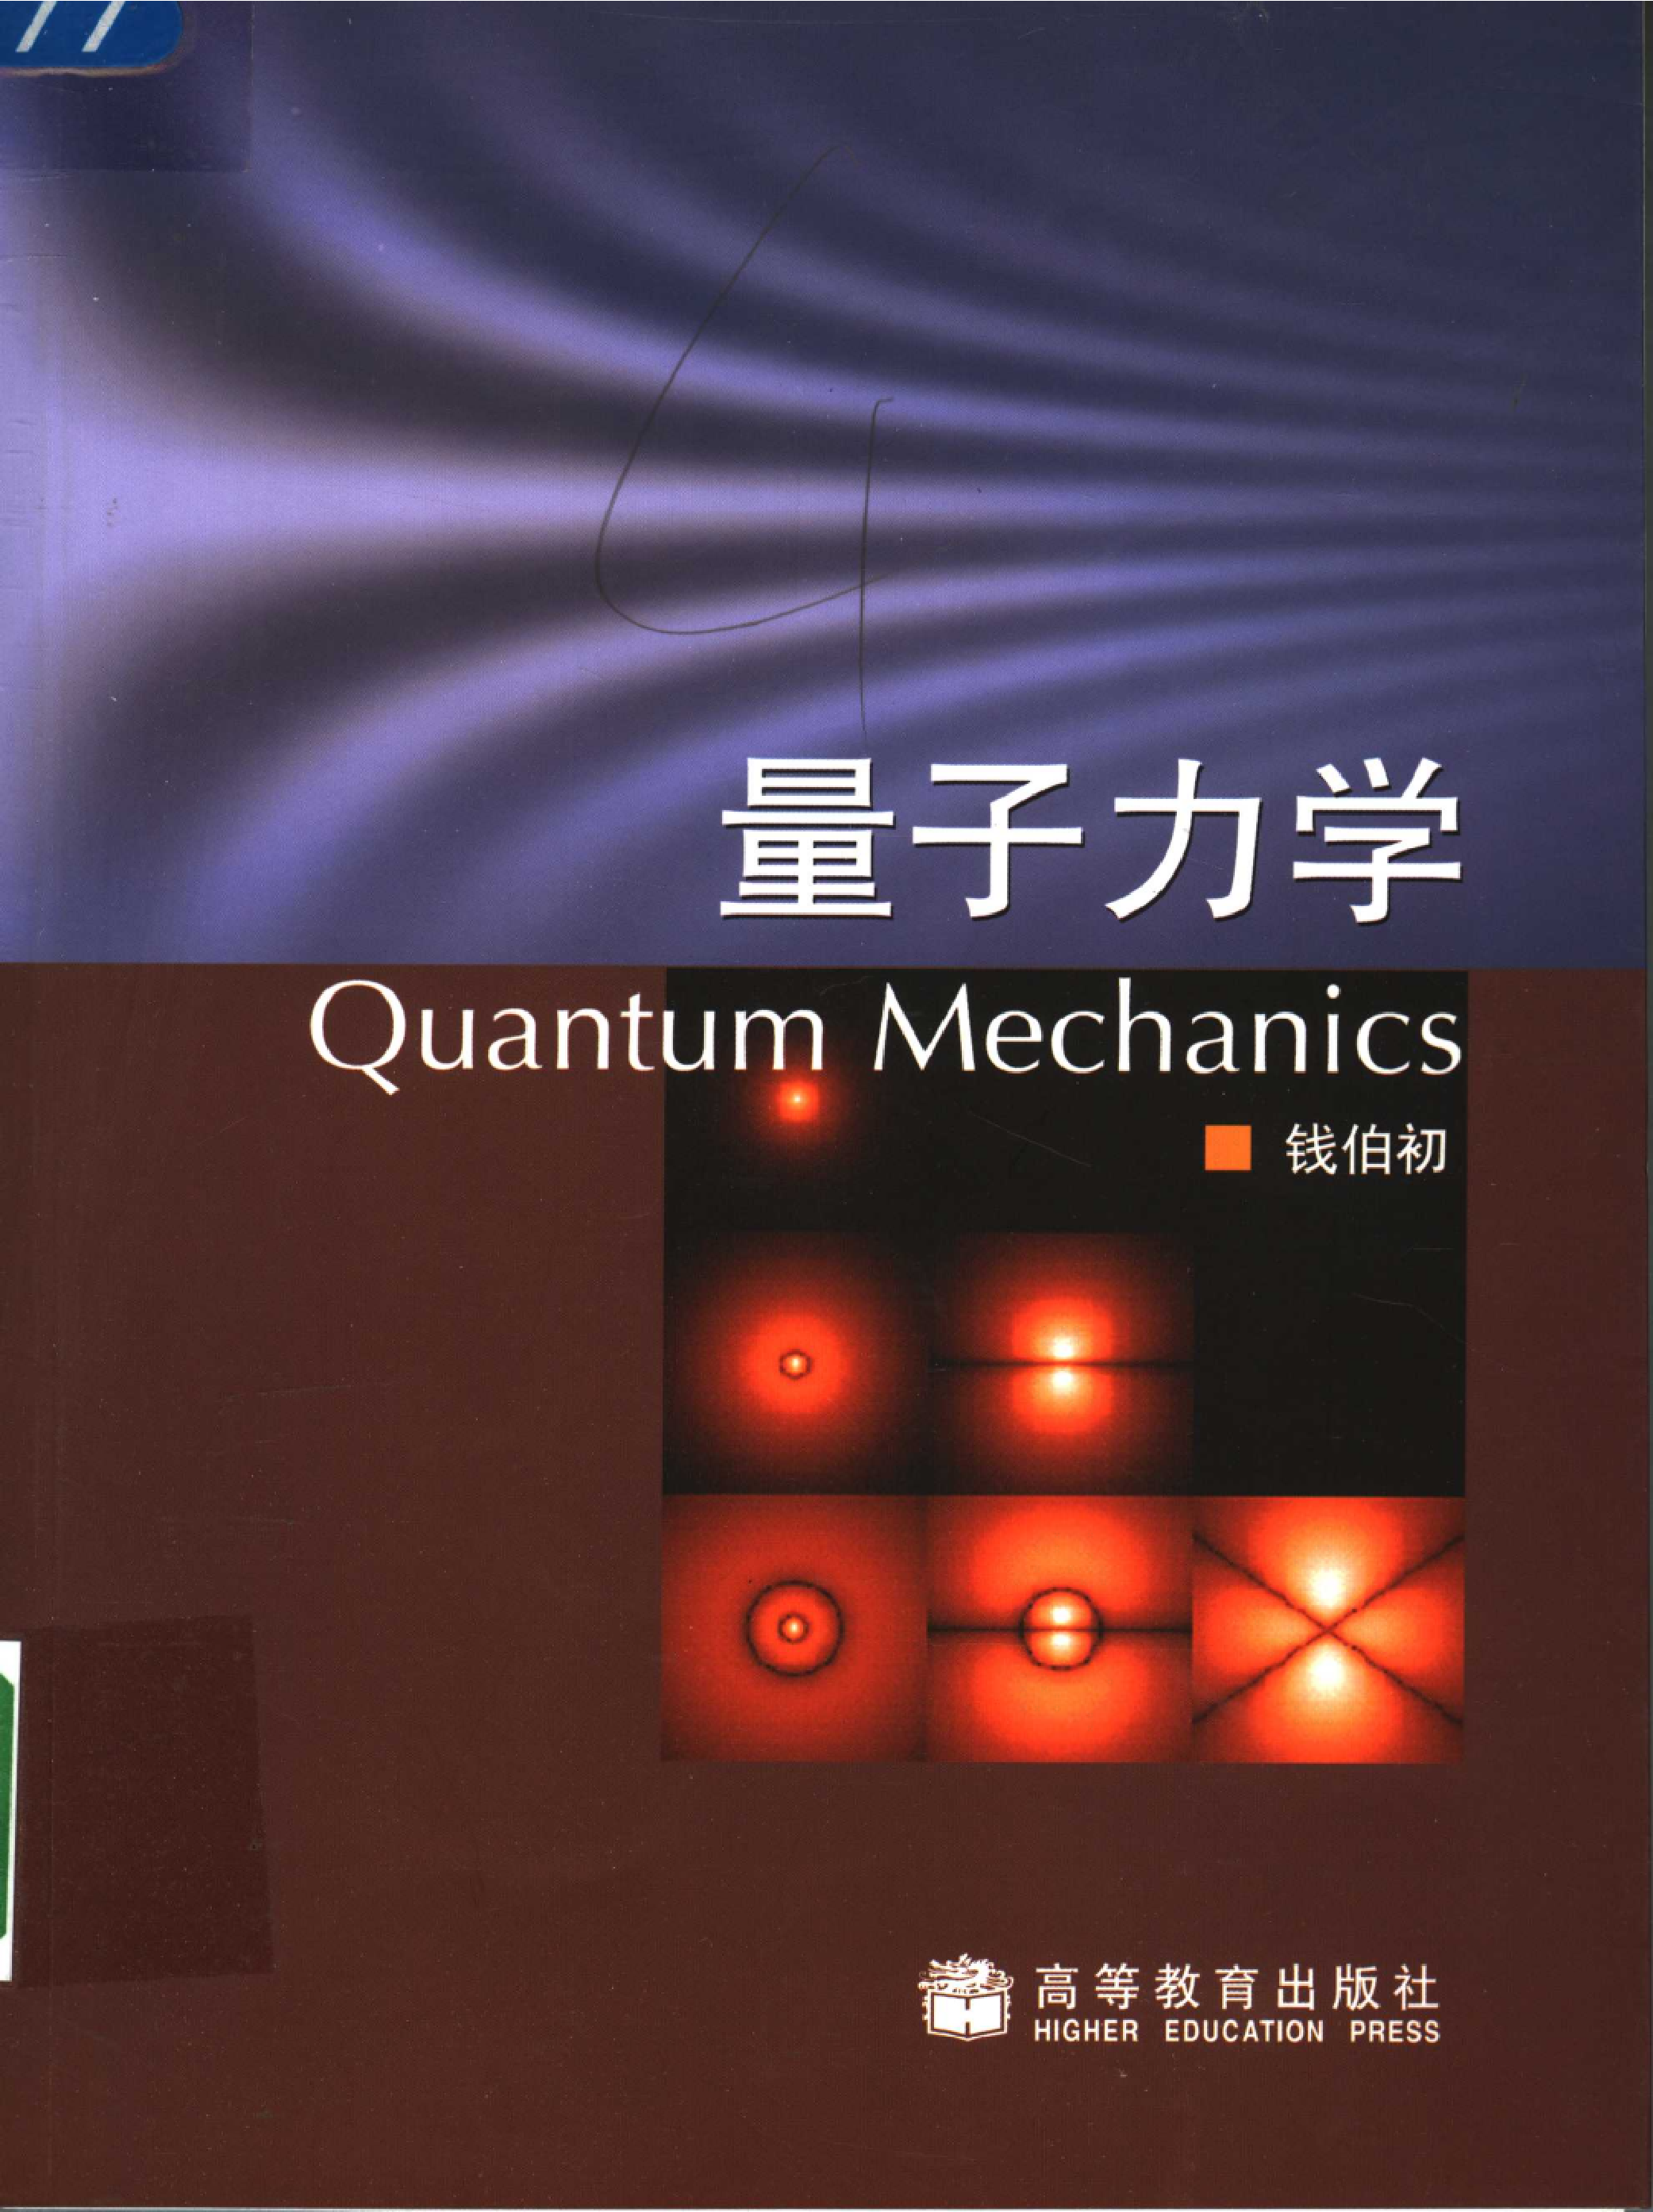
\includepdf{QM file/body/F00-Frontpage.pdf}
\bookmark[page=1,level=0]{封面}
%\clearpage\thispagestyle{empty}\cleardoublepage % 留白页

% 标题页
%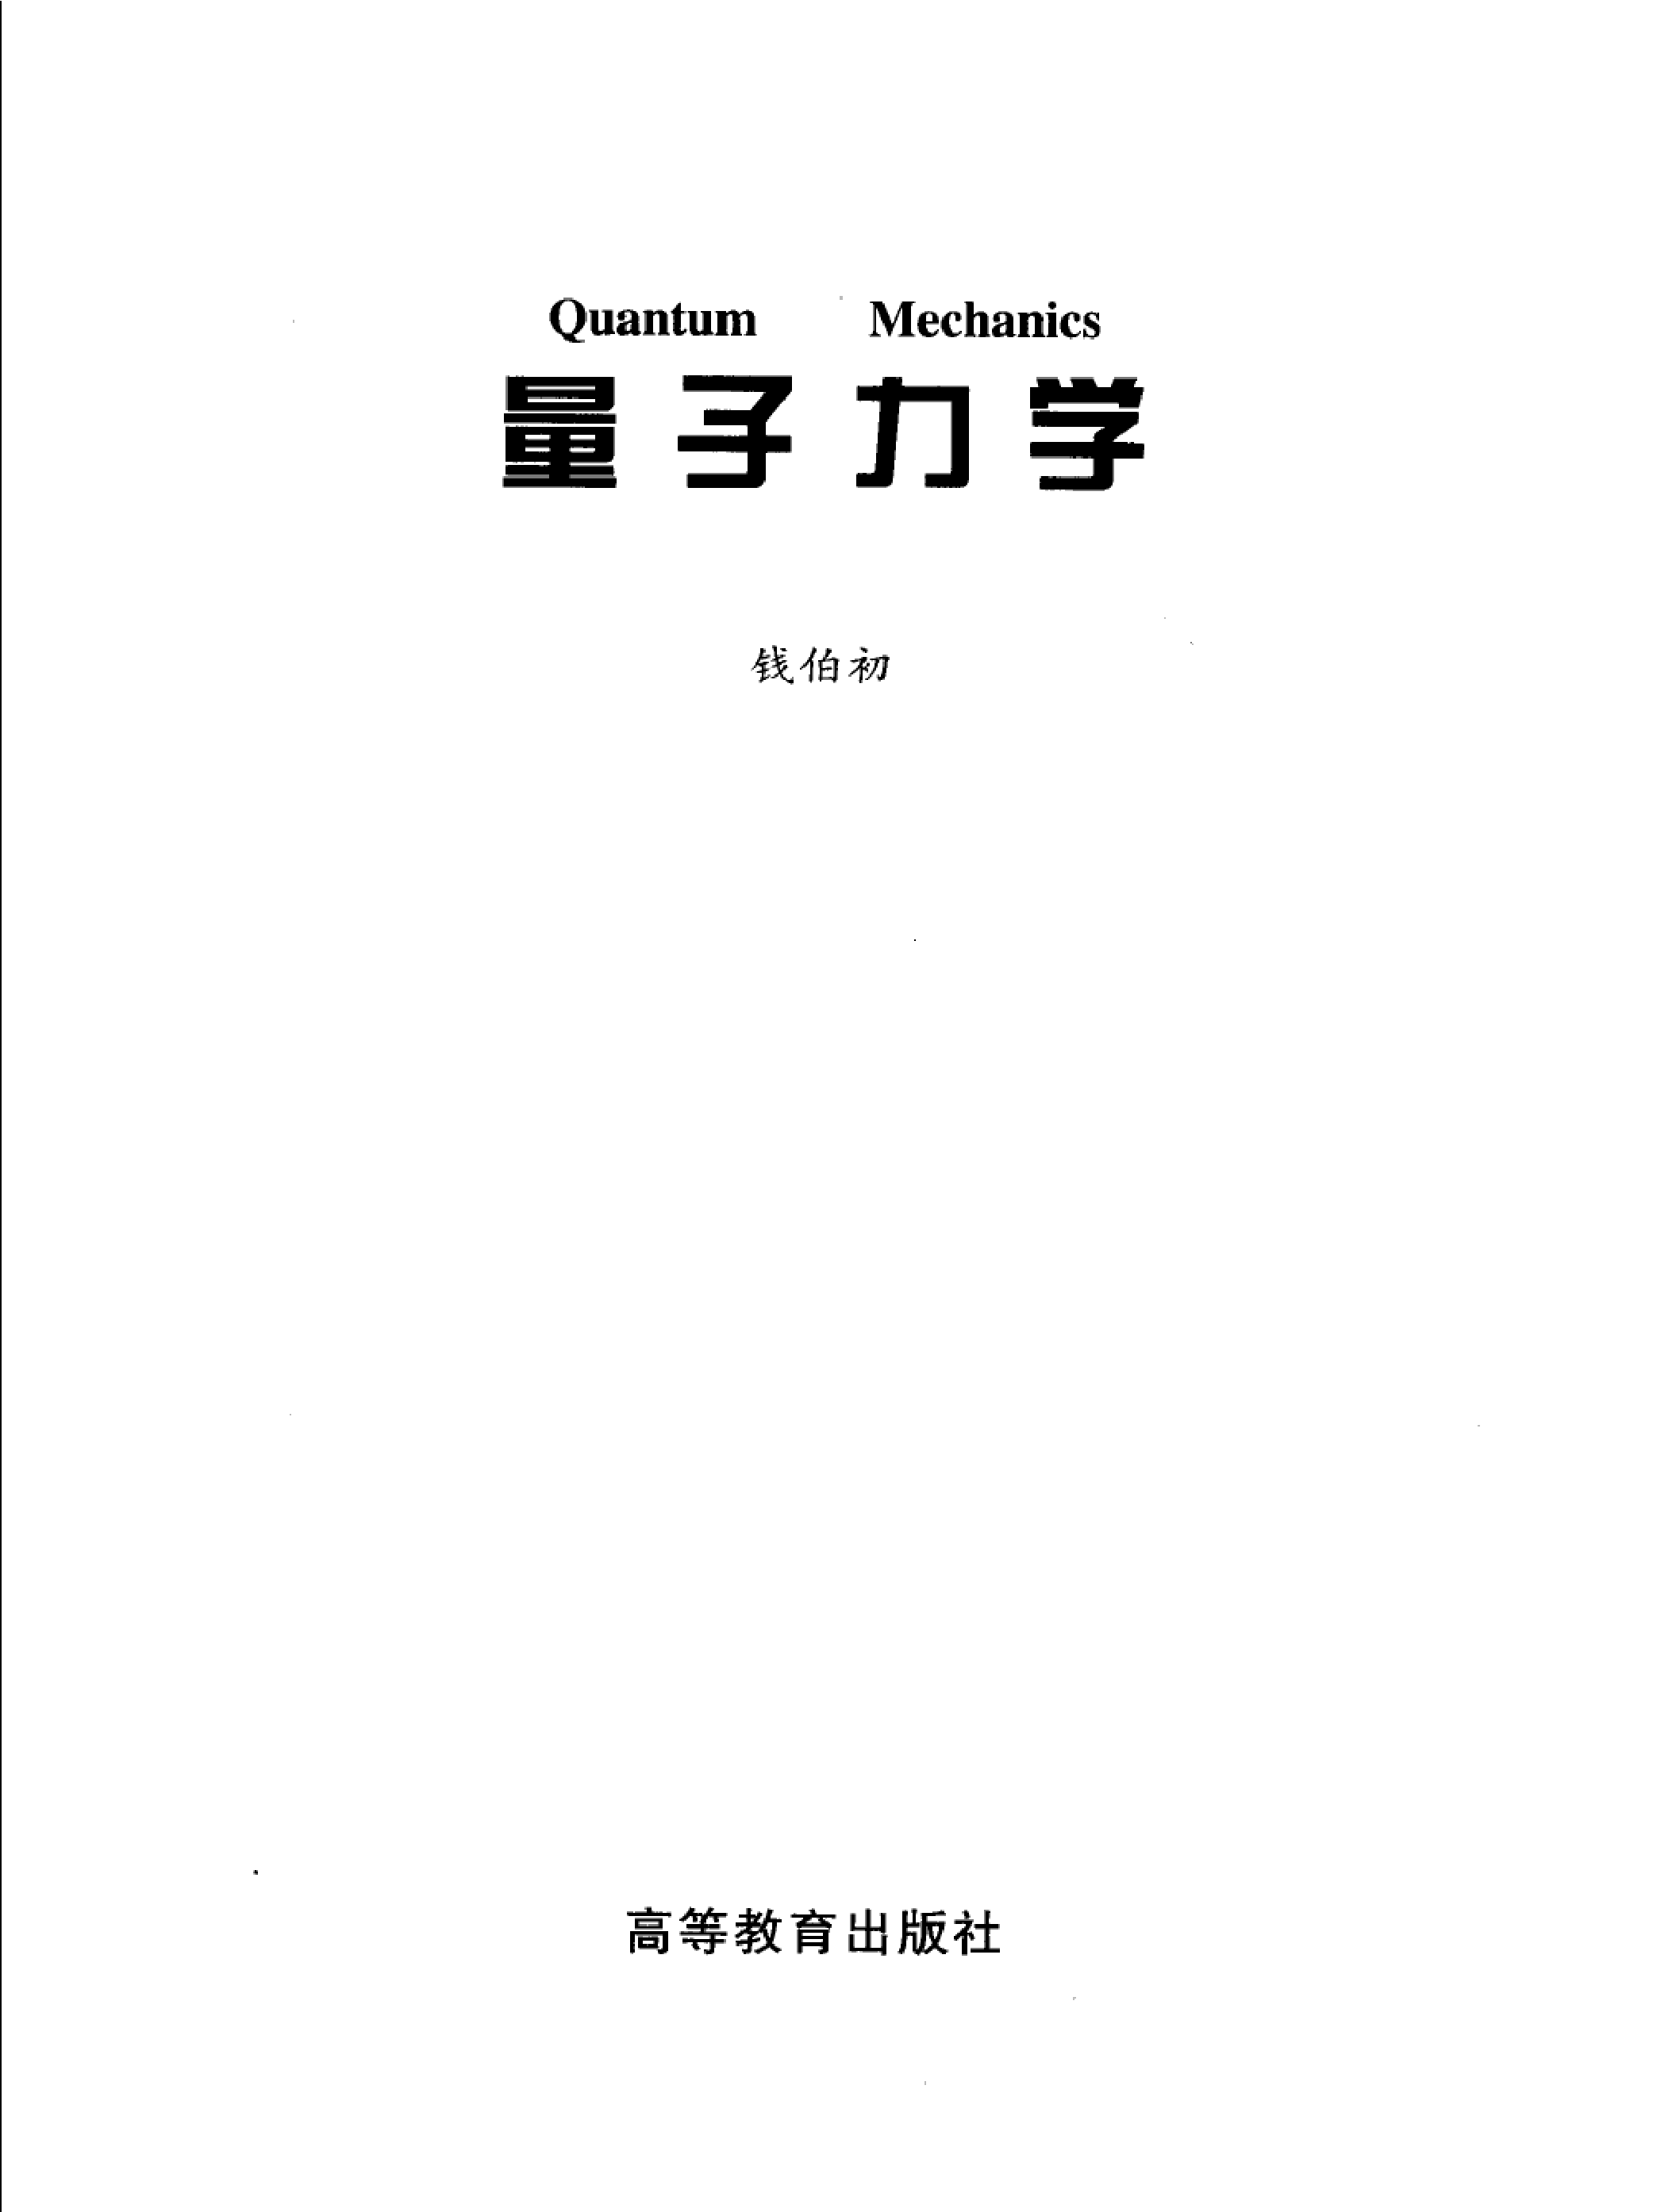
\includepdf{QM file/body/F01-Titlepage.pdf}
% 标题页
\begin{center}
		
	  \pskip
	
	\Large{Quantum \quad Mechanics} \par
	\Huge{\heiti 量~~子~~力~~学} \pskip
	
	\normalfont{}
	\normalsize
	
	
	\large \kaishu{钱伯初}
	
	\vfill
	%\zihao{5}
	\large{高~~~~等~~~~教~~~~育~~~~出~~~~版~~~~社}
	
\end{center}
\normalsize
\thispagestyle{empty}
\clearpage
\bookmark[page=2,level=0]{封页}

% 出版信息页
%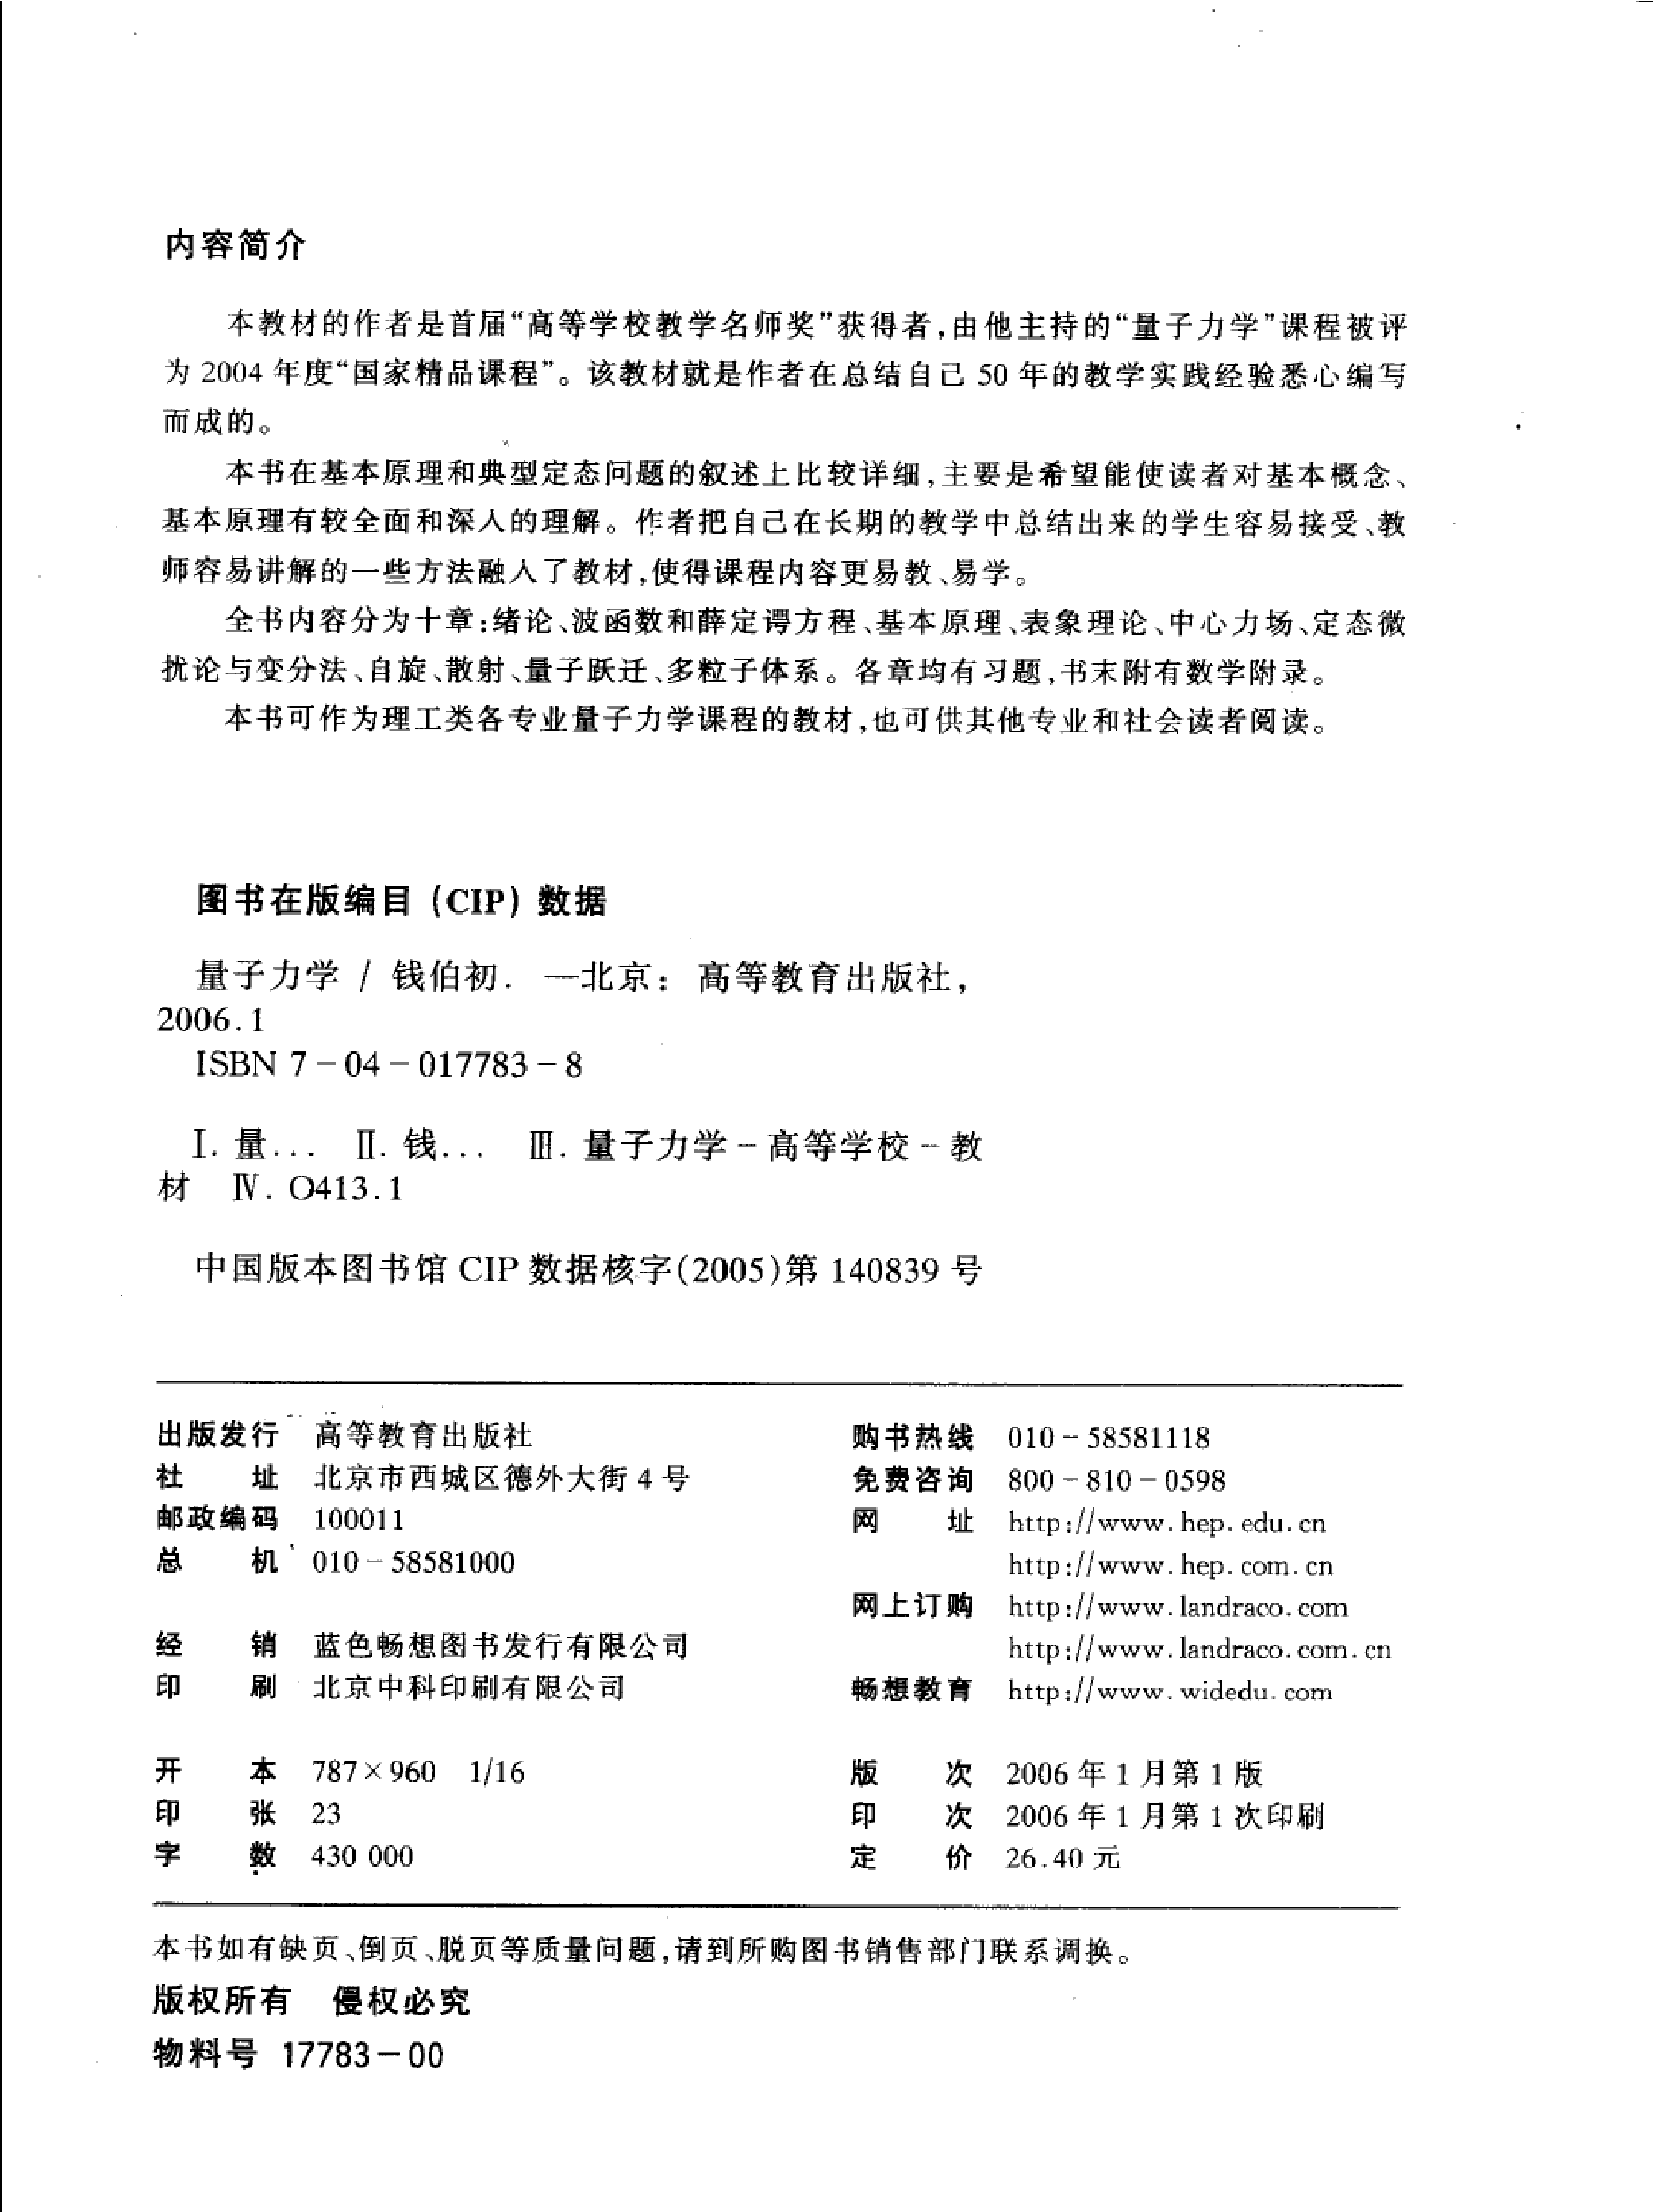
\includepdf{QM file/body/F02-Publish Information.pdf}
\input{QM file/body/F02-Publish Information}


% 前言
\input{QM file/body/F03-Foreword} 

% 目录
\clearpage
\setcounter{page}{1}
\pdfbookmark{目录}{Contents}
\tableofcontents

% 正文
\clearpage
\pagestyle{heading}
\setcounter{page}{1}
\setcounter{chapter}{-1}

% 公式与上下文本距离调整
\baselineskip=1.5em
\lineskip=0.25em
\lineskiplimit=0.25em
\abovedisplayskip=0.25em plus 0.25em minus 0.25em % 公式同上文间距
\belowdisplayskip=\abovedisplayskip				  % 公式同下文间距
\abovedisplayshortskip=0em plus 0.25em minus 0.25em
\belowdisplayshortskip=\abovedisplayshortskip
\belowcaptionskip=-0.8em % 原为-0.8em
\def\int{\mathop{\vcenter{\hbox{\scaleto[1.3ex]{\symbol{"222B}}{2em}}}}\nolimits}
\def\sum{\mathop{\vcenter{\hbox{\scaleto{\symbol{"2211}}{1.2em}}}}}


% 第一章 绪论
\setcounter{chapter}{0}
\chapter{绪论}\label{chp:01}
% \makebox[5em][s]{} % 短题目拉间距

量子力学是20世纪物理学最重要的发展,它和相对论一起,构成近代物理学的主要理论基础.

本章将扼要叙述量子力学诞生前早期量子论的要点,为系统叙述量子力学原理做些概念上的准备.有关史实及实验详情大都已在“原子物理学”课程中讲过,我们尽量从简,而将叙述的重点放在某些理论概念上.
% 黑体辐射与普朗克常数
\section[黑体辐射与普朗克常数]{黑体辐射与普朗克常数}\label{sec:01.01}
% \makebox[5em][s]{} % 短题目拉大字符
% \setlength{\mathindent}{9em} 本文标准公式缩进

在各种温度下,任何物体都能辐射出电磁波,同时也能吸收外界辐射来的电磁波.所谓黑体是指吸收本领最大的物体,它能全部吸收辐射到它表面上的电磁波.用热力学理论可以证明,黑体的热辐射本领也大于其他物体.空腔表面的小孔就是一种理想的黑体模型.

1789年,黑体热辐射的实验测量确定了著名的斯特藩(J.Stefan)四次方定律,1884年,玻尔兹曼从热力学理论上导出这条定律,因此,称此定律为斯特藩-玻尔兹曼定律:
\eqindent{12}
\begin{equation}\label{eq11.01}
	\boxed{J_{u}=\sigma T^{4}}
\end{equation}\eqnormal
$J_{u}$为热辐射能流通量(单位时间内单位表面积辐射出的电磁波能量),也称辐出度.$T$为黑体的热力学温度,$\sigma$为普适常量叫做斯特藩-玻尔兹曼常量,它与构成黑体的材料性质无关,其值为

\begin{wrapfigure}[4]{r}{9em}
	\centering
	\small
	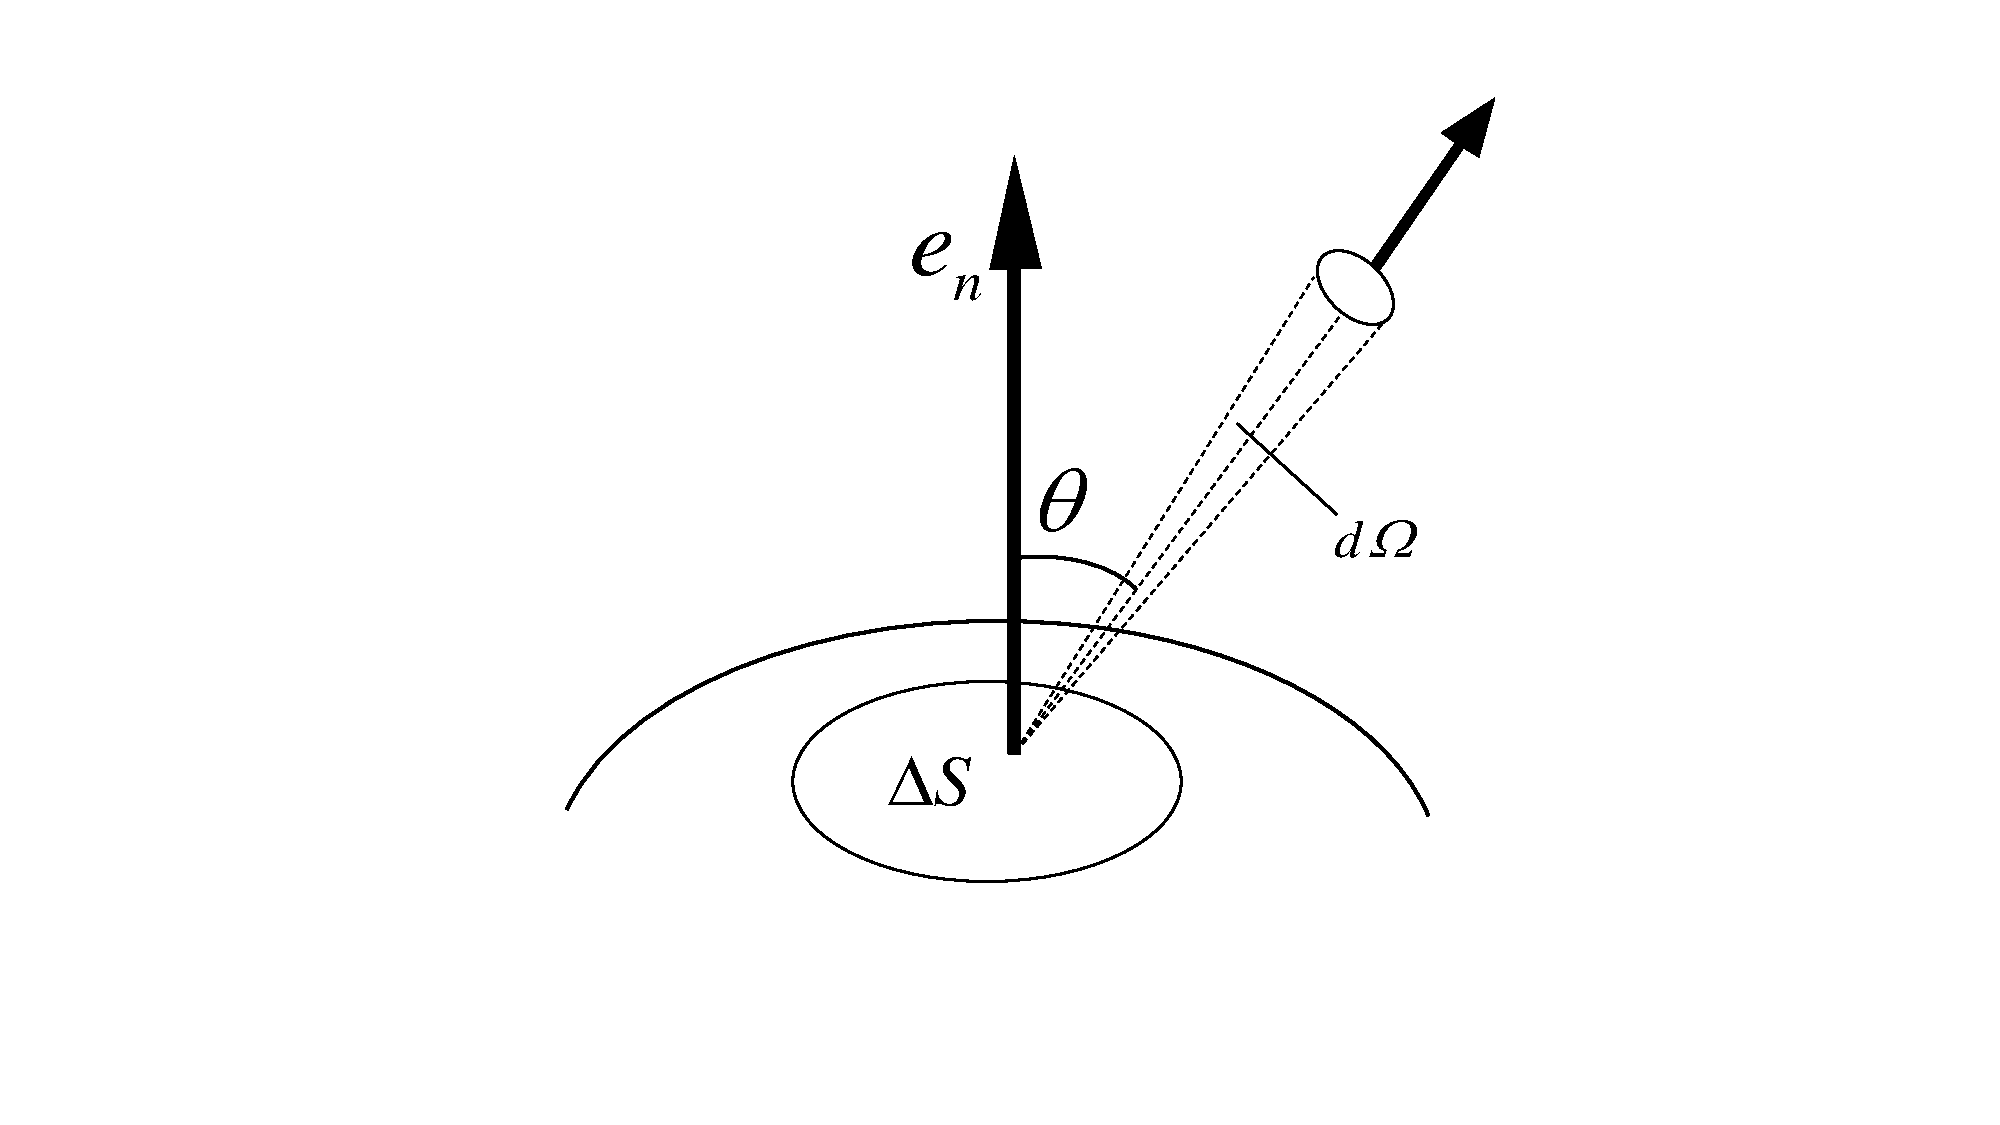
\includegraphics[width=2.5cm]{QM file/figure/1-1}
	\caption{}\label{fig.1-1}
\end{wrapfigure}
\eqindent{4}
\begin{equation*}
	\sigma=5.6704 \times 10^{-8} \si{W\cdot m^{-2} \cdot K^{-4}} 
\end{equation*}\eqnormal

图\ref{fig.1-1}是黑体辐射示意图,将空腔加热至温度$T$,这时腔内电磁场具有稳定的能量分布(各种频率的电磁波),经由小孔 $\Delta S$辐射出的能流可用仪器测出.如以$u$表示腔内电磁场能量密度(单位体积内电磁波能量),$c$表示光速,则单位时间内由$\Delta S$沿$d \Omega$方向辐射出的能量为
\begin{equation*}
	\Delta S\cdot \cos\theta\cdot cu\frac{d\Omega}{4\pi}
\end{equation*}
经$\Delta S$辐射出的总能量为
\begin{equation*}
	\begin{aligned}
		J_{u}\Delta S &=\int_{\theta \leq\frac{\pi}{2}}\Delta S \cos\theta cu \frac{d\Omega}{4\pi} \\
		&=\Delta S cu\frac{1}{4\pi}\int_{0}^{2\pi}d\varphi \int_{0}^{\frac{\pi}{2}}\cos\theta\sin\theta d\theta \\
		&= \frac{1}{4}cu\Delta S \\
	\end{aligned}
\end{equation*}
因此
\eqshort
\begin{equation}\label{eq11.02}
	u=\frac{4}{c}J_{u}=\frac{4\sigma}{c}T^{4}
\end{equation}
热辐射电磁场的能量密度与温度4次方成正比.注意比例系数为普适常数.

实验还可以测量出热辐射能量的频率分布.电磁波的波长$\lambda$与频率$\nu$及角频率$\omega=2\pi\nu$间有如下关系:
\begin{equation}\label{eq11.03}
	c=\lambda\nu=\frac{\lambda \omega}{2\pi}
\end{equation}
如以$\rho(\omega)d\omega$表示单位体积内角频率在$(\omega,\omega+d\omega)$间的电磁波能量,则能量密度$u$按$\omega$分布可以表示成
\begin{equation}\label{eq11.04}
	u=\int_{0}^{u} \rho(\omega)d\omega
\end{equation}\eqnormal
\begin{wrapfigure}[9]{r}{9em}
	\centering
	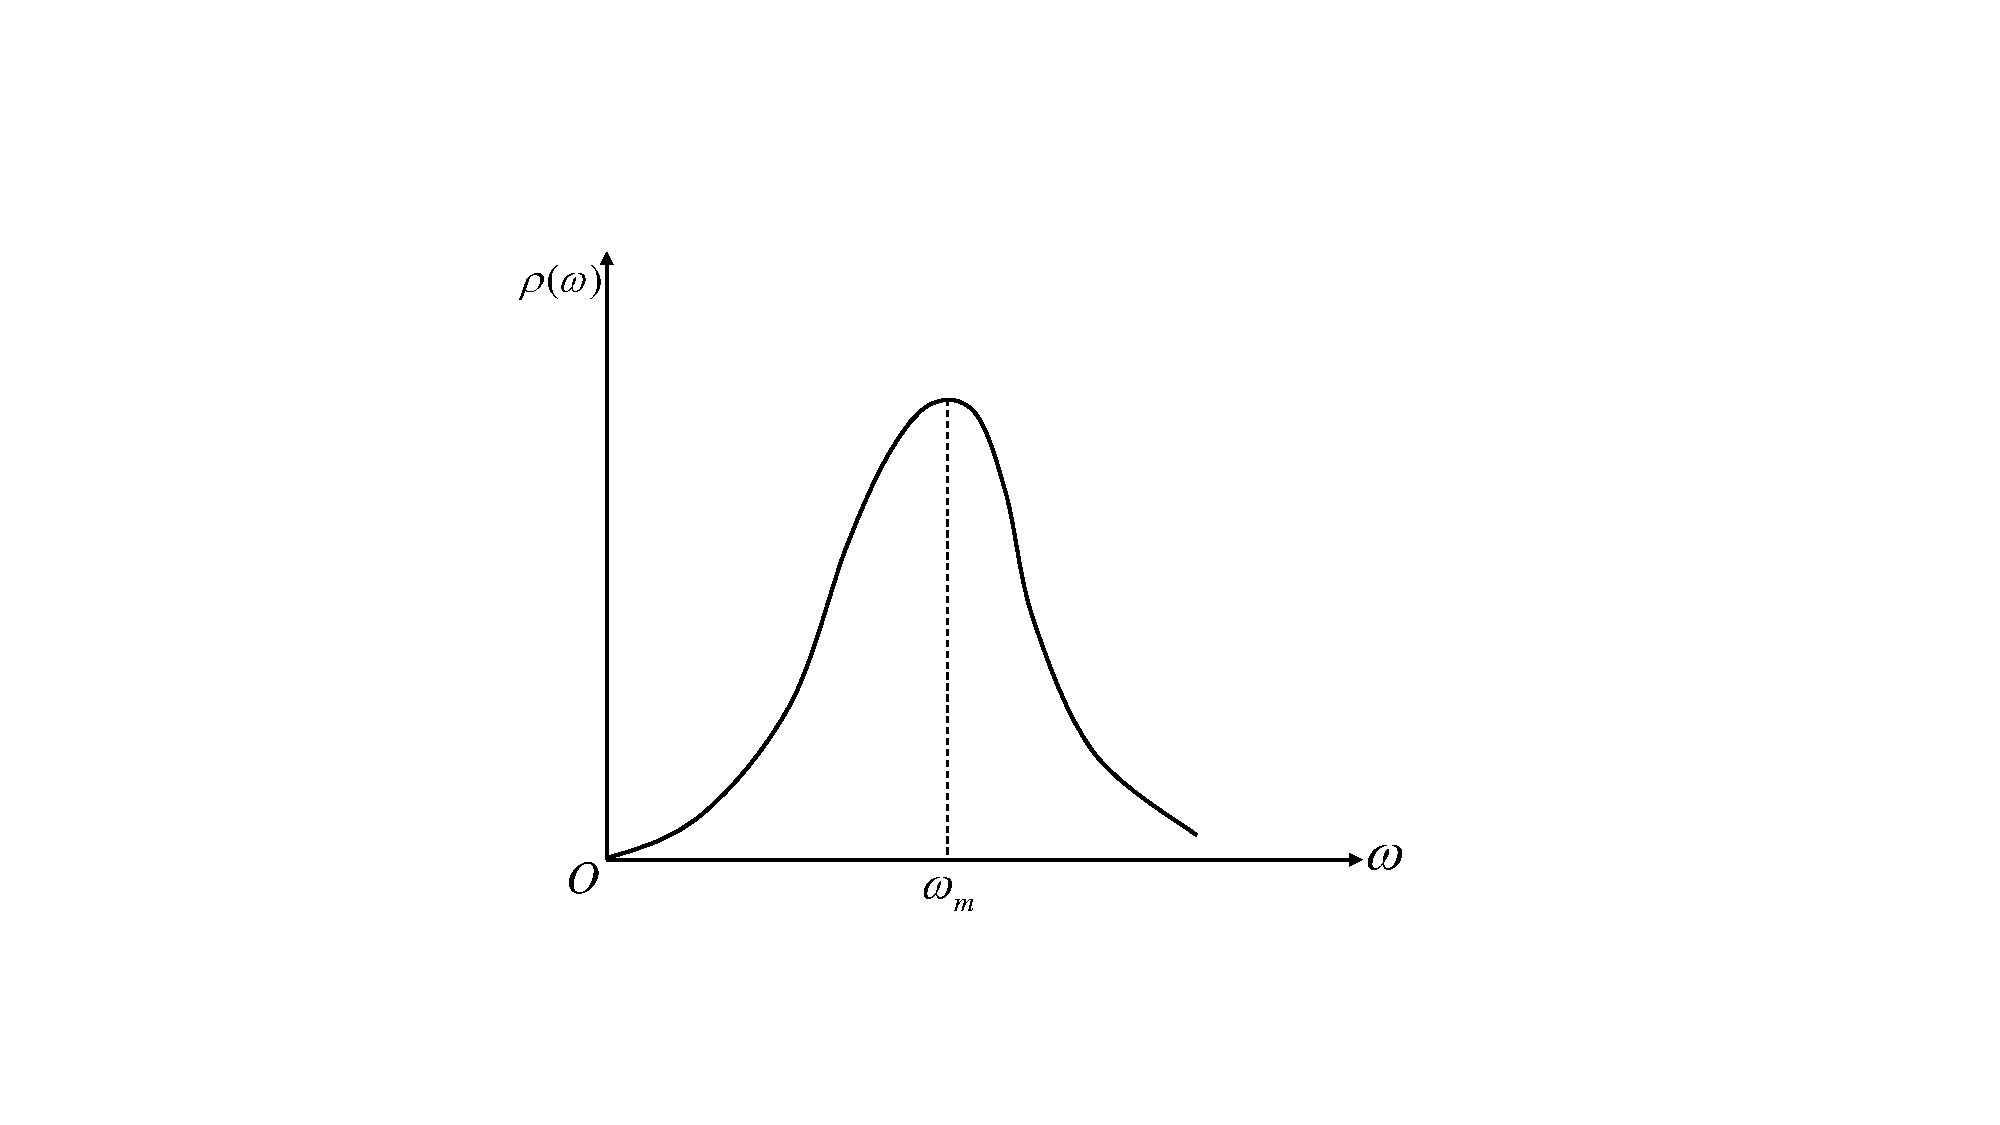
\includegraphics[width=3.5cm]{QM file/figure/1-2}
	\caption{}\label{fig.1-2}
\end{wrapfigure}

实验测得各种温度下$u$的频率分布曲线如图\ref{fig.1-2}所示.在长波部分$(\omega \rightarrow 0)\rho(\omega)\propto \omega^{2}T$;在短波部分$(\omega\rightarrow\infty)\rho(\omega)$随$\omega$之增大而迅速减小.对于每一种温度,$\rho(\omega)$都存在一个极大值,相应的角频率$\omega_{m}$和温度$T$成正比,相应的波长$(\lambda_{m}=\frac{2\pi c}{\omega_{m}})$和温度$T$成反比,
\eqindent{5}
\begin{equation}\label{eq11.05}
	T\lambda_{m}=5.1\times 10^{-3}  \si{m\cdot K}
\end{equation}\eqnormal
这规律称为维恩(W.Wein)位移定律.注意\eqref{eq11.05}式中的实验常数也是普适常量.

黑体辐射定律的发现引起了物理学界的极大关注,吸引力许多著名学者对它进行深入的理论探讨.当时经典物理学(牛顿力学,电磁学,热力学和经典统计物理是其主要内容)已经日臻成熟,权威物理学家大多相信经典物理学能够解释各类物理现象,黑体辐射定律应该也不例外.然而,冷酷的事实确是,企图在经典物理的理论框架内解释黑体辐射定律的努力,都在不同程度上遭到失败,其中最有成效的是瑞利和金斯(Rayleigh-Jeans)的研究.金斯利用波动理论,准确求得单位体积内$(\omega,\omega+d\omega)$范围内电磁振动模式总数,它等于
\eqindent{12}
\begin{equation}\label{eq11.06}
	\frac{\omega^{2}d\omega}{\pi^{2}c^{3}}
\end{equation}
\eqnormal
每一种电磁振动模式相当于一个简谐振子,在温度$T$下应该具有某种能量.按照经典统计物理的“能量均分定理”,温度$T$下简谐振子应该具有平均能量$kT$(k是玻尔兹曼常数).瑞利将“能量均分定理”用于热平衡下的电磁场(即热辐射场),从而得出结论:单位体积内$\omega,\omega+d\omega$范围内电磁振动能量应该是
\begin{equation}\label{eq11.07}
	\rho(\omega)d\omega=\frac{kT\omega^{2}d\omega}{\pi^{2}c^{3}}
\end{equation} 
这称为瑞利-金斯公式.这个公式在长波部分和实验曲线符合得极好,而在短波部分则和实验结果完全不符合.更严重的是,\eqref{eq11.07}式对$\omega$积分,将导致$u\rightarrow\infty$,这个结论显然是错误的.这就是历史上有名的“紫外发散困难”.

经历了许多失败,终于使物理学界认识到,为了解释黑体辐射定律,光靠经典物理学是不行的,必须有一个新的理论.这就是1900年普朗克(M.Planck)提出的量子论.

普朗克量子论的核心是下述“量子假设”:频率为$\nu$的电磁振动和原子、分子等物质发生能量转换时,能量不能连续变化,只能“量子”式地变化,每份“能量子”为
\begin{equation}\label{eq11.08}
	\varepsilon=h\nu=\hbar\omega \quad(\hbar=\frac{h}{2\pi})
\end{equation}
其中$h$是普适常数(后人称之为普朗克常数).在这假设下,普朗克利用热力学和统计物理理论,导出了著名地普朗克公式
\begin{equation}\label{eq11.09}
	\boxed{\rho(\omega)=\frac{\hbar\omega^{3}}{\pi^{2}c^{3}} \bigg/ (e^{\hbar\omega/kT}-1)}
\end{equation}

这个公式在各种温度下,全部频率范围内,均与实验曲线精确符合.历史上,普朗克导出\eqref{eq11.09}式的过程相当复杂.$\S$\ref{sec:09.04}将给出爱因斯坦对此式的简单证明.

普朗克的“量子假设”是和经典物理的整套概念抵触的.按照经典物理学,一切物质的运动变化都是连续进行的,能量变化也是连续的,这正是导致热平衡下“能量均分定理”的前提条件.普朗克舍弃了“能量均分定理”,代之以“量子假设”这在概念上是一次革命性的突破.从\eqref{eq11.09}式的结果看,由于能量的量子化,角频率为$\omega$的每一种电磁振动模式在温度$T$下的平均能量不再取“能量均分定理”给出的$kT$,而是
\begin{equation*}
	 E_{\omega}=\frac{\hbar\omega}{e^{\hbar\omega/kT}-1} 
\end{equation*}
在长波部分,$\hbar\omega\ll kT$,上式给出$\bar{E}_{\omega}\simeq kT$,与能量均分定理的结论一致.在短波部分,$\hbar\omega\gg kT$,上式给出
\begin{equation*}
	 \bar{E}_{\omega}\simeq \hbar\omega e^{\hbar\omega/kT} \ll kT 
\end{equation*}
这意味着高频振动被“冻结”,很难获得能量,因此避免了“紫外发散困难”.当一种电磁振动模式(角频率$\omega$)具有能量$E_{\omega}$时,相应的“能量子”数目为$n_{\omega}=\frac{E_{\omega}}{\hbar\omega}$,\eqref{eq11.09}式相当于“能量子”数的平均值为
\eqshort
\begin{equation}\label{eq11.10}
	\bar{n}_{\omega}=\frac{1}{e^{\hbar\omega/kT}-1}
\end{equation}
当$\hbar\omega\ll kT$,$\bar{n}_{\omega}=\simeq\frac{kT}{\hbar\omega}\gg 1$,电磁振动的能量变化近似于连续变化,量子论的结果和经典物理结果一致,当$\hbar\omega\gtrsim kT$,$\bar{n}_{\omega}<1$,量子论的结果和经典物理结果有本质差别.

\eqref{eq11.09}式代入\eqref{eq11.04}式,可以算出热辐射电磁场能量密度:
\begin{equation}\label{eq11.11}
	u=\frac{\pi^{2}(kT)^{4}}{15(\hbar c)^{3}}
\end{equation}\eqnormal
这结果与斯特藩-玻尔兹曼定律一致.

普朗克的“量子假设”是与整个经典物理格格不入的,使许多习惯于经典物理思维模式的资深物理学家感到难以接受.普朗克本人就曾花了多年时间研究能否不要“量子假设”,而在经典物理的范围内导出\eqref{eq11.09}式,结论是不能.显然,这意味着黑体辐射现象的后面隐藏着一种新的物理规律,这就是今天所谓的量子力学规律.

在这里,我们将用量纲分析方法证明黑体辐射定律绝不可能在经典物理学的框架范围内得到解释.

物理学的发展历史表明,每一种基本物理规律,均伴有相应的普适常数.例如代表万有引力定律的普适常数是引力常数$G$,代表电磁规律和相对论的基本普适常数是光速$c$,代表统计物理规律的基本普适常数是玻尔兹曼常数$k$,等等.如果黑体辐射定律可由经典物理来解释,有关的理论将是电磁学和统计物理,则在辐射场能量密度$u$的构造式中,只能包含$c,k,T$ $L,t,E,K$分别表示长度,时间,能量,温度的量纲,有关各量的量纲如下:
\begin{gather*}
	u——  \si{EL^{-3}},\qquad \qquad c——  \si{Lt^{-1}}  \\
	k——  \si{EK^{-1}},\qquad \qquad kT—— \si{E}  \\
	\sigma——  \si{Et^{-1}L^{-2}K^{-4}}
\end{gather*}
从量纲关系看,$u$显然不能由$c,k,T$构成,$\sigma$(普适常数)不可能由$c,k$构成.根据\eqref{eq11.02}式,可以判断$u\propto(kT)^{4}$,而从$u,c$与长度的量纲关系来看,可以设想$u\propto c^{-3}$,因此,$u\propto(kT)^{4}c^{-3}$.而$uc^{3}(kT)^{-4}$的量纲为$\si{(Et)^{-3}}$.如果设想黑体辐射现象涉及一种新的(未知的)基本物理规律,相应的基本普适常量(记为$\hbar$)量纲为$\si{Et}$,则$u$的构造式可以设想为
\eqshort
\begin{equation}\label{eq11.12}
	u=A(kT)^{4}(\hbar c)^{-3}
\end{equation}
其中$A$为无量纲纯数,结合\eqref{eq11.02}式,可得斯特藩-玻尔兹曼常数的构造式为
\begin{equation}\label{eq11.13}
	\sigma=\frac{A}{4}k^{4}\hbar^{-3}c^{-2}
\end{equation}\eqnormal
读者当然已经想到,这里提到的代表新规律的基本普适常数$\hbar$正好就是普朗克常数.事实上,如略去\eqref{eq11.12}、\eqref{eq11.13}式中不太重要的纯数$A$,利用$c,k,\sigma$的实验值,由\eqref{eq11.13}式即可估算出$\hbar \sim1.2\times 10^{-34} \si{J\cdot s}$,这正是普朗克常数$\frac{h}{2\pi}$的量级.如按精确计算得到的\eqref{eq11.11}式,[相当于\eqref{eq11.12}、\eqref{eq11.13}式中取$A=\frac{\pi^{2}}{15}$]则如上所述可以算出
\setlength{\mathindent}{4em}
\begin{equation*}
	\hbar=1.0546\times 10^{-34} \si{J\cdot s},\quad h=2\pi\hbar=6.6262\times 10^{-34} \si{J\cdot s}
\end{equation*}
\setlength{\mathindent}{9em}
这数值与普朗克常数的精密测量值非常接近.

\example 试用普朗克公式\eqref{eq11.09}求$\rho(\omega)$极大值对应的角频率$\omega_{m}$与温度$T$的数值关系,并估算热辐射场的光子数密度.

\solution $\rho(\omega)$取极大值时,满足极值条件$\frac{\partial \rho}{\partial \omega}=0$.令$x=\frac{\hbar\omega}{kT}$,极值条件亦即
\eqshort
\begin{equation*}
	\frac{d}{dx}\frac{x^{3}}{e^{x}-1}=0
\end{equation*}
由此得出$x$满足的方程为
\begin{equation*}
	\frac{x}{3}=1-e^{-x}
\end{equation*}
用数值解法可解出$x=\num{2.8214}$,因此
\begin{equation}\label{eq11.14}
	\frac{\hbar\omega_{m}}{kT}=\num{2.8214}
\end{equation}\eqnormal
这正是维恩位移定律.读者不难验证\eqref{eq11.14}式与\eqref{eq11.05}式是一致的.

由于辐射场的能量集中分布在$\omega\sim\omega_{m}$附近,所以光子数密度(单位体积内光子数)可估计成
\begin{equation}\label{eq11.15}
	n\sim\frac{u}{\hbar\omega_{m}}\sim\frac{\pi^{2}}{15\times2.82}\bigl(\frac{kT}{\hbar c}\bigr)^{3}\sim 0.23\bigl(\frac{kT}{\hbar c}\bigr)^{3}
\end{equation}
精确结果是
\begin{equation}\label{eq11.16}
	n=\int_{0}^{\infty}\frac{\rho(\omega)}{\hbar\omega}d\omega=0.2436\bigl(\frac{kT}{\hbar c}\bigr)^{3}
\end{equation}

从量纲关系看,$n$的构造式中只能包含$kT,c,\hbar$,他们的量纲是
\begin{equation*}
	n——\si{L^{-3}},\quad kT—— \si{E},\quad \hbar c—— \si{EL} 
\end{equation*}
所以唯一可能的量纲构造关系是$n\sim\bigl( \frac{kT}{\hbar c} \bigr)^{3}$









% 光子
\section[光子]{\makebox[5em][s]{光子}}\label{sec:01.02}
% \makebox[5em][s]{} % 短题目拉间距
% \setlength{\mathindent}{9em} 本文标准公式缩进

1905年,爱因斯坦将普朗克的量子假设发展成光量子(光子)的概念也正是这一年,爱因斯坦创立了狭义相对论.

爱因斯坦认为,电磁波(光波)的结构应该是量子化的,其最小单元即一个光子,每个光子均以同样的速度$c$(光速)运动频率为$v$的光波,其光子的能量和动量为
\begin{align}
	E=h\nu=\hbar\omega \label{eqn:01.02.01} \\ 
	p\approx \frac{E}{c}=\frac{h\nu}{c}=\frac{h}{\lambda} \label{eqn:01.02.02}
\end{align}
$\lambda$为光波的波长,光子的运动方向应该和光波的传播方向一致.

对于单色平面波,如引入“波矢量”$\boldsymbol{k}$,其方向为波的传播方向,其数值为$k=| \boldsymbol{k}|=\frac{2\pi}{\lambda}$,则光子的动量可以表示成
\eqindent{12}
\begin{equation}\label{eqn:01.02.03}
	\boldsymbol{p}=\hbar \boldsymbol{k}
\end{equation}\eqnormal

光和其他物质发生相互作用时,基元过程通常表现为光子-电子作用或者光子-原子作用,利用光子的概念并对作用过程应用能量守恒定律,一般就能够得出某些(但不是全部)重要结论.

\textsf{1. 光电效应}

某些金属受到光的照射后,能够发射出电子,形成电流,这就是光电效应其物理机理可用光子概念解释如下金属中的“自由电子”要逸出金属表面,需要克服“逸出功”,$W$当金属受到频率为$v$的光照射时,自由电子即可吸收光子,从而获得能量(电子同时或在短时间内连续吸收两个以上光子的机会极小,可以不考虑这种可能性.)如$h\nu>W$,电子就可以从金属中逸出,并具有动能
\begin{equation}\label{eqn:01.02.04}
	\boxed{\frac{1}{2}m_{c}v^{2}=h\nu-W}
\end{equation}
由此可见,光电子的动能完全由逸出功$W$(由金属性质决定)和入射光的频率$v$所决定,而与光的强度无关光电子的数目则与入射光的强度成正比,即和入射光子的总数成正比对光电子动能的实验测量完全证实了爱因斯坦公式\eqref{eqn:01.02.04}的正确性由\eqref{eqn:01.02.04}式还可看出,当逸出功$W$给定后,入射光的频率$v$必须超过$W/h$,才能产生光电效应;如$v<\frac{W}{h}$,尽管光很强,也不会产生光电子这个结论也已为实验证实.

\textsf{2. 康普顿散射}

关于光子能量和动量的爱因斯坦公式\eqref{eqn:01.02.01}、\eqref{eqn:01.02.03},于l923年被康普顿(A.H.Compton)散射所证实实验发现,X射线被石蜡等轻物质散射时,波长增大经典电磁理论很难解释这现象康普顿利用光子的概念,并假定在光子-电子作用过程中,能量守恒定律和动量守恒定律成立,利用相对论力学,对散射过程作出了成功的理论分析.

$X$射线的光子能量,约在$10^{3}\si{eV}$以上轻物质中外层电子的原子能级仅几个电子伏,可以当作自由电子设$X$射线的入射波长为$\lambda$,则入射光子的能量、动量为
\begin{equation} 
	\begin{aligned} \notag
		E=h\nu=\frac{hc}{\lambda} \\
		p=\frac{E}{c}=\frac{h\nu}{c}=\frac{h}{\lambda}
	\end{aligned}
\end{equation}
\begin{wrapfigure}[7]{r}{9em}
	\centering
	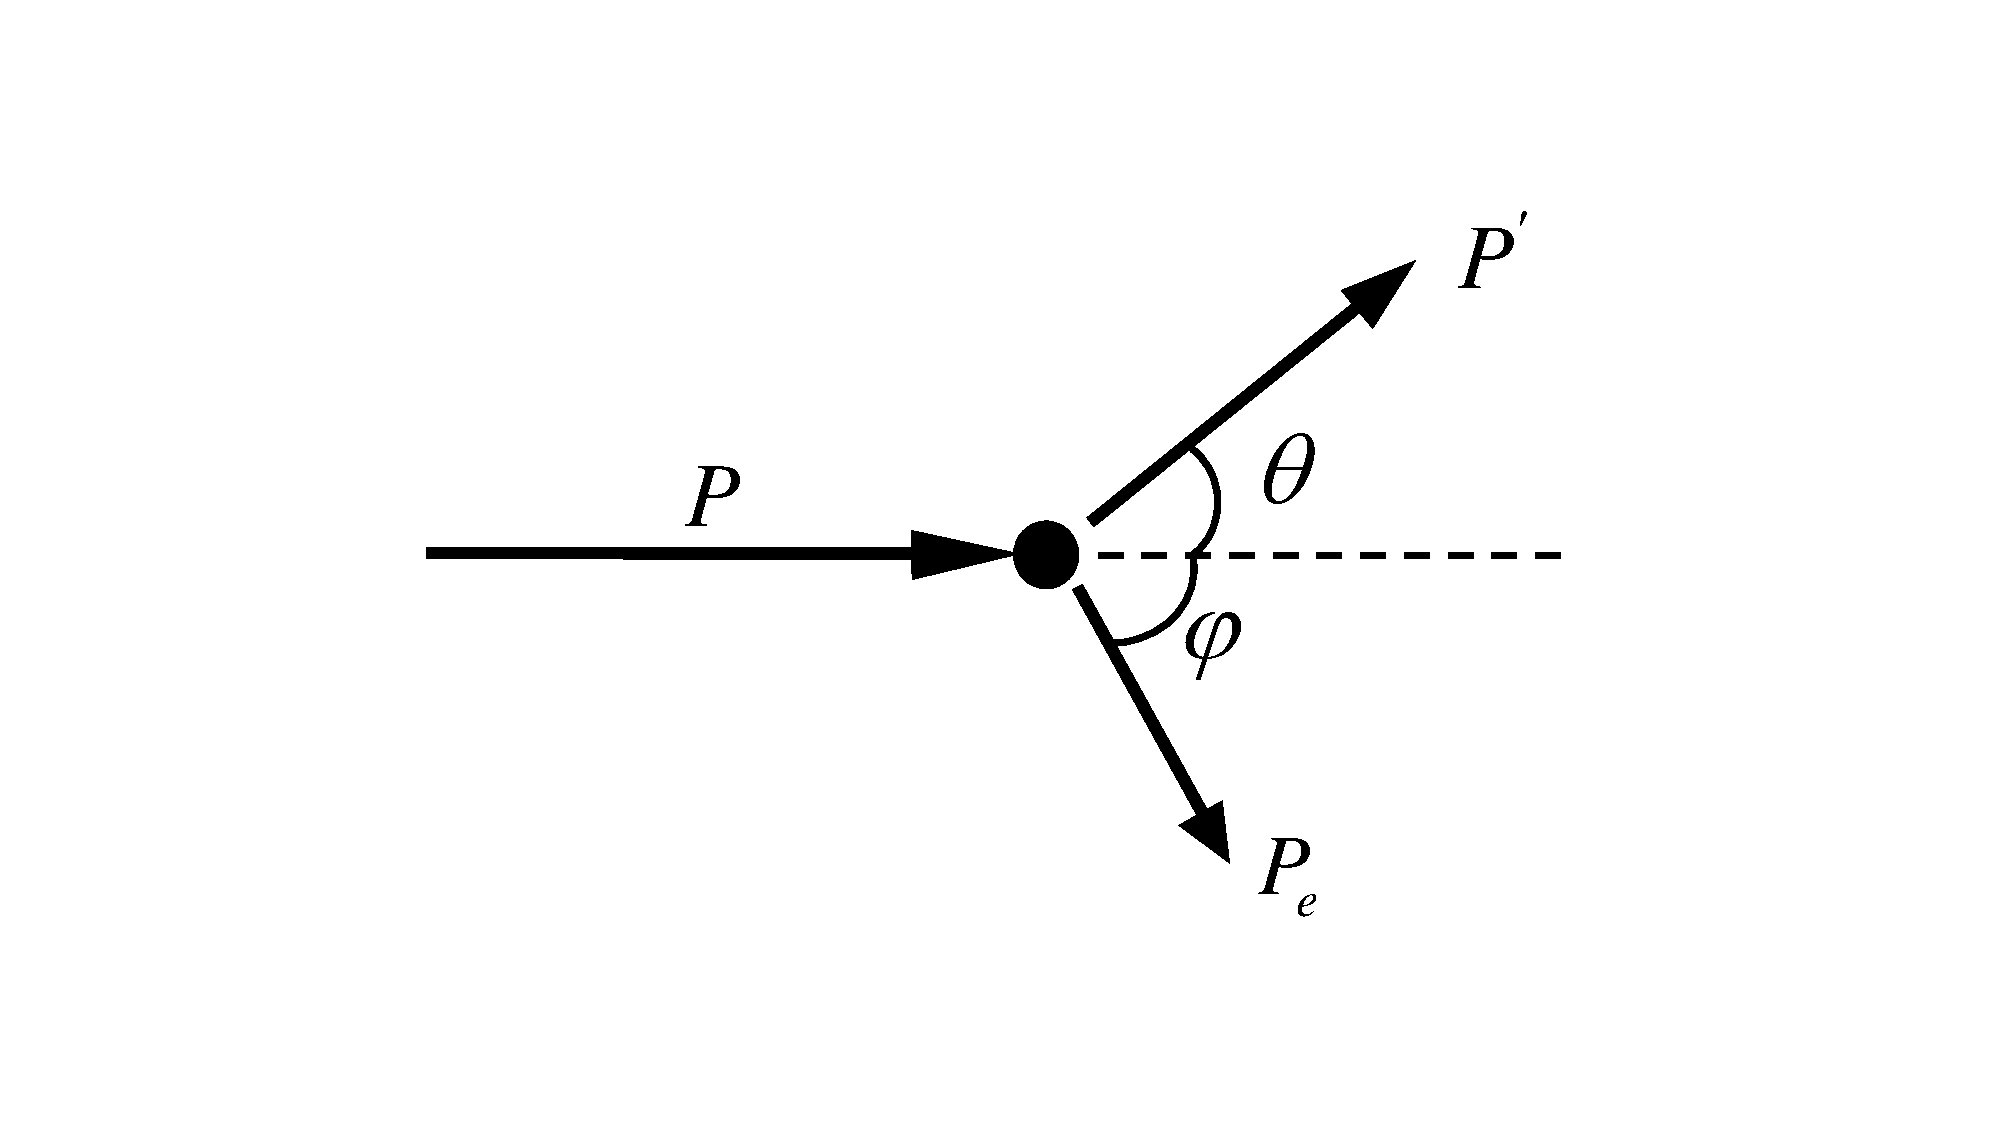
\includegraphics[width=3cm]{QM file/figure/1-3}
	\caption{}
	\label{fig.1-3}
\end{wrapfigure}
电子初始动量为0,初始能量为$m_{c}c^{2}$散射(碰撞)后,设光子沿$\theta$方向射出,如图\ref{fig.1-3},波长变为$\lambda^{\prime}$,能量及动量变为
\setlength{\mathindent}{6em}
\begin{equation}
	\begin{aligned} \notag
		E^{\prime}=h\nu^{\prime}=\frac{hc}{\lambda^{\prime}} \\
		p^{\prime}=\frac{E^{\prime}}{c}=\frac{h\nu^{\prime}}{c}=\frac{h}{\lambda^{\prime}}
	\end{aligned}
\end{equation}
\eqnormal
电子的反冲角设为$\varphi$能量和动量设为$E_{e}$和$p_{e}$,按照相对论力学
\begin{equation}\label{eqn:01.02.05}
	E_{e}^2=c^{2}p_{e}^{2}+m_{e}^{2}c^{4}
\end{equation}
对散射过程应用能量守恒定律,得到
\begin{equation*}
	h\nu+m_{e}c^{2}=h\nu^{\prime}+E_{e}^{2}
\end{equation*}
亦即
\begin{equation}\label{eqn:01.02.06}
	h(\nu-\nu^{\prime})=E_{e}-m_{e}c^{2}
\end{equation}
对散射过程应用动量守恒定律,得到
\begin{equation}\label{eqn:01.02.07}
	\boldmath p-p^{\prime}=p_{e}
\end{equation}
取平方,得到
\begin{equation*}
	p^{2}+p^{\prime 2}-2\boldsymbol{p}\cdot\boldsymbol{p^{\prime}}=p_{e}^{2}
\end{equation*}
亦即
\begin{equation}\label{eqn:01.02.08}
	h^{2}(\nu+\nu^{\prime}-2\nu\nu^{\prime}\cos\theta)=E_{e}^{2}-m_{e}^{2}c^{4}
\end{equation}
\eqref{eqn:01.02.06}式取平方,则得
\begin{equation*}
	h^{2}(\nu+\nu^{\prime}-2v\nu^{\prime})=(E_{e}-m_{e}c^{2})^{2}
\end{equation*}
与\eqref{eqn:01.02.08}式相消,得到
\begin{equation}
	\begin{aligned}
		2h^{2}\nu\nu^{\prime}(1-\cos\theta) &=2m_{e}c^{2}(E_{e}-m_{e}c^{2}) \\
		&=2m_{e}c^{2}h(\nu-\nu^{\prime})
	\end{aligned}
\end{equation}
因此,
\begin{equation*}
	\frac{1}{\nu}-\frac{1}{\nu^{\prime}}=\frac{h}{m_{e}c^{2}}(1-\cos\theta)
\end{equation*}
亦即
\begin{equation}\label{eqn:01.02.09}
	\boxed{\lambda^{\prime}-\lambda=\frac{h}{m_{e}c}(1-\cos\theta)}
\end{equation}
经过散射,X射线得波长有所增加,增量$(\lambda^{\prime}-\lambda)$与散射角有关,并与$\frac{h}{m_{e}c}$成比例,后者称为康普顿波长,记为$\lambda_{c}$,
\begin{equation}\label{eqn:01.02.10}
	\lambda_{c}=\frac{h}{m_{e}c}=2.43\times10^{-12} \si{m}
\end{equation}
对散射光波长的实验证实了\eqref{eqn:01.02.09}式的正确性因此,康普顿散射证实了:(i)光子的能量、动量公式\eqref{eqn:01.02.01}、\eqref{eqn:01.02.02}、\eqref{eqn:01.02.03}是正确的;(ii)微观基元过程中,能量守恒定律和动量守恒定律成立;(iii)相对论力学是正确的.

\textsf{3. 粒子-反粒子对的湮没与产生}

实验发现,电子($e^{-}$)及其反粒子(正电子,$e^{+}$)相碰,可以湮没而产生两个$\gamma$光子,即
\begin{equation*}
	e^{-}+e^{+}\rightarrow \gamma+\gamma
\end{equation*}
根据相对论力学及能量、动量守恒定律,每个$\gamma$光子的能量至少等于电子的静能,即$E_{r}\geqslant m_{e}c^{2}$,相应的$\gamma$射线波长为
\begin{equation*}
	\lambda=\frac{hc}{E_{r}}\leqslant\frac{h}{m_{e}c}=\lambda_{c}
\end{equation*}
这个关系已为实验所证实粒子物理的理论分析表明,能够产生上述湮没过程的电子、正电子距离,大致也是康普顿波长的量级.

在温度$T$下,热辐射光子的平均能量约为$3kT$(k为玻尔兹曼常数)按照近代天体物理理论,在宇宙形成的初期,温度极高,两个光子相碰,可能转变成(质子、反质子)对或(中子,反中子)对,按照能量守恒定律,有
\begin{equation*}
	E_{\gamma}\approx3kT\approx m_{p}c^{2}=938 \si{MeV}
\end{equation*}
因此当时温度约为
\begin{equation*}
	T\approx m_{p}c^{2} \big/ 3k\approx3.6\times10^{12} \si{K}
\end{equation*}




% 玻尔的量子论
\section[玻尔的量子论]{玻尔的量子论}\label{sec:01.03}
% \makebox[5em][s]{} % 短题目拉间距
% \setlength{\mathindent}{9em} 本文标准公式缩进 
% \eqnormal % 恢复标准缩进

\textsf{1. 氢原子光谱}

19世纪后期,广泛进行了原子光谱的实验研究.1885年,巴尔末(Balmer)在氢原子光谱中发现了一个谱线系,其频率可以精确地表示成
\begin{equation}\label{eqn:01.03.01}
	\nu=\frac{c}{\lambda}=cR\bigg( \frac{1}{2^2}-\frac{1}{n^2} \bigg),\quad n=3,4,5,\cdots
\end{equation}
其中
\begin{equation*}
	R=\num{10967758.1} \si{m^{-1}} \text{(里德伯常数)}
\end{equation*}
后来又发现了其他谱线系.总的说,氢原子光谱全部谱线的频率可以归结成公式
\setlength{\mathindent}{6em}
\begin{equation}\label{eqn:01.03.02}
	\nu=\frac{c}{\lambda}=cR\bigg( \frac{1}{m^2}-\frac{1}{n^2} \bigg),\quad m<n \text{($m,n$为正整数)}
\end{equation}
\eqnormal
光谱公式虽然是经验公式,但是其精确度极高,为任何其他定量公式所不及.因此有理由相信,在这些公式后面一定隐藏着某种深刻的物理规律.

\textsf{2. 卢瑟福原子模型}

\begin{wrapfigure}[7]{r}{6em}
	\centering
	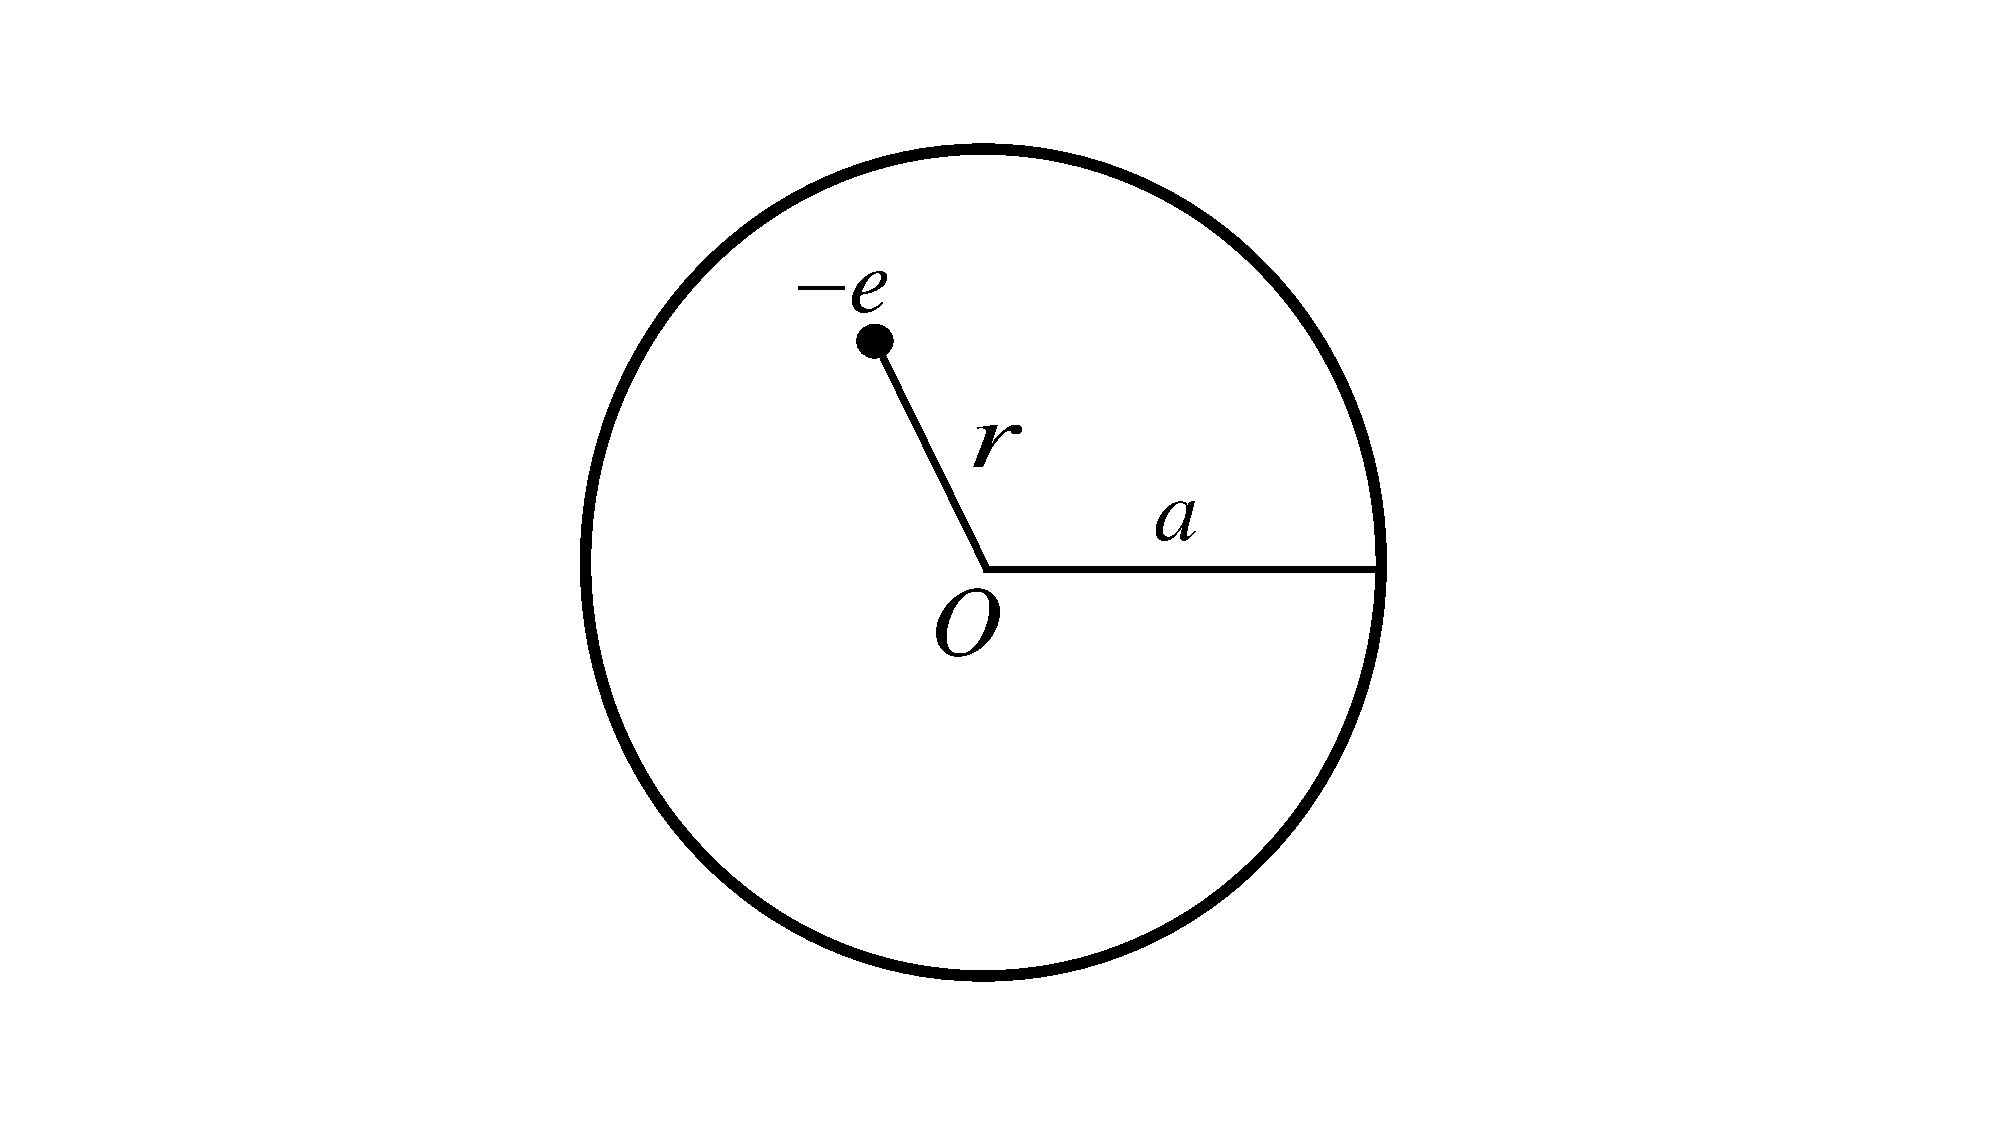
\includegraphics[width=2cm,clip]{QM file/figure/1-4}
	\caption{}
	\label{fig.1-4}
\end{wrapfigure}
1897年,汤姆孙(J.J.Tomson)用测量荷质比$\frac{e}{m_{e}}$的办法发现了电子.1903年,他顺理成章地提出了一种原子模型:原子的质量及正电荷均匀分布在球形体积中,球的半径即原子半径.电子(质量为$m_{e}$,远小于原子质量)在正电荷的库仑力作用下,可在原子内运动.按照汤姆孙原子模型,正常情况下电子停留在原子中心(球心),这时原子不发光.如因外力作用而使电子偏离了原子中心,正电荷对电子的库仑作用力将使电子在中心附近作简谐振动,从而向外辐射电磁波,即原子将发光.以单电子原子为例,如\ref{fig.1-4}所示,正电荷$Q=e$均匀分布在球内,电子(电荷$q=-e$)偏离球心时,库仑力为
\eqlong
\begin{equation}\label{eqn:01.03.03}
	\boldsymbol{F}=\-\frac{e^{2}}{4\pi\varepsilon_{0}}\bigg(\frac{r}{a} \bigg)^{3} \frac{r}{r^{3}}=-\frac{e^{2}}{4\pi\varepsilon_{0}}\frac{r}{a^{3}}
\end{equation}\eqnormal
今后,凡涉及库仑力问题,公式中$4\pi\varepsilon_{0}$一律省略不写.$\frac{e^{2}}{4\pi\varepsilon_{0}}$简记为$\e^{2}$.\eqref{eqn:01.03.03}式简写成
\eqshort
\begin{equation*}\label{eqn:01.03.03'}
	\boldsymbol{F}=-\frac{\e^{2}}{a^{3}} \boldsymbol{r} \tag{$1.3.3^{\prime}$}
\end{equation*}\eqnormal
库仑力表现为弹性力,因此电子将在球心附近作简谐运动,频率为
\eqlong
\begin{equation}\label{eqn:01.03.04}
	\nu=\frac{\omega}{2\pi}=\frac{1}{2\pi}\bigg(\frac{\e^2}{m_{e}a^3} \bigg)^{\frac{1}{2}}=\frac{1}{2\pi a}\bigg(\frac{\e^2}{m_{e}a^3} \bigg)^{\frac{1}{2}}
\end{equation}
电子振动时,将辐射出同样频率的电磁波,波长为
\begin{equation}\label{eqn:01.03.05}
	\lambda=\frac{c}{\nu}=2\pi ac\bigg(\frac{m_{e}a}{\e^2} \bigg)^{\frac{1}{2}}=2\pi a\bigg(\frac{a}{r_{e}} \bigg)^{\frac{1}{2}}
\end{equation}
其中为c光速,$r_{e}$为“经典电子半径”,
\begin{equation}\label{eqn:01.03.06}
	r_{e}=\frac{\e^2}{m_{e}c^{2}}=2.82\times10^{-15} \si{m}=2.82 \si{fm}
\end{equation}\eqnormal
如取原子半径$a\sim 0.1 \si{nm}=10^{-10} \si{m}$,求出
\begin{equation*}
	\lambda \sim 118 \si{nm},\quad \nu\sim 2.5\times10^{15} \si{s^{-1}}
\end{equation*}
属于紫外光区域.从数量级说,和原子光谱的范围大体相符.但是这种原子模型显然无法解释实验已经发现的氢原子光谱公式\eqref{eqn:01.03.02}.

汤姆孙原子模型终于被否定,是由于卢瑟福(Rutherford)的$\alpha$粒子对重元素的散射实验(1912)结果.

来自元素天然放射性的$\alpha$粒子,质量约为电子的7000倍,但比重元素的原子轻得多.因此在散射过程中,原子可以近似地当作是静止的.$\alpha$粒子的实验室动能约为几个$\si{MeV(10^{6} \si{eV})}$,远大于原子中电子的电离能(数量级$10\si{eV}$),因此当$\alpha$粒子与电子的距离接近到原子半径的量级时,即可使电子电离.只有原子中的正电荷才是使$\alpha$粒子发生散射的主要因素.

\begin{wrapfigure}[6]{r}{6em}
	\centering
	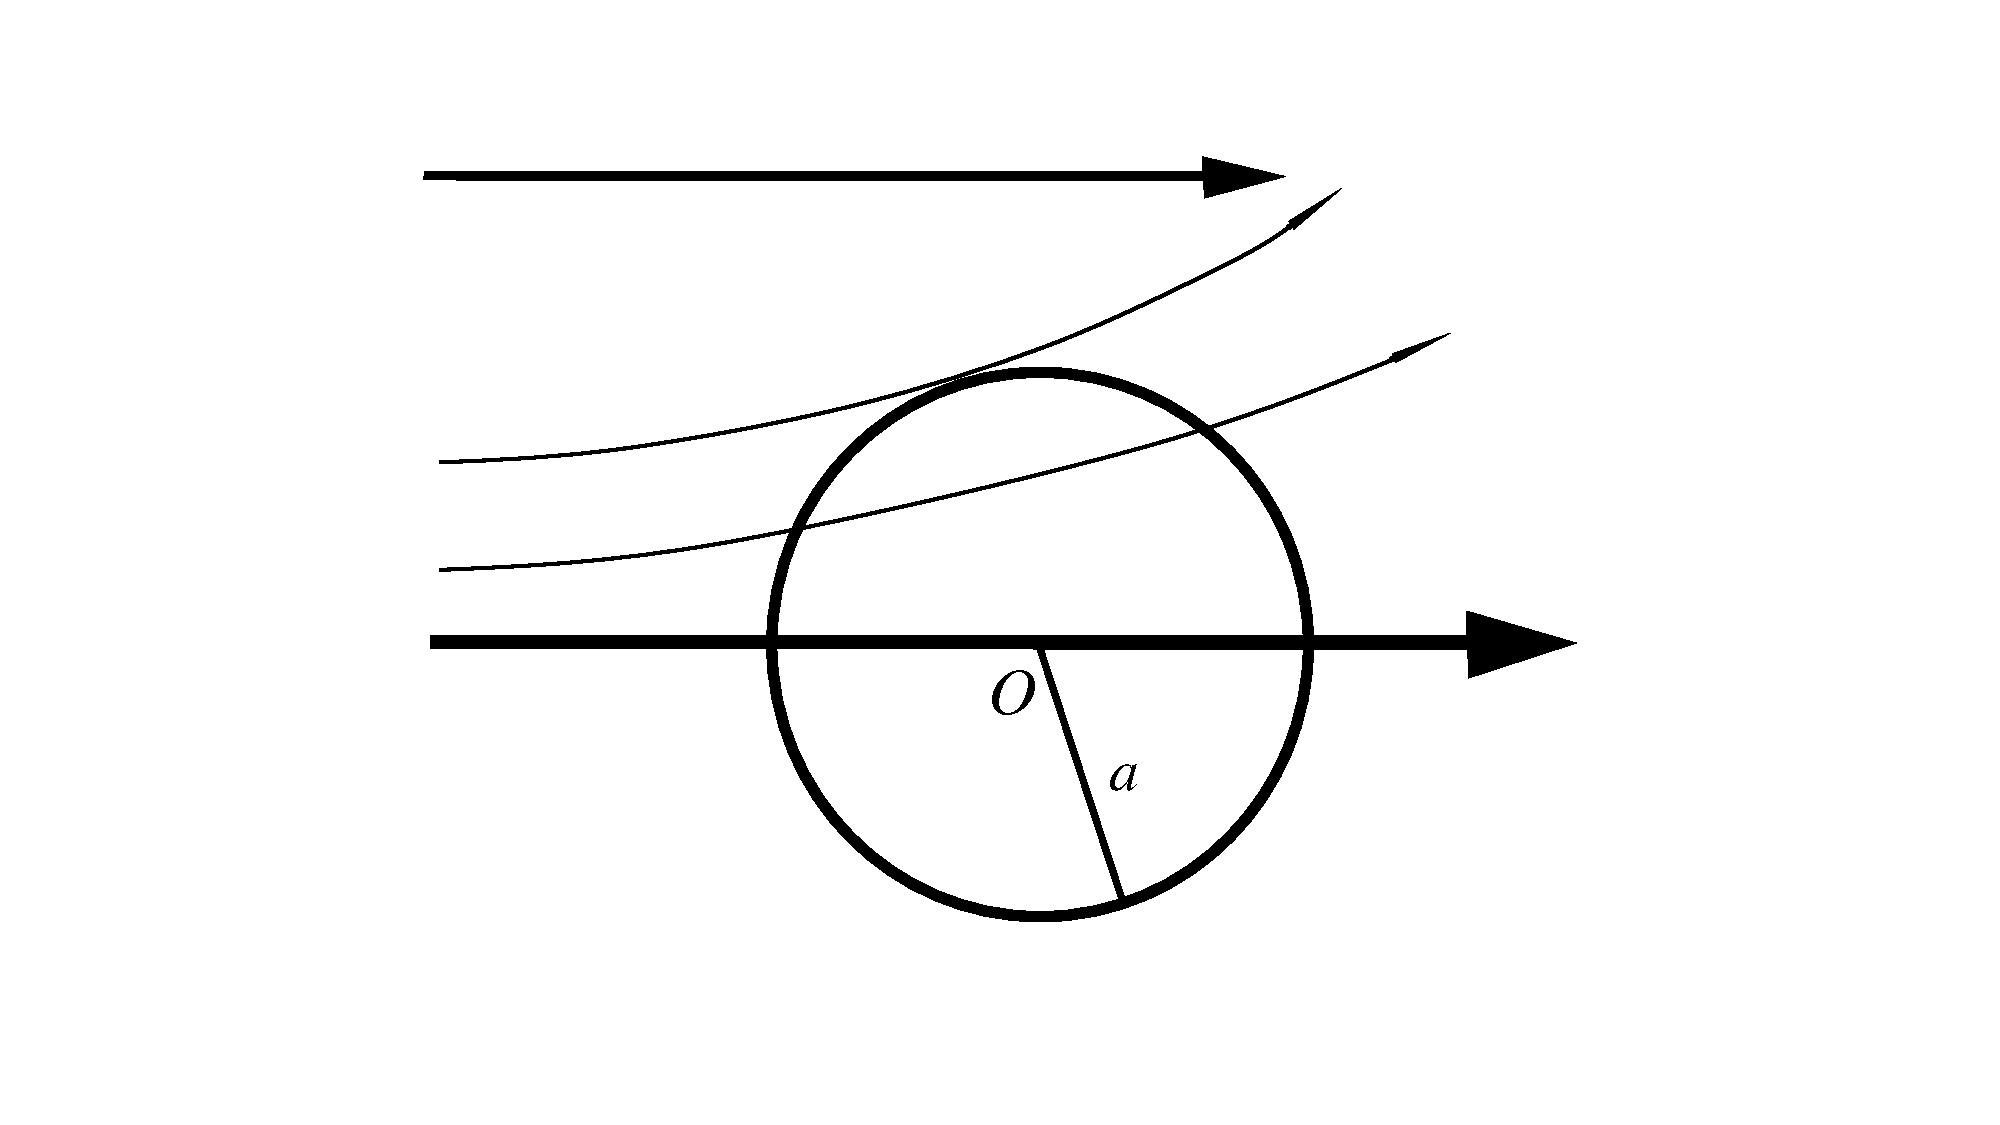
\includegraphics[width=2.5cm,clip]{QM file/figure/1-5}
	\caption{}
	\label{fig.1-5}
\end{wrapfigure}
令一束$\alpha$粒子以相同的初速度$v_{o}$射向一个汤姆孙原子,原子的正电荷($Q=Ze$,Z为原子序数)以库仑力作用于$\alpha$粒子,力的横向分量使$\alpha$粒子运动方向发生偏转.显然,在正电荷边缘掠过的$\alpha$粒子受到的横向力最大,偏转角也最大,如\ref{fig.1-5}所示.下面估算一下最大偏转角的量级.最大横向力约为
\begin{equation*}
	F_{\perp}\sim 2\e\cdot\frac{Z\e}{a^{2}}
\end{equation*}
有效作用时间约为$t\sim\frac{2a}{v_{0}}$,由此获得的横向动量约为
\begin{equation*}
	p_{\perp}\sim F_{\perp}\cdot t \sim\frac{4Z\e^{2}}{av_{0}}
\end{equation*}
因此,最大偏转角约为
\begin{equation}\label{eqn:01.03.07}
	\theta_{max}\sim \frac{p_{\perp}}{m_{a}v_{0}}\sim\frac{4Z\e^{2}}{m_{a}v_{0}^{2}a}=\frac{2Z\e^{2}/a}{E}
\end{equation}
其中$E=\frac{1}{2}m_{a}v_{0}^{2}$是$\alpha$粒子入射动能,$\frac{2Z\e^{2}}{a}$是最大静电势能.

以$\alpha$粒子被金原子(Z=79)散射为例,如取$a\sim 0.1\si{nm}$,$E\sim 5\si{MeV}$,则
\begin{gather}
	\frac{2Z\e^{2}}{a}\sim 2.3\times10^{-3} \si{MeV} \notag \\
	\theta_{max}\sim 4.6\times10^{-4} \notag
\end{gather}
而实验发现,最大偏转角可以超过$\frac{\pi}{2}$,甚至接近$\pi$.对实验结果的统计分析表明,这种大偏转角绝非多次散射的结果,而是由单次散射造成的.由此可知,原子中正电荷的分布半径应该远小于原子半径.为了解释大偏转角散射,原子中正电荷分布半径$R_{0}$应该满足关系:
\setlength{\mathindent}{12em}
\begin{equation}\label{eqn:01.03.08}
	\frac{2Z\e^{2}}{R_{0}} > E
\end{equation}
\eqnormal
这样,当$\alpha$粒子到达正电荷附近某个大于$R_{0}$的距离r时,静电势能$\frac{2Z\e^{2}}{r}$已经接近总能E,速度变小,在横向作用力的推动下,将形成大偏转角.如仍取Z=79,$E=5\si{MeV}$,\eqref{eqn:01.03.08}式给出$R<4.6\times10^{-14}\si{m}$,其量级稍大于原子核半径.

1912年,卢瑟福分析了$\alpha$粒子散射的实验结果后,提出了一种类似于太阳系的原子结构模型,即原子有核模型:原子的正电荷及绝大部分质量集中在很小的原子核(半径不超过10\si{fm})中,形成原子的坚实核心.电子在原子核的库仑力吸引下,环绕原子核运动,电子的轨道半径即原子半径.

在电磁辐射问题上,卢瑟福原子模型遭到了严重的困难,其程度较之汤姆孙模型有过之而无不及.按照经典力学,在原子核的库仑力场作用下,电子可以沿圆形或椭圆形轨道运动,原子核位于轨道的焦点处.电子运动的总机械能为负,并与圆的半径或椭圆的长半径成反比$\bigg(E=-\frac{Z\e^{2}}{2a} \bigg)$.按照经典电动力学,带电质点作加速运动时,将辐射电磁波.因此电子在运动过程中,将不断辐射电磁波,即发光,其频率等于电子的轨道频率及其倍频.由于对外辐射电磁波,电子运动的总能逐渐降低,轨道半径逐渐缩小,而运转频率则逐渐加快($\nu\propto a^{\frac{-3}{2}}$),最后电子将落入原子核中,即原子将崩溃.按照经典力学和电动力学的计算,如取初始原子半径$a\sim 0.1\si{nm}$,由于电磁辐射而造成原子崩溃的时间约为$10^{-10}\si{s}$.在此过程中,电子将辐射出各种频率的电磁波,频率呈现连续分布.

以上就是按照卢瑟福原子模型和经典物理理论描绘的原子辐射的情景,它显然与光谱公式\eqref{eqn:01.03.02}不符合,也与原子可以稳定存在这样一个经过多次实验证实的事实有着根本矛盾.

\textsf{3. 玻尔的量子论}

1913年,年仅28随的丹麦物理学家玻尔(N.Bohr)提出了原子结构的量子论.玻尔将卢瑟福原子模型和普朗克-爱因斯坦关于光辐射的量子论结合起来,扬弃了经典物理学的某些基本概念,而代之以一系列的量子假设.玻尔量子论的要点如下:

(1) 玻尔承认卢瑟福原子模型,但认为原子中的电子只能处于某些具有特定能量的状态(稳定轨道).如果没有外界作用,电子将始终沿着同一条稳定轨道运动,不辐射电磁波.也就是说,玻尔假定,对于电子的这些稳定状态,电动力学规律失效.

(2) 在外界作用下,如电子从一个稳定状态跃迁到另一个能量较低的稳定状态,则在此状态跃迁过程中,电子将发光(辐射电磁波),其频率为
\eqshort
\begin{equation}\label{eqn:01.03.09}
	\nu=\frac{E_{n}-E_{n^{\prime}}}{h}
\end{equation}\eqnormal
上式称为频率规则,$h$为普朗克常量.容易理解,\eqref{eqn:01.03.09}式是能量守恒定律和光量子概念的必然结论,但它与经典电动力学二理论存在根本概念上的矛盾.按照电动力学,电磁辐射频率应该等于电子当时的轨道运转频率,而\eqref{eqn:01.03.09}式则由跃迁前后两个状态的能量差决定.

(3) 在经典力学所允许的各个轨道中,只有符合量子化条件的轨道才是稳定轨道.玻尔当时只考虑了圆形轨道,提出的量子化条件为:轨道角动量的取值必须等于$h$(即$h/2\pi$)的整数倍,即
\begin{equation}\label{eqn:01.03.10}
	L=m_{e}vr=n\hbar,\quad n=1,2,3,\cdots
\end{equation}\eqlong
玻尔利用量子化条件\eqref{eqn:01.03.10}和频率规则\eqref{eqn:01.03.09},求出了氢原子中电子的稳定轨道的半径和能量,以及光谱频率,成功地解释了氢原子光谱公式\eqref{eqn:01.03.02}.

\begin{wrapfigure}[7]{r}{6em}
	\centering
	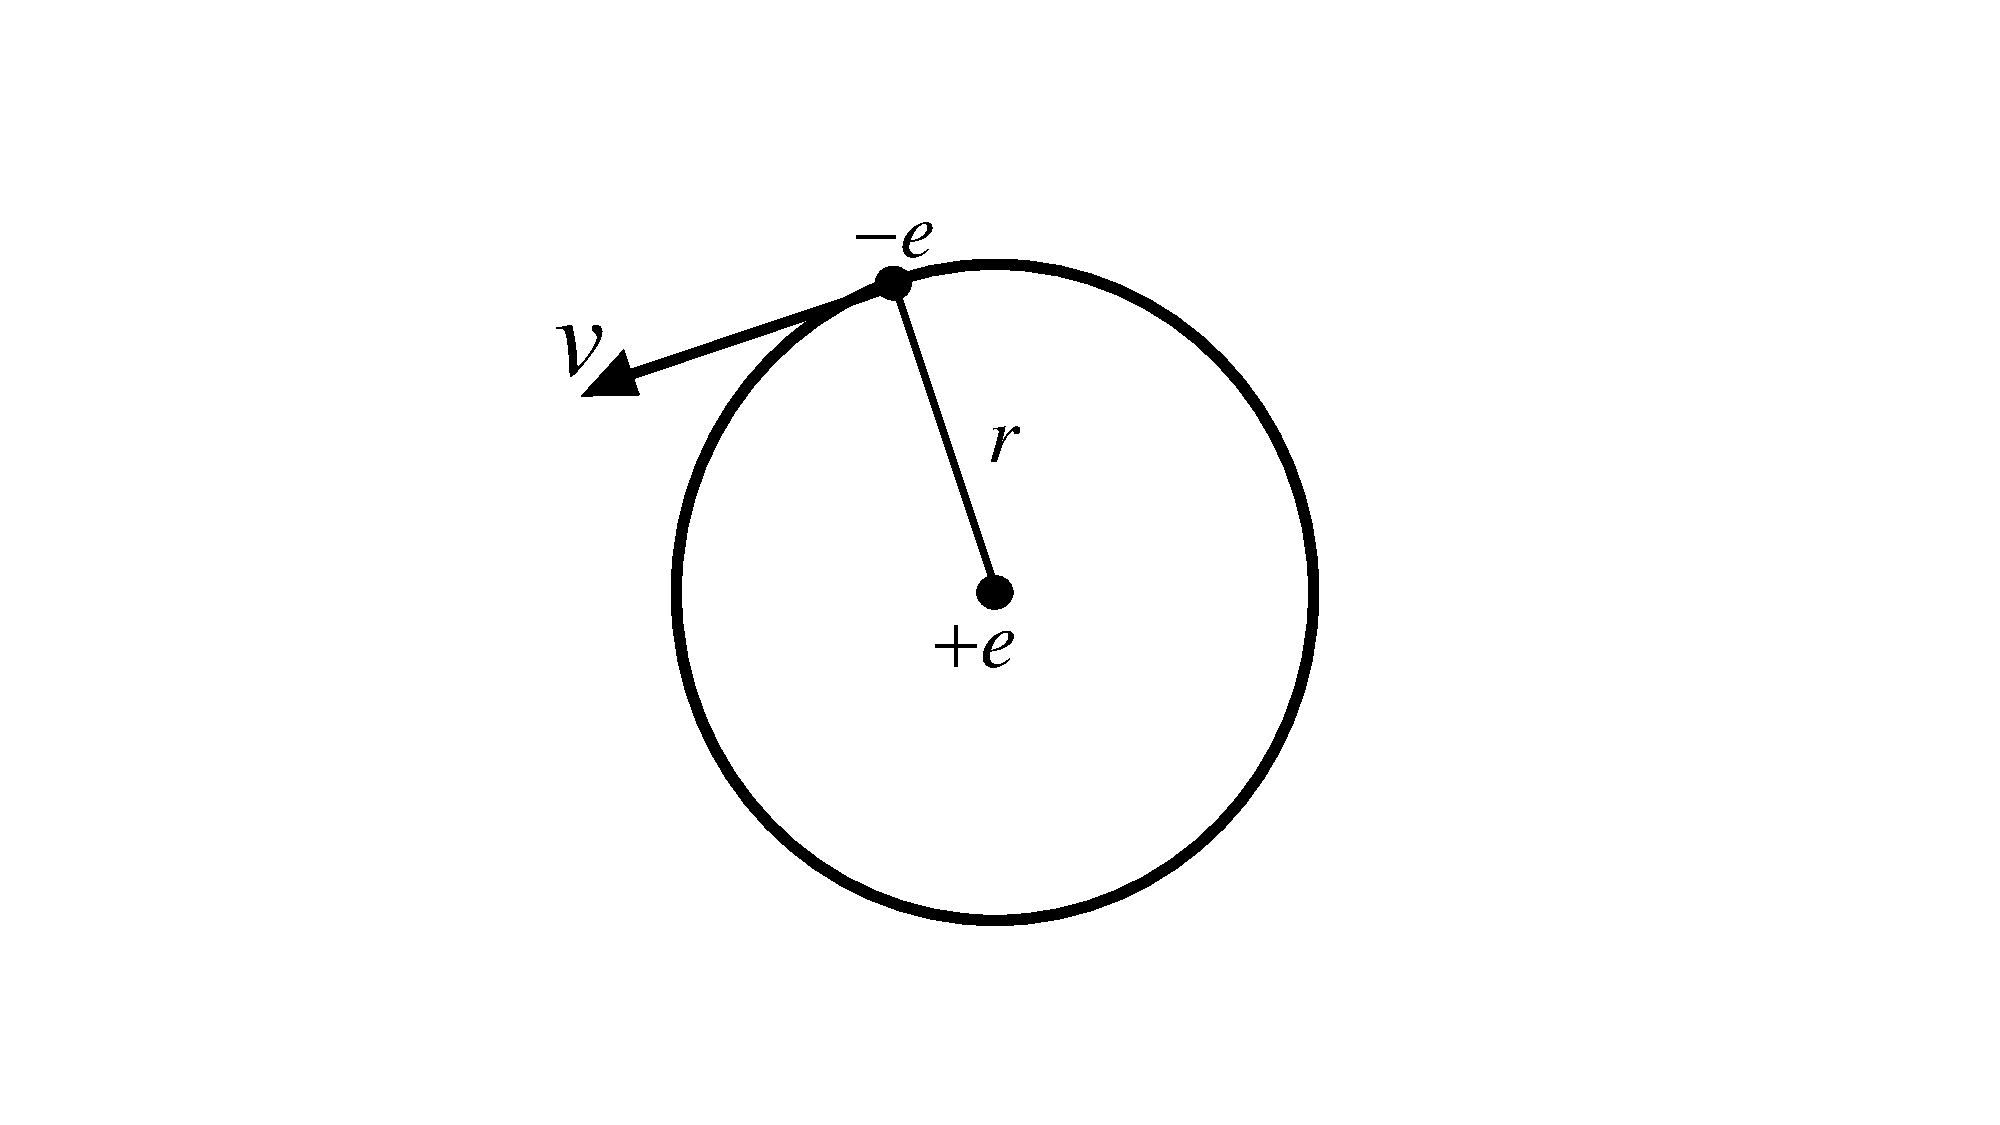
\includegraphics[width=2cm,clip]{QM file/figure/1-6}
	\caption{}
	\label{fig.1-6}
\end{wrapfigure}
后来,索末菲(Sommerfeld)将玻尔地量子化条件推广成为
\begin{equation}\label{eqn:01.03.11}
	\oint pdq =nh\quad n=1,2,3,\cdots
\end{equation}\eqshort
$p,q$为一对共轭地正则动量和坐标,$\oint$表示对运动的一个周期积分.推广后的量子化条件可以适用于任何周期性轨道,例如氢原子中电子的椭圆轨道.

玻尔认为,量子理论和经典物理理论之间并无不可逾越的鸿沟.量子理论概念适用于微观尺度,也适用于宏观尺度,经典理论仅适用于宏观尺度,在宏观尺度上,两种理论应该是一致的.这个观点成为对应原理.玻尔在20世纪20年代到各国宣讲他的量子理论时,强调对应原理是一个核心概念,而量子化条件则并不重要.下面我们根据对应原理对氢原子的能级和光谱试作分析.

考虑到圆轨道\ref{fig.1-6},电子的轨道半径r,速率v和角频率(角速度)$\omega$间的关系是
\begin{equation}\label{eqn:01.03.12}
	v=r\omega
\end{equation}
\eqnormal
原子核(电荷e)对电子的库伦吸引力就是圆周运动的向心力,
\begin{equation*}
	\frac{\e^{2}}{r^{2}}=m_{e}\frac{v^{2}}{r}=m_{e}r\omega^{2}
\end{equation*}\eqshort
因此
\begin{equation}\label{eqn:01.03.13}
	r^{3}\omega^{2}=\frac{\e^{2}}{m_{e}}
\end{equation}\eqnormal
电子运动的总能为
\begin{equation*}
	E=\frac{1}{2}m_{e}v^{2}-\frac{\e^{2}}{r}=\frac{1}{2}m_{e}r^{2}\omega^{2}-\frac{\e^{2}}{r}
\end{equation*}\eqshort
利用\eqref{eqn:01.03.13}式,得到
\begin{equation}\label{eqn:01.03.14}
	E=-\frac{\e^{2}}{2r}
\end{equation}\eqnormal
或
\begin{equation}\label{eqn:01.03.15}
	\omega=\bigg(\frac{8}{m_{e} \e^{4}}\bigg)^{\frac{1}{2}}(-E)^{\frac{3}{2}}
\end{equation}
\eqref{eqn:01.03.13}至\eqref{eqn:01.03.13}式适用于任何一条圆形轨道.以$n=1,2,3,\cdots$表示稳定轨道的序号,相应的$r,E,\omega$记为$r_{n},E_{n},\omega_{n}$,并规定$r_{n}$的编号次序为$r_1 < r_2 < r_3<\cdots$,当n不断增大,$r_{n}\rightarrow\infty$,$E_{n}\rightarrow 0^{-}$,所以$n\gg 1$相当于宏观尺度.

当电子由能级$E_{n}$跃迁到$E_{n-1}$,按照频率规则,发光角频率为
\begin{equation}\label{eqn:01.03.16}
	\omega=2\pi v=\frac{E_{n}-E_{n-1}}{\hbar}
\end{equation}
而按照电动力学,发光频率等于轨道运转频率,即$\omega_{n}$.按照对应原理,在$n\gg 1$时,$\omega$应该趋于$\omega_{n}$,即
\begin{equation}\label{eqn:01.03.17}
	E_{n}- E_{n-1}=\hbar\omega\rightarrow\hbar\omega_{n}
\end{equation}
亦即
\begin{equation}\label{eqn:01.03.18}
	E_{n}- E_{n-1}\rightarrow \bigg(\frac{8\hbar^{2}}{m_{e}\e^{4}}\bigg)^{\frac{1}{2}} (-E_{n})^{\frac{3}{2}},\quad n\gg 1
\end{equation}
$n\gg 1$时,n的变化($\Delta n=1$)远小于n本身,可以当作连续变化,因此
\begin{equation*}
	E_{n}- E_{n-1}=\Delta E_{n}
	=\frac{\Delta E_{n}}{\Delta n}\rightarrow\frac{dE_{n}}{dn}
\end{equation*}
\eqref{eqn:01.03.18}式可当作微分方程:
\begin{equation*}\label{eqn:01.03.18'}
	 \frac{dE_{n}}{dn}=
	 \bigg(\frac{8\hbar^{2}}{m_{e}\e^{4}}\bigg)^{\frac{1}{2}}(-E_{n})^{\frac{3}{2}},
	 \quad n\gg1		\tag{$1.3.18^{\prime}$}
\end{equation*}
容易解出
\begin{equation}\label{eqn:01.03.19}
	E_{n}=-\frac{1}{2n^{2}}\frac{m_{e}\e^{4}}{\hbar^{2}}=-\frac{1}{2n^{2}}\frac{\e^{2}}{a_{0}}
\end{equation}
再利用\eqref{eqn:01.03.14}式,得到
\begin{equation}\label{eqn:01.03.20}
	r_{n}=-\frac{\e^{2}}{2E_{n}}=n^{2}\frac{\hbar^{2}}{m_{e}\e^{2}}=n^{2}a_{0}
\end{equation}
其中$a_{o}=\frac{\hbar^{2}}{m_{e}\e^{2}}$为玻尔半径,即氢原子基态(n=1)半径.\eqref{eqn:01.03.19}、\eqref{eqn:01.03.20}式是在条件$n\gg 1$下得到的,如果认为这些结果也适用于n较小的情况,则它们就是氢原子能级和轨道半径的量子化公式.

以L表示轨道角动量,利用\eqref{eqn:01.03.13}及\eqref{eqn:01.03.20}式,容易得到
\begin{equation*}
	L^{2}=(m_{e}vr^{2})^{2}=m_{e}^{2}\omega^{2}r^{4}=m_{e}^{2}\frac{\e^{2}}{m_{e}}n^{2}\frac{\hbar^{2}}{m_{e}\e^{2}}=n^{2}\hbar^{2}
\end{equation*}
亦即
\begin{equation*}
	L=n\hbar,\quad n=1,2,3,\cdots
\end{equation*}
这正是量子化条件\eqref{eqn:01.03.10}.

当电子由能级跃迁但,按照频率规则\eqref{eqn:01.03.09},放光频率为
\begin{equation}\label{eqn:01.03.21}
	\nu_{nm}=\frac{E_{n}-E_{m}}{h}=2\pi^{2}\frac{m_{e}\e^{4}}{h^{3}}\bigg(\frac{1}{m^{2}} -\frac{1}{n^{2}}\bigg)
\end{equation}
和经验公式\eqref{eqn:01.03.02}比较,二者一致,并得里德伯(Rydberg)常数的结构式:
\begin{equation}\label{eqn:01.03.22}
	R=\frac{2\pi^{2}m_{e}\e^{4}}{ch^{3}}=\frac{m_{e}\e^{4}}{4\pi c\hbar^{3}}
\end{equation}
以各基本常数之值代入上式,得到R的理论值为$R=\num{109737}\si{cm^{-1}}$.严格地说,氢原子问题是二体问题,求电子能级时应该用折合质量$\mu=\frac{m_{e}m_{p}}{m_{e}+m_{p}}$代替以上计算中地电子质量$m_{e}$,这样得到的氢原子光谱里德伯常数理论值为
\begin{equation}\label{eqn:01.03.23}
	R_{H}=\frac{2\pi^{2}\mu \e^{4}}{ch^{3}}=\num{109677} \si{cm^{-1}}
\end{equation}
和实验值符合得极好.

\example 对于氢原子的第n个玻尔圆形轨道,求电子运行速度.

\solution 根据量子化条件\eqref{eqn:01.03.10}及轨道半径公式\eqref{eqn:01.03.20},易得速度公式:
\begin{equation*}
	v=\frac{n\hbar}{m_{e}r_{n}}=\frac{\hbar}{nm_{e}a_{0}}=\frac{\e^{2}}{n\hbar}=\frac{c}{n}\frac{\e^{2}}{\hbar c}
\end{equation*}\eqshort
其中$\frac{\e^{2}}{\hbar c}=\frac{1}{137}$,所以
\begin{equation}\label{eqn:01.03.24}
	v=\frac{c}{137}\cdot\frac{1}{n}
\end{equation}\eqnormal
按数量级而言,$v$约为光速的几百分之一,约为$10^{6}\si{m/s}$.


% 原子物理中的特征量
\section[原子物理中的特征量]{原子物理中的特征量}\label{sec:01.04}
% \makebox[5em][s]{} % 短题目拉间距
% \setlength{\mathindent}{9em} 本文标准公式缩进 
% \eqnormal % 恢复标准缩进


微观现象得普遍特点之一就是“量子化”,表征问题的各主要物理量常有一定的量级,它们和各个基本常数(常量)常有一定的构造关系.这种构造关系常可根据某些判据,利用量纲方法予以导出.

\textsf{1. 基本常数}

基本普适常数通常总是与某种基本物理规律相联系,例如玻耳兹曼常数K代表热平衡下的统计规律,光速c 表示相对论效应和电磁定律, 普朗克常数$\hbar$代表量子理论,元电荷e是电荷的量子化单位,等等.基本普适常数没有结构可言,它们表征着当今人类对客观物质世界的认识水平,它们的数值直接由实验决定.当问题涉及到某种基本粒子(例如电子)时,粒子的质量和自旋也是基本常数.
$\bigg($自旋总是$\hbar$的$\frac{n}{2}$倍,$n=0,1,2,\cdots$,通常可以不必另行作为基本常数提出. $\bigg)$

由于库仑定律的表现形式为$F=-\frac{e_{1}e_{2}}{r^{2}}$,所以$e^{2}$具有(能量)$\times$(长度)的量纲,和$\hbar c$的量纲相同,因此$\frac{e^{2}}{\hbar c}$是无量纲普适常数,它表征着基本电荷间的电磁作用.历史上它是在研究原子光谱的精细结构时被发现的,故称精细结构常数,其数值为
\begin{equation*}
	\frac{\e}{\hbar c}\bigg(\text{即}\frac{1}{4\pi\varepsilon_{0}}\frac{e}{\hbar c} \bigg)=\num{7.29335}\times10^{-3} \approx \frac{1}{137}
\end{equation*}
这是一个十分重要的普适常数,有些量纲相同的特征量之间的相互关系常可通过精细结构常数表示出来.

\textsf{2. 原子能级}

电子的相对论静能为$m_{e}c^{2}=0.51 \si{MeV}$.研究电子运动时,如果能量变化远小于$m_{e}c^{2}$,为低速运动,这时原则上可以不用相对论理论.如能量的变化接近或超过$m_{e}c^{2}$,为高速运动,即高能范围,必须用相对论理论.

根据实验测定,原子的(外层)电子能级,量级约10 \si{eV}, 远小于$m_{e}c^{2}$,属于非相对论范围.由于电荷间的库仑力也与c无关,所以可以断定原子的电子能级公式中不会出现光速c.利用这个判据, 易知电子能级的特征值(不包括静能$m_{e}c^{2}$)必为
\begin{equation}\label{eq14.1}
	\begin{aligned}
		E &\sim m_{e}c^{2}\bigg(\frac{\e}{\hbar c} \bigg)^{2}= \frac{m_{e}e^{4}}{\hbar^{2}} \\
		&\sim \num{0.511}\times10^{6}\si{eV}\times\bigg(\frac{1}{137} \bigg)^{2}\sim \num{27.2}\si{eV}
	\end{aligned}
\end{equation}\eqshort

\textsf{3. 特征长度}

上述电子能级特征值可以写成
\begin{equation}\label{eq14.2}
	E\sim \frac{\e^{2}}{a_{0}}
\end{equation}\eqnormal
其中
\begin{equation}\label{eq14.3}
	a_{0}=\frac{\hbar^{2}}{m_{e}\e^{2}}-\num{0.53}\times 10^{-10}\si{m}
\end{equation}\eqshort
是原子结构的特征长度,即玻尔半径.它是量子论的(含有$\hbar$),又是非相对论的(与c无关).

原子光谱的波长$\lambda=\frac{c}{\nu}$,$\nu$为频率.根据玻尔量子论[见\eqref{eqn:01.03.09}式],$\nu=\frac{E_{n}-E_{n^{\prime}}}{h}$所以
\begin{equation}\label{eq14.4}
	\lambda=\frac{hc}{E_{n}-E_{n^{\prime}}}
\end{equation}
能级差($E_{n}-E_{n^{\prime}}$)一般为几个\si{eV},而hc的值为
\begin{equation*}
	hc=1.24\times10^{-6} \si{eV\cdot m}
\end{equation*}\eqlong
所以$\lambda$一般为$10^{2}\sim10^{3} \si{nm}$量级.例如当($E_{n}-E_{n^{\prime}}$)= =2 \si{eV},$\lambda$=620 \si{nm} ,属于可见光范围.

玻尔半径$a_{0}$和精细结构常数相乘,即得电子的约化康普顿波长:
\begin{equation}\label{eq14.5}
	\lambdabar_{c}=a_{0}\bigg(\frac{\e}{\hbar c} \bigg)=\frac{\hbar}{m_{e}c}\sim\frac{a_{0}}{137}\sim3.86\times10^{-13}\si{m}
\end{equation}\eqnormal
原始的康普顿波长(见\ref{sec:01.02})是指
\begin{equation}\label{eq14.6}
	\lambda_{c}=\frac{h}{m_{e}c}\sim2.43\times10^{-12} \si{m}
\end{equation}
康普顿波长与$h,c$及粒子质量有关(但与电荷无关),故凡相对论和量子论同时起决定性作用的现象中,特征长度通常就是康普顿波长.例如(电子、正电子)对的产生或湮没,就在康普顿波长的范围内发生. 又如核力(强作用)的传递是与$\pi$介子的产生和湮没相联系的,但与电磁作用无关,因此核力的力程必为$\pi$介子的康普顿波长的量级,即
\begin{equation}\label{eq14.7}
	\text{核力力程} \sim\frac{\hbar}{m_{\pi}c} \sim\frac{\lambdabar_{c}}{270}\sim 1.4\si{fm}
\end{equation}
($m_{\pi}\sim 270 m_{e}$),这与核力力程的公认实验值(约2 \si{fm}左右)是一致的.

有关电子运动的另一个更小的特征长度是电子经典半径:
\begin{equation}\label{eq14.8}
	r_{e}=\lambdabar_{e}\bigg(\frac{\e}{\hbar c} \bigg)=\frac{\e^{2}}{m_{e}c^2}\sim 2.8 \si{fm}
\end{equation}
它与量子论无关(与h 无关),故称“经典半径”.其实电子的真实“半径”远小于$10^{3} \si{fm}$. 现今在前沿理论中,电子通常当作点电荷对待.

\textsf{4. 速度和角速度}

原子中电子的运动属于低能范围,电子速度v的公式应该与c无关,因此可以断定
\begin{equation}\label{eq14.9}
	v\sim c \cdot\frac{\e}{\hbar c}=\frac{\e^{2}}{\hbar}\sim\frac{c}{137}
\end{equation}
也可以利用能级特征值公式\eqref{eq14.1},并利用$E\sim m_{e}v^{2}$得出\eqref{eq14.9}式.上式大致表征了外层电子(价电子)的速度.在原子的最内层,电子所受作用力大体上就是直接来自原子核(电荷$Ze$,$Z$为原子序数)的未经其他电子屏蔽的库仑力,$F\sim\frac{Z\e^{2}}{r^{2}}$,这时\eqref{eq14.1}式和\eqref{eq14.9}式中$\e^{2}$应换成$Z\e^{2}$,因此$v\sim\frac{cZ}{137}$,当Z较大时,v可达光速c的一半以上.这种情况下应该用相对论量子力学来描写电子的运动.

电子沿基态玻尔轨道(n = 1)运动时,角速度为
\begin{equation}\label{eq14.10}
	\omega_{1}=\frac{v}{a}\sim\frac{1}{137}\frac{c}{a_{0}}4.1\times10^{16} \si{s^{-1}}
\end{equation}\eqshort
沿量子数为n的圆轨道运动时,由$\S$\ref{sec:01.03}\eqref{eqn:01.03.13},\eqref{eqn:01.03.20}式,可得角速度为
\begin{equation}\label{eq14.11}
	\omega_{n}=\frac{\omega_{1}}{n^{3}}
\end{equation}\eqnormal
电子的轨道周期为$\frac{2\pi}{\omega}$,对于第n个玻尔圆轨道,周期为
\begin{equation}\label{eq14.12}
	\frac{2\pi}{\omega_{n}}=n^{3}\frac{2\pi}{\omega_{1}}=\frac{2\pi n^{3}\hbar^{3}}{m_{e}\e^{4}}
\end{equation}\eqlong
其中
\begin{equation}\label{eq14.13}
	\frac{2\pi}{\omega_{1}}=2\pi\frac{\hbar}{m_{e}\e^{4}}=2\pi\times137\frac{a_{0}}{c}\sim1.5\times10^{-16} \si{s}
\end{equation}\eqnormal

\textsf{5. 电矩和磁矩}

原子的内层电子大致呈球对称分布,对电矩和磁矩无贡献,原子的电矩和磁矩主要来自外层电子.以氢原子为例,电偶极矩约为
\begin{equation}\label{eq14.14}
	D\sim er\sim ea_{0}=\frac{\hbar^{2}}{m_{e}\e}\quad(n=1)
\end{equation}

电子沿圆形轨道匀速运动时,相当于一个环形电流,环的面积为$A=\pi r^{3}$,电流为$I=-\frac{\e\omega}{2\pi}$.按照电磁理论,这种环形电流的等效磁矩为
\begin{equation}\label{eq14.15}
	\begin{aligned}
		\mu=IA=-\frac{\e r^{2}\omega}{2} \text{(国际单位制)} \\
		\mu=\frac{IA}{c}=-\frac{\e r^{2}\omega}{2c} \text{(高斯单位制)}
	\end{aligned}
\end{equation}
电子的轨道角动量为$L=m_{e}vr=m_{e}r^{2}\omega$,所以磁矩和角动量的关系为
\begin{equation}\label{eq14.16}
	\begin{aligned}
		\boldsymbol{\mu}&=-\frac{\e}{2m_{e}}\boldsymbol{L} \text{(国际单位制)} \\
		\boldsymbol{\mu}&=-\frac{\e}{2m_{e}c}\boldsymbol{L} \text{(高斯单位制)}
	\end{aligned}
\end{equation}
由于电子电荷为负,轨道角动量$\boldsymbol{L}$的方向和磁矩$\mu$的方向相反.容易证明,\eqref{eq14.16}式也适用于椭圆轨道.按照玻尔的量子化条件,角动量L 是量子化的,其单元为$\hbar$,因此磁矩$\mu$也是量子化的,其单元为“玻尔磁子”:
\begin{equation}\label{eq14.17}
	\begin{aligned}
		\mu_{B}&=-\frac{\e\hbar}{2m_{e}} \text{(国际单位制)} \\
		\mu_{B}&=-\frac{\e\hbar}{2m_{e}c} \text{(高斯单位制)}
	\end{aligned}
\end{equation}\eqshort
国际单位制中,电矩与磁矩量纲不同在高斯单位制中,电矩与磁矩量纲相同,比值约为
\begin{equation}\label{eq14.18}
	\frac{\mu}{D}\sim\frac{\e^{2}}{\hbar c}\sim\frac{1}{137}
\end{equation}

\textsf{6. 经典电偶极矩振子的辐射功率}

具有确定频率$\nu=\frac{\omega}{2\pi}$的电偶极矩振子,其电偶极矩为
\begin{equation}\label{eq14.19}
	D(t)=D\cos\omega t
\end{equation}
按照经典电动力学理论,这个偶极矩振子将向外辐射同样频率的电磁波,总辐射功率为
\begin{equation}\label{eq14.20}
	-\frac{dE}{dt}=\frac{D^{2}\omega^{4}}{3c^{3}}
\end{equation}
电子以角速度$\omega$沿半径为r的圆周运动时,相当于两个振动方向互相垂直的电偶极矩振子($D = er$),按照电动力学,其总辐射功率为
\begin{equation}\label{eq14.21}
	-\frac{dE}{dt}=\frac{2}{3}\frac{\e^{2}r^{2}\omega^{4}}{c^{3}}
\end{equation}\eqnormal
在这里我们用虽纲方法对这两个公式作一些说明.如果偶极振子确实存在电磁辐射,其总辐射功率显然取决于电偶极矩振幅D,角频率$\omega$以及光速c(来自麦克斯韦方程).它们的量纲为
\begin{gather} 
	c—— \si{LT^{-1}},\quad \omega—— \si{T^{-1}},\quad \frac{c}{\omega}—— \si{L} \notag\\
	\frac{dE}{dt}—— \si{ET^{-1}}.\quad D^{2}—— \e^{2}r^{2}—— \si{EL^{3}} \notag
\end{gather}\eqshort
因此,辐射功率唯一可能的量纲构造方式为
\begin{equation}\label{eq14.22}
	-\frac{dE}{dt}\sim\frac{D^{2}\omega^{4}}{c^{3}}
\end{equation}\eqnormal
它和电动力学的严格计算结果\eqref{eq14.20}、\eqref{eq14.21}式只相差一个量级为1的纯数值系数.

\textsf{7. 原子激发态的平均寿命}

按照玻尔量子论,原子中的电子停留在某个能级(稳定轨道)上时,并不辐射电磁波;当电子由某个较高能级跃迁到较低能级时,将辐射电磁波(光子).实验发现,对于一个原子,这种能级跃迁是突变式的, 但带有概率性,大最处于相同能级的原子,它们的能级跃迁并非同时发生,而是大体上在某段时间$\tau$内完成,$\tau$称为初始能级的平均寿命.利用对应原理分析能级跃迁过程得到的结论是,原子能级跃迁过程的电磁辐射性质,相当于经典电偶极矩振子.以氢原子中电子由能级$E_{2}$跃迁到$E_{1}$为例,跃迁过程释放出的总能量为($E_{2}-E_{1}$),辐射角频率为$\omega=\frac{E_{2}-E_{1}}{\hbar}$,相应的电偶极矩振幅可以估计为$\sim ea_{0}$,因此辐射功率约为
\begin{equation*}
	-\frac{dE}{dt}\sim\frac{D^{2}\omega^{4}}{c^{3}}\sim
	\frac{\e^{2}a_{0}^{2}(E_{2}-E_{1})^{4}}{c^{3}\hbar^{4}}
\end{equation*}
因此电子停留在激发态能级($E_{2}$)的平均寿命约为
\begin{equation}\label{eq14.23}
	\tau\sim\frac{E_{2}-E_{1}}{|\frac{dE}{dt}|}\sim
	\frac{c^{3}\hbar^{4}}{\e^{2}a_{0}^{2}(E_{2}-E_{1})^{3}}
\end{equation}
由$\S$\ref{sec:01.03}\eqref{eqn:01.03.19}式
\begin{equation*}
	E_{2}-E_{1}=\frac{3}{8}\frac{\e^{2}}{a_{0}}=\frac{3}{8}\frac{m_{e}\e^{4}}{\hbar^{2}}\sim10.2\si{eV}
\end{equation*}
代入\eqref{eq14.23}式,得到
\eqlong
\begin{equation}\label{eq14.24}
	\begin{aligned}
		\tau &\sim \bigg(\frac{8}{3} \bigg)^{3} \bigg(\frac{\hbar c}{\e^{2}} \bigg)^{4} \frac{a_{0}}{c}  \\
		&\sim \bigg(\frac{8}{3} \bigg)^{3} (137)^{4} \frac{0.53\times10^{-10}}{3\times10^{8}}\si{s} \approx1.2\times10^{-9}\si{s}
	\end{aligned}
\end{equation}
扯子力学的精确计算结果为(见$\S 9.4$)%(见$\S$\ref{sec:09.04})
\begin{equation}\label{eq14.25}
	\tau_{2p\rightarrow 1s}=
	\bigg(\frac{3}{2} \bigg)^{8} \bigg(\frac{\hbar c}{\e^{2}} \bigg)^{4} \frac{a_{0}}{c}=1.6\times10^{-9} \si{s}
\end{equation}\eqnormal
注意,电子在$E_{2}$能级上的轨道运动周期为[见\eqref{eq14.12}、\eqref{eq14.13}式]
\begin{equation*}
	\frac{2\pi}{\omega_{2}}\sim1.2\times10^{-15} \si{s}
\end{equation*}
处于$E_{2}$轨道上的电子,在跃迁到$E_{1}$轨道之前,在$E_{2}$轨道上的平均运行圈数约为
\begin{equation*}
	\frac{\tau\omega_{2}}{2\pi}\sim \frac{32}{27\pi} \bigg(\frac{\hbar c}{\e^{2}} \bigg)
	\sim 10^{6}
\end{equation*}
“稳定轨道”的意义于此可见一斑.

\eqref{eq14.23}式大致可以适用于其他单价原子的价电子光学跃迁,只是其中$a_{0}$应改为原子半径的实际数值.例如取原子半径$a_{0}\sim0.1 \si{nm}$,当$(E_{2}-E_{1})\sim 2\si{eV}$(发射光波波长$\lambda \sim620 \si{nm}$) ,激发态平均寿命$\tau\sim4.5\times10^{-8}\si{s}$.





% 德布罗意的“物质波”假设
\section[德布罗意的“物质波”假设]{德布罗意的“物质波”假设}\label{sec:01.05}
% \makebox[5em][s]{} % 短题目拉间距
% \setlength{\mathindent}{9em} 本文标准公式缩进 
% \eqnormal % 恢复标准缩进

玻尔量子论的建立,极大地推动了原子物理学的发展.但随着研究的深入,玻尔量子论的局限性也逐渐暴露出来.例如任何一种原子光谱,各条谱线的相对强度表现出很好的规律性,玻尔量子论未能对此作出满意的解释.氨原子光谱表现出某些奇特的规律(似乎是由两套光谱混杂而成),玻尔量子论对此也无力解释长期以来,许多化学和物理理论中,从来认为原子的形状像一个小球,这个概念早已被多种实验事实所肯定. 但在玻尔量子论中,电子作平面轨道运动,因此原子(尤其是氢原子)的形状更像一个饼.

1924年,德布罗意提出了“物质波” 的假设.德布罗意注意到了几何光学(光的宏观传播规律)和质点力学有着惊人的相似性.光在均匀介质中沿直线传播的定律,在两种介质的分界面处光的反射和折射定律,以及在不均匀介质中光沿曲线传播的规律,可以统一为“最小光程原理(费马原理)”, 即
\eqshort
\begin{equation}\label{eq15.1}
	\delta\int_{A}^{B} ndl = 0
\end{equation}\eqnormal
光由A点传播到B点,$\int_{A}^{B}\cdots dl$表示由A到B的线积分,n为折射率,(A,B)间任何一条可能的路径的光程即$\int_{A}^{B}ndl$,光程最小的路径就是实际的光线.牛顿质点力学定律可以表示成“最小作用量原理”,即
\begin{equation}\label{eq15.2}
	\delta\int_{A}^{B}pdl=\delta\int_{A}^{B}\sqrt{2m(E\sim V)}dl
\end{equation}\eqlong
\begin{wrapfigure}[5]{r}{8em}
	\centering
	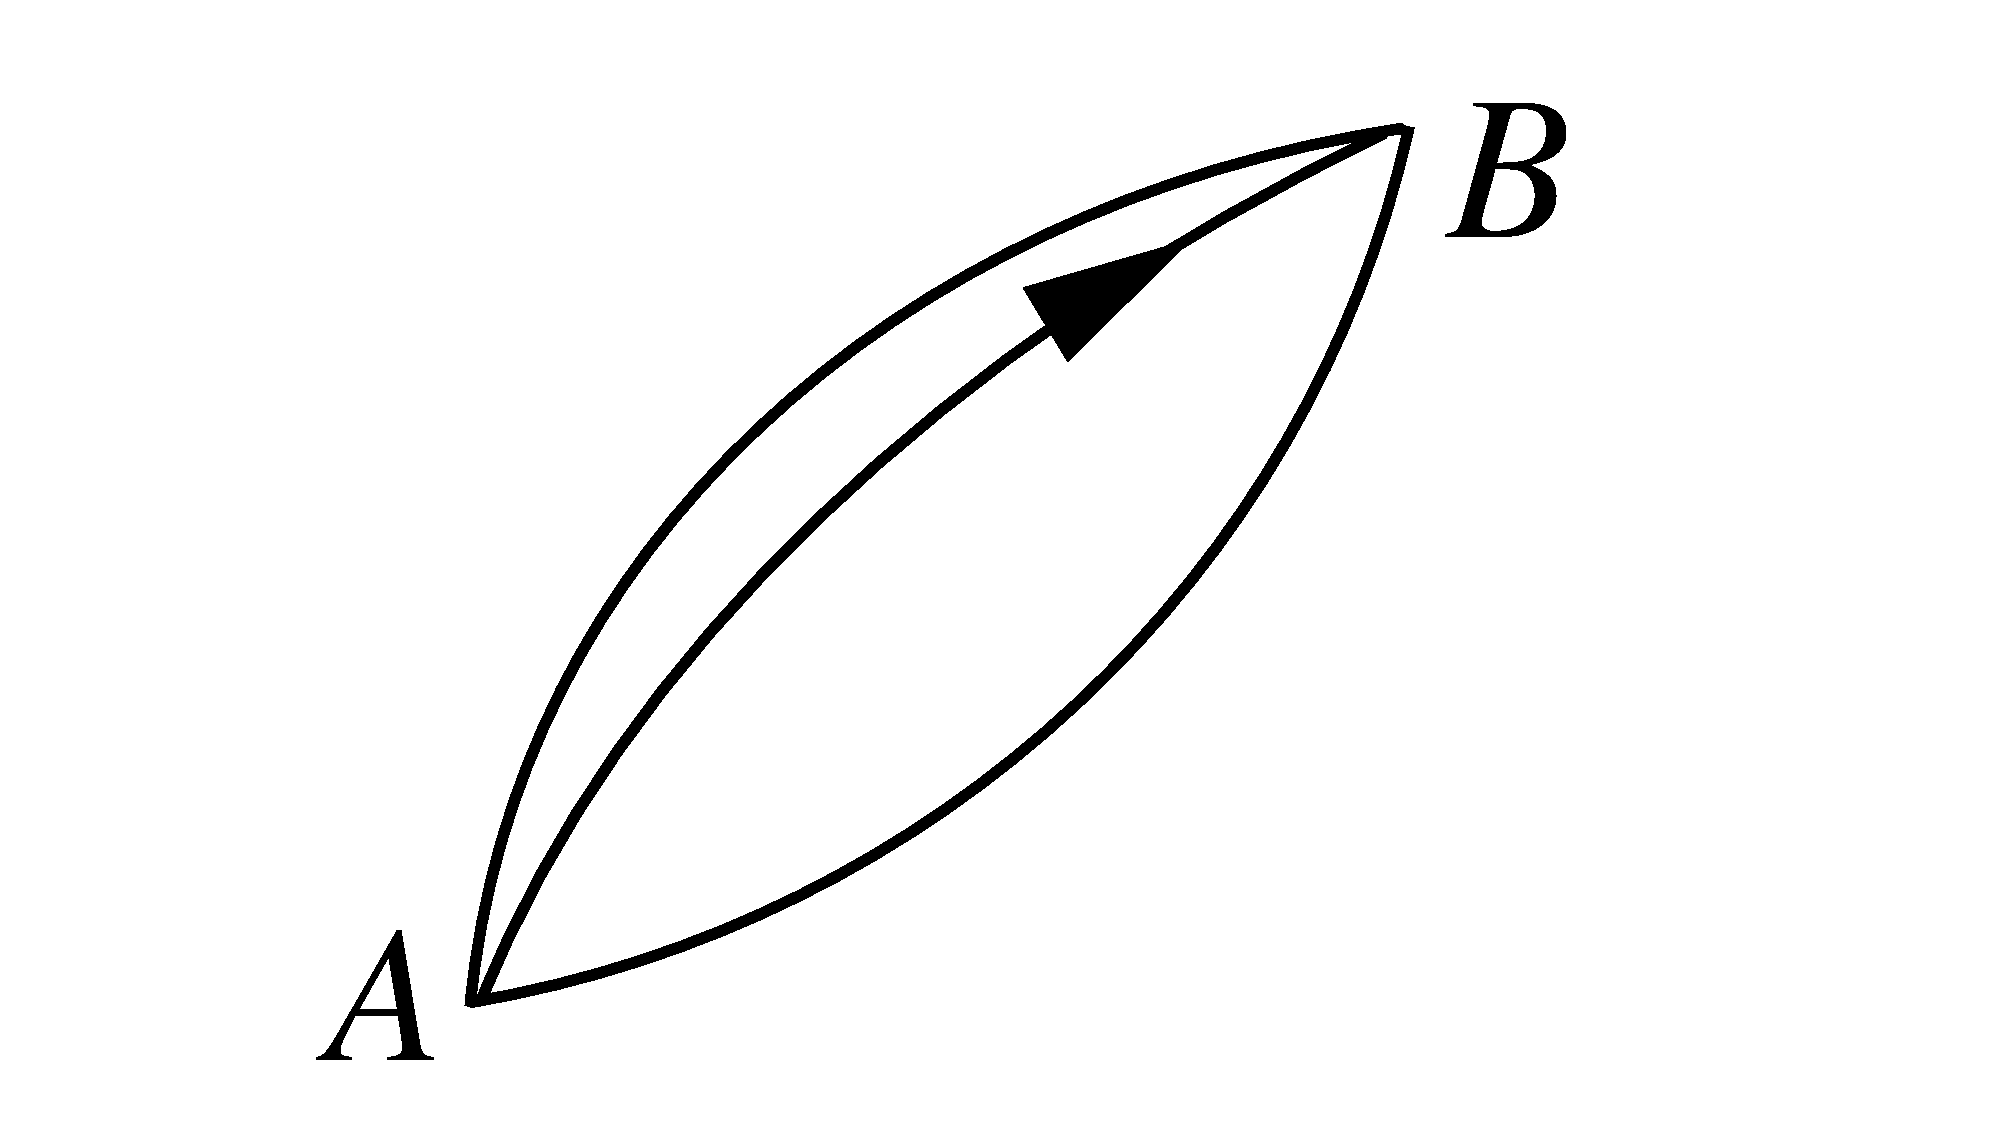
\includegraphics[width=2.5cm,clip]{QM file/figure/1-7}
	\caption{}
	\label{fig.1-7}
\end{wrapfigure}
其$m,p,E,V$表示质点的质量,动量,总能和势能,$\int pdl$称为作用量,质点由A至B的实际路径是作用量最小的路径.

德布罗意注意到光的本质包含者粒子和波动两个方面,光具有量子化的结构,每个光子具有一定的能量和动量:
\begin{equation}\label{eq15.3}
	E=\hbar\omega,\quad p=\frac{h}{\lambda},\quad \boldsymbol{p}=\hbar\boldsymbol{k}\quad
	(k=\frac{2\pi}{\lambda})
\end{equation}\eqnormal
在传播过程中,光表现出波动性,干涉、衍射等现象就是波动性的典型特征.但在宏观尺度上光的传播可以用光线概念来表述,波动光学表现为几何光学,波动规律以类似于力学规律的形式表现出来.德布罗意认为,电子以及其他物质粒子也都应该具有波动$\sim$粒子二重性.电子在结构上的量子性已为汤姆孙荷质比实验(测量$\frac{e}{m_{e}}$)所证实,电子在宏观尺度的运动遵守牛顿质点力学的规律,这早已被实验肯定.德布罗意认为,电子运动规律本质上应该是波动规律,这种波动性只有在微观尺度(量级和波长接近的尺度)才能表现出来,而在宏观尺度则表现为牛顿力学规律.德布罗意认为爱因斯坦公式\eqref{eq15.3}也适用于一切物质粒子,它们的力学性质$(E,p)$和波动性质$(\omega,\lambda)$通过普朗克常数$\hbar$互相联系.
\begin{wrapfigure}[8]{r}{8em}
	\centering
	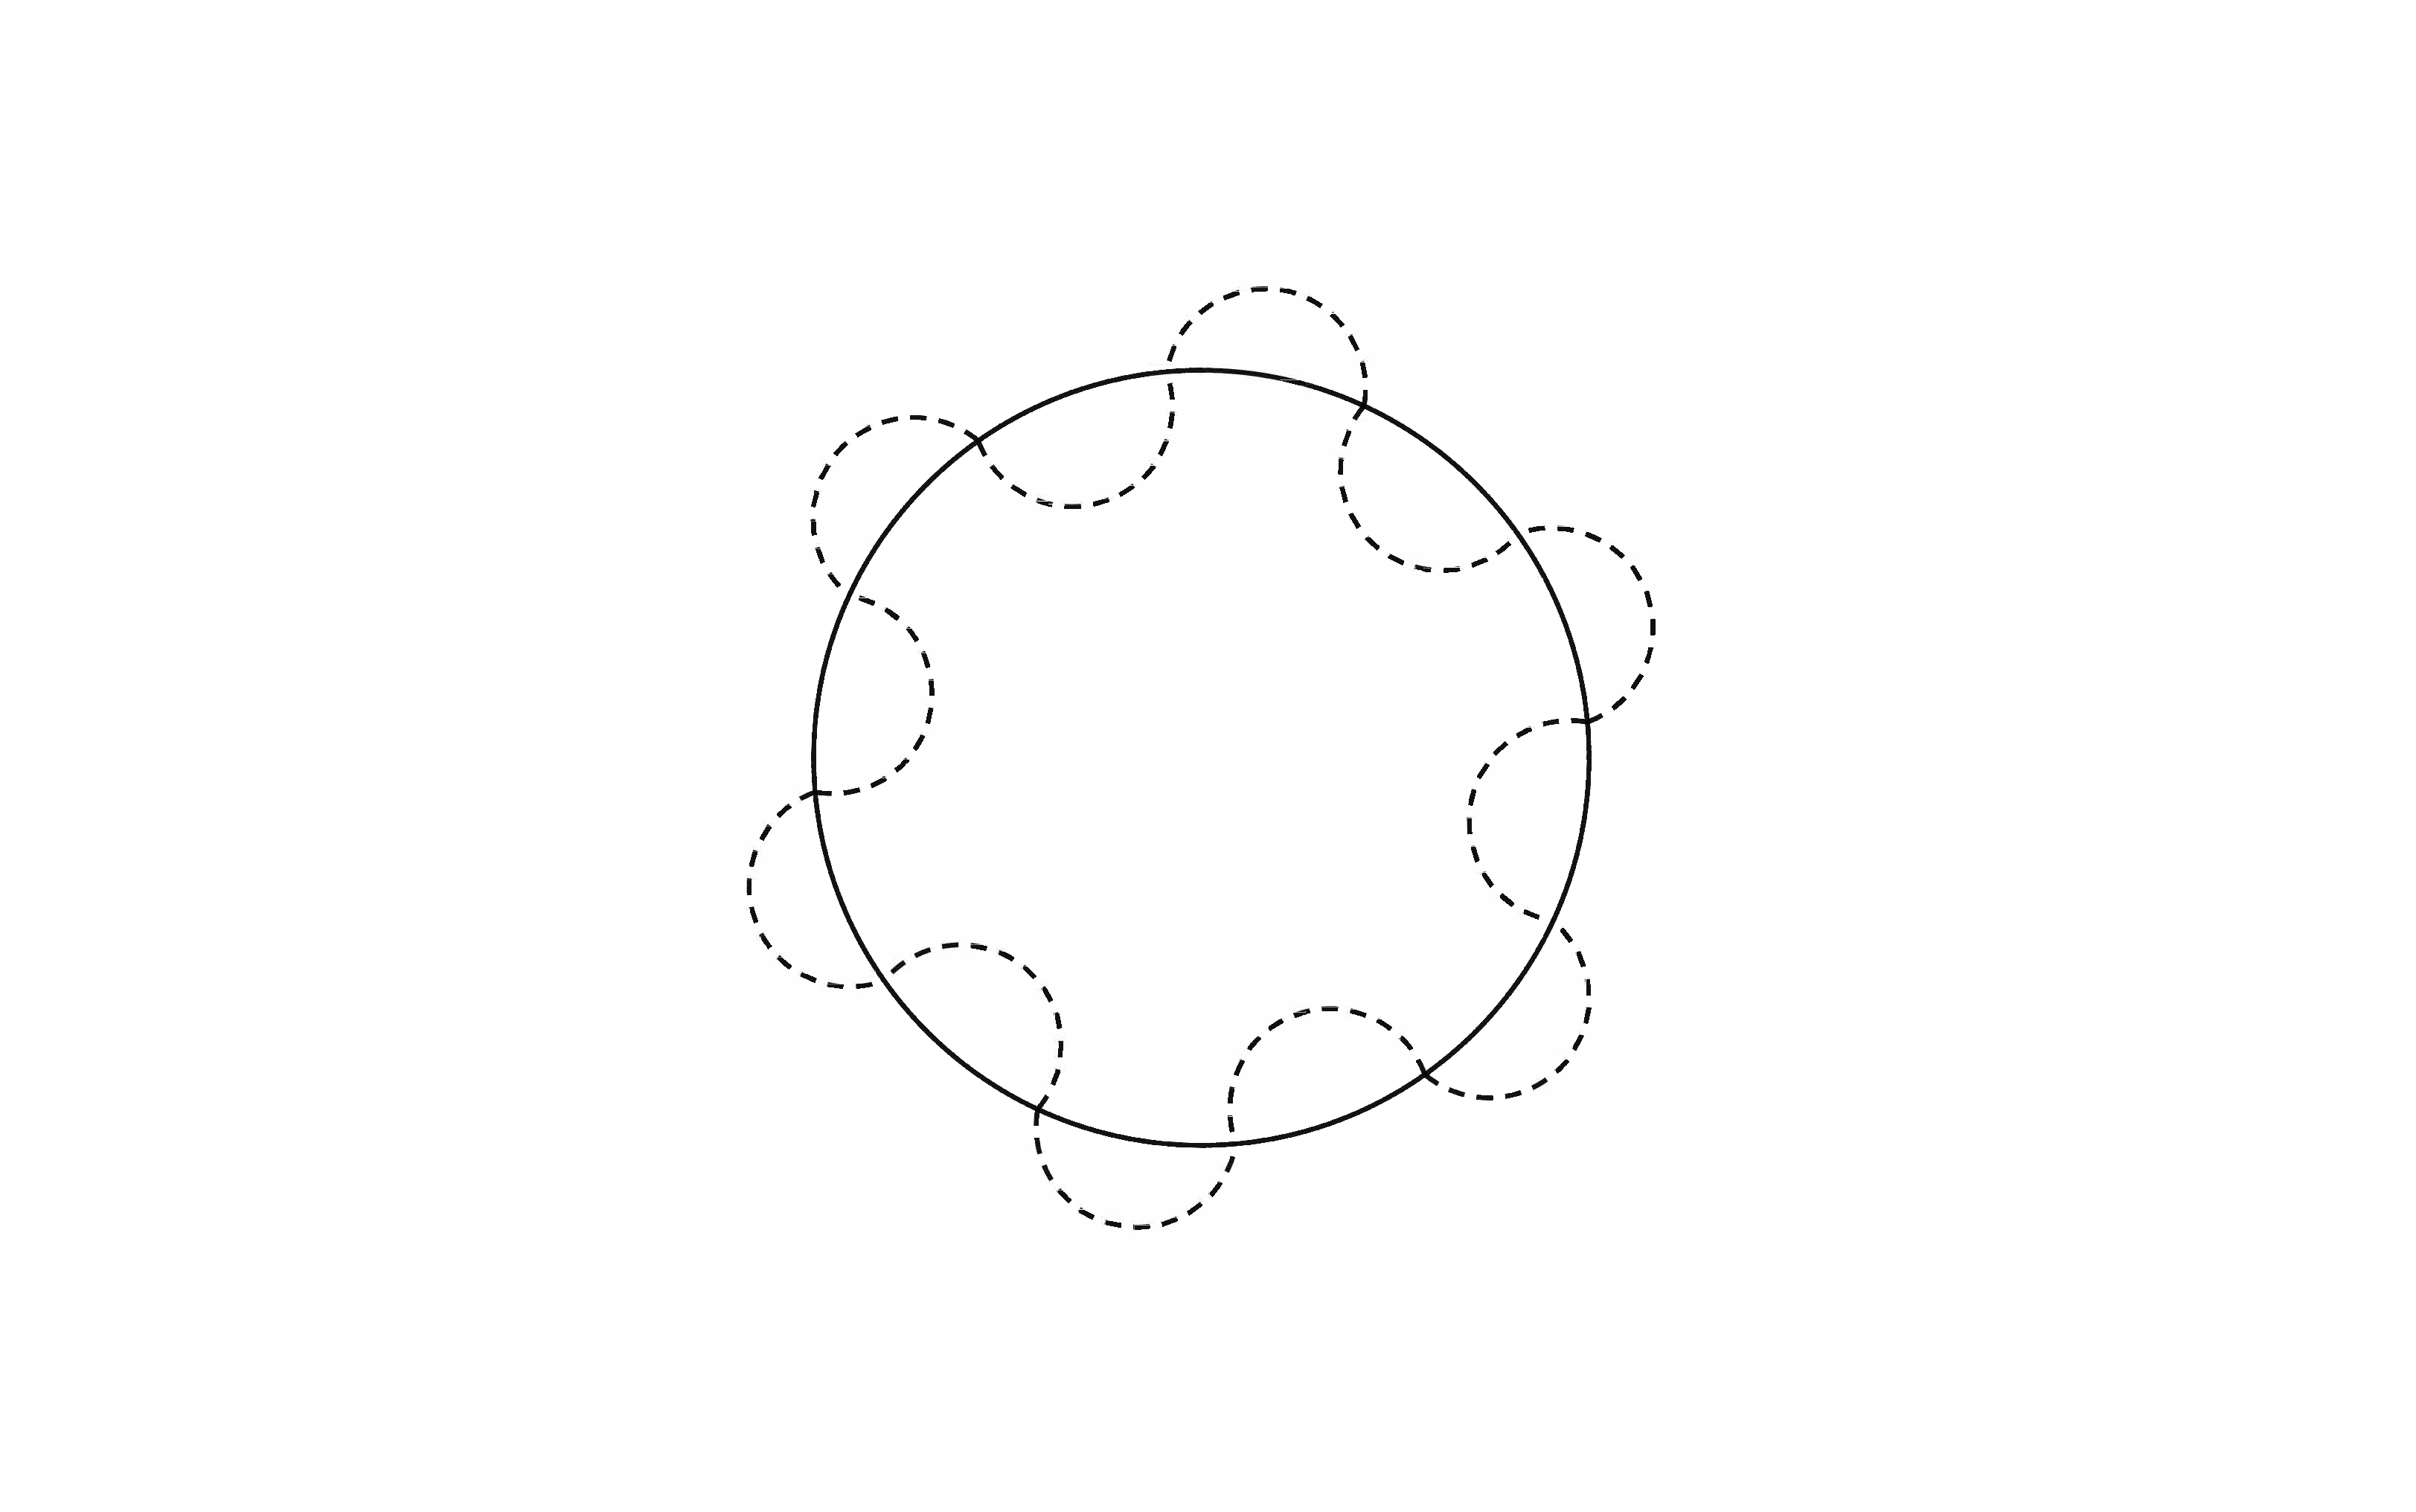
\includegraphics[width=2.5cm,clip]{QM file/figure/1-8}
	\caption{}
	\label{fig.1-8}
\end{wrapfigure}

德布罗意提出上述“物质波”设想时,并无直接的实验根据,而是一种科学假设.他希望这种未经证实的电子的波动性能够解释玻尔量子论所无法解释的那些困难问题.他指出,玻尔量子论中的量子化条件(这是玻尔理论中最难理解的一条)的实质很容易用波动的观点给以解释,如下.电子沿轨道运动,相当于物质波沿轨道传播,如果轨道周长不等于波长的整数倍,物质波将自行干涉而消失,亦即这种轨道是不允许的;如果轨道周长等于波长的整数倍,则物质波就能形成谐波而稳定存在,相应的轨道为稳定轨道形成谐波的条件为
\begin{equation}\label{eq15.4}
	\oint\frac{dq}{\lambda}=n,\quad n=1,2,3,\cdots	
\end{equation}
以$\lambda=\frac{h}{p}$代入上式,即得
\begin{equation}\label{eq15.5}
	\oint pdq=nh,\quad n=1,2,3,\cdots
\end{equation}
这正是量子化条件.

德布罗意的物质波思想直接导致了量子力学的诞生.相隔不到2年,薛定谔(E.Schr\"{o}dinger)就以“波动力学”的形式建立了量子力学(1926).稍早几个月,海森伯(W.Heisenberg)以“矩阵力学”的形式建立了量子力学(1925).

1927 年正式做了电子衍射实验,证实了电子确实具有波动性.接着又做了中子衍射实验,各种原子束和分子束的衍射实验,20世纪90年代还做了$C_{60}$分子(由60个碳原子形成的足球状大分子)束衍射实验,这些实验无一例外地都证实了公式$p=\frac{h}{\lambda}$的正确性,证实了实物粒子确实具有波动性.

当实物粒子在某种尺度的空间范围内运动时,如相应的物质波波长远小于空间尺度,一般可以不考虑粒子的波动性,而用经典力学处理粒子的运动.如波长接近或大于空间尺度,则波动性表现为粒子运动规律的主要方面,这时必须用量子力学来处理粒子的运动.下面举几个典型例子.

(1)气体分子的热运动.温度T下气体分子的热运动(平移)动能为$\frac{3kT}{2}$,$T=300 \si{K}$(室温)时,分子动能约为\num{0.039}\si{eV},相应的物质波波长为
\begin{equation*}
	\lambda=\frac{h}{p}=\frac{hc}{\sqrt{2m_{\text{分子}}\times\num{0.039}\si{eV}}}
\end{equation*}\eqshort
对于氧分子($O_{2}$),$m_{O_{2}}\approx32m_{p}\approx32\times938\times10^{6}\si{eV/c^{2}}$,波长$\lambda\approx0.026\si{nm}$,远小于分子的平均自由程,所以分子的热运动可作经典力学处理.

(2)原子中的电子运动电子动能的量级约10\si{eV},容易求得波长的量级为
\begin{equation*}
	\lambda\sim\frac{hc}{\sqrt{2m_{e}c^{2}E}}\sim 0.39\si{nm}
\end{equation*}\eqnormal
$\frac{\lambda}{2\pi}$和原子半径量级(0.1\si{nm})相同,所以要用量子力学来处理.

氢原子的基态,电子动能和动量为
\begin{equation*}
	\frac{p^{2}}{2m_{e}}=\frac{\e^{2}}{2a_{0}},\quad \boldsymbol{p}=\sqrt{\frac{m_{e}\e^{2}}{a_{0}}}=\frac{m_{e}\e^{2}}{\hbar}=\frac{\hbar}{a_{0}}
\end{equation*}\eqshort
波长为
\begin{equation*}
	\lambda=\frac{h}{p}=2\pi a_{0}
\end{equation*}\eqnormal
$a_{0}$为玻尔半径.

(3)原子核中核子的运动.核子(质子和中子)的动能约为$E\sim20 \si{MeV}$,相应的波长约为

\begin{equation}
	\begin{aligned}
		\lambda &\sim \frac{hc}{\sqrt{2m_{p}c^{2}E}}	\notag \\
				&\sim \frac{1.24\times10^{3} \si{MeV\cdot fm}}{\sqrt{2\times938\times20(\si{MeV})^{2}}}
				\approx 6.4 \si{fm}. \notag
	\end{aligned}
\end{equation}
核子的物质波波长$\lambda$和原子核半径同数量级,所以核子的运动也要用量子力学来处理.

% 习题
\begin{exercises}

\exercise 远离恒星的宇宙空间充满了温度$T=2.8\si{K}$的热辐射(称为宇宙背景辐射),这是宇宙发展早期“大爆炸"的遗迹. 试估算这种“背景辐射”的光子数密度.

\exercise 在宇宙发展的早期,温度极高,热辐射光子互相碰撞,可以转变成一对正负电子.试估算当时温度的量级.

\exercise 对于光子被自由电子散射(康普锁散射)问题,设光子能量远小于$m_{e}c^{2}$,则散射过程中电子的能量、动量变化可以用牛顿力学处理.试作出相应的计算,求光的波长变化与散射角的关系.

\begin{wrapfigure}[6]{r}{10em}
	\centering
	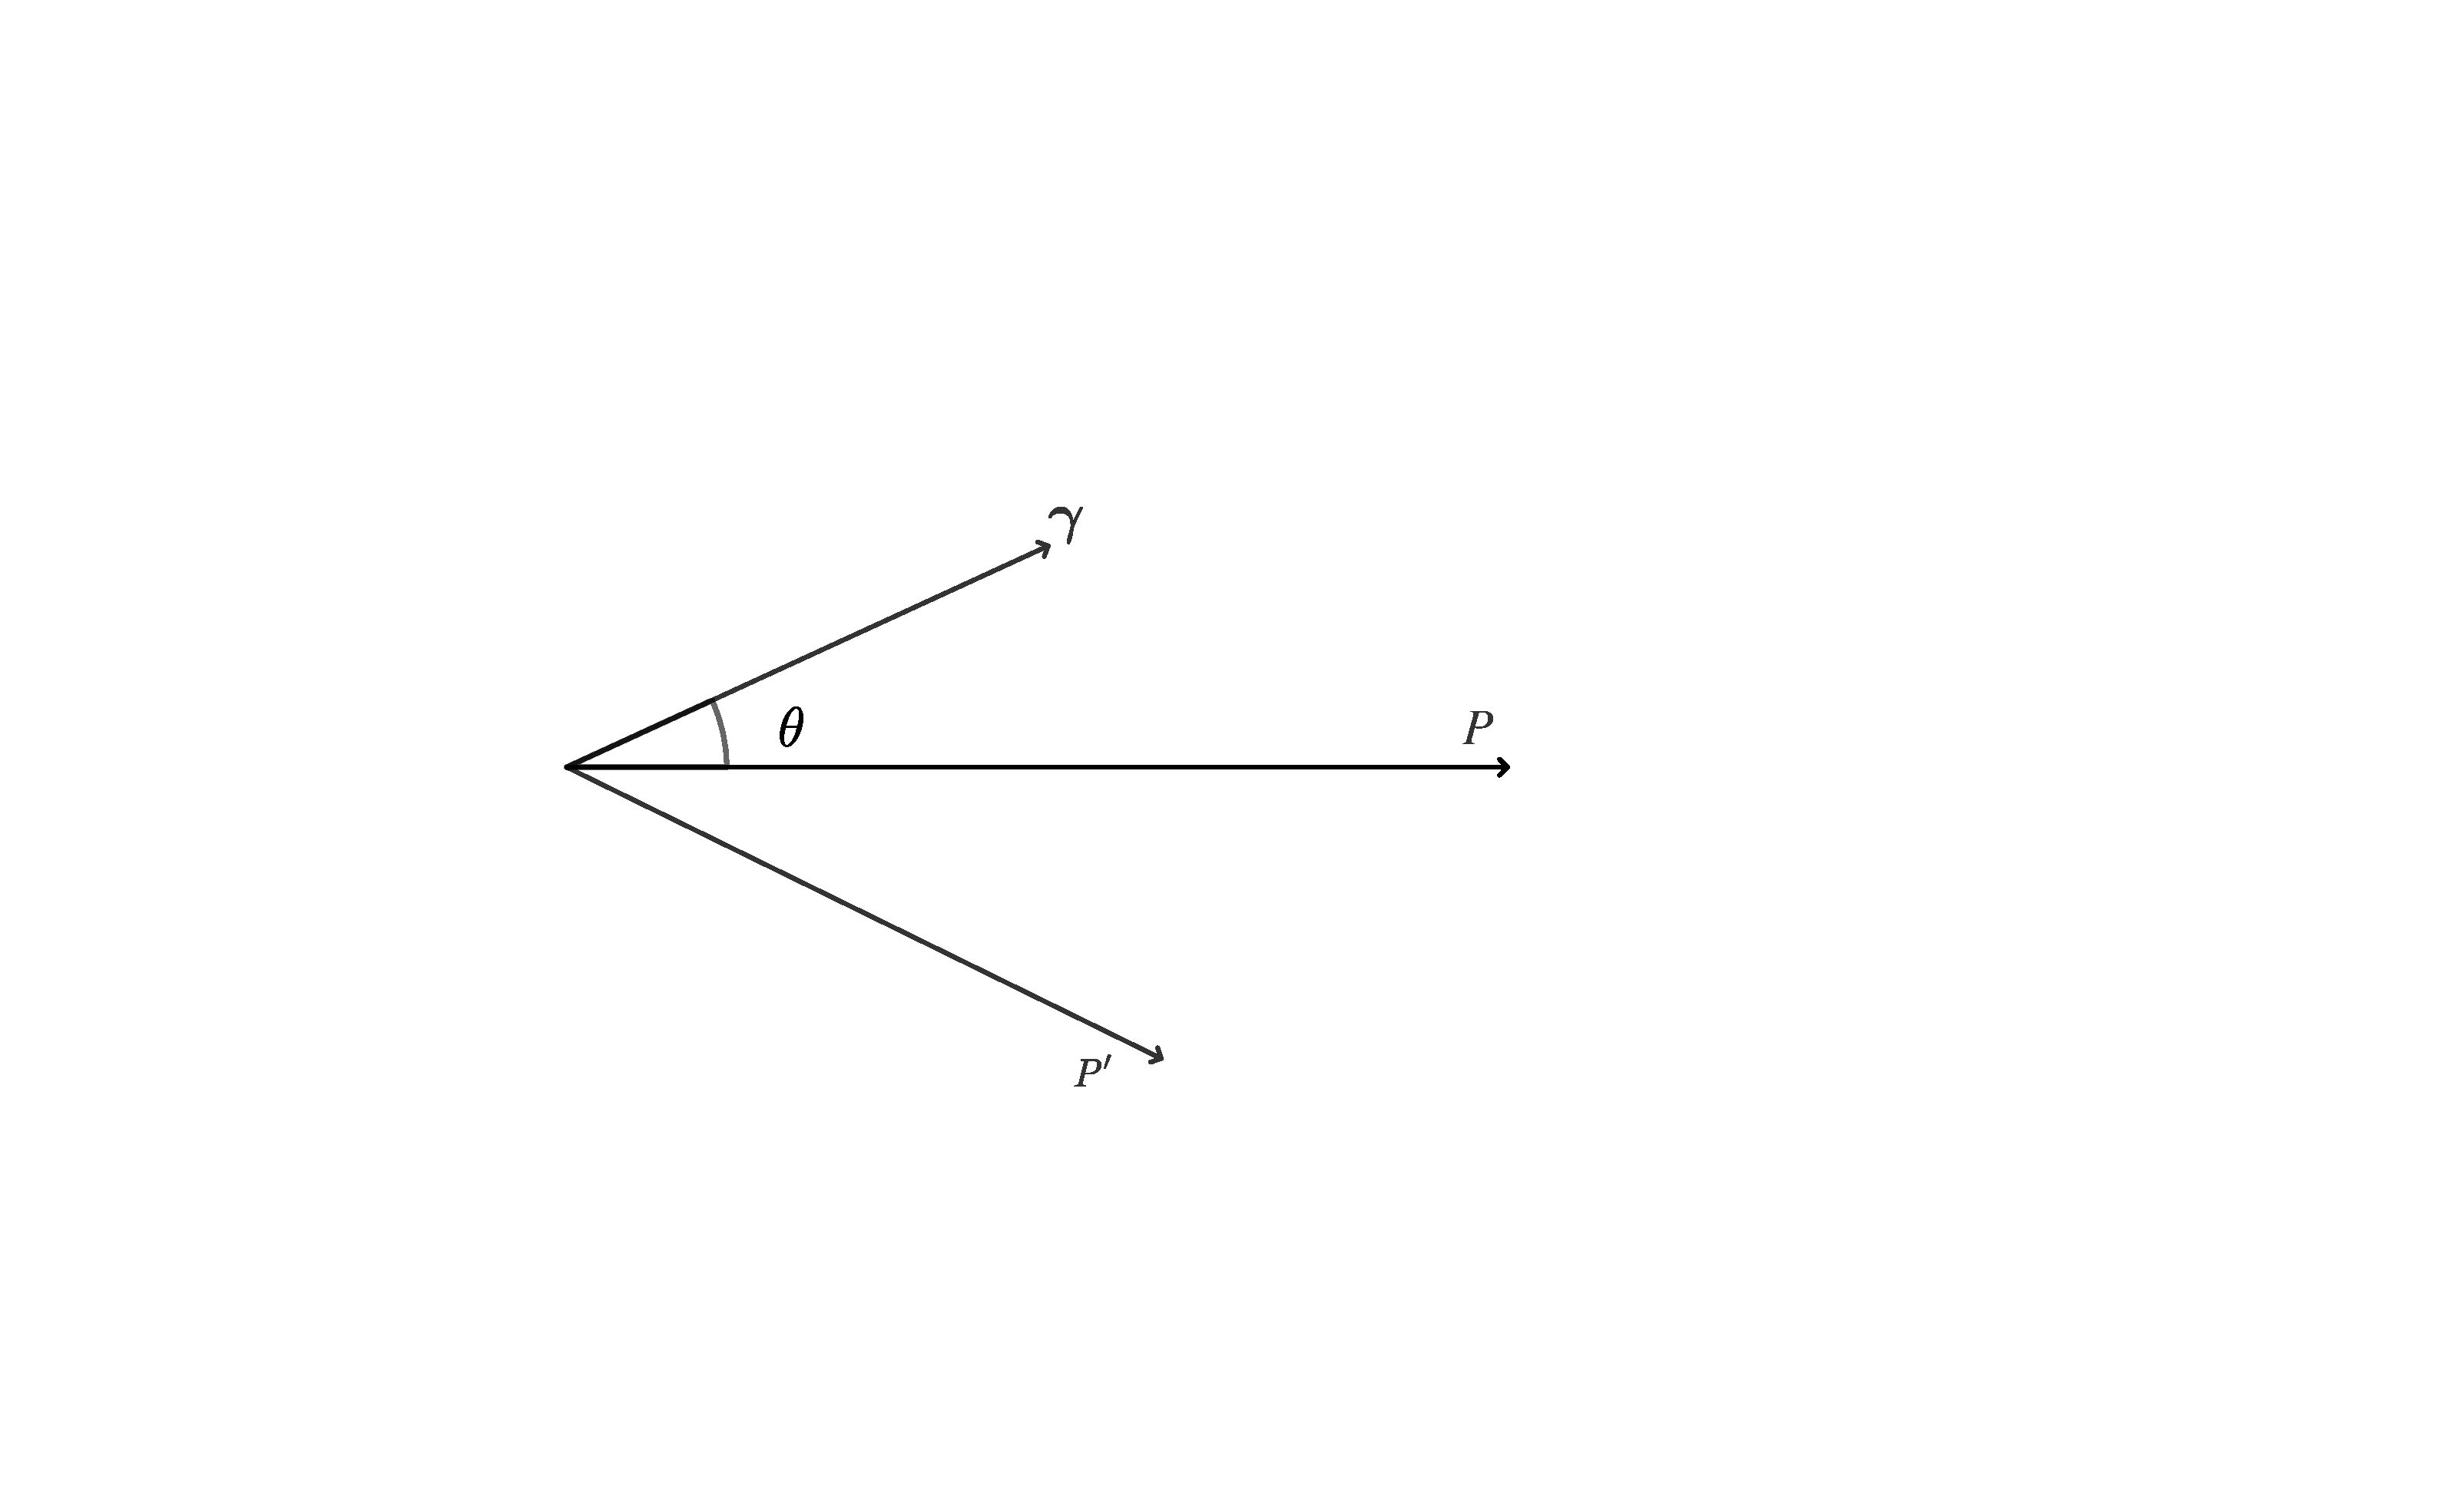
\includegraphics[width=3.5cm,clip]{QM file/figure/1-9}
	\caption{1-4题图}
	\label{fig.1-9}
\end{wrapfigure}
\exercise 高能带电粒子在介质中运动,如其速度$v$超过电磁波在介质中的传播速度,就产生切仑科夫辐射.设介质的折射率为$n$,辐射光与粒子运动方向的夹角为$\theta$.试利用光子的能量,动量公式($E_{\gamma}=\hbar\omega,p_{\gamma}=\hbar k$)以及能量守恒及动量守恒定律,求$\theta$与$n,v$的关系

$\big[\text{提示:光在介质中传播时,}\omega=\dfrac{ck}{n}. \big]$

\exercise 从质量为$m$,半径为$R$的星球表面辐射出频率为$\nu_{0}$的光,当这种光在远离星球处被观测到时,测得的频率$\nu<\nu_{0}$,这种现象称为恒星光谱的“引力红移”.设光子可以当作“质点”,引力质量$m_{\text{光}}=\dfrac{h\nu}{c^{2}}$下,光子离开星球时,必须克服星球对它的万有引力.试根据这种通俗模型导出$\dfrac{\nu}{\nu_{0}}$的公式.

\exercise 来自其他恒星的光掠过太阳(质量$M$,半径$R$)表面时,光线方向发生微小的偏转($\theta$).这个现象曾是广义相对论的实验支柱之一.试利用$1\sim 5$题中光子的“质点”模型对偏转角$\theta$作出量级估算.
\begin{figure}[!h]
	\centering
	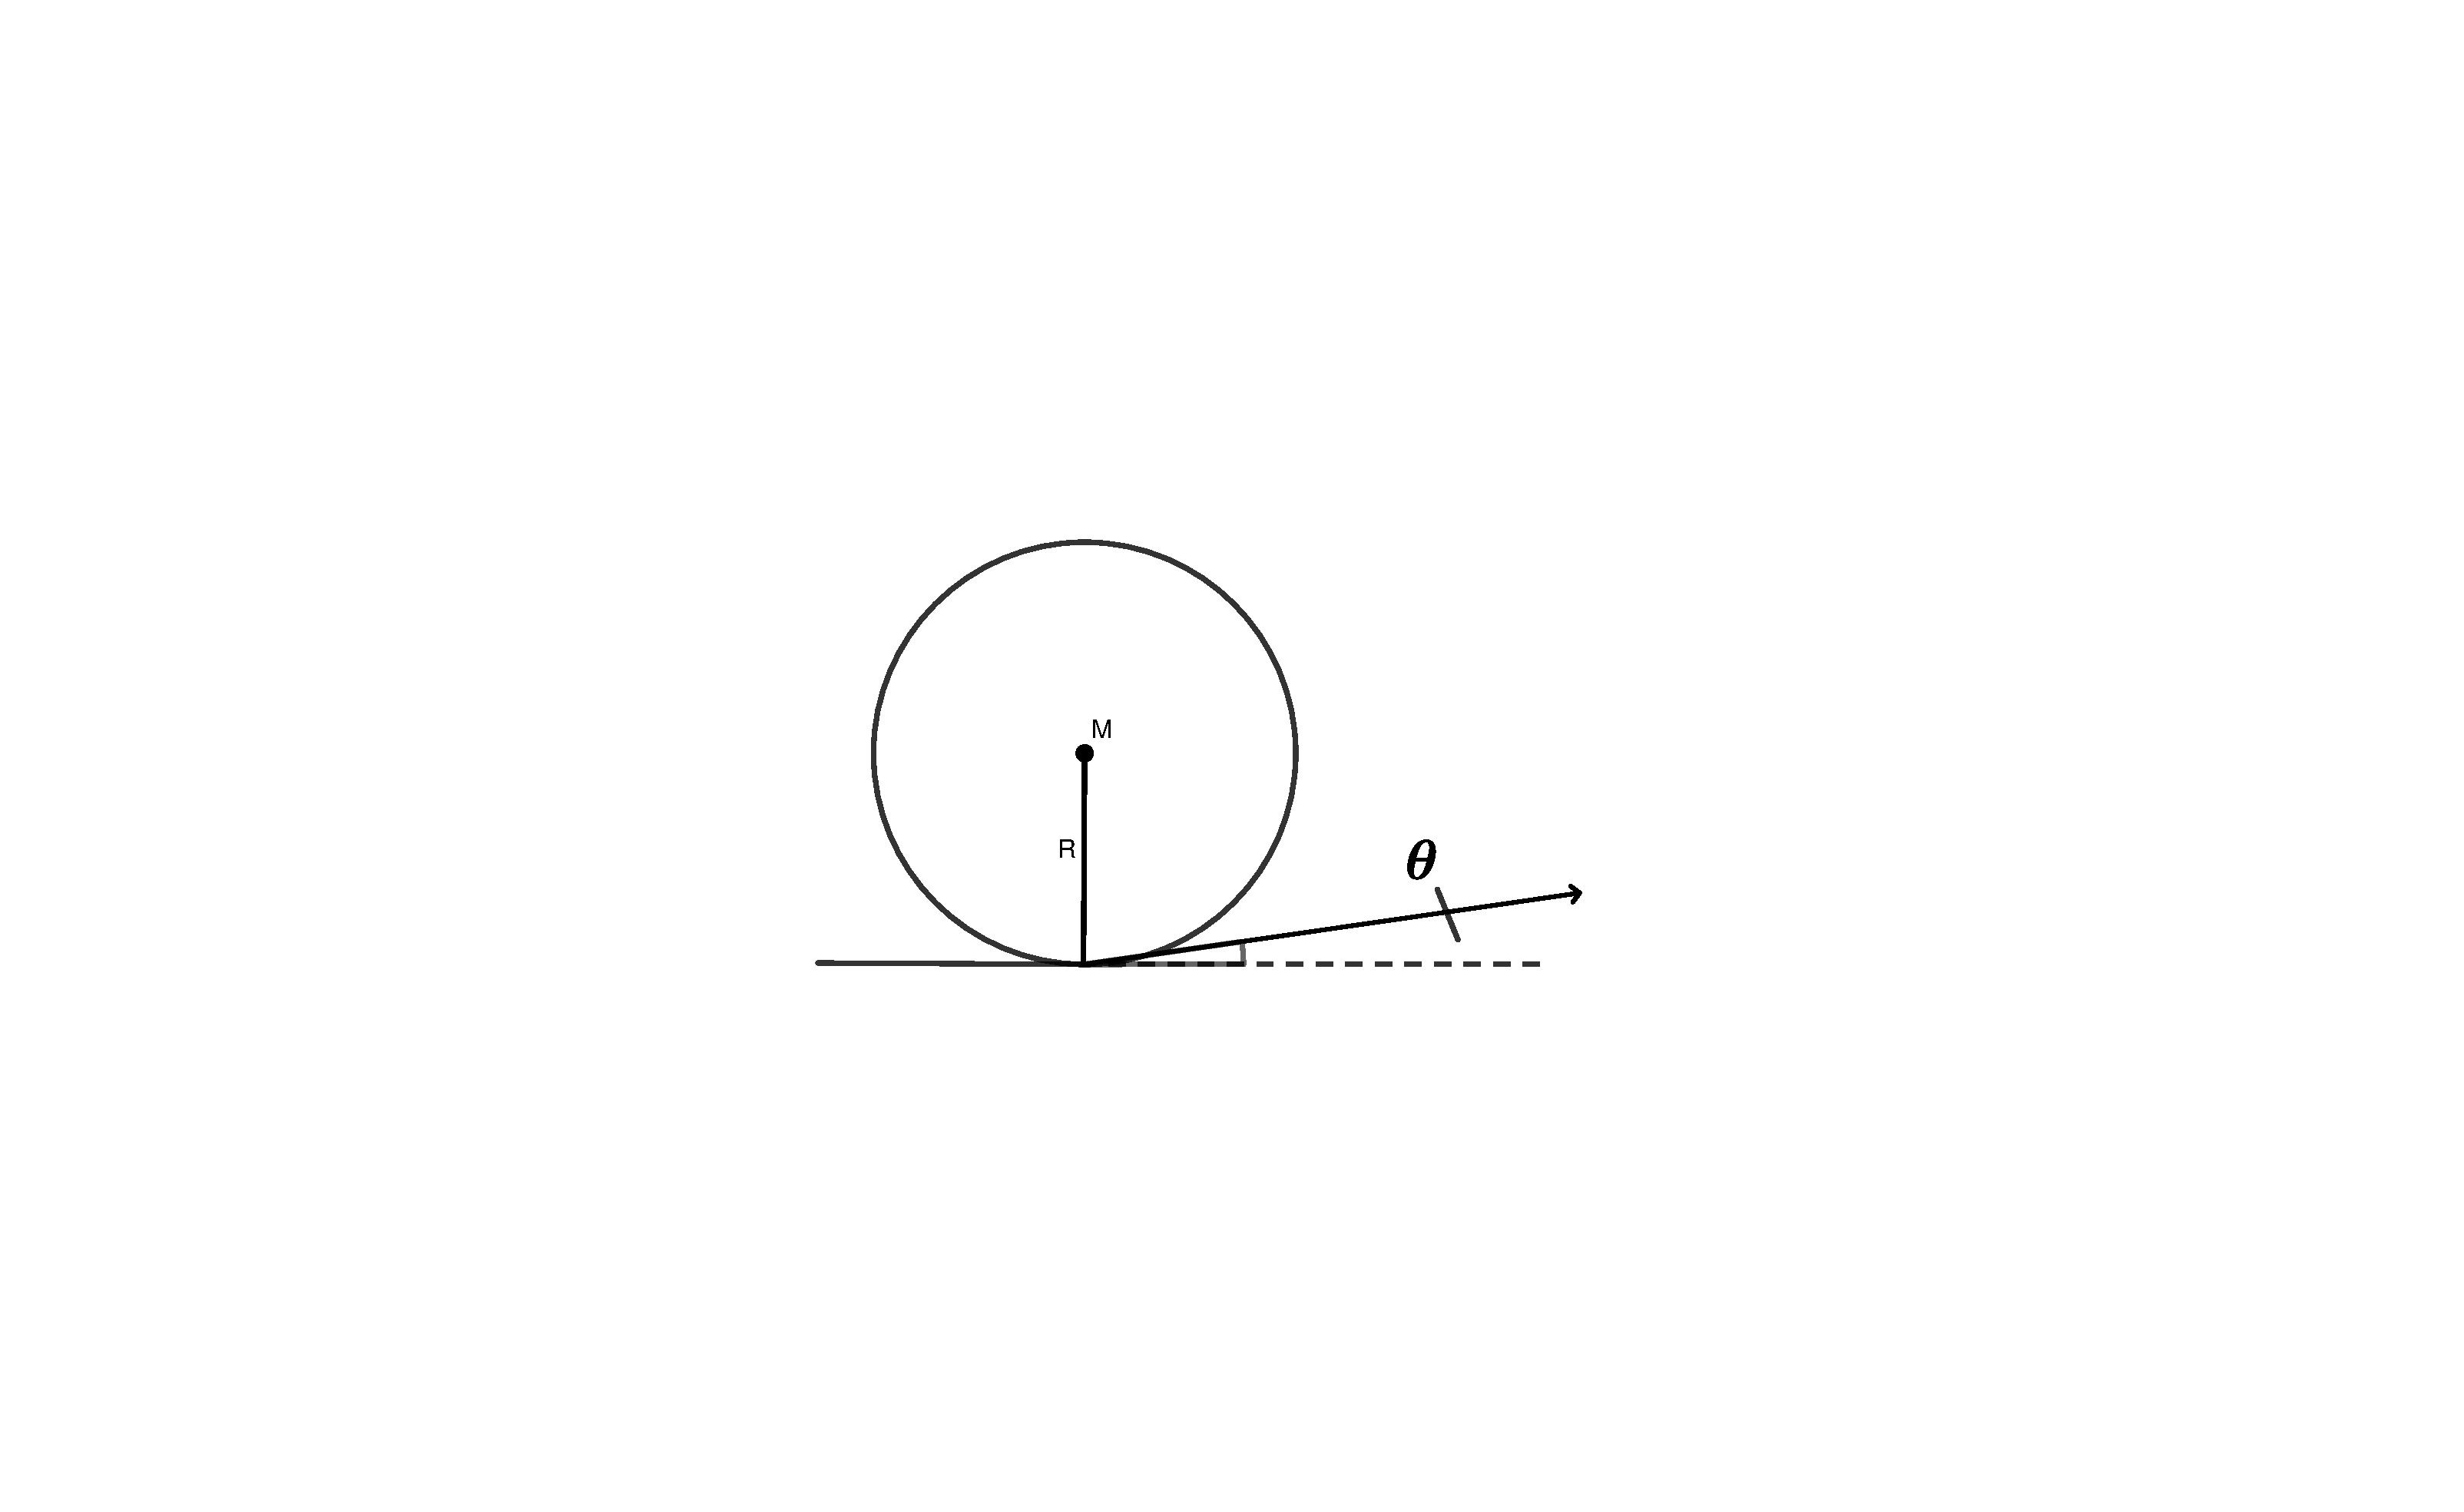
\includegraphics[width=3.5cm,clip]{QM file/figure/1-10}
	\caption{1-6题图}	\label{fig.1-10}
\end{figure}
\exercise 氢原子中电子-质子间库仑吸引力远大于万有引力.求这两种力的比率.理论上,电子与中子间的万有引力也可以使它们形成类似于氢原子的构造,试求这种“引力原子” 的基态半径公式及数值.

\exercise (a) $\mu^{-1}$子电荷为$-e$,质量$m_{\mu}=207m_{e}$,$\mu^{-1}$子与原子核(电荷$Ze$)由于库仑吸引力的作用而形成类似氢原子的构造.称为$\mu$原子.视原子核为点电荷,求$\mu$原子半径公式.
	
\quad (b) 原子核可视为电荷均匀分布的球体, 核半径的经验公式为
\begin{equation*}
	R=r_{0p}Z^{1/3},\quad r_{0p}=1.635\si{fm}
\end{equation*}
对于较大的原子序数$Z$,核半径$R$有可能大于$\mu$原子半径.求出现这种情况的$Z$的临界值$Z_{0}$. 

\exercise 计算原子核(电荷$Ze$,半径$R$)中各质子间库仑排斥能的总和及(按质子)平均值.原子核半径公式见1-8题.当$Z$取多大数值时,每个质子的平均库仑能达到核力结合能(每个核子约8\si{MeV})的量级?

\exercise 电子自旋磁矩等于$\mu_{B}$=$\dfrac{\e\hbar}{2m_{\e}c}$(玻尔磁子).在磁场$(B)$中电子获得的磁作用能大致为$B\mu_{B}$量级.如$B\mu_{B}\sim10^{-3}\si{eV}$,求磁场$B$的量级.

\exercise 估算氢分子转动能级的“解冻温度”.氢分子键长$R=0.74\times10^{-8}\si{cm}$.

\exercise 由于电磁场的真空量子效应,两块相隔距离$d$的不带电大导体平板间产生微弱吸引力设单位面积受力F,试用量纲分析法确定$F$与各基本普适常数及距离$d$的关系.

\exercise { (a) 求室温(T=300 \si{K})下中子的德布罗意波长.
	
	\quad (b) 如上述中子在地面附近垂直下落1\si{m},求波长变化的比率.
}

\exercise 如普朗克常数的值变成现有值的2倍,而其他基本常数之值不变,下列各项数值变为现有值的多少倍?

(a)原子半径 \quad (b)晶体密度 \quad (c)蓄电池的电压

\exercise 质量为$m$的粒子受弹性力$F=-kx(k>0)$作用而作一维简谐振动,按照经典力学可以求出其运动规律为
\begin{equation*}
	x(t)=A\sin(\omega t+\alpha),\quad \omega=\sqrt{\frac{k}{m}}
\end{equation*}
A为振幅谐振子的能量为$E=\dfrac{1}{2}kA^{2}$.以上请读者自行验证.试再利用玻尔-索末菲量子化条件或对应原理证明能量及振幅的量子化结果:
\begin{equation*}
	E_{n}=n\hbar\omega,\quad A_{n}=\sqrt{\frac{2n\hbar}{m\omega}},\quad n=0,1,2,\cdots
\end{equation*}
$\big[$提示:宏观的谐振动电荷,辐射的电磁波频率与振动频率相同.据此,再利用对应原理,很容易得出结论.$\big]$

\exercise 质量为$m$的粒子在大小一定的向心力$\boldsymbol{F}=-\dfrac{k\boldsymbol{r}}{r}$作用下作圆周运动.先用经典力学证明轨道半径$r$,角速度$\omega$,总能量$E$有如下关系:
\begin{equation*}
	r\omega^{2}=\frac{k}{m},\quad \boldsymbol{E}=\frac{3}{2}k\boldsymbol{r}=\frac{3}{2}\frac{k^{2}}{m\omega^{2}}
\end{equation*}
再利用量子化条件或对应原理证明能级的量子化公式:
\begin{equation*}
	E_{n}=\frac{3}{2}\bigg(\frac{\hbar^{2}k^{2}n^{2}}{m} \bigg)^{\frac{1}{3}},\quad n=1,2,3,\cdots
\end{equation*}
 
\end{exercises}



% 第二章 波函数和薛定谔方程
\input{QM file/body/C.two/M02.00-Wave function and Schrödinger's equation}

% 第三章 基本原理
\chapter{基本原理}\label{chp:03} % Fundamentals
% \makebox[5em][s]{} % 短题目拉间距

本章将全面阐述捏子力学的基本原理和基本概念,侧重点将放在力学量的算符表示方面.

% 波函数和算符
\section[波函数和算符]{波函数和算符} \label{sec:03.01} % 
% \makebox[5em][s]{} % 短题目拉间距

本节扼要叙述第二章已经讲过的一些原理和概念,并作适当扩充.

{\heiti 1.状态和波函数}

量子力学的第一个基本概念(基本假设)是,可以用波函数$\varPsi$全面描述微观粒子的运动状态,由$\varPsi$可以得知状态的全部物理性质.$\varPsi$也称态函数.

不考虑粒子的自旋时,$\varPsi$是粒子的坐标(位置)$\boldsymbol{r}$和时间$t$的函数.对于一个随时间变化的运动态,$\varPsi=\varPsi(\boldsymbol{r},t)$;在某个给定的时刻$t_{0}$,$\varPsi=\varPsi(\boldsymbol{r},t_{0})$,是$\boldsymbol{r}$的函数.

波函数的概念是德布罗意物质波思想的发展,是微观粒子具有波动性的数学描述.而波动性的真正含义是概率性,波函数$\varPsi$所描述的状态性质一般都带有概率性的特征,这是迄今人类已经发现并掌握的微观规律的根本特征.波函数的统计诠释
\begin{empheq}{equation}\label{eq31.1}
	\varPsi^{*}\varPsi d\tau\propto \text{粒子在}d\tau\text{中出现概率}
\end{empheq}
给出状态$\varPsi$下粒子空间位置($\boldsymbol{r}$,当作力学量对待)的分布概率.$\S$\ref{sec:03.04}将普遍讨论任何力学量在一定状态下的取值及分布概率.

{\heiti 2.薛定谔方程}

量子力学的另一项基本假设是,运动态的波函数满足薛定谔方程.在简单情况下,如果粒子受到的外界作用可以用势能$V(\boldsymbol{r})$表示,则薛定谔方程为
\begin{empheq}{equation}\label{eq31.2}
	i\hbar\frac{\partial}{\partial t}\varPsi=-\frac{\hbar^{2}}{2m}\nabla^{2}\varPsi+V(\boldsymbol{r})\varPsi
\end{empheq}
薛定谔方程的普遍形式是
\setlength{\mathindent}{12em}
\begin{empheq}{equation}\label{eq31.3}
	i\hbar\frac{\partial}{\partial t}\varPsi=\hat{H}\varPsi
\end{empheq}\eqnormal
其中$\hat{H}$是哈密顿算符.薛定谔方程是微观粒子运动状态随时间变化规律的数学描述,由于它是时间$t$的一阶微分方程,只需给定初始时刻($t_{0}$)的波函数$\varPsi(\boldsymbol{r},t)$.这正是微观领域因果性的表现形式.薛定谔方程保证粒子的空间分布总概率守恒,亦即保证粒子数守恒.

{\heiti 3.定态}

能量具有确定值的运动态称为定态,它的波函数随时间的变化规律具有特别简单的形式:
\setlength{\mathindent}{10em}
\begin{empheq}{equation}\label{eq31.4}
	\varPsi_{E}(\boldsymbol{r},t)=\varPsi_{E}(\boldsymbol{r})e^{-iEt/\hbar}
\end{empheq}
$\varPsi_{E}(\boldsymbol{r})$满足定态薛定谔方程:
\begin{empheq}{equation}\label{eq31.5}
	\hat{H}\varPsi_{E}(\boldsymbol{r})=E\varPsi_{E}(\boldsymbol{r})
\end{empheq}
这是粒子能量的特征方程,它决定粒子运动的能谱.

定态是一种稳定状态,$|\varPsi_{E}(\boldsymbol{r},t)|^{2}$不随时间变化,由它给出的粒子空间分布概率稳定不变.$\S$\ref{sec:03.09}将说明,定态的其他物理性质也都稳定不变.

薛定谔方程\eqref{eq31.2}或\eqref{eq31.3}的通解可以表示成各定态波函数的线性组合,即
\begin{empheq}{equation}\label{eq31.6}
	\varPsi(\boldsymbol{r},t)=\sum_{n}C_{n}\varPsi_{E_{n}}(\boldsymbol{r},t)
\end{empheq}\eqnormal
系数$C_{n}$不随时间改变.

{\heiti 4.力学量和算符}

量子力学的另一项基本概念(基本假设)是,在理论计算中,力学量(实验上可以观测的量)可以用一个算符(算子)来表示,这是经典物理中所没有的新概念,$\S$\ref{sec:02.01}建立薛定谔方程时我们已经初步接触到这个概念.状态用波函数来描述(表示),力学量用算符来表示,可以说是一对孪生的量子力学基本概念(基本假设).

凡是有经典对应的力学量,相应的算符根据下列对应关系而得出:
\begin{empheq}{equation}\label{eq31.7}
	\boldsymbol{r}\rightarrow\boldsymbol{r},\quad\boldsymbol{p}\rightarrow\hat{\boldsymbol{p}}=-i\hbar\nabla
\end{empheq}
因此,纯粹是坐标(位置)的函数的那些经典力学量,其量子力学对应算符仍是坐标的函数,例如势能$V(\boldsymbol{r})$,作用力
\begin{empheq}{equation}\label{eq31.8}
	\boldsymbol{f}(\boldsymbol{r})=-\nabla V(\boldsymbol{r})
\end{empheq}
等等.经典力学中最重要的力学量有位置$\boldsymbol{r}$,动量$\boldsymbol{p}$,速度$\boldsymbol{v}=\frac{\boldsymbol{p}}{m}$,作用力$\boldsymbol{f}$,势能$V(\boldsymbol{r})$,动能$T=\frac{\boldsymbol{p}^{2}}{2m}$,角动量$\boldsymbol{L}=\boldsymbol{r}\times\boldsymbol{p}$,总能(哈密顿量)$H=T+V$,等等.动能的算符表示是
\begin{empheq}{equation}\label{eq31.9}
	\hat{T}=-\frac{\hbar^{2}}{2m}\nabla^{2}=-\frac{\hbar^{2}}{2m}\bigg(\frac{\partial^{2}}{\partial x^{2}}+\frac{\partial^{2}}{\partial y^{2}}+\frac{\partial^{2}}{\partial z^{2}}\bigg)
\end{empheq}
角动量$\boldsymbol{L}$的算符表示是
\begin{empheq}{equation}\label{eq31.10}
	\hat{\boldsymbol{L}}=\boldsymbol{r}\times\hat{\boldsymbol{p}}
	=-i\hbar \boldsymbol{r}\times\nabla
\end{empheq}
即
\begin{empheq}{align*}\label{eq31.10'}
	\hat{L_{x}} &=y\hat{p_{z}}-z\hat{p_{y}}=-\hbar\bigg(y\frac{\partial}{\partial z}-z\frac{\partial}{\partial y}\bigg)	\\
	\hat{L_{y}} &=z\hat{p_{x}}-x\hat{p_{z}}=-\hbar\bigg(z\frac{\partial}{\partial x}-x\frac{\partial}{\partial z}\bigg)	\\
	\hat{L_{z}} &=x\hat{p_{y}}-y\hat{p_{x}}=-\hbar\bigg(x\frac{\partial}{\partial y}-y\frac{\partial}{\partial x}\bigg)
\end{empheq}
$\hat{L}$的模方(俗称“平方”)定义成
\begin{empheq}{equation}\label{eq31.11}
	\hat{\boldsymbol{L}}^{2}=\hat{L_{x}}^{2}+\hat{L_{y}}^{2}+\hat{L_{z}}^{2}
\end{empheq}
角动扯本质上描写粒子运动的旋转性质,因此采用球坐标$(r,\theta,\varphi)$比较方便.$(r,\theta,\varphi)$和$(x,y,z)$的关系是
\begin{empheq}{equation}\label{eq31.12}
	\begin{aligned}
		x &=r\sin\theta\cos\varphi, &y=r\sin\theta\sin\varphi	\\
		z &=r\cos\theta, &x^{2}+y^{2}+z^{2}=r^{2}
	\end{aligned}
\end{empheq}
其他关系见附录\ref{A03}.$\boldsymbol{r}$和$V$的直角坐标和球坐标表示式是
\setlength{\mathindent}{6em}
\begin{empheq}{equation}\label{eq31.13}
	\boldsymbol{r}=\boldsymbol{e_{1}}x+\boldsymbol{e_{2}}y+\boldsymbol{e_{3}}z=\boldsymbol{e_{r}}r
\end{empheq}
\begin{empheq}{equation}\label{eq31.14}
	\begin{split}
		\nabla 
		&=\boldsymbol{e_{1}}\frac{\partial}{\partial x}+\boldsymbol{e_{2}}\frac{\partial}{\partial y}+\boldsymbol{e_{3}}\frac{\partial}{\partial z}	\\
		&=\boldsymbol{e_{r}}\frac{\partial}{\partial r}+\boldsymbol{e_{\theta}}\frac{1}{r}\frac{\partial}{\partial \theta}+\boldsymbol{e}_{\varphi}\frac{1}{r\sin\theta}\frac{\partial}{\partial \varphi}
	\end{split}
\end{empheq}
经过计算(见附录\ref{A03}),得到
\begin{empheq}{equation}\label{eq31.15}
	\begin{aligned}
		\hat{L_{x}} &=-\hbar\bigg(\sin\varphi\frac{\partial}{\partial \theta}+\cot\theta\cos\varphi\frac{\partial}{\partial \varphi}\bigg)	\\
		\hat{L_{y}} &=-\hbar\bigg(-\cos\varphi\frac{\partial}{\partial \theta}+\cot\theta\sin\varphi\frac{\partial}{\partial \varphi}\bigg)	\\
		\hat{L_{z}} &=-\hbar\bigg(\frac{\partial}{\partial \varphi}\bigg)
	\end{aligned}
\end{empheq}
\begin{empheq}{equation}\label{eq31.16}
	\hat{\boldsymbol{L}}^{2}=-\hbar^{2}\bigg[\frac{1}{\sin\theta}\frac{\partial}{\partial \theta}\sin\theta\frac{\partial}{\partial \theta}+\frac{1}{\sin^{2}\theta}\frac{\partial^{2}}{\partial \varphi^{2}}\bigg]
\end{empheq}\eqnormal

{\heiti 5.力学量算符的本征方程}

第二章中讨论过几种定态问题,能级(能量本征值)和定态波函数一起由定态薛定谔方程
\setlength{\mathindent}{12em}
\begin{empheq}{equation*}
	\hat{H}\varPsi_{E}=E\varPsi_{E}
\end{empheq}
解出.\eqref{eq31.5}式也称为算符$\hat{H}$的本(特)征方程,$E$称为本(特)征值,$\varPsi_{E}$称为本(特)征函数.本征值$E$就是能量的可能取值,$\varPsi_{E}$则是能量取确定值$E$的状态的波函数.这个概念可以推广到任何力学量.设有力学量$A$,其算符表示为$\hat{A}$,设参数(常数)$a$及波函数$\varPsi_{n}(r)$满足方程:
\begin{empheq}{equation}\label{eq31.17}
	A\varPsi_{n}=a\varPsi_{n}
\end{empheq}\eqnormal
则称$a$为力学量算符$\hat{A}$的本征值,$\varPsi_{n}$为$\hat{A}$的本征函数.上式称为算符$\hat{A}$的本征方程.作为一项基本假定,凡是满足本征方程\eqref{eq31.17}的任何一个$a$值可以认为就是力学量$A$的一个可能取值,而$\varPsi_{n}$则是$A$取确定值$a$时状态的波函数.如果只有某些特殊的$a$值(以及相应的$\varPsi_{n}$)才能满足本征方程\eqref{eq31.17},力学量$A$的取值就是量子化的.简言之,由力学量算符的本征方程解出的全部本征值,就是相应力学量的可能取值.如用测量仪器测最这个力学量的取值,只能浏得其本征值.这个观点是量子力学的一项基本假设.

\example 求$\hat{L}^{z}$的本征值和本征函数.

\solution 考虑到$L_{z}$和$\hbar$量纲相同,以$m\hbar$表示$\hat{L}^{z}$的本征值,$m$为无量纲纯数,待定.本征方程为
\begin{empheq}{equation}\label{eq31.18}
	\hat{L}_{z}\varPsi=-i\hbar\frac{\partial}{\partial \varphi}\varPsi=n\hbar\varPsi
\end{empheq}
用分离变量法,令
\setlength{\mathindent}{11em}
\begin{empheq}{equation}\label{eq31.19}
	\varPsi=u(r,\theta)\Phi(\varphi)
\end{empheq}
代入\eqref{eq31.7}式,显然$u(r,\theta)$可以是任意函数,$\Phi(\varphi)$则满足方程:
\begin{empheq}{equation*}
	\frac{d}{d\varphi}\Phi=im\Phi
\end{empheq}
解出
\begin{empheq}{equation}\label{eq31.20}
	\Phi=Ce^{im\varphi}
\end{empheq}
C为归一化常数.变量$\varphi$是多值的,由空间某一点开始,按右手螺旋方向绕$z$轴一周,回到出发点,$\varphi$值增加$2\pi$.而波函数$\varPsi$作为状态全部物理性质的数学描述,应该是$\boldsymbol{r}$的单值函数,因此$\Phi(\varphi)$应该满足单值条件\footnote[1]{关于单值条件的更严密的论证可以从$\hat{L}_{z}$的厄密性出发,请读者读完$\S$\ref{sec:03.05}后自行证明.}:
\begin{empheq}{equation}\label{eq31.21}
	\Phi(\varphi+2\pi)=\Phi(\varphi)
\end{empheq}
为了满足单值条件,\eqref{eq31.20}式中必须取
\begin{empheq}{equation}\label{eq31.22}
	m=0,\pm1,\pm2,\cdots
\end{empheq}
因此
\begin{empheq}{equation*}
	L_{z}=m\hbar=0,\pm\hbar,\pm2\hbar,\cdots
\end{empheq}
这结果和玻尔量子论一致,并且已经被实验测量所证实.

如略去\eqref{eq31.18}式中任意函数$u(r,\theta)$,并相应地规定归一化条件为
\begin{empheq}{equation}\label{eq31.23}
	\int_{0}^{2\pi}\Phi^{*}\Phi d\varphi=1
\end{empheq}\eqnormal
容易求出\eqref{eq31.9}式中归一化系数(取为正实数)$C=\frac{1}{\sqrt{2\pi}}$,所以$\hat{L}_{z}$的本征函数为
\setlength{\mathindent}{6em}
\begin{empheq}{equation}\label{eq31.24}
	\boxed{\Phi_{m}(\varphi)=\frac{1}{\sqrt{2\pi}}e^{im\varphi},\quad m=0,\pm1,\pm2,\cdots}
\end{empheq}\eqnormal
\pskip

% 态叠加原理
\section[态叠加原理]{态叠加原理} \label{sec:03.02} % 
% \makebox[5em][s]{} % 短题目拉间距

不同波动状态之间,常有一定联系.例如光栅衍射,衍射光束可以用分光镜分解成各种单色平面光.因此,有理由认为,即使是在分解前,该光束也是由各种单色平面光波叠加而成,表现在波函数上,就是
\setlength{\mathindent}{6em}
\begin{empheq}{equation}\label{eq32.1}
	\varPsi(\boldsymbol{r},t)=\sum_{n}C_{n}\varPsi_{n}(\boldsymbol{r},t)=\sum_{n}C_{n}e^{i\boldsymbol{k}_{n}\cdot\boldsymbol{r}-\omega_{n}t}
\end{empheq}\eqnormal
这里$\varPsi$表示$\boldsymbol{k}=\boldsymbol{k}_{n}$,$\omega=\omega_{n}$的单色平面光波波函数.

波函数之间的这种线件叠加关系,在量子力学中具有根本意义.作为一项基本假设,量子力学认为:

(1) 物理体系的任何一种状态(波函数$\varPsi$)总可以认为是由某些其他状态(波函数$\varPsi_{1},\varPsi_{2},\cdots$)线性叠加而成,即
\begin{empheq}{equation}\label{eq32.2}
	\varPsi=C_{1}\varPsi_{1}+C_{2}\varPsi_{2}+\cdots
\end{empheq}
$C_{1},C_{2},\cdots$为常数(可以是复数).

(2) 如果$\varPsi_{1},\varPsi_{2},\cdots$是可以实现的状态(波函数),则它们的任何线性叠加式\eqref{eq32.2}总是表示一种可以实现的状态(波函数).

(3) 当物理体系处于叠加态\eqref{eq32.2}式,可以认为该体系部分地处于$\varPsi_{1}$态,部分地处于$\varPsi_{2}$态,等等.

以上各点,常被称为“态叠加原理”.

从实际应用来说,最重要的一种情况是,$\varPsi_{1},\varPsi_{2},\cdots$是某个力学量算符$\hat{A}$的本征函数,这时叠加式\eqref{eq32.2}具有特别重要的物理意义,将在$\S$\ref{sec:03.04}阐述.

注意以上所说的叠加都是指\eqref{eq32.2}式那样的线性叠加.至于波函数之间的非线性关系,例如:
\begin{empheq}{equation*}
	\varPsi=\varPsi_{1}+|\varPsi_{2}|+(\varPsi_{3})^{2}+\sqrt{\varPsi_{4}}+\cdots
\end{empheq}
即使这种关系在数学上确实存在,也不认为它有任何物理意义.

在整个量子力学理论中,态叠加原理起着统制全局的作用,为了和它协调,量子力学的基本方程——薛定谔方程就是一个线性方程,表示力学量的算符都是线性算符,等等.量子力学理论为什么要以态叠加原理作为基础,采取线性结构,并没有什么先验的理由,但是半个多世纪以来量子力学在各方面获得的巨大成功表明这样做是正确的.也有人进行着建立非线性量子力学的工作,但还远远没有获得成功.

必须指出,量子力学中态叠加的含义和经典物理中波的叠加含义是不同的.例如一个态自身和自身叠加:
\setlength{\mathindent}{11em}
\begin{empheq}{equation*}
	\varPsi_{1}+\varPsi_{1}=2\varPsi_{1}=\varPsi
\end{empheq}\eqnormal
根据波函数的统计诠释,必须认为$\varPsi=2\varPsi_{1}$也$\varPsi_{1}$也代表同一种状态.而对于经典波动,$2\varPsi_{1}$的振幅为$\varPsi_{1}$的2倍,二者具有不同的物理性质,例如前者的能量是后者的4倍,因此代表两种不同的波动状态.

% 线性算符
\section[线性算符]{线性算符} \label{sec:03.03} % 
% \makebox[5em][s]{} % 短题目拉间距

线性算符(子)是量子力学的基本数学工具,本节对此作初浅介绍,叙述力求简明,不追求论证的严格性, 以利初学者阅读.

量子力学中,可以作用于波函数并且符合下列运算法则的算符$\hat{A}$称为线性算符,
\begin{empheq}{equation}\label{eq33.1}
	\hat{A}(C_{1}\varPsi_{1}+C_{2}\varPsi_{2})=C_{1}\hat{A}\varPsi_{1}+C_{2}\hat{A}\varPsi_{2}
\end{empheq}
其中$\varPsi_{1},\varPsi_{2}$是任意波函数(表示可以实现的状态),$C_{1},C_{2}$是常数(复数).

$\S$\ref{sec:03.01}所列举的力学量算符显然都是线性算符.\eqref{eq33.1}式表明,线性算符作用于几个波函数的叠加式时,可以逐项分别作用,而对常系数则不起作用.

诸如开方,取绝对值,取复共轭等运算,则为非线性运算,如果定义出相应的算符,就是非线性算符.例如定义平方根算符$\sqrt{\quad}$,作用规则为
\begin{empheq}{equation*}
	\sqrt{\quad}\varPsi=\sqrt{\varPsi}=(\varPsi)^{\frac{1}{2}}
\end{empheq}
则
\begin{empheq}{equation*}
	\sqrt{\quad}C\varPsi=\sqrt{C\varPsi}=\sqrt{C}\sqrt{\varPsi}
\end{empheq}
常系数$C$也受到作用(被开方),所以$\sqrt{\quad}$算符为非线性算符.

以后凡是提到“算符”,均指线性算符.

算符$\hat{A},\hat{B}$之和(差)按下式定义,
\begin{empheq}{equation}\label{eq33.2}
	(\hat{A}\pm\hat{B})\varPsi=\hat{A}\varPsi\pm\hat{B}\varPsi
\end{empheq}
其中$\varPsi$是任意波函数.上式中$\hat{A}\varPsi$和$\hat{B}\varPsi$的性质都是波函数,次序可以颠倒,因此
\begin{empheq}{equation*}
	(\hat{A}+\hat{B})\varPsi=\hat{A}\varPsi+\hat{B}\varPsi=\hat{B}\varPsi+\hat{A}\varPsi=(\hat{B}+\hat{A})\varPsi
\end{empheq}
亦即
\begin{empheq}{equation}\label{eq33.3}
	\hat{A}+\hat{B}=\hat{B}+\hat{A}\quad\text{(加法交换律)}
\end{empheq}

算符$\hat{A},\hat{B}$之积仍为算符,按下式定义,
\begin{empheq}{equation}\label{eq33.4}
	(\hat{A}\hat{B})\varPsi=\hat{A}(\hat{B}\varPsi)
\end{empheq}
其中$\varPsi$为任意波函数(下同).例如
\begin{empheq}{align*}
	(\hat{p}_{x\hat{p}y})\varPsi &=\hat{p}_{x}(\hat{p}_{y}\varPsi)
	=-i\hbar\frac{\partial}{\partial x}\bigg(-i\hbar\frac{\partial}{\partial y}\varPsi\bigg)	\\
	&=-\hbar^{2}\frac{\partial^{2}}{\partial x\partial y}\varPsi
\end{empheq}
所以
\begin{empheq}{equation*}
	\hat{p}_{x}\hat{p}_{y}=-\hbar^{2}\frac{\partial^{2}}{\partial x\partial y}
\end{empheq}
显然
\begin{empheq}{equation}\label{eq33.5}
	\hat{p}_{x}\hat{p}_{y}=\hat{p}_{y}\hat{p}_{x}
\end{empheq}
又如
\begin{empheq}{align*}
	(\hat{p}_{x}\hat{x})\varPsi &=\hat{p}_{x}(\hat{x}\varPsi)
	=-i\hbar\frac{\partial}{\partial x}(x\varPsi)	\\
	&=-i\hbar\bigg(x\frac{\partial}{\partial x}\varPsi+\varPsi\bigg)
	=(\hat{x}\hat{p}_{x}-i\hbar)\varPsi
\end{empheq}
所以算符$\hat{x}\hat{p_{x}}$与$\hat{p_{x}}\hat{x}$不相等,它们的关系是
\begin{empheq}{equation}\label{eq33.6}
	\hat{x}\hat{p_{x}}-\hat{p_{x}}\hat{x}=i\hbar
\end{empheq}
这里将$i\hbar$(常数)也作为算符对待.

\eqref{eq33.5}式和\eqref{eq33.6}式代表了两种典型的算符关系,即对易和不对易.一般说,如$\hat{A}\hat{B}=\hat{B}\hat{A}$,则称$\hat{A}$与$\hat{B}$可对易,或简称$\hat{A},\hat{B}$对易;如$\hat{A}\hat{B}\neq\hat{B}\hat{A}$,则称$\hat{A}$与$\hat{B}$不(可)对易.\eqref{eq33.5}式表明,动量算符的各个分量是相互对易的.\eqref{eq33.6}式表明,$\hat{p}$与$x$(作为算符)是不对易的容易发现,动量算符和位置算符的不同分量是对易的,如
\begin{empheq}{equation}\label{eq33.7}
	\hat{x}\hat{p}_{y}=\hat{p}_{y}\hat{x},\quad \hat{y}\hat{p}_{x}=\hat{p}_{x}\hat{y}
\end{empheq}
等等.力学扯算符之间的不可对易性,是量子力学特有的概念,经典物理中没有类似的概念.

算符$\hat{A}$的$n$(正整数)次幕定义成$n$个$\hat{A}$连乘,如
\begin{empheq}{equation}\label{eq33.8}
	\hat{A}^{2}=\hat{A}\hat{A},\quad \hat{A}^{3}=\hat{A}\hat{A}\hat{A}
\end{empheq}
如再定义
\begin{empheq}{equation}\label{eq33.9}
	\hat{A}^{0}=1
\end{empheq}
显然就有
\begin{empheq}{equation}\label{eq33.10}
	\hat{A}^{n}\hat{A}^{m}=\hat{A}^{m}\hat{A}^{n}=\hat{A}^{n+m}
\end{empheq}
$n,m$为非负整数.

如存在算符$\hat{B}$,使$\hat{B}\hat{A}=\hat{A}\hat{B}=1$,则可以定义$\hat{B}=\hat{A}^{-1}$,称为$\hat{A}$的逆算符.什么样的算符存在逆算符?这问题说来话长,暂不讨论.

波函数$\varPsi$的复共轭记为$\varPsi^{*}$,即
\begin{empheq}{equation*}
	\varPsi=u+iv,\quad \varPsi^{*}=u-iv\quad\text{(}u,n\text{为实数)}
\end{empheq}

对于各种可能的状态(波函数)$\varPsi_{1},\varPsi_{2},\cdots,\varPsi_{i},\cdots$,定义算符$\hat{A}$的“矩阵元”
\begin{empheq}{equation}\label{eq33.11}
	A_{ij}=\int_{\text{全}}\varPsi_{i}^{*}\hat{A}\varPsi_{j}d\tau
\end{empheq}
显然,定义一个算符$\hat{A}$,相当于规定了全体$A_{ij}$之值.注意$A_{ij}$一般是复数.

以下引入共轭算符的概念.$\hat{A}$的共枙记为$\hat{A}^{+}$,定义如下:对于任意波函数$\varPsi_{1},\varPsi_{2},\cdots,\varPsi_{i},\cdots$,定义$\hat{A}^{+}$的“矩阵元”为
\setlength{\mathindent}{5em}
\begin{empheq}{equation}\label{eq33.12}
	A_{ij}^{+}=\int_{\text{全}}\varPsi_{i}^{*}\hat{A}^{*}\varPsi_{j}d\tau=(A_{ij})^{*}
	=\int_{\text{全}}\varPsi_{j}(\hat{A}\varPsi_{i})^{*}d\tau
\end{empheq}
这种定义形式上很抽象,但是对于一般的常用算符,利用\eqref{eq33.12}式很容易找出其共轭算符.例如:

(1) $\hat{A}=\lambda$(常数),由\eqref{eq33.12}式易见$\hat{A}^{+}=\lambda^{*}$.

(2) $\hat{A}=\frac{\partial}{\partial x}$(以一维问题为例),由\eqref{eq33.12}式可得
\begin{empheq}{align*}
	\int_{-\infty}^{\infty}\varPsi_{i}^{*}\bigg(\frac{\partial}{\partial x}\bigg)^{*}\varPsi_{j}dx
	&=\int_{-\infty}^{\infty}\varPsi_{j}\bigg(\frac{\partial}{\partial x}\varPsi_{i}\bigg)^{*}dx	\\
	&=\varPsi_{j}\varPsi_{i}^{*}\bigg|_{-\infty}^{\infty}-\int_{-\infty}^{\infty}\varPsi_{i}^{*}\frac{\partial}{\partial x}\varPsi_{j}dx	\\
	&=\int_{-\infty}^{\infty}\varPsi_{i}^{*}\bigg(-\frac{\partial}{\partial x}\bigg)\varPsi_{j}dx
\end{empheq}\eqnormal
(由于$\varPsi_{i},\varPsi_{j}$描述真实状态,$x\rightarrow\pm\infty$处$\varPsi_{i}$,$\varPsi_{j}\rightarrow 0$)比较上式两端,即得
\begin{empheq}{equation}\label{eq33.13}
	\bigg(\frac{\partial}{\partial x}\bigg)^{*}=-\frac{\partial}{\partial x}
\end{empheq}
同样应有
\begin{empheq}{equation*}\label{eq33.13'}
	\bigg(\frac{\partial}{\partial y}\bigg)^{*}=-\frac{\partial}{\partial y},\quad \bigg(\frac{\partial}{\partial z}\bigg)^{*}=-\frac{\partial}{\partial z}
	\tag{$3.3.13^{\prime}$}
\end{empheq}
因此
\begin{empheq}{equation}\label{eq33.14}
	\nabla^{*}=-\nabla
\end{empheq}

利用定义式\eqref{eq33.12},容易证明:
\begin{empheq}{equation}\label{eq33.15}
	(\hat{A}^{+})^{+}=\hat{A}
\end{empheq}

对于任意两个线性算符$\hat{A},\hat{B}$,容易证明:
\begin{empheq}{equation}\label{eq33.16}
	(\hat{A}\pm\hat{B})^{+}=\hat{A}^{+}\pm\hat{B}^{+}
\end{empheq}
\begin{empheq}{equation}\label{eq33.17}
	(\hat{A}\hat{B})^{+}=\hat{B}^{+}\hat{A}^{+}
\end{empheq}
\eqref{eq33.17}式证明如下:反复利用\eqref{eq33.12}式,可得
\setlength{\mathindent}{5em}
\begin{empheq}{align*}
	 &\int\varPsi_{i}^{*}(\hat{A}\hat{B})^{*}\varPsi_{j}d\tau
	=\bigg[\int\varPsi_{j}^{*}\hat{A}(\hat{B}\varPsi_{i})d\tau\bigg]^{*}
	=\int(\hat{B}\varPsi_{i})^{*}\hat{A}^{+}\varPsi_{j}d\tau	\\
	=&\int(\hat{A}^{+}\varPsi_{j})(\hat{B}\varPsi_{i})^{*}d\tau
	=\int\varPsi_{i}^{*}\hat{B}^{+}(\hat{A}^{+}\varPsi_{j})d\tau	\\
	=&\int\varPsi_{i}^{*}(\hat{B}^{+}\hat{A}^{+})\varPsi_{j}d\tau
\end{empheq}\eqnormal
比较两端,即得\eqref{eq33.17}式.上式中所有积分均为全空间积分.

如果$\hat{A}^{+}=\hat{A}$,则称$\hat{A}$为厄密算符或自共轭算符.利用\eqref{eq33.13}至\eqref{eq33.17}式,容易验明$\S$\ref{sec:03.01}中提到的$\boldsymbol{r},\boldsymbol{p},T,V,H,\boldsymbol{L}$等力学量算符都是厄密算符.

注意,如$\hat{A},\hat{B}$均为厄密算符,即$\hat{A}^{+}=\hat{A},\hat{B}^{+}=\hat{B}$,则($\hat{A}+\hat{B}$)是厄密算符,而$\hat{A}\hat{B}$是否为厄密算符取决于$\hat{A},\hat{B}$是否对易.如$\hat{A}\hat{B}=\hat{B}\hat{A}$,则$\hat{A}\hat{B}$是厄密算符;如$\hat{A}\hat{B}\neq\hat{B}\hat{A}$,则$\hat{A}\hat{B}$就不是厄密算符.

关于厄密算符的本征值和本征函数,可以证明下述定理:

定理(1)$\quad$厄密算符的本征值为实数.

证明:设$\hat{A}^{+}=\hat{A}$,以$a$和$\varPsi_{a}$表示$\hat{A}$的一个本征值和相应的本征函数,满足本征方程:
\begin{empheq}{equation}\label{eq33.18}
	\hat{A}\varPsi_{n}=a\varPsi_{a}
\end{empheq}
以$\varPsi_{n}^{*}$左乘上式,并对全空间积分,得到
\setlength{\mathindent}{5em}
\begin{align*}
	a\int\varPsi_{n}^{*}\varPsi_{n}d\tau
	&=\int\varPsi_{a}^{*}\hat{A}\varPsi_{a}d\tau=\in\varPsi_{a}^{*}\hat{A}^{*}\varPsi_{n}d\tau
	\intertext{利用\eqref{eq33.13}式,}
	&=\bigg(\int\varPsi_{a}^{*}\hat{A}\varPsi_{a}d\tau\bigg)^{*}=a^{*}\int\varPsi_{a}^{*}\varPsi_{a}d\tau
\end{align*}\eqnormal
比较两端,即得$a=a^{*}$,即$a$为实数.

两个波函数$\varPsi_{1},\varPsi_{2}$如果满足关系:
\begin{empheq}{equation}\label{eq33.19}
	\int_{\text{全}}=\varPsi_{1}^{*}\varPsi_{2}d\tau=0
\end{empheq}
则称$\varPsi_{1},\varPsi_{2}$“正交”.

定理(2)$\quad$厄密算符的任何两个对应于不同本征值的本征函数互相正交.

证明:设$\hat{A}=\hat{A}^{+}$,以$a_{1},a_{2}$表示两个本征值,$\varPsi_{1},\varPsi_{2}$为相应的本征函数,满足本征方程:
\begin{empheq}{equation*}
	\hat{A}\varPsi_{1}=a_{1}\varPsi_{1}
\end{empheq}
\begin{empheq}{equation*}
	\hat{A}\varPsi_{2}=a_{2}\varPsi_{2}
\end{empheq}
以$\varPsi_{1}^{*}$左乘第一式,对全空间积分,得到
\begin{empheq}{equation}\label{eq33.20}
	a_{1}\int\varPsi_{2}^{*}\varPsi_{1}d\tau=\int\varPsi_{2}^{*}\hat{A}\varPsi_{1}d\tau
\end{empheq}
以$\varPsi_{1}^{*}$左乘第二式,也对全空间积分,得到
\begin{empheq}{equation*}
	a_{2}\int\varPsi_{1}^{*}\varPsi_{2}d\tau=\int\varPsi_{1}^{*}\hat{A}\varPsi_{2}d\tau
\end{empheq}
取复共轭,并利用\eqref{eq33.13}式,即得
\setlength{\mathindent}{6em}
\begin{empheq}{equation}\label{eq33.20'}
	a_{2}\int\varPsi_{2}^{*}\varPsi_{1}d\tau
	=\bigg(\int\varPsi_{1}^{*}\hat{A}\varPsi_{1}d\tau\bigg)^{*}
	=\int\varPsi_{2}^{*}\hat{A}\varPsi_{1}d\tau
	\tag{$3.3.20^{\prime}$}
\end{empheq}\eqnormal
\eqref{eq33.20}和\eqref{eq33.20'}式右端相等,由于已设$a_{1}\neq a_{2}$,所以
\begin{empheq}{equation*}
	\int_{\text{全}}\varPsi_{2}^{*}\varPsi_{1}d\tau=0
\end{empheq}
即$\varPsi_{1},\varPsi_{2}$正交.

有时,厄密算符($\hat{A}$)的某个本征值($a_{n}$)对应的独立本征函数不止一个.设与本征值$a_{n}$对应的本征函数为$\varPsi_{n1},\varPsi_{n2},\cdots,\varPsi_{nf}$,($f$称为本征值$a_{n}$的简并度)它们互相线性独立,但是可能不正交,可以证明(略),将这$f$个简并态线性叠加,总能重新组成$f$个互相独立而且互相正交的新态,它们仍然是相应于本征值$a_{n}$的本征态.有此了解,以后凡是提到某个厄密算符的全体本征函数,一律理解成是互相正交的.

\example 设波函数中$\varphi_{1},\varphi_{2}$均已归一化,但是不正交,
\begin{empheq}{equation*}
	\int_{\text{全}}\varphi_{1}^{*}\varphi_{2}d\tau=b\text{(实数)},\quad 0<b<1
\end{empheq}
试将$\varphi_{1},\varphi_{2}$线性叠加,组成两个正交归一化的波函数$\varPsi_{1},\varPsi_{2}$.

\solution 设$\varPsi_{1}=C_{1}\varphi_{1}+C_{2}\varphi_{2}$,$\varPsi_{2}=C_{3}\varphi_{1}+C_{4}\varphi_{2}$.按题目要求,$\varPsi_{1},\varPsi_{2}$正交,即
\setlength{\mathindent}{4em}
\begin{empheq}{align*}
	0&=\int_{\text{全}}\varPsi_{1}^{*}\varPsi_{2}d\tau
	=\int_{\text{全}}(C_{1}^{*}\varphi_{1}^{*}+C_{2}^{*}\varphi_{2}^{*})(C_{3}\varphi_{1}+C_{4}\varphi_{2})d\tau	\\
	&=C_{1}^{*}C_{3}+C_{2}^{*}C_{4}+(C_{1}^{*}C_{4}+C_{2}^{*}C_{3})b
\end{empheq}
有许多选择可以满足上式.如不管归一化条件,则$C_{1},C_{2},C_{3},C_{4}$中可以任意给定3个(但最多有一个等于0).例如:

(i) $\varPsi_{1}=\varphi_{1}+\varphi_{2}$,$\varPsi_{2}=\varphi_{1}-\varphi_{2}$.相当于$C_{1}=C_{2}=C_{3}=1,C_{4}=-1$.归一化后,成为
\begin{empheq}{equation}\label{eq33.21}
	\begin{aligned}
		\varPsi_{1}&=[2(1+b)]^{-\frac{1}{2}}(\varphi_{1}+\varphi_{2})
		\varPsi_{2}&=[2(1-b)]^{-\frac{1}{2}}(\varphi_{1}-\varphi_{2})
	\end{aligned}
\end{empheq}\eqnormal

(ii) $\varPsi_{1}=\varphi_{1}$,$\varPsi_{2}=b\varphi_{1}-\varphi_{2}$.相当于$C_{1}=1,C_{2}=0,C_{3}=b,C_{4}=-1$.归一化后,成为
\setlength{\mathindent}{6em}
\begin{empheq}{equation}\label{eq33.22}
	\varPsi_{1}=\varphi_{1},\quad \varPsi_{2}=(1-b^{2})^{-\frac{1}{2}}(b\varphi_{1}-\varphi_{2})
\end{empheq}

(iii) $\varPsi_{1}=\varphi_{1}-b\varphi_{2}$,$\varPsi_{2}=\varphi_{2}$.相当于$C_{1}=1,C_{2}=-b,C_{3}=0,C_{4}=1$.归一化后,成为
\begin{empheq}{equation}\label{eq33.23}
	\varPsi_{1}=(1-b^{2})^{-\frac{1}{2}}(\varphi_{1}-b\varphi_{2}),\quad \varPsi_{2}=\varphi_{2}
\end{empheq}\eqnormal



% 波函数的普遍物理诠释
\section[波函数的普遍物理诠释]{波函数的普遍物理诠释} \label{sec:03.04} % 
% \makebox[5em][s]{} % 短题目拉间距

在$\S$\ref{sec:03.01}已经讲过,力学量算符的本征值就是力学量的实际可能值,实验测量只能测得本征值.由于厄密算符的本征值一定是实数($\S$\ref{sec:03.03}定理1),而且已知的有经典对应的力学量算符都是厄密算符,所以在量子力学中一般地假设:代表力学量(可观测量)的算符必须是厄密算符.

设有厄密算符$\hat{A}$,代表力学量$A$,设其本征方程
\eqindent{12}
\begin{empheq}{equation}\label{eq34.1}
	\hat{A}\varPsi=a\varPsi
\end{empheq}\eqnormal
的解为
\begin{empheq}{equation}\label{eq34.2}
	\begin{dcases}
		\varPsi=\varPsi_{1},\varPsi_{2},\cdots,\varPsi_{n},\cdots	\\
		a=a_{1},a_{2},\cdots,a_{n},\cdots
	\end{dcases}
\end{empheq}
(为了讨论方便,假定本征值谱是分立的连续谱的情形以后再讨论.)如果粒子刚好处于某个本征态,例如$\varPsi=\varPsi_{1}$,则力学量$A$的取值就是相应的本征值.$a_{1}$如果$\varPsi=\varPsi_{2}$,则$A$的取值为$a_{2}$,依此类推.如果粒子所处的状态(波函数为$\varPsi$)不是算符$\hat{A}$的本征态,而是若干种本征态的线性叠加,
\begin{empheq}{equation}\label{eq34.3}
	\boxed{\varPsi=C_{1}\varPsi_{1}+C_{2}\varPsi_{2}+\cdots=\sum_{n}C_{n}\varPsi_{n}}
\end{empheq}
试问力学量$A$的取值是什么?按照态叠加原理,可以认为粒子是部分地处于$\varPsi_{1}$态,部分地处于$\varPsi_{2}$态$\cdots\cdots$由于力学量的取值只能是本征值,所以必须认为$A$的取值可以是$a_{1}$,也可以是$a_{2}$$\cdots\cdots$总之,只要\eqref{eq34.3}式中存在某个$\varPsi_{n}$项,则相应的$a_{n}$就是$A$的一种取值.

当然,如果要求任何状态的波函数$\varPsi$均能表示成叠加式\eqref{eq34.3},则本征函数$\varPsi_{1},\varPsi_{2},\cdots,\varPsi_{n},\cdots$必须是完备函数系.满足这个条件的算符所代表的力学量称为可观测量.从前面已经解过的各个本征值问题来看,所得到的本征函数确实都是完备函数系,任意波函数可以表示成它们的线性叠加.但是,一般地必须假设:代表可观测量的力学量算符必须是厄密算符,而且其本征函数系是完备函数系.

在$\S$\ref{sec:03.03}中已经证明,厄密算符的本征函数互相正交.现在我们规定这些本征函数都乘以适当的系数而归一化.正交归一化条件可以表示成
\begin{empheq}{equation}\label{eq34.4}
	\int_{\text{全}}\varPsi_{n}^{*}\varPsi_{m}d\tau=\delta_{nm}
\end{empheq}
在\eqref{eq34.2}式和\eqref{eq34.4}式中,下标$1,2,\cdots,n,\cdots,m,\cdots$可以理解成本征函数的编号.如果有简并化,相应的本征值可以重复出现.

考虑到正交归一条件\eqref{eq34.4},\eqref{eq34.3}式中系数
\begin{empheq}{equation}\label{eq34.5}
	C_{n}=\int_{\text{全}}\varPsi_{n}^{*}\varPsi d\tau
\end{empheq}
另外,容易得到(以下各式中的积分均为全空间积分)
\eqindent{5}
\begin{equation}\label{eq34.6}
	\begin{aligned}
		\int\varPsi^{*}\varPsi d\tau
		&=\int\sum_{n}C_{n}^{*}\varPsi_{n}\sum_{m}C_{m}\varPsi_{m}d\tau	\\
		&=\sum_{nm}C_{n}^{*}C_{m}\delta_{nm}=\sum_{n}C_{n}^{*}C_{n}	
	\end{aligned}
\end{equation}\eqnormal
如果$\varPsi$是归一化的,\eqref{eq34.6}式即
\begin{empheq}{equation}\label{eq34.7}
	\int\varPsi^{*}\varPsi d\tau=\sum_{n}|C_{n}|^{2}=1
\end{empheq}
如果$\varPsi$没有归一化,或不能归一化,则
\begin{empheq}{equation*}\label{eq34.7'}
	\sum_{n}\frac{|C_{n}|^{2}}{\int\varPsi^{*}\varPsi d\tau}=1
	\tag{$3.4.7^{\prime}$}
\end{empheq}
当波函数$\varPsi$已经归一化而且表示成\eqref{eq34.3}式时,$|C_{n}|^{2}$显然就是$\varPsi$态中$\varPsi_{n}$态所占的相对强度,亦即$\varPsi$态部分地处于$\varPsi_{n}$态的相对概率,因此在\eqref{eq34.7}式条件下,$|C_{n}|^{2}$的物理意义是
\eqindent{6}
\begin{empheq}{equation}\label{eq34.8}
	\boxed{|C_{n}|^{2}=\text{在$\varPsi$ 态下力学量$A$ 的取值为 $a_{n}$的概率}}
\end{empheq}\eqnormal
如$\varPsi$并未归一化,相应的概率应改为
\begin{empheq}{equation}\label{eq34.9}
	\frac{|C_{n}|^{2}}{\sum_{n}|C_{n}|^{2}},\quad\text{即}\frac{|C_{n}|^{2}}{\int\varPsi^{*}\varPsi d\tau}
\end{empheq}
对\eqref{eq34.3}式中$C_{n}$的这种诠释就是对波函数的普遍物理诠释,$\S$\ref{sec:02.02}讲过的波函数的统计诠释实际上也已经包含在这个普遍诠释之中.(参看本节末的叙述.)

{\heiti 平均值公式}

给定了归一化波函数$\varPsi$,并按照\eqref{eq34.5}式求得各$C_{n}$后,关于力学量$A$的其他统计计算可以按照常规的方法进行,例如:
\eqindent{3}
\begin{align}
	&\text{平均值}\qquad \bar{A}=<A>=\sum_{n}a_{n}|C_{n}|^{2}
	\\ \label{eq34.10}
	&\text{平方平均值}\qquad \bar{A^{2}}=<A^{2}>=\sum_{n}a_{n}^{2}|C_{n}|^{2}
	\\ \label{eq34.11}
	&\text{均方偏差}\qquad <(\hat{A}-\bar{A})^{2}>=\bar{A^{2}}-\bar{A}^{2}
	\\ 
	&\text{分布宽度(涨落)}\qquad \Delta A=\sqrt{<(\hat{A}-\bar{A})^{2}>}=\sqrt{\bar{A^{2}}-\bar{A}^{2}}
	\label{eq34.13}
\end{align}\eqnormal
利用这些公式进行计算,需要先求出算符$\hat{A}$的全部本征值和本征函数,并按\eqref{eq34.5}式求出各$C_{n}$,在许多问题中,这样做即使可能,也过于繁复.下面给出一个较为简捷的平均值公式.

由\eqref{eq34.5}式,取复共轭,得到
\begin{empheq}{equation*}
	C_{n}^{*}=\int\varPsi^{*}\varPsi_{n}d\tau
\end{empheq}
代入\eqref{eq34.10}式,得到
\eqindent{6}
\begin{empheq}{align*}
	\bar{A} &=\sum_{n}a_{n}C_{n}C_{n}^{*}=\sum_{n}C_{n}a_{n}\int\varPsi^{*}\varPsi_{n}d\tau	\\
			&=\int d\tau \varPsi^{*}\sum_{n}C_{n}a_{n}=\int d\tau \varPsi^{*}\sum_{n}C_{n}\hat{A}\varPsi_{n}	\\
			&=\int d\tau \varPsi^{*}\hat{A}\sum_{n}C_{n}\varPsi_{n}=\int d\tau \varPsi^{*}\hat{A}\varPsi
\end{empheq}\eqnormal
这就是著名的“平均值公式”,重新写出如下:
\begin{empheq}{equation}\label{eq34.14}
	\boxed{\bar{A}=<A>=\int\varPsi^{*}\hat{A}\varPsi d\tau}
\end{empheq}
(其中积分为全空间积分)根据这个公式,只要给定了归一化波函数$\varPsi$及力学量算符$\hat{A}$,就可以直接算出平均值$\bar{A}$.类似的步骤可以证明
\begin{empheq}{equation}\label{eq34.15}
	\bar{A^{2}}=\int\varPsi^{*}\hat{A}^{2}\varPsi d\tau
\end{empheq}
当$\hat{A}$是力学量算符,$\hat{A}^{*}=\hat{A}$,上式可以化成
\begin{empheq}{equation*}\label{eq34.15'}
	\bar{A^{2}}=\int|\hat{A}\varPsi|^{2}d\tau \geqslant 0
	\tag{$3.4.15^{\prime}$}
\end{empheq}

以上\eqref{eq34.10}一\eqref{eq34.15}式均以$\varPsi$归一化为前提,如$\varPsi$并未归一化,则各式均应除以$\sum_{n}|C_{n}|^{2}$或$\int\varPsi^{*}\varPsi d\tau$,例如\eqref{eq34.10}式和\eqref{eq34.14}式应改成
\begin{empheq}{equation*}
	\bar{A}=\frac{\sum_{n}a_{n}|C_{n}|^{2}}{\sum_{n}|C_{n}|^{2}}	\tag{$3.4.10^{\prime}$}
\end{empheq}
\begin{empheq}{equation*}
	=\frac{\int\varPsi^{*}\hat{A}\varPsi d\tau}{\int\varPsi^{*}\varPsi d\tau}	
	\tag{$3.4.14^{\prime}$}
\end{empheq}

\newpage
{\heiti 连续谱}

如果力学量算符$\hat{A}$的本征值谱是连续的,以$a$表示本征值,也表示本征函数,本征方程为
\begin{empheq}{equation}\label{eq34.16}
	\hat{A}\varPsi_{n}=a\varPsi_{n}
\end{empheq}
任何归一化的波函数$\varPsi$应该可以表示成$\hat{A}$的本征函数的线性叠加,由于本征值$a$可以连续变化,$\varPsi$的展开式应该是
\begin{empheq}{equation}\label{eq34.17}
	\varPsi(\boldsymbol{r})=\int C(a)\varPsi_{n}(\boldsymbol{r})da
\end{empheq}
积分遍及$a$的取值范围.系数$C(a)$应该具有概率振幅的意义,仿照分立谱情形下对$C_{n}$的解释,现在应该规定
\begin{empheq}{equation*}
	|C(a)|^{2}da=\text{在$\varPsi$态下$A$的取值在$(a,a+da)$范围内的概率.}
\end{empheq}
总概率应该等于1,因此要求下式成立:
\begin{empheq}{equation}\label{eq34.18}
	\int\varPsi^{*}\varPsi d\tau=\int C(a)^{*}C(a)da=1
\end{empheq}
而由\eqref{eq34.17}式,
\begin{empheq}{align*}
	\int\varPsi^{*}\varPsi d\tau
	&=\int d\tau\int daC(a)^{*}\varPsi_{a}^{a}\int da^{\prime}C(a^{\prime})\varPsi_{a^{\prime}}	\\
	&=\iint dada^{\prime}C(a)^{*}C(a^{\prime})\int\varPsi_{a}^{*}\varPsi_{a^{\prime}}d\tau
\end{empheq}
对于任意$\varPsi$,上式必须和\eqref{eq34.18}式一致,为此必须
\begin{empheq}{equation}\label{eq34.19}
	\int\varPsi_{a}^{*}\varPsi_{a^{\prime}}d\tau=\delta(a-a^{\prime})
\end{empheq}
这就是连续谱本征函数的正交归一化条件.注意,
\begin{empheq}{equation*}
	\text{当$a^{\prime}\rightarrow a$,}\int\varPsi_{a}^{*}\varPsi_{a^{\prime}}d\tau\rightarrow\infty
\end{empheq}
这表明连续谱的本征函数不是平方可积的,它们一般代表游离态.用$\varPsi_{a^{\prime}}$乘\eqref{eq34.17}式,对全空间积分,并注意到正交归一化条件\eqref{eq34.19},可得
\begin{empheq}{align*}
	\int\varPsi_{a^{\prime}}\varPsi d\tau
	&=\int daC(a)\int\varPsi_{a^{\prime}}d\tau	\\
	&=\int daC(a)\delta(a^{\prime}-a)=C(a^{\prime})
\end{empheq}
亦即
\begin{empheq}{equation}\label{eq34.20}
	C(a)=\int\varPsi_{a}^{*}\varPsi d\tau
\end{empheq}
此式相当于分立谱的\eqref{eq34.5}式.将上式写成
\begin{empheq}{equation*}
	C(a)=\int\varPsi_{a}^{*}(\boldsymbol{r}^{\prime})\varPsi(\boldsymbol{r}^{\prime})d\tau^{\prime}
\end{empheq}
代入\eqref{eq34.17}式,得到
\begin{empheq}{equation*}
	\varPsi(\boldsymbol{r})=\iint d\tau^{\prime}da\varPsi_{n}(\boldsymbol{r})\varPsi_{a}^{*}(\boldsymbol{r^{\prime}})\varPsi(\boldsymbol{r^{\prime}})
\end{empheq}
此式应对任何$\varPsi$成立,由于
\begin{empheq}{equation*}
	\varPsi(\boldsymbol{r})=d\tau^{\prime}\varPsi(\boldsymbol{r^{\prime}})\delta(\boldsymbol{r}-\boldsymbol{r^{\prime}})
\end{empheq}
所以
\begin{empheq}{equation}\label{eq34.21}
	\int\varPsi_{a}(\boldsymbol{r})\varPsi_{a}^{*}(\boldsymbol{r^{\prime}})da=\delta(\boldsymbol{r}-\boldsymbol{r^{\prime}})
\end{empheq}
这是本征函数的完备性表示式.分立谱也可证明类似结果:
\begin{empheq}{equation}\label{eq34.22}
	\sum_{n}\varPsi_{n}(\boldsymbol{r})\varPsi_{n}^{*}(\boldsymbol{r^{\prime}})=\delta(\boldsymbol{r}-\boldsymbol{r^{\prime}})
\end{empheq}
读者试自证明之.

在连续谱情况下,平均值公式为
\begin{empheq}{equation}\label{eq34.23}
	\bar{A}=\int aC(a)^{*}C(a)da
\end{empheq}
利用\eqref{eq34.20},\eqref{eq34.16},\eqref{eq34.17}式,可将上式化成
\begin{empheq}{align*}
	\bar{A}
	&=\iint a\varPsi_{a}\varPsi^{*}C(a)d\tau da	\\
	&=\int d\tau\varPsi^{*}\int C(a)\hat{A}\varPsi_{a}da	\\
	&=\int d\tau\varPsi^{*}\hat{A}\int C(a)\varPsi_{a}da	\\
	&=\int d\tau\varPsi^{*}\hat{A}\varPsi
\end{empheq}
这正是\eqref{eq34.14}式.也就是说,\eqref{eq34.14}式既适用于分立谱,也适用于连续谱.因此,即使力学量算符$\hat{A}$的本征值谱尚未求出,只要给定归一化波函数$\varPsi$,就可以利用\eqref{eq34.14}式计算$A$的平均值.

作为连续谱本征函数的例子,我们来讨论粒子作一维运动时位置算符$x$的本征函数.以$x^{\prime},x^{\prime\prime}$等表示$x$的本征值,相应的本征函数记为$\varPsi_{x^{\prime}}(x)$,$\varPsi_{x^{\prime\prime}}(x)$,等等,本征方程为
\begin{empheq}{equation}\label{eq34.24}
	x\varPsi_{x^{\prime}}(x)=x^{\prime}\varPsi_{x^{\prime}}(x)
\end{empheq}
即
\begin{empheq}{equation*}
	(x=x^{\prime})\varPsi_{x^{\prime}}(x)=0
\end{empheq}
解为
\begin{empheq}{equation}\label{eq34.25}
	\varPsi_{x^{\prime}}(x)=\delta(x-x^{\prime}),\quad -\infty<x^{\prime}<\infty
\end{empheq}
本征值$x^{\prime}$可以取任意实数值,属于连续谱.本征函数\eqref{eq34.25}式显然满足正交归一化条件\eqref{eq34.19}以及完备性条件\eqref{eq34.21},即
\eqindent{4}
\begin{empheq}{align*}
	\int_{-\infty}^{\infty}\varPsi_{x^{\prime}}^{*}(x)\varPsi_{x^{\prime\prime}}(x)dx
	&=\int_{-\infty}^{\infty}\delta(x-x^{\prime})\delta(x-x^{\prime\prime})dx=\delta(x^{\prime}-x^{\prime\prime})	\\
	\int_{-\infty}^{\infty}\varPsi_{x^{\prime}}(x)\varPsi_{x^{\prime}}^{*}(x_{1})dx^{\prime}
	&=\int_{-\infty}^{\infty}\delta(x-x^{\prime})\delta(x_{1}-x^{\prime})dx^{\prime}=\delta(x-x_{1})
\end{empheq}\eqnormal
对于任何归一化的波函数$\varPsi(x)$,显然有
\eqindent{5}
\begin{empheq}{equation*}
	\varPsi(x)=\int_{-\infty}^{\infty}\varPsi(x^{\prime})\delta(x-x^{\prime})dx^{\prime}
	=\int_{-\infty}^{\infty}\varPsi(x^{\prime})\varPsi_{x^{\prime}}(x)dx^{\prime}
\end{empheq}\eqnormal
此式相当于\eqref{eq34.17}式,$\varPsi(x^{\prime})$相当于\eqref{eq34.17}式中$C(a)$.按照$C(a)$的概率诠释,$|\varPsi(x^{\prime})|^{2}dx^{\prime}=$在$\varPsi$态下$x$的取值在($x^{\prime},x^{\prime}+dx^{\prime}$)范围内的概率,这正是$\S$\ref{sec:02.02}讲过的波函数的统计诠释.

\example 对于任何归一化波函数$\varPsi(\boldsymbol{r})$,证明粒子的动能平均值可以表示成
\begin{empheq}{equation}\label{eq34.26}
	\bar{T}=\frac{\hbar^{2}}{2m}\int_{\text{全}}|\nabla\varPsi|^{2}d\tau
\end{empheq}

\solution $\qquad \bar{T}=\frac{1}{2m}(\bar{p_{x}^{2}}+\bar{p_{y}^{2}}+\bar{p_{z}^{2}})$
按照\eqref{eq34.15'}式,
\begin{empheq}{equation}\label{eq34.27}
	\bar{p_{x}^{2}}=\int_{\text{全}}|\bar{p_{x}}\varPsi|^{2}d\tau=\hbar^{2}\int_{\text{全}}\bigg|\frac{\partial\varPsi}{\partial x}\bigg|^{2}d\tau
\end{empheq}
$\bar{p_{y}^{2}},\bar{p_{z}^{2}}$类似.代入$T$中,即得
\eqindent{4}
\begin{empheq}{align*}
	\bar{T}&=\frac{\hbar^{2}}{2m}\int_{\text{全}}\big(\bigg|\frac{\partial\varPsi}{\partial x}\bigg|^{2}+\bigg|\frac{\partial\varPsi}{\partial y}\bigg|^{2}+\bigg|\frac{\partial\varPsi}{\partial z}\bigg|^{2}\big)d\tau
	&=\frac{\hbar^{2}}{2m}\int_{\text{全}}|\nabla\varPsi|^{2}d\tau
\end{empheq}\eqnormal
此即\eqref{eq34.26}式.

如$\varPsi=\varPsi(r)$,为径向函数,与$\theta,\varphi$角无关,则
\begin{empheq}{equation*}
	\nabla\varPsi=\boldsymbol{e}_{r}\frac{d\varPsi}{dr},\quad |\nabla\varPsi|^{2}=\bigg|\frac{d\varPsi}{dr}\bigg|^{2}
\end{empheq}
动能平均值为
\begin{empheq}{equation}\label{eq34.28}
	\bar{T}=\frac{\hbar^{2}}{2m}\cdot 4\pi\int_{0}^{\infty}|\frac{d\varPsi}{dr}|^{2}r^{2}dr
\end{empheq}
\newpage

% 动量
\section[动量]{动量} \label{sec:03.05} % 
% \makebox[5em][s]{} % 短题目拉间距


动量$\boldsymbol{p}$作为一种力学量,其算符表示为
\eqindent{12}
\begin{empheq}{equation}\label{eq35.1}
	\hat{\boldsymbol{p}}=-i\hbar\nabla
\end{empheq}
如以$\hbar k$表示其本征值,相应的本征函数(暂不考虑归一化问题)为
\begin{empheq}{equation}\label{eq35.2}
	e^{i\boldsymbol{k}\cdot\boldsymbol{r}}=e^{i\boldsymbol{p}\cdot\boldsymbol{r}/\hbar}
\end{empheq}
容易验证,\eqref{eq35.2}式满足本征方程
\begin{empheq}{equation}\label{eq35.3}
	-i\hbar\nabla e^{i\boldsymbol{k}\cdot\boldsymbol{r}}=\hbar\boldsymbol{k}e^{i\boldsymbol{k}\cdot\boldsymbol{r}}
\end{empheq}\eqnormal
而且,只要$k$取实数,则\eqref{eq35.2}式在全空间均取有限值.

{\heiti 1. 连续谱本征函数}

先考虑一维运动,波函数$\varPsi=\varPsi(x)$.以$\boldsymbol{p}=\hbar\boldsymbol{k}$表示见的本征值,$\varPsi_{p}(x)$表示相应的本征函数,满足正交归一化条件[\eqref{eq34.19}式]
\begin{empheq}{equation}\label{eq35.4}
	\int_{-\infty}^{\infty}\varPsi_{p}^{*}(x)\varPsi_{p^{\prime}}(x)dx=\delta(p-p^{\prime})
\end{empheq}
根据$\delta$函数的表示式[参看附录\ref{A01}]
\begin{empheq}{equation}\label{eq35.5}
	\delta(k-k^{\prime})=\frac{1}{2\pi}\int_{-\infty}^{\infty}e^{i(k^{\prime}-k)x}dx
\end{empheq}
以及
\begin{empheq}{equation}\label{eq35.6}
	\delta(k-k^{\prime})=\delta(\hbar k-\hbar k^{\prime})=\frac{1}{\hbar}\delta(k-k^{\prime})
\end{empheq}
易知满足正交归一化条件\eqref{eq35.4}的动量本征函数应该是
\begin{empheq}{equation}\label{eq35.7}
	\varPsi_{p}(x)=\frac{1}{\sqrt{2\pi\hbar}}e^{ipx/\hbar}=\frac{1}{\sqrt{2\pi\hbar}}e^{ikx}
\end{empheq}

任何波函数$\varPsi(x)$可以表示成动量本征函数的线性叠加:
\begin{empheq}{equation}\label{eq35.8}
	\begin{aligned}
		\varPsi(x)&=\int_{-\infty}^{\infty}C(p)\varPsi_{p}(x)dp	\\
		&=\frac{1}{\sqrt{2\pi\hbar}}\int_{-\infty}^{\infty}C(p)e^{ipx/\hbar}dp
	\end{aligned}
\end{empheq}
这相当于\eqref{eq34.17}式.按照\eqref{eq34.20}式,$C(p)$由下式决定:
\begin{empheq}{equation}\label{eq35.9}
	\begin{aligned}
		C(p)&=\int_{-\infty}^{\infty}\varPsi_{p}^{*}(x)\varPsi(x)dx	\\
		&=\frac{1}{\sqrt{2\pi\hbar}}\int_{-\infty}^{\infty}\varPsi(x)e^{-ipx/\hbar}dx
	\end{aligned}
\end{empheq}
\eqref{eq35.8}式和\eqref{eq35.8}式正是数学中的傅里叶变换公式.[参看附录\ref{A01}].

按照波函数的普遍物理诠释,如$\varPsi(x)$已经归一化,则
\eqindent{3}
\begin{empheq}{equation*}
	\boxed{|C(p)|^{2}dp=\text{在$\varPsi$态下$p_{x}$的取值在$(p,p+dp)$范围内的概率}}
\end{empheq}\eqnormal

推广到三维($x,y,z$)运动,动量本征函数取为
\begin{empheq}{equation}\label{eq35.10}
	\varPsi_{\boldsymbol{p}}(\boldsymbol{r})=(2\pi\hbar)^{-\frac{3}{2}}e^{i\boldsymbol{p}\cdot\boldsymbol{r}/\hbar}=(2\pi\hbar)^{-\frac{3}{2}}e^{i\boldsymbol{k}\cdot\boldsymbol{r}}
\end{empheq}
满足正交归—化条件
\eqlong
\begin{empheq}{equation}\label{eq35.11}
	\begin{aligned}
		\int_{\text{全}}\varPsi_{\boldsymbol{p}}^{*}(\boldsymbol{r})\varPsi_{\boldsymbol{p}^{\prime}}(\boldsymbol{r})d\tau	&=(2\pi\hbar)^{-3}\int_{\text{全}}e^{i(\boldsymbol{p}^{\prime}-\boldsymbol{p})\cdot\boldsymbol{r}/\hbar}d\tau
	\end{aligned}
\end{empheq}
任意归一化波函数$\varPsi(\boldsymbol{r})$可以展开成动量本征函数的线性叠加:
\begin{empheq}{equation}\label{eq35.12}
	\begin{aligned}
		\varPsi(\boldsymbol{r})&=\iiint_{-\infty}^{\infty}C(\boldsymbol{p})\varPsi_{\boldsymbol{p}}(\boldsymbol{r})d^{3}p	\\
		&=(2\pi\hbar)^{-\frac{3}{2}}\iiint_{-\infty}^{\infty}C(\boldsymbol{p})e^{i\boldsymbol{p}\cdot\boldsymbol{r}/\hbar}d^{3}p
	\end{aligned}
\end{empheq}
其中
\begin{empheq}{equation}\label{eq35.13}
	\begin{aligned}
		C(\boldsymbol{p})&=\int_{\text{全}}\varPsi_{\boldsymbol{p}}^{*}(\boldsymbol{r})\varPsi(\boldsymbol{r})d\tau	\\
		&=(2\pi\hbar)^{-\frac{3}{2}}\int_{\text{全}}\varPsi(\boldsymbol{r})e^{-\boldsymbol{p}\cdot\boldsymbol{r}/\hbar}d\tau
	\end{aligned}
\end{empheq}\eqnormal
这正是三维傅里叶变换公式.$C(\boldsymbol{p})$的意义是
\eqindent{3}
\begin{empheq}{equation*}
	|C(\boldsymbol{p})|^{2}d^{3}p=\text{在$\varPsi$态下动量的取值在$(p,p+d^{3}p)$范围内的概率}
\end{empheq}\eqnormal

{\heiti 2.“方箱归一化”方法}

为了使动量本征函数可以归一化为1(同时本征值出现量子化),常常使用“方箱归一化” 方法,即设想所有物理过程被限制在一个大箱子$L^{3}\bigg(|x|\geqslant\frac{L}{2},|y|\geqslant\frac{L}{2},|z|\geqslant\frac{L}{2},\bigg)$中进行,最后令$L\rightarrow\infty$,因此实际上并未对物理过程有所限制.

先讨论一维运动,“箱子”范围为$-\frac{L}{2}\geqslant \geqslant\frac{L}{2}$.$\hat{p_{x}}$的本征值记为$p$,归一化的本征函数为
\begin{empheq}{equation}\label{eq35.14}
	\varPsi_{p}(x)=\frac{1}{\sqrt{L}}e^{ipx/\hbar}
\end{empheq}
满足归一化条件
\begin{empheq}{equation}\label{eq35.15}
	\int_{-\frac{L}{2}}^{\frac{L}{2}}\varPsi^{*}\varPsi dx=1
\end{empheq}
为了保证$\hat{p_{x}}=-i\hbar\frac{\partial}{\partial x}$是厄密算符,对于任何$\varPsi_{1}$,$\varPsi_{2}$,应该有[参看(3.2.12)式]
\begin{empheq}{equation*}
	\int_{-\frac{L}{2}}^{\frac{L}{2}}\varPsi_{1}^{*}\hat{p_{x}}\varPsi_{2}dx=-\int_{-\frac{L}{2}}^{\frac{L}{2}}\varPsi_{2}(\hat{p_{x}}\varPsi_{1})^{*}dx
\end{empheq}
亦即
\eqindent{5}
\begin{empheq}{equation*}
	\begin{aligned}
		-\int_{-\frac{L}{2}}^{\frac{L}{2}}\varPsi_{1}^{*}\frac{d}{dx}\varPsi_{2}dx
		&=\int_{-\frac{L}{2}}^{\frac{L}{2}}\varPsi_{2}\frac{d}{dx}\varPsi_{1}^{*}dx	\\
		&=\varPsi_{2}\varPsi_{1}^{*}\bigg|_{-\frac{L}{2}}^{\frac{L}{2}}-\int_{-\frac{L}{2}}^{\frac{L}{2}}\varPsi_{1}^{*}\frac{d}{dx}\varPsi_{2}dx
	\end{aligned}
\end{empheq}\eqnormal
为此必须
\begin{empheq}{equation}\label{eq35.16}
	\varPsi_{1}^{*}\bigg(-\frac{L}{2}\bigg)\varPsi_{2}\bigg(-\frac{L}{2}\bigg)=\varPsi_{1}^{*}\bigg(\frac{L}{2}\bigg)\varPsi_{2}\bigg(\frac{L}{2}\bigg)
\end{empheq}
取$\varPsi_{1}(x)=1$,$\varPsi_{2}(x)=\varPsi(x)$,\eqref{eq35.16}式成为
\begin{empheq}{equation}\label{eq35.17}
	\varPsi\bigg(-\frac{L}{2}\bigg)=\varPsi\bigg(\frac{L}{2}\bigg)
\end{empheq}
称为周期性边界条件.这是为了保证$\hat{p_{x}}$是厄密算符,波函数必须满足的条件.令$\varPsi_{p}(x)$满足周期性边界条件\eqref{eq35.17},即得
\eqindent{12}
\begin{empheq}{equation}\label{eq35.18}
	e^{ipL/\hbar}=1
\end{empheq}\eqnormal
这是“箱归一化”对动量本征值$p$带来的限制条件,即量子化条件.满足\eqref{eq35.18}式的动量值是
\begin{empheq}{equation}\label{eq35.19}
	p_{n}=\frac{2\pi n\hbar}{L}=\frac{nh}{L},\quad n=0,\pm 1,\pm 2,\cdots
\end{empheq}
相应的归一化本征函数为
\begin{empheq}{equation}\label{eq35.20}
	\varPsi_{n}(x)=\frac{1}{\sqrt{L}}e^{ip_{n}x/\hbar}=\frac{1}{\sqrt{L}}e^{i2\pi nx/L}
\end{empheq}
它们显然满足正交归一化条件
\begin{empheq}{equation}\label{eq35.21}
	\int_{-\frac{L}{2}}^{\frac{L}{2}}\varPsi_{n}^{*}(x)\varPsi_{n^{\prime}}(x)dx=\delta_{nn^{\prime}}
\end{empheq}
以及完备性条件
\begin{empheq}{equation}\label{eq35.22}
	\sum_{n}\varPsi_{n}(x)\varPsi_{n}^{*}(x^{\prime})=\sum_{n=-\infty}^{\infty}\frac{1}{L}e^{i2\pi n(x-x^{\prime})/L}
\end{empheq}

任何满足周期性边界条件\eqref{eq35.17}式(注意,$x=\pm\frac{L}{2}$处如$\varPsi\rightarrow 0$,就属这种情形)的波函数$\varPsi$总可以表示成\eqref{eq35.20}式的线性叠加:
\begin{empheq}{equation}\label{eq35.23}
	\varPsi(x)=\sum_{n}C_{n}\varPsi_{n}(x)=\frac{1}{\sqrt{L}}\sum_{n}C_{n}e^{ip_{n}x/\hbar}
\end{empheq}
其中
\begin{empheq}{equation}\label{eq35.24}
	\begin{aligned}
		C_{n}&=\int_{-\frac{L}{2}}^{\frac{L}{2}}\varPsi_{n}^{*}(x)\varPsi(x)dx	\\
		&=\frac{1}{\sqrt{L}}\int_{-\frac{L}{2}}^{\frac{L}{2}}\varPsi(x)e^{-2\pi nx/L}
	\end{aligned}
\end{empheq}
这正是以$L$为周期的任意函数$\varPsi(x)$的傅里叶级数展开式.将以上公式和连续谱公式比较,可以归纳出以下对应规则:
\eqindent{5}
\begin{empheq}{equation}\label{eq35.25}
	\sum_{n} —— \int dp,\quad \delta_{nn^{\prime}} —— \delta(p-p^{\prime}),\quad \frac{1}{\sqrt{L}} —— \frac{1}{\sqrt{h}}
\end{empheq}\eqnormal
推广到三维情况,$\varPsi=\varPsi(x,y,z)$,为了保证$\hat{p_{x}},\hat{p_{y}},\hat{p_{z}}$为厄密算符,波函数必须满足周期性边界条件:
\begin{empheq}{equation}\label{eq35.26}
	\varPsi(x,y,z)\bigg|_{x=-\frac{L}{2}}^{x=\frac{L}{2}}=0,\quad y,z\text{类似}
\end{empheq}
由此求得动量本征值为
\begin{empheq}{equation}\label{eq35.27}
	\begin{aligned}
		&p_{x}=\frac{n_{1}h}{L},\quad p_{y}=\frac{n_{2}h}{L},\quad p_{z}=\frac{n_{3}h}{L}	\\
		&n_{1},n_{2},n_{3}=0,\pm 1,\pm 2,\pm 3\cdots
	\end{aligned}
\end{empheq}
相应的归一化本征函数为
\begin{empheq}{equation}\label{eq35.28}
	\begin{aligned}
		\varPsi_{p}(\boldsymbol{r})&=\varPsi_{n_{1}n_{2}n_{3}}(x,y,z)=L^{-\frac{3}{2}}e^{i\boldsymbol{p}\cdot\boldsymbol{r}/\hbar}	\\
		&=L^{-\frac{3}{2}}\exp^{i2\pi(n_{1}x+n_{2}y+n_{3}z)/L}
	\end{aligned}
\end{empheq}
满足正交归一化条件
\eqindent{6}
\begin{empheq}{equation}\label{eq35.29}
	\int_{L^{3}}\varPsi_{n_{1}n_{2}n_{3}}^{*}(\boldsymbol{r})\varPsi_{n_{1\prime}n_{2\prime}n_{3\prime}}(\boldsymbol{r})d\tau=\delta_{n_{1}n_{1}^{\prime}}\delta_{n_{2}n_{2}^{\prime}}\delta_{n_{3}n_{3}^{\prime}}
\end{empheq}
以及完备性条件
\begin{empheq}{equation}\label{eq35.30}
	\sum_{n_{1},n_{2},n_{3}}\varPsi_{n_{1}n_{2}n_{3}}(\boldsymbol{r})\varPsi_{n_{1}n_{2}n_{3}}^{*}(\boldsymbol{r^{\prime}})=\delta(\boldsymbol{p}-\boldsymbol{p^{\prime}})
\end{empheq}\eqnormal
满足周期性边界条件\eqref{eq35.26}的任意波函数$\varPsi(\boldsymbol{r})$可以展开为\eqref{eq35.28}式的线性叠加:
\begin{empheq}{equation}\label{eq35.31}
	\varPsi(\boldsymbol{r})=\sum_{n_{1},n_{2},n_{3}}C_{n_{1}n_{2}n_{3}}\varPsi_{n_{1}n_{2}n_{3}}(\boldsymbol{r})
\end{empheq}
其中
\begin{empheq}{equation}\label{eq35.32}
	C_{n_{1}n_{2}n_{3}}=\int_{L^{3}}\varPsi_{n_{1}n_{2}n_{3}}^{*}(\boldsymbol{r})\varPsi(\boldsymbol{r})d\tau
\end{empheq}
和连续谱的对应过渡规则为
\begin{empheq}{equation}\label{eq35.33}
	\begin{aligned}
		&\sum_{n_{1},n_{2},n_{3}} —— \iiint d^{3}p,\quad L^{-\frac{3}{2}}\qquad h^{-\frac{3}{2}}	\\
		&\delta_{n_{1}n_{1}^{\prime}}\delta_{n_{2}n_{2}^{\prime}}\delta_{n_{3}n_{3}^{\prime}} —— \delta(\boldsymbol{p}-\boldsymbol{p^{\prime}})
	\end{aligned}
\end{empheq}

在“箱归一化”方法中,$n_{1},n_{2},n_{3}$的变化单位为1,$p_{x},p_{y},p_{z}$的变化单位为$\frac{h}{L}$,当$L\rightarrow\infty$,$\boldsymbol{p}$的变化就可以当作连续变化.在$(p_{x},p_{x}+dp_{x})$范围内,$p_{x}$共有$\frac{Ldp_{x}}{h}$种不同取值,亦即有$\frac{Ldp_{x}}{h}$种动量本征态.则在$d^{3}p=dp_{x}dp_{y}dp_{z}$范围内,本征态数目为
\eqindent{12}
\begin{empheq}{equation}\label{eq35.34}
	\frac{L^{3}d^{3}p}{\hbar^{3}}
\end{empheq}\eqnormal
或者说,“相空间”(坐标-动量六维空间)每$h^{3}$范围内平均存在一个动量本征态.

\begin{wrapfigure}[6]{r}{7em}
	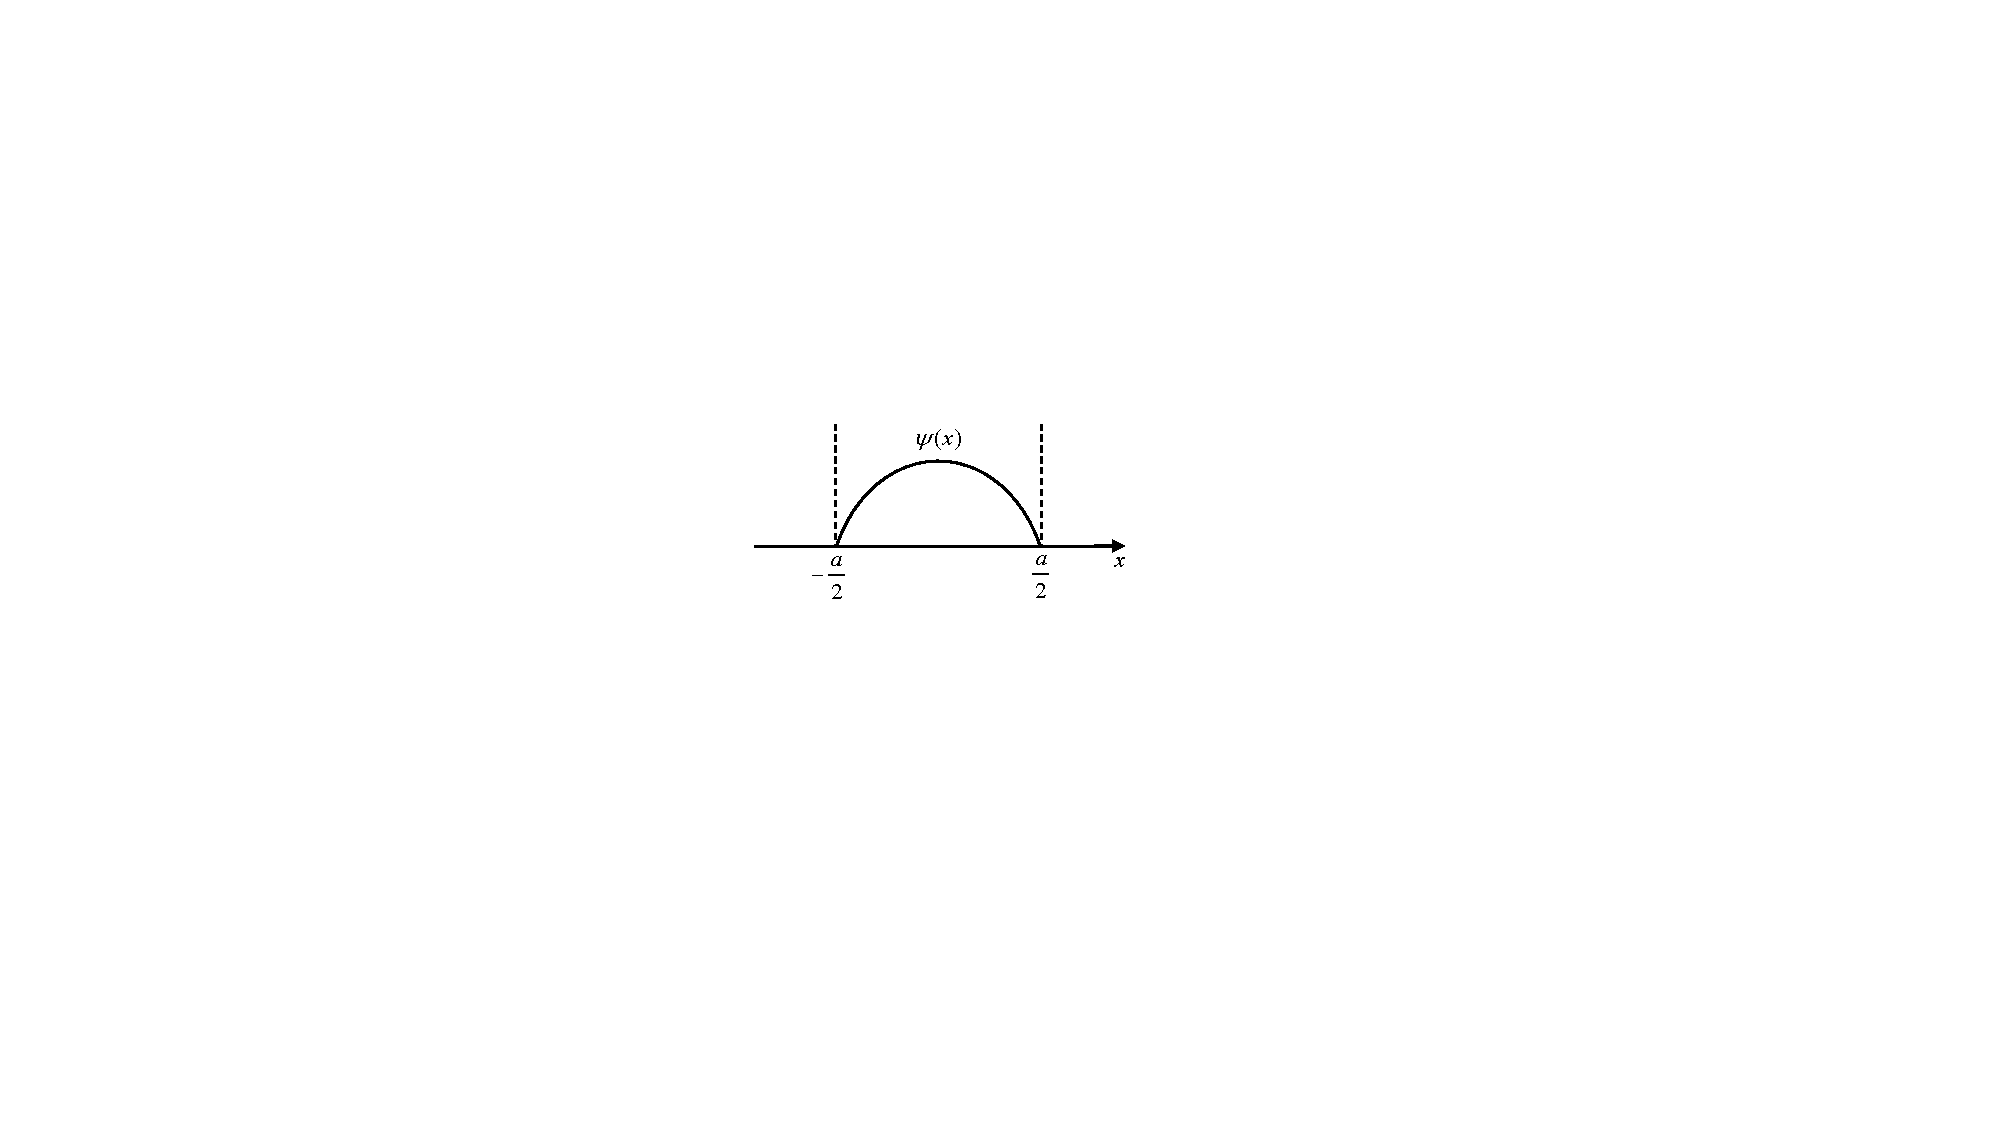
\includegraphics[width=3.5cm]{QM file/figure/3-1}
	\caption{}\label{fig.3-1}
\end{wrapfigure}

\example 如图\ref{fig.3-1},粒子在无限深势阱$\bigg(-\frac{a}{2}<x<\frac{a}{2}\bigg)$中运动,处于基态.如果突然破除势“墙”,而让粒子自由运动,粒子随即在一个方向(例如在$x>\frac{a}{2}$方向)被测量.设测得粒子动能在$(E,E+dE)$范围内的几率为$w(E)dE$,求$w(E)$.

\solution 势“墙”刚破除时,粒子的波函数$\varPsi(x)$就是势阱中的基态波函数,(波函数随时间的变化是连续的,不会突变.)根据\eqref{eq24.10}式,可知
\begin{empheq}{equation}\label{eq35.35}
	\varPsi(x)=
	\begin{dcases}
		\sqrt{\frac{2}{a}}\cos\frac{\pi x}{a},	& |x|<\frac{a}{2}	\\
		0,	& |x|>\frac{a}{2}
	\end{dcases}
\end{empheq}
势“墙”破除后,粒子将在全空间($-\infty<x<\infty$)自由运动.将$\varPsi(x)$展开成动量本征函数的线性叠加:
\begin{empheq}{equation}\label{eq35.36}
	\begin{aligned}
		\varPsi(x)&=\frac{1}{\sqrt{2\pi\hbar}}\int_{-\infty}^{\infty}C(p)e^{ipx/\hbar}dp	\\
		&=\frac{1}{\sqrt{2\pi}}\int_{-\infty}^{\infty}C(k)e^{ikx}dk
	\end{aligned}
\end{empheq}
其中
\begin{empheq}{equation}\label{eq35.37}
	p=\hbar k,\quad dp=\hbar dk,\quad C(k)=\sqrt{\hbar}C(p)
\end{empheq}
按照概率诠释,

$|C(k)|^{2}dk=|C(p)|^{2}dp=$粒子动量在$(p,p+dp)$范围内的概率,粒子自由运动时,能量(动能)和动量的关系是
\begin{empheq}{equation}\label{eq35.38}
	\begin{aligned}
			E	&=\frac{p^{2}}{2m}=\frac{\hbar^{2}k^{2}}{2m}	\\
		dE	&=\frac{\hbar^{2}kdk}{m}
	\end{aligned}
\end{empheq}
因此,
\begin{empheq}{equation*}
	w(E)dE=|C(k)|^{2}dk
\end{empheq}
\begin{empheq}{equation}\label{eq35.39}
	w(E)=|C(k)|^{2}\frac{dk}{dE}=\frac{m|C(k)|^{2}}{\hbar^{2}k}
\end{empheq}
可见关键是求出$C(k)$.按照\eqref{eq35.9}式及\eqref{eq35.37}式、\eqref{eq35.35}式,得
\begin{empheq}{equation}\label{eq35.40}
	\begin{aligned}
		C(k)&=\frac{1}{\sqrt{2\pi}}\int_{-\infty}^{\infty}\varPsi(x)e^{-ikx}dx	\\
		&=\frac{1}{\sqrt{\pi a}}\int_{-\frac{a}{2}}^{\frac{a}{2}}e^{-ikx}\cos\frac{\pi x}{a}dx	\\
		&=\sqrt{\frac{a}{\pi}}\bigg(\frac{1}{\pi-ak}+\frac{1}{\pi+ak}\bigg)\cos\frac{ak}{2}
	\end{aligned}
\end{empheq}
\begin{empheq}{equation}\label{eq35.41}
	|C(k)|^{2}=\frac{4\pi a}{(a^{2}k^{2}-\pi^{2})}\cos^{2}\frac{ak}{2}
\end{empheq}
$\dfrac{|C(k)|^{2}}{\hbar}$就是动量的概率分布函数$|C(p)|^{2}$,$|C(k)|^{2}$随$k$的变化如表\ref{lab.3-1}和图\ref{fig.3-2}所示

\begin{table}[!h]
	\begin{center}
		\caption{}\label{lab.3-1}
		\begin{tabular}{c|c|c|c|c|c|c|c|c}
			\hline 
			\multirow{2}{*}{$\dfrac{ka}{\pi}$} & \multirow{2}{*}{0} & \multirow{2}{*}{0.5} & \multirow{2}{*}{1} & \multirow{2}{*}{1.5} & \multirow{2}{*}{2} & \multirow{2}{*}{3} & \multirow{2}{*}{3.779} & \multirow{2}{*}{5} \\ 
			& & & & & & & & \\ \hline
			\multirow{2}{*}{$|C(k)|^{2}$} & \multirow{2}{*}{$\dfrac{4a}{\pi^{3}}$} & \multirow{2}{*}{$\dfrac{32a}{9\pi^{3}}$} & \multirow{2}{*}{$\dfrac{a}{4\pi}$} & \multirow{2}{*}{$\dfrac{32a}{25\pi^{3}}$} & \multirow{2}{*}{$\dfrac{4}{9\pi^{3}}$} & \multirow{2}{*}{0} & \multirow{2}{*}{\text{(极大)}} & \multirow{2}{*}{0} \\ 
			& & & & & & & & \\ \hline
			\multirow{2}{*}{$|\dfrac{C(k)}{C(0)}|^{2}$} & \multirow{2}{*}{1} & \multirow{2}{*}{$\dfrac{8}{9}$} & \multirow{2}{*}{$\dfrac{\pi^{2}}{16}$} & \multirow{2}{*}{$\dfrac{8}{25}$} & \multirow{2}{*}{$\dfrac{1}{9}$} & \multirow{2}{*}{0} & \multirow{2}{*}{0.005} & \multirow{2}{*}{0} \\ 
			& & & & & & & & \\ \hline
		\end{tabular}
	\end{center}
\end{table}

由图3-2可见,动量分布概率绝大部分集中在$|ka|<2\pi$范围内.如按下式粗略地规定(这样便于计算)分布半宽$\Delta k$,
\begin{empheq}{equation*}
	|C(0)|^{2}2\Delta k=\int_{-\infty}^{\infty}|C(k)|^{2}dk=1
\end{empheq}
则
\begin{empheq}{equation}\label{eq35.42}
	\frac{a}{\hbar}\Delta k=\frac{\pi^{2}}{8}=\num{1.23},\quad\Delta k=\num{1.23}\frac{\pi}{a}
\end{empheq}

\begin{figure}[!h]
	\centering
	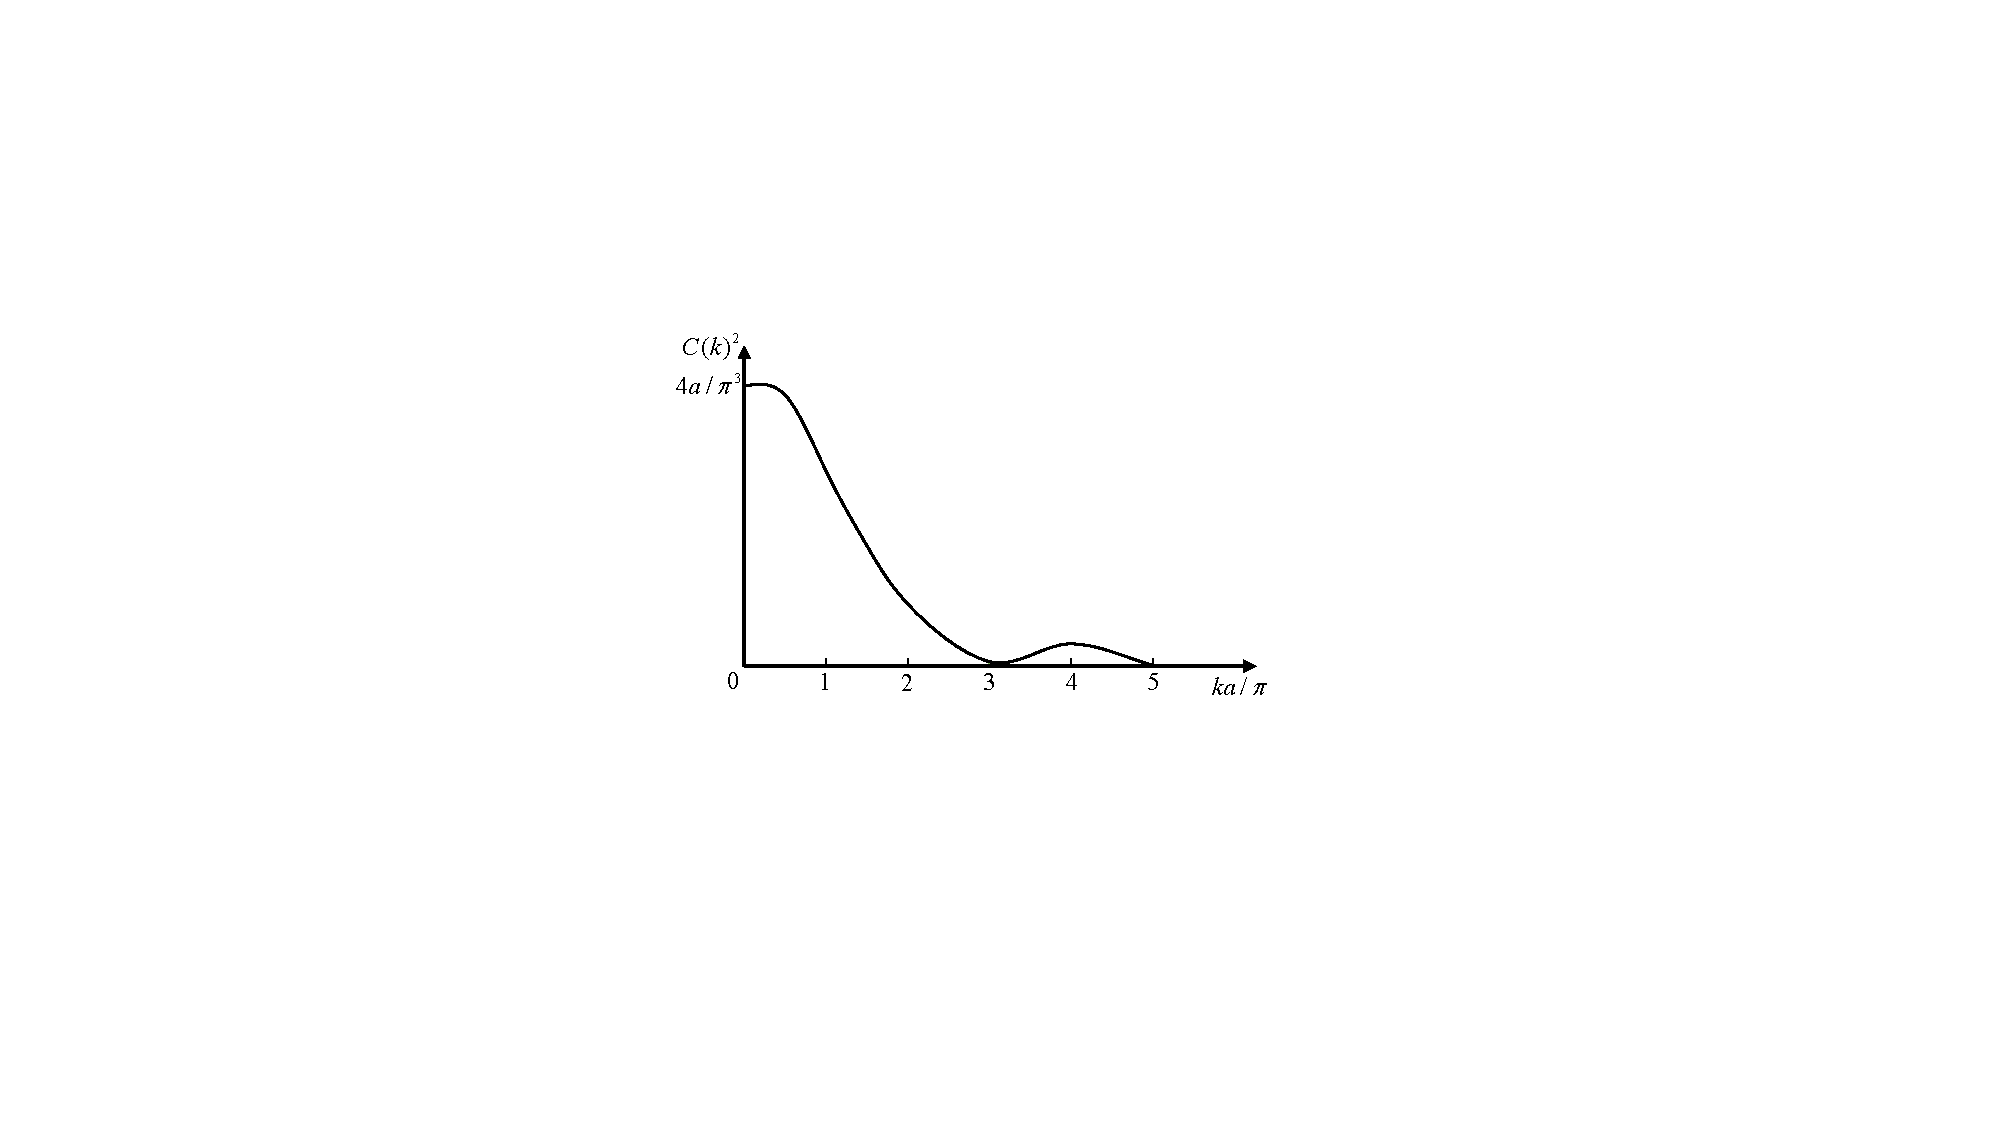
\includegraphics[width=5cm,clip]{QM file/figure/3-2}
	\caption{}\label{fig.3-2}
\end{figure}
$\Delta k$和波函数\eqref{eq35.35}式中的$k=\dfrac{\pi}{a}$很接近.

由\eqref{eq35.39}、\eqref{eq35.41}式求得粒子的动能概率分布函数为
\eqindent{5}
\begin{empheq}{equation}\label{eq35.43}
	\begin{aligned}
		w(E)&=\frac{m}{\hbar^{2}k}\frac{4\pi a}{(a^{2}k^{2}-\pi^{2})}\cos^{2}\frac{ak}{2}	\\
		&=\frac{1}{\hbar}\sqrt{\frac{m}{2E}}\frac{4\pi a}{\bigg(\frac{a^{2}}{\hbar^{2}}2mE-\pi^{2}\bigg)^{2}}\cos^{2}\frac{a}{\hbar}\sqrt{\frac{mE}{2}}
	\end{aligned}
\end{empheq}\eqnormal
用围道积分法不难验证:
\begin{empheq}{equation}\label{eq35.44}
	2\int_{0}^{\infty}w(E)dE=\int_{-\infty}^{\infty}|C(k)|^{2}dk=1
\end{empheq}



% 力学量算符的对易关系式
\section[力学量算符的对易关系式]{力学量算符的对易关系式} \label{sec:03.06} % 
% \makebox[5em][s]{} % 短题目拉间距

许多量子力学问题都涉及到力学蜇算符之间的对易关系式.最基本的就是位置算符和动量算符之间的对易关系式(见$\S$\ref{sec:03.02}):
\eqindent{10}
\begin{empheq}{align}	%1,2,3
	\hat{p_{x}}\hat{p_{y}}-\hat{p_{y}}\hat{p_{x}}=0	\label{eq36.1} \\%1
	\hat{x}\hat{p_{x}}-\hat{p_{x}}\hat{x}=i\hbar	\label{eq36.2} \\%2
	\hat{x}\hat{p_{y}}-\hat{p_{y}}\hat{x}=0			\label{eq36.3}	 %3
\end{empheq}
等等.为了便于运算,定义算符$\hat{A},\hat{B}$之间的对易式(又称量子括号):
\begin{empheq}{equation}\label{eq36.4}
	[\hat{A},\hat{B}]\equiv\hat{A}\hat{B}-\hat{B}\hat{A}
\end{empheq}\eqnormal
\eqindent{12}
则\eqref{eq36.1}、\eqref{eq36.2}、\eqref{eq36.3}式可以写成
\begin{empheq}{align*}	%1',2',3'
	[\hat{p_{x}},\hat{p_{y}}]&=0		\tag{$3.6.1^{\prime}$} \label{eq36.1'} \\
	[\hat{x}\hat{p_{x}}]&=i\hbar		\tag{$3.6.2^{\prime}$} \label{eq36.2'} \\
	[\hat{x}\hat{p_{y}}]&=0			\tag{$3.6.3^{\prime}$} \label{eq36.3'}
\end{empheq}\eqnormal
根据定义\eqref{eq36.4}式,容易证明以下运算规则:
\eqindent{6}
\begin{gather}
	[\hat{A},\hat{B}]=-[\hat{B},\hat{A}]	\label{eq36.5}\\ %5
	[\hat{A},\hat{B}+\hat{C}]=[\hat{A},\hat{B}]+[\hat{A},\hat{C}]	\label{eq36.6}\\ %6
	[\hat{A}+\hat{B},\hat{C}]=[\hat{A},\hat{C}]+[\hat{B},\hat{C}]	\label{eq36.7}\\ %7
	[\hat{A},\hat{B}\hat{C}]=[\hat{A},\hat{B}]\hat{C}+\hat{B}[\hat{A},\hat{C}]	\label{eq36.8}\\ %8
	[\hat{A}\hat{B},\hat{C}]=[\hat{A},\hat{C}]\hat{B}+\hat{A}[\hat{B},\hat{C}]	\label{eq36.9}\\ %9
	[\hat{A},[\hat{B},\hat{C}]]+[\hat{B}[\hat{C},\hat{A}]]+[\hat{C}[\hat{A},\hat{B}]]=0	\label{eq36.10} %10		
\end{gather}
熟练地掌握这些公式,计算就能进行得正确而迅速.例如利用\eqref{eq36.8}式及\eqref{eq36.2'}式,
可得
\begin{align}%11,12
	[\hat{x},\hat{p_{x}}^{2}] &=[\hat{x},\hat{p_{x}}]\hat{p_{x}}+\hat{p_{x}}[\hat{x},\hat{p_{x}}]=2i\hbar\hat{p_{x}}	\label{eq36.11}\\ %11
	[\hat{x},\hat{p_{x}}^{3}] &=[\hat{x},\hat{p_{x}}]\hat{p_{x}}^{2}+\hat{p_{x}}[\hat{x},\hat{p_{x}}^{2}]=3i\hbar\hat{p_{x}}^{2}	\label{eq36.12} %12
\end{align}\eqnormal
依此类推,对于任何正整数$n$,可证
\begin{empheq}{equation}\label{eq36.13}
	[\hat{x},\hat{p_{x}}^{n}]=i\hbar n\hat{p_{x}}^{n-1}=i\hbar\frac{\partial\hat{p_{x}}^{n}}{\partial\hat{p_{x}}}
\end{empheq}
再考虑到\eqref{eq36.3'}式,可知对于任何可以展开成$\hat{p_{x}},\hat{p_{y}},\hat{p_{z}}$正幕级数的算符$\hat{F(\boldsymbol{p})}$,有
下列对易关系式:
\begin{empheq}{equation}\label{eq36.14}
	[\hat{x},\hat{F(\boldsymbol{p})}]=i\hbar\frac{\partial\hat{F}}{\partial\hat{p_{x}}}
\end{empheq}
类似地,对于任意函数(作为算符)$f(\boldsymbol{r})$,有对易式
\begin{empheq}{equation}\label{eq36.15}
	[\hat{p_{x}},f(\boldsymbol{r})]=-i\hbar\frac{\partial f}{\partial x}
\end{empheq}

与轨道角动量算符$\hat{\boldsymbol{L}}=\boldsymbol{r}\times\boldsymbol{p}$有关的对易式应用极广,例如:
\eqindent{6}
\begin{empheq}{align}%16,17,18
	&[\hat{x},\hat{L_{x}}]=[\hat{x},\hat{y}\hat{p_{z}}]-[\hat{x},\hat{z}\hat{p_{y}}]=0	\label{eq36.16}\\
	&[\hat{x},\hat{L_{y}}]=[\hat{x},\hat{z}\hat{p_{x}}]-[\hat{x},\hat{x}\hat{p_{z}}]=\hat{z}[\hat{x},\hat{p_{x}}]=i\hbar\hat{z}	\label{eq36.17}\\
	&[\hat{L_{x}},\hat{y}]=[\hat{y}\hat{p_{z}},\hat{y}]-[\hat{z}\hat{p_{y}},\hat{y}]=-\hat{z}[\hat{p_{y}},\hat{y}]=i\hbar\hat{z}	\label{eq36.18}
\end{empheq}
类似地,可以证明
\begin{empheq}{equation}\label{eq36.19}
	[\hat{p_{x}},\hat{L_{x}}]=0,\quad[\hat{p_{x}},\hat{L_{y}}]=[\hat{L_{x}},\hat{p_{y}}]=i\hbar\hat{p_{z}}
\end{empheq}\eqnormal
等等.以上各式经过$(x\rightarrow y,y\rightarrow z,z\rightarrow x)$轮换后,仍旧成立.例如,\eqref{eq36.17}式和\eqref{eq36.18}式的轮换式是
\begin{empheq}{align*}
	[\hat{y},\hat{L_{z}}]=[\hat{L_{y}},\hat{z}]=i\hbar\hat{x}	\tag{$3.6.17^{\prime}$} \label{eq36.17'} \\
	[\hat{z},\hat{L_{x}}]=[\hat{L_{z}},\hat{x}]=i\hbar\hat{y}	\tag{$3.6.18^{\prime}$} \label{eq36.18'} 
\end{empheq}
\eqref{eq36.16}式的轮换式是
\begin{empheq}{equation*}\label{eq36.16'}
	[\hat{y},\hat{L_{y}}]=0,\quad [\hat{z},\hat{L_{z}}]=0	\tag{$3.6.16^{\prime}$} 
\end{empheq}

利用以上各式,就可以计算角动量算符$\hat{\boldsymbol{L}}$的各个分量之间的对易式,例如:
\eqindent{6}
\begin{empheq}{equation}\label{eq36.20}
	\begin{aligned}
		[\hat{L_{x}},\hat{L_{y}}]&=[\hat{y}\hat{p_{z}},\hat{L_{y}}]-[\hat{z}\hat{p_{y}},\hat{L_{y}}]	\\
		&=\hat{y}[\hat{p_{z}},\hat{L_{y}}]-[\hat{z},\hat{L_{y}}]\hat{p_{y}}	\\
		&=i\hbar(-\hat{y}\hat{p_{x}}+\hat{x}\hat{p_{y}})=i\hbar\hat{L_{z}}
	\end{aligned}
\end{empheq}\eqnormal
\eqref{eq36.20}式及其轮换式常被写成矢量形式:
\eqindent{12}
\begin{empheq}{equation}\label{eq36.21}
	\boxed{\hat{\boldsymbol{L}}\times\hat{\boldsymbol{L}}=i\hbar\hat{\boldsymbol{L}}}
\end{empheq}\eqnormal
利用\eqref{eq36.20}式或\eqref{eq36.21}式,可以进一步证明:
\begin{empheq}{equation}\label{eq36.22}
	[\hat{L_{\alpha}},\hat{\boldsymbol{L}}^{2}]=0,\quad \alpha=x,y,z
\end{empheq}
写成矢量形式,就是\eqindent{12}
\begin{empheq}{equation*}\label{eq36.22'}
	[\hat{\boldsymbol{L}},\hat{\boldsymbol{L}}^{2}]=0	\tag{$3.6.22^{\prime}$}
\end{empheq}\eqnormal
\eqref{eq36.21}、\eqref{eq36.22}式是角动蜇算符最本质的关系式.尤其是\eqref{eq36.21}式,是经典物理中根本不可能有的关系.在经典物理中,所有物理量都是普通数量,当然都是互相对易的,因此对于任何向量$\boldsymbol{A}$,总有$\boldsymbol{A}\times\boldsymbol{A}=0$.而作为量子力学算符的角动量$\hat{\boldsymbol{L}}$,各分量不对易,满足\eqref{eq36.21}式,由此决定了角动量的一系列异乎寻常的性质.$\S$\ref{sec:04.07}将详细讨论这个问题.

利用\eqref{eq36.16}至\eqref{eq36.19}式容易证明:
\begin{empheq}{equation}\label{eq36.23}
	[\hat{L_{\alpha}},\boldsymbol{r}^{2}]=0,\quad[\hat{L_{\alpha}},\hat{\boldsymbol{p}}^{2}]=0,\quad \alpha=x,y,z
\end{empheq}
亦即
\begin{empheq}{equation*}\label{eq36.23'}
	[\hat{\boldsymbol{L}},\boldsymbol{r}^{2}]=0,\quad [\hat{\boldsymbol{L}},\hat{\boldsymbol{p}}^{2}]=0	\tag{$3.6.23^{\prime}$}
\end{empheq}
利用$\hat{\boldsymbol{L}}$的球坐标表示式[\eqref{eq31.15}式],容易看出
\begin{empheq}{equation}\label{eq36.24}
	[\hat{\boldsymbol{L}},\hat{f(r)}]=0
\end{empheq}
$\hat{f(r)}$是任何径向函数(作为算符).总之,角动量算符$\hat{\boldsymbol{L}}$和任何标量(转动不变量)算符对易.

\example 选定任意两个空间方向,以$n,m$表示这两个方向的单位矢量:
\begin{empheq}{equation*}
	\boldsymbol{n}=(n_{x},n_{y},n_{z}),\quad\boldsymbol{m}=(m_{x},m_{y},m_{z})
\end{empheq}
定义角动量算符在$\boldsymbol{n},\boldsymbol{m}$方向的投影
\begin{empheq}{align*}
	\hat{L_{n}}&=\boldsymbol{n}\cdot\hat{\boldsymbol{L}}=n_{x}\hat{L_{x}}+n_{y}\hat{L_{y}}+n_{z}\hat{L_{z}}	\\
	\hat{L_{m}}&=\boldsymbol{m}\cdot\hat{\boldsymbol{L}}=m_{x}\hat{L_{x}}+m_{y}\hat{L_{y}}+m_{z}\hat{L_{z}}
\end{empheq}
试计算对易式$[\hat{L_{n}},\hat{L_{m}}]$.

\begin{wrapfigure}[6]{r}{7em}
	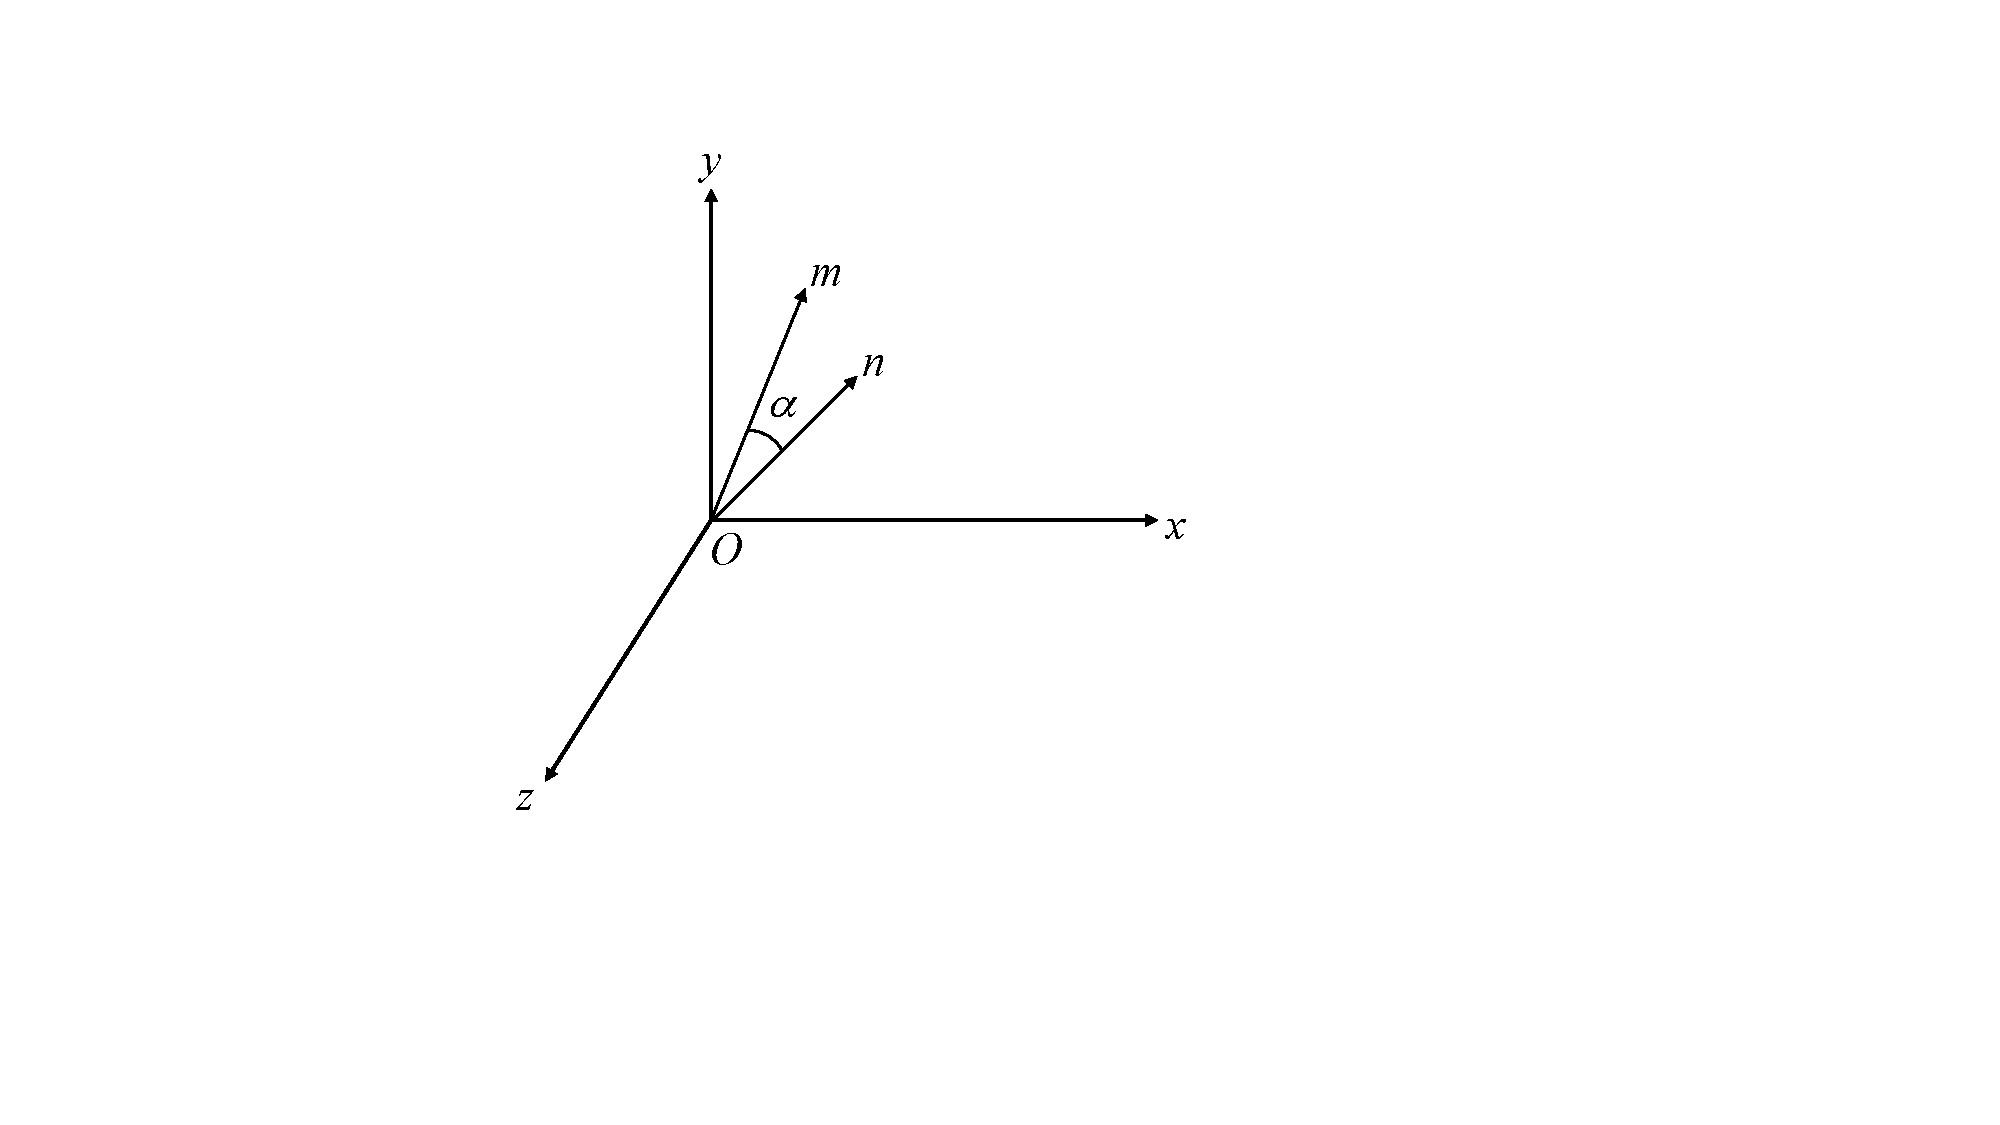
\includegraphics[width=3cm]{QM file/figure/3-3}
	\caption{}\label{fig.3-3}
\end{wrapfigure}

\solution 利用基本对易式\eqref{eq36.21},可得
\eqindent{2}
\begin{align}\label{eq36.25}
	[\hat{L_{n}},\hat{L_{m}}]& = n_{x}m_{y}[\hat{L_{x}},\hat{L_{y}}]+n_{y}m_{x}[\hat{L_{y}},\hat{L_{x}}]+\cdots	\nonumber\\
	&= (n_{x}m_{y}-n_{y}m_{x})i\hbar\hat{L_{z}}+\cdots	\nonumber\\
	&= i\hbar(\boldsymbol{n}\times\boldsymbol{m})_{z}\hat{L_{z}}+\cdots	\nonumber\\
	&= i\hbar(\boldsymbol{n}\times\boldsymbol{m})\cdot\hat{\boldsymbol{L}}
\end{align}\eqnormal
如以$\alpha$表示$(\boldsymbol{n},\boldsymbol{m})$夹角,$\boldsymbol{l}$表示$(\boldsymbol{n}\times\boldsymbol{m})$方向单位矢量,上式可以写成
\begin{empheq}{equation*}\label{eq36.25'}
	[\hat{L_{n}},\hat{L_{m}}]=i\hbar\hat{L_{l}}\sin\alpha
\end{empheq}
如果$\boldsymbol{n},\boldsymbol{m}$在$x-y$平面上,则$\boldsymbol{n}\times\boldsymbol{m}$指向$z$轴,如图\ref{fig.3-3}所示,上式成为
\begin{empheq}{equation}\label{eq36.26}
	[\hat{L_{n}},\hat{L_{m}}]=i\hbar\hat{L_{z}}\sin\alpha
\end{empheq}
其中角$\alpha$定义为由$\boldsymbol{n}$方向开始,沿逆时针方向转到$\boldsymbol{m}$方向所经历的角度($\alpha$可以大于$\pi$).





% 两个力学量算符的共同本征态
\section[两个力学量算符的共同本征态]{两个力学量算符的共同本征态} \label{sec:03.07} % 
% \makebox[5em][s]{} % 短题目拉间距

考虑物理体系(最简单的情况就是一个粒子)的两种力学量(可观测量)$A$,$B$.设在某种状态下,$A$和$B$都有确定的取值,$A=a_{n},B=b_{k}$.(为了叙述方便,设本征值谱是分立的)根据本征态和本征值的物理解释,可知这个状态既是算符$\hat{A}$的本征态,又是$\hat{B}$的本征态,亦即是$\hat{A}$和$\hat{B}$的共同本征态.相应的波函数记为$\varPsi_{nk}$,满足本征方程
\begin{empheq}{equation}\label{eq37.1}
	\hat{A}\varPsi_{nk}=a_{n}\varPsi_{nk},\quad \hat{B}\varPsi_{nk}=b_{k}\varPsi_{nk}
\end{empheq}
因此
\begin{empheq}{equation}\label{eq37.2}
	(\hat{A}\hat{B}-\hat{B}\hat{A})\varPsi_{nk}=(a_{n}b_{k}-b_{k}a_{n})\varPsi_{nk}=0
\end{empheq}
这结果提示我们,$\hat{A}$和$\hat{B}$可能是对易算符.但是,如$\hat{A},\hat{B}$仅存在个别的共同本征态,并不能由此得出$\hat{A},\hat{B}$是对易算符的结论.

如果$\hat{A},\hat{B}$存在一系列共同本征函数,构成完备函数系,情况就不同了.这时任何波函数$\varPsi$都可以表示成这些共同本征函数的线性叠加:
\begin{empheq}{equation}\label{eq37.3}
	\varPsi=\sum_{n,k}C_{nk}\varPsi_{nk}
\end{empheq}
从而
\begin{empheq}{equation*}
	(\hat{A}\hat{B}-\hat{B}\hat{A})\varPsi=\sum_{n,k}C_{nk}(\hat{A}\hat{B}-\hat{B}\hat{A})\varPsi_{nk}=0
\end{empheq}
由此可得
\begin{empheq}{equation}\label{eq37.4}
	\hat{A}\hat{B}-\hat{B}\hat{A}=[\hat{A},\hat{B}]=0
\end{empheq}
即$\hat{A},\hat{B}$为对易算符.

反过来,如果力学量算符$\hat{A},\hat{B}$对易,即$\hat{A}\hat{B}=\hat{B}\hat{A}$,则$\hat{A}$和$\hat{B}$必定存在一系列共同本征函数,并构成完全函数系证明如下.

由于$\hat{A}$和$\hat{B}$都是力学量算符,它们各自存在一组完备的本征函数系,记为$|\varPsi_{n}|$和$|\Phi_{k}|$,满足本征方程:
\begin{empheq}{align}%5,6
	\hat{A}\varPsi_{n}&=a_{n}\varPsi_{n},\quad n=1,2,3,\cdots	\label{eq37.5}\\
	\hat{B}\Phi_{k}&=b_{k}\Phi_{k},\quad k=1,2,3,\cdots	\label{eq37.5}
\end{empheq}
$n$和$k$为本征函数的编号数,对于简并态,本征值重复出现.任取一个$\hat{A}$的本征函数$\varPsi_{n}$,将它表示成$\hat{B}$的本征函数的线性叠加:
\begin{empheq}{equation}\label{eq37.7}
	\varPsi_{n}=\sum_{k}C_{nk}\Phi_{k}=\sum_{i}\tilde{\Phi_{i}}
\end{empheq}
考虑到可能存在的简并化,上式中$\tilde{\Phi_{i}}$表示$\sum_{k}$中相应于$\hat{B}$的同一个本征值$b_{i}$的各项之和(对于$\sum_{k}$中的非简并项,$\tilde{\Phi_{i}}$就是$C_{ni}\Phi_{i}$),因此
\begin{empheq}{equation}\label{eq37.8}
	\hat{B}\tilde{\Phi_{i}}=b_{i}\tilde{\Phi_{i}}
\end{empheq}
\eqref{eq37.7}式中各$\tilde{\Phi_{i}}$,相应于$\hat{B}$的不同本征值,因而是互相线性独立的.下面证明每个$\tilde{\Phi_{i}}$都是$\hat{A}$的本征函数.将\eqref{eq37.7}式代入\eqref{eq37.5}式,得到
\begin{empheq}{equation}\label{eq37.9}
	(\hat{A}-a_{n})\varPsi_{n}=\sum_{i}(\hat{A}-a_{n})\tilde{\Phi_{i}}=0
\end{empheq}
以算符$\hat{B}$作用于上式中每一项,由于$\hat{A},\hat{B}$对易,得到
\begin{empheq}{equation*}
	\hat{B}(\hat{A}-a_{n})\tilde{\Phi_{i}}=(\hat{A}-a_{n})\hat{B}\tilde{\Phi_{i}}=b_{i}(\hat{A}-a_{n})\tilde{\Phi_{i}}
\end{empheq}
上式表明,$(\hat{A}-a_{n})\tilde{\Phi_{i}}$如果不等于0,它就是$\hat{B}$的本征函数,相应于本征值$b_{i}$;而\eqref{eq37.9}式意味着相应于$\hat{B}$的不同本征值的本征函数是线性相关的!这当然是不可能的.为了避免这个矛盾,必须
\begin{empheq}{equation}\label{eq37.10}
	(\hat{A}-a_{n})\tilde{\Phi_{i}}=0
\end{empheq}
因此$\tilde{\Phi_{i}}$是$\hat{A}$的本征函数,相应于本征值$a_{n}$.至此已经证明了$\tilde{\Phi_{i}}$是$\hat{A},\hat{B}$的共同本征函数.这就是说,$\hat{A}$的每一个本征函数$\varPsi_{n}$都可以分解成若干个$\hat{A},\hat{B}$的共同本征函数$\tilde{\Phi_{i}}$.由于全体$|\varPsi_{n}|$是完备函数系,显然全体$\tilde{\Phi_{i}}$也是完备函数系.证明完毕.

从上面的论证可以得出一个直接的推论,即, 如$\hat{A},\hat{B}$对易, 而$\hat{A}$或$\hat{B}$具有某些非简并本征函数,则它们必然是$\hat{A},\hat{B}$的共同本征函数.

如果算符$\hat{A}$的全部本征函数都是非简并的,而算符$\hat{B}$和$\hat{A}$对易,则$\hat{A}$的每一个本征函数同时也是$\hat{B}$的本征函数,因此$\hat{B}$的本征值逐个取决于$\hat{A}$的本征值,从而可以认为力学量$B$是力学量$A$的函数.这样,凡是与$\hat{A}$对易的厄密算符,必定是$\hat{A}$的函数.如力学量$B$不是$A$的函数,则称$\hat{B}$独立于$\hat{A}$,显然$\hat{B}$和$\hat{A}$必定是不可对易的.

如果$\hat{A}$的一部分或全部本征函数是简并的,则给定$\hat{A}$的本征值并不足以完全确定波函数.这种情况下必然存在独立于$\hat{A}$而又与$\hat{A}$对易的其他力学量算符$\hat{B}$,它们存在共同本征函数,并构成完备函数系.如果$\hat{A},\hat{B}$的共同本征函数仍有简并,则给定$\hat{A},\hat{B}$的本征值仍不足以完全确定波函数,这时必定还存在独立于$\hat{A},\hat{B}$而又与$\hat{A},\hat{B}$对易的其他力学量算符.依此类推.

一组互相对易而又互相独立的力学量算符,如它们的共同本征函数是非简并的,并且构成完备函数系,则这组力学量称为力学量完全集,它们的一组本征值唯一地确定出一个共同本征态.构成完全集的独立力学量数目,称为物理体系的自由度.例如,一维谐振子,总能量算符$\hat{H}$的本征函数全部是非简并的,因此$H$本身就是力学量完全集,自由度为1.又如三维自由粒子,力学量完全集可以取为$(p_{x},p_{y},p_{z})$,总能量算符$\hat{H}=\hat{\boldsymbol{p}}^{2}/2m$是它们的函数,它们的共同本征函数$\varPsi_{\boldsymbol{p}}$[\eqref{eq35.10}式]就是通常说的平面波波函数;也可以选取别的力学量完全集,如$(\boldsymbol{p}^{2},\boldsymbol{L}^{2},L_{z})$,它们的共同本征态俗称自由粒子球面波,将在$\S$\ref{sec:05.02}讨论.

必须指出,两个或多个互不对易的力学量算符,也可能存在个别的共同本征函数,但是不足以构成完备函数系.设$\hat{A},\hat{B}$为力学量算符(厄密算符),不对易,设
\begin{empheq}{equation}\label{eq37.11}
	[\hat{A},\hat{B}]=\hat{A}\hat{B}-\hat{B}\hat{A}=i\hat{C}
\end{empheq}
容易证明$\hat{C}$是厄密算符.设$\varPsi_{ab}$是$\hat{A},\hat{B}$的共同本征函数,相应于本征值$A=a$,$B=b$.将\eqref{eq37.11}式作用于$\varPsi_{ab}$,易得
\begin{empheq}{equation}\label{eq37.12}
	\hat{C}\varPsi_{ab}=0
\end{empheq}
即$\varPsi_{ab}$也是算符$\hat{C}$的本征函数,本征值为0.所以,如果算符$\hat{C}$的本征值谱中不包含0,$\hat{A},\hat{B}$就没有共同本征函数.例如$\hat{A}=\hat{x},\hat{B}=\hat{p_{x}}$,$[\hat{x},\hat{p_{x}}]=i\hbar$,即$\hat{C}=\hbar$,$\hat{C}$的唯一本征值就是$\hbar$,所以$\hat{x}$和$\hat{p_{x}}$没有共同本征函数.注意,\eqref{eq37.12}式仅是$\hat{A},\hat{B}$的共同本征函数所必须满足的必要条件,并非充分条件.

\example 讨论轨道角动量$\boldsymbol{L}=\boldsymbol{r}\times\boldsymbol{p}$的任何两个分量存在共同本征函数的可能性,并求出这种共同本征函数.

\solution 算符$\hat{\boldsymbol{L}}$的三个分量互不对易,满足对易式:
\eqindent{4}
\begin{empheq}{equation}\label{eq37.13}
	[\hat{L_{x}},\hat{L_{y}}]=i\hbar\hat{L_{z}},\quad[\hat{L_{y}},\hat{L_{x}}]=i\hbar\hat{L_{x}},\quad[\hat{L_{z}},\hat{L_{x}}]=i\hbar\hat{L_{y}}
\end{empheq}\eqnormal
设$\varPsi$为$\hat{L_{x}}$,$\hat{L_{y}}$的共同本征征函数,以\eqref{eq37.13}第一式作用于$\varPsi$,得到
\begin{empheq}{equation}\label{eq37.14}
	\hat{L_{z}}\varPsi=0
\end{empheq}
再以\eqref{eq37.13}第二式和第三式作用于$\varPsi$,得到
\begin{empheq}{equation*}\label{eq37.14'}
	\hat{L_{x}}\varPsi=0,\quad\hat{L_{y}}\varPsi=0
\end{empheq}
所以,$\hat{\boldsymbol{L}}$的任何两个分量的共同本征函数,必为三个分量的共同本征函数,本征值全部等于0,亦即$\varPsi$满足
\begin{empheq}{equation}\label{eq37.15}
	\hat{\boldsymbol{L}}\varPsi=-i\hbar\boldsymbol{r}\times\nabla\varPsi=0
\end{empheq}
因此$\nabla\varPsi$的方向和$\boldsymbol{r}$平行.满足这条件的$\varPsi$必须是径向函数,即
\begin{empheq}{equation}\label{eq37.16}
	\varPsi=\varPsi(r)\quad\text{(与$\theta,\varphi$无关)}
\end{empheq}
这就是$\hat{\boldsymbol{L}}$的三个分量的共同本征函数.显然,\eqref{eq37.16}式并不构成完全函数系,它不
能表示与方向$(\theta,\varphi)$有关的波函数.














% 不确定度关系
\section[不确定度关系]{不确定度关系} \label{sec:03.08} % 
% \makebox[5em][s]{} % 短题目拉间距

考虑两个力学量$A,B$及其算符$\hat{A},\hat{B}$,任意给定一个归一化的波函数$\varPsi$.如$\varPsi$是$\hat{A}$或$\hat{B}$的本征函数,则力学量$A$或$B$将取单一的本征值,这种情况不予讨论.如$\varPsi$不是$\hat{A}$或$\hat{B}$的本征函数,则$A$和$B$的取值均将具有某种分布,定义分布宽度(涨落)$\Delta A$,$\Delta B$,
\begin{empheq}{equation}\label{eq38.1}
	\begin{aligned}
		(\Delta A)^{2}&=\overline{(\hat{A}-\bar{A})^{2}}=\overline{A^{2}}-\bar{A}^{2}	\\
		(\Delta B)^{2}&=\overline{(\hat{B}-\bar{B})^{2}}=\overline{B^{2}}-\bar{B}^{2}
	\end{aligned}
\end{empheq}
试问,对于各种不同的波函数$\varPsi$,$\Delta A\cdot\Delta B$的下限是什么?如果$\hat{A},\hat{B}$对易,可取$\varPsi$尽量接近$\hat{A},\hat{B}$的共同本征函数,使$\Delta A,\Delta B$都很小,所以$\Delta A\cdot\Delta B$的下限为0.如$\hat{A},\hat{B}$不对易,令
\begin{empheq}{equation}\label{eq38.2}
	[\hat{A},\hat{B}]\equiv\hat{A}\hat{B}-\hat{B}\hat{A}=i\hat{C}
\end{empheq}
$\hat{C}$必为厄密算符,它在$\varPsi$态下的平均值
\begin{empheq}{equation}\label{eq38.3}
	\bar{C}=-i\int\varPsi^{*}(\hat{A}\hat{B}-\hat{B}\hat{A})\varPsi d\tau
\end{empheq}
必为实数,可以证明
\begin{empheq}{equation}\label{eq38.4}
	\boxed{\Delta A\cdot\Delta B\geqslant\frac{1}{2}|\bar{C}|}
\end{empheq}
称为不确定度关系(曾称为测不准关系).\eqref{eq38.4}式的证明如下.

对于任意线性算符$\hat{F}$及其共轭$\hat{F}^{*}$,$\hat{F}^{*}\hat{F}$的平均值为
\eqindent{6}
\begin{empheq}{align}\label{eq38.5}
	\overline{\hat{F}^{*}\hat{F}}&=\int\varPsi^{*}\hat{F}^{*}\hat{F}\varPsi d\tau	\nonumber\\
	&=\int(\hat{F}\varPsi)(\hat{F}\varPsi)^{*}d\tau=\int|\hat{F}\varPsi|^{2}d\tau\geqslant 0
\end{empheq}\eqnormal
令
\begin{empheq}{equation}\label{eq38.6}
	\hat{F}=\hat{A}+i\xi\hat{B}
\end{empheq}
$\xi$为实参数(注意,如$A,B$量纲相同,$\xi$是无量纲参数;如$A,B$量纲不同,则$\xi$有量纲.)
\eqindent{6}
\begin{empheq}{align}\label{eq38.7}
	\hat{F}^{*}\hat{F}&=(\hat{A}-i\xi\hat{B})(\hat{A}+i\xi\hat{B})	\nonumber\\
		&=\hat{A}^{2}+\xi^{2}\hat{B}^{2}+i\xi[\hat{A},\hat{B}]=\hat{A}^{2}+\xi^{2}\hat{B}^{2}-\xi\hat{C}
\end{empheq}\eqnormal
代入\eqref{eq38.5}式, 即得
\begin{empheq}{equation}\label{eq38.8}
	\overline{A^{2}}+\xi^{2}\overline{B^{2}}-\xi\overline{C}\geqslant 0
\end{empheq}
等号成立的条件为
\begin{empheq}{equation}\label{eq38.9}
	\hat{F}\varPsi=(\hat{A}+i\xi\hat{B})\varPsi=0
\end{empheq}
\eqref{eq38.8}式对任何$\xi$值(实数),任何归一化波函数$\varPsi$,均可成立.但如$\varPsi$是$\hat{A}$或$\hat{B}$的本征函数,这时$\bar{C}=0$,\eqref{eq38.8}式没有实际价值.

\eqref{eq38.8}式中取$\xi=\pm 1$(如$\bar{C}>0$,取$\xi=1$;如$\bar{C}<0$,取$\xi=-1$)得到
\begin{empheq}{equation}\label{eq38.10}
	\overline{A^{2}}+\overline{B^{2}}\geqslant|\bar{C}|
\end{empheq}
\eqref{eq38.8}式中取$\xi=\bar{C}/(2\overline{B^{2}})$或$\xi=\pm\sqrt{\overline{A^{2}}/\overline{B^{2}}}$($\bar{C}>0$,取正号;$\bar{C}<0$,取负号),得到
\begin{empheq}{equation}\label{eq38.11}
	\overline{A^{2}}\overline{B^{2}}\geqslant\frac{1}{4}\bar{C}^{2}
\end{empheq}
这实际上是\eqref{eq38.8}式成立的充要条件.\eqref{eq38.11}式其实已经包含了\eqref{eq38.10}式.

\eqref{eq38.8}至\eqref{eq38.11}式适用于任何厄密算符$\hat{A},\hat{B}$.如将$\hat{A}$换成$(\hat{A}-\bar{A})$,$\hat{B}$换成$(\hat{B}-\bar{B})$,则
\begin{empheq}{align*}
	[\hat{A}-\bar{A},\hat{B}-\bar{B}]=[\hat{A},\hat{B}]=i\hat{C}	\\
	\overline{(\hat{A}-\bar{A})^{2}}=(\Delta A)^{2},\quad\overline{(\hat{B}-\bar{B})^{2}}=(\Delta B)^{2} 
\end{empheq}
\eqref{eq38.10}式换成
\begin{empheq}{equation}\label{eq38.12}
	(\Delta A)^{2}+(\Delta B)^{2}\geqslant|\bar{C}|=|\overline{AB-BA}|
\end{empheq}
注意,\eqref{eq38.10}式和\eqref{eq38.12}式仅适用于$A,B$量纲相同的情形.\eqref{eq38.11}式换成
\begin{empheq}{equation*}
	\Delta A\cdot\Delta B\geqslant\frac{1}{2}|\bar{C}|=\frac{1}{2}|\overline{AB-BA}|
\end{empheq}
这就是不确定度关系\eqref{eq38.4}式成立,\eqref{eq38.12}式必然成立.

狭义的不确定度关系是指$A=x,B=p_{x}$的情形,这时
\begin{empheq}{equation*}
	[x,p_{x}]=i\hbar
	\tag{$3.8.4$}
\end{empheq}
相当于$\hat{C}=\hbar$,这时\eqref{eq38.11}式和\eqref{eq38.4}式变成
\begin{empheq}{equation}\label{eq38.13}
	\overline{x^{2}}\overline{p_{x}^{2}}\geqslant\frac{\hbar^{2}}{4}
\end{empheq}
\begin{empheq}{equation}\label{eq38.14}
	\boxed{\Delta x\cdot\Delta p_{x}\geqslant\frac{\hbar}{2}}
\end{empheq}
历史上, 不确定关系是海森堡(W. Heisenberg)首先提出来的.海森堡分析了若干典型实验后指出,微观粒子的位置和动量不可能同时予以精确测定,而只能确定到(在量级的意义上)
\begin{empheq}{equation*}
	\Delta x\cdot\Delta p\gtrsim h
\end{empheq}
的程度.\eqref{eq38.14}式则是严格的定量结果.注意,\eqref{eq38.14}式只规定了$\Delta x\cdot\Delta p_{x}$的下限,并未规定出上限.对许多典型定态问题的计算结果表明,对于多数问题的基态,$\Delta x\Delta p_{x}$接近于$\hbar$;而对于高激发态,$\Delta x\Delta p_{x}$的值可以很大.例如,一维谐振子的基态$\varPsi_{0}$,$\Delta x\Delta p_{x}=\frac{\hbar}{2}$,刚好是\eqref{eq38.14}式的下限;对于$\varPsi_{n}$态,$\Delta x\Delta p_{x}=\bigg(n+\frac{1}{2}\bigg)\hbar$.

不确定度关系集中反映了量子力学规律的特点,规定了经典力学轨道概念的适用限度.例如,经典力学认为质点有绝对静止状态,位置完全确定($\Delta x=0$),动量为0.而按照不确定度关系\eqref{eq38.14},这种经典静止状态是不可能的.实验事实正是这样,粒子的位置越确定($\Delta x$小),动量的涨落$\Delta p$就越大,动能的数值也越大(参看下面的例题).又如经典力学认为质点均有运动轨道,在任何时刻质点均有明确的位置和动量,$\Delta x=0,\Delta p_{x}=0$.而不确定关系\eqref{eq38.14}告诉我们, 在任何时刻粒子的$\Delta x$与$\Delta p_{x}$之积不小于$\frac{\hbar}{2}$,这就根本否定了轨道运动的概念.但是,在\eqref{eq38.14}式的限制下,如果$\Delta x$和$\Delta p_{x}$实际上都很小,可以忽略不计,则轨道概念仍可近似成立.例如电子在宏观尺度上运动,$x$的量级如取为厘米,如果$\Delta x\sim 10^{-4}\si{cm}$,这是不易观测到的,按照\eqref{eq38.14}式,$\Delta p_{x}$的下限为
\begin{empheq}{equation*}
	\Delta p_{x}\sim\frac{\hbar}{\Delta x}\sim 10^{-28}\si{kg\cdot m\cdot s^{-1}}
\end{empheq}
如果电子的动能等于1\si{eV},则动量等于
\begin{empheq}{equation*}
	p=\sqrt{2m_{e}E}\sim \num{5.4}\times 10^{-25}\si{kg\cdot m\cdot s^{-1}}
\end{empheq}
和$p$相比,$\Delta p_{x}$也是微不足道的,因此轨道概念可以近似成立,电子的宏观运动可以用经典力学来处理.电子在原子范围内运动,情况就完全不同了,这时电子的位置(从原子核处算起)的量级约为
\begin{empheq}{equation*}
	x\sim a_{0}\sim\num{0.53}\times 10^{-10}\si{m}\text{(玻尔半径)}
\end{empheq}
电子的动能盐级约为10\si{eV},因此
\begin{empheq}{equation*}
	p\sim \sqrt{2m_{e}\times10\si{eV}}\sim 1.7\times10^{-24}\si{kg\cdot m\cdot s^{-1}}	
\end{empheq}
\begin{empheq}{equation*}
	x\cdot p\sim 8.5\times 10^{-35} \si{J\cdot s}\sim\hbar	
\end{empheq}
由于\eqref{eq38.14}式的限制,已经不可能同时使$\Delta x\ll x,\Delta p\ll p$,亦即经典轨道的概念不再适用.

\example 用不确定度关系估算原子核中核子(质子,中子)动能的量级,并解释电子不可能是原子核的结构单元.

\solution 中等大小的原子核,半径$R$约为5\si{fm}左右.核子在核内的分布基本上是均匀的,就一个核子来说,
\begin{empheq}{equation*}
	\overline{r^{2}}\approx\frac{1}{\tau}\int_{\tau}r^{2}d\tau=\frac{4\pi}{4\pi R^{3}/3}\int_{0}^{R}r^{4}dr=\frac{3}{5}R^{2}	
\end{empheq}
\begin{empheq}{equation*}
	\overline{x^{2}}\approx\frac{1}{3}\overline{r^{2}}\approx\frac{1}{5}R^{2}	
\end{empheq}
对于全体核子的总平均,可取
\begin{empheq}{equation*}
	\overline{p_{x}^{2}}\sim\frac{\hbar^{2}}{x^{2}}\sim\frac{5\hbar^{2}}{R^{2}}	
\end{empheq}
\begin{empheq}{equation*}
	\overline{p^{2}}\sim3\overline{p_{x}^{2}}\sim\frac{15\hbar^{2}}{R^{2}}	
\end{empheq}
核子平均动能约为
\begin{empheq}{equation*}
	\frac{\overline{p^{2}}}{2m_{p}}\sim\frac{15\hbar^{2}}{2m_{p}R^{2}}=\frac{15\hbar^{2}c^{2}}{2m_{p}c^{2}R^{2}}\sim 12\si{MeV}	
\end{empheq}
核子动能的实验值约为$10\sim 20$\si{MeV}.

如果设想原子核的结构单元中也有电子,则电子的动量估计值仍如上述,$p^{2}\sim\frac{15\hbar^{2}}{R^{2}}$,如用公式$\frac{p^{2}}{2m_{e}}$计算动能,则
\begin{empheq}{equation*}
	\frac{p^{2}}{2m_{e}}\sim\frac{m_{p}}{m_{e}}\times 12 \si{MeV}\sim 2.2\times 10^{4} \si{MeV}
\end{empheq}
远大于$m_{e}c^{2}$.这种情况下应该用相对论公式,
\begin{empheq}{equation*}
	E\sim pc \sim\sqrt{15}\frac{\hbar c}{R}\sim 150\si{MeV}
\end{empheq}
欲将动能这么大的电子束缚在原子核中,需要量级相同的负的势能.但是能够吸引电子的只有质子-电子间的库仑吸引力,其势能约为
\begin{empheq}{equation*}
	V\sim -\frac{Ze^{2}}{R}\quad \text{(Z:核内质子总数)}
\end{empheq}
如取$Z\sim40$,则$V\sim-12\si{MeV}$,数值远小于动能估计值150\si{MeV}.由此可见,电子不可能是原子核的结构单元.

事实上,原子核发生$\beta^{-}$衰变时,临时产生出来的电子,其动能最多只有几个\si{MeV},其德布罗意波长
\begin{empheq}{equation*}
	\lambda=\frac{h}{p}\sim\frac{hc}{E}\sim\frac{1.24\times 10^{3}\si{MeV}\cdot\si{fm}}{E}
\end{empheq}
$\lambda$远大于核半径,所以$\beta^{-}$电子不可能在核内久留,几乎立刻逸出核外.






% 状态和力学量随时间的变化
\section[状态和力学量随时间的变化]{状态和力学量随时间的变化} \label{sec:03.09} % 
% \makebox[5em][s]{} % 短题目拉间距

{\heiti 1. 波函数随时间的变化}

波函数$\varPsi$随时间的变化取决于薛定谔方程
\begin{empheq}{equation}\label{eq39.1}
	i\hbar\frac{\partial}{\partial t}\varPsi(\boldsymbol{r},t)=\hat{H}\varPsi(\boldsymbol{r},t)
\end{empheq}
$\hat{H}$为哈密顿算符.如$\hat{H}$与时间$t$无关,$\hat{H}$就是总能量算符.在以下的讨论中,均设$\hat{H}$与$t$无关.设$\hat{H}$的本征函数,本征值为$|\varPsi_{n}(\boldsymbol{r},E_{n})|$,满足本征方程
\begin{empheq}{equation}\label{eq39.2}
	\hat{H}\varPsi_{n}=E_{n}\varPsi_{n},\quad n=1,2,\cdots
\end{empheq}
\eqref{eq39.1}式是时间$t$的一阶微分方程,只需给定初始时刻$(t_{0}=0)$的波函数$\varPsi(\boldsymbol{r},0)$,就可以解出所有时刻的波函数$\varPsi(\boldsymbol{r},t)$.具体说来,先将$\varPsi(\boldsymbol{r},0)$表示成各$\varPsi_{n}(\boldsymbol{r})$的线性叠加,
\begin{empheq}{equation}\label{eq39.3}
	\varPsi(\boldsymbol{r},0)=\sum_{n}C_{n}\varPsi_{n}(\boldsymbol{r})
\end{empheq}
其中
\begin{empheq}{equation}\label{eq39.4}
	C_{n}=\int\varPsi_{n}^{*}(\boldsymbol{r})\varPsi(\boldsymbol{r},0)d\tau
\end{empheq}
以\eqref{eq39.3}式作为初始条件,容易求出\eqref{eq39.1}式的解为[参看\eqref{eq21.21}式]
\begin{empheq}{equation}\label{eq39.5}
	\varPsi(\boldsymbol{r},0)=\sum_{n}C_{n}e^{E_{n}t/(i\hbar)}\varPsi_{n}(\boldsymbol{r})
\end{empheq}
利用本征方程\eqref{eq39.2}以及\eqref{eq39.3}式,可将\eqref{eq39.5}式化成
\begin{empheq}{align}\label{eq39.6}
	\varPsi(\boldsymbol{r},t) &=\sum_{n}C_{n}e^{\hat{H}t/(i\hbar)}\varPsi_{n}(\boldsymbol{r})	\nonumber\\
	&=e^{\hat{H}t/(i\hbar)}\varPsi(\boldsymbol{r},0)=\hat{U}(t)\varPsi(\boldsymbol{r},0)
\end{empheq}
其中
\begin{empheq}{equation}\label{eq39.7}
	\hat{U}(t)=e^{\hat{H}t/(i\hbar)}\equiv\sum_{\nu=0}^{\infty}\frac{1}{\nu!}\bigg(\frac{\hat{H}t}{i\hbar}\bigg)^{\nu}
\end{empheq}
称为演化算符.\eqref{eq39.6}式表明,演化算符$\hat{U}(t)$作用于初始时刻的波函数,就得到$t$时刻的波函数.注意$\hat{U}(0)=1$.$\hat{U}(t)$不是厄密算符,其共轭为
\begin{empheq}{equation}\label{eq39.8}
	\hat{U}^{*}(t)=e^{-\hat{H}t/(i\hbar)}
\end{empheq}
因此
\begin{empheq}{equation}\label{eq39.9}
	\hat{U}^{*}(t)\hat{U}(t)=\hat{U}(t)\hat{U}^{*}(t)=1
\end{empheq}
亦即$\hat{U}(t)$是一种么正变换.注意$\hat{U}(t)$和$\hat{U}^{*}(t)$均与$\hat{H}$对易,其变化率为
\begin{empheq}{equation}\label{eq39.10}
	\begin{aligned}
		\frac{\partial\hat{U}(t)}{\partial t}=\frac{1}{i\hbar}\hat{H}\hat{U}(t)=\frac{1}{i\hbar}\hat{U}(t)\hat{H}	\\
		\frac{\partial^{*}\hat{U}(t)}{\partial t}=\frac{1}{i\hbar}\hat{H}\hat{U}^{*}(t)=\frac{1}{i\hbar}\hat{U}^{*}(t)\hat{H}
	\end{aligned}
\end{empheq}

{\heiti 2. 力学量平均值随时间的变化}

量子力学中力学量的变化率不能仿照经典力学的方式来定义,在经典力学中,处于某种运动状态的质点,任何力学量$F(t)$在任何时刻$t$均有明确的数值,而且随$t$作连续变化,所以可以定义$F$的时间变化率为
\begin{empheq}{equation*}
	\frac{dF(t)}{dt}=\lim_{\Delta\rightarrow 0}\frac{F(t+\Delta t)-F(t)}{\Delta t}
\end{empheq}
量子力学则不同.我们来讨论在任意运动态$\varPsi(\boldsymbol{r},t)$下某个力学量$A(\boldsymbol{r,p})$的取值问题.首先,一般来说,在任意时刻$t$,力学量$A$的取值不是唯一的,可以取多种本征值(各有某种几率).其次,即使在某个特定时刻$t_{0}$,$\varPsi(\boldsymbol{r},t_{0})$刚好是$\hat{A}$的本征态,因而这时$A$取单一的本征值,但在随后的时刻,由于波函数按照薛定谔方程随时间变化,$\varPsi(\boldsymbol{r},t_{0}+\Delta t)$一般就不再是$\hat{A}$的本征态,因此在时刻$t_{0}+\Delta t$,$A$将取多种本征值这样,当然就谈不上力学量$A$的取值随时间作连续变化.所以经典力学量的变化率定义在量子力学中完全不适用.

在量子力学中,力学量$A(\boldsymbol{r,p})$在运动态$\varPsi(\boldsymbol{r},t)$下的平均值为
\begin{empheq}{equation}\label{eq39.11}
	\bar{A}(t)=\int\varPsi^{*}(\boldsymbol{r},t)\hat{A}\varPsi(\boldsymbol{r},t)d\tau
\end{empheq}
由于$\varPsi$随$t$作连续变化,所以$\bar{A}$亦随$t$作连续变化.力学量$A$的变化率算符$\frac{d\hat{A}}{dt}$按照下述方式定义:$\frac{d\hat{A}}{dt}$在运动态$\varPsi(\boldsymbol{r},t)$下的平均值等于$\\bar{A}(t)$的变化率,亦即
\eqindent{1}
\begin{empheq}{equation}\label{eq39.12}
	\frac{\overline{dA}}{dt}\equiv\int\varPsi^{*}(\boldsymbol{r},t)\frac{d\hat{A}}{dt}\varPsi(\boldsymbol{r},t)d\tau=\frac{d}{dt}\int\varPsi^{*}(\boldsymbol{r},t)\hat{A}\varPsi(\boldsymbol{r},t)d\tau=\frac{d}{dt}\overline{A}(t)
\end{empheq}\eqnormal
利用演化算符$\hat{U}(t)$,\eqref{eq39.11}式可以化成
\eqindent{6}
\begin{empheq}{align}\label{eq39.13}
	\overline{A}(t) &=\int\{\hat{U}(t)\varPsi(\boldsymbol{r},0)\}^{*}\hat{A}\hat{U}(t)\varPsi(\boldsymbol{r},0)d\tau\nonumber	\\
	&=\int\varPsi^{*}(\boldsymbol{r},0)\hat{U}^{+}(t)\hat{A}\hat{U}(t)\varPsi(\boldsymbol{r},0)d\tau
\end{empheq}\eqnormal
利用\eqref{eq39.10}式,不难求出
\eqindent{4}
\begin{empheq}{align}\label{eq39.14}
	\frac{d\overline{A}(t)}{dt}
	&=\int\varPsi^{*}(\boldsymbol{r},0)
	\biggl\{\frac{\partial}{\partial t}\hat{U}^{*}(t)\hat{A}\hat{U}(t)\biggr\}
	\varPsi(\boldsymbol{r},0)d\tau	\nonumber\\
	&=\frac{1}{i\hbar}\int\varPsi^{*}(\boldsymbol{r},0)\hat{U}^{+}(t)(\hat{A}\hat{H}-\hat{H}\hat{A})\hat{U}(t)\varPsi(\boldsymbol{r},0)d\tau	\nonumber\\
	&=\frac{1}{i\hbar}\int\{\hat{U}(t)\varPsi(\boldsymbol{r},0)\}^{*}(\hat{A}\hat{H}-\hat{H}\hat{A})\hat{U}(t)\varPsi(\boldsymbol{r},0)d\tau	\nonumber\\
	&=\frac{1}{i\hbar}\int\varPsi^{*}(\boldsymbol{r},t)(\hat{A}\hat{H}-\hat{H}\hat{A})\hat{U}(t)\varPsi(\boldsymbol{r},t)d\tau	\nonumber\\
	&=\frac{1}{i\hbar}\overline{(AH-HA)}=\frac{1}{i\hbar}\overline{[\hat{A},\hat{H}]}
\end{empheq}\eqnormal
亦即
\begin{empheq}{equation}\label{eq39.15}
	\boxed{\frac{d\hat{A}}{dt}=\frac{1}{i\hbar}[\hat{A},\hat{H}]}
\end{empheq}
在\eqref{eq39.14}式的推导过程中,并没有用到$\hat{A}$是厄密算符$(\hat{A}^{*}=\hat{A})$这个条件.所以,对于非厄密算符$(\hat{A}^{*}\neq\hat{A})$,仍可将\eqref{eq39.11}式作为其平均值的定义,\eqref{eq39.12}式作为其变化率算符的定义,结果仍得到\eqref{eq39.14}、\eqref{eq39.15}式.

如果$\hat{A},\hat{H}$对易,即$[\hat{A},\hat{H}]$,则$\frac{d\hat{A}}{dt}=0,\frac{d\bar{A}}{dt}=0$,力学量$A$称为守恒量.当$\hat{H}$不显含$t$时,$H$就是守恒量,即能量守恒.

\eqref{eq39.15}式也称力学量算符的运动方程.下面就
\begin{empheq}{equation}\label{eq39.16}
	\hat{H}=\frac{\hat{\boldsymbol{p}}^{2}}{2m}+V(\boldsymbol{r})
\end{empheq}
的情形,具体求出基本力学量算符的运动方程.先求位置$r$的运动方程,
\begin{empheq}{equation}\label{eq39.17}
	\frac{d\hat{x}}{dt}=\frac{1}{i\hbar}[\hat{x},\hat{H}]=\frac{1}{i\hbar 2m}[\hat{x},\hat{\boldsymbol{p}^{2}}]=\frac{\hat{p_{x}}}{m}
\end{empheq}
类似地,求得
\begin{empheq}{equation*}\label{eq39.17'}
	\frac{d\hat{y}}{dt}=\frac{\hat{p_{y}}}{m},\quad\frac{d\hat{z}}{dt}=\frac{\hat{p_{z}}}{m}	\tag{$3.9.17^{\prime}$}
\end{empheq}
写成矢量形式,就是
\begin{empheq}{equation*}\label{eq39.17''}
	\frac{d\hat{\boldsymbol{r}}}{dt}=\frac{\hat{\boldsymbol{r}}}{m}	\tag{$3.9.17^{\prime\prime}$}
\end{empheq}
这公式相当于经典力学中速度的定义,再看动量,
\begin{empheq}{equation}\label{eq39.18}
	\frac{d\hat{p_{x}}}{dt}=\frac{1}{i\hbar}[\hat{p_{x}},\hat{H}]=\frac{1}{i\hbar}[\hat{p_{x}},V]=-\frac{\partial V}{\partial x}
\end{empheq}
类似地,求得
\begin{empheq}{equation*}\label{eq39.18'}
	\frac{d\hat{p_{y}}}{dt}=-\frac{\partial V}{\partial y},\quad\frac{d\hat{p_{z}}}{dt}=-\frac{\partial V}{\partial z}	\tag{$3.9.18^{\prime}$}
\end{empheq}
写成矢量形式,就是
\begin{empheq}{equation*}\label{eq39.18''}
	\frac{d\hat{\boldsymbol{p}}}{dt}=0=-\nabla V=\boldsymbol{F}	\tag{$3.9.18^{\prime\prime}$}
\end{empheq}
这公式相当于经典力学中的牛顿第二定律.如果粒子作自由运动,$V$等于恒量,即得$\frac{d\hat{\boldsymbol{p}}}{dt}=0$,动量为守恒量.

再看角动量$\boldsymbol{L=r\times p}$的运动方程,由于$\hat{\boldsymbol{L}}$与$\hat{\boldsymbol{p}^{2}}$对易,所以
\eqindent{6}
\begin{empheq}{align}\label{eq39.19}
	\frac{dL_{x}}{dt}&=\frac{1}{i\hbar}[\hat{L_{x}},\hat{H}]=\frac{1}{i\hbar}[y\hat{p_{z}}-z\hat{p_{y}},V(\boldsymbol{r})]	\nonumber\\
	&=-\bigg(y\frac{\partial V}{\partial z}-z\frac{\partial V}{\partial y}\bigg)=-(\boldsymbol{r}\times\nabla V)
\end{empheq}\eqnormal
$y$分量和$z$分量也有类似公式.写成矢量形式,就是
\begin{empheq}{equation*}\label{eq39.19'}
	\frac{d\hat{\boldsymbol{L}}}{dt}=-\boldsymbol{r}\times\nabla V=\boldsymbol{r}\times\boldsymbol{F}	\tag{$3.9.19^{\prime}$}
\end{empheq}
经典力学中也有相应的公式.当粒子作自由运动$(\boldsymbol{F}=0)$,或在中心力场$V(r)$中运动时,$\boldsymbol{r}$和$\boldsymbol{F}$平行,$\boldsymbol{r}\times\boldsymbol{F}=0$,这时$\frac{d\hat{\boldsymbol{L}}}{dt}=0$,$\boldsymbol{L}$的各个分量均为守恒量.

通过以上的计算,我们看到经典力学中的主要守恒定律在量子力学中仍然成立,(只是通过算符的形式表现出来.)这并不奇怪,因为守恒定律是物质运动规律统一性的具体表现,正因为存在着微观的(量子力学的)守恒定律,才导致相应的宏观(经典力学的)守恒定律.

{\heiti 3. 海森堡运动方程}

平均值公式\eqref{eq39.13}可以写成
\begin{empheq}{equation}\label{eq39.20}
	\overline{A}(t)=\int\varPsi^{*}(\boldsymbol{r},0)\hat{A}(t)\varPsi(\boldsymbol{r},0)d\tau
\end{empheq}
其中
\begin{empheq}{equation}\label{eq39.21}
	\boxed{\hat{A}(t)=\hat{U}^{*}\hat{A}\hat{U}(t)=e^{-\hat{H}t/(i\hbar)}\hat{A}e^{\hat{H}t/(i\hbar)}}
\end{empheq}
称为力学量算符$\hat{A}$的海森堡图像.按照海森堡的观点,当$\hat{H}$不随时间改变,物理体系的量子力学状态是不随时间变化的,而力学量算符则要随时间变化,变化规律就是\eqref{eq39.21}式.对量子力学规律的这种描述方式称为海森堡图像.\eqref{eq39.20}式就是海森堡图像中力学量的平均值公式.在此以前的内容则属于薛定谔图像.两种图像显然是等价的.

在海森堡图像中,算符的时间变化率可以按经典方式定义,比较自然.\eqref{eq39.21}式对$t$求导,并利用\eqref{eq39.10}式,得到
\eqindent{6}
\begin{empheq}{align}\label{eq39.22}
	\frac{d}{dt}\hat{A}(t) &=\frac{d\hat{U}^{+}}{dt}\hat{A}\hat{U}+\hat{U}^{+}A\frac{d\hat{U}}{dt}	\nonumber\\
	&=\frac{1}{i\hbar}(\hat{U}^{+}\hat{A}\hat{U}\hat{H}-\hat{H}\hat{U}^{+}\hat{A}\hat{U})	\nonumber\\
	&=\frac{1}{i\hbar}\{\hat{A}(t)\hat{H}-\hat{H}\hat{A}(t)\}
\end{empheq}\eqnormal
由于
\begin{empheq}{equation}\label{eq39.23}
	\hat{H}(t)=\hat{U}^{+}(t)\hat{H}\hat{U}(t)=\hat{U}^{+}\hat{U}\hat{H}=\hat{H}
\end{empheq}
与$t$无关,\eqref{eq39.22}式亦即
\begin{empheq}{equation}\label{eq39.24}
	\boxed{\frac{d}{dt}\hat{A}(t)=\frac{1}{i\hbar}[\hat{A}(t),\hat{H}(t)]}
\end{empheq}
称为力学量算符的海森堡运动方程.注意\eqref{eq39.24}式与\eqref{eq39.15}式结构相似,$\hat{A}$换成$\hat{A}(t)$而已.\eqref{eq39.22}或\eqref{eq39.24}式也可以写成
\begin{empheq}{equation}\label{eq39.24'}
	\frac{d}{dt}\hat{A}(t)=\frac{1}{i\hbar}\hat{U}^{+}(t)[\hat{A},\hat{H}]\hat{U}(t)	\tag{$3.9.24^{\prime}$}
\end{empheq}
由\eqref{eq39.21}或\eqref{eq39.24'}式易见,如$\hat{A},\hat{U}$对易,则$\hat{A},\hat{U}(t)$也对易,因此$\hat{A}(t)=\hat{A}$,不随时间变化,$\frac{d\hat{A}(t)}{dt}=0$, 亦即$\hat{A}(t)$为守恒量.

由于\eqref{eq39.24}式与\eqref{eq39.15}式结构相似,在(2)节中得到的基本力学量的运动方程\eqref{eq39.17}至\eqref{eq39.19'}式在海森堡图像中仍然成立,只需将$\hat{A}$换成$\hat{A}(t)$.因此\eqref{eq39.15}式有时也称海森堡运动方程.

{\heiti 4. 关于守恒量和定态}

如果初始波函数$\varPsi(\boldsymbol{r},0)$是$\hat{H}$的本征函数,即$\varPsi(\boldsymbol{r},0)=\varPsi_{n}(\boldsymbol{r})$,则$\varPsi(\boldsymbol{r},t)$为定态波函数,
\begin{empheq}{equation}\label{eq39.25}
	\varPsi(\boldsymbol{r},t)=\varPsi_{n}(\boldsymbol{r})e^{E_{n}t/i\hbar}
\end{empheq}
在定态下,任何力学量$A(\boldsymbol{r,p})$的平均值均不随时间改变.
\begin{empheq}{align}\label{eq39.26}
	\overline{A}(t)
	&=\int\varPsi^{*}(\boldsymbol{r},t)\hat{A}\varPsi(\boldsymbol{r},t)d\tau	\nonumber\\
	&=\int\varPsi_{n}^{*}(\boldsymbol{r})e^{-E_{n}t/i\hbar}\hat{A}\varPsi_{n}(\boldsymbol{r})e^{E_{n}t/i\hbar}d\tau	\nonumber\\
	&=\int\varPsi_{n}^{*}(\boldsymbol{r})\hat{A}\varPsi_{n}(\boldsymbol{r})d\tau=\bar{A}(t=0)
\end{empheq}
不仅如此,如将$\varPsi_{n}(r)$展开成$\hat{A}$的本征函数$\{\Phi_{l}\}$的线性叠加:
\begin{empheq}{equation}\label{eq39.27}
	\varPsi_{n}(\boldsymbol{r})=\sum_{l}C_{l}\Phi_{l}(\boldsymbol{r})
\end{empheq}
其中$\Phi_{l}$满足本征方程:
\begin{empheq}{equation*}
	\hat{A}\Phi_{l}=a_{l}\Phi_{l}
\end{empheq}
$a_{l}$为$\hat{A}$的本征值.将\eqref{eq39.27}式代入\eqref{eq39.24}式,得到
\begin{empheq}{equation}\label{eq39.28}
	\varPsi(\boldsymbol{r},t)=\sum_{l}C_{l}e^{E_{n}t/i\hbar}\Phi_{l}(\boldsymbol{r})
\end{empheq}
按照波函数的普遍概率诠释,在$\varPsi(\boldsymbol{r},t)$态下,力学量$A$取本征值$a_{l}$的概率是
\begin{empheq}{equation*}
	|C_{l}e^{E_{n}t/i\hbar}|^{2}=|C_{l}|^{2}
\end{empheq}
与时间无关.这就是说,在定态下,任何不显含$t$的力学量取各个本征值的概率不随时间改变.因此,定态是能量具有确定值的稳定状态.“稳定”的意思是各种物理性质均不随时间改变.

如果是在非定态下,波函数由\eqref{eq39.5}式表示.这时守恒量和非守恒量的性质就有根本的区别.对于非守恒量$\hat{A}$,由于$\bar{A}$随$t$变化,显然$A$取各个本征值的概率也将随$t$变化.守恒量的情况就不同了.设$F(\boldsymbol{r,p})$为守恒量,即$\hat{F},\hat{H}$对易,它们必然存在一个共同本征函数系$\{\varPsi_{ni}\}$,构成完备函数系.$\varPsi_{ni}$满足本征方程:
\begin{empheq}{equation}\label{eq39.29}
	\hat{H}\varPsi_{ni}=E_{n}\varPsi_{ni},\quad \hat{F}\varPsi_{ni}=f_{i}\varPsi_{ni}
\end{empheq}
初始波函数$\varPsi(\boldsymbol{r},0)$可以展开成各$\varPsi_{ni}$的线性叠加:
\begin{empheq}{equation}\label{eq39.30}
	\varPsi(\boldsymbol{r},0)=\sum_{n,i}C_{ni}\varPsi_{ni}(\boldsymbol{r})
\end{empheq}
因此
\begin{empheq}{align}\label{eq39.31}
	\varPsi(\boldsymbol{r},t) &=e^{\hat{H}t/i\hbar}\varPsi(\boldsymbol{r},0)	\nonumber\\
	&=\sum_{n,i}C_{ni}e^{E_{n}t/i\hbar}\varPsi_{ni}(\boldsymbol{r})
\end{empheq}
按照波函数的概率解释,在$\varPsi(\boldsymbol{r},t)$态下,在$t$时刻,$(H,F)$取本征值$(E_{n},f_{i})$的概
率为
\begin{empheq}{equation*}
	|C_{ni}e^{E_{n}t/i\hbar}|^{2}=|C_{ni}|^{2}
\end{empheq}
这个概率与$t$无关.这就是说,在任何运动态(包括定态和非定态)下,守恒量取各个本征值的概率不随时间改变.当然,平均值也不变.

如果初始状态刚好是守恒量$F$的本征态,相应于本征值$F=f_{i}$,则\eqref{eq39.30}和\eqref{eq39.31}式中下标$t$只有单一的取值,($n$仍可能有多种取值,这要看$\varPsi(\boldsymbol{r},0)$是否$\hat{H}$的本征函数而定.)因此在任何时刻$t$,$\varPsi(\boldsymbol{r},t)$仍是$\hat{F}$的本征态,本征值不变.正因如此,标志守恒量本征值的量子数称为好量子数.

在能级存在简并的情况下,必然存在独立于$\hat{H}$的其他守恒量.这种情况下,通常总是选取一组互相对易的包括$\hat{H}$在内的守恒量作为力学量完全集,即以它们的共同本征函数作为\eqref{eq39.5}式中的$\varPsi_{n}$或\eqref{eq39.31}式中的$\varPsi_{ni}$,用它们的线性叠加表示薛定谔方程\eqref{eq39.1}通解.由此可见,研究一个物理体系的性质,首要的课题就是找出主要的守恒量,确定守恒量完全集并求出它们的共同本征函数.

\example 设$\hat{A},\hat{B}$均为力学量算符,证明
\begin{empheq}{equation}\label{eq39.32}
	\frac{d}{dt}(\hat{A}\hat{B})=\hat{A}\frac{d\hat{B}}{dt}+\frac{d\hat{A}}{dt}\hat{B}
\end{empheq}
并就$\hat{H}=\hat{T}+V$的情形,求$\frac{d}{dt}\hat{x}^{2}$.

\solution 按照\eqref{eq39.15}式, 应有
\eqindent{6}
\begin{empheq}{align*}
	\frac{d}{dt}(\hat{A}\hat{B})&=\frac{1}{i\hbar}[\hat{A}\hat{B},\hat{H}]=\frac{1}{i\hbar}\{\hat{A}[\hat{B},\hat{H}]+[\hat{A},\hat{H}]\hat{B}\}	\\
	&=\hat{A}\frac{d\hat{B}}{dt}+\frac{d\hat{A}}{dt}\hat{B}
\end{empheq}\eqnormal
此即\eqref{eq39.32}式.如$\hat{A}=\hat{B}$,上式成为
\begin{empheq}{equation}\label{eq39.33}
	\frac{d}{dt}\hat{A}^{2}=\hat{A}\frac{d\hat{A}}{dt}+\frac{d\hat{A}}{dt}\hat{A}
\end{empheq}
注意$\hat{A}$和$\frac{d\hat{A}}{dt}$可能不对易.

如果$\hat{H}=\hat{T}+V$,这时
\begin{empheq}{equation*}
	\frac{d\hat{x}}{dt}=\frac{1}{i\hbar}[\hat{x},\hat{H}]=\frac{\hat{p_{x}}}{m}
	\tag{$3.9.17$}
\end{empheq}
则由\eqref{eq39.33}式得到
\begin{empheq}{equation}\label{eq39.34}
	\frac{d}{dt}\hat{x}^{2}=\frac{1}{m}(\hat{x}\hat{p_{x}}+\hat{p_{x}}\hat{x})
\end{empheq}










% 对称性和守恒定律
\section[对称性和守恒定律]{对称性和守恒定律} \label{sec:03.10} % 
% \makebox[5em][s]{} % 短题目拉间距

物理学中的守恒定律总是和某种对称性相联系.这个事实早在19世纪研究经典分析力学时就已被发现,但其重要性直到建立量子力学后才逐渐显示出来.研究一个物理体系的对称性有助于了解体系的总体性质,发掘出隐藏的守恒量.通常,由对称性的研究得到的结论与求解薛定谔方程所得结论是等价的,而对称性的研究总是有助于薛定谔方程的求解.

设体系的总能量(哈密顿量)算符$\hat{H}$不随时间变化.体系的任何一个可以实现的运动状态,其波函数$\varPsi(\boldsymbol{r},t)$应该满足薛定谔方程
\begin{empheq}{equation}\label{eq310.1}
	i\hbar\frac{\partial}{\partial t}\varPsi=\hat{H}\varPsi
\end{empheq}
和归一化条件
\begin{empheq}{equation}\label{eq310.2}
	\int\varPsi^{*}\varPsi d\tau=1
\end{empheq}
以线性算符$T$表示施加于体系的某种物理变换(如平移,转动,等等),在此变换下任何状态$\varPsi$变成$T\varPsi$.如$T\varPsi$总也是体系的可以实现的状态,试问算符$T$应该具有什么性质,它与$H$之间应该具有何种关系?首先,$T\varPsi$应该满足归一化条件,即
\begin{empheq}{equation*}
	\int(T\varPsi)^{*}(T\varPsi)d\tau=1
\end{empheq}
由此容易证明(请读者自已完成)$T^{+}T=1$,即$T$为么正变换.其次,功应该满足薛定谔方程,即
\begin{empheq}{equation*}
	i\hbar\frac{\partial}{\partial t}(T\varPsi)=H(T\varPsi)
\end{empheq}
以$T^{+}$(即$T^{-1}$)作用上式,得到(设变换$T$与时间无关)
\begin{empheq}{equation*}
	i\hbar\frac{\partial}{\partial t}\varPsi=T^{+}HT\varPsi
\end{empheq}
与\eqref{eq310.1}式比较,即得
\begin{empheq}{equation}\label{eq310.3}
	T^{+}HT=H,\quad\text{即}\quad HT=TH
\end{empheq}
结论是:$T$为么正算符,并与总能量算符$H$对易.这种性质的变换,称为体系的对称性变换.如$T$已经是厄密的($T^{+}=T$),则$T$就是守恒量.如$T^{+}\neq T$,根据$T$的么正性,我们总可以将它表示成
\begin{empheq}{equation}\label{eq310.4}
	T=e^{i\lambda\hat{G}}
\end{empheq}
$\lambda$为实参数,$\hat{G}$为厄密算符,因此代表某种守恒量.简言之,找到了体系的一种对称性变换,也就找到了某种守恒量.

对称性变换可以是分立变换(例如空间反射),也可以是连续变换.连续变换的基础是无穷小变换
\begin{empheq}{equation}\label{eq310.5}
	T=1+i\varepsilon\hat{G}\quad(\varepsilon\rightarrow 0)
\end{empheq}
相当于\eqref{eq310.4}式中$\lambda\rightarrow\varepsilon$.根据么正条件,
\begin{empheq}{align*}
	T^{*}T&=(1-\varepsilon\hat{G}^{})(1+i\varepsilon\hat{G})	\\
	\approx& 1+i\varepsilon(\hat{G}\-\hat{G}^{+})=1
\end{empheq}
(略去$\varepsilon^{2}$项)可得
\begin{empheq}{equation}\label{eq310.6}
	\hat{G}=\hat{G}^{+}
\end{empheq}
即$\hat{G}$为厄密算符.而由\eqref{eq310.6}式可知$\hat{G}$应与$\hat{H}$对易,所以$\hat{G}$代表某种守恒量.$G$又称变换\eqref{eq310.5}的无穷小算子.

下面讨论几种重要的例子.

{\heiti 1. 空间反射不变性和宇称守恒定律}

定义空间反射变换$\hat{P}$,其作用规则为
\begin{empheq}{equation}\label{eq310.7}
	\hat{P}\varPsi(\boldsymbol{r},t)=\varPsi(-\boldsymbol{r},t)
\end{empheq}
$\hat{P}$也称宇称算符.显然,任何状态经过二次反射变换都应还原,即$\hat{P}^{2}$为恒等变换,由此可知
\begin{empheq}{equation}\label{eq310.8}
	\hat{P}^{2}=1,\quad \hat{P}^{+}=\hat{P}^{-1}=\hat{P}
\end{empheq}
$\hat{P}$的本征值$\lambda$显然也应满足$\lambda^{2}=1$,因此$\lambda=\pm 1$,相应的本征态为偶宇称态
($\lambda=1$)和奇宇称态($\lambda=-1$).

如体系的总能量算符$\hat{H}$具有空间反射不变性:
\begin{empheq}{equation}\label{eq310.9}
	\hat{P}\hat{H}=\hat{H}\hat{P},\quad \hat{P}^{+}\hat{H}\hat{P}=\hat{H}	
\end{empheq}
则$\hat{P}$为守恒量,这就是宇称守恒定律.在$\hat{H}$可以表示成
\begin{empheq}{equation}\label{eq310.10}
	\hat{H}=\hat{T}+\hat{V}=-\frac{\hbar^{2}}{2m}\nabla^{2}+V(\boldsymbol{r})
\end{empheq}
的情形,动能算符$\hat{T}$总是反射不变的,因此\eqref{eq310.9}式成立的条件是$V(-\boldsymbol{r})=V(\boldsymbol{r})$,即势能具有反射不变性.

{\heiti 2. 平移不变性和动量守恒定律}

先考虑一维问题.以$\hat{D}(a)$表示将体系平移距离$a$,体系的任何一个状态$\varPsi$经过平移,变成$\varPsi^{\prime}$,(图\ref{fig.3-4})波函数$\varPsi$,$\varPsi^{\prime}$的关系是
\pskip
\begin{wrapfigure}[8]{r}{9em}
	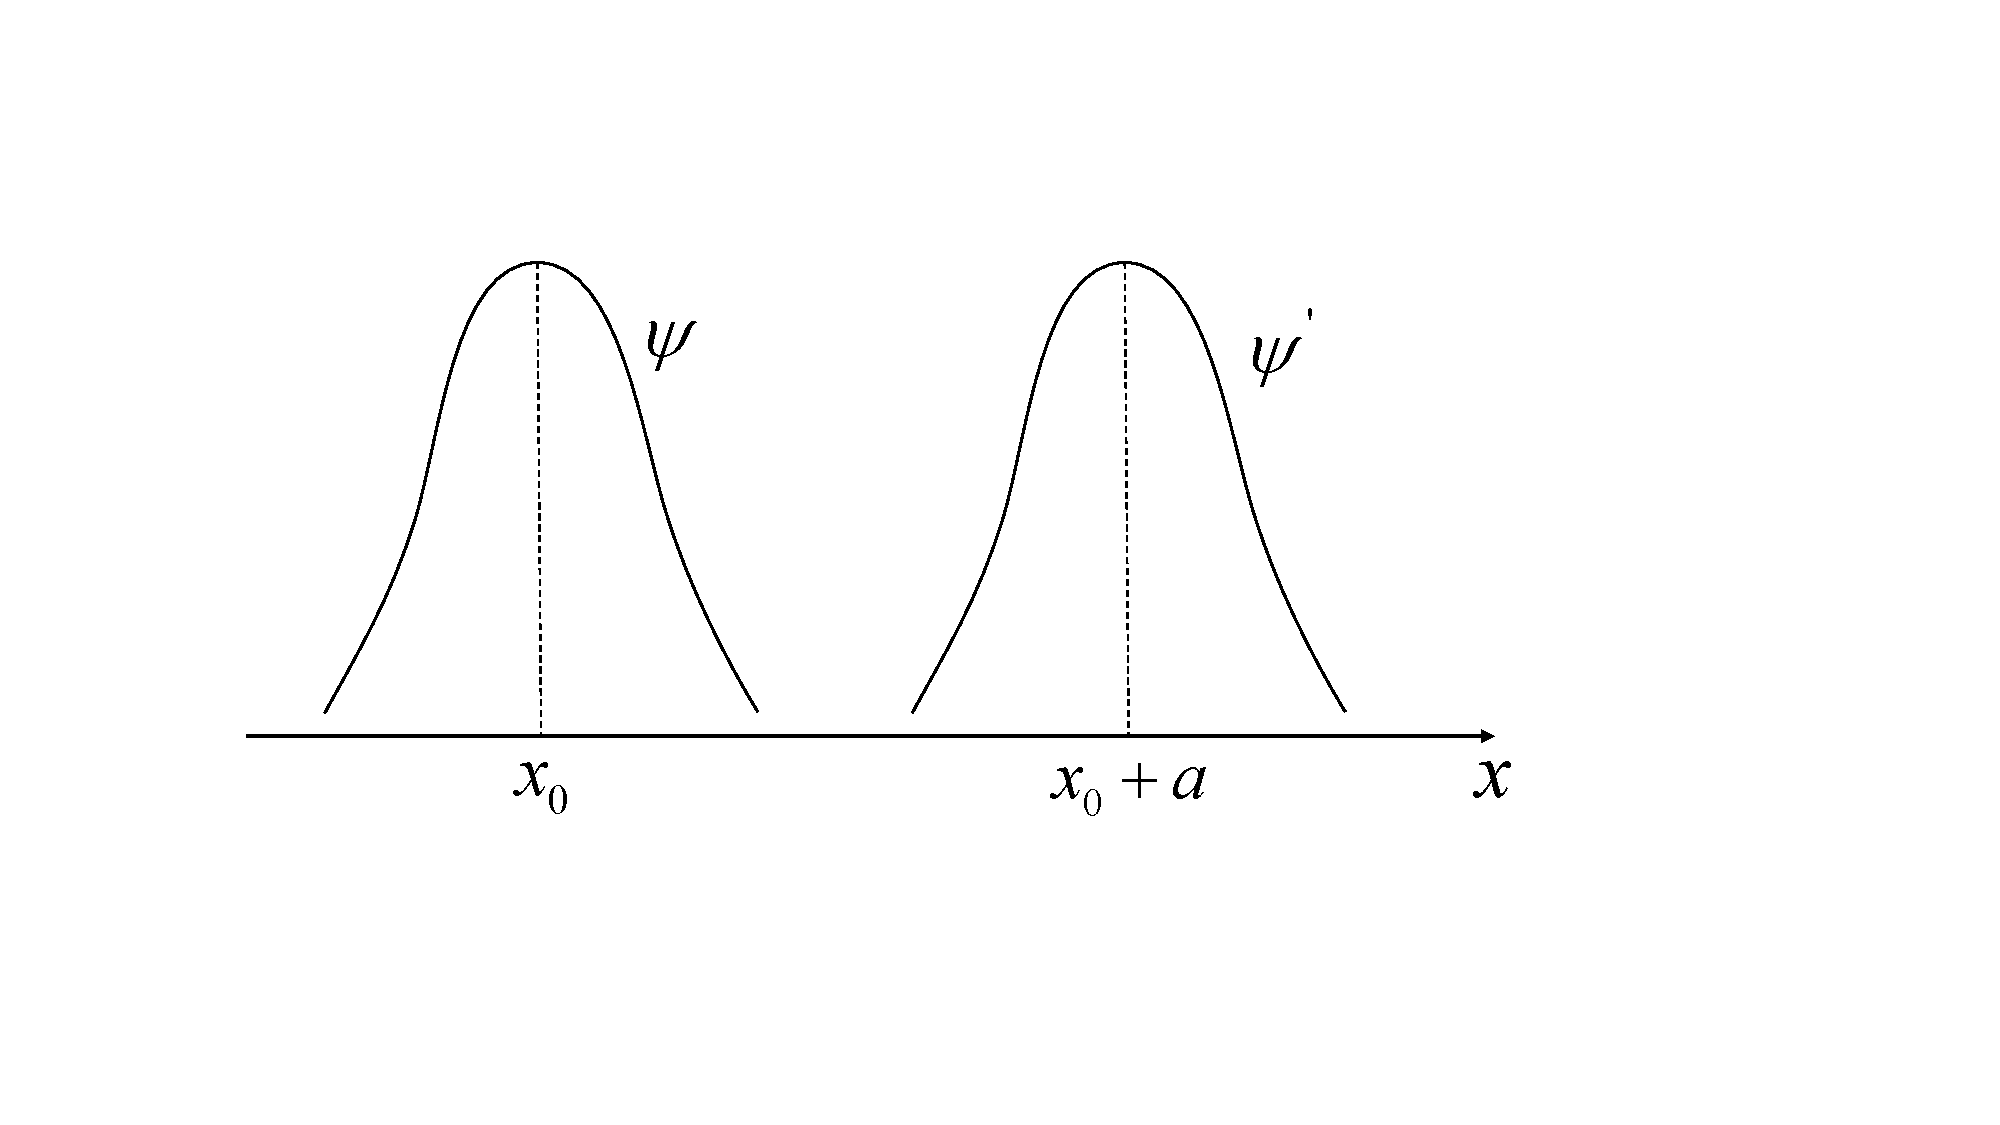
\includegraphics[width=3.5cm,clip]{QM file/figure/3-4}
	\caption{}\label{fig.3-4}
\end{wrapfigure}
\begin{empheq}{equation*}
	\varPsi^{\prime}(x)=\hat{D}(a)\varPsi(x)
\end{empheq}
显然
\begin{empheq}{equation*}
	\varPsi^{\prime}(x+a)=\varPsi(x)
\end{empheq}
因此
\begin{empheq}{equation}\label{eq310.11}
	\varPsi^{\prime}(x)=\hat{D}(a)\varPsi(x)=\varPsi(x-a)
\end{empheq}
这就是平移算符$\hat{D}(a)$对波函数的作用规则.平移显然是一种连续变换.我们先来确定无穷小平移$(a=\delta x\rightarrow 0)$算符$\hat{D}(\delta x)$)的具体形式.按照定义\eqref{eq310.11}式,应有
\eqindent{6}
\begin{empheq}{align*}
	\hat{D}(\delta x)\varPsi(x)&=\varPsi(x-\delta x)	\\
	&=\varPsi(x)-\frac{\partial \varPsi}{\partial x}\delta x=\bigg(1-\delta x\frac{\partial}{\partial x}\bigg)\varPsi(x)
\end{empheq}
所以
\begin{empheq}{align}\label{eq310.12}
	\hat{D}(\delta x)&=1-\delta x\frac{\partial}{\partial x}=1+\delta x\frac{\hat{p}_{x}}{i\hbar}	\nonumber\\
	&=\exp\bigg(\delta x\frac{\hat{p}_{x}}{i\hbar}\bigg)\quad(\delta x\rightarrow 0)
\end{empheq}
其中$\hat{p}_{x}$是动量算符.平移有限距离$a$时,算符$\hat{D}(a)$显然可以表示成
\begin{empheq}{equation}\label{eq310.13}
	\hat{D}(a)=\exp\bigg(-a\frac{\partial}{\partial x}\bigg)=\exp\bigg(a\hat{p}_{x}{i\hbar}\bigg)
\end{empheq}\eqnormal
将其代入\eqref{eq310.11}式,即得
\begin{empheq}{align*}
	\varPsi(x-a)=\exp\bigg(-a\frac{\partial}{\partial x}\bigg)\varPsi(x)	\\
	\sum_{n=0}^{\infty}\frac{(-a)^{n}}{n!}\bigg(\frac{\partial}{\partial x}\bigg)^{n}\varPsi(x)
\end{empheq}
这正是$\varPsi(x-a)$的泰勒(Taylor)展开式.

由以上分析,可知平移确是一种么正变换,满足
\eqindent{6}
\begin{equation}\label{eq310.14}
	\hat{D}^{+}(a)=\exp\bigg(\frac{ia}{\hbar}\hat{p}_{x}\bigg)=\hat{D}^{-1}(a)=\hat{D}(-a)
\end{equation}\eqnormal
其无穷小算子就是动量算符$\hat{p}_{x}$.

如体系的总能量算符$\hat{H}$具有平移不变性,满足
\begin{equation}\label{eq310.15}
	\hat{D}(a)\hat{H}=\hat{H}\hat{D}(a)
\end{equation}
则$\hat{H}$必与$\hat{p}_{x}$对易,即
\begin{empheq}{equation}\label{eq310.16}
	[\hat{p}_{x},\hat{H}]=\hat{p}_{x}\hat{H}-\hat{H}\hat{p}_{x}=0
\end{empheq}
$\hat{p}_{x}$为守恒量,这就是动量守恒定律.对于$\hat{H}$取
\begin{empheq}{equation*}
	\hat{H}=\hat{T}+\hat{V}=-\frac{\hbar^{2}}{2m}\frac{\partial^{2}}{\partial x^{2}}+V(x)
\end{empheq}
的情形,平移不变性要求$[V,p_{x}]$,则
\begin{empheq}{equation*}
	\frac{\partial V}{\partial x}=0,\quad V(x)=c\text{(常量)}
\end{empheq}
在这条件下,体系的动量守恒.经典力学也有同样的结论.

推广到三维问题,对于无限小平移$\delta r=(\delta x,\delta y,\delta z)$,相应的平移算符记为$\hat{D}(\delta \boldsymbol{r})$,应该有
\eqindent{6}
\begin{empheq}{align*}
	\hat{D}(\delta \boldsymbol{r})\varPsi(\boldsymbol{r})&=\varPsi(\boldsymbol{r}-\delta\boldsymbol{r})	\\
	&=\varPsi(\boldsymbol{r})-\bigg(\frac{\partial\varPsi}{\partial x}\delta x+\frac{\partial\varPsi}{\partial y}\delta y+\frac{\partial\varPsi}{\partial z}\delta z\bigg)	\\
	&=\varPsi(\boldsymbol{r})\sim\delta\boldsymbol{r}\cdot\nabla\varPsi
\end{empheq}
所以
\begin{empheq}{align}\label{eq310.17}
	\hat{D}(\delta \boldsymbol{r})&=1-\delta \boldsymbol{r}\cdot\nabla=\exp(-\delta \boldsymbol{r}\cdot\nabla)	\nonumber\\
	&=\exp\bigg(\delta \boldsymbol{r}\cdot\frac{\hat{\boldsymbol{p}}}{i\hbar}\bigg)(\delta \boldsymbol{r}\rightarrow 0)
\end{empheq}\eqnormal
其中$\hat{p}=-i\hbar\nabla$为动量算符.

平移有限距离$\boldsymbol{a}$时,算符$\hat{D}(\boldsymbol{a})$可以表示成
\begin{empheq}{equation}\label{eq310.18}
	\hat{D}(\boldsymbol{a})=\exp(-\boldsymbol{a}\cdot\nabla)=\exp\bigg(\boldsymbol{a}\cdot\frac{\hat{\boldsymbol{p}}}{i\hbar}\bigg)
\end{empheq}
如体系总能量算符$\hat{H}$具有平移不变性,满足
\begin{empheq}{equation}\label{eq310.19}
	\hat{D}(\boldsymbol{a})\hat{H}=\hat{H}\hat{D}(\boldsymbol{a})
\end{empheq}
则$\boldsymbol{a}\cdot\hat{\boldsymbol{p}}=a\hat{p}_{a}$必与$\hat{H}$对易,$\hat{p}_{a}$为守恒量.如上式对任意$\boldsymbol{a}$成立,则
\eqindent{6}
\begin{empheq}{equation}\label{eq310.20}
	[\hat{p}_{\alpha},\hat{H}]=\hat{p}_{\alpha}\hat{H}-\hat{H}\hat{p}_{\alpha}=0,\quad\alpha=x,y,z
\end{empheq}\eqnormal
$\boldsymbol{p}$为守恒量,这就是动量守恒定律.$\hat{H}$取\eqref{eq310.10}式时,平移不变性要求$[V,\hat{p}_{\alpha}]=0(\alpha=x,y,z)$,则
\begin{empheq}{equation*}
	\frac{\partial V}{\partial x},\frac{\partial V}{\partial y}=0,\frac{\partial V}{\partial z}=0,V(\boldsymbol{r})=c\text{(常量)}
\end{empheq}
在这条件下,体系的动量守恒.

{\heiti 3. 旋转不变性和角动量守恒定律}

考虑体系绕任意轴$\boldsymbol{e}_{n}$的旋转,对于无穷小旋转角$\delta\varphi$,相应的转动算符记为$\hat{R}(\delta\varphi)$,$\delta\varphi=\boldsymbol{e}_{n}\delta\varphi$.体系的任何一个状态$\varPsi$,经无限小转动后,变成$\varPsi^{\prime}$,即$\hat{R}(\delta\varphi)\varPsi$,它与$\varPsi$的关系可以仿照平移变换而确定.先考虑一种简单情形,即转轴为球坐标系极轴($z$轴)的情形.令$\hat{R}(\delta\varphi)\varPsi=\varPsi^{\prime}$,显然有
\eqindent{4}
\begin{empheq}{align*}
	\varPsi^{\prime}(r,\theta,\varphi)&=\hat{R}(\delta\varphi)\varPsi(r,\theta,\varphi)=\varPsi(r,\theta,\varphi-\delta\varphi)	\\
	&=\varPsi(r,\theta,\varphi)-\frac{\partial\varPsi}{\partial\varphi}\delta\varphi=\bigg(1-\delta\varphi\frac{\partial}{\partial\varphi}\bigg)\varPsi(r,\theta,\varphi)
\end{empheq}\eqnormal

\begin{wrapfigure}[14]{r}{5em}
	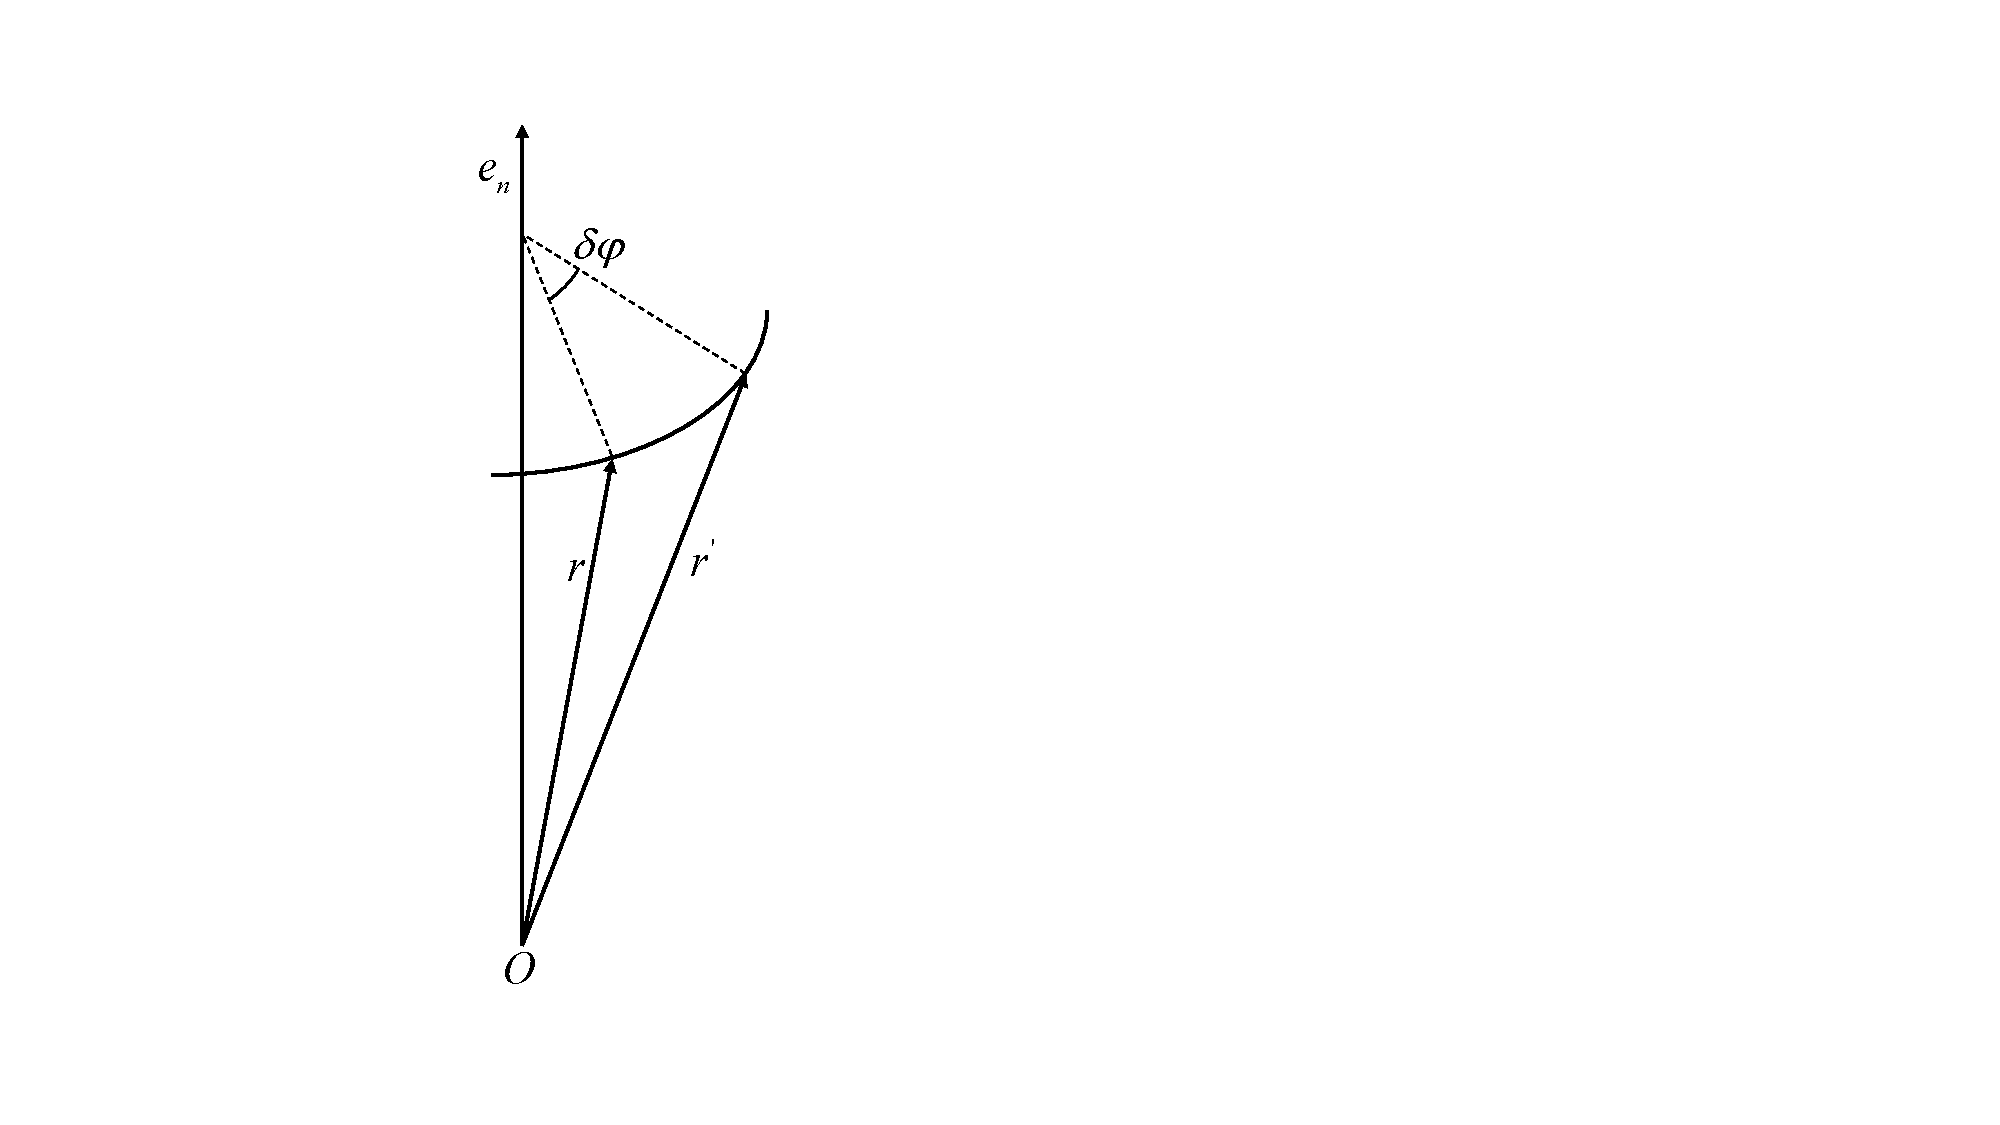
\includegraphics[width=2cm,clip]{QM file/figure/3-5}
	\caption{}\label{fig.3-5}
\end{wrapfigure}
所以
\eqindent{4}
\begin{empheq}{align}\label{eq310.21}
	\hat{R}(\delta\varphi)&=1-\delta\varphi\frac{\partial}{\partial\varphi}=1+\delta\varphi\frac{\hat{L}_{z}}{i\hbar}	\nonumber\\
	&=\exp\bigg(\delta\varphi\frac{\hat{L}_{z}}{i\hbar}\bigg)
\end{empheq}\eqnormal
其中
\eqindent{6}
\begin{empheq}{equation}\label{eq310.22}
	\hat{L}_{z}=-i\hbar\frac{\partial}{\partial\varphi}
\end{empheq}
为转动变换的无穷小算子,这就是轨道角动量($z$分量)算符.

当旋转轴$\boldsymbol{e}_{n}$沿任意方向时,矢径$\boldsymbol{r}$经过无穷小转动后变成(图\ref{fig.3-5})
\begin{empheq}{equation}\label{eq310.23}
	\boldsymbol{r}^{\prime}=\boldsymbol{r}+\delta\boldsymbol{r},\quad\delta\boldsymbol{r}=\delta\varphi\boldsymbol{e}_{n}\times\boldsymbol{r}
\end{empheq}
转动前后波函数关系为
\begin{empheq}{equation}\label{eq310.24}
	\varPsi^{\prime}(\boldsymbol{r}^{\prime})=\varPsi(\boldsymbol{r})
\end{empheq}
\begin{empheq}{align*}
	\varPsi^{\prime}(\boldsymbol{r})&=\hat{R}(\delta\varphi)\varPsi(\boldsymbol{r})=\varPsi(\boldsymbol{r}-\delta\boldsymbol{r})	\\
	&=\varPsi(\boldsymbol{r})-\delta\boldsymbol{r}\cdot\nabla\varPsi(\boldsymbol{r})=(1-\delta\boldsymbol{r}\cdot\nabla)\varPsi(\boldsymbol{r})	\\
	&=[1-\delta\varphi(\boldsymbol{e}_{n}\times\boldsymbol{r})\cdot\nabla]\varPsi(\boldsymbol{r})	\\
	&=[1-\delta\varphi\boldsymbol{e}_{n}\cdot(\boldsymbol{r}\times\nabla)]\varPsi(\boldsymbol{r})
\end{empheq}
所以
\begin{empheq}{align}\label{eq310.25}
	\hat{R}(\delta\varphi)&=1-\delta\varphi\boldsymbol{e}_{n}\cdot(\boldsymbol{r}\times\nabla)	\nonumber\\
	&=1+\frac{\delta\varphi}{i\hbar}\boldsymbol{e}_{n}\cdot\hat{\boldsymbol{L}}
	=\exp\bigg(\frac{\delta\varphi}{i\hbar}\boldsymbol{e}_{n}\cdot\hat{\boldsymbol{L}}\bigg)
\end{empheq}\eqnormal
其中
\begin{empheq}{equation}\label{eq310.26}
	\hat{\boldsymbol{L}}=-i\hbar\boldsymbol{r}\times\nabla=\boldsymbol{r}\times\hat{\boldsymbol{p}}
\end{empheq}
是轨道角动量算符,$\boldsymbol{e}_{n}\cdot\hat{\boldsymbol{L}}=\hat{L}_{n}$是转动变换的无穷小算子.

如体系具有对$\boldsymbol{e}_{n}$轴的旋转不变性,满足
\begin{empheq}{equation}\label{eq310.27}
	\hat{R}(\delta\varphi)\hat{H}=\hat{H}\hat{R}(\delta\varphi)
\end{empheq}
则$\hat{L}_{n}$与$\hat{H}$必然对易,即
\begin{empheq}{equation}\label{eq310.28}
	[\hat{L}_{n},\hat{H}]=\hat{L}_{n}\hat{H}-\hat{H}\hat{L}_{n}=0
\end{empheq}
$L_{n}$为守恒量.如$\hat{H}$具有对任意轴的旋转不变性,则$\hat{\boldsymbol{L}}$各分量均与$\hat{H}$对易,即
\begin{empheq}{equation}\label{eq310.29}
	[\hat{L}_{\alpha},\hat{H}]=\hat{L}_{\alpha}\hat{H}-\hat{H}\hat{L}_{\alpha}=0,\quad\alpha=x,y,z
\end{empheq}
$\boldsymbol{L}$为守恒量.在$\hat{H}$可以表示成\eqref{eq310.10}式的情形下,动能算符$\hat{T}=-\frac{\hbar^{2}}{2m}\nabla^{2}$具有对任意轴的旋转不变性,满足
\begin{empheq}{equation}\label{eq310.30}
	[\hat{L}_{\alpha},\hat{T}]=0,\quad\alpha=x,y,z
\end{empheq}
因此势能$V(r)$具有哪种旋转对称性,$\hat{H}$也具有同样的对称性.例如中心力场,$V=V(r)$,满足
\begin{empheq}{equation}\label{eq310.31}
	[\hat{L}_{\alpha},V(r)]=0,\quad\alpha=x,y,z
\end{empheq}
$V(r)$各向同性,具有对任意轴的旋转不变性,$\hat{H}$也一样,因此$\boldsymbol{L}$为守恒量,这就是角动量守恒定律.

{\heiti 4. 时间平移不变性和能量守恒定律}

在$\S$中\ref{sec:03.09}已经讲过,如体系的哈密顿算符$\hat{H}$不显含$t$,$\hat{H}$就是守恒量,这就是能量守恒定律.$\hat{H}$不显含$t$,意味着体系具有时间均匀性,体系能量不随时间变化,$\frac{\partial\hat{H}}{\partial t}$.当然,在量子力学中,时间$t$并不作为力学量对待,但是我们仍然可以仿照空间平移的概念,引入时间平移概念.任何状态$\varPsi(\boldsymbol{r},t)$的无穷小时间$(\delta t)$平移态记为$D_{t}(\delta t)\varPsi$,它在$t$时刻的情况与$\varPsi$态$(t+\delta t)$时刻的情况相同,即
\begin{empheq}{equation}\label{eq310.32}
	D_{t}(\delta t)\varPsi(\boldsymbol{r},t)=\varPsi(\boldsymbol{r},t+\delta t)
\end{empheq}
由于
\begin{empheq}{equation*}
	\varPsi(\boldsymbol{r},t+\delta t)=\varPsi(\boldsymbol{r},t)+\delta t\frac{\partial}{\partial t}\varPsi(\boldsymbol{r},t)
\end{empheq}
所以无穷小时间平移算符为
\begin{empheq}{equation}\label{eq310.33}
	D_{t}(\delta t)=1+\delta t\frac{\partial}{\partial t}=\exp\bigg(\delta t\frac{\partial}{\partial t}\bigg)
\end{empheq}
有限时间$(\tau)$平移算符为
\begin{empheq}{equation}\label{eq310.34}
	D_{t}(\tau)=\exp\bigg(\tau\frac{\partial}{\partial t}\bigg)
\end{empheq}
任何真实的运动状态$\varPsi(\boldsymbol{r},t)$应该满足薛定谔方程\eqref{eq310.1}式,$\frac{\partial}{\partial t}$对波函数的作用效果等价于$\frac{\hat{H}}{i\hbar}$,所以在时间平移算符中,可作如下等价代换:
\begin{empheq}{equation}\label{eq310.35}
	i\hbar\frac{\partial}{\partial t}\Longrightarrow\hat{H}
\end{empheq}
\begin{empheq}{equation}\label{eq310.36}
	D_{t}(\tau)\Longrightarrow\exp\bigg(\frac{\tau\hat{H}}{i\hbar}\bigg)
\end{empheq}
\eqref{eq310.35}式的含义正是$\S$\ref{sec:02.01}就已经讲过的,$i\hbar\frac{\partial}{\partial t}$代表能量.而\eqref{eq310.36}式表明,时间平移算符等价于演化算符[参看\eqref{eq39.7}式].

体系在时间上的均匀性也称时间平移不变性,这种对称性导致能量守恒定律成立.但应注意,这并不意味若体系在任何时刻必定处于能量本征态.这里“能量守恒”的确切内容是体系的能量平均值以及各个能量本征值的测量概率不随时间改变.以$\varPsi(\boldsymbol{r})$表示$\hat{H}$的本征态,本征值记为$E_{n}$.如在初始时刻$(t_{0}=0)$体系处于能量本征态$\varPsi_{n}$,波函数的时间演化规律为
\begin{empheq}{equation}\label{eq310.37}
	\varPsi_{n}(\boldsymbol{r},t)=\varPsi_{n}(\boldsymbol{r})e^{-E_{n}t/i\hbar}
\end{empheq}
这就是定态波函数.上式的时间平移$(\tau)$态为
\eqindent{6}
\begin{empheq}{align}\label{eq310.38}
	D_{t}\varPsi_{n}(\boldsymbol{r},t)&=e^{\tau\frac{\partial}{\partial t}}\varPsi_{n}(\boldsymbol{r})e^{-iE_{n}t/\hbar}	\nonumber\\
	&=\varPsi_{n}(\boldsymbol{r})\exp\bigg[-\frac{i}{\hbar}E_{n}(t+\tau)\bigg]
\end{empheq}\eqnormal
仍是原来的定态,只是添了相因子$\exp\bigg(-\frac{i}{\hbar}E_{n}(t+\tau)\bigg)$.如初始状态不是单一的能量本征态,则总可以表示成各$\varPsi_{n}$的线性叠加:
\begin{empheq}{equation}\label{eq310.39}
	\varPsi(\boldsymbol{r},t)=\sum_{n}C_{n}\varPsi_{n}(\boldsymbol{r})
\end{empheq}
波函数的时间演化规律为[\eqref{eq39.6}式]
\begin{empheq}{align}\label{eq310.40}
	\varPsi(\boldsymbol{r},0)&=\exp\bigg(\frac{\hat{H}t}{i\hbar}\bigg)\varPsi(\boldsymbol{r},0)	\nonumber\\
	&=\sum_{n}C_{n}\varPsi_{n}(\boldsymbol{r})e^{-E_{n}t/\hbar}
\end{empheq}
上式的时间平移$(\tau)$态为
\eqindent{6}
\begin{empheq}{align}\label{eq310.41}
	D_{t}(\tau)\varPsi(\boldsymbol{r},t)&=\exp\bigg(\frac{\hat{H}\tau}{i\hbar}\bigg)\varPsi(\boldsymbol{r},t)	\nonumber\\
	&=\exp\bigg[\frac{\hat{H}(t+\tau)}{i\hbar}\bigg]\varPsi(\boldsymbol{r},0)	\nonumber\\
	&=\sum_{n}C_{n}\varPsi_{n}(\boldsymbol{r})\exp\bigg[-\frac{i}{\hbar}E_{n}(t+\tau)\bigg]	\nonumber\\
	&=\varPsi(\boldsymbol{r},t+\tau)
\end{empheq}\eqnormal
显然,无论是\eqref{eq310.40}式还是\eqref{eq310.41}式,能量本征值$E_{n}$的测量概率均为$|C_{n}|^{2}$,与时间$t$及$\tau$无关,而仅取决于初始状态$\varPsi(\boldsymbol{r},0)$.

\example 质量为$m$的粒子作三维运动,已知总能量算符为
\begin{empheq}{equation}\label{eq310.42}
	\hat{H}=\hat{T}+V=-\frac{\hbar^{2}}{2m}\nabla^{2}+\frac{k}{2}(x^{2}+y^{2})
\end{empheq}
试分析其对称性并找出相应的守恒量.

\solution 首先,$\hat{H}$不显含$t$,具有时间均匀性,$H$为守恒量(能量守恒).$H_{x}=\frac{p_{x}^{2}}{2m}+\frac{kx^{2}}{2}$,$H_{y}=\frac{p_{y}^{2}}{2m}+\frac{ky^{2}}{2}$和$H_{z}=\frac{p_{z}^{2}}{2m}+\frac{kz^{2}}{2}$也都是守恒量.

其次,$\hat{H}$显然具有空间反射不变性,所以宇称守恒.

由于势能$V$与$z$无关,$\hat{H}$具有$z$方向平移不变性,所以动量的$z$分量$p_{z}$是守恒量.

势能$V$还具有绕$z$轴的旋转不变性,$\frac{\partial V}{\partial\varphi}$,所以轨道角动盘的$z$分量$L_{z}$,也是守恒量.








% 海尔曼定理和位力定理
\section[海尔曼定理和位力定理]{海尔曼定理和位力定理} \label{sec:03.11} % 
% \makebox[5em][s]{} % 短题目拉间距

关于物理体系的能量本征态(束缚态),有许多定理,其中最重要、应用最广的大概就是海尔曼(H.Hellmann)定理和位力(Virial) 定理了.海尔曼定理发表于20世纪30年代后期,最初是用来讨论量子化学问题的,因此在量子力学教科书中较少提到它.其实这个定理应用极广.
\newpage
{\heiti 1. 海尔曼定理}

设某个体系的束缚态能级和归一化能量本征函数为$E_{n}$,$\varPsi_{n}$($n$代表全体量子数或本征态编号数),满足能量本征方程
\begin{empheq}{equation}\label{eq311.1}
	\hat{H}\varPsi_{n}-E_{n}\varPsi_{n}=0
\end{empheq}
设$\lambda$为$\hat{H}$中含有的任何一个参数(如粒子质量$m$,普朗克常数$\hbar$,等等),显然$E_{n}$,$\varPsi_{n}$均与$\lambda$有关.\eqref{eq311.1}式对$\lambda$求导,得到
\begin{empheq}{equation*}
	\bigg(\frac{\partial\hat{H}}{\partial\lambda}-\frac{\partial E_{n}}{\partial \lambda}\bigg)\varPsi_{n}+(\hat{H}-E_{n})\frac{\partial\varPsi_{n}}{\partial\lambda}=0
\end{empheq}
左乘$\varPsi^{*}$,对全空间积分,得到
\eqindent{6}
\begin{empheq}{align}\label{eq311.2}
	\int\varPsi^{*}(\hat{H}-E_{n})\frac{\partial\varPsi_{n}}{\partial\lambda}d\tau
	&=\int\varPsi_{n}^{*}\bigg(\frac{\partial E_{n}}{\partial\lambda}-\frac{\partial\hat{H}}{\partial\lambda}\bigg)\varPsi_{n}d\tau	\nonumber\\
	&=\frac{\partial E_{n}}{\partial \lambda}-\bigg\langle\frac{\partial\hat{H}}{\partial\lambda}\bigg\rangle_{n}
\end{empheq}
其中$\langle\rangle_{n}$表示$\varPsi_{n}$态下的平均值.由于$\hat{H}=\hat{H}^{+}$,上式左端与$\hat{H}$有关的积分即
\begin{empheq}{align*}
	\int\varPsi^{*}\hat{H}\frac{\partial\varPsi_{n}}{\partial\lambda}d\tau
	&=\int\frac{\partial\varPsi_{n}}{\partial\lambda}(\hat{H}\varPsi_{n})^{*}d\tau	\\
	&=E_{n}\int\frac{\partial\varPsi_{n}}{\partial\lambda}\varPsi_{n}^{*}d\tau
\end{empheq}\eqnormal
因此\eqref{eq311.2}式左端等于0,于是得到
\begin{empheq}{equation}\label{eq311.3}
	\boxed{\frac{\partial E_{n}}{\partial\lambda}=\bigg\langle\frac{\partial\hat{H}}{\partial\lambda}\bigg\rangle_{n}\equiv\int\varPsi_{n}^{*}\frac{\partial\hat{H}}{\partial\lambda}\varPsi_{n}d\tau}
\end{empheq}
\eqref{eq311.3}式称为海尔曼定理或海尔曼公式.

适当地选择参数$\lambda$,$\frac{\partial\hat{H}}{\partial\lambda}$常常可以表示某些重要的力学量算符,所以利用海尔曼定理常可求出某些重要力学量的平均值,或求出能级.海尔曼定理也常用作理论分析的工具,例如用它来证明其他定理,下面先证明一个定理.

\theorem 粒子在势场$V_{1}(x)$中运动时,束缚态能级为$E_{n}(1)$;在势场$V_{2}(x)$中运动时,束缚态能级为$E_{n}(2)$.其中$n=1,2,3,\cdots$为能级编号.设对于任何$x$值,均有$V_{1}(x)\leqslant V_{2}(x)$,则
\begin{empheq}{equation*}
	E_{n}(1)\leqslant E_{n}(2)
\end{empheq}

\prove 考虑另一个介乎$V_{1},V_{2}$之间的势场
\eqindent{5}
\begin{empheq}{equation}\label{eq311.4}
	V(\lambda,x)=(2-\lambda)V_{1}(x)+(\lambda-1)V_{2}(x),\quad 1\leqslant \lambda\leqslant 2
\end{empheq}\eqnormal
当$\lambda=1,2,$上式即$V_{1}(x),V_{2}(x)$.粒子在势场$V(\lambda,x)$中运动时,总能量算符为
\begin{empheq}{equation}\label{eq311.5}
	\hat{H}(\lambda,x)=-\frac{\hbar^{2}}{2m}\frac{d^{2}}{dx^{2}}+V(\lambda,x)
\end{empheq}
相应的束缚态能级记为$E_{n}(\lambda)$,$n=1,2,3,\cdots$.\eqref{eq311.1}式对$\lambda$求导,得到
\begin{empheq}{equation*}
	\frac{\partial\hat{H}}{\partial\lambda}=\frac{\partial V(\lambda,x)}{\partial\lambda}=V_{2}(x)-V_{1}(x)\geqslant 0
\end{empheq}
由海尔曼定理,即得
\begin{empheq}{equation*}
	\frac{\partial}{\partial\lambda}E_{n}(\lambda)=\langle V_{2}-V_{1} \rangle_{n}\geqslant 0
\end{empheq}
这表明$\lambda$增加时$E_{n}(\lambda)$只增不减,所以$E_{n}(1)\geqslant E_{n}(2)$.

这个定理常用来对不同势场所造成的能级作定性比较分析.

\exa 已知一维谐振子的总能量算符和能级为
\begin{empheq}{equation}\label{eq311.6}
	\hat{H}=\hat{T}+V=-\frac{h^{2}}{2m}\frac{d^{2}}{dx^{2}}+\frac{1}{2}m\omega^{2}x^{2}
\end{empheq}
\begin{empheq}{equation}\label{eq311.7}
	E_{n}=\bigg(n+\frac{1}{2}\bigg)\hbar\omega,\quad n=0,1,2,\cdots
\end{empheq}

试用海尔曼定理证明,在能量本征态$\varPsi_{n}$下,
\begin{empheq}{equation}\label{eq311.8}
	\bar{T}=\bar{V}=\frac{1}{2}E_{n}
\end{empheq}

\prove 总能量算符$\hat{H}$中含有三个参数$\hbar$,$m$,$\omega$,其中任何一个均可取作海尔曼定理\eqref{eq311.3}式中的$\lambda$.如取$\lambda=\hbar$,
\begin{empheq}{equation*}
	\frac{\partial\hat{H}}{\partial\lambda}=-\frac{\hbar}{m}\frac{d^{2}}{dx^{2}}=\frac{2}{\hbar}\hat{T}
\end{empheq}
按照\eqref{eq311.3}式,就有
\begin{empheq}{equation*}
	\frac{\hbar}{\hbar}\langle T \rangle_{n}=\frac{\partial E_{n}}{\partial\hbar}=\bigg(n+\frac{1}{2}\bigg)\omega=\frac{E_{n}}{\hbar}
\end{empheq}
所以
\begin{empheq}{equation*}\label{eq311.8'}
	\langle T \rangle_{n}=\frac{1}{2}E_{n}	\tag{$3.11.8^{\prime}$}
\end{empheq}
由于
\begin{empheq}{equation*}
	E_{n}=\langle T+V \rangle_{n}
\end{empheq}
所以
\begin{empheq}{equation*}\label{eq311.8''}
	\langle V \rangle_{n}=E_{n}-\langle T \rangle_{n}=\frac{1}{2}E_{n}	\tag{$3.11.8^{\prime\prime}$}
\end{empheq}
如取$\lambda=m$或$\omega$,同样可以证明\eqref{eq311.8}式,读者试自完成之.

\exa 质量$m$,电荷$q$的粒子,受到弹性力$(-kx)$和均匀电场$\mathscr{E}$(指向正$x$轴方向)的共同作用,势能可以表示成
\begin{empheq}{equation}\label{eq311.9}
	V(x)=\frac{1}{2}kx^{2}-q\mathscr{E}x
\end{empheq}

求束缚能级.

\solution 总能量算符为
\begin{empheq}{equation}\label{eq311.10}
	\hat{H}=\hat{T}+V=-\frac{\hbar^{2}}{2m}\frac{d^{2}}{dx^{2}}+\frac{1}{2}kx^{2}-q\mathscr{E}x
\end{empheq}
视电场强度$\mathscr{E}$为参数,设能级为$E_{n}(\mathscr{E})$.当$\mathscr{E}=0$,\eqref{eq311.10}式即谐振子能量算符,其本征值为
\begin{empheq}{equation}\label{eq311.11}
	E_{n}(0)=\bigg(n+\frac{1}{2}\bigg)\hbar\omega,\quad\omega=\sqrt{\frac{k}{m}}
\end{empheq}
\eqref{eq311.10}式对$\mathscr{E}$求导,得到$\frac{\partial\hat{H}}{\partial\mathscr{E}}=-qx$,再利用海尔曼定理,即得
\begin{empheq}{equation}\label{eq311.12}
	\frac{\partial}{\partial\mathscr{E}}E_{n}(\mathscr{E})=-q\langle x \rangle_{n}
\end{empheq}
另一方面,
\begin{empheq}{align}\label{eq311.13}
	[\hat{p}_{x},\hat{H}]&=\frac{k}{2}[\hat{p}_{x},x^{2}]-q\mathscr{E}[\hat{p}_{x},x]	\nonumber\\
	&=-i\hbar(kx-q\mathscr{E})
\end{empheq}
上式在$\varPsi_{n}$态下求平均,由于
\begin{empheq}{equation*}
	[p_{x},H]=\int\varPsi_{n}^{*}(\hat{p}_{x}\hat{H}-\hat{H\hat{p}_{x}})\varPsi_{n}dx=0
\end{empheq}
(请读者自己证明)故得
\begin{empheq}{equation}\label{eq311.14}
	\langle x \rangle_{n}=\frac{q\mathscr{E}}{k}=\frac{q\mathscr{E}}{m\omega^{2}}
\end{empheq}
代入\eqref{eq311.12}式,得到
\begin{empheq}{equation*}\label{eq311.12'}
	\frac{\partial}{\partial\mathscr{E}}E_{n}(\mathscr{E})=-\frac{q^{2}\mathscr{E}}{k}	\tag{$3.11.12^{\prime}$}
\end{empheq}
积分,即得
\eqindent{5}
\begin{empheq}{gather}\label{eq311.15}
	E_{n}(\mathscr{E})=E_{n}(0)-\frac{q^{2}\mathscr{E}^{2}}{2k}=\bigg(n+\frac{1}{2}\bigg)\hbar\omega-\frac{q^{2}\mathscr{E}^{2}}{2m\omega^{2}}	\\ 
	\qquad \qquad \qquad n=0,1,2,\cdots	\nonumber
\end{empheq}\eqnormal
这就是所求束缚能级.请将本例和$\S$\ref{sec:02.05}的例题对照比较.
\newpage
{\heiti 2. 位力定理}

在经典力学中,质量为$m$的质点在势场$V(r)$中运动时,运动方程为
\begin{empheq}{equation}\label{eq311.16}
	\boldsymbol{p}=m\frac{d\boldsymbol{r}}{dt},\quad\frac{d\boldsymbol{p}}{dt}=\boldsymbol{F}=-\nabla V
\end{empheq}
因此
\eqindent{6}
\begin{empheq}{equation}\label{eq311.17}
	\frac{d}{dt}(\boldsymbol{r}\cdot\boldsymbol{p})=\frac{d\boldsymbol{r}}{dt}\cdot\boldsymbol{p}+\boldsymbol{r}\cdot\frac{d\boldsymbol{p}}{dt}=\frac{\boldsymbol{p}^{2}}{m}-\boldsymbol{r}\cdot\nabla V
\end{empheq}
如果粒子被局限在有限范图内运动(例如沿闭合轨道作周期运动),$\boldsymbol{r}\cdot\boldsymbol{p}$必取有限值,取\eqref{eq311.17}式的长时间平均(对于周期运动,取周期平均值),左端的平均必然等于0,故得
\begin{empheq}{equation}\label{eq311.18}
	\bigg(\frac{\boldsymbol{p}^{2}}{2m}\bigg)_{\text{平均}}=\frac{1}{2}(\boldsymbol{r}\cdot\nabla)_{\text{平均}}=-\frac{1}{2}(\boldsymbol{r}\cdot\boldsymbol{F})_{\text{平均}}
\end{empheq}
这就是经典力学中的位力定理.由于动能总是正的,所以$\boldsymbol{r}\cdot\boldsymbol{F}$的平均值应该是负的,亦即$\boldsymbol{F}$的性质是以吸引力为主.只有这样才能将粒子限制在有限区域内运动.

在量子力学中,当粒子在势场$V(\boldsymbol{r})$ 中运动时,总能量算符为
\begin{empheq}{equation}\label{eq311.19}
	\hat{H}=\hat{T}+\hat{V}=-\frac{\hbar^{2}}{2m}\nabla^{2}+V(\boldsymbol{r})
\end{empheq}
利用\eqref{eq39.17'},\eqref{eq39.18'},\eqref{eq39.32}式,可以证明算符公式
\begin{empheq}{equation}\label{eq311.20}
	\frac{d}{dt}(\hat{\boldsymbol{r}}\cdot\hat{\boldsymbol{p}})\equiv\frac{1}{i\hbar}[\hat{\boldsymbol{r}}\cdot\hat{\boldsymbol{p}},\hat{H}]=\frac{\hat{\boldsymbol{p}}^{2}}{m}-\boldsymbol{r}\cdot\nabla V
\end{empheq}
上式对任何一个能量本征态(束缚态)$\varPsi_{n}$取平均值,由于
\begin{empheq}{equation*}
	\langle[\hat{\boldsymbol{r}}\cdot\hat{\boldsymbol{p}},\hat{H}]\rangle_{n}
	\equiv\int\varPsi_{n}^{*}(\hat{\boldsymbol{r}}\cdot\hat{\boldsymbol{p}}\hat{H}-\hat{H}\hat{\boldsymbol{r}}\cdot\hat{\boldsymbol{p}})\varPsi_{n}d\tau=0
\end{empheq}\eqnormal
故得
\begin{empheq}{equation}\label{eq311.21}
	\boxed{\langle \frac{\boldsymbol{p}^{2}}{2m} \rangle_{n}=\frac{1}{2}\langle \boldsymbol{r}\cdot\nabla V \rangle_{n}}
\end{empheq}
这就是量子力学中的位力定理,它是经典位力定理的推广.注意\eqref{eq311.18}式的平均是对时间的平均,\eqref{eq311.21}式则是对束缚定态平均.

也可以利用海尔曼定理并结合坐标的尺度变换来证明位力定理,如下.\eqref{eq311.19}式对$\hbar$求导,得到
\begin{empheq}{equation}\label{eq311.22}
	\frac{\partial\hat{H}}{\partial\hbar}=-\frac{\hbar}{m}\nabla^{2}=\frac{2}{\hbar}\frac{\hat{\boldsymbol{p}^{2}}}{2m}
\end{empheq}
再利用海尔曼定理,即得
\begin{empheq}{equation}\label{eq311.23}
	\langle\frac{\hat{\boldsymbol{p}^{2}}}{2m}\rangle_{n}=\frac{\hbar}{2}\frac{\partial E_{n}}{\partial\hbar}
\end{empheq}
另一方面,如作坐标的尺度变换,令
\begin{empheq}{equation}\label{eq311.24}
	\boldsymbol{R}=\frac{\boldsymbol{r}}{\hbar}=(X,Y,Z)
\end{empheq}
则
\eqindent{6}
\begin{empheq}{align*}\label{eq311.19'}
	\hat{H}&=-\frac{1}{2m}\nabla_{R}^{2}+V(\hbar\boldsymbol{R})	\\
	&=-\frac{1}{2m}\bigg(\frac{\partial^{2}}{\partial X^{2}}+\frac{\partial^{2}}{\partial Y^{2}}+\frac{\partial^{2}}{\partial Z^{2}}\bigg)+V(\hbar\boldsymbol{R})
	\tag{$3.11.19^{\prime}$}
\end{empheq}\eqnormal
这时
\begin{empheq}{equation}\label{eq311.25}
	\frac{\partial\hat{H}}{\partial\hbar}=\frac{\partial V}{\partial\hbar}=\frac{\partial\boldsymbol{r}}{\partial\hbar}\cdot\nabla V=\frac{\boldsymbol{r}}{\hbar}\cdot\nabla V(\boldsymbol{r})
\end{empheq}
坐标变换对能级当然没有影响,因此,再利用海尔曼定理,得到
\begin{empheq}{equation}\label{eq311.26}
	\langle \boldsymbol{r}\cdot\nabla V(\boldsymbol{r}) \rangle_{n}=\hbar\frac{\partial E_{n}}{\partial\hbar}
\end{empheq}
比较\eqref{eq311.23}、\eqref{eq311.26}式,即得
\begin{empheq}{equation}\label{eq311.27}
	\langle \frac{\boldsymbol{p}^{2}}{2m} \rangle_{n}=\frac{1}{2}\langle \boldsymbol{r}\cdot\nabla V(\boldsymbol{r}) \rangle_{n}=\frac{\hbar}{2}\frac{\partial E_{n}}{\partial\hbar}
\end{empheq}
其中第一个等式就是位力定理.

位力定理可以推广到多粒子体系.以$x_{\alpha}$($\alpha=1,2,\cdots,3N$,$N$为粒子数)表示各粒子的位置,体系的总动能算符可以表示成
\begin{empheq}{equation}\label{eq311.28}
	\hat{T}=\sum_{\alpha}\frac{1}{2m}\hat{p}_{\alpha}=-\hbar^{2}\sum_{\alpha}\frac{1}{2m_{\alpha}}\bigg(\frac{\partial}{\partial x_{\alpha}}\bigg)^{2}
\end{empheq}
体系的总势能(包括外场作用势和粒子间相互作用势)表示成
\begin{empheq}{equation}\label{eq311.29}
	V=V(x_{1},x_{2},\cdots,x_{\alpha},\cdots,x_{3N})
\end{empheq}
体系的总能量算符为
\begin{empheq}{equation}\label{eq311.30}
	\hat{H}=\hat{T}+V
\end{empheq}
仿照上述步骤,仍有
\begin{empheq}{equation}\label{eq311.31}
	\frac{\partial\hat{H}}{\partial\hbar}=\frac{2}{\hbar}\hat{T}=-2\hbar\sum_{\alpha}\frac{1}{2m}\bigg(\frac{\partial}{\partial x_{\alpha}}\bigg)^{2}
\end{empheq}
作尺度变换
\eqindent{12}
\begin{empheq}{equation}\label{eq311.32}
	X_{\alpha}=\frac{x_{\alpha}}{\hbar}
\end{empheq}\eqnormal
后,则有
\eqindent{4}
\begin{empheq}{equation}\label{eq311.33}
	\frac{\partial\hat{H}}{\partial\hbar}=\frac{\partial V}{\partial\hbar}=\sum_{\alpha}\frac{\partial x_{\alpha}}{\partial\hbar}\frac{\partial V}{\partial x_{\alpha}}=\frac{1}{\hbar}\sum_{\alpha}x_{\alpha}\frac{\partial V}{\partial x_{\alpha}}
\end{empheq}
利用海尔曼定理,得到
\begin{empheq}{equation}\label{eq311.34}
	\langle T \rangle_{n}=\sum_{\alpha}\frac{1}{2m_{\alpha}}\langle p_{\alpha}^{2}\rangle_{n}=\frac{1}{2}\sum_{\alpha}\bigg\langle x_{\alpha}\frac{\partial V}{\partial x_{\alpha}}\bigg\rangle_{n}=\frac{\hbar}{2}\frac{\partial E_{n}}{\partial\hbar}
\end{empheq}\eqnormal
这就是多粒子体系的位力定理.

如果势能$V$是全体$x_{\alpha}$的$\nu$次齐次函数,即
\begin{empheq}{equation}\label{eq311.35}
	V(\lambda x_{1},\lambda x_{2},\cdots)=\lambda^{\nu}V(x_{1},x_{2},\cdots)
\end{empheq}
上式对$\lambda$求导,再取$\lambda=1$,得到
\eqindent{12}
\begin{empheq}{equation}\label{eq311.36}
	\sum_{\alpha}x_{\alpha}\frac{\partial V}{\partial x_{\alpha}}=\nu V
\end{empheq}
对于单粒子体系,就是
\begin{empheq}{equation*}\label{eq311.36'}
	\boldsymbol{r}\cdot\nabla V=\nu V	\tag{$3.11.36^{\prime}$}
\end{empheq}\eqnormal
将\eqref{eq311.36}式代入\eqref{eq311.34}式[\eqref{eq311.36'}式代入\eqref{eq311.27}式],得到
\begin{empheq}{equation}\label{eq311.37}
	\boxed{\langle T \rangle_{n}=\frac{\nu}{2}\langle V \rangle_{n}=\frac{\hbar}{2}\frac{\partial E_{n}}{\partial\hbar}}
\end{empheq}
例如谐振子,$V\propto x^{2}$(或$r^{2}$),相当于$\nu=2$,故有
\begin{empheq}{equation}\label{eq311.38}
	\langle T \rangle_{n}=\langle V \rangle_{n}=\frac{E_{n}}{2}\quad (E_{n}\propto\hbar)
\end{empheq}
又如受反平方吸引力作用的粒子,$V\propto\frac{1}{r}$,相当于$\nu=-1$,所以
\begin{empheq}{equation}\label{eq311.39}
	\langle T \rangle_{n}=-\frac{1}{2}\langle V \rangle_{n}=-E_{n}\quad (E_{n}\propto\hbar^{-2})
\end{empheq}
多电子原子或分子,粒子间作用势为库仑势,相当于$\nu=-1$的情形,所以体系总动能和总势能的束缚定态平均值仍保持\eqref{eq311.39}式的关系.

\exa 粒子在下列势场中运动,

\begin{empheq}{equation}\label{eq311.40}
	V(x)=\lim_{\nu\rightarrow\infty}V_{0}\bigg(\frac{x}{a}\bigg)^{2\nu},a,V_{0}>0
\end{empheq}

讨论势场的性质,并求$T,V$的定态平均值与能级的关系.

\solution 显然当$|x|>a$,$V=\infty$;当$|x|<a$,$V=O$.所以\eqref{eq311.40}式代表宽$2a$的无限深势阱.$V(x)$是$x$的$2\nu(\nu\rightarrow\infty)$次函数,按照\eqref{eq311.37}式,
\begin{empheq}{equation}\label{eq311.41}
	\langle V \rangle_{n}=\frac{1}{\nu}\langle T \rangle_{n}=0,\quad(\nu\rightarrow\infty)
\end{empheq}
因此
\begin{empheq}{equation}\label{eq311.42}
	\langle T \rangle_{n}=E_{n}-\langle V \rangle_{n}=E_{n}
\end{empheq}
请将本题结果和$\S$\ref{sec:02.04}(1.)的结果联系起来理解.









% 习题
\begin{exercises}

\exercise 粒子在一维无限深势阱[$\S$\ref{sec:02.04}(1.)]中运动,已知初始波函数,$\varPsi(x,0)=\frac{1}{\sqrt{2}}[\varPsi_{1}(x)+\varPsi_{2}(x)]$,求$\varPsi(x,t)$,$\bar{E}$,$\overline{E^{2}}$,$\bar{x}(t)$.

\exercise 粒子在一维无限深势阱($0<x<a$,见2-5题)中运动,初始波函数为$\varPsi(x,0)=cx(a-x)$,$c$为归一化常数,请确定$c$,并计算各能量本征值$(E_{n})$的测量概率以及$\bar{E}$,$\Delta E$.

\exercise 已知平面转子(见2-6题)初始波函数为$\varPsi(\varphi,0)=A\sin^{2}\varphi$,$A$为归一化常数,请确定$A$,并求$\varPsi(\varphi,t)$以及$\bar{E}$,$\Delta E$.

\exercise 粒子作一维自由运动,$-\infty<x<\infty$,已知初始波函数为$\varPsi(x,0)=A(\sin^{2}k_{0}x+\cos k_{0}x)$,求$\varPsi(x,t)$,动量$(p_{x})$及动能的取值及概率以及平均值.

\exercise 一维谐振子,初始波函数为$\varPsi(x,0)=\frac{\sqrt{3}}{2}\varPsi_{0}(x)+\frac{1}{2}\varPsi_{1}(x)$,求:$\varPsi(x,t)$,$\bar{E}(t)$,$\bar{x}(t)$,$\bar{p}_{x}(t)$.

\exercise 谐振子处于基态,求动量分布概率,并据此计算动能平均值以及$\Delta p$,与2-14题的结果比较.

\exercise 一维谐振子$\bigg(V=\frac{kx^{2}}{2}\bigg)$处于基态.如势场突然变成$V_{2}(x)=kx^{2}$,即弹性力增大一倍.求$V_{2}$场的能级以及粒子处于新势场中基态的概率.

\exercise 粒子处于一维无限深势阱$(|x|<a)$中的基态.如势阱突然扩展至$|x|<2a$,(阱宽加倍)设扩展时粒子的波函数不变.求扩展后粒子能量的可能测值以及粒子处于新势阱基态的概率.

\exercise 证明:对于任何一维束缚态,$\overline{xp_{x}}=\frac{i\hbar}{2}$,$\overline{p_{x}x}=-\frac{i\hbar}{2}$,并举一个实例验证之.

\exercise 粒子作一维运动,如归一化波函数$\varPsi(x)=u(x)e^{i\hbar x}$,$u(x)$及$k$均为实数,求动量平
均值.

\exercise 利用基本对易式$[x,p_{x}]=i\hbar$等,计算$[p_{x},L_{y}]$,$[p_{x},L_{z}]$,并写出另外几个下标轮换$(x\rightarrow y\rightarrow z\rightarrow x)$公式.

\exercise 证明算符关系:
\begin{empheq}{align*}
	\boldsymbol{r}\times\boldsymbol{L}+\boldsymbol{L}\times\boldsymbol{r}&=2i\hbar\boldsymbol{r}	\\
	\boldsymbol{p}\times\boldsymbol{L}+\boldsymbol{L}\times\boldsymbol{p}&=2i\hbar\boldsymbol{p}
\end{empheq}

\exercise 设线性算符$F$不是厄密的,即$F\neq F^{+}$.试证明$F$可以分解成$F=A+iB$,$A,B$均为厄密算符.求$A,B$.

\exercise 设$U$为么正算符,$(UU^{+}=U^{*}U=1)$证明$U$必可分解成$U=A+iB$,$A,B$为对易$(AB=BA)$厄密算符,而且$A^{2}+B^{2}=1$.进一步再证明$U$可以表示成$U=e^{iD}$的形式,$D$为厄密算符.
[提示:$A,B$的共同本符函数是完备系,本征值$a_{n},b_{n}$.满足关系$a_{n}^{2}+b_{n}^{2}=1$.]

\exercise 算符$A$(无量纲)的指数函数定义成
\begin{empheq}{equation*}
	e^{A}=\sum_{n=0}^{\infty}\frac{A^{n}}{n!}=1+A+\frac{A^{2}}{2!}+\cdots+\frac{A^{n}}{n!}+\cdots
\end{empheq}

(a) 如$A,B$对易,证明$e^{A}e^{B}=e^{A+B}$

(b) 如$A,B$不对易,令$[A,B]=AB-BA=C_{1},[A,C_{1}]=C_{2},\cdots,[A,C_{n}]=C_{n+1}$,证明公式
\begin{empheq}{equation*}
	e^{A}Be^{-A}=B+\sum_{n=1}^{\infty}\frac{C_{n}}{n!}
\end{empheq}

\exercise 设$p,q$为无量纲算符,$[q,p]=i$,$f(q)$是$q$的解析函数.(可展开为正幕级数)证明下列公式:

\begin{tabular}{ll}
	(a) $[q^{n},p]=inq^{n-1}$ & (b) $[f,p]=i\frac{df}{dq}$ \\ 
	(c) $[e^{i\lambda q},p]=-\lambda e^{-i\lambda q}$($\lambda$为参数) & (d) $[q,p^{n}]=inp^{n-1}$ \\
	(e)	$[q,e^{i\lambda q}]=-\lambda e^{i\lambda q}$ & \\
\end{tabular}

\exercise 设算符$A,B$不对易,$[A,B]=C$,而$C$与$A$及$B$均可对易,即$[C,A]=0,[C,B]=0$.计算$[A,B^{n}]$,$[A,e^{B}]$,$[A,f(B)]$,$f(B)$为$B$的解析函数(可展开为正幕级数).

\exercise 同上题,证明Glauber公式:
\begin{empheq}{equation*}
	e^{A+B}=e^{A}e^{B}e^{-\frac{C}{2}}=e^{B}e^{A}e^{\frac{C}{2}}
\end{empheq}

[提示: 令$f(\lambda)=e^{\lambda A}e^{\lambda B}$,$\lambda$为参数,证明
\begin{empheq}{equation*}
	\frac{df(\lambda)}{d\lambda}=f(\lambda)(A+B+\lambda C)
\end{empheq}
再对$\lambda$积分$\cdots\cdots$最后取$\lambda=1$.]

\exercise 设力学量算符$A$满足的最简单的代数方程式是
\begin{empheq}{equation*}
	f(A)=A^{n}+C_{n-1}A^{n-1}+\cdots+C_{1}A+C_{0}=0
\end{empheq}
各$C_{i}$为常数.试证明:$A$有$n$个本征值,它们都是方程$f(x)=0$的根.

\exercise 设力学量$k$的算符可以表示成两个不对易算符$L$及$M$之积,$K=LM$,而$L,M$的对易式为$[L,M]=1$.$K$的本征函数、本征值记为$\varPsi_{n}$,$\lambda_{n}(n=1,2,\cdots)$试证明:

\noindent 函数$L\varPsi_{n},M\varPsi_{n}$如存在,则它们也是$K$的本征函数,本征值分别为$(\lambda_{n}-1),(\lambda_{n}+1)$.

\exercise 求能使$x-p_{x}$不确定度关系下限成立$\bigg(\Delta x\Delta p_{x}=\frac{\hbar}{2}\bigg)$的一维波函数.

\exercise 证明:对于$H=\frac{\boldsymbol{p}^{2}}{2m}+V(\boldsymbol{r})$的情形,在任何束缚定态下,$\boldsymbol{p}$各分量的平均值为0.

\exercise 粒子在一维势场$V(x)=k|x|^{\nu}(k,\nu>0)$中运动,利用不确定度关系估算基态能级及$\Delta x$的量级.

\exercise 核子(质子,中子)间的核力(强作用)通过吞吐$\pi$介子而传递,$m_{\pi}\approx 270m_{e}$.试利用不确定度关系估算核力力程.

\exercise 质量$m$,电荷$q$的粒子在均匀电场(场强$\mathscr{E}$,沿正$x$轴方向)中运动,能量算符为$H=\frac{p_{x}^{2}}{2m}=-q\mathscr{E}x$.已知$t=0$时$\bar{x}=0,\bar{p}_{x}=p_{0}$,试利用海森堡方程计算$\bar{x}(t),\bar{p}_{x}(t)$.

\exercise 带电粒子在均匀磁场(沿$z$轴方向)中运动时,哈密顿算符可以近似表示成$H=\frac{\boldsymbol{p}^{2}}{2m}-\omega\boldsymbol{L}$,$\omega=\frac{qB}{2mc}$,$q$为粒子的电荷,$B$为场强.已知$t=0$时$\bar{p}_{x}=p_{0}$,$\bar{p}_{y}=\bar{p}_{z}$,试求$t>0$时$\bar{p}_{x}(t),\bar{p}_{y}(t),\bar{p}_{z}(t)$.又,本题有哪些重要的守恒力学量?

\exercise 对于一维谐振子,求海森堡图像中算符$\hat{x}(t)$,$\hat{p}_{x}(t)$,将它们用$\hat{x},\hat{p}_{x},t$表示出来.

\exercise 粒子在势场$V(\boldsymbol{r})$中运动,设$V$与粒子的质量无关.证明:如粒子的质量增大,则束缚态能级下降.

[提示:利用海尔曼定理.]

\exercise 质量为$m$的粒子在对数函数型中心力场$V(\boldsymbol{r})=V_{0}\ln\bigg(\frac{r}{r_{0}})$中运动,$V_{0},r_{0}>0$并与质量$m$无关.试利用海尔曼定理和位力定理,证明:(a) 各个束缚态的能量虽然不同,但动能平均值相同. (b) 如改变粒子的质量,任何两个能级的间距不受影响.

\exercise 粒子作一维运动,哈密顿算符为$H=\frac{p^{2}}{2m}+\frac{\lambda}{m}p+\frac{k}{2}x^{2}$($p$即$p_{x},\lambda,k>0$)求能谱.

[提示:利用海尔曼定理和谐振子的结果.]



\end{exercises}



% 第四章 表象理论
\chapter{表象理论}\label{chp:04}
% \makebox[5em][s]{} % 短题目拉间距

% 狄拉克符号
\section[狄拉克符号]{狄拉克符号} \label{sec:04.01} % 
% \makebox[5em][s]{} % 短题目拉间距

量子力学创始人之一狄拉克(P.A.M.Dirac)全面思考了量子力学的理论框架,综合考虑了复数、矢量代数、矩阵等数学领域的运算规则,创造性地发展了关于量子力学基本理论的整套概念与逻辑推理体系,制定了相应的数学符号与运算规则.狄拉克符号概念深刻,简洁方便,被国际物理学界广泛使用.

{\heiti 1.态矢空间}

按照狄拉克的观点,物理体系的每一个微观状态可以用一种抽象的多维矢量空间(Hilbert space)中的矢量来描述,这种矢量称为态矢,全体态矢构成态矢空间.提出这种观点的主要依据之一就是态叠加原理,其表述方式
\begin{empheq}{equation}\label{eq41.1}
	\varPsi=C_{1}\varPsi_{1}+C_{2}\varPsi_{2}+\cdots
\end{empheq}
与矢量间的线性叠加关系极其相似.

态矢空间包括右矢空间与共轭的左矢空间.右矢(ket)符号为$|\rangle$,左矢(bra)符号为$\langle|$.与$\varPsi$态对应的右矢记成$|\varPsi \rangle$,左矢记成$\langle \varPsi|$.共轭运算用符号$^{*}$表示.规定
\begin{empheq}{equation}\label{eq41.2}
	|\varPsi \rangle^{+}=\langle \varPsi|,\quad \varPsi\langle^{+} |=|\varPsi \rangle
\end{empheq}
数(实数或复数)$C$可以与右矢或左矢相乘,仍为右矢或左矢.规定这种乘法与次序无关,即规定
\begin{empheq}{equation}\label{eq41.3}
	C|\varPsi \rangle=\langle \varPsi|C,\quad C\langle \varPsi|=\langle \varPsi|C
\end{empheq}
数$C$的共轭规定成就是复共轭(符号$^{*}$),即
\begin{empheq}{equation}\label{eq41.4}
	C=\alpha+i\beta,\quad C^{+}=C^{*}=\alpha-i\beta
\end{empheq}
\eqindent{4}
\begin{empheq}{equation}\label{eq41.5}
	(C| \varPsi\rangle)^{*}=C^{*}\langle \varPsi|=\langle \varPsi|C^{*},\quad (C\langle \varPsi|)^{*}=C^{*}|\varPsi \rangle=|\varPsi \rangle C^{*}
\end{empheq}\eqnormal
这样,与态叠加原理\eqref{eq41.1}式对应的态右矢关系规定成
\begin{empheq}{equation}\label{eq41.6}
	|\varPsi \rangle =C_{1}|\varPsi_{1} \rangle +C_{2}|\varPsi_{2} \rangle +\cdots=\sum_{n}C_{n}|\varPsi_{n} \rangle 
\end{empheq}
对应的左矢关系则是
\begin{empheq}{equation*}\label{eq41.6'}
	\langle \varPsi|=C_{1}^{*}\langle \varPsi_{1}|+C_{2}^{*}\langle \varPsi_{2}|+\cdots=\sum_{n}\langle \varPsi_{n}|C_{n}^{*}	\tag{$4.1.6^{\prime}$}
\end{empheq}
左矢与右矢可以按“左矢在左、右矢在右”:即$\langle | | \rangle $的方式相乘,规定其性质是数,称为二态矢的“内积”.共轭运算规则为
\begin{empheq}{equation}\label{eq41.7}
	(\langle \varPsi|\phi \rangle )^{+}=\langle \phi|\varPsi \rangle =(\langle \varPsi|\phi \rangle )^{*}
\end{empheq}
其中$\langle \varPsi|\phi \rangle $是$\langle \varPsi||\phi \rangle $的简化写法.

如内积$\langle \varPsi|\phi \rangle=0$,称态矢$|\varPsi \rangle $,$|\phi \rangle $相互“正交”.任意态矢$|\varPsi \rangle $与自身的内积$\langle \varPsi|\varPsi \rangle $必为实数,规定其为正数,称为$|\varPsi \rangle $的“模方”,有时也记为$||\varPsi \rangle |^{2}$.注意
\begin{empheq}{equation}\label{eq41.8}
	|C|\varPsi \rangle |^{2}=\langle \varPsi|C^{*}C|\varPsi \rangle =C^{*}C\langle \varPsi|\varPsi \rangle 
\end{empheq}
如模方$\langle \varPsi|\varPsi \rangle$,称$|\varPsi \rangle $是归一化的.如$|\varPsi \rangle $并未归一化,只要$\langle \varPsi|\varPsi \rangle $有限,容易找到适当系数$C$,使$C|\varPsi \rangle $是归一化的.注意$C|\varPsi \rangle $与$|\varPsi \rangle $描述的是同一种状态.

态矢空间是希尔伯特(Hilbert)空间,原则上存在满足正交归一条件
\begin{empheq}{equation}\label{eq41.9}
	\langle \varPsi_{n}|\varPsi_{k} \rangle =\delta_{nk}
\end{empheq}
的基矢组$\{|\varPsi_{n} \rangle,n=1,2,\cdots \}$,基矢组具有完备性,任意态矢$|\varPsi \rangle $均可表示成基矢的线性叠加:
\begin{empheq}{equation*}
	|\varPsi \rangle =\sum_{n}C_{n}|\varPsi_{n} \rangle 
\end{empheq}
为了简化符号,基矢$|\varPsi_{n} \rangle $记成$|n \rangle $,上式写成
\begin{empheq}{equation}\label{eq41.10}
	|\varPsi \rangle =\sum_{n}C_{n}|n \rangle
\end{empheq}
基矢的正交归一条件\eqref{eq41.9}式即
\eqindent{12}
\begin{empheq}{equation*}\label{eq41.9'}
	\langle n|k \rangle =\delta_{nk}	\tag{$4.1.9^{\prime}$}
\end{empheq}\eqnormal
利用\eqref{eq41.9'}式,容易求出\eqref{eq41.10}式中各$C_{n}$为
\begin{empheq}{equation}\label{eq41.11}
	C_{n}=\langle n|\varPsi \rangle,\quad C_{n}^{+}=\langle \varPsi|n \rangle 
\end{empheq}
$|\varPsi \rangle $的模方为
\begin{empheq}{equation}\label{eq41.12}
	\langle \varPsi|\varPsi \rangle =\sum_{n}C_{n}^{*}C_{n}>0
\end{empheq}
考虑另一个态矢
\begin{empheq}{equation}\label{eq41.13}
	|\phi \rangle =\sum_{n}b_{n}|n \rangle ,\quad b_{n}=\langle n|\phi \rangle 
\end{empheq}
则$|\varPsi \rangle $,$|\phi \rangle $的内积为
\eqindent{6}
\begin{empheq}{equation*}
	\langle \varPsi|\phi \rangle =\sum_{n}C_{n}^{*}b_{n},\quad \langle \phi|\varPsi \rangle =\sum_{n}b_{n}^{*}C_{n}=(\langle \varPsi|\phi \rangle )^{*}
\end{empheq}\eqnormal

{\heiti 2.线性算符}

以$\hat{A},\hat{B},\hat{F},\hat{G}$等表示线性算符,规定它们可以作用于右矢及左矢,结果仍为右矢及左矢.允许的作用方式为
\eqindent{12}
\begin{empheq}{equation*}
	\hat{A}| \rangle \rightarrow | \rangle ,\quad \langle |\hat{B}\rightarrow \langle |
\end{empheq}\eqnormal
诸如$\hat{A}\langle |$,$| \rangle \hat{A}$等方式则是不允许的,没有意义.当态矢由\eqref{eq41.6}、\eqref{eq41.6'}表示时,线性算符$\hat{A}$的作用规则是
\begin{empheq}{equation}\label{eq41.14}
	\hat{A}\bigg(\sum_{n}C_{n}|\varPsi_{n} \rangle \bigg)=\sum_{n}C_{n}\hat{A}|\varPsi_{n} \rangle 
\end{empheq}
\begin{empheq}{equation*}\label{eq41.14'}
	\bigg(\sum_{n}\langle \varPsi_{n}|C_{n}^{*} \bigg)\hat{A}=\sum_{n}C_{n}\langle \varPsi_{n}|\hat{A}	\tag{$4.1.14^{\prime}$}
\end{empheq}
原则上,定义一个线性算符$\hat{A}$,需要规定$\hat{A}$对全部基矢的作用结果,即规定$\hat{A}|n \rangle $,$\langle n|\hat{A}$,$n=1,2,\cdots$.等价地,相当于规定全部$\langle k|\hat{A}|n \rangle $.习惯上常用符号
\eqindent{12}
\begin{empheq}{equation}\label{eq41.15}
	\langle k|\hat{A}|n \rangle\equiv A_{kn}
\end{empheq}\eqnormal
注意其性质是“数”.上式常称为算符$\hat{A}$的“矩阵元”,这名称的来由参看\eqref{eq41.17}式以下的说明以及$\S$\ref{sec:04.02}.

算符$\hat{A}$的共轭算符记为$\hat{A}^{*}$,按下式定义:
\eqindent{7}
\begin{empheq}{equation}\label{eq41.16}
	(\hat{A}|\varPsi \rangle )^{*}=\langle \varPsi|\hat{A}^{+},\quad (\langle \varPsi|\hat{A})^{+}=\hat{A}^{+}|\varPsi \rangle 
\end{empheq}
$|\varPsi \rangle $为任意态矢.将上式用于基矢,就有
\begin{empheq}{equation}\label{eq41.17}
	(A_{kn})^{*}=(\langle k|\hat{A}|n \rangle )^{+}=\langle n|\hat{A}^{+}|k \rangle =A_{nk}^{+}
\end{empheq}\eqnormal
也可以将\eqref{eq41.17}式作为$\hat{A}^{+}$的定义.如将各$\hat{A}_{kn}$按行列次序排成矩阵($k$代表行,$n$代表列),各$\hat{A}_{nk}^{+}$也排成矩阵,二者刚好互为共轭矩阵.

如果对于各基矢$|n \rangle $,$|k \rangle $,均有$A_{kn}^{*}$,则必有$\hat{A}=\hat{A}^{+}$.反之亦然.具有这种性质的算符,称为厄密(Hermite) 算符.

如态矢$|\varPsi \rangle $与线性算符$\hat{F}$满足关系(本征方程)
\begin{empheq}{equation}\label{eq41.18}
	\hat{F}|\varPsi \rangle =\lambda|\varPsi \rangle ,\quad \lambda\text{为数}
\end{empheq}
则称$|\varPsi \rangle $为$\hat{F}$的本征矢,$\lambda$为$\hat{F}$的本征值.上式的共轭方程是
\begin{empheq}{equation*}\label{eq41.18'}
	\langle \varPsi|\hat{F}^{+}=\lambda^{*}\langle \varPsi|
\end{empheq}
如果$\hat{F}\neq\hat{F}^{+}$,本征值一般为复数.可以证明,如$\hat{F}$是厄密算符$(\hat{F}=\hat{F}^{+})$,则本征值必为实数.以定理的形式证明如下.

\theo 厄密算符的本征值必为实数.

\prove 设$\hat{F}\neq\hat{F}^{+}$,以$\langle \varPsi|$乘本征方程\eqref{eq41.18},就有
\begin{empheq}{equation*}
	\langle \varPsi|\hat{F}|\varPsi \rangle =\lambda\langle \varPsi|\varPsi \rangle 
\end{empheq}
上式两端均取共轭,由于$\hat{F}\neq\hat{F}^{+}$,就有
\begin{empheq}{equation*}
	(\langle \varPsi|\hat{F}|\varPsi \rangle )^{+}=\langle \varPsi|\hat{F}|\varPsi \rangle =\lambda^{*}\langle \varPsi|\varPsi \rangle 
\end{empheq}
二式左端相同,右端由于$\langle \varPsi|\varPsi \rangle\neq 0$,故有$\lambda=\lambda^{*}$,$\lambda$为实数.

关于厄密算符,还有本征矢的正交定理,如下.

\theo 如$|\varPsi_{1} \rangle$,$|\varPsi_{2} \rangle$是厄密算符$\hat{F}$的两个本征矢,相应于不同的本征值,则$|\varPsi_{1} \rangle$,$|\varPsi_{2} \rangle$正交.

\prove $|\varPsi_{1} \rangle$,$|\varPsi_{2} \rangle$分别满足本征方程
\begin{empheq}{equation}\label{eq41.19}
	\hat{F}|\varPsi_{1} \rangle =\lambda_{1}|\varPsi_{1} \rangle ,\quad \hat{F}|\varPsi_{2} \rangle =\lambda_{2}|\varPsi_{2} \rangle 
\end{empheq}
它们的共轭方程是(注意$\hat{F}=\hat{F}^{+}$,$\lambda_{1},\lambda_{2}$是实数)
\begin{empheq}{equation*}\label{eq41.19'}
	\langle \varPsi_{1}|\hat{F}=\lambda_{1}\langle \varPsi_{1}|,\quad \langle \varPsi_{2}|\hat{F}=\lambda_{2}\langle \varPsi_{2}|	\tag{$4.1.19^{\prime}$}
\end{empheq}
以$\langle \varPsi_{2}|$乘\eqref{eq41.19}第一式,得到
\eqindent{12}
\begin{empheq}{equation*}
	\langle \varPsi_{2}|\hat{F}|\varPsi_{1} \rangle =\lambda_{1}\langle \varPsi_{2}|\varPsi_{1} \rangle 
\end{empheq}
\eqref{eq41.19'}式乘$|\varPsi_{1} \rangle $,则得
\begin{empheq}{equation*}
	\langle \varPsi_{2}|\hat{F}|\varPsi_{1} \rangle =\lambda_{2}\langle \varPsi_{2}|\varPsi_{1} \rangle 
\end{empheq}\eqnormal
二式左端相同,右端由于$\lambda_{1}\neq\lambda_{2}$,必然有$\langle \varPsi_{2}|\varPsi_{1} \rangle=0$.

两个线性算符$\hat{A},\hat{B}$之和记为$(\hat{A}+\hat{B})$,对态矢的作用规则为
\begin{empheq}{equation}\label{eq41.20}
	(\hat{A}+\hat{B})|\varPsi \rangle = \hat{A}|\varPsi \rangle +\hat{B}|\varPsi \rangle 
\end{empheq}
显然$(\hat{A}+\hat{B})=(\hat{B}+\hat{A})$.$\hat{A},\hat{B}$之积记为$(\hat{A}\hat{B})$或$\hat{B}\hat{A}$,对态矢的作用规则为
\eqindent{6}
\begin{empheq}{equation}\label{eq41.21}
	(\hat{A}\hat{B})|\varPsi \rangle =\hat{A}(\hat{B}|\varPsi \rangle ),\quad \langle \varPsi|(\hat{A}\hat{B})=(\langle \varPsi|\hat{A}) \hat{B}
\end{empheq}
一般说,$\hat{A}\hat{B}\neq\hat{B}\hat{A}$.如果$\hat{A}\hat{B}=\hat{B}\hat{A}$,称$\hat{A},\hat{B}$对易.由\eqref{eq41.20}、\eqref{eq41.21}式,再利用\eqref{eq41.16}式,容易证明
\begin{empheq}{equation}\label{eq41.22}
	(\hat{A}+\hat{B})^{+}=\hat{A}^{+}+\hat{B}^{+},\quad (\hat{A}\hat{B})^{+}=\hat{B}^{+}\hat{A}^{+}
\end{empheq}\eqnormal
这样,如$\hat{A},\hat{B}$均为厄密算符,则$(\hat{A}+\hat{B})$也是厄密算符.如$\hat{A},\hat{B}$为互相对易的厄密算符,则$(\hat{A}\hat{B})$也是厄密算符.

前面讲过,构造式$\langle | \rangle $即$\langle || \rangle $的性质是“数”.那么构造$|\rangle \langle| $式的性质又是什么?易见任何左矢$\langle \varPsi|$从左与它相乘,结果仍为左矢;它与右矢$|\varPsi \rangle $相乘($|\varPsi \rangle $在右),结果仍为右矢.所以$|\rangle \langle|$的性质是线性算符.例如,将\eqref{eq41.11}式代入\eqref{eq41.10}式,可得
\begin{empheq}{equation*}
	|\varPsi \rangle =\sum_{n}|n \rangle C_{n}=\sum_{n}|n \rangle\langle n|\varPsi \rangle  
\end{empheq}
因为$|\varPsi \rangle $可以是任何态矢,故知
\eqindent{12}
\begin{empheq}{equation}\label{eq41.23}
	\boxed{\sum_{n}|n \rangle\langle n|=1}
\end{empheq}\eqnormal
称为恒等变换算符.在涉及表象变换的计算中,\eqref{eq41.23}式极其有用.读者应该熟记此式,在需要用它的场合能及时想到.

\example 给定一个归一化的态矢$|\phi \rangle$,并定义“投影算符”
\begin{empheq}{equation}\label{eq41.24}
	\hat{P}_{\phi}=|\phi \rangle\langle \phi|
\end{empheq}
求$\hat{P}_{\phi}$的本征值、本征矢.研究$\hat{P}_{\phi}$作用于任意态矢$|\varPsi \rangle $将得到什么结果.

\solution 显然$\hat{P}_{\phi}$是厄密算符,其本征值应该是实数.另外,
\begin{empheq}{equation*}
	\hat{P}_{\phi}^{2}=|\phi \rangle\langle \phi||\phi \rangle\langle \phi|=|\phi \rangle\langle \phi|=\hat{P}_{\phi}
\end{empheq}
即
\begin{empheq}{equation}\label{eq41.25}
	\hat{P}_{\phi}^{2}-\hat{P}_{\phi}=\hat{P}_{\phi}(\hat{P}_{\phi}-1)=0
\end{empheq}
设$\hat{P}_{\phi}$的本征值为$\lambda$,本征矢为$|\varPsi_{\lambda} \rangle $,满足本征方程
\begin{empheq}{equation}\label{eq41.26}
	\hat{P}_{\phi}|\varPsi_{\lambda} \rangle =\lambda|\varPsi_{\lambda} \rangle 
\end{empheq}
将\eqref{eq41.25}式作用于$|\varPsi_{\lambda} \rangle $,得到
\begin{empheq}{equation}\label{eq41.27}
	\lambda(\lambda-1)=0,\quad \lambda=1,0
\end{empheq}
将$\lambda=1$代入\eqref{eq41.26}式,得到
\begin{empheq}{equation*}
	\hat{P}_{\phi}|\varPsi_{1} \rangle=|\phi \rangle\langle \phi|\varPsi_{1} \rangle=|\varPsi \rangle 
\end{empheq}
可见$|\varPsi_{1} \rangle=C|\phi \rangle $,系数$C$并无实质性意义,可取为1,亦即相应于本征值$\lambda=1$的$\hat{P}_{\phi}$本征矢就是$|\phi \rangle $.

将$\lambda=0$代入\eqref{eq41.26}式,得到
\begin{empheq}{equation*}
	\hat{P}_{\phi}|\varPsi_{0} \rangle=|\phi \rangle\langle \phi|\varPsi_{0} \rangle=0,\quad \langle \phi|\varPsi_{0} \rangle=0
\end{empheq}
可知一切与$|\phi \rangle $正交的态矢$|\varPsi_{0} \rangle $都是$\hat{P}_{\phi}$的本征矢,相应本征值$\lambda=0$.

$\hat{P}_{\phi}$作用于任意态矢$|\varPsi \rangle $,结果为
\eqindent{6}
\begin{empheq}{equation}\label{eq41.28}
	\hat{P}_{\phi}|\varPsi \rangle=|\phi \rangle\langle \phi|\varPsi \rangle=C_{\phi}|\phi \rangle,\quad C_{\phi}=\langle \phi|\varPsi \rangle 
\end{empheq}\eqnormal
可见,$\hat{P}_{\phi}$的作用是将$|\varPsi \rangle $转变成$C_{\phi}|\phi \rangle $,换言之,将态矢$|\varPsi \rangle $向$|\phi \rangle $“方向”投影.
















% 量子力学公式及其矩阵表示
\section[量子力学公式及其矩阵表示]{量子力学公式及其矩阵表示} \label{sec:04.02} % 
% \makebox[5em][s]{} % 短题目拉间距

代表力学量(可观测量)的算符,如$\S$\ref{sec:03.04}所述,必须是厄密算符,其本征矢有正交归一性和完备性,因此可以选作态矢空间的基矢组.

选定一个力学量完全集$Q$,代表它的厄密算符记为$\hat{Q}$,其本征值记为$q_{n}$,本征矢记为$|\varPsi_{n} \rangle $,简记为$|n \rangle $,满足本征方程
\begin{empheq}{equation}\label{eq42.1}
	\hat{Q}|n \rangle=q_{n}|n \rangle ,\quad \langle n|\hat{Q}=q_{n}\langle n|
\end{empheq}
正交归一条件
\begin{empheq}{equation}\label{eq42.2}
	\langle \varPsi_{n}|\varPsi_{k} \rangle=\langle n|k \rangle =\delta_{nk}
\end{empheq}
以及综合了本征矢的正交归一性与完备性的恒等变换公式
\begin{empheq}{equation}\label{eq42.3}
	\sum_{n}|\varPsi_{n} \rangle\langle \varPsi_{n}|=\sum_{n}|n \rangle\langle n|=1  
\end{empheq}
以$\{|n \rangle,n=1,2,\cdots\}$作为基矢组,任何态矢$|\varPsi \rangle $可以表示成
\eqindent{4}
\begin{empheq}{equation}\label{eq42.4}
	|\varPsi \rangle =\sum_{n}|n \rangle\langle n|\varPsi \rangle =\sum_{n}C_{n}|n \rangle,\quad
	C_{n}\langle n|\varPsi \rangle 
\end{empheq}\eqnormal
如$|\varPsi \rangle $已经归一化,$\langle \varPsi|\varPsi \rangle=1$,就有
\begin{empheq}{equation}\label{eq42.5}
	\langle \varPsi|\varPsi \rangle =\sum_{n}C_{n}^{*}C_{n}=1
\end{empheq}
其中
\eqindent{6}
\begin{empheq}{equation}\label{eq42.6}
	C_{n}^{*}C_{n}=\text{在$|\varPsi\rangle$态中力学量$Q$取值为$q_{n}$的概率}
\end{empheq}\eqnormal
这正是态矢$|\varPsi \rangle $的概率解释.力学量$Q$的平均值公式可以表示成
\begin{empheq}{align}\label{eq42.7}
	\bar{Q}&=\sum_{n}q_{n}C_{n}C_{n}^{*}=\sum_{n}q_{n}C_{n}\langle \varPsi|n \rangle	\nonumber\\
	&=\langle \varPsi|\sum_{n}C_{n}\hat{Q}|n \rangle =\langle \varPsi|\hat{Q}\sum_{n}C_{n}|n \rangle 	\nonumber\\
	&= \langle \varPsi|\hat{Q}|n \rangle 
\end{empheq}
如利用基矢$|n \rangle $的投影算符
\begin{empheq}{equation}\label{eq42.8}
	\hat{P}_{n}=|n \rangle\langle n|
\end{empheq}
\eqref{eq42.6}式中概率$C_{n}^{*}C_{n}$可以表示成
\eqindent{6}
\begin{empheq}{equation}\label{eq42.9}
	C_{n}^{*}C_{n}=\langle \varPsi|n \rangle \langle n|\varPsi \rangle =\langle \varPsi|\hat{P}_{n}|\varPsi \rangle =\bar{P}_{n}
\end{empheq}
这是投影算符的又一层含义.

在$|\varPsi \rangle $的展开式\eqref{eq42.4}中,如将各$C_{n}$排成一个列矢量(单列矩阵),记为$\varPsi(Q)$,即定义
\begin{empheq}{equation}\label{eq42.10}
	\varPsi(Q)=\begin{bmatrix}
		C_{1}\\ \vdots\\ C_{n}\\ \vdots
	\end{bmatrix}
	,\quad
	\varPsi^{*}(Q)=\begin{bmatrix}
		C_{1}^{*} & \cdots & C_{n}^{*} & \cdots
	\end{bmatrix}
\end{empheq}
$\varPsi^{*}(Q)$是$\varPsi(Q)$的共轭矩阵,是一个行矢量.按照矩阵运算法则,
\begin{empheq}{equation}\label{eq42.11}
	\varPsi^{+}(Q)\varPsi(Q)=\begin{bmatrix}
		\cdots & C_{n}^{*} & \cdots
	\end{bmatrix}	\begin{bmatrix}
		\vdots \\ C_{n} \\ \vdots
	\end{bmatrix}
\end{empheq}
$\varPsi(Q)$作为列矢量,称为态矢$|\varPsi\rangle$在$Q$表象中的矩阵表示.$\varPsi^{*}(Q)$作为行矢量,则为$\langle \varPsi|$在$Q$表象中的矩阵表示.

$\varPsi(Q)$也可以称为$|\varPsi\rangle$在$Q$表象中的“波函数”($\hat{Q}$的本征值的函数),其中$C_{n}=\varPsi(q_{n})$.

各基矢$|n \rangle $是$\hat{Q}$的本征矢,它们在$Q$表象中的矩阵表示(波函数)显然应该是
\begin{empheq}{equation}\label{eq42.12}
	\varPsi_{1}(Q)=\begin{bmatrix}
		1 \\ 0 \\ 0 \\ \vdots
	\end{bmatrix},\cdots,\quad
	\varPsi_{n}(Q)=\begin{bmatrix}
		\vdots \\ 0 \\ 1 \\ 0 \\ \vdots
	\end{bmatrix}\cdots
	\text{第$n$行}	
\end{empheq}
展开式\eqref{eq42.4}的矩阵表示为
\begin{empheq}{equation*}
	\varPsi(Q)=\begin{bmatrix}
		C_{1}\\ \vdots\\ C_{n}\\ \vdots
	\end{bmatrix}=C_{1}\varPsi_{1}(Q)+\cdots+C_{n}\varPsi_{n}(Q)+\cdots
\end{empheq}\eqnormal
相当于第三章讲过的波函数按本征函数的展开式.

{\heiti 线性算符的矩阵表示}

设有任意线性算符$\hat{A}$作用于任意态矢$|\varPsi \rangle $,将其转变成$|\phi \rangle $,即设
\begin{empheq}{equation}\label{eq42.13}
	\hat{A}|\varPsi \rangle =|\phi \rangle 
\end{empheq}
$|\varPsi\rangle$及其$Q$表象中的波函数$\varPsi(Q)$由\eqref{eq42.4}、\eqref{eq42.10}式表示.类似地,$|\phi \rangle $及其波函数$\phi(Q)$表示成
\eqindent{6}
\begin{empheq}{equation}\label{eq42.14}
	|\phi \rangle =\sum_{n}b_{n}|n \rangle ,\quad \phi(Q)=\begin{bmatrix}
		b_{1} \\ \vdots \\ b_{n} \\ \vdots
	\end{bmatrix},\quad
	b_{n=\langle n|\phi \rangle }
\end{empheq}
$Q$表象中算符$\hat{A}$的矩阵表示记为$[A]$,它应该可以与列矢量和行矢量相乘,而有
\begin{empheq}{equation*}
	[A]\begin{bmatrix}
		\cdot \\ \cdot \\ \cdot \\ \cdot
	\end{bmatrix}\rightarrow\begin{bmatrix}
		\cdot \\ \cdot \\ \cdot \\ \cdot
	\end{bmatrix},\quad
	\begin{bmatrix}
		\cdot & \cdot & \cdot & \cdot & \cdot
	\end{bmatrix}[A]\rightarrow\begin{bmatrix}
		\cdot & \cdot & \cdot & \cdot & \cdot
	\end{bmatrix}
\end{empheq}
具体说,与\eqref{eq42.13}式相应,$[A]$,$\varPsi(Q)$,$\phi(Q)$间应该有关系
\begin{empheq}{equation}\label{eq42.15}
	[A]\varPsi(Q)=[A]\begin{bmatrix}
		C_{1}\\ \vdots\\ C_{n}\\ \vdots
	\end{bmatrix}=\begin{bmatrix}
		b_{1}\\ \vdots\\ b_{n}\\ \vdots
	\end{bmatrix}=\phi(Q)
\end{empheq}\eqnormal
易见,符合上述要求的$[A]$应该是行、列数相同的矩阵,即方阵.$[A]$的$k$行$n$列矩阵元记为$A_{kn}$,可以证明
\begin{empheq}{equation}\label{eq42.16}
	A_{kn}=\langle k|\hat{A}|n \rangle 
\end{empheq}
证明如下.\eqref{eq42.15}式中列矢量$\phi(Q)$的第$k$个矩阵元是
\begin{empheq}{equation}\label{eq42.17}
	b_{k}=\sum_{n}A_{kn}C_{n}
\end{empheq}
另一方面,以基左矢$\langle k|$乘\eqref{eq42.13}式,得到
\begin{empheq}{align*}
	\langle k|\phi \rangle &=b_{k}=\langle k|\hat{A}|\varPsi \rangle =\sum_{n}\langle k|\hat{A}|n \rangle \langle n|\varPsi \rangle 	\\
	&=\sum_{n}\langle k|\hat{A}|n \rangle C_{n}
\end{empheq}
比较二式,即得\eqref{eq42.16}式.

\eqref{eq42.13}式的共轭方程是
\begin{empheq}{equation*}\label{eq42.13'}
	\langle \varPsi|\hat{A}^{+}=\langle \phi|	\tag{$4.2.13^{\prime}$}
\end{empheq}
其矩阵表示应该就是\eqref{eq42.15}式的共轭方程,即
\eqindent{3}
\begin{empheq}{equation*}\label{eq42.15'}
	\varPsi^{+}(Q)[A^{+}]=[C_{1}^{*}\cdots C_{n}^{*}\cdots][A^{+}]=
	[b_{1}^{*}\cdots b_{n}^{*}\cdots]=\phi^{*}(Q)
	\tag{$4.2.15^{\prime}$}
\end{empheq}\eqnormal
则
\begin{empheq}{equation*}
	b_{k}^{*}=\sum_{n}C_{n}^{+}A_{nk}^{+}
\end{empheq}
与\eqref{eq42.17}式的复共轭$(^{*})$比较,即得
\begin{empheq}{equation}\label{eq42.18}
	A_{nk}^{+}=(A_{kn})^{*}
\end{empheq}
这正是共轭矩阵的定义.

如$\hat{F}$是厄密算符,$\hat{F}=\hat{F}^{+}$,则在$Q$表象中其矩阵表示应该是厄密矩阵,即$[F]=[F]^{+},F_{nk}=(F_{kn})^{*}$.

$Q$表象中$\hat{Q}$本身的矩阵元是
\begin{empheq}{equation}\label{eq42.19}
	Q_{kn}=\langle k|\hat{Q}|n \rangle =q_{n}\langle k|n \rangle =q_{n}\delta_{kn}
\end{empheq}
矩阵$[Q]$是对角化方阵,对角矩阵元等于$\hat{Q}$的各本征值,非对角矩阵元全部为零,即
\eqindent{6}
\begin{empheq}{equation*}\label{eq42.19'}
	[Q]=\begin{bmatrix}
		q_{1} & 0 & 0 & \cdots & 0 & \cdots	\\
		0 & q_{2} & 0 & \cdots & 0 & \cdots	\\
		0 & 0 & q_{3} & \cdots & 0 & \cdots	\\
		\vdots & \vdots & \vdots & \quad & \vdots & 	\\
		0 & 0 & 0 & \cdots & q_{n} & \cdots	\\
		\vdots & \vdots & \vdots & \quad & \vdots & 	\\
	\end{bmatrix}	\tag{$4.2.19^{\prime}$}
\end{empheq}\eqnormal

{\heiti 平均值公式及其矩阵表示}

平均值公式\eqref{eq42.7}显然适用于任何可观测量$F$.即,对于任何归一化的状态$\varPsi$,$F$的平均值为
\begin{empheq}{equation}\label{eq42.20}
	\bar{F}=\langle \varPsi|\hat{F}|\varPsi \rangle 
\end{empheq}
利用\eqref{eq42.3}、\eqref{eq42.4}式及\eqref{eq42.10}、\eqref{eq42.16}式,可将上式化成矩阵形式,如下:
\eqindent{6}
\begin{empheq}{align}\label{eq42.21}
	\bar{F}&=\langle \varPsi|\hat{F}|\varPsi \rangle =\sum_{n}\sum_{k}C_{n}^{*}\langle n|\hat{F}|k \rangle C_{k}	\nonumber\\
	&=\sum_{n}\sum_{k}C_{n}^{*}F_{nk}C_{k}=[C_{1}^{*}\cdots C_{n}^{*}\cdots][F]\begin{bmatrix}
		C_{1} \\ \vdots \\ C_{n} \vdots
	\end{bmatrix}	\nonumber\\ &=\varPsi^{+}(Q)[F]\varPsi(Q)
\end{empheq}\eqnormal
这就是$\bar{F}$在$Q$表象中的矩阵表示式.从\eqref{eq42.20}式$\rightarrow$\eqref{eq42.7}式,相当于
\begin{empheq}{equation*}
	\langle \varPsi|\rightarrow \varPsi^{+}(Q),\quad |\varPsi \rangle \rightarrow \varPsi(Q),\quad \hat{F}\rightarrow [F]
\end{empheq}
\newpage
{\heiti 本征方程的矩阵表示}

求解力学量算符本征方程
\begin{empheq}{equation}\label{eq42.22}
	\hat{F}|\varPsi_{\lambda} \rangle =\lambda|\varPsi_{\lambda} \rangle 
\end{empheq}
的问题,也可以在$Q$表象中用矩阵方法来解决.$|\varPsi_{\lambda} \rangle $仍表示成\eqref{eq42.4}式,波函数$\varPsi_{\lambda}(Q)$仍由\eqref{eq42.10}式表示,各$C_{n}$待定.\eqref{eq42.22}式的矩阵表示为
\begin{empheq}{equation}\label{eq42.23}
	[F]\varPsi_{\lambda}(Q)=\lambda\varPsi_{\lambda}(Q)
\end{empheq}
亦即
\eqindent{6}
\begin{empheq}{equation*}\label{eq42.23'}
	\begin{bmatrix}
		F_{11}-\lambda & F_{12} & \cdots & F_{1n} & \cdots	\\
		F_{21} & F_{22}-\lambda & \cdots & F_{2n} & \cdots	\\
		\vdots & \vdots &  & \vdots & 	\\
		F_{n1}-\lambda & F_{n2} & \cdots & F_{nn}-\lambda & \cdots	\\
		\vdots & \vdots &  & \vdots & 	\\
	\end{bmatrix}\begin{bmatrix}
		C_{1} \\ C_{2} \\ \vdots \\ C_{n} \\ \vdots
	\end{bmatrix}=0	\tag{$4.2.23^{\prime}$}
\end{empheq}\eqnormal
这就是本征方程\eqref{eq42.22}式的矩阵表示.其中$[F]$的矩阵元均在$Q$表象中定义,$F_{kn}=\langle k|\hat{F}|n \rangle$.只要先求出$Q$表象中$\hat{F}$的矩阵表示,即求出各$F_{kn}$,由\eqref{eq42.23'}式即可解出本征值$\lambda$及各$C_{n}$,亦即解出$\lambda$及$\varPsi_{\lambda}(Q)$.具体说,\eqref{eq42.23'}式存在非平庸解(各$C_{n}$不全为零)的充要条件为
\eqindent{0}
\begin{empheq}{equation}\label{eq42.24}
	\det(F-\lambda I)=0,\text{即}\begin{bmatrix}
		F_{11}-\lambda & F_{12} & \cdots & F_{1n} & \cdots	\\
		F_{21} & F_{22}-\lambda & \cdots & F_{2n} & \cdots	\\
		\vdots & \vdots &  & \vdots & 	\\
		F_{n1}-\lambda & F_{n2} & \cdots & F_{nn}-\lambda & \cdots	\\
		\vdots & \vdots &  & \vdots & 	\\
	\end{bmatrix}=0
\end{empheq}\eqnormal
由此解出$\lambda=\lambda_{1},\lambda_{2},\cdots$将每个$\lambda$值代回\eqref{eq42.23'}式,求出相应的$C_{n}(n=1,2,\cdots)$,再代回\eqref{eq42.10}式,就得本征函数$\varPsi_{\lambda}(Q)$.

{\heiti 表象变换}

态矢空间的基矢组可以有多种选择.如另选一个力学量完全集$\boldsymbol{R}$,代表它的厄密算符记为$\hat{R}$,其正交归一的本征矢记为
\begin{empheq}{equation*}
	|\phi_{\nu} \rangle,\text{简记为}|\nu \rangle,\quad \nu=1,2,\cdots,\mu,\cdots
\end{empheq}
满足
\begin{empheq}{equation}\label{eq42.25}
	\langle \phi_{\nu}|\phi_{\mu} \rangle=\langle \nu|\mu \rangle =\delta_{\nu\mu}
\end{empheq}
\begin{empheq}{equation}\label{eq42.26}
	\sum_{\nu}|\phi_{\nu} \rangle\langle \phi_{\nu}|=\sum_{\nu}|\nu \rangle\langle \nu|=1 
\end{empheq}
以$\{|\phi_{\nu} \rangle \}$作为基矢组,任意态矢$|\varPsi \rangle $可以表示成
\begin{empheq}{equation}\label{eq42.27}
	|\varPsi \rangle=\sum_{\nu}a_{\nu}|\phi_{\nu} \rangle,\quad a_{\nu}=\langle \phi_{\nu}|\varPsi \rangle 
\end{empheq}
由各$a_{\nu}$组成的列矢量就是$|\varPsi \rangle $在$R$表象中的波函数:
\begin{empheq}{equation}\label{eq42.28}
	\varPsi(R)=\begin{bmatrix}
		a_{1} \\ \vdots \\ a_{\nu} \\ \vdots
	\end{bmatrix},\quad \varPsi^{+}(R)=[a_{1}^{*}\cdots a_{\nu}^{*}\cdots]
\end{empheq}
任意线性算符$\hat{A}$在$R$表象中的矩阵表示记为$A(R)$,其矩阵元为
\begin{empheq}{equation}\label{eq42.29}
	A_{\mu\nu}=\langle \phi_{\mu}|\hat{A}|\phi_{\nu} \rangle=\langle \mu|\hat{A}|\nu \rangle 
\end{empheq}
前述$Q$表象中$|\varPsi \rangle $的波函数符号仍用$\varPsi(Q)$,见\eqref{eq42.10}式.$Q$表象中$\hat{A}$的矩阵表示现在改记为$A(Q)$,其矩阵元由\eqref{eq42.16}式表示:
\begin{empheq}{equation*}
	A_{kn}=\langle \varPsi_{k}|\hat{A}|\varPsi_{n} \rangle =\langle k|\hat{A}|\nu \rangle 
	\tag{$4.2.16$}
\end{empheq}
试问,同一个态矢$|\varPsi \rangle $在两种表象中的矩阵表示即波函数$\varPsi(Q)$、$\varPsi(R)$之间有什么关系?同一个算符$\hat{A}$在两种表象中的矩阵表示$A(Q)$、$A(R)$之间又有什么关系?不妨设想$\varPsi(Q)$、$\varPsi(R)$可以用一个变换矩阵$S$联系起来:
\begin{empheq}{equation}\label{eq42.30}
	\varPsi(R)=S\varPsi(Q)
\end{empheq}
亦即
\eqindent{6}
\begin{empheq}{equation*}\label{eq42.30'}
	\begin{bmatrix}
		a_{1} \\ \vdots \\ a_{\nu} \\ \vdots
	\end{bmatrix}=[S]\begin{bmatrix}
		C_{1} \\ \vdots \\ C_{n} \\ \vdots
	\end{bmatrix}=\begin{bmatrix}
		S_{11} & \cdots & S_{1n} & \cdots	\\
		\vdots &  & \vdots & 	\\
		S_{\nu 1} & \cdots & S_{\nu n} & \cdots	\\
		\vdots &  & \vdots & 	\\
	\end{bmatrix}\begin{bmatrix}
		C_{1} \\ \vdots \\ C_{n} \\ \vdots
	\end{bmatrix}	\tag{$4.2.30^{\prime}$}
\end{empheq}\eqnormal
则
\begin{empheq}{equation*}
	a_{\nu}=\sum_{n}S_{\nu n}C_{n},\quad \text{即}\langle \phi_{\nu}|\varPsi \rangle =
	\sum_{n}S_{\nu n}\langle \varPsi_{n}|\varPsi \rangle 
\end{empheq}
利用恒等变换\eqref{eq42.3}式,有
\begin{empheq}{equation*}
	\langle \phi_{\nu}|=\sum_{n}\langle \phi_{\nu}|\varPsi_{n} \rangle \langle \varPsi_{n}|
\end{empheq}
代入上式, 即得
\begin{empheq}{equation}\label{eq42.31}
	S_{\nu n}=\langle \phi_{\nu}|\varPsi_{n} \rangle 
\end{empheq}
注意变换矩阵$S$完全由基矢组$\{|\varPsi_{n} \rangle\}$,$\{|\phi_{\nu} \rangle \}$的相互关系(具体说,就是内积)决定,而与$|\varPsi \rangle $无关.$S$的共轭矩阵记为$S^{+}$,其矩阵元为
\begin{empheq}{equation*}\label{eq42.31'}
	S_{n\nu}^{+}=(S_{\nu n})^{*}=\langle \varPsi_{n}|\phi_{\nu} \rangle 
	\tag{$4.2.31^{\prime}$}
\end{empheq}
$S^{+}S$和$SS^{+}$仍为矩阵,其矩阵元为
\eqindent{6}
\begin{empheq}{align}\label{eq42.32}
	\begin{aligned}
		[S^{+}S]_{nk} &=\sum_{\nu}S_{n\nu}^{+}S_{\nu k}=\sum_{\nu}\langle \varPsi_{n}|\phi_{\nu} \rangle\langle \phi_{\nu}|\varPsi_{k} \rangle  \\
		&=\langle \varPsi_{n}|\varPsi_{k} \rangle =\delta_{nk}
	\end{aligned}
	\\
	\begin{aligned} \notag
		[SS^{+}]_{\nu\mu} &=\sum_{n}S_{\nu n}S_{n\mu}^{+}=\sum_{n}\langle \phi_{\nu}|\varPsi_{n} \rangle\langle \varPsi_{n}|\phi_{\mu} \rangle  \\
		&=\langle \phi_{\nu}|\phi_{\mu} \rangle =\delta_{\nu\mu}
	\end{aligned}
\end{empheq}
可见$S^{+}S$和$SS^{+}$都是单位矩阵:
\begin{empheq}{equation}\label{eq42.33}
	S^{+}S=SS^{+}=\begin{bmatrix}
		1 & 0 & \cdots & 0	\\
		0 & 1 & \cdots & 0	\\
		\vdots & \vdots &  & \vdots	\\
		0 & 0 & \cdots & 1	\\
	\end{bmatrix}\Rightarrow 1
\end{empheq}\eqnormal
$S$与$S^{+}$因此称为么正矩阵.利用\eqref{eq42.33}式,容易得到\eqref{eq42.30}式的逆变换为
\begin{empheq}{equation}\label{eq42.34}
	\varPsi(Q)=S^{+}\varPsi(R)
\end{empheq}
$\varPsi^{*}(Q)$、$\varPsi^{*}(R)$的变换关系则是
\begin{empheq}{equation}\label{eq42.35}
	\varPsi^{+}(R)=\varPsi^{+}(Q)S^{+},\quad \varPsi^{+}(Q)=\varPsi^{+}(R)S
\end{empheq}
再看$A(Q)$、$A(R)$之间的关系.利用恒等变换\eqref{eq42.3}式,可得
\eqindent{4}
\begin{empheq}{align}\label{eq42.36}
	A_{\mu\nu}&=\langle \phi_{\mu}|\hat{A}|\phi_{\nu} \rangle=\sum_{n}\sum_{k}\langle \phi_{\mu}|\varPsi_{n} \rangle \langle \varPsi_{n}|\hat{A}|\varPsi_{k} \rangle \langle \varPsi_{k}|\phi_{\nu} \rangle 	\nonumber\\
	&=\sum_{n}\sum_{k}S_{\nu n}A_{nk}S_{k\nu}^{+}
\end{empheq}\eqnormal
按照矩阵乘法,上式相当于
\begin{empheq}{equation}\label{eq42.37}
	A(R)=SA(Q)S^{+}
\end{empheq}
逆变换为
\begin{empheq}{equation}\label{eq42.38}
	A(Q)=S^{+}A(R)S
\end{empheq}
表象变换时,态矢和算符的具体矩阵表示与所选表象有关,但它们所描述的物理内容则不受表象选择的影响.例举如下.

(1) 态矢的模方不变.态矢间内积不变.以模方为例,\eqref{eq42.11}式已证
\begin{empheq}{equation*}
	\langle \varPsi|\varPsi \rangle =\varPsi^{+}(Q)\varPsi(Q)
\end{empheq}
利用\eqref{eq42.33}、\eqref{eq42.34}、\eqref{eq42.35}式,即得
\begin{empheq}{align}\label{eq42.39}
	\langle \varPsi|\varPsi \rangle &=\varPsi^{+}(Q)\varPsi(Q)=\varPsi^{+}(R)SS^{+}\varPsi(R)	\nonumber\\
	&=\varPsi^{+}(R)\varPsi(R)
\end{empheq}
同样可证
\begin{empheq}{equation}\label{eq42.40}
	\langle \varPsi|\phi \rangle =\varPsi^{+}(Q)\phi(Q)=\varPsi^{+}(R)\phi(R)
\end{empheq}

(2) 力学量算符的本征值与表象选择无关.在$Q$表象中,$\hat{F}$的本征方程由\eqref{eq42.23}式表示,即
\begin{empheq}{equation*}
	F(Q)\varPsi_{\lambda}(Q)=\lambda\varPsi_{\lambda}(Q)
	\tag{$4.2.23$}
\end{empheq}
利用\eqref{eq42.33}、\eqref{eq42.34}、\eqref{eq42.38}式,上式成为
\begin{empheq}{equation*}
	S^{+}F(R)SS^{+}\varPsi_{\lambda}(R)=\lambda S^{+}\varPsi_{\lambda}(R)
\end{empheq}
用$S$乘上式,并利用\eqref{eq42.33}式,就有
\begin{empheq}{equation}\label{eq42.41}
	F(R)\varPsi_{\lambda}(R)=\lambda\varPsi_{\lambda}(R)
\end{empheq}
这正是$R$表象中$\hat{F}$的本征方程.注意由\eqref{eq42.23}式导出\eqref{eq42.41}式的过程中,本征值$\lambda$保持不变.

(3) 平均值公式不变前面\eqref{eq42.21}式已经证明
\begin{empheq}{equation}\label{eq42.42}
	\bar{F}=\langle \varPsi|\hat{F}|\varPsi \rangle =\varPsi^{+}(Q)F(Q)\varPsi(Q)
\end{empheq}
再用\eqref{eq42.33}、\eqref{eq42.34}、\eqref{eq42.35}、\eqref{eq42.38}式,就有
\eqindent{5}
\begin{empheq}{equation}\label{eq42.43}
	\bar{F}=\varPsi^{+}(R)SS^{+}F(R)SS^{+}\varPsi(R)=\varPsi^{+}(R)F(R)\varPsi(R)
\end{empheq}\eqnormal

(4) 算符间相互关系不变.举例说明如下.
设有算符关系$\hat{F}=\hat{A}\hat{B}$,在$Q$表象中显然有
\begin{empheq}{align*}
	F_{kl}&=\langle k|\hat{F}|l \rangle =\langle k|\hat{A}\hat{B}|l \rangle \\
	&=\sum_{n}\langle k|\hat{A}|n \rangle \langle n|\hat{B}|l \rangle =\sum_{n}A_{kn}B_{nl}
\end{empheq}
亦即
\begin{empheq}{equation*}
	F(Q)=A(Q)B(Q)
\end{empheq}
再利用\eqref{eq42.33}、\eqref{eq42.37}、\eqref{eq42.38}式,就有
\eqindent{6}
\begin{empheq}{equation*}
	F(R)=SF(Q)S^{+}=SA(Q)S^{+}SB(Q)S^{+}=A(R)B(R)
\end{empheq}\eqnormal




% 坐标表象
\starthis\section[坐标表象]{坐标表象} \label{sec:04.03} % 
% \makebox[5em][s]{} % 短题目拉间距

以一维运动为例,粒子的位置(坐标)算符记为$\hat{x}$,其本征值记为$x,x^{\prime},x^{\prime\prime}$,相应本征矢记为$|x \rangle ,|x^{\prime} \rangle $,满足本征方程:
\begin{empheq}{equation}\label{eq43.1}
	\hat{x}|x \rangle =x|x \rangle ,\quad \hat{x}|x^{\prime} \rangle =x^{\prime}|x^{\prime} \rangle 
\end{empheq}
由于本征值$x$可以连续变化,本征矢的正交归一与完备性条件规定成
\begin{empheq}{equation}\label{eq43.2}
	\langle x|x^{\prime} \rangle =\delta(x-x^{\prime})
\end{empheq}
\begin{empheq}{equation}\label{eq43.3}
	\int_{-\infty}^{\infty}dx|x \rangle\langle x|=\int_{-\infty}^{\infty}|x \rangle dx\langle x|=1
\end{empheq}
将\eqref{eq43.3}式作用于任何$|x^{\prime} \rangle $,容易验证结果仍得$|x^{\prime} \rangle $,可见\eqref{eq43.2}、\eqref{eq43.3}式的规定是合理而且自洽的.这两个公式是$\S$\ref{sec:04.02}中\eqref{eq42.3}、\eqref{eq42.3}式对连续谱的推广.注意\eqref{eq43.2}式就是本征矢$|x^{\prime} \rangle $在$x$表象中的波函数$\varPsi_{x^{\prime}}(x)$.

任意态矢量$|\varPsi \rangle $可以展开成$|x \rangle $的线性叠加:
\begin{empheq}{equation}\label{eq43.4}
	|\varPsi \rangle =\int dx|x \rangle\langle x|\varPsi \rangle  =\int dx |x \rangle \varPsi(x)
\end{empheq}
其中$\varPsi(x)=\langle x|\varPsi \rangle $就是$|\varPsi \rangle $在无表象中的波函数.上式以及以下各式中,$\int\cdots dx$表示全空间积分,即$\int_{-\infty}^{\infty}\cdots dx$.如果$|\varPsi \rangle $已经归一化,$\langle \varPsi|\varPsi \rangle$,利用恒等变换\eqref{eq43.3}式,可得
\begin{empheq}{align*}
	\langle\varPsi|\varPsi\rangle &=\langle \varPsi|\int|x \rangle dx\langle x|\varPsi \rangle	\\
	&=\int\langle \varPsi|x \rangle dx\langle x|\varPsi \rangle 	\\
	&=\int dx\varPsi^{*}(x)\varPsi(x)=1
\end{empheq}
其中
\eqindent{4}
\begin{empheq}{equation*}
	\varPsi^{*}(x)\varPsi(x)dx=|\varPsi \rangle \text{态下$\hat{x}$本征值在$(x,x+dx)$间的概率}
\end{empheq}\eqnormal
这正是波函数$\varPsi(x)$的统计诠释.

以下讨论动量算符$\hat{\boldsymbol{p}}$(即$\hat{p}_{x}$)对于基矢$\langle x|$的作用规则.$\hat{\boldsymbol{p}}$的本征矢记为$|p \rangle $,$p$为本征值.本征方程为
\begin{empheq}{equation}\label{eq43.5}
	\hat{p}|p \rangle =p|p \rangle 
\end{empheq}
动量本征矢$|p \rangle $在$x$表象中的波函数为
\begin{empheq}{equation}\label{eq43.6}
	\langle x|p \rangle=\varPsi_{p}(x)=(2\pi\hbar)^{-\frac{1}{2}}e^{ipx/\hbar}
\end{empheq}
以$\langle x|$左乘\eqref{eq43.5}式,得到
\begin{empheq}{align}\label{eq43.7}
	\langle x|\hat{p}|p \rangle &=p\langle x|p \rangle =p\varPsi_{p}(x)	\nonumber\\
	&=-i\hbar\frac{\partial}{\partial x}\varPsi_{p}(x)=-i\hbar\frac{\partial}{\partial x}\langle x|p \rangle 
\end{empheq}
上式对于任何$|p \rangle $成立, 因此
\begin{empheq}{equation}\label{eq43.8}
	\langle x|\hat{p}\cdots=-i\hbar\frac{\partial}{\partial x}\langle x|\cdots
\end{empheq}
这就是动量算符$\hat{p}(\hat{p}_{x})$对$\langle x|$的一个有效作用规则,如能恰当运用,常能简化计算.注意算符$\frac{\partial}{\partial x}$只能对$x$表象中的波函数作用.

对于由$x$,$p$构成的力学量$F(x,p)$及其算符$\hat{F}=\hat{F}(\hat{x},\hat{p})$,在任意归一化的$|\varPsi \rangle $态下,$F$的平均值公式为
\begin{empheq}{equation*}
	\bar{F}=\langle \varPsi|\hat{F}|\varPsi \rangle 
\end{empheq}
利用恒等变换\eqref{eq43.3}式, 就可以变化成
\eqindent{4}
\begin{empheq}{align}\label{eq43.9}
	\bar{F}&=\int dx\langle \varPsi|x \rangle \langle x|\hat{F}|\varPsi \rangle	\nonumber\\
	&=\int dx\langle \varPsi|x \rangle \hat{F}(x,-\hbar\frac{\partial}{\partial x})\langle x|\varPsi \rangle \quad\text{再利用\eqref{eq43.8}式子}	\nonumber\\
	&=\int dx\varPsi^{*}(x) \hat{F}(x,-\hbar\frac{\partial}{\partial x})\varPsi(x)
\end{empheq}\eqnormal
这就是通过波函数$\varPsi(x)$表示的平均值公式,其中$\hat{F}$只对右方的$\varPsi(x)$作用,$\hat{F}$中$\hat{p}(\hat{p}_{x})\rightarrow-i\hbar\frac{\partial}{\partial x}$

又如$\hat{F}$的矩阵元公式
\begin{empheq}{equation}\label{eq43.10}
	F_{kn}=\langle k|\hat{F}|n \rangle =\langle \varPsi_{k}|\varPsi_{n} \rangle 
\end{empheq}
可以变化成
\eqindent{6}
\begin{empheq}{align}\label{eq43.11}
	F_{kn}&=\int dx\langle \varPsi_{k}|x \rangle\langle x|\hat{F}|\varPsi_{n} \rangle \nonumber\\
	&=\int dx\langle \varPsi_{k}|x \rangle \hat{F}(x,-\hbar\frac{\partial}{\partial x})\langle x|\varPsi_{n} \rangle \nonumber\\
	&=\int dx\varPsi_{k}^{*}(x)\hat{F}(x,-\hbar\frac{\partial}{\partial x})\varPsi_{n}(x)
\end{empheq}\eqnormal
其中$\hat{F}$只对$\varPsi_{n}(x)$作用.

粒子在一维势场$V(x)$中运动时,哈密顿算符为
\begin{empheq}{equation*}
	\hat{H}=\frac{\hat{p}^{2}}{2m}+\hat{V}(x)
\end{empheq}
薛定谔方程为
\eqindent{6}
\begin{empheq}{equation}\label{eq43.12}
	i\hbar\frac{partial}{\partial t}|\varPsi(t) \rangle =\hat{H}|\varPsi(t) \rangle =\bigg(\frac{\hat{p}^{2}}{2m}+\hat{V}\bigg)|\varPsi(t) \rangle 
\end{empheq}\eqnormal
以$\langle x|$左乘上式(取内积),并令
\begin{empheq}{equation}\label{eq43.13}
	\varPsi(x,t)\equiv \langle x|\varPsi(t) \rangle 
\end{empheq}
得到
\eqindent{4}
\begin{empheq}{align}\label{eq43.14}
	i\hbar\langle x|\frac{\partial}{\partial t}|\varPsi(t) \rangle 
	&=i\hbar\frac{\partial}{\partial t}\varPsi(x,t)	\nonumber\\
	&=\frac{1}{2m}\langle x|\hat{p}^{2}|\varPsi(t) \rangle +\langle x|\hat{V}(x)|\varPsi(t) \rangle 
\end{empheq}\eqnormal
其中
\eqindent{6}
\begin{empheq}{align*}
	\langle x|\hat{p}^{2}|\varPsi(t) \rangle &=\bigg(-i\hbar\frac{\partial}{\partial x}\bigg)^{2}\langle x|\varPsi(t) \rangle =-\hbar^{2}\frac{\partial^{2}}{\partial x^{2}}\varPsi(x,t)	\\
	\hat{V}(x)|x \rangle &=V(x)|x \rangle,\quad \langle x|\hat{V}(x) \rangle =V(x)\langle x|\\
	\langle x|\hat{V}|\varPsi(t) \rangle &=V(x)\langle x|\varPsi(t) \rangle =V(x)\varPsi(x,t)
\end{empheq}
代入\eqref{eq43.14}式,即得
\begin{empheq}{equation}\label{eq43.15}
	i\hbar\frac{\partial}{\partial t}\varPsi(x,t)=\bigg[-\frac{\hbar^{2}}{2m}\frac{\partial^{2}}{\partial x^{2}}+V(x)\bigg]\varPsi(x,t)
\end{empheq}
这就是薛定谔方程\eqref{eq43.12}在$x$表象中的表示式.从形式上看,相当于\eqref{eq43.12}式中作下列替换:
\begin{empheq}{equation}\label{eq43.16}
	|\varPsi(t) \rangle \rightarrow\varPsi(x,t),\quad \hat{V}\rightarrow V(x),\quad \hat{p}\rightarrow -i\hbar\frac{\partial}{\partial x}
\end{empheq}\eqnormal

% 动量表象
\starthis\section[动量表象]{动量表象} \label{sec:04.04} % 
% \makebox[5em][s]{} % 短题目拉间距

考虑质量为$m$的粒子在势场$V(x)$作用下的一维运动,哈密顿算符为
\eqindent{12}
\begin{empheq}{equation}\label{eq44.1}
	\hat{H}=\frac{\hat{p}^{2}}{2m}+\hat{V}(x)
\end{empheq}\eqnormal
薛定谔方程为
\eqindent{6}
\begin{empheq}{equation}\label{eq44.2}
	i\hbar\frac{\partial}{\partial t}|\varPsi(t) \rangle =\hat{H}|\varPsi(t) \rangle=\bigg(\frac{\hat{p}^{2}}{2m}+\hat{V}\bigg)|\varPsi(t) \rangle 
\end{empheq}\eqnormal
采取动量表象,即以$\hat{p}$的本征态矢$|p^{\prime} \rangle $作为基矢.基矢满足本征方程
\begin{empheq}{equation}\label{eq44.3}
	\hat{p}|p^{\prime} \rangle =p^{\prime}|p^{\prime} \rangle ,\quad -\infty<p^{\prime}<\infty
\end{empheq}
以及正交归一化条件和完备性条件:
\begin{empheq}{equation}\label{eq44.4}
	\langle p|p^{\prime} \rangle =\delta(p-p^{\prime})
\end{empheq}
\begin{empheq}{equation}\label{eq44.5}
	\int_{-\infty}^{\infty}|p^{\prime} \rangle dp^{\prime}\langle p^{\prime}|=1
\end{empheq}
将$|\varPsi(t) \rangle $展开成基矢的线性叠加,
\begin{empheq}{align}\label{eq44.6}
	|\varPsi(t) \rangle &=\int|p^{\prime} \rangle dp^{\prime}\langle p^{\prime}|\varPsi(t) \rangle	\nonumber\\
	&=\int|p^{\prime} \rangle  \phi(p^{\prime},t)dp^{\prime}
\end{empheq}
其中
\begin{empheq}{equation}\label{eq44.7}
	\phi(p^{\prime},t)=\langle p^{\prime}|\varPsi(t) \rangle 
\end{empheq}
就是动量表象中的波函数.将展开式\eqref{eq44.6}代入\eqref{eq44.2}式,并以$\langle p|$左乘\eqref{eq44.2}式,得到
\eqindent{6}
\begin{empheq}{align*}
	i\hbar\langle p|\frac{\partial}{\partial t}|\varPsi(t) \rangle &=i\hbar\frac{\partial}{\partial t}\phi(p,t)	\\
	&=\int\langle p|\bigg(\frac{\hat{p}^{2}}{2m}+\hat{V}\bigg)|p^{\prime} \rangle\phi(p^{\prime},t)dp^{\prime}	\\
	&=\int\bigg[\frac{p^{2}}{2m}\delta(p-p^{\prime})+\langle p|\hat{V}|p^{\prime} \rangle \bigg]\phi(p^{\prime},t)dp^{\prime}	\\
	&=\frac{p^{2}}{2m}\phi(p,t)+\int V_{pp^{\prime}}\phi(p^{\prime},t)dp^{\prime}
\end{empheq}
这样,已经求得$p$表象中的薛定谔方程:
\begin{empheq}{equation}\label{eq44.8}
	\boxed{i\hbar\frac{\partial}{\partial t}\phi(p,t)=\frac{p^{2}}{2m}\phi(p,t)+\int V_{pp^{\prime}}\phi(p^{\prime},t)dp^{\prime}}
\end{empheq}\eqnormal
其中$V_{pp^{\prime}}$为$V(x)$的$p$表象矩阵元,即
\begin{empheq}{align}\label{eq44.9}
	V_{pp^{\prime}} &=\langle p|\hat{V}|p^{\prime} \rangle=\int\varPsi_{p}^{*}V(x)\varPsi_{p^{\prime}}(x)dx	\nonumber\\
	&=\frac{1}{2\pi\hbar}\int_{-\infty}^{\infty}V(x)e^{i(p^{\prime}-p)x/\hbar}dx
\end{empheq}
如果$V(x)$可以方便地表示成$x$的正幕级数
\begin{empheq}{equation}\label{eq44.10}
	V(x)=\sum_{n=0}^{\infty}a_{n}x^{n}
\end{empheq}
由于
\begin{empheq}{equation*}
	x^{n}e^{i(p^{\prime}-p)x/\hbar}=\bigg(i\hbar\frac{\partial}{\partial p}\bigg)^{n}e^{i(p^{\prime}-p)x/\hbar}
\end{empheq}
\eqref{eq44.9}式可以化简成
\begin{empheq}{align}\label{eq44.11}
	V_{pp^{\prime}}&=\frac{1}{2\pi\hbar}\sum_{n}a_{n}\bigg(i\hbar\frac{\partial}{\partial p}\bigg)^{n}\int_{-\infty}^{\infty}e^{i(p^{\prime}-p)x/\hbar}dx	\nonumber\\
	&=\sum_{n}a_{n}\bigg(i\hbar\frac{\partial}{\partial p}\bigg)^{n}\delta(p-p^{\prime})	\nonumber\\
	&=V(\hat{x})\delta(p-p^{\prime})
\end{empheq}
其中
\begin{empheq}{equation}\label{eq44.12}
	\hat{x}=i\hbar\frac{\partial}{\partial p}
\end{empheq}
将\eqref{eq44.11}式代入\eqref{eq44.9}式,即得
\begin{empheq}{equation}\label{eq44.13}
	i\hbar\frac{\partial}{\partial t}\phi(p,t)=\bigg[\frac{p^{2}}{2m}+V\bigg(i\hbar\frac{\partial}{\partial p}\bigg)\bigg]\phi(p,t)
\end{empheq}

坐标表象中的波函数$\varPsi(x,t)$与动量表象中的波函数$\phi(p,t)$的关系,可以简单导出如下.以$\langle x|$左乘\eqref{eq44.6}式,并将\eqref{eq44.6}式中$p^{\prime}$改成$p$,得到
\begin{empheq}{equation*}
	\langle x|\varPsi(t) \rangle =\int\langle x|p \rangle \phi(p,t)dp
\end{empheq}
亦即
\begin{empheq}{align}\label{eq44.14}
	\varPsi(x,t)&=\int\varPsi_{p}(x)\phi(p,t)dp	\nonumber\\
	&=\frac{1}{\sqrt{2\pi\hbar}}\int_{-\infty}^{\infty}\varPsi(x,t)e^{ipx/\hbar}dp
\end{empheq}
这正是$\varPsi(x,t)$的傅里叶积分表示式.其逆变换为
\begin{empheq}{equation}\label{eq44.15}
	\phi(p,t)=\frac{1}{\sqrt{2\pi\hbar}}\int_{-\infty}^{\infty}\varPsi(x,t)e^{ipx/\hbar}dx
\end{empheq}
这里的结果与$\S$\ref{sec:03.05}是一致的,只是所用符号不同.

{\heiti 定态}

对于定态,态矢量和波函数随时间的变化均由$e^{-iEt/\hbar}$表示,
\begin{empheq}{align}
	|\varPsi(t) \rangle |\varPsi(t=0) \rangle e^{-iEt/\hbar}	\label{eq44.16}\\
	\phi(p,t)=\phi(p)e^{-iEt/\hbar}	\label{eq44.17}
\end{empheq}
其中
\eqindent{6}
\begin{empheq}{equation}\label{eq44.18}
	\phi(p)=\langle p|\varPsi(t=0) \rangle =\frac{1}{\sqrt{2\pi\hbar}}\int_{-\infty}^{\infty}\varPsi(x,0)e^{ipx/\hbar}dx
\end{empheq}\eqnormal
这种情况下,由\eqref{eq44.8}式可得
\begin{empheq}{equation}\label{eq44.19}
	\boxed{\frac{p^{2}}{2m}\phi(p)+\int V_{pp^{\prime}}\phi(p^{\prime})dp^{\prime}=E\phi(p)}
\end{empheq}
这是动量表象中的定态薛定谔方程,亦即能量本征方程.

\example 在动量表象中求解$\delta$势阱
\begin{empheq}{equation}\label{eq44.20}
	V(x)=-\gamma\delta(x),\quad \gamma>0
\end{empheq}
的束缚态能级和能量本征函数.

\solution 按照\eqref{eq44.9}式,首先算出
\begin{empheq}{align*}
	V_{pp^{\prime}} &=-\frac{\gamma}{2\pi\hbar}\int_{-\infty}^{\infty}\delta(x)e^{i(p^{\prime}-p)x/\hbar}dx\\
	&=-\frac{\gamma}{2\pi\hbar}
\end{empheq}
代入\eqref{eq44.19}式,得到
\eqindent{6}
\begin{empheq}{align}\label{eq44.21}
	\bigg(\frac{p^{2}}{2m}-E\bigg)\phi(p) &=-\int V_{pp^{\prime}}\phi(p^{\prime})dp^{\prime}	\nonumber\\
	&=\frac{\gamma}{2\pi\hbar}\int_{-\infty}^{\infty}\phi(p^{\prime})dp^{\prime}=C\text{与$p$无关}
\end{empheq}\eqnormal
所以
\begin{empheq}{equation}\label{eq44.22}
	\phi(p)=\frac{2mC}{p^{2}-2mE}=\frac{A}{p^{2}-2mE}
\end{empheq}
这就是$p$表象中的能量本征函数,$A$为归一化常数.将\eqref{eq44.22}式代入\eqref{eq44.21}式,得到
\begin{empheq}{equation}\label{eq44.23}
	\int_{-\infty}^{\infty}\frac{dp}{p^{2}-2mE}=\frac{\pi\hbar}{m\gamma}
\end{empheq}
这就是能级方程.束缚态$E<0$,令
\begin{empheq}{equation}\label{eq44.24}
	\beta=\frac{\sqrt{-2mE}}{\hbar}
\end{empheq}
代入\eqref{eq44.23}式,容易算出
\begin{empheq}{equation*}
	\frac{\pi\hbar}{m\gamma}=\int_{-\infty}^{\infty}\frac{dp}{p^{2}+\hbar^{2}\beta^{2}}=\frac{\pi}{\hbar\beta}
\end{empheq}
因此
\begin{empheq}{equation}\label{eq44.25}
	\beta=\frac{m\gamma}{\hbar^{2}},\quad E=-\frac{m\gamma^{2}}{2\hbar^{2}}
\end{empheq}
至此已经求得束缚态能级.波函数由\eqref{eq44.22}式表示,即
\begin{empheq}{equation*}\label{eq44.22'}
	\phi(p)=\frac{A}{p^{2}+\hbar^{2}\beta^{2}}	\tag{$4.4.22^{\prime}$}
\end{empheq}
根据归一化条件,求得
\eqindent{6}
\begin{empheq}{equation*}
	1=\int_{-\infty}^{\infty}|\phi(p)|^{2}dp=A^{2}\int_{-\infty}^{\infty}\frac{dp}{(p^{2}+\hbar^{2}\beta^{2})^{2}}=\frac{\pi A^{2}}{2(\hbar\beta)^{3}}
\end{empheq}\eqnormal
所以
\begin{empheq}{equation}\label{eq44.26}
	A=\bigg(\frac{2}{\pi}\bigg)(\hbar\beta)^{\frac{3}{2}}=\bigg(\frac{2}{\pi}\bigg)\bigg(\frac{m\gamma}{\hbar}\bigg)^{\frac{3}{2}}
\end{empheq}
将\eqref{eq44.22'}式代入\eqref{eq44.14}式,可得$x$表象中的波函数
\begin{empheq}{align*}
	\varPsi(x)&=\frac{1}{\sqrt{2\pi\hbar}}\int_{-\infty}^{\infty}\phi(p)e^{-ipx/\hbar}dp	\\
	&=\frac{A}{\sqrt{2\pi\hbar}}\int_{-\infty}^{\infty}\frac{dp}{p^{2}+\hbar^{2}\beta^{2}}e^{ipx/\hbar}
\end{empheq}
用复平面上围道积分法可以算出
\begin{empheq}{equation}\label{eq44.27}
	\int_{-\infty}^{\infty}\frac{dp}{p^{2}+\hbar^{2}k^{2}}e^{ipx/\hbar}=\frac{\pi}{\hbar\beta}e^{-\beta|x|}
\end{empheq}
因此
\begin{empheq}{equation}\label{eq44.28}
	\varPsi(x)=\sqrt{\beta}e^{-\beta|x|}
\end{empheq}
能级公式\eqref{eq44.25}和波函数\eqref{eq44.25}式与$\S$\ref{sec:02.04}(3.)的结果完全一致.

% 能量表象
\section[能量表象]{能量表象} \label{sec:04.05} % 
% \makebox[5em][s]{} % 短题目拉间距

选取一个包含$\hat{H}$在内的守恒量完全集,其共同本征态矢盘记为$|\varPsi_{n}\rangle$,简写成$|n \rangle $.以$\{|n \rangle \}$作为态矢量空间的基矢组,就得到能量表象.为明确起见,设能级是分立的,以$n=1,2,3,\cdots$作为基矢的编号,并规定$E_{1}\leqslant E_{2}\leqslant E_{3}\leqslant\cdots$.基矢$|n \rangle $满足本征方程
\begin{empheq}{equation}\label{eq45.1}
	\hat{H}|n \rangle =E_{n}|n \rangle ,\quad \langle n|\hat{H}=E_{n}\langle n|
\end{empheq}
基矢的正交归一化条件为
\begin{empheq}{equation}\label{eq45.2}
	\langle m|n \rangle \equiv\langle \varPsi_{m}|\varPsi_{n} \rangle =\delta_{mn}
\end{empheq}
完备性条件为
\begin{empheq}{equation}\label{eq45.3}
	\sum_{n}|n \rangle\langle n|=1
\end{empheq}
在能量表象中,$\hat{H}$的矩阵元为
\begin{empheq}{equation}\label{eq45.4}
	\hat{H}\equiv\langle m|\hat{H}|n \rangle =E_{n}\delta_{mn}
\end{empheq}
亦即$\hat{H}$表示成对角方阵:
\eqindent{6}
\begin{empheq}{equation}\label{eq45.5}
	H=\begin{bmatrix}
		E_{1} & 0 & 0 & \cdots & 0 & \cdots	\\
		0 & E_{2} & 0 & \cdots & 0 & \cdots	\\
		0 & 0 & E_{3} & \cdots & 0 & \cdots	\\
		\vdots & \vdots & \vdots &  & \vdots & 	\\
		0 & 0 & 0 & \cdots & E_{n} & \cdots	\\
		\vdots & \vdots & \vdots &  & \vdots & 	\\
	\end{bmatrix}
\end{empheq}\eqnormal
完全集中其他守恒量的矩阵表示也是对角方阵,对角矩阵元等于其本征值.

考虑任意力学量$A(\boldsymbol{r,p})$,它的能量表象矩阵元定义为
\begin{empheq}{equation}\label{eq45.6}
	A_{mn}\equiv \langle m|\hat{A}|n \rangle 
\end{empheq}
按照\eqref{eq39.15}式$\hat{A}$的变化率算符是
\begin{empheq}{equation}\label{eq45.7}
	\frac{d\hat{A}}{dt}=\frac{1}{i\hbar}[\hat{A},\hat{H}]=\frac{1}{i\hbar}(\hat{A}\hat{H}-\hat{H}\hat{A})
\end{empheq}
其矩阵元为
\eqindent{6}
\begin{empheq}{align}\label{eq45.8}
	\bigg(\frac{d\hat{A}}{dt}\bigg)_{mn}&=\frac{1}{i\hbar}\langle m|(\hat{A}\hat{H}-\hat{H}\hat{A})|n \rangle \nonumber\\
	&=\frac{1}{i\hbar}(E_{n}-E_{m})\langle m|\hat{A}|n \rangle =i\omega_{mn}A_{mn}
\end{empheq}\eqnormal
其中
\begin{empheq}{equation}\label{eq45.9}
	\omega_{mn}=\frac{(E_{m}-E_{n})}{\hbar}
\end{empheq}
如果$A$是守恒量(包括不属于完全集的其他守恒量),$\hat{A}\hat{H}=\hat{H}\hat{A}$,则$\frac{d\hat{A}}{dt}=0$,由\eqref{eq45.8}式可知
\begin{empheq}{equation}\label{eq45.10}
	A_{mn}=0,\quad E_{m}\neq E_{n} 
\end{empheq}
(但在能量相同的状态之间,$\hat{A}$的非对角矩阵元仍有可能不等于0.)

{\heiti 海森堡图像}

如果采取力学量算符的海森堡图像[$\S$\ref{sec:03.09}(3.)]
\begin{empheq}{equation}\label{eq45.11}
	\hat{A}(t)\equiv e^{i\hat{H}t/i\hbar}\hat{A}e^{\hat{H}t/i\hbar}
\end{empheq}
由于$A(t)$显含$t$,则其能量表象矩阵元将是$t$的函数.由\eqref{eq45.1}式,
\begin{empheq}{equation}\label{eq45.12}
	\begin{aligned}
		e^{\hat{H}t/i\hbar}|n \rangle =e^{E_{n}t/i\hbar}|n \rangle \\
		\langle m|e^{-\hat{H}t/i\hbar}=e^{E_{m}t/i\hbar}\langle m|
	\end{aligned}
\end{empheq}
因此
\begin{empheq}{align}\label{eq45.13}
	A(t)_{mn}&=\langle m|\hat{A}(t)|n \rangle 	\nonumber\\
	&=e^{-E_{m}t/i\hbar}\langle m|\hat{A}|n \rangle ^{E_{n}t/i\hbar}	\nonumber\\
	&=A_{mn}e^{i\omega_{mn}t}
\end{empheq}
显然
\begin{empheq}{equation}\label{eq45.14}
	\frac{d}{dt}A(t)_{mn}=i\omega_{mn}A(t)_{mn}
\end{empheq}
另一方面,$A(t)$的变化率是[\eqref{eq39.22}]
\begin{empheq}{equation}\label{eq45.15}
	\frac{d\hat{A}(t)}{dt}=\frac{1}{i\hbar}\{\hat{A}(t)\hat{H}-\hat{H}\hat{A}(t)\}
\end{empheq}
则
\eqindent{6}
\begin{empheq}{align}\label{eq45.16}
	\bigg(\frac{d\hat{A}(t)}{dt}\bigg)_{mn}&=\frac{1}{i\hbar}\langle m|\{\hat{A}(t)\hat{H}-\hat{H}\hat{A}(t)\}|n \rangle \nonumber\\
	&=\frac{1}{i\hbar}(E_{n}-E_{m})\langle m|\hat{A}(t)|n \rangle =i\omega_{mn}A(t)_{mn}
\end{empheq}
综合\eqref{eq45.14}、\eqref{eq45.16}式,有如下结果:
\begin{empheq}{equation}\label{eq45.17}
	\boxed{\bigg(\frac{d\hat{A}(t)}{dt}\bigg)_{mn}=\frac{d}{dt}A(t)_{mn}=i\omega_{mn}A(t)_{mn}}
\end{empheq}
这公式相当于薛定谔图像的\eqref{eq45.8}式.实际上,两种图像是等价的.

\eqref{eq45.17}式可以继续对$t$微分,从而得到
\begin{empheq}{equation}\label{eq45.18}
	\bigg(\frac{d^{2}\hat{A}(t)}{dt^{2}}\bigg)_{mn}=\frac{d^{2}}{dt^{2}}A(t)_{mn}=-(\omega_{mn})^{2}A(t)_{mn}
\end{empheq}\eqnormal
等等.$A(t)_{mn}$及其各阶微商之间的关系,很像经典力学中的谐振动.

以下为叙述方便起见,公式均按薛定谔图像给出.

如果粒子(质量$\mu$)在势场$V(r)$中运动,则总能量算符为
\begin{empheq}{equation}\label{eq45.19}
	\hat{H}=\frac{1}{2\mu}\hat{\boldsymbol{p}}^{2}+V(\boldsymbol{r})
\end{empheq}
这种情形下,
\begin{empheq}{equation}\label{eq45.20}
	\frac{d\hat{x}}{dt}=\frac{1}{i\hbar}[\hat{x},\hat{H}]=\frac{\hat{p}_{x}}{\mu}
\end{empheq}
按照\eqref{eq45.8}式,有关系
\begin{empheq}{equation}\label{eq45.21}
	\boxed{(p_{x})_{mn}=i\mu\omega_{mn}x_{mn}}
\end{empheq}
$y$分量和$z$分量也有类似的关系.另外,由基本对易式
\begin{empheq}{equation*}
	\hat{x}\hat{p}_{x}-\hat{p}_{x}\hat{x}=i\hbar
\end{empheq}
两端对$|m \rangle $态求平均值,得到
\begin{empheq}{align*}
	i\hbar&=(xp_{x})_{mm}-(p_{x}x)_{mm}	\\
	&=\sum_{n}\{x_{mn}(p_{x})_{nm}-(p_{x})_{mn}x_{nm}\}	\\
	&=i\mu\sum_{n}x_{nm}x_{mn}(\omega_{nm}-\omega_{mn})	\\
	&=2i\mu\sum_{n}\omega_{nm}|x_{nm}|^{2}
\end{empheq}
亦即
\begin{empheq}{equation}\label{eq45.22}
	\boxed{\sum_{n}(E_{n}-E_{m})|x_{nm}|^{2}=\frac{\hbar^{2}}{2\mu}}
\end{empheq}
这就是著名的Thomas-Reich-Kuhn求和规则.

能量表象中的求和规则(Sum rule)很多.下面介绍几个常用的公式.给定任意算符$\hat{F}(\boldsymbol{r,p})$及具共轭$\hat{F}^{+}$,有矩阵元关系
\eqindent{6}
\begin{empheq}{equation}\label{eq45.23}
	(F_{nm})^{*}=F_{mn}^{+}=\langle m|\hat{F}^{+}|n \rangle =(\langle n|\hat{F}|m \rangle )^{*}
\end{empheq}\eqnormal
以及对易式
\eqindent{4}
\begin{empheq}{equation}\label{eq45.24}
	[\hat{F}^{+},[\hat{H},\hat{F}]]=\hat{F}^{+}\hat{H}\hat{F}+\hat{F}\hat{H}\hat{F}^{+}-\hat{H}\hat{F}\hat{F}^{+}-\hat{F}^{+}\hat{F}\hat{H}
\end{empheq}\eqnormal
将\eqref{eq45.24}式中各项在$|m \rangle $态下求平均值,并利用恒等变换\eqref{eq45.3}式,得到
\begin{subequations}\label{eq45.25}
	\eqindent{6}
	\begin{align}\label{eq45.25a}
		\langle m|\hat{F}^{+}H\hat{F}|m \rangle &=\sum_{n}\langle m|\hat{F}^{+}H|n \rangle\langle n|\hat{F}|m \rangle 	\nonumber\\
		&=\sum_{n}E_{n}\langle m|\hat{F}^{+}|n \rangle\langle n|\hat{F}|m \rangle 	\nonumber\\
		&=\sum_{n}E_{n}F_{mn}^{+}F_{nm}=\sum_{n}E_{n}|F_{nm}|^{2}
	\end{align}\eqnormal
类似地,
	\begin{equation}\label{eq45.25b}
		\langle m|\hat{F}\hat{H}\hat{F}^{+}|m \rangle =E_{n}\sum_{n}|F_{mn}|^{2}
	\end{equation}
以及
	\begin{align}
		\langle m|\hat{H}\hat{F}\hat{F}^{+}|m \rangle =E_{m}\sum_{n}|F_{mn}|^{2}	\label{eq45.25c}\\
		\langle m|\hat{F}^{+}\hat{F}\hat{H}|m \rangle =E_{m}\sum_{n}|F_{nm}|^{2}	\label{eq45.25d}
	\end{align}

\end{subequations}
\noindent 合起来,即得
\eqindent{4}
\begin{empheq}{equation}\label{eq45.26}
	\sum_{n}(E_{n}-E_{m})(|F_{nm}|^{2}+|F_{mn}|^{2})=\langle m|[\hat{F}^{+},[\hat{H},\hat{F}]]|m \rangle 
\end{empheq}\eqnormal
如$\hat{F}$为厄密算符,$\hat{F}^{+}=\hat{F}$,则
\begin{empheq}{equation*}
	F_{nm}=F_{mn}^{+}\quad |F_{nm}|^{2}=|F_{mn}|^{2}
\end{empheq}
这时\eqref{eq45.26}式简化成
\begin{empheq}{equation}\label{eq45.27}
	\sum_{n}(E_{n}-E_{m})|F_{nm}|^{2}=\frac{1}{2}\langle m|[\hat{F},[\hat{H},\hat{F}]]|m \rangle 
\end{empheq}
当$\hat{H}$取\eqref{eq45.19}式时,如取$\hat{F}=\hat{x}$,则
\begin{empheq}{equation*}
	[\hat{x},[\hat{H},\hat{x}]]=\bigg[\hat{x},-\frac{i\hbar}{\mu}p_{x}\bigg]=\frac{\hbar^{2}}{\mu}
\end{empheq}
\eqref{eq45.27}式就给出\eqref{eq45.22}式.

\example 一维谐振子的能量算符和能级为
\begin{empheq}{equation}\label{eq45.28}
	\hat{H}=\frac{\hat{p}^{2}}{2\mu}+\frac{1}{2}\mu\omega^{2}\hat{x}^{2}
\end{empheq}
\begin{empheq}{equation}\label{eq45.29}
	E_{n}=\bigg(n+\frac{1}{2}\bigg)\hbar\omega,\quad n=0,1,2,\cdots
\end{empheq}
求$x$和$p$的能量表象矩阵元.

\solution 首先,\eqref{eq45.21}式成立,
\begin{empheq}{equation}\label{eq45.30}
	p_{mn}=i\mu\omega_{mn}x_{mn}=i(m-n)\mu\omega x_{mn}
\end{empheq}
其次,
\begin{empheq}{equation*}
	\frac{d\hat{p}}{dt}=\frac{1}{i\hbar}[\hat{p},\hat{H}]=-\frac{\partial V}{\partial x}=-\mu\omega^{2}\hat{x}
\end{empheq}
因此
\begin{empheq}{equation}\label{eq45.31}
	-\mu\omega^{2}x_{mn}=\bigg(\frac{d\hat{p}}{dt}\bigg)_{mn}=i\omega_{mn}p_{mn}
\end{empheq}
与\eqref{eq45.30}式合并,消去$p_{mn}$,得到
\begin{empheq}{equation}\label{eq45.32}
	(\omega_{mn}^{2}-\omega^{2})x_{mn}=0
\end{empheq}
易见仅当$(m-n)=\pm 1$,$x_{mn}$才不为0.亦即$x$的矩阵元中,
\begin{empheq}{equation}\label{eq45.33}
	x_{n+1,n}\neq 0,\quad \text{其余为0}
\end{empheq}
利用\eqref{eq45.22}式,即得
\begin{empheq}{equation}\label{eq45.34}
	|x_{n+1,n}|^{2}-|x_{n-1,n}|^{2}=\frac{\hbar}{2\mu\omega}
\end{empheq}

另一方面,根据海尔曼定理或位力定理($\S$\ref{sec:03.11}),在$|n \rangle $态下势能平均值为
\begin{empheq}{equation}\label{eq45.35}
	V_{nn}=\frac{1}{2}\mu\omega^{2}(x^{2})_{nn}=\frac{1}{2}E_{n}
\end{empheq}
由于
\eqindent{6}
\begin{empheq}{equation*}
	(x^{2})_{nn}=\sum_{nn^{\prime}}x_{n^{\prime}n}=|x_{n+1,n}|^{2}+|x_{n-1,n}|^{2}
\end{empheq}
代入\eqref{eq45.35}式,即得
\begin{empheq}{equation}\label{eq45.36}
	|x_{n+1,n}|^{2}+|x_{n-1,n}|^{2}=\frac{E_{n}}{\mu\omega^{2}}=\bigg(n+\frac{1}{2}\bigg)\frac{\hbar}{\mu\omega}
\end{empheq}
由\eqref{eq45.34}、\eqref{eq45.36}式即可解出
\begin{empheq}{equation}\label{eq45.37}
	|x_{n+1,n}|^{2}=\frac{n+1}{2}\frac{\hbar}{\mu\omega},\quad n=0,1,2,\cdots
\end{empheq}
按惯例,$|n \rangle $的相因子选取原则是保证$x_{n+1,n}$为正实数.这样
\begin{empheq}{equation}\label{eq45.38}
	x_{n+1,n}=x_{n,n+1}=\bigg(\frac{n+1}{2}\frac{\hbar}{\mu\omega}\bigg)^{\frac{1}{2}},\quad n=0,1,2,\cdots
\end{empheq}
再利用\eqref{eq45.30}式,得到
\begin{empheq}{equation}\label{eq45.39}
	p_{n+1,n}=-p_{n,n+1}=i\mu\omega x_{n+1,n}=i\sqrt{\frac{n+1}{2}\mu\omega\hbar}
\end{empheq}\eqnormal
注意,矩阵$x_{mn},p_{mn}$均为厄密矩阵,但$x_{mn}$为实矩阵$x_{n+1,n}=x_{n,n+1}$,所以,$p_{mn}$为纯虚矩阵,所以
\begin{empheq}{equation*}
	p_{n,n+1}=(p_{n+1,n})^{*}=-p_{n+1,n}
\end{empheq}

















% 一维谐振子(升降算符方法)
\section[一维谐振子(升降算符方法)]{一维谐振子(升降算符方法)} \label{sec:04.06} % 
% \makebox[5em][s]{} % 短题目拉间距

质置为$\mu$的粒子在弹性力场中运动,总能量算符可以写成
\begin{empheq}{equation}\label{eq46.1}
	fuction
\end{empheq}
$\hat{x}$和$\hat{p}$是粒子的坐标和动量算符,满足对易式
\begin{empheq}{equation}\label{eq46.2}
	[\hat{x},\hat{p}]=\hat{x}\hat{p}-\hat{p}\hat{x}=i\hbar
\end{empheq}
唯一重要的守恒量就是$H$本身.设$\hat{H}$的本征值为$E_{n}$,归一化本征态为$|n \rangle $,$n=0$表示基态.$|n \rangle $就是能量表象的基矢,满足正交归一条件
\begin{empheq}{equation}\label{eq46.3}
	\langle n|n^{\prime} \rangle =\delta_{nn^{\prime}}
\end{empheq}
及本征方程
\begin{empheq}{equation}\label{eq46.4}
	\hat{H}|n \rangle =E_{n}|n \rangle 
\end{empheq}

引入无量纲算符
\begin{empheq}{equation}\label{eq46.5}
	\hat{Q}=\sqrt{\frac{\mu\omega}{\hbar}}\hat{x},\quad \hat{P}=\frac{1}{\sqrt{\mu\hbar\omega}}\hat{p}
\end{empheq}
$\hat{H}$可以简化成
\begin{empheq}{equation}\label{eq46.6}
	\hat{H}=\frac{\hbar\omega}{2}(\hat{Q}^{2}+\hat{P}^{2})
\end{empheq}
$\hat{Q}$,$\hat{P}$满足对易式
\begin{empheq}{equation}\label{eq46.7}
	[\hat{Q},\hat{P}]=\hat{Q}\hat{P}-\hat{P}\hat{Q}=i
\end{empheq}
容易求出
\begin{empheq}{equation}\label{eq46.8}
	\begin{aligned}
		\frac{d\hat{Q}}{dt}&=\frac{1}{i\hbar}[\hat{Q},\hat{H}]=\frac{\omega}{2i}[\hat{Q},\hat{P}^{2}]=\omega\hat{P}	\\
		\frac{d\hat{P}}{dt}&=\frac{1}{i\hbar}[\hat{P},\hat{H}]=\frac{\omega}{2i}[\hat{P},\hat{Q}^{2}]=-\omega\hat{Q}
	\end{aligned}
\end{empheq}
因此,如果定义算符
\begin{empheq}{equation}\label{eq46.9}
	\hat{a}=\frac{1}{\sqrt{2}}(\hat{Q}+i\hat{p}),\quad \hat{a}^{+}=\frac{1}{\sqrt{2}}(\hat{Q}-i\hat{p})
\end{empheq}
就有
\begin{empheq}{equation}\label{eq46.10}
	\frac{d\hat{a}}{dt}=\frac{1}{i\hbar}[\hat{a},\hat{H}]=-i\omega\hat{a}
\end{empheq}
\begin{empheq}{equation}\label{eq46.11}
	\frac{d\hat{a}^{+}}{dt}=\frac{1}{i\hbar}[\hat{a}^{+},\hat{H}]=i\omega\hat{a}^{+}
\end{empheq}
利用对易式\eqref{eq46.7},容易证明
\begin{empheq}{equation}\label{eq46.12}
	[\hat{a},\hat{a}^{+}]\equiv\hat{a}\hat{a}^{+}-\hat{a}^{+}\hat{a}=1
\end{empheq}
而$\hat{H}$可以表示成
\begin{empheq}{equation}\label{eq46.13}
	\hat{H}=\bigg(\hat{a}^{+}\hat{a}+\frac{1}{2}\bigg)\hbar\omega
\end{empheq}
\eqref{eq46.10}式可以写成
\begin{empheq}{equation*}\label{eq46.10'}
	\hat{H}\hat{a}=\hat{a}(\hat{H}-\hbar\omega)		\tag{$4.6.10^{\prime}$}
\end{empheq}
上式作用于$|n \rangle $态,得到
\begin{empheq}{equation}\label{eq46.14}
	\hat{H}\hat{a}|n \rangle =(E_{n}-\hbar\omega)\hat{a}|n \rangle 
\end{empheq}
这表明,如$\hat{a}|n \rangle\neq 0$,它就是$\hat{H}$的另一个本征态矢量,本征值为$(E_{n}-\hbar\omega)$.重复这个推理过程,易知
\begin{empheq}{equation}\label{eq46.15}
	E_{n},E_{n}-\hbar\omega,E_{n}-2\hbar\omega,\cdots
\end{empheq}
都是能量本征值.但是,由于$\hat{H}$是正定的,$E>0$,上列数列必须中止于基态能级$E_{0}$,即$(E_{0}-\hbar\omega)$不再是能量本征值,条件为
\begin{empheq}{equation}\label{eq46.16}
	\hat{a}|0 \rangle =0
\end{empheq}
因此,利用\eqref{eq46.13}式,即得
\begin{empheq}{equation*}
	\hat{H}|0 \rangle=\hbar\omega\hat{a}^{+}\hat{a}|0 \rangle +\frac{1}{2}\hbar\omega|0 \rangle =\frac{1}{2}\hbar\omega|0 \rangle 
\end{empheq}
亦即$E_{0}=\frac{\hbar\omega}{2}$.

\eqref{eq46.11}式可以写成
\begin{empheq}{equation}\label{eq46.11'}
	\hat{H}\hat{a}^{+}|n \rangle =\hat{a}^{+}(\hat{H}+\hbar\omega)
	\tag{$4.6.11^{\prime}$}
\end{empheq}
作用于$|n \rangle $,得到
\begin{empheq}{equation}\label{eq46.17}
	\hat{H}\hat{a}^{+}|n \rangle =(E_{n}+\hbar\omega)\hat{a}^{+}|n \rangle 
\end{empheq}
这表明,$\hat{a}^{+}|n \rangle $也是$\hat{H}$的本征态,本征值$(E_{n}+\hbar\omega)$.重复这个推理过程,可知
\begin{empheq}{equation}\label{eq46.18}
	E_{n},E_{n}+\hbar\omega,E_{n}+2\hbar\omega,\cdots
\end{empheq}
都是能量本征值.利用\eqref{eq46.12}式,\eqref{eq46.13}式可以改写成
\begin{empheq}{equation}\label{eq46.13'}
	\hat{H}=\bigg(\hat{a}\hat{a}^{+}-\frac{1}{2}\bigg)\hbar\omega
	\tag{$4.6.13^{\prime}$}
\end{empheq}
将此式作用于$|n \rangle$,由于$E_{n}\leqslant E_{0}=\frac{\hbar\omega}{2}$,因此$\hat{a}^{+}|n \rangle$不可能等于0,由此可知本征值序列\eqref{eq46.18}没有上限.

综合以上分析, 可知全部能谱为
\begin{empheq}{equation}\label{eq46.19}
	\boxed{E_{n}=\bigg(n+\frac{1}{2}\bigg)\hbar\omega,\quad n=0,1,2,\cdots}
\end{empheq}
即能级分布是均匀的,相邻能级间距为$\hbar\omega$.

将\eqref{eq46.13}式作用于$|n \rangle $,易见
\begin{empheq}{equation}\label{eq46.20}
	\boxed{\hat{a}^{+}\hat{a}|n \rangle =n|n \rangle}
\end{empheq}
因此,常称$\hat{a}^{+}\hat{a}$为量子数算符,并记为$\hat{a}^{+}\hat{a}=\hat{n}$.在二次量子化理论中,$\hat{a}^{+}\hat{a}$也称声子数算符.

\eqref{eq46.14}式和\eqref{eq46.17}式表明,算符$\hat{a}$和$\hat{a}^{+}$对能量本征态$|n \rangle $的作用结果是使能级降$\hbar\omega$和升$\hbar\omega$,即量子数$n$降1和升1,
\begin{empheq}{equation}\label{eq46.21}
	\begin{aligned}
		\hat{a}|n \rangle =\lambda(n)|n-1 \rangle \\
		\hat{a}^{+}|n \rangle =\nu(n)|n+1 \rangle 
	\end{aligned}
\end{empheq}
$\lambda$,$\nu$为待定系数,上式的共轭方程是
\begin{empheq}{equation*}\label{eq46.21'}
	\begin{aligned}
		\langle n|\hat{a}=\lambda^{*}(n)\langle n-1| \\
		\langle n|\hat{a}^{+}=\nu^{*}(n)\langle n+1| 
	\end{aligned}	\tag{$4.6.21^{\prime}$}
\end{empheq}
\eqref{eq46.21'}式与\eqref{eq46.21}式取内积,并利用\eqref{eq46.20}式,\eqref{eq46.12}式,以及归一化条件,即得
\begin{empheq}{align*}
	\lambda^{*}(n)\lambda(n)&=\langle n|\hat{a}^{+}\hat{a}|n \rangle =n	\\
	\nu^{*}(n)\nu(n)&=\langle n|\hat{a}\hat{a}^{+}|n \rangle =n+1
\end{empheq}
适当选择态矢量$|n \rangle $的相因子$(e^{i\alpha})$,总可使各$\lambda(n)$,$\nu(n)$为非负实数,因此
\begin{empheq}{equation}\label{eq46.22}
	\lambda(n)=\sqrt{n},\quad \nu(n)=\sqrt{n+1}
\end{empheq}
亦即
\eqindent{6}
\begin{empheq}{equation}\label{eq46.23}
	\boxed{\hat{a}|n \rangle =\sqrt{n|n-1 \rangle },\quad \hat{a}^{+}|n \rangle =\sqrt{n+1}|n+1 \rangle }
\end{empheq}\eqnormal
由此可知,在能量表象中,$\hat{a}$和$\hat{a}^{+}$唯一不等于0的矩阵元类型是
\begin{empheq}{equation}\label{eq46.24}
	\begin{aligned}
		a_{n-1,n}&=\langle n-1|\hat{a}|n \rangle =\sqrt{n}	\\
		a_{n+1,n}^{+}&=\langle n+1|\hat{a}^{+}|n \rangle =\sqrt{n+1}
	\end{aligned}
\end{empheq}
亦即
\begin{empheq}{equation}\label{eq46.25}
	\begin{aligned}
		a_{n^{\prime},n}&=\langle n^{\prime}|\hat{a}|n \rangle =\sqrt{n}\delta_{n-1,n}	\\
		a_{n^{\prime},n}^{+}&=\langle n^{\prime}|\hat{a}^{+}|n \rangle =\sqrt{n+1}\delta_{n+1,n}
	\end{aligned}
\end{empheq}
$\hat{a}^{+}$和$\hat{a}$称为量子数升、降算符.在二次量子化理论中,就是声子的产生和湮灭算符.

算符$\hat{Q},\hat{P}$可以表示成
\begin{empheq}{equation}\label{eq46.26}
	\hat{Q}=\frac{1}{\sqrt{2}}(\hat{a}^{+}+\hat{a}),\quad \hat{P}=\frac{i}{\sqrt{2}}(\hat{a}^{+}-\hat{a})
\end{empheq}
利用\eqref{eq46.23}式,易得
\begin{empheq}{align}
	\hat{Q}|n \rangle &=\sqrt{\frac{n+1}{2}}|n+1 \rangle +\sqrt{\frac{n}{2}}|n-1 \rangle 	\label{eq46.27}	\\
	\hat{P}|n \rangle &=i\sqrt{\frac{n+1}{2}}|n+1 \rangle -i\sqrt{\frac{n}{2}}|n-1 \rangle	\label{eq46.28} 
\end{empheq}
类似地,$\hat{x}$和$\hat{p}$可以表示成
\begin{empheq}{align}%29,30
	\hat{x}&=\sqrt{\frac{\hbar}{\mu\omega}}\hat{Q}=\sqrt{\frac{\hbar}{2\mu\omega}}(\hat{a}^{+}+\hat{a})	\label{eq46.29}\\
	\hat{p}&=\sqrt{\mu\hbar\omega}\hat{P}=i\sqrt{\mu\hbar\omega}(\hat{a}^{+}-\hat{a})	\label{eq46.30}
\end{empheq}
因此
\eqindent{6}
\begin{empheq}{align}%31,32
	\hat{x}|n \rangle &=\sqrt{\frac{\hbar}{2\mu\omega}}( \sqrt{n+1}|n+1 \rangle + \sqrt{n}|n-1 \rangle)	\label{eq46.31}\\
	\hat{p}|n \rangle &=i\sqrt{\frac{\mu\hbar\omega}{2}}( \sqrt{n+1}|n+1 \rangle - \sqrt{n}|n-1 \rangle)	\label{eq46.32}
\end{empheq}
化成$x$表象中的波函数形式,就是
\begin{empheq}{align*}%31',32'
	x\varPsi_{n}(x)&=\sqrt{\frac{\hbar}{2\mu\omega}}[\sqrt{n+1}\varPsi_{n+1}(x)+\sqrt{n}\varPsi_{n-1}(x)]	\tag{$4.6.31^{\prime}$}	\label{eq46.31'}\\
	\frac{d}{dx}\varPsi_{n}(x)&=\sqrt{\frac{\mu\omega}{2\hbar}}[\sqrt{n}\varPsi_{n-1}(x)-\sqrt{n+1}\varPsi_{n+1}(x)]	\tag{$4.6.32^{\prime}$}	\label{eq46.32'}
\end{empheq}\eqnormal

{\heiti 波函数}

基态满足\eqref{eq46.16}式,在$x$表象中,算符$\hat{a}$,$\hat{a}^{+}$可以表示成作用于波函数的算符,
\begin{empheq}{align}\label{eq46.33}
	\hat{a}&=\sqrt{\frac{\mu\omega}{2\hbar}}x+\sqrt{\frac{1}{2\mu\hbar\omega}}\hat{p}	\nonumber\\
	&=\sqrt{\frac{\mu\omega}{2\hbar}}x-i\sqrt{\frac{\hbar}{2\mu\omega}}\frac{\partial}{\partial x}
\end{empheq}
\begin{empheq}{align}\label{eq46.34}
	\hat{a}^{+}&=\sqrt{\frac{\mu\omega}{2\hbar}}x-\sqrt{\frac{1}{2\mu\hbar\omega}}\hat{p}	\nonumber\\
	&=\sqrt{\frac{\mu\omega}{2\hbar}}x+i\sqrt{\frac{\hbar}{2\mu\omega}}\frac{\partial}{\partial x}
\end{empheq}
基态波函数$\varPsi_{0}(x)$满足
\begin{empheq}{equation*}
	\hat{a}\varPsi_{0}(x)=-i\sqrt{\frac{\hbar}{2\mu\omega}}\bigg(\frac{d}{dx}+\frac{\mu\omega}{\hbar}x\bigg)\varPsi_{0}(x)=0
\end{empheq}
令
\begin{empheq}{equation}\label{eq46.35}
	\alpha=\sqrt{\frac{\mu\omega}{\hbar}}
\end{empheq}
上式可以写成
\begin{empheq}{equation}\label{eq46.36}
	\frac{d}{dx}\varPsi_{0}(x)+\alpha^{2}x\varPsi_{0}(x)=0
\end{empheq}
积分,即得
\begin{empheq}{equation}\label{eq46.37}
	\varPsi_{0}(x)=N_{0}e^{-\alpha^{2}x^{2}/2}
\end{empheq}
$N_{0}$为归一化常数,通常取成正实数.由归一化条件
\begin{empheq}{equation}\label{eq46.38}
	\int_{-\infty}^{\infty}|\varPsi_{n}(x)|^{2}dx=1
\end{empheq}
求出
\begin{empheq}{equation}\label{eq46.39}
	N_{0}=\alpha^{\frac{1}{2}}\pi^{-\frac{1}{4}}
\end{empheq}
由\eqref{eq46.23}第二式,取$n=0$,可得$\hat{a}^{+}|0 \rangle=|1 \rangle $,即
\begin{empheq}{equation*}
	\hat{a}^{+}\varPsi_{0}(x)=\varPsi_{1}(x)
\end{empheq}
利用$\hat{a}^{+}$的表示式\eqref{eq46.34},即可求出
\eqindent{6}
\begin{empheq}{equation}\label{eq46.40}
	\varPsi_{1}(x)=\frac{1}{\sqrt{2}}\bigg(\alpha x-\frac{1}{\alpha}\frac{d}{dx}\bigg)\varPsi_{0}=\sqrt{2\alpha}\pi^{-\frac{1}{4}}\alpha xe^{-\alpha^{2}x^{2}/2}
\end{empheq}
普遍地,由\eqref{eq46.23}第二式,取$x$表象,可得
\begin{empheq}{equation}\label{eq46.41}
	\varPsi_{n}(x)=\frac{1}{\sqrt{n}}\hat{a}^{+}\varPsi_{n-1}(x)=\frac{1}{\sqrt{2n}}\bigg(\xi-\frac{d}{d\xi}\bigg)\varPsi_{n-1}
\end{empheq}\eqnormal
其中
\begin{empheq}{equation}\label{eq46.42}
	\xi=\alpha x=\sqrt{\frac{\mu\omega}{\hbar}}x
\end{empheq}
依次递推,得到
\begin{empheq}{align}\label{eq46.43}
	\varPsi_{n}&=(2^{n}n)^{-\frac{1}{2}}\bigg(\xi-\frac{d}{d\xi}\bigg)^{n}\varPsi_{0}	\nonumber\\
	&=\bigg(\frac{\alpha}{\sqrt{\pi}2^{n}n!}\bigg)^{\frac{1}{2}}\bigg(\xi-\frac{d}{d\xi}\bigg)^{n}e^{-\xi^{2}/2}	\nonumber\\
	&=N_{n}H_{n}(\xi)e^{-\xi^{2}/2}
\end{empheq}
其中
\begin{empheq}{equation}\label{eq46.44}
	N_{n}=\bigg(\frac{\alpha}{\sqrt{\pi}2^{n}n!}\bigg)^{\frac{1}{2}}
\end{empheq}
为归一化常数,注意
\begin{empheq}{equation}\label{eq46.45}
	N_{n-1}=\sqrt{2n}N_{n}
\end{empheq}
\eqref{eq46.43}式中,
\begin{empheq}{equation}\label{eq46.46}
	H_{n}(\xi)=e^{\xi^{2}/2}\bigg(\xi-\frac{d}{d\xi}\bigg)^{n}e^{-\xi^{2}/2}
\end{empheq}
易见$H_{n}(\xi)$是$\xi$的$n$次多项式,称为厄密(Hermite)多项式,其数学性质将在附录\ref{A02}详细讨论.

\example 求降算符$\hat{a}$的本征态,将其表示成各能量本征态$|n \rangle $的线性叠加.

\solution 设$\hat{a}$的本征态为$\varPsi_{\alpha}$,态矢量记作$|\alpha \rangle $,本征值$\alpha$.令
\begin{empheq}{equation}\label{eq46.47}
	|\alpha \rangle =\sum_{n=0}^{\infty}C_{n}(\alpha)|n \rangle 
\end{empheq}
代入本征方程
\begin{empheq}{equation}\label{eq46.48}
	\hat{a}|\alpha \rangle =\alpha|\alpha \rangle 
\end{empheq}
利用\eqref{eq46.23}第一式,得到
\begin{empheq}{equation*}
	\hat{a}|\alpha \rangle =\sum_{n}C_{n}(\alpha)\sqrt{n}|n-1 \rangle =\alpha\sum_{n}C_{n}(\alpha)|n \rangle 
\end{empheq}
比较两个$\sum_{n}$项中$|n-1 \rangle$项系数,即得
\begin{empheq}{equation}\label{eq46.49}
	C_{n}(\alpha)=\frac{\alpha}{\sqrt{n}}C_{n-1}(\alpha)
\end{empheq}
依次递推,得到
\begin{empheq}{equation}\label{eq46.50}
	C_{n}(\alpha)=\frac{\alpha^{n}}{\sqrt{n!}}C_{0}(\alpha)
\end{empheq}
$C_{0}$为归一化常数.归一化条件为
\begin{empheq}{equation*}
	\langle \alpha|\alpha \rangle =\sum_{n}|C_{n}|^{2}=|C_{0}|^{2}\sum_{n}\frac{|\alpha|^{2n}}{n!}=1
\end{empheq}
由于
\begin{empheq}{equation*}
	\sum_{n=0}^{\infty}\frac{|\alpha|^{2n}}{n!}=e^{|\alpha|^{2}}
\end{empheq}
所以
\begin{empheq}{equation}\label{eq46.51}
	C_{0}(\alpha)=e^{-\frac{|\alpha|^{2}}{2}}
\end{empheq}
(取$C_{0}$为正实数)这样,就得到$\hat{a}$的归一化本征态矢
\begin{empheq}{equation}\label{eq46.52}
	\boxed{|\alpha \rangle=e^{-\frac{1}{2}|\alpha|^{2}}\sum_{n=0}^{\infty}\frac{\alpha^{n}}{\sqrt{n!}}|n \rangle }
\end{empheq}
由于$\hat{a}$并非厄密算符,本征值$\alpha$可取复数值,不受限制.上式称为谐振子的相干态(coherent states).其中$|n \rangle $态的成分为
\begin{empheq}{equation}\label{eq46.53}
	|\langle n|\alpha \rangle |^{2}=|C_{n}(\alpha)|^{2}=\frac{|\alpha|^{2n}}{n!}e^{-|\alpha|^{2}}
\end{empheq}
呈泊松分布.当$\alpha=0$,\eqref{eq46.52}式变成基态$|0 \rangle $.


% 角动量
\section[角动量]{角动量} \label{sec:04.07} % 
% \makebox[5em][s]{} % 短题目拉间距

粒子的轨道角动量算符
\eqshort
\begin{empheq}{equation}\label{eq47.1}
	\hat{\boldsymbol{L}}=\hat{\boldsymbol{r}}\times\hat{\boldsymbol{p}}
\end{empheq}
满足对易式
\begin{empheq}{equation}\label{eq47.2}
	\hat{\boldsymbol{L}}\times\hat{\boldsymbol{L}}=i\hbar\hat{\boldsymbol{L}}
\end{empheq}\eqnormal
即
\eqindent{3}
\begin{empheq}{equation*}\label{eq47.2'}
	[\hat{L}_{\alpha},\hat{L}_{\beta}]=i\hbar\hat{L}_{\gamma},(\alpha,\beta,\gamma)=(x,y,z),(y,z,x),(z,x,y)	\tag{$4.7.2^{\prime}$}
\end{empheq}\eqnormal
以及
\begin{empheq}{equation}\label{eq47.3}
	[\hat{L}_{\alpha},\hat{\boldsymbol{L}}^{2}]=0,\quad \alpha=x,y,z
\end{empheq}
一般地,如果线性厄密算符$\hat{J}_{x},\hat{J}_{y},\hat{J}_{z}$,满足对易式
\eqindent{3}
\begin{empheq}{equation}\label{eq47.4}
	[\hat{J}_{\alpha},\hat{J}_{\beta}]=i\hbar\hat{J}_{\gamma},(\alpha,\beta,\gamma)=(x,y,z),(y,z,x),(z,x,y)
\end{empheq}\eqnormal
则称$\hat{\boldsymbol{J}}=(\hat{J}_{x},\hat{J}_{y},\hat{J}_{z})$为角动量算符或准角动量算符.定义
\begin{empheq}{equation}\label{eq47.5}
	\hat{\boldsymbol{J}}^{2}=\hat{J}_{x}^{2}+\hat{J}_{y}^{2}+\hat{J}_{z}^{2}=\hat{\boldsymbol{J}}\cdot\hat{\boldsymbol{J}}
\end{empheq}
利用\eqref{eq47.4}式,易证
\begin{empheq}{equation}\label{eq47.6}
	[\hat{J}_{\alpha},\hat{\boldsymbol{J}}^{2}]=0,\quad \alpha=x,y,z
\end{empheq}

以$\varPsi_{\beta m}$表示$\hat{\boldsymbol{J}}^{2}$.$\hat{J}_{z}$的共同本征态,归一化的态矢量写成$|\beta,m \rangle $,满足本征方程
\begin{empheq}{align}%7,8	\label{eq47.}
	\hat{\boldsymbol{J}}^{2}|\beta m\rangle &=\beta\hbar^{2}|\beta m\rangle	\\
	\hat{J}_{z}|\beta m\rangle &=m\hbar^{2}|\beta m\rangle
\end{empheq}
$\beta\hbar^{2}$为$\hat{\boldsymbol{J}}^{2}$的本征值,$m\hbar$为$\hat{J}_{z}$的本征值,它们也就是$|\beta m\rangle$态下$\hat{\boldsymbol{J}}^{2}$和$\hat{J}_{z}$的平均值.由于$\hat{\boldsymbol{J}}^{2}$包含三个平方项,而厄密算符平方平均值总是大于或等于0,所以
\eqshort
\begin{empheq}{equation}\label{eq47.9}
	\beta \leqslant m^{2}
\end{empheq}\eqnormal
下面设法求本征值$\beta\hbar^{2}$及$m\hbar$.令
\begin{empheq}{equation}\label{eq47.10}
	\begin{aligned}
		\hat{J}_{+}&=\hat{J}_{x}+i\hat{J}_{y}	\\
		\hat{J}_{-}&=\hat{J}_{x}-i\hat{J}_{y}=(\hat{J}_{+})^{+}
	\end{aligned}
\end{empheq}
利用\eqref{eq47.4}至\eqref{eq47.6}式,易证
\begin{empheq}{equation}\label{eq47.11}
	[\hat{J}_{+},\hat{\boldsymbol{J}}^{2}]=0,\quad [\hat{J}_{-},\hat{\boldsymbol{J}}^{2}]=0
\end{empheq}
\begin{empheq}{equation}\label{eq47.12}
	[\hat{J}_{z},\hat{J}_{+}]=\hbar\hat{J}_{+},\quad [\hat{J}_{z},\hat{J}_{-}]=-\hbar\hat{J}_{-}
\end{empheq}
\begin{subequations}\label{eq47.13}
	\begin{align}
		\hat{J}_{+}\hat{J}_{-}&=\hat{\boldsymbol{J}}^{2}-\hat{J}_{z}^{2}+\hbar\hat{J}_{z}	\label{eq47.13a}	\\
		\hat{J}_{-}\hat{J}_{+}&=\hat{\boldsymbol{J}}^{2}-\hat{J}_{z}^{2}-\hbar\hat{J}_{z}	\label{eq47.13b}
	\end{align}
\end{subequations}
将\eqref{eq47.11}第一式和\eqref{eq47.12}第一式作用于$|\beta m\rangle $,得到
\eqindent{6}
\begin{empheq}{align*}
	\hat{\boldsymbol{J}}^{2}\hat{J}_{+}|\beta m\rangle =\hat{J}_{+}\hat{\boldsymbol{J}}^{2}|\beta m\rangle &=\beta\hbar^{2}\hat{J}_{+}|\beta m\rangle \\
	\hat{J}_{z}\hat{J}_{+}|\beta m\rangle =\hat{J}_{+}(\hat{J}_{z}+\hbar)|\beta m\rangle &=(m+1)\hbar\hat{J}_{+}|\beta m\rangle 
\end{empheq}\eqnormal
这表明,如$\hat{J}_{+}|\beta m\rangle\neq 0$,它就是$\hat{\boldsymbol{J}}^{2},\hat{J}_{z}$的共同本征态矢,本征值为$\beta\hbar^{2}$和$(m+1)\hbar$,因此$\hat{J}_{+}|\beta m\rangle$和$|\beta,m+1\rangle$只相差一个常系数,即
\begin{empheq}{equation}\label{eq47.14}
	\hat{J}_{+}|\beta m\rangle =\hbar a_{\beta m}|\beta,m+1 \rangle 
\end{empheq}
类似地,将\eqref{eq47.11}、\eqref{eq47.12}第二式作用于1 pm〉,可以发现
\begin{empheq}{equation}\label{eq47.15}
	\hat{J}_{-}|\beta m\rangle =\hbar b_{\beta m}|\beta,m-1 \rangle
\end{empheq}
$a_{\beta m}$和$b_{\beta m}$为待定系数.\eqref{eq47.14}和\eqref{eq47.15}式表明,给定$\hat{\boldsymbol{J}}^{2}$的本征值$\beta\hbar^{2}$后,如$m\hbar$是$\hat{J}_{z}$的一个本征值,则$(m\pm 1)\hbar$也是$\hat{J}_{z}$的本征值(除非$\hat{J}_{\pm}|\beta m\rangle=0$)将算符$\hat{J}_{\pm}$作用于$|\beta m\rangle$,就得到$|\beta,m+1 \rangle $.

上述推理过程可以重复进行,(将$\hat{J}_{\pm}$再作用于$|\beta,m\pm 1\rangle,\cdots$)从而得出如下结论:给定$\beta$后,如$m\hbar$是$\hat{J}_{z}$的本征值,则$(m\pm1)\hbar,(m\pm2)\hbar,\cdots$也都是$\hat{J}_{z}$的本征值.但是,由于\eqref{eq47.9}式的限制,$m$必有上限$\overline{m}$和下限\underline{m},使
\begin{empheq}{equation}\label{eq47.16}
	\hat{J}_{+}|\beta\overline{m} \rangle =0,\quad \hat{J}_{-}|\beta\underline{m} \rangle =0
\end{empheq}
将\eqref{eq47.13b}式作用于$|\beta\overline{m}\rangle $,可得
\eqlong
\begin{empheq}{equation*}
	(\hat{\boldsymbol{J}}^{2}-\hat{J}_{z}^{2}-\hbar\hat{J}_{z})|\beta\overline{m}\rangle =(\beta-\overline{m}^{2}-\overline{m})\hbar^{2}|\beta\overline{m} \rangle =0
\end{empheq}\eqnormal
因此
\begin{subequations}
	\eqshort
	\begin{equation}\label{eq47.17a}
		\beta=\overline{m}(\overline{m}+1)
	\end{equation}\eqnormal
类似地,将\eqref{eq47.13a}式作用于$|\beta\underline{m} \rangle $,可得
	\begin{equation}\label{eq47.17b}
		\beta=\underline{m}(\underline{m}-1)=-\underline{m}(-\underline{m}+1)
	\end{equation}
\end{subequations}
由此可知$\underline{m}=-\overline{m}$.令
\eqshort
\begin{empheq}{equation}\label{eq47.18}
	j=\overline{m}=-\underline{m}
\end{empheq}\eqnormal
则
\begin{empheq}{equation}\label{eq47.19}
	\beta=j(j+1),\quad \hat{\boldsymbol{J}}^{2}j(j+1)\hbar^{2}
\end{empheq}
\begin{empheq}{equation*}
	m=j,j-1,\cdots,(-j)
\end{empheq}
\begin{empheq}{equation}\label{eq47.20}
	J_{z}=m\hbar
\end{empheq}
由于$\overline{m}-\underline{m}=2j$必须是正整数或0,所以$j$的可能取值是
\eqshort
\begin{empheq}{equation}\label{eq47.21}
	j=0,\frac{1}{2},1,\frac{3}{2},2,\cdots
\end{empheq}\eqnormal

以上是由对易式\eqref{eq47.4}推论出来的关于j2 和J, 本征值的结论.对于一种具体角动量,量子数$j$的具体取值还与该角动量的具体性质有关.例如电子的自旋角动量,j =—2 .又如粒子的轨道角动量($\S$\ref{sec:03.01}例题),由于
\begin{empheq}{equation}\label{eq47.22}
	L_{z}=m\hbar,m=0,\pm1,\pm2,\cdots
\end{empheq}
所以$j$必须是0或正整数,记成($j$改为$l$,这是轨道角动量的惯用符号)
\begin{empheq}{equation}\label{eq47.23}
	\hat{\boldsymbol{L}}^{2}=l(l+1)\hbar^{2},\quad l=0,1,2,\cdots
\end{empheq}
下面将$|\beta m\rangle $改记为$|jm\rangle $,\eqref{eq47.14}、\eqref{eq47.15}式改写为
\begin{empheq}{align*}	%14',15'
	\hat{J}_{+}|jm \rangle &=\hbar a_{jm}|j,m+1 \rangle 	\tag{$4.7.14^{\prime}$}	\label{eq47.14'}\\
	\hat{J}_{-}|jm \rangle &=\hbar b_{jm}|j,m-1 \rangle	\tag{$4.7.15^{\prime}$}	\label{eq47.15'}
\end{empheq}
\eqref{eq47.14'}式的共枙式为
\begin{empheq}{equation*}
	\langle jm|\hat{J}_{-}=\hbar a_{jm}^{*}\langle j,m+1|
\end{empheq}
与\eqref{eq47.14'}式相乘,得到
\begin{align*}
	\hbar^{2}|a_{jm}|^{2}	&=\langle jm|\hat{J}_{-}\hat{J}_{+}|jm \rangle 	\\
\shortintertext{利用\eqref{eq47.13b}式}	
	&=\langle jm|\hat{\boldsymbol{J}}^{2}-\hat{J}_{z}-\hbar\hat{J}_{z}|jm \rangle	\\
	&=[j(j+1)-m(m+1)]\hbar^{2}
\end{align*}
选择各$|jm \rangle $的相因子,使$a_{jm}$为非负实数,则
\eqindent{4}
\begin{empheq}{equation}\label{eq47.24}
	a_{jm}=\sqrt{j(j+1)-m(m+1)}=\sqrt{(j+m+1)(j-m)}
\end{empheq}
类似地,可以求出
\begin{empheq}{equation}\label{eq47.25}
	b_{jm}=\sqrt{j(j+1)-m(m-1)}=\sqrt{(j-m+1)(j+m)}
\end{empheq}\eqnormal
代入\eqref{eq47.14'}、\eqref{eq47.15'}式,即得
\eqindent{6}
\begin{empheq}{equation}\label{eq47.26}
	\boxed{
	\begin{aligned}
		\hat{J}_{+}|jm\rangle &=\hbar\sqrt{(j+m+1)(j-m)}|j,m+1 \rangle	\\
		\hat{J}_{-}|jm\rangle &=\hbar\sqrt{(j-m+1)(j+m)}|j,m-1 \rangle
	\end{aligned}
	}
\end{empheq}\eqnormal
由于$\hat{J}_{+}$、$\hat{J}_{-}$作用于$|jm\rangle$的结果,分别使量子数$m$升1和降1,所以通常称$\hat{J}_{+}$,$\hat{J}_{-}$为升、降算符.注意
\begin{empheq}{equation}\label{eq47.27}
	\hat{J}|jj\rangle =0,\quad \hat{J}_{-}|j,-j \rangle =0
\end{empheq}
这与\eqref{eq47.16}式是一致的.

$\hat{J}_{x}$和$\hat{J}_{y}$可以表示成
\begin{empheq}{equation}\label{eq47.28}
	\hat{J}_{x}=\frac{1}{2}(\hat{J}_{+}+\hat{J}_{-}),\quad \hat{J}_{y}=\frac{i}{2}(\hat{J}_{-}-\hat{J}_{+})
\end{empheq}
利用\eqref{eq47.26}式及正交归一条件
\begin{empheq}{equation}\label{eq47.29}
	\langle j^{\prime}m^{\prime}|jm \rangle =\delta_{j^{\prime}j}\delta_{m^{\prime}m}
\end{empheq}
容易求出
\eqindent{4}
\begin{empheq}{equation}\label{eq47.30}
\begin{aligned}
	\langle j^{\prime}m^{\prime}|\hat{J}_{x}|jm \rangle			&=\frac{\hbar}{2}\bigg[\sqrt{(j+m+1)(j-m)}\delta_{m^{\prime},m+1} \\
	&+\sqrt{(j-m+1)(j+m)}\delta_{m^{\prime},m-1}\bigg]\delta_{j^{\prime}j}		\\
	\langle j^{\prime}m^{\prime}|\hat{J}_{y}|jm \rangle	
	&=\frac{i\hbar}{2}\bigg[-\sqrt{(j+m+1)(j-m)}\delta_{m^{\prime},m+1} \\
	&+\sqrt{(j-m+1)(j+m)}\delta_{m^{\prime},m-1}\bigg]\delta_{j^{\prime}j}	
\end{aligned}
\end{empheq}\eqnormal
这就是$(\hat{\boldsymbol{J}}^{2},\hat{J}_{z})$表象中$\hat{J}_{x}$和$\hat{J}_{y}$的矩阵表示.注意$\hat{J}_{x}$的矩阵元总是0和正实数,$\hat{J}_{y}$的矩阵元总是0和纯虚数,$\hat{J}_{z}$和$\hat{\boldsymbol{J}}^{2}$的矩阵元显然是
\begin{empheq}{align}\label{eq47.31} %32
	\langle j^{\prime}m^{\prime}&|\hat{J}_{z}|jm \rangle =m\hbar\delta_{j^{\prime}j}\delta_{m^{\prime}m}	\\
	\langle j^{\prime}m^{\prime}|\hat{\boldsymbol{J}}^{2}&|jm \rangle =j(j+1)\hbar^{2}\delta_{j^{\prime}j}\delta_{m^{\prime}m}	
\end{empheq}
二者的矩阵表示都是对角化的.

\example 设算符$\hat{F}$和角动量$\hat{\boldsymbol{J}}^{2}$的各个分量均对易,试证明:

(a) 在$\hat{\boldsymbol{J}}^{2},\hat{J}_{z}$共同本征态$|jm\rangle$下,$\hat{F}$的平均值与量子数$m$无关.

(b) 给定$j$后,在$\{|jm\rangle,m=j,j-1,\cdots,-j\}$子态矢空间中,$\hat{F}$可以表示成常数矩阵.

\solution (a) 根据题意,$\hat{F}$与$\hat{J}_{+},\hat{J}_{-},\hat{J}_{z}$均对易.按照\eqref{eq47.14'}式及其共轭式,有关系
\begin{empheq}{equation*}\label{eq47.14''}
	\begin{aligned}
		|j,m+1 \rangle &=\frac{\hat{J}_{+}|jm \rangle }{\hbar a_{jm}}	\\
		\langle j,m+1|&=\frac{\langle jm|\hat{J}_{-}}{\hbar a_{jm}}
	\end{aligned}
	\tag{$4.7.14^{\prime\prime}$}
\end{empheq}
而由\eqref{eq47.14'}、\eqref{eq47.15'}、\eqref{eq47.24}、\eqref{eq47.25}式,则得
\eqindent{6}
\begin{empheq}{align}\label{eq47.33}
	\hat{J}_{-}\hat{J}_{+}|jm \rangle &=\hbar a_{jm}\hat{J}_{-}|j,m+1 \rangle =\hbar^{2}a_{jm}b_{j,m+1}|jm \rangle 	\nonumber\\
	&=\hbar^{2}(a_{jm})^{2}|jm \rangle 
\end{empheq}\eqnormal
在$|j,m+1 \rangle $态下计算$\hat{F}$的平均值,并利用\eqref{eq47.14''},\eqref{eq47.33}式,可得
\eqindent{4}
\begin{empheq}{align}\label{eq47.34}
	\langle j,m+1|\hat{F}|j,m+1 \rangle &=\frac{\langle jm|\hat{J}_{-}\hat{F}\hat{J}_{+}|jm\rangle}{\hbar^{2}(a_{jm})^{2}}	\nonumber\\
	&=\frac{\langle jm|\hat{F}\hat{J}_{-}\hat{J}_{+}|jm \rangle }{\hbar^{2}(a_{jm})^{2}}=\langle jm|\hat{F}|jm \rangle 
\end{empheq}\eqnormal
右端为$|jm \rangle $态下$\hat{F}$的平均值.依此类推,对于属于同一个$j$的$m,m^{\prime}$,总有
\begin{empheq}{equation}\label{eq47.35}
	\langle jm^{\prime}|\hat{F}|jm^{\prime} \rangle =\langle jm|\hat{F}|jm \rangle 
\end{empheq}
即$\langle F \rangle $与$m$无关.

(b) 利用$\hat{F}$和$\hat{J}_{z}$的对易性,可得
\eqindent{6}
\begin{empheq}{align*}
	m^{\prime}\langle jm^{\prime}|\hat{F}|jm \rangle =&\langle jm^{\prime}|\hat{J}_{z}\hat{F}|jm \rangle	\\
	&=\langle jm^{\prime}|\hat{F}\hat{J}_{z}|jm \rangle=m\langle jm^{\prime}|\hat{F}|jm \rangle
\end{empheq}\eqnormal
因此,如$m^{\prime}\neq m$,则$\langle jm^{\prime}|\hat{F}|jm\rangle =0$,亦即在$\{|jm \rangle ,m=jm\cdots,-j\}$子态矢空间中,$\hat{F}$表示为对角矩阵.再利用\eqref{eq47.35}式,可知$\hat{F}$表示为常数矩阵:
\eqindent{6}
\begin{empheq}{equation}\label{eq47.36}
	\langle jm^{\prime}|\hat{F}|jm \rangle=\langle jm|\hat{F}|jm \rangle\delta_{mm^{\prime}}=f(j)\delta_{mm^{\prime}}
\end{empheq}\eqnormal
其中
\eqindent{2}
\begin{empheq}{equation}\label{eq47.37}
	f(j)=\langle jj|\hat{F}|jj \rangle =\langle j,j-1|\hat{F}|j,j-1 \rangle =\cdots=\langle jm|\hat{F}|jm \rangle =\cdots
\end{empheq}\eqnormal
亦即$\hat{F}$的矩阵表示为
\eqindent{12}
\begin{empheq}{equation*}\label{eq47.36'}
	F=f(j)I	\tag{$4.7.36^{\prime}$}
\end{empheq}\eqnormal
$I$为单位矩阵.









% 习题
\begin{exercises}

\exercise 设力学量算符(厄密算符)$A,B$满足关系
\begin{empheq}{equation*}
	A^{2}=B^{2}=1,\quad AB+BA=0
\end{empheq}

(a) 求$A,B$的本征值.[提示:利用3-19题证明的结论.]

(b) 在$A$表象中,求$A,B$的矩阵表示.

(c) 在$A$表象中,求$B$的特征矢量.

(d) 写出由$A$表象到$B$表象的变换矩阵$S$.

(e) 利用么正变换公式,将矩阵$A,B$由$A$表象变到$B$表象.

\exercise 二阶矩阵$A,B$满足关系
\begin{empheq}{equation*}
	A^{2}=0,\quad AA^{+}+A^{+}A=1,\quad A^{+}A=B
\end{empheq}
试证明$B^{2}=B$,并在$B$表象中求出矩阵$A,B$.

\exercise 满足条件$U^{+}U=UU^{+}=1$,$\det U=1$的$n$阶矩阵$U$称为$SU_{n}$矩阵.试求$SU_{n}$的一般表示式.

\exercise 设$|\varPsi\rangle$,$|\phi\rangle$是代表不同状态的态矢量(未归一化),证明施瓦茨(Schwarz)不等式
\begin{empheq}{equation*}
	|\langle \varPsi|\phi \rangle |^{2} < \langle \varPsi|\varPsi \rangle \langle \phi|\phi \rangle 
\end{empheq}

[提示: 作$|x \rangle=|\phi \rangle+\lambda|\varPsi \rangle $,必有$\langle x|x \rangle >0$,再找一个特殊的$\lambda$值.]

\exercise 利用上题证明的施瓦茨不等式证明不确定度关系式.

[提示:取$|\phi \rangle=\langle \hat{A}+i\xi\hat{B} \rangle|\varPsi\rangle  $]

\exercise 设$|\varPsi_{n} \rangle$,$|\varPsi_{k} \rangle $是厄密算符$F$的本征态矢量,相应于不同本征值.设算符$G$与$F$对易.
\prove $\langle \varPsi_{k}|G|\varPsi_{n} \rangle =0$

\exercise 设$|n\rangle$是厄密算符$H$的本征态矢量,$A$是另一个算符.
	\prove $\langle n|[A,H]|n\rangle=0$.又,如$|n^{\prime}\rangle$,$|n\rangle$是简并态(相应于$H$的同一个本征值),证明$\langle n|[A,H]|n^{\prime}\rangle=0$.

\exercise 写出动量表象中一维谐振子的定态薛定谔方程,与无表象中的方程$(\S\ref{sec:02.05})$比较,从而写出基态与第一激发态波函数(动量表象).

\exercise 粒子在均匀力场$(F)$中作一维运动,$V(x)=-Fx$.写出并求解动量表象中的定态薛定谔方程.

\exercise 质量为$\mu$的粒子在势场$V(x)$作用下作一维运动,设能级是分立的.算符$F(x)$是$x$的解析函数.证明能量表象中求和规则
\begin{empheq}{equation*}
	\sum_{n}(E_{n}-E_{k})|F_{nk}|^{2}=\frac{\hbar^{2}}{2\mu}\langle k|\bigg|\frac{dF}{dtx}\bigg|^{2}|k \rangle 
\end{empheq}

\exercise 同上题,设$\lambda$为实数,证明求和规则

\exercise 设$F(\boldsymbol{r},\boldsymbol{p})$为力学量算符(厄密算符),证明能量表象中求和规则

\exercise 同4-10题,设$V(x)$与质量$\mu$无关证明求和规则.

\exercise 一维谐振子,对于能量本征态$|n\rangle$,利用升、降算符$(a^{+},a)$计算动能平均值、势能平均值,以及$\Delta x,\Delta p$.

\exercise 对于谐振子相干态$|\alpha\rangle$,计算$\overline{n},\Delta n\overline{E},\overline{x},\Delta x,\overline{p},\Delta p$.特别注意$\alpha$是实数时的结果.

\exercise 某体系的能量算符(已经无量纲化)为
\begin{empheq}{equation*}
	H=\frac{5}{3}a^{+}a+\frac{2}{3}(a^{2}+a^{+2})
\end{empheq}
其中$a=\frac{q+ip}{\sqrt{2}}$,$a^{+}=\frac{q-ip}{\sqrt{2}}$,$q,p$满足对易式$[q,p]=i$.试求体系的能谱及基态波函数(q表象).

\exercise 考虑谐振子升降算符$a^{+},a$的线性变换
\begin{empheq}{equation*}
	b=\lambda a+\nu a^{+},\quad b^{+}=\lambda a^{+}+\nu a
\end{empheq}
$\lambda$,$\nu$为实数,并满足关系$\lambda^{2}-\nu^{2}=1$.证明:对于算符$b$的任何一个本征态$|\beta\rangle$,(满足本征方程$b|\beta\rangle=\beta|\beta\rangle$)有$\Delta x\cdot \Delta p=\frac{\hbar}{2}$

[提示:证明$[b,b^{+}]=1,a=\lambda b-\nu b^{+},a^{+}=\lambda b^{+}-\nu b$,再将$x,p$用$b,b^{+}$表示.]

\exercise 对于角动量算符$\boldsymbol{J}$和常矢量$\boldsymbol{n}$,证明
\begin{empheq}{equation*}
	[\boldsymbol{J},\boldsymbol{n}\cdot\boldsymbol{J}]=i\hbar\boldsymbol{n}\times\boldsymbol{J}
\end{empheq}

\exercise 对于角动量算符$\boldsymbol{J}$,参数$\lambda$,证明公式(取$\hbar=1$)
\begin{empheq}{align*}
	J_{z}^{n}J_{\pm}=J_{\pm}(J_{z}\pm &1)^{n},\quad n=1,2,3,\cdots	\\
	e^{i\lambda J_{z}}J_{x}e^{-\lambda J_{z}} &=J_{x}\cos\lambda-J_{y}\sin\lambda	\\
	e^{i\lambda J_{z}}J_{y}e^{-\lambda J_{z}} &=J_{x}\cos\lambda+J_{y}\sin\lambda
\end{empheq}

\exercise 证明:在$\hat{\boldsymbol{L}}^{2}$,$L_{z}$共同本征态$|jm \rangle $下,$\overline{J_{x}}=0,\overline{J_{y}}=0$.再进一步证明$J_{x}$和$J_{y}$的奇幕次式($J_{x}^{2},J_{x}^{2}J_{y}$等等)平均值也等于0.

\exercise 对于$|jm \rangle $态,计算$\overline{J_{x}}^{2},\overline{J_{y}}^{2},\Delta J_{x},\Delta J_{y}$,并与$J_{x}$,$J_{y}$之间的不确定度关系作比较.

\exercise 设$\boldsymbol{n}$方向与$z$轴成$\theta$角,对于$|jm\rangle$态计算$\overline{J_{n}}$.

\exercise 以$|lm\rangle$表示$\hat{\boldsymbol{L}}^{2}$,$L_{z}$共同本征态,限定$l=1$,取基矢为$|11 \rangle $,$|10\rangle$,$1-1$,在这态矢量子空间建立$\hat{\boldsymbol{L}}^{2}-\hat{L}_{z}$表象.求$L_{x},L_{y}$ 的矩阵(3阶)表示以及本征值和本征矢量(取$\hbar=1$).

\exercise 在坐标表象中,$\hat{\boldsymbol{L}}^{2}$,$L_{z}$,共同本征函数记为$Y_{bm}(\theta,\varphi)$,即$|lm\rangle $态的波函数.试根据公式$(L_{x}-iL_{y})Y_{l,-l}=0$,求$Y_{l,-l}$的具体函数形式.

\end{exercises}



% 第五章 中心力场
\chapter{中心力场}\label{chp:05}
% \makebox[5em][s]{} % 短题目拉间距

% 中心力场的一般概念
\section[中心力场的一般概念]{中心力场的一般概念} \label{sec:05.01} % 
% \makebox[5em][s]{} % 短题目拉间距

质量为$\mu$的粒子在中心力场中运动(暂不考虑粒子的自旋),能量算符可以表示成
\begin{empheq}{equation}\label{eq51.1}
	\hat{H}=\frac{\hat{\boldsymbol{p}}^{2}}{2\mu}+V(r)=-\frac{\hbar^{2}}{2\mu}\nabla^{2}+V(r)
\end{empheq}
$V(r)$为势能粒子受到的作用力为
\begin{empheq}{equation}\label{eq51.2}
	\boldsymbol{F}=-\nabla V=-\frac{dV}{dr}\frac{\boldsymbol{r}}{r}
\end{empheq}
由于力矩$\boldsymbol{r}\times\boldsymbol{F}$恒等于0,所以轨道角动量$\boldsymbol{L}=\boldsymbol{r}\times\boldsymbol{p}$是守恒量.由于$\hat{H}$是偶宇称,所以宇称守恒.此外,根据$V(r)$的特殊性质,还可能存在其他守恒量.

通常,取$(\hat{H},\hat{\boldsymbol{L}}^{2},\hat{L}_{z})$作为守恒量完全集,以它们的共同本征函数作为基本的能量本征函数(能量表象的基矢),用以处理与中心力场有关的各种问题.

{\heiti 1. 球谐函数}

在球坐标$(r,\theta,\varphi)$中,$\hat{\boldsymbol{L}}^{2},\hat{L}_{z}$的算符表示为(见附录\ref{A03})
\eqlong
\begin{empheq}{align}	%3,4
	\hat{\boldsymbol{L}}^{2}=-\hbar^{2}\bigg(\frac{1}{\sin\theta}&\frac{\partial}{\partial\theta}\sin\theta\frac{\partial}{\partial\theta}+\frac{1}{\sin^{2}\theta}\frac{\partial^{2}}{\partial\varphi^{2}}\bigg)		\label{eq51.3}\\
	\hat{L}_{z}&=-i\hbar\frac{\partial}{\partial\varphi}		\label{eq51.4}
\end{empheq}\eqnormal
按照角动量的一般理论($\S$\ref{sec:04.07}),它们的本征值是
\begin{empheq}{align}\label{eq51.5}
	\boldsymbol{L}^{2} &=l(l+1)\hbar^{2},\quad l=0,1,2,\cdots	\nonumber\\
	L_{z}&=m\hbar,\quad m=0,\pm1,\pm2,\cdots,\pm l
\end{empheq}
$\hat{\boldsymbol{L}}^{2},\hat{L}_{z}$的共同本征函数习惯上记成$Y_{lm}(\theta,\varphi)$,满足本征方程
\begin{subequations}
	\begin{empheq}{align}
		\hat{\boldsymbol{L}}^{2}Y_{lm}&=l(l+1)\hbar^{2}Y_{lm}	\label{eq51.6a}\\
		\hat{L}_{z}Y_{lm}&=m\hbar Y_{lm}	\label{eq51.6b}
	\end{empheq}
\end{subequations}
$Y_{lm}(\theta,\varphi)$称为球谐函数,其具体函数形式(见附录\ref{A04})为
\eqlong
\begin{empheq}{equation}\label{eq51.7}
	Y_{lm}(\theta,\varphi)=(-1)^{m}\bigg[\frac{2l+1}{4\pi}\frac{(l-m)!}{(l+m)!}\bigg]^{\frac{1}{2}}P_{l}^{m}(\cos\theta)e^{im\varphi}
\end{empheq}\eqnormal
其中$P_{l}^{m}$是连带勒让德函数.

{\heiti 2. 径向方程}

拉普拉斯算符$\nabla^{2}$的球坐标表示式是
\eqllong
\begin{empheq}{equation}\label{eq51.8}
	\nabla^{2}=\frac{1}{r^{2}}\frac{\partial}{\partial r}r^{2}\frac{\partial}{\partial r}+\frac{1}{r^{2}}\bigg(\frac{1}{\sin\theta}\frac{\partial}{\partial \theta}\sin\theta\frac{\partial}{\partial \theta}+\frac{1}{\sin^{2}\theta}\frac{\partial^{2}}{\partial \varphi^{2}}\bigg)
\end{empheq}\eqnormal
因此,总能量算符可以表示成
\eqlong
\begin{empheq}{equation}\label{eq51.9}
	\hat{H}=-\frac{\hbar^{2}}{2\mu}\frac{1}{r^{2}}\frac{\partial}{\partial r}r^{2}\frac{\partial}{\partial r}+\frac{1}{2\mu r}\hat{\boldsymbol{L}}^{2}+V(r)
\end{empheq}\eqnormal
习惯上常称第一项为径向动能算符,第二项为离心势能算符,实际上它也是动能(算符)的一部分.

$\hat{H},\hat{\boldsymbol{L}}^{2},\hat{L}_{z}$的共同本征函数显然可以表示成
\begin{empheq}{equation}\label{eq51.10}
	\varPsi(r,\theta,\varphi)=R(r)Y_{lm}(\theta,\varphi)
\end{empheq}
其中球谐函数$Y_{lm}$保证$\varPsi$是$\hat{\boldsymbol{L}}^{2}$和$\hat{L}_{z}$上的本征函数,$R(r)$称为径向波函数.$\varPsi$应该满足能量本征方程
\eqshort
\begin{empheq}{equation}\label{eq51.11}
	\hat{H}\varPsi=E\varPsi
\end{empheq}\eqnormal
将\eqref{eq51.9}、\eqref{eq51.10}式代入\eqref{eq51.11}式,得到$R(r)$满足的方程
\eqllong
\begin{empheq}{equation}\label{eq51.12}
	\bigg[-\frac{\hbar^{2}}{2\mu}\frac{1}{r^{2}}\frac{d}{dr}r^{2}\frac{d}{dr}+\frac{l(l+1)\hbar^{2}}{2\mu r^{2}}+V(r)\bigg]R(r)=ER(r)
\end{empheq}\eqnormal
称为径向方程.能量$E$的本征值以及$R(r)$的函数形式应该求解上式而决定.

\noindent 由于
\begin{empheq}{equation*}
	\frac{1}{r^{2}}\frac{d}{dr}r^{2}R(r)\equiv\frac{1}{r}\frac{d^{2}}{dr^{2}}[rR(r)]
\end{empheq}
所以通常令
\begin{empheq}{equation}\label{eq51.13}
	u(r)=rR(r)
\end{empheq}
而\eqref{eq51.12}式简化成
\eqlong
\begin{empheq}{equation}\label{eq51.14}
	\bigg[-\frac{\hbar^{2}}{2\mu}\frac{d^{2}}{dr^{2}}+\frac{l(l+1)\hbar^{2}}{2\mu r^{2}}+V(r)\bigg]u(r)=Eu(r)
\end{empheq}\eqnormal
上式也称为径向方程,它形式上很像一维定态薛定谔方程,只是真正的势能$V(r)$换成了等效势能
\begin{empheq}{equation}\label{eq51.15}
	V_{l}(r)=V(r)+\frac{l(l+1)\hbar^{2}}{2\mu r^{2}}
\end{empheq}
其中第二项是离心势能.

径向波函数$R(r)$或$u(r)$除了满足径向方程外,还必须满足某些边界条件.束缚态波函数满足归一化条件
\begin{empheq}{equation}\label{eq51.16}
	\int_{\text{全}}\varPsi^{*}\varPsi d\tau=1
\end{empheq}
亦即
\begin{empheq}{equation*}\label{eq51.16'}
	\int_{0}^{\infty}|R(r)|^{2}r^{2}dr=\int_{0}^{\infty}|u(r)|^{2}dr=1
	\tag{$5.1.16^{\prime}$}
\end{empheq}

在力心$(r=0)$附近波函数的性质对于许多问题都是重要的.如果$r\rightarrow 0$处势能$V(r)$是解析的,或者$V(r)$以下列方式趋于无限,
\begin{empheq}{equation}\label{eq51.17}
	r\rightarrow 0,\quad V(r)\propto r^{-s},\quad 0<s<2
\end{empheq}
则由\eqref{eq51.14}式,在$r\sim 0$附近,
\begin{empheq}{align*}
	\frac{d^{2}}{dr^{2}}u&\approx\frac{l(l+1)u}{r^{2}}	\\
	u&\approx r^{l+1},r^{-l}
\end{empheq}
为了满足归一化条件,必须取第一个解\footnote{$l=0$时,取$R\approx Cr^{-l-1}=Cr^{-1}$虽能满足归一化条件,但是不满足能量本征方程\eqref{eq51.11},因为这时$\varPsi\approx\frac{C}{\sqrt{4\pi}}\frac{1}{r},\nabla^{2}\varPsi\approx -\sqrt{4\pi}C\delta(\boldsymbol{r})$	\label{F.5-1} }
\begin{empheq}{align}	%18,19
	r\rightarrow 0,\quad u\approx Cr^{l+1},\quad R(r)\approx Cr^{l}		\label{eq51.18}\\
	\varPsi=R(r)Y_{lm}(\theta,\varphi)\approx Cr^{l}Y_{lm}(\theta,\varphi)		\label{eq51.19}
\end{empheq}
如$l\neq 0,r\rightarrow 0$处$\varPsi\rightarrow 0$,粒子在力心附近出现概率趋于0.

{\heiti 3. 能谱构造}

在许多问题中,$r\rightarrow\infty$处作用力$F\rightarrow 0$,这时通常取$V(r\rightarrow\infty)=0$,作为能量的标准.这种情况下,$r\rightarrow\infty$处\eqref{eq51.14}式简化成
\begin{empheq}{equation}\label{eq51.20}
	\frac{d^{2}}{dr^{2}}u+\frac{2\mu E}{\hbar^{2}}u\approx 0
\end{empheq}
如$E>0$,上式的解为
\eqlong
\begin{empheq}{equation}\label{eq51.21}
	u(r)\approx C_{1}\sin kr+C_{2}\cos kr,\quad k=\frac{\sqrt{2\mu E}}{\hbar}
\end{empheq}
不论$C_{1},C_{2}$取什么值,$u(r)$总是有限的,$k$及$E$可以不受限制,连续变化.渐近形式为\eqref{eq51.21}式的波函数,显然是不能满足归一化条件\eqref{eq51.16'}的,因此$E>0$相应于游离态,属于连续能谱.

如$E<0$,\eqref{eq51.20}式的解为
\begin{empheq}{equation}\label{eq51.22}
	u(r)\approx C_{3}e^{-\alpha r}+C_{4}e^{\alpha r},\quad \alpha=\frac{\sqrt{-2\mu E}}{\hbar}
\end{empheq}\eqnormal
为了满足归一化条件,必须$C_{4}=0$.在这个限制条件下,通常将导致能级的量子化.相应的波函数显然是平方可积的,可以归一化,因此是束缚态.

为了求出束缚态能级,需要解径向方程(12)或(14).一般说,对于每一个$l$值$(l=0,1,2,\cdots)$可以解出一组能级,由低到高依次记为$E_{1l},E_{2l},E_{3l},\cdots$.由于离心势能随$l$的升高而增大,所以各组能级的起点(即$E_{1l}$)亦随$l$的升高而升高,如图\ref{fig.5-1}所示
\begin{figure}[!h]
	\centering
	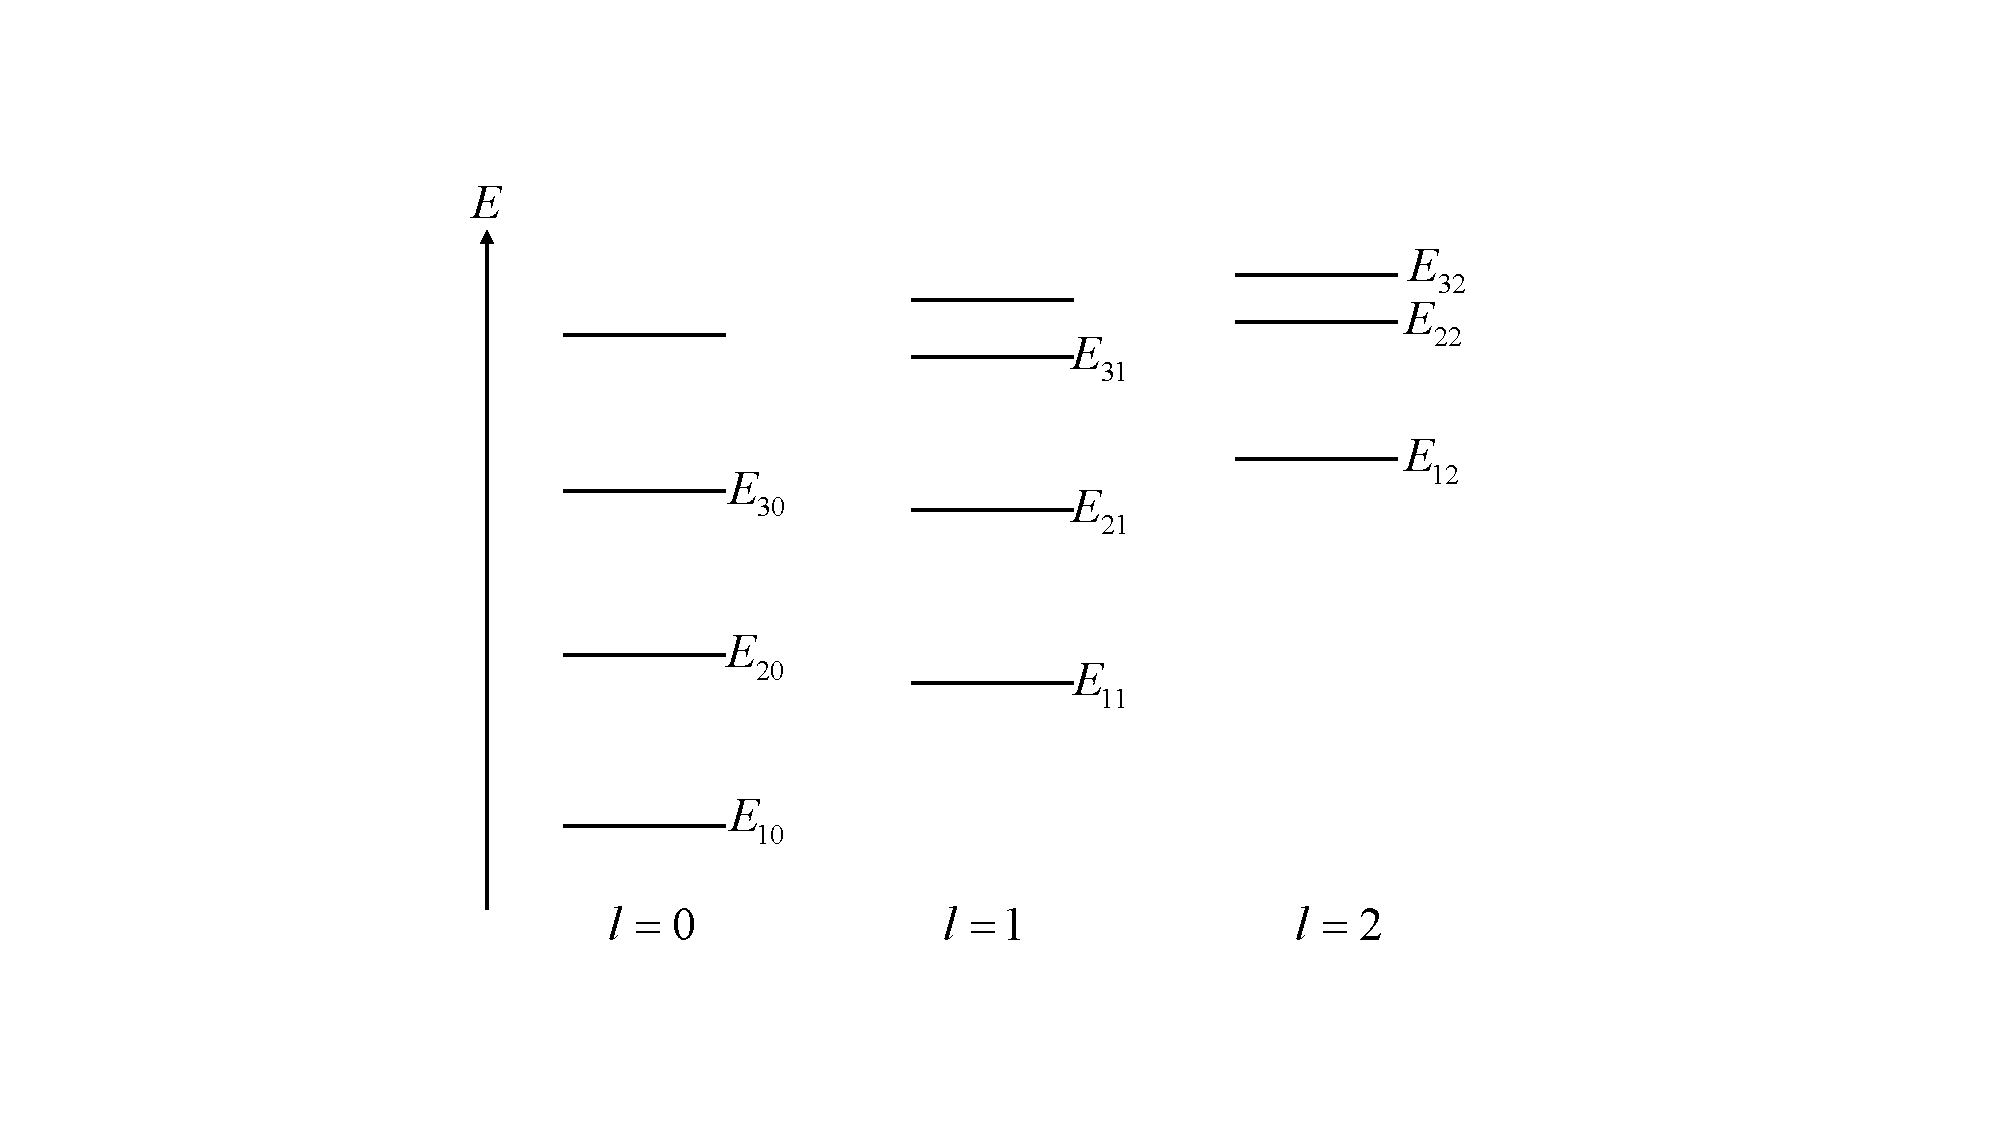
\includegraphics[width=6cm,clip]{QM file/figure/5-1}
	\caption{中心力场能级示意图}\label{fig.5-1}
\end{figure}

由于径向方程与$L_{z}$的量子数(磁量子数)$m$无关,因此能级$E_{nl}$($n=1,2,\cdots$为编号数)也与$m$无关.给定$l$后,$m$共有$(2l+1)$种取值,相应于$(2l+1)$种不同的状态[见\eqref{eq51.10}式],因此能级$E_{nl}$的简并度为$(2l+1)$.在具体问题中,属于不同$l$值的能级还可能出现重合,从而加大能级的简并度.氢原子和谐振子的能级都有这种“额外”的简并化.

{\heiti 4. 宇称性}

本征函数\eqref{eq51.10}式具有明确的宇称性.当$\boldsymbol{r}\rightarrow-\boldsymbol{r}$,$r$不变,$\theta\rightarrow\pi-\theta,\varphi\rightarrow\varphi+\pi$,径向波函数$R(r)$总是偶宇称,$Y_{lm}$的宇称则为$(-1)^{l}$,即
\begin{empheq}{equation}\label{eq51.23}
	Y_{lm}(\pi-\theta,\varphi+\pi)=(-1)^{l}Y_{lm}(\theta,\varphi)
\end{empheq}
这从\eqref{eq51.7}式及$P_{l}^{m}$的定义不难看出.因此\eqref{eq51.10}式的宇称为$(-1)^{l}$.属于相邻$l$的波函数宇称相反.基态属于$l=0$,为偶宇称.

{\heiti 5. 轨道磁矩}

\begin{wrapfigure}[14]{r}{4em}
	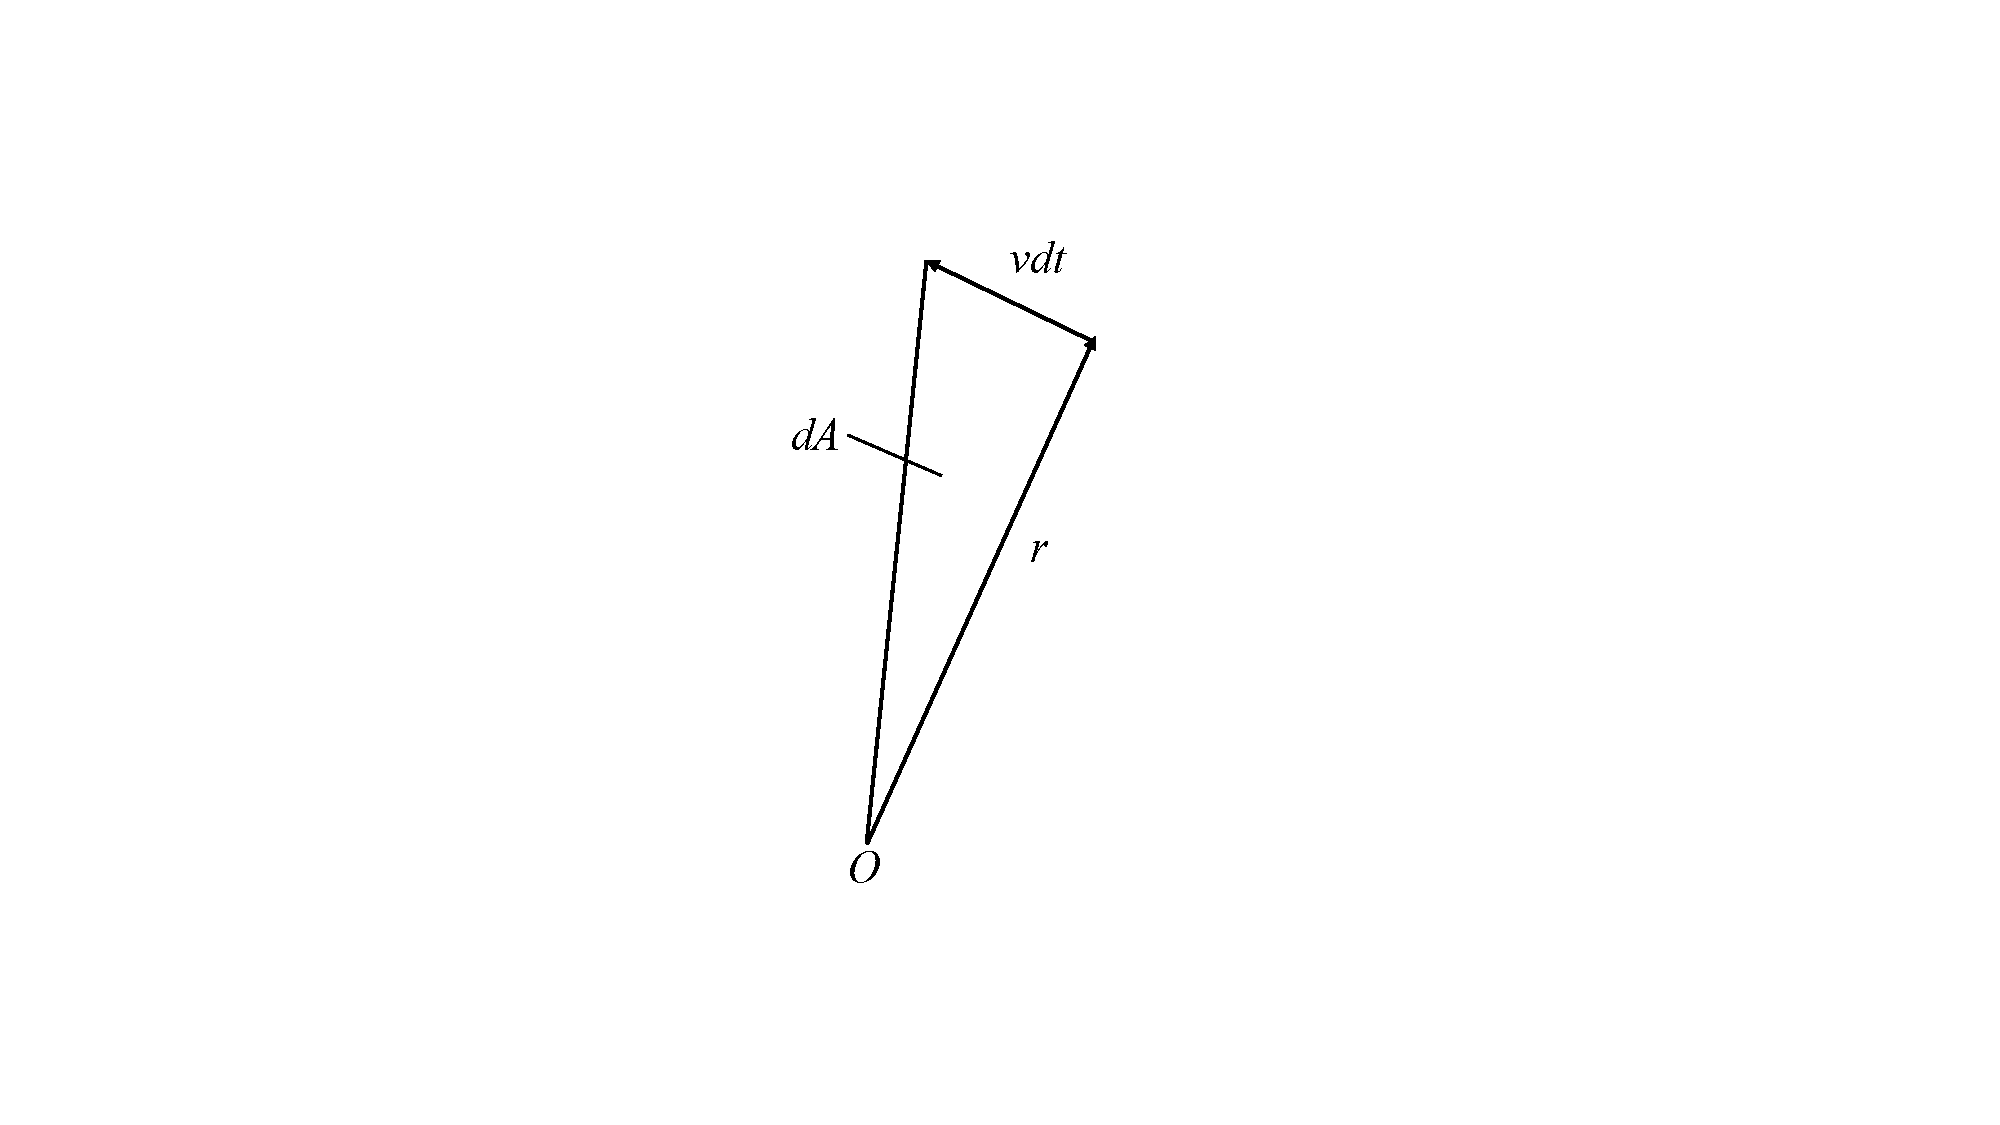
\includegraphics[width=2cm]{QM file/figure/5-2}
	\caption{}\label{fig.5-2}
\end{wrapfigure}
在经典力学中,质量为$\mu$电荷为$q$的粒子受中心力作用而沿平面闭合曲线作周期运动时,如图\ref{fig.5-2}所示,矢径$\boldsymbol{r}$的掠面速度为
\eqlong
\begin{empheq}{equation*}
	\frac{d\boldsymbol{A}}{dt}=\frac{1}{2}\boldsymbol{r}\times\boldsymbol{v}=\frac{1}{2\mu}\boldsymbol{r}\times\boldsymbol{p}=\frac{\boldsymbol{L}}{2\mu}
\end{empheq}
轨道曲线所围面积为
\begin{empheq}{equation}\label{eq51.24}
	\boldsymbol{A}=\oint d\boldsymbol{A}=\oint\frac{\boldsymbol{L}}{2\mu}dt=\frac{\tau}{2\mu}\boldsymbol{L}
\end{empheq}\eqnormal
其中$\boldsymbol{L}$为轨道角动量,$T$为周期.这种周期运动相当于一个环形电流回路,相应的等效电流为
\eqindent{9}
\begin{empheq}{equation}\label{eq51.25}
	I=\frac{q}{\tau}
\end{empheq}\eqnormal
等效磁矩为
\begin{empheq}{equation}\label{eq51.26}
	\boldsymbol{\mu}_{L}=\boldsymbol{IA}=\frac{q}{2\mu}\boldsymbol{L}\quad\text{国际单位制}
\end{empheq}
或
\begin{empheq}{equation*}\label{eq51.26'}
	\boldsymbol{\mu}_{L}=\frac{1}{c}\boldsymbol{IA}=\frac{q}{2\mu c}\boldsymbol{L}\quad\text{高斯单位制}	\tag{$5.1.26^{\prime}$}
\end{empheq}
在量子力学中,对于带电粒子的运动,轨道磁矩算符$\hat{\boldsymbol{\mu}}_{L}$就按\eqref{eq51.26}、\eqref{eq51.26'}式定义,其中$\boldsymbol{L}$理解为轨道角动量算符.当波函数为\eqref{eq51.10}式时,$L_{z}$取本征值$m\hbar$,$L_{x}$与$L_{y}$的平均值为0,因此$\boldsymbol{\mu}_{L}$的$z$分量取量子化的本征值:
\begin{empheq}{equation}\label{eq51.27}
	(\boldsymbol{\mu}_{L})_{z}=\frac{q\hbar}{2\mu}m\quad\text{国际单位制}
\end{empheq}
或
\begin{empheq}{equation*}\label{eq51.27'}
	(\boldsymbol{\mu}_{L})_{z}=\frac{q\hbar}{2\mu c}m\quad\text{高斯单位制}	\tag{$5.1.27^{\prime}$}
\end{empheq}
而$(\boldsymbol{\mu}_{L})_{x}$与$(\boldsymbol{\mu}_{L})_{y}$的平均值均等于零.

对于电子,电荷$q=-e$,质量$\mu=m_{e}$,如引入“玻尔磁子”:
\eqllong
\begin{empheq}{equation}\label{eq51.28}
	\mu_{B}=\frac{e\hbar}{2m_{e}}\quad\text{国际单位制},\quad\mu_{B}=\frac{e\hbar}{2m_{e}c}\text{高斯单位制}
\end{empheq}\eqnormal
则轨道磁矩的量子化本征值可以表示成
\begin{empheq}{equation}\label{eq51.29}
	(\boldsymbol{\mu}_{z})=-m\mu_{B},m=0,\pm1,\pm2,\cdots
\end{empheq}

{\heiti 6. 平均电流}

当粒子处于$\varPsi$态,$\S$\ref{sec:02.02}讲过的统计意义下的电流密度应该理解成平均电流密度,即
\begin{empheq}{equation}\label{eq51.30}
	j_{e}=-\frac{i\hbar}{2\mu}q(\varPsi^{*}\nabla\varPsi-\varPsi\nabla\varPsi^{*})
\end{empheq}
利用梯度算符的球坐标表示式[见附录\ref{A03}]
\begin{empheq}{equation}\label{eq51.31}
	\nabla=\boldsymbol{e}_{r}\frac{\partial}{\partial r}
	+\boldsymbol{e}_{\theta}\frac{1}{r}\frac{\partial}{\partial \theta}
	+\boldsymbol{e}_{\varphi}\frac{1}{r\sin\theta}\frac{\partial}{\partial \varphi}
\end{empheq}
$\boldsymbol{j}_{e}$可以表示成
\begin{empheq}{equation}\label{eq51.32}
	j_{e}=\boldsymbol{e}_{r}j_{r}+\boldsymbol{e}_{\theta}j_{\theta}+\boldsymbol{e}_{\varphi}j_{\varphi}
\end{empheq}
其中$\boldsymbol{e}_{r},\boldsymbol{e}_{\theta},\boldsymbol{e}_{\varphi}$中分别代表$\boldsymbol{r}$处沿半径方向、经线($\theta$增加方向)、纬线($\varphi$增加方向)方向的单位矢量,$j_{r},j_{\theta},j_{\varphi}$为$\boldsymbol{j}_{e}$在这三个方向的投影.即
\eqlong
\begin{empheq}{equation}\label{eq51.33}
	\begin{aligned}
		j_{e}&=-\frac{i\hbar}{2\mu}q(\varPsi^{*}\frac{\partial}{\partial r}\varPsi-\varPsi\frac{\partial}{\partial r}\varPsi^{*})	\\
		j_{\theta}&=-\frac{i\hbar}{2\mu}q\frac{1}{r}(\varPsi^{*}\frac{\partial}{\partial \theta}\varPsi-\varPsi\frac{\partial}{\partial \theta}\varPsi^{*})	\\
		j_{\varphi}&=-\frac{i\hbar}{2\mu}q\frac{1}{r\sin\theta}(\varPsi^{*}\frac{\partial}{\partial \varphi}\varPsi-\varPsi\frac{\partial}{\partial \varphi}\varPsi^{*})
	\end{aligned}
\end{empheq}
当波函数$\varPsi$为\eqref{eq51.10}式时,
\begin{empheq}{equation*}
	\varPsi(r,\theta,\varphi)=R(r)Y_{lm}(\theta,\varphi)=cR(R)P_{l}^{m}(\cos\theta)e^{im\varphi}
\end{empheq}\eqnormal
$\varPsi$中$\theta$部分$P_{l}^{m}(\cos\theta)$是实数,因此$j_{\theta}=0$.对于束缚态,径向波函数$R(r)$是实数,因此$j_{e}=0$.只有$j_{\varphi}\neq 0$中$\varphi$部分是$e^{im\varphi}$,因此
\begin{empheq}{equation*}
	\frac{\partial}{\partial \varphi}\varPsi=im\varphi,\quad \frac{\partial}{\partial \varphi}\varPsi^{*}=-im\varPsi^{*}
\end{empheq}\eqshort
\begin{empheq}{equation}\label{eq51.34}
	j_{\varphi}=\frac{\hbar q}{\mu}m\frac{\varPsi^{*}\varPsi}{r\sin\theta}
\end{empheq}\eqnormal
$j_{\varphi}$是$r,\theta$的函数,而与$\varphi$无关,平均电流沿各纬线流动,呈圆环状.早先安培曾假设原子中存在环状电流,现在得到了理论证明.如沿纬线取横截面元$rd\theta dr$,形成细圆环,其体积为
\eqlong
\begin{empheq}{equation}\label{eq51.35}
	d\tau=2\pi r\sin\theta\cdot rd\theta dr=2\pi r^{2}\sin\theta d\theta dr
\end{empheq}
环中平均电流为
\begin{empheq}{equation}\label{eq51.36}
	dI=j_{\varphi}rd\theta dr=\frac{\hbar q}{\mu}m\frac{\varPsi^{*}\varPsi}{\sin\theta}d\theta dr
\end{empheq}
$dI$对等效磁矩(平均值)的贡献为
\begin{empheq}{equation}\label{eq51.37}
	dM_{z}=\frac{1}{c}dI\cdot\pi(r\sin\theta)^{2}=m\frac{\hbar q}{2\mu c}\varPsi^{*}d\tau
\end{empheq}
各细电流环贡献的总等效磁矩(平均值)为
\begin{empheq}{equation}\label{eq51.38}
	M_{z}=\int dM_{z}=m\frac{\hbar q}{2\mu c}\int\varPsi^{*}\varPsi d\tau=m\frac{\hbar q}{2\mu c}
\end{empheq}\eqnormal
(高斯单位制)这正是\eqref{eq51.27'}式给出的轨道磁矩$(\boldsymbol{\mu}_{L})_{z}$的本征值.






% 自由粒子
\section[自由粒子]{自由粒子} \label{sec:05.02} % 
% \makebox[5em][s]{} % 短题目拉间距

自由运动的粒子,总能等于动能(取势能$V=0$),
\begin{empheq}{equation}\label{eq52.1}
	\hat{H}=\frac{\hat{\boldsymbol{p}}^{2}}{2\mu}=-\frac{\hbar^{2}}{2\mu}\nabla^{2}
\end{empheq}
主要守恒量有$\boldsymbol{H},\boldsymbol{p},\boldsymbol{L}$等作为守恒量完全集,可取$(p_{x},p_{y},p_{z}$或$(H,\boldsymbol{L}^{2},L_{z})$.前者的共同本征函数就是自由粒子平面波(参看$\S$\ref{sec:03.05})
\begin{empheq}{equation}\label{eq52.2}
	\varPsi_{\boldsymbol{p}}(\boldsymbol{r})=(2\pi\hbar)^{-\frac{3}{2}}e^{i\boldsymbol{p}\cdot\boldsymbol{r}/\hbar}
\end{empheq}
本节专门讨论$(\hat{\boldsymbol{H}},\hat{\boldsymbol{L}}^{2},\hat{L}_{z})$的共同本征函数,称为自由粒子球面波.按照\eqref{eq51.10}、\eqref{eq51.13}、\eqref{eq51.14}式,波函数可以表示成
\begin{empheq}{equation}\label{eq52.3}
	\varPsi=R_{l}(r)Y_{lm}(\theta,\varphi)=\frac{u_{l}(r)}{kr}Y_{lm}(\theta,\varphi)
\end{empheq}
$u_{l}(r)$满足径向方程
\begin{empheq}{equation}\label{eq52.4}
	\frac{d^{2}}{dr^{2}}u_{l}+\bigg[\frac{2\mu E}{\hbar^{2}}-\frac{l(l+1)}{r^{2}}\bigg]u_{l}=0
\end{empheq}
令
\begin{empheq}{equation}\label{eq52.5}
	k=\frac{\sqrt{2\mu E}}{\hbar},\quad kr=\rho
\end{empheq}
$E,k$可以连续变化(取正值),\eqref{eq52.4}式简化成
\begin{empheq}{equation*}\label{eq52.4'}
	\rho^{2}\frac{d^{2}u_{l}}{d\rho^{2}}+[\rho^{2}-l(l+1)]u_{l}=0
	\tag{$5.2.4^{\prime}$}
\end{empheq}
下面求$u_{l}$及$R_{l}(r)$.根据\eqref{eq51.18}式,令
\begin{empheq}{equation}\label{eq52.6}
	u_{l}=(-1)^{l}\rho^{l+1}W_{l}(\rho)
\end{empheq}
代入\eqref{eq52.4'}式,得到$W_{l}$满足的方程
\begin{empheq}{equation}\label{eq52.7}
	W_{l}^{\prime\prime}+2(l+1)\frac{W_{l}^{\prime}}{\rho}+W_{l}=0
\end{empheq}
再令
\begin{empheq}{equation}\label{eq52.8}
	v_{l}=\frac{W_{l}^{\prime}}{\rho}=\frac{1}{\rho}\frac{dW_{l}}{d\rho}
\end{empheq}
则
\begin{empheq}{equation*}
	W_{l}^{\prime}=\rho v_{l},\quad W_{l}^{\prime\prime}=\rho v_{l}^{\prime}+v_{l}
\end{empheq}
代入\eqref{eq52.7}式,得到
\begin{empheq}{equation*}
	\rho v_{l}^{\prime}+(2l+3)v_{l}+W_{l}=0
\end{empheq}
再微分一次,并用$\rho$除,得到
\begin{empheq}{equation}\label{eq52.9}
	v_{l}^{\prime\prime}+2(l+2)\frac{v_{l}^{\prime}}{\rho}+v_{l}=0
\end{empheq}
比较\eqref{eq52.7}、\eqref{eq52.9}式,可见
\begin{empheq}{equation}\label{eq52.10}
	W_{l+1}=v_{l}=\frac{1}{\rho}\frac{dW_{l}}{d\rho}
\end{empheq}
这是各$W_{l}$之间的递推公式.$l=0$时,\eqref{eq52.4'}式成为
\eqshort
\begin{empheq}{equation}\label{eq52.11}
	u_{0}^{\prime\prime}+u_{0}=0
\end{empheq}\eqnormal
其独立解为
\begin{empheq}{equation}\label{eq52.12}
	u_{0}=\sin\rho,\cos\rho\text{或}e^{i\varphi},e^{-i\varphi}
\end{empheq}
相应的$R_{0}$及$W_{0}$为
\eqlong
\begin{empheq}{equation}\label{eq52.13}
	R_{0}=W_{0}=\frac{u_{0}}{\rho}=\frac{\sin\rho}{\rho},\frac{\cos\rho}{\rho}\text{或}\frac{e^{i\varphi}}{\rho},\frac{e^{-i\varphi}}{\rho}
\end{empheq}\eqnormal
前两种为驻波,后两种为行波这四种解在$r>O$处均满足能量本征方程$\hat{H}\varPsi=E\varPsi$,亦即
\eqshort
\begin{empheq}{equation}\label{eq52.14}
	\nabla^{2}\varPsi+k^{2}\varPsi=0
\end{empheq}\eqnormal
$\bigg($注意,$l=0$时$Y_{00}=\frac{1}{\sqrt{4\pi}}$,$\varPsi$与$R_{0}$只相差一个常系数.$\bigg)$但是,在全空间($r\rightarrow 0$也包括在内)满足\eqref{eq52.14}式的解,当$l=0$时只有\eqref{eq52.13}式的第一种\footnote{$r\rightarrow0$处另外三种解均与$\frac{1}{r}$成比例,不满足\eqref{eq52.14}式.理由参看本章\ref{F.5-1}注.},即
\begin{empheq}{equation}\label{eq52.15}
	R_{0}=W_{0}=\frac{\sin\rho}{\rho}\equiv j_{0}(\rho)
\end{empheq}
利用\eqref{eq52.10}式及\eqref{eq52.6}式, 即可求出
\begin{empheq}{equation*}
	W_{l}=\bigg(\frac{1}{\rho}\frac{d}{d\rho}\bigg)^{l}\bigg(\frac{\sin\rho}{\rho}\bigg)
\end{empheq}\eqlong
\begin{empheq}{align}\label{eq52.16}
	R_{l}(r)&=\frac{u_{l}}{\rho}=(-1)^{l}\rho^{l}W_{l}	\nonumber\\
	&=(-1)^{l}\rho^{l}\bigg(\frac{1}{\rho}\frac{d}{d\rho}\bigg)^{l}\bigg(\frac{\sin\rho}{\rho}\bigg)\equiv j_{l}(\rho)
\end{empheq}
\eqref{eq52.16}式称为球贝塞耳函数,它和第一类贝塞耳函数$J_{\nu}(\rho)$的关系是
\begin{empheq}{equation}\label{eq52.17}
	j_{l}(\rho)=\sqrt{\frac{\pi}{2\rho}}J_{l+\frac{1}{2}}(\rho),\quad l=0,1,2,\cdots
\end{empheq}
这是唯一能够表示成初等函数的贝塞耳函数.

许多问题中常用到$j_{l}(\rho)$的渐近表示,这可以利用\eqref{eq52.16}式求出.当$\rho\rightarrow\infty(\rho\geqslant l)$,略去$\rho^{-2}$以下小量,并利用公式
\begin{empheq}{equation*}
	\frac{d}{d\rho}\sin\rho=\cos\rho=-\sin\bigg(\rho-\frac{\pi}{2}\bigg)
\end{empheq}\eqnormal
容易得出
\begin{empheq}{equation}\label{eq52.18}
	j_{l}(\rho)\sim\frac{1}{\rho}\sin\bigg(\rho-\frac{l\pi}{2}\bigg),\quad \rho\rightarrow\infty
\end{empheq}
当$\rho\rightarrow 0$,利用公式
\begin{empheq}{align*}
	\frac{\sin\rho}{\rho}=&\sum_{n=0}^{\infty}\frac{(-1)^{n}}{(2n+1)!}\rho^{2n}	\\
	\frac{1}{\rho}\frac{d}{d\rho}&=2\frac{d}{d(\rho^{2})}
\end{empheq}
由\eqref{eq52.16}式易得
\eqlong
\begin{empheq}{equation}\label{eq52.19}
	j_{l}(\rho)\rightarrow\frac{\rho^{l}}{(2l+1)!!}=\frac{\rho^{l}}{1\cdot3\cdot5\cdot\cdots\cdot(2l+1)}
\end{empheq}

作为径向波函数,$j_{l}(kr)$显然是不能归一化的,这是游离态波函数的特点.至于$l$相同,能量为$E=\frac{\hbar^{2}k^{2}}{2\mu}$和$E^{\prime}=\frac{\hbar^{2}k^{\prime2}}{2\mu}$的两个径向波函数$j_{l}(kr)$和$j_{l}(k^{\prime}r)$,则有下列正交归一性
\begin{empheq}{align}\label{eq52.20}
	&\int_{0}^{\infty}j_{l}(kr)j_{l}(k^{\prime}r)r^{2}dr	\nonumber\\
	\approx&\frac{1}{kk^{\prime}}\int_{0}^{\infty}\sin\bigg(kr-\frac{l\pi}{2}\bigg)\sin\bigg(k^{\prime}r-\frac{l\pi}{2}\bigg)dr	\nonumber\\
	=&\frac{1}{2kk^{\prime}}\int_{0}^{\infty}[\cos(k-k^{\prime})r+(-1)^{l+1}\cos(k+k^{\prime})r]dr	\nonumber\\
	=&\frac{\pi}{2kk^{\prime}}\delta(k-k^{\prime})
\end{empheq}
计算中利用了渐近公式\eqref{eq52.18}以及
\begin{empheq}{align}\label{eq52.21}
	\delta(k-k^{\prime})&=\frac{1}{2\pi}\int_{-\infty}^{\infty}e^{i(k-k^{\prime})x}dx	\nonumber\\
	&=\frac{1}{\pi}\int_{0}^{\infty}\cos(k-k^{\prime})xdx
\end{empheq}\eqnormal

\example 将沿$z$方向传播的平面波(动量$p_{z}=\hbar k$)$e^{ikz}$展开成球面波的叠加.

\solution 平面波$e^{ikz}$中是\eqref{eq52.14}式的一个特解,它是$(\hat{p}_{x},\hat{p}_{y},\hat{p}_{z})$的共同本征函数.也是$\hat{L}_{z}$的本征函数,
\begin{empheq}{equation*}
	\hat{L}_{z}e^{ikz}=-i\hbar\frac{\partial}{\partial\varphi}e^{ikr\cos\theta}=0
\end{empheq}
即$L_{z}$的本征值为0.但$e^{ikz}$并非$\hat{\boldsymbol{L}}^{2}$的本征函数.将$e^{ikz}$展开成各$Y_{lm}$的线性叠加,必然具有下列形式
\begin{empheq}{equation}\label{eq52.22}
	e^{ikz}=e^{ikr\cos\theta}=\sum_{l=0}^{\infty}C_{l}j_{l}(kr)Y_{l0}(\theta)
\end{empheq}
由于
\begin{empheq}{equation}\label{eq52.23}
	Y_{l0}(\theta)=\sqrt{\frac{2l+1}{4\pi}}P_{l}(\cos\theta)
\end{empheq}
所以\eqref{eq52.22}式也可写成
\begin{empheq}{equation*}\label{eq52.22'}
	e^{ikz}=e^{ikr\cos\theta}=\sum_{l=0}^{\infty}C_{l}^{\prime}j_{l}(kr)P_{l}(\cos\theta)
	\tag{$5.2.22^{\prime}$}
\end{empheq}
其中
\begin{empheq}{equation*}
	C_{l}^{\prime}=\sqrt{\frac{2l+1}{4\pi}}C_{l}
\end{empheq}
为待定系数.将\eqref{eq52.22'}左端展开成幕级数,
\begin{empheq}{equation}\label{eq52.24}
	e^{ikr\cos\theta}=\sum_{0}^{\infty}\frac{1}{l!}(ikr\cos\theta)^{l}
\end{empheq}
其中$kr$的幕次总是和$\cos\theta$的幕次相同.

根据$P_{l}$的定义
\eqlong
\begin{empheq}{equation*}
	P_{l}(\cos\theta)=\frac{1}{2^{l}l!}\bigg(\frac{d}{d\cos\theta}\bigg)^{l}(\cos^{2}\theta-1)^{l}
\end{empheq}\eqnormal
最高次项$(\cos\theta)^{l}$的系数为
\begin{empheq}{equation*}
	\frac{(2l)(2l-1)\cdots(l+1)}{2^{l}l!}
\end{empheq}
而在$j_{l}(kr)$的级数表示式中,最低幕次为$(kr)^{l}$,系数为[见\eqref{eq52.19}式]$\frac{1}{(2l+1)!!}$.因此\eqref{eq52.22'}式右端$(kr\cos\theta)^{l}$项系数为
\begin{empheq}{equation*}
	\frac{C_{l}^{\prime}(2l)(2l-1)\cdots(l+1)}{2^{l}l!(2l+1)!!}
\end{empheq}
与\eqref{eq52.24}式比较,即得
\eqlong
\begin{empheq}{equation}\label{eq52.25}
	C_{l}^{\prime}=\frac{i^{l}2^{l}(2l+1)!!}{(2l)(2l-1)\cdots(l+1)}=(2l+1)i^{l}
\end{empheq}
代入\eqref{eq52.22'}式,即得
\begin{empheq}{equation}\label{eq52.26}
	e^{ikz}=\sum_{l=0}^{\infty}(2l+1)i^{l}j_{l}(kr)P_{l}(\cos\theta)
\end{empheq}
这就是所求展开式.当$kr\rightarrow\infty$,利用\eqref{eq52.18}式可得
\begin{empheq}{equation}\label{eq52.27}
	e^{ikz}\sim\frac{1}{kr}\sum_{l=0}^{\infty}(2l+1)i^{l}\sin\bigg(kr-\frac{l\pi}{2}\bigg)P_{l}(\cos\theta)
\end{empheq}\eqnormal
这个结果对于散射问题很有用.

% 球型势阱
\starthis\section[球型势阱]{球型势阱} \label{sec:05.03} % 
% \makebox[5em][s]{} % 短题目拉间距

{\heiti 1. 无限深球形势阱}

设粒子被无限深球形势阱
\begin{empheq}{equation}\label{eq53.1}
	{V(r)=}
	\begin{dcases}
		0,\quad r<a	\\
		\infty,\quad r\geqslant a
	\end{dcases}
\end{empheq}
限制在球内$(r<a)$运动.球内薛定谔方程与自由粒子相同,球外边界条件为
\begin{empheq}{equation}\label{eq53.2}
	r\geqslant a,\quad \varPsi=0
\end{empheq}
由于是中心力场,轨道角动址$\boldsymbol{L}$是守恒量,$(\hat{H},\hat{\boldsymbol{L}}^{2},\hat{L}_{z})$的共同本征函数可以表示成(略去归一化常数)
\begin{empheq}{equation}\label{eq53.3}
	\varPsi(r,\theta,\varphi)=j_{l}(kr)Y_{lm}(\theta,\varphi),\quad r<a
\end{empheq}
其中
\begin{empheq}{equation}\label{eq53.4}
	k=\frac{\sqrt{2\mu E}}{\hbar}
\end{empheq}
边界条件\eqref{eq53.2}具体表现为
\begin{empheq}{equation}\label{eq53.5}
	j_{l}(ka)=0
\end{empheq}
这也就是决定能级的条件.$j_{l}(x)$的零点记成$x_{nl}$($n=1,2,\cdots$是零点的序数),其值可以从贝塞耳函数表查得,如表\ref{lab.5-1}.$k$和$E$的特征值由$x_{nl}$决定,
\begin{empheq}{equation}\label{eq53.6}
	k_{nl}=\frac{x_{nl}}{a}
\end{empheq}
\begin{empheq}{equation}\label{eq53.7}
	E_{nl}=\frac{\hbar^{2}}{2\mu}k_{nl}^{2}=\frac{\hbar^{2}}{2\mu a^{2}}x_{nl}^{2}
\end{empheq}
由于各$j_{l}$没有相同的零点,因此属于$l=0,1,2\cdots$的各组能级互不相同.能级$E_{nl}$的简并度等于$(2l+1)$,相应于$(2l+1)$种$m$值,
\begin{empheq}{equation*}
	m=0,\pm1,\pm2,\cdots,\pm l
\end{empheq}
按照光谱学的习惯,各$l$值用字母表记:

\begin{empheq}{alignat*=7}
	l &\quad 0 &\quad 1 &\quad 2 &\quad 3 &\quad 4 &\quad 5	\\
	\text{字母} &\quad s &\quad p &\quad d &\quad f &\quad g &\quad h	\\
\end{empheq}
能级$E_{10}$已成$1\si{s}$,$E_{23}$记成$2\si{f}$,等等.

\begin{table}[!h]
	\begin{center}
		\caption{$\dfrac{x_{nl}}{\pi}$的数值}\label{lab.5-1}
		\setlength{\tabcolsep}{4mm}	% 调节表格尺寸
		%\resizebox{h-length}{v-length}{text}
		\begin{tabular}{c|c|c|c|c|c}
			\hline 
			\diagbox{$l$}{$n$} & 1 & 2 & 3 & 4 & 5	\\	\hline
			0 & 1 & 2 & 3 & 4 & 5	\\	\hline
			1 & 1.4303 & 2.4590 & 3.4709 & 4.4774 & 5.4816	\\	\hline
			2 & 1.8346 & 2.8950 & 3.9225 & 4.9386 & 5.9489	\\	\hline
			3 & 2.2243 & 3.3159 & 4.3602 & 5.3870 & 6.4050	\\	\hline
			4 & 2.6046 & 3.7258 & 4.7873 & 5.8255 & 6.8518	\\	\hline
			5 & 2.9780 & 4.1274 & 5.2059 & 6.2558 & 7.2908	\\	\hline
			6 & 3.3464 & 4.5224 & 5.6176 & 6.6793 & 7.7231	\\	\hline
		\end{tabular}
	\end{center}
\end{table}

由表\ref{lab.5-1}可以看出,能级由低到高的次序(即$x_{nl}$的次序)是
\begin{empheq}{equation*}
	1\si{s},1\si{p},1\si{d},2\si{s},1\si{f},2\si{p},1\si{g},2\si{d},1\si{h},3\si{s},2\si{f},\cdots
\end{empheq}

s态$(l=0)$的能级条件是
\begin{empheq}{equation*}
	j_{0}(x)=\frac{\sin x}{x}=0,\quad x=ka
\end{empheq}
解为
\begin{empheq}{align}\label{eq53.8}
	x_{n0}&=n\pi,\quad n=1,2,3,\cdots	\nonumber\\
	k_{n0}&=\frac{n\pi}{a},\quad E_{n0}=n^{2}\frac{\pi^{2}\hbar^{2}}{2\mu a^{2}}
\end{empheq}
这结果与一维无限深势阱相同,原因是,$l=0$时离心势能为0,$u(r)=n\varPsi$所满足的径向方程以及边界条件均类似于一维无限深势阱问题.基态能级是
\begin{empheq}{equation}\label{eq53.9}
	E_{10}=\frac{\pi^{2}\hbar^{2}}{2\mu a^{2}}
\end{empheq}
\eqref{eq53.7}式也可以写成
\begin{empheq}{equation*}\label{eq53.7'}
	E_{nl}=\bigg(\frac{x_{nl}}{\pi}\bigg)E_{10}
	\tag{$5.3.7^{\prime}$}
\end{empheq}
由表\ref{lab.5-1}可见,能级分布不是等距离的,但最低的几个能级分布比较均匀.高激发态的情况就大不一样.根据$j_{l}$的渐近公式[\eqref{eq52.18}式]易见其零点约为
\begin{empheq}{equation}\label{eq53.10}
	x_{nl}\approx \bigg(n+\frac{l}{2}\bigg)\pi
\end{empheq}
[当$n>l$,\eqref{eq53.10}式的近似程度就相当好,参看表\ref{lab.5-1}]因此
\begin{empheq}{equation*}
	x_{nl}\approx x_{n+1,l-2}\approx x_{n+2,l-4}\approx \cdots
\end{empheq}
能级出现近似简并的微妙情形.这种近似简并在$n<l$时也偶尔出现,如$E_{15}$和$E_{30}$,$E_{23}$和$E_{16}$,$E_{17}$和$E_{24}$,等等.

{\heiti 2.氘核}

氘核是质子和中子在核力(强作用)作用下形成的束缚态,而且是唯一的束缚态.根据实验测定,氘核的结合能为$|E|=\num{2.237}\si{MeV}$.

\begin{wrapfigure}[9]{r}{7em}
	\centering
	\small
	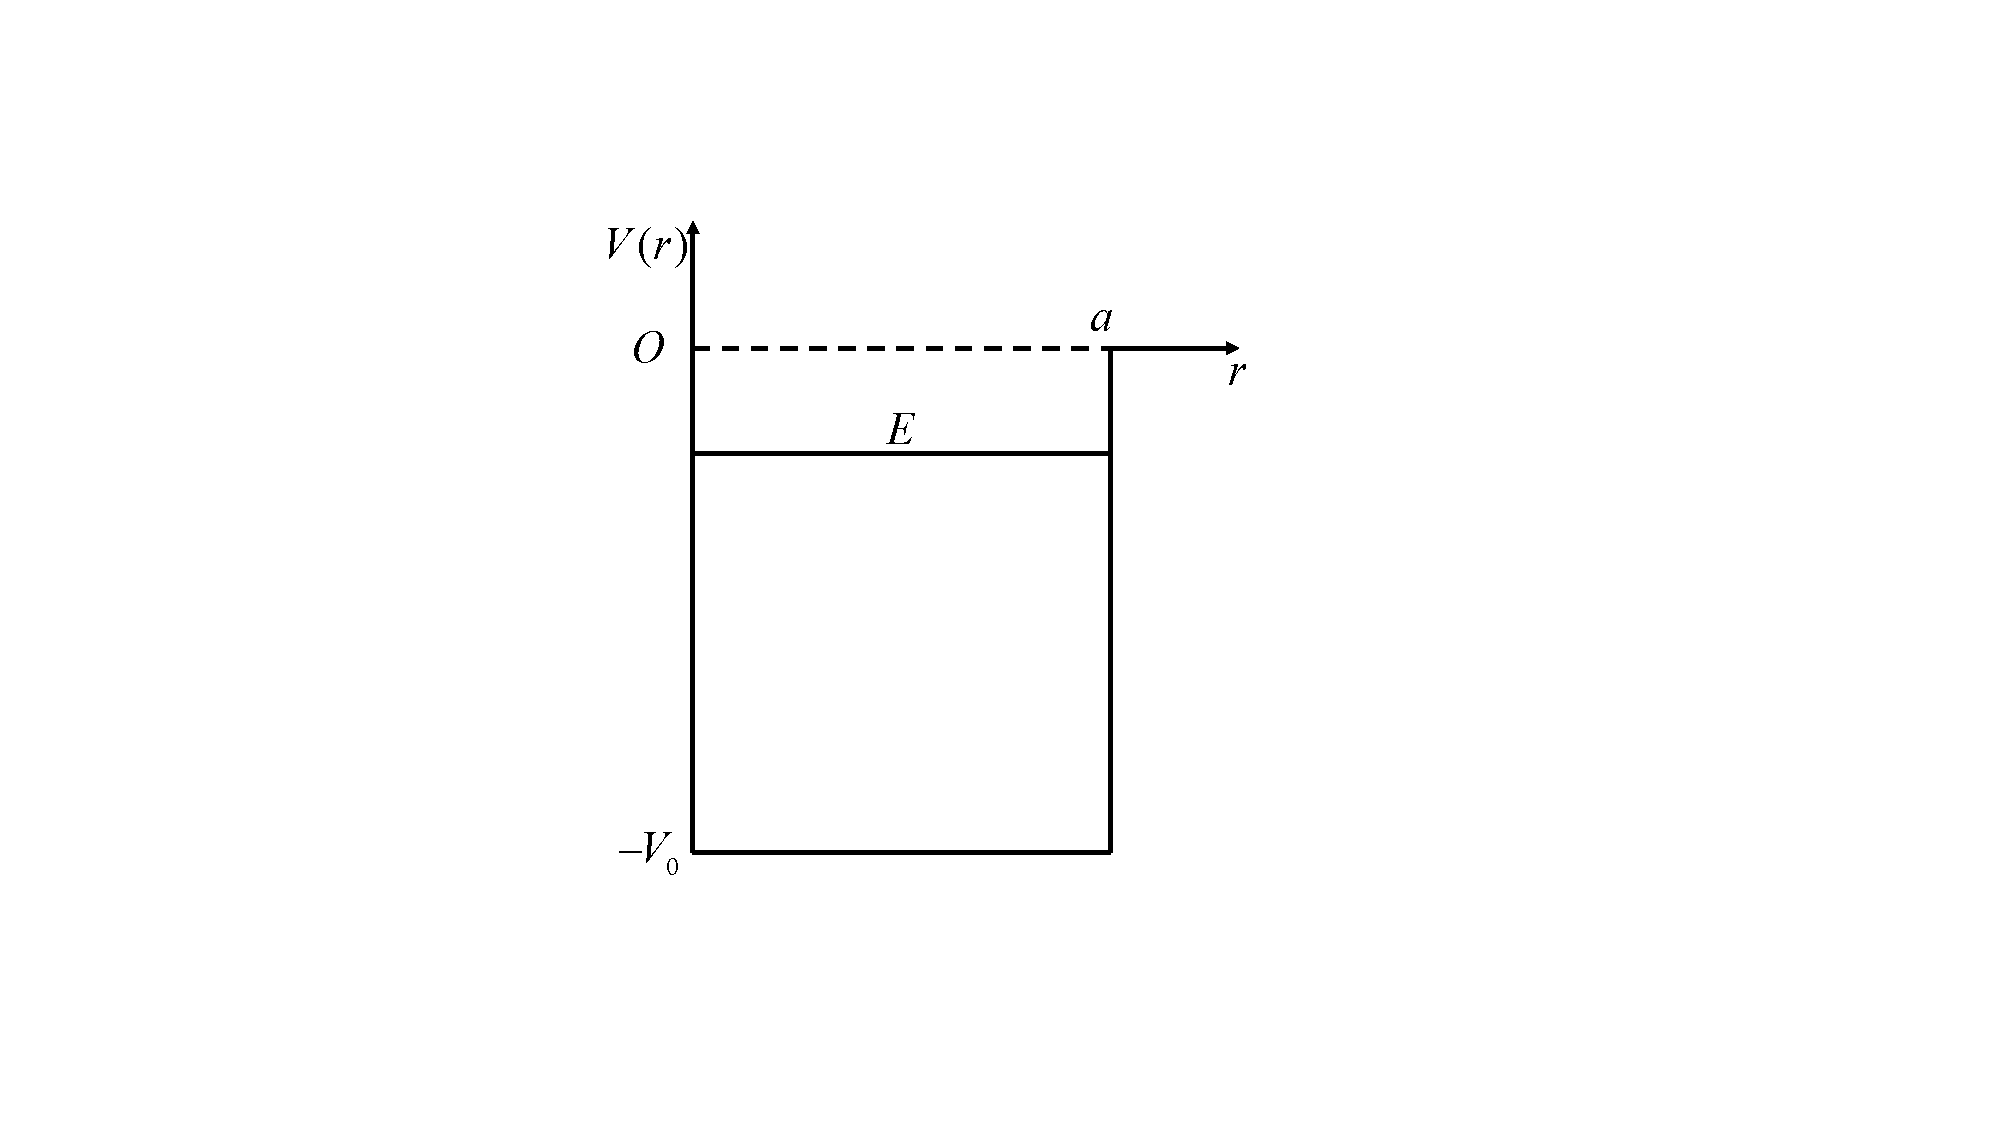
\includegraphics[width=3cm]{QM file/figure/5-3}
	\caption{}\label{fig.5-3}
\end{wrapfigure}
核力是短程力,力程约2\si{fm},作用强度约$20\sim 30 \si{MeV}$,近似地可以用图\ref{fig.5-3}所示的球形势阱表示质子-中子之间的核力作用势,
\eqlong
\begin{empheq}{equation}\label{eq53.11}
	{V(r)=}
	\begin{dcases}
		-V_{0},\quad r\leqslant a	\\
		0,\quad r>a
	\end{dcases}
\end{empheq}\eqshort
$a$为力程,$V_{0}$为作用强度.利用结合能的实验值可以求出$V_{0}$与$a$的依赖关系,如下.

氘核是稳定的,相当于基态,角量子数$l=0$,波函数可以写成(不考虑归一化)
\begin{empheq}{equation}\label{eq53.12}
	\varPsi(r)=\frac{u(r)}{r}
\end{empheq}\eqnormal
$u(r)$满足径向方程[\eqref{eq51.14}式,$l=0$]
\begin{empheq}{equation}\label{eq53.13}
	\bigg[-\frac{\hbar^{2}}{2\mu}\frac{d^{2}}{dr^{2}}+V(r)-E\bigg]u(r)=0
\end{empheq}
亦即
\begin{empheq}{equation*}\label{eq53.13'}
	{}
	\begin{dcases}
		\frac{d^{2}}{dr^{2}}u+k^{2}u=0,\quad r\leqslant a	\\
		\frac{d^{2}}{dr^{2}}u-\beta^{2}u=0,\quad r>a
	\end{dcases}
	\tag{$5.3.13^{\prime}$}
\end{empheq}
其中
\begin{empheq}{equation}\label{eq53.14}
	k=\frac{\sqrt{2\mu(V_{0}+E)}}{\hbar},\quad \beta=\frac{\sqrt{-2\mu E}}{\hbar}(E<0)
\end{empheq}
边界条件为
\begin{empheq}{equation}\label{eq53.15}
	r\rightarrow 0,\quad u\rightarrow 0;\quad r\rightarrow \infty,\quad u\rightarrow 0
\end{empheq}
\eqref{eq53.13'}式满足这边界条件的解为
\begin{empheq}{equation}\label{eq53.16}
	{u(r)=}
	\begin{dcases}
		\sin kr,\quad r\leqslant a	\\
		Ce^{-\beta r}, \quad r>a
	\end{dcases}
\end{empheq}
$r=a$处,$\frac{u^{\prime}}{u}$应该连续,由此求得能级公式
\begin{empheq}{equation}\label{eq53.17}
	\cot ka=-\frac{\beta}{k}
\end{empheq}
这公式类似于一维方势阱奇宇称态的能级公式,上式等价于
\begin{empheq}{equation}\label{eq53.18}
	\sin^{2}ka=\frac{k^{2}}{k^{2}+\beta^{2}}=1+\frac{E}{V_{0}}
\end{empheq}
对于氘核,$E=-\num{2.237}\si{MeV}$,$\mu$应该取为质子-中子体系的约化质量,
\begin{empheq}{align}\label{eq53.19}
	\mu=&\frac{m_{0}m_{p}}{m_{n}+m_{p}}\approx\frac{m_{p}}{2},\quad 2\mu c^{2}\approx 938\si{MeV}	\nonumber\\
	k^{2}&=\frac{2\mu(V_{0}+E)}{\hbar^{2}}=\frac{2\mu c^{2}(V_{0}+E)}{\hbar^{2}c^{2}}
\end{empheq}
\begin{table}[!h]
	\begin{center}
		\caption{}\label{lab.5-2}
		\setlength{\tabcolsep}{8mm}	% 调节表格尺寸
		%\resizebox{h-length}{v-length}{text}
		\begin{tabular}{c|c|c|c}
			\hline 
			$V_{0}/$\si{MeV} & 30 & 25 & 20 	\\	\hline
			$a/$\si{fm} & 2.26 & 2.53 & 2.92 	\\	\hline
		\end{tabular}
	\end{center}
\end{table}
在\eqref{eq53.18}、\eqref{eq53.19}式中,取实验值$E=\num{-2.237} \si{MeV}$,再指定一个$V_{0}$值,由\eqref{eq53.19}式算出$k$,由\eqref{eq53.18}式算出$ka$,从而求出与$V_{0}$相应的$a$值.结果如表\ref{lab.5-2}.

其中前二组数据比较接近于用其他方法(例如散射实验)确定的数值.






% 粒子在库仑场中的运动(束缚态)
\section[粒子在库仑场中的运动(束缚态)]{粒子在库仑场中的运动(束缚态)} \label{sec:05.04} % 
% \makebox[5em][s]{} % 短题目拉间距

\blfootnote{* 涉及库仑力作用$e^{2}/4\pi\varepsilon_{0}$简记为$\e^{2}$}
电子在原子核的库仑场中形成的束缚态,是原子和分子结构的基础,以$Ze$表示原子核电荷,$-e$表示电子电荷,原子核对电子的库仑作用势$^{*}$为
\begin{empheq}{equation}\label{eq54.1}
	V(r)=-\frac{Z\e^{2}}{r}
\end{empheq}
如略去原子核的运动,则电子的哈密顿算符可以写成
\begin{empheq}{equation}\label{eq54.2}
	\hat{H}=\hat{T}+\hat{V}=-\frac{\hbar^{2}}{2\mu}\nabla^{2}-\frac{Z\e^{2}}{r}
\end{empheq}
$\mu$为电子质置\footnote{严格说,原子核-电子体系应该作为二体问题处理,\eqref{eq54.2}式是电子对于核的相对运动哈密顿算符,其中$\mu$为折合质量.详细讨论请看$\S$\ref{sec:10.01}}.根据$\S$\ref{sec:05.01}的讨论,$(\hat{H},\hat{\boldsymbol{L}}^{2},\hat{L}_{z})$的共同本征函数可以表示成
\begin{empheq}{equation}\label{eq54.3}
	\varPsi=R(r)Y_{lm}(\theta,\varphi)=\frac{u(r)}{r}Y_{lm}(\theta,\varphi)
\end{empheq}
代入能量本征方程
\begin{empheq}{equation*}
	\hat{H}\varPsi=E\varPsi
\end{empheq}
得到径向方程
\begin{empheq}{equation}\label{eq54.4}
	\frac{d^{2}u}{dr^{2}}+\bigg[\frac{2\mu E}{\hbar^{2}}+\frac{2\mu Z\e^{2}}{\hbar^{2}}\frac{1}{r}-\frac{l(l+1)}{r^{2}}\bigg]u=0
\end{empheq}
只讨论束缚态,$E<0$.$\S$\ref{sec:05.01}已经一般地证明$u(r)$具有近似性质
\begin{empheq}{align}\label{eq54.5}
	r&\rightarrow 0,u(r)\sim Cr^{l+1}	\nonumber\\
	r&\rightarrow\infty,u(r)\sim C_{3}e^{-\alpha r},\alpha=\frac{\sqrt{-2\mu E}}{\hbar}
\end{empheq}
因此,令
\begin{empheq}{equation}\label{eq54.6}
	u(r)=Cr^{l+1}F(r)e^{-\alpha r}
\end{empheq}
其中$C$为归一化常数,$F(r)$为待定函数,$r\rightarrow 0$处$F\rightarrow 1$,将变换\eqref{eq54.6}式代入\eqref{eq54.6}式,得到$F(r)$满足的方程为
\eqllong
\begin{empheq}{equation}\label{eq54.7}
	r\frac{d^{2}F}{dr^{2}}+(2l+2-2\alpha r)\frac{dF}{dr}+\bigg[\frac{2\mu Z\e^{2}}{\hbar^{2}}-(2l+2)\alpha\bigg]F=0
\end{empheq}\eqnormal
引入无量纲变量
\begin{empheq}{equation}\label{eq54.8}
	\xi=2\alpha r=\frac{2}{\hbar}\sqrt{-2\mu Er}
\end{empheq}
并用$2\alpha$除\eqref{eq54.7}式,可以简化成
\eqlong
\begin{empheq}{equation}\label{eq54.9}
	\xi\frac{d^{2}F}{d\xi^{2}}+(2l+2-\xi)\frac{dF}{d\xi}-\bigg(l+1-\frac{\mu Z\e^{2}}{\alpha\hbar^{2}}\bigg)F=0
\end{empheq}\eqnormal

{\heiti 合流超几何方程}

这种方程的一般形式是
\begin{empheq}{equation}\label{eq54.10}
	\xi F^{\prime\prime}+(b-\xi)F^{\prime}-aF=0
\end{empheq}
$a,b$为常数,$b$不等于负整数或零,满足边条件$F(0)=1$的解可以表示成
\begin{empheq}{equation}\label{eq54.11}
	F=\sum_{\nu=0}^{\infty}C_{\nu}\xi^{\nu}
\end{empheq}
代入\eqref{eq54.10}式,比较$\xi^{\nu}$项系数,可得递推关系
\begin{empheq}{equation}\label{eq54.12}
	C_{\nu+1}=\frac{a+\nu}{(b+\nu)(\nu+1)}C_{\nu}
\end{empheq}
从$\nu=0$开始,反复利用这关系,即得
\begin{empheq}{equation}\label{eq54.13}
	C_{\nu+1}=\frac{a(a+1)\cdots(a+\nu)}{b(b+1)\cdots(b+\nu)\cdot(\nu+1)!}
\end{empheq}
相应的$F(\xi)$记作
\eqindent{1}
\begin{empheq}{equation}\label{eq54.14}
	F(a,b,\xi)=1+\frac{a}{b}\xi+\frac{a(a+1)}{b(b+1)}\frac{\xi^{2}}{2!}+\frac{a(a+1)(a+2)}{b(b+1)(b+2)}\frac{\xi^{3}}{3!}+\cdots
\end{empheq}\eqnormal
称为合流超几何函数,$F(a,b,\xi)$是其专用符号.

\eqref{eq54.10}式的另一个独立解为$\xi^{1-b}F(a-b+1,2-b,\xi)$.

如果$a$不等于负整数或零,\eqref{eq54.14}式是一个无穷级数,其渐近行为和$e^{\xi}$相似.$e^{\xi}$的级数展开式是
\eqlong
\begin{empheq}{equation}\label{eq54.15}
	e^{\xi}=\sum_{\nu=0}\frac{\xi^{\nu}}{\nu!}=1+\xi+\frac{\xi^{2}}{2!}+\frac{\xi^{3}}{3!}+\cdots
\end{empheq}
\eqref{eq54.12}式中,当$\nu$很大时,$\frac{C_{\nu+1}}{C_{\nu}}\sim\frac{1}{\nu+1}$,刚好和\eqref{eq54.15}式中$\xi^{\nu+1}$项与$\xi^{\nu}$项系数之比相同,所以$F(a,b,\xi)$和$e^{\xi}$的渐近性质相似可以证明,当$\xi$为复变数时,$F(a,b,\xi)$的较精确的渐近表示式为\footnote{[苏]朗道.量子力学.上册.北京:高等教育出版社,1980.附录d}
\begin{empheq}{equation}\label{eq54.16}
	F(a,b,\xi)^{|\xi|\rightarrow\infty}\sim\frac{\Gamma(b)}{\Gamma(b-a)}(-\xi)^{-a}+\frac{\Gamma(b)}{\Gamma(a)}\xi^{a-b}e^{\xi}
\end{empheq}\eqnormal

回到径向方程\eqref{eq54.9},它相当于\eqref{eq54.10}式中
\begin{empheq}{equation}\label{eq54.17}
	a=l+1-\frac{\mu Z\e^{2}}{\alpha\hbar^{2}},\quad b=2l+2
\end{empheq}
\eqref{eq54.9}式符合条件$F(0)=1$的解为$F=F(a,b,\xi)$.因此
\begin{empheq}{equation}\label{eq54.18}
	u(r)=Cr^{l+1}F(a,b,\xi)e^{-\alpha r},\quad \xi=2\alpha r
\end{empheq}
当$r\rightarrow\infty$,$u(r)$的渐近表示为
\begin{empheq}{equation*}
	u(r)\sim C_{l}r^{l+1-a}e^{-\alpha r}+C_{2}r^{l+1+a-b}e^{\alpha r}\rightarrow\infty
\end{empheq}
不符合束缚态波函数的物理性质.为了保证$r\rightarrow\infty$处$u(r)\rightarrow 0$,合流超几何函数$F(a,b,\xi)$必须于某项处中断,退化成一个$n_{r}$次多项式.这时$r\rightarrow\infty$处\eqref{eq54.6}式中指数函数$e^{-\alpha r}$起决定性作用,保证$u(r)$指数式衰减,迅速趋于0.$F(a,b,\xi)$退化成$n_{r}$次多项式的条件显然是$a=-n$,即
\begin{empheq}{equation*}
	l+1-\frac{\mu Z\e^{2}}{\alpha\hbar^{2}}=-n_{r},\quad n_{r}=0,1,2,\cdots
\end{empheq}
亦即
\begin{empheq}{equation*}
	\frac{\mu Z\e^{2}}{\alpha\hbar^{2}}=n_{r}+l+1\equiv n
\end{empheq}
\begin{empheq}{equation}\label{eq54.19}
\alpha=\frac{\mu Z\e^{2}}{n\hbar^{2}}=\frac{Z}{na_{0}},\quad a_{0}=\frac{\hbar^{2}}{\mu \e^{2}}
\end{empheq}
$a_{0}$即著名的玻尔半径,利用$\alpha$和能量的关系$\alpha=\frac{\sqrt{-2\mu E}}{\hbar}$,即可得到能级公式
\begin{empheq}{equation*}
	E=-\frac{\hbar^{2}\alpha^{2}}{2\mu}=-\frac{1}{2\mu}\bigg(\frac{\hbar Z}{na_{0}}\bigg)^{2}
\end{empheq}
亦即
\begin{empheq}{equation}\label{eq54.20}
	\boxed{E_{n}=-\frac{1}{2n^{2}}\frac{\mu \e^{4}Z^{2}}{\hbar^{2}}=-\frac{Z^{2}\e^{2}}{2n^{2}a_{0}}}
\end{empheq}
其中
\begin{empheq}{equation}\label{eq54.21}
	n=n_{r}+l+1=1,2,3,\cdots
\end{empheq}
因为$n$决定能级,习惯上称为主量子数.但从上述推导可知,$n$并不是原始的量子数,它是由$l$和$n_{r}$构成的.$n_{r}$称为径向量子数,$l$称为角量子数,$m$称为磁量子数,它们都是原始的量子数,取值为
\eqllong
\begin{empheq}{equation}\label{eq54.22}
	n_{r}=0,1,2,\cdots;\quad l=0,1,2,\cdots;\quad m=0,\pm1,\pm2,\cdots,\pm l
\end{empheq}\eqnormal

径向波函数$R(r)$只和量子数$l,n_{r}$有关,通常记为$R_{nl}$
\eqlong
\begin{empheq}{equation}\label{eq54.23}
	R_{nl}(r)=\frac{u(r)}{r}=N_{nl}\xi^{l}F(-n,2l+2,\xi)e^{-\xi/2}
\end{empheq}\eqnormal
其中
\begin{empheq}{equation*}\label{eq54.8'}
	\xi=2\alpha r=\frac{2Z}{na_{0}}r	\tag{$5.4.8^{\prime}$}
\end{empheq}
$N_{nl}$为归一化常数.归一化条件为
\begin{empheq}{equation}\label{eq54.24}
	\int_{0}^{\infty}R^{2}r^{2}dr=\int_{0}^{\infty}u^{2}dr=1
\end{empheq}
可以求出
\eqlong
\begin{empheq}{equation}\label{eq54.25}
	N_{nl}=\bigg(\frac{Z}{a_{0}}\bigg)^{\frac{3}{2}}\frac{2}{n^{2}(2l+1)!}\bigg[\frac{(n+l)!}{(n-l-1)!}\bigg]^{\frac{1}{2}}
\end{empheq}
属于最低的两个能级的归一化径向波函数为

\begin{align}
	\shortintertext{$n=1,l=0,n_{r}=0$}
	&R_{10}=\bigg(\frac{Z}{a_{0}}\bigg)^{\frac{3}{2}}2e^{-Zr/a_{0}}	\label{eq54.26}\\
	\shortintertext{$n=2,l=0,n_{r}=1$}
	R_{20}=&\bigg(\frac{Z}{a_{0}}\bigg)^{\frac{3}{2}}\frac{\sqrt{2}}{4}\bigg(2-\frac{Zr}{a_{0}}\bigg)e^{-Zr/2a_{0}}	\label{eq54.27}\\
	\shortintertext{$n=2,l=1,n_{r}=0$}	&R_{21}=\bigg(\frac{Z}{a_{0}}\bigg)^{\frac{3}{2}}\frac{\sqrt{6}}{12}\frac{Zr}{a_{0}}e^{-Zr/2a_{0}}	\label{eq54.28}
\end{align}\eqnormal
总波函数用量子数$n,l,m$表记,
\begin{empheq}{equation}\label{eq54.29}
	\varPsi_{min}=R_{nl}(r)Y_{lm}(\theta,\varphi)
\end{empheq}
基态波函数$(nlm=100)$为
\begin{empheq}{equation}\label{eq54.30}
	\boxed{\varPsi_{100}=R_{10}Y_{00}=\bigg(\frac{Z^{3}}{\pi a_{0}^{3}}\bigg)^{1/2}e^{-Zr/a_{0}}}
\end{empheq}
这个波函数应用极广,读者应该牢记.

以下对波函数\eqref{eq54.29}式和能级公式\eqref{eq54.20}作一些物理讨论.

{\heiti 能级分布及简并度}

最低的能级是基态$(n=1)$能级
\begin{empheq}{equation}\label{eq54.31}
	E_{1}=-\frac{\mu e^{4}Z^{2}}{2\hbar^{2}}=-\frac{Z^{2}e^{2}}{2a_{0}}
\end{empheq}
$E_{\infty}-E_{1}=|E_{1}|$就是基态电离能,即将电子从基态激发到游离态所需最小能量.对于氢原子$(Z=1)$,$|E_{1}|=13.6\si{eV}$,对于重元素,由于$Z$很大,$|E_{1}|$可达$10^{4}\si{eV}$量级.用$|E_{1}|$作为标准,能级公式可以写成
\begin{empheq}{equation*}
	E_{n}=\frac{E_{1}}{n^{2}},\quad n=1,2,3,\cdots
\end{empheq}
当$n\rightarrow\infty$,$E_{n}\rightarrow 0^{-}$,大量能级密集在$E=0$附近.

对于一个给定的能级$E_{n}$,角量子数$l$可取
\begin{empheq}{equation*}
	l=0,1,2,\cdots,(n-1)
\end{empheq}
对于某一种$l$,磁量子数$m$又有$(2l+1)$种取值.所以,与能级互相应的独立状态数为
\begin{empheq}{equation}\label{eq54.32}
	f_{n}=\sum_{l=0}^{n-1}(2l+1)=n^{2}
\end{empheq}
这就是能级$E_{n}$的简并度,也是中心力问题中最大的能级简并度,相当于图\ref{fig.5-1}中各组能级均与$l=0$这一组能级重合.(各组能级的起点随$l$之增大而升高)注意基态能级是不简并的.

{\heiti 径向概率分布}

以正电荷$(r=0)$为中心,将空间划分成许多同心球壳层,电子在$r-r+dr$层中出现概率为
\begin{empheq}{equation}\label{eq54.33}
	r^{2}dr\int|\varPsi_{nlm}|^{2}d\Omega=R^{2}r^{2}dr=u^{2}dr
\end{empheq}
因此,$r^{2}R^{2}=u^{2}$称为径向概率密度.如果$\varPsi_{nlm}$是原子外层电子的波函数,$u^{2}$最大值所对应的$r$值称为原子的最概然半径,简称原子半径.例如,对于氢原子的基态$(Z=1,nlm=100)$
\begin{empheq}{equation*}
	u(r)=rR_{10}(r)=Are^{-r/a_{0}}
\end{empheq}
$u^{2}$的极大值满足条件
\begin{empheq}{equation*}
	\frac{d}{dr}u^{2}=2u\frac{du}{dr}=0
\end{empheq}
即
\eqshort
\begin{empheq}{equation}\label{eq54.34}
	\frac{du}{dr}=0
\end{empheq}\eqnormal
由此求得$r=a_{0}$,这就是氢原子的基态半径(玻尔半径).玻尔量子论也给出同样的结果必须指出,量子力学关于原子形状的概念是和玻尔量子论不同的.按照玻尔量子论,氢原子中电子的基态轨道是一条圆形轨道,半径$a_{0}$,因此原子的形状像一个圆环.按照量子力学,氢原子的基态波函数$\varPsi_{100}(r)$是各向同性的,电子在各个方向出现概率相同,因此原子的形状像棉花球或球状的云,径向概率密度最大的球层半径就是原子半径.

在不同的场合,原子半径可以有不同的定义.例如电子与原子核间距离$r$的平均值
\begin{empheq}{equation}\label{eq54.35}
	\bar{r}=\int_{0}^{\infty}rR^{2}r^{2}dr=\int_{0}^{\infty}ru^{2}dr
\end{empheq}
经常被认为就是原子的有效半径.不同定义下的原子半径量级相同,数值稍有差异.例如对于氢原子的基态$\varPsi_{100}$,最概然半径为$a_{0}$,而$\bar{r}=\frac{3a_{0}}{2}$.

\begin{figure}[!h]
	\centering
	\small
	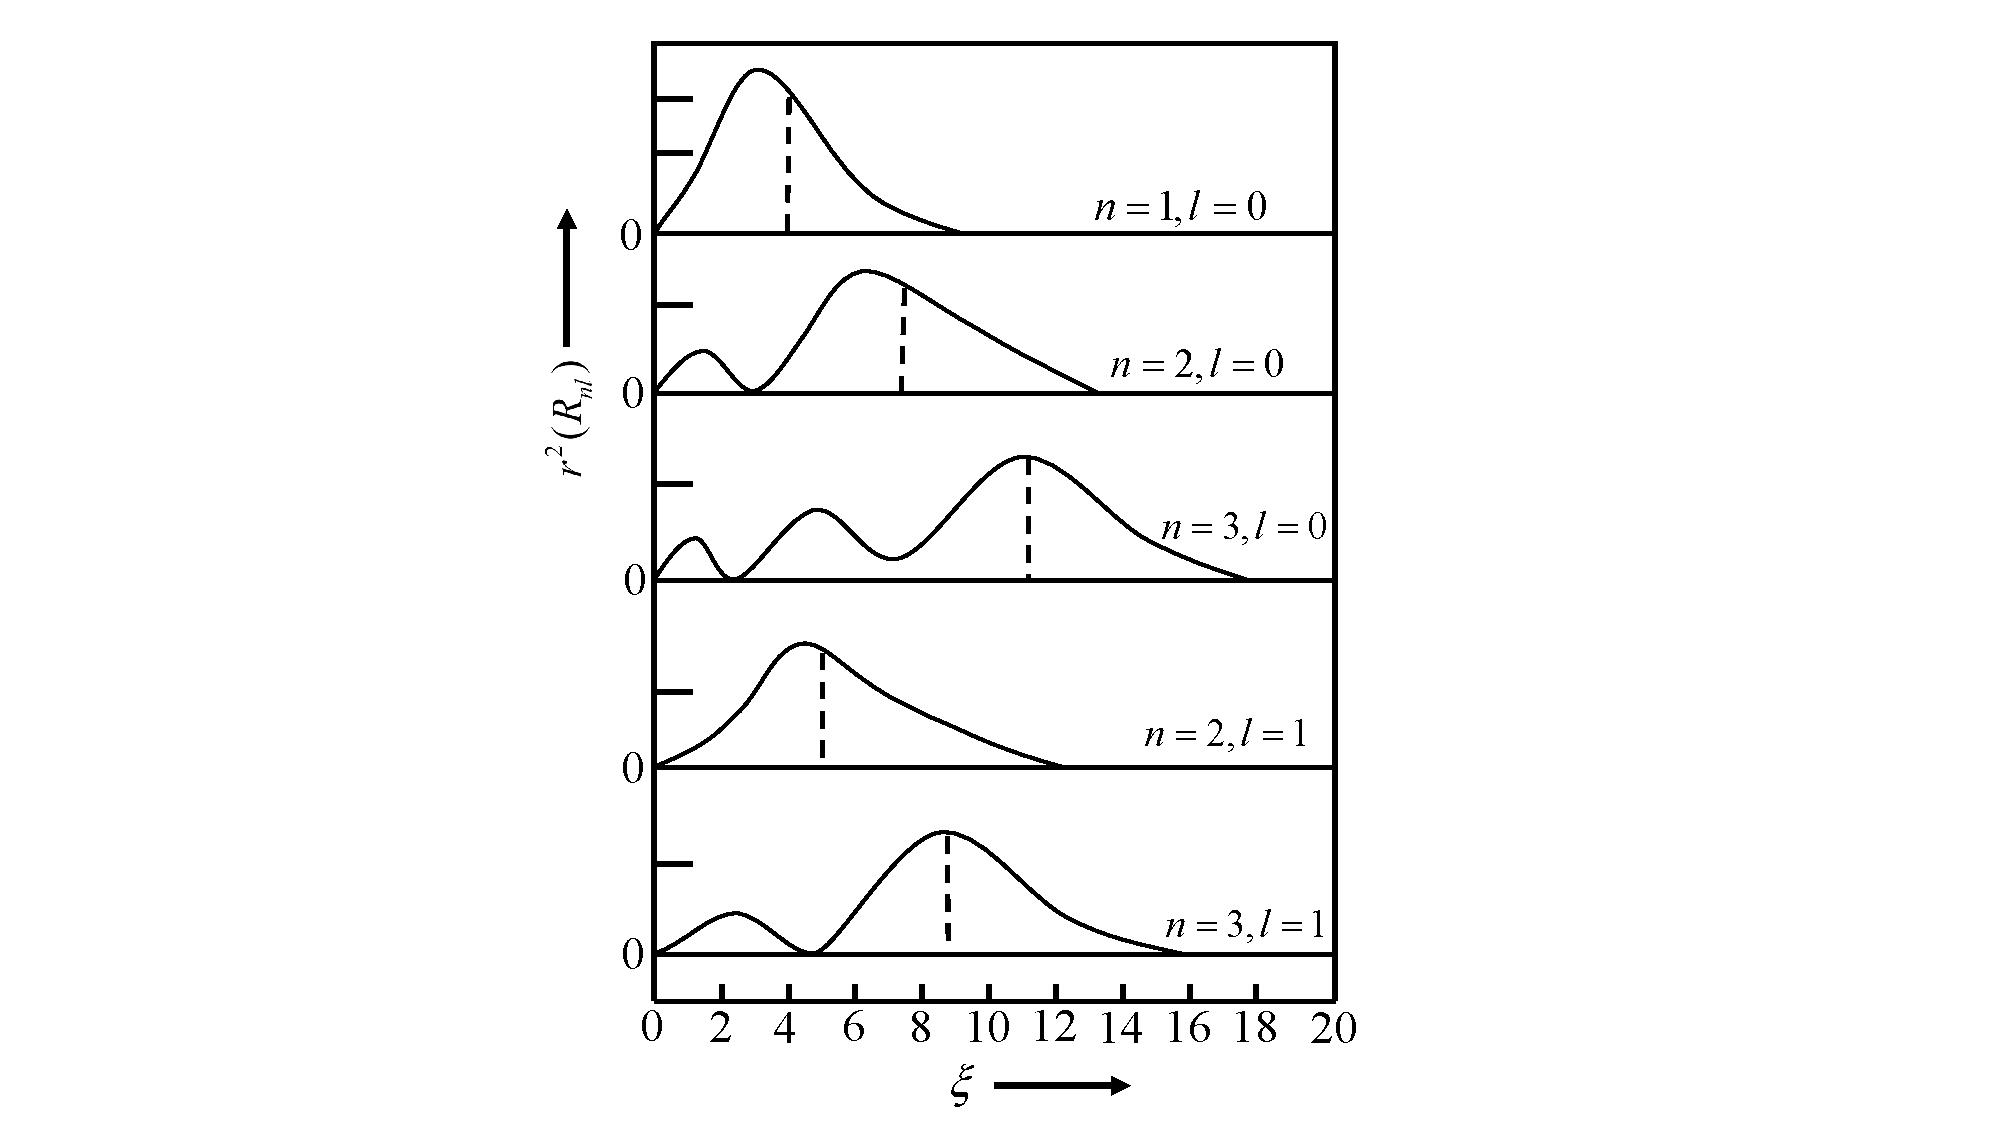
\includegraphics[width=5cm,clip]{QM file/figure/5-4}
	\caption{径向概率分布}\label{fig.5-4}
	\caption*{{\footnotesize 横坐标$\xi=\frac{2Zr}{na_{0}}$,虚线$\vdots$标出了$\bar{r}$的值.曲线的最高点所相应的$\xi$值即最概然半径}}
\end{figure}
在\eqref{eq54.3}式描述的状态下,任何$r$的函数(作为物理量)$G(r)$的平均值显然是
\begin{empheq}{equation}\label{eq54.36}
	\bar{G}=\int_{0}^{\infty}G(r)R^{2}r^{2}dr=\int_{0}^{\infty}G(r)u^{2}(r)dr
\end{empheq}
$\varPsi_{nlm}$态下电子的径向概率分布如图\ref{fig.5-4}所示.

{\heiti 角分布}

波函数$\varPsi_{nlm}$所反映的空间概率分布一般具有方向性.在任何一个球壳层内,电子在方向$(\theta,\varphi)$附近,立体角元$d\Omega=\sin\theta d\theta d\varphi$内出现概率比例于
\begin{empheq}{equation}\label{eq54.37}
	|Y_{lm}(\theta,\varphi)|^{2}d\Omega=A_{lm}^{2}|P_{l}^{m}(\cos\theta)|^{2}d\Omega
\end{empheq}
例如对于$l=1,m=1$的状态$\varPsi_{n11}$,由于$P_{1}^{1}=\sin\theta$,电子的角分布概率密度与$\sin^{2}\theta$成比例,电子出现概率最大的方向是$\theta
=\frac{\pi}{2}$,即$x-y$平面.s态$(l=0)$波函数$\varPsi_{n00}$与$\theta,\varphi$无关,电子的空间概率分布是各向同性的.

{\heiti 和玻尔量子论的比较}

以氢原子为例,将玻尔量子论的主要结果和量子力学结果作一比较.在玻尔量子论中,关于电子稳定轨道的计算同时应用了牛顿力学和量子化条件.根据牛顿力学,在库仑力作用下,电子的运动轨道是圆或椭圆,正电荷(原子核)位于圆心或椭圆的焦点.电子运动的能量$E$,轨道角动量$\boldsymbol{L}$,运行周期$\tau$和轨道的长半径$a$,短半径$b$(圆轨道$b=a$)之间有关系\footnote{钱伯初.行星轨道问题和玻尔量子论.大学物理.1985,6:7}
\begin{empheq}{align}	%38,39,40\label{eq54.3}
	E&=-\frac{e^{2}}{2a}		\label{eq54.38}\\
	\boldsymbol{L}^{2}=-2\mu& Eb^{2}=\frac{\mu e^{2}b^{2}}{a}		\label{eq54.39}\\
	\tau=\frac{2\pi\mu ab}{L},&\quad \tau^{2}=\frac{4\pi^{2}\mu a^{3}}{e^{2}}		\label{eq54.40}
\end{empheq}
量子化条件为
\begin{empheq}{equation}\label{eq54.41}
	L=n_{\varphi}\hbar,\quad n_{\varphi}=1,2,3,\cdots
\end{empheq}
由于能量$E$只和长半径$a$有关,当能量确定后,轨道的短半径仍有多种取值.角动量$\boldsymbol{L}$与短半径$b$成正比,而以圆轨道的角动量为最大.如以$n$表示圆轨道的角动量量子数$(\boldsymbol{L}=n\hbar)$,$a_{n}$表示其半径,$E_{n}$表示其能量,由\eqref{eq54.39}、\eqref{eq54.41}式易得
\begin{empheq}{equation}\label{eq54.42}
	a_{n}=\frac{n^{2}\hbar^{2}}{\mu e^{2}}=n^{2}a_{0},\quad n=1,2,\cdots
\end{empheq}
代入\eqref{eq54.38}式,得到能级
\begin{empheq}{equation}\label{eq54.43}
	E_{n}=-\frac{e^{2}}{2a_{n}}=-\frac{e^{2}}{2n^{2}a_{0}}
\end{empheq}
属于能级$E_{n}$的各种稳定轨道,长半径相同,均为$a_{n}$,角动量和短半径为
\begin{empheq}{align}	%44,45\label{eq54.4}
	L=n_{\varphi}\hbar,\quad n_{\varphi}&=n,n-1,\cdots,1		\label{eq54.44}\\
	b=\frac{n_{\varphi}}{n}a_{n}&=nn_{\varphi}a_{0}		\label{eq54.45}
\end{empheq}
总之,每一条稳定轨道的形状,由量子数$n,n_{\varphi}$标志,但能量仅与$n$有关.电子沿这样的稳定轨道运动时,等效的电流和磁矩为

\begin{empheq}{equation*}
	\text{电流}|I|=\frac{e}{\tau}=\frac{eL}{2\pi\mu ab}
\end{empheq}	\eqlong
\begin{empheq}{align}\label{eq54.46}
	\text{磁矩}|M|&=\frac{|I|}{c}\pi ab=\frac{eL}{2\mu c}	\nonumber\\
	&=n_{\varphi}\frac{e\hbar}{2\mu c}=n_{\varphi}\mu_{B}\quad\text{(高斯单位制)}
\end{empheq}\eqnormal
$\mu_{B}=\frac{e\hbar}{2\mu c}$为玻尔磁子.

如再考虑空间量子化(轨道法线的空间指向的量子化),还应该有
\begin{empheq}{align}	%47,48
	L_{z}=m\hbar,\quad m=0,&\pm1,\cdots,\pm n_{\varphi}		\label{eq54.47}\\
	M_{z}=-\frac{e}{2\mu c}L_{z}&=-m\mu_{B}		\label{eq54.48}
\end{empheq}

以上是玻尔量子论的主要结果,它和量子力学结果有相同之处,也有差异,列举如下:

(1) 能级公式,两种理论给出的结果相同.

(2) 就角量子数($l$或$n_{\varphi}$)与主量子数$n$的关系而言,$n_{\varphi}$相当于$(l+1)$.量子力学中$l$的最大值$l=(n-1)$所对应的状态相当于玻尔圆轨道.

(3) 就$L_{z}$的本征值而言,两种理论均给出
\begin{empheq}{equation*}
	L_{z}=m\hbar,\quad m=0,\pm1,\pm2,\cdots
\end{empheq}
但两种理论关于$\boldsymbol{L}^{2}$的本征值给出不同的结果,
\begin{empheq}{equation*}
	{\boldsymbol{L}^{2}=}
	\begin{dcases}
		n_{\varphi}^{2}\hbar^{2}	\quad\qquad\text{(玻尔量子论)}	\\
		l(l+1)\hbar^{2}	\quad \text{(量子力学)}
	\end{dcases}
\end{empheq}
当量子数较小时,两种结果有本质的差异,可以认为是不确定度关系起了重要作用.当量子数很大时,大致可以认为$n_{\varphi}$,相当于$\bigg(l+\frac{1}{2}\bigg)$.但就$L_{z}$的最大值而言,则$n_{\varphi}$相当于$l$.总之,$n_{\varphi}$和$l$的对应关系视着眼点之不同而稍有差异.

(4) 磁矩与角动量的关系,两种理论结果相同(量子力学理论见$\S$\ref{sec:05.01})但两种理论关于原子中由于电子运动而形成的电流分布,给出不同的结论.按照玻尔量子论,每一条稳定轨道相当于一个电流环(圆形或椭圆形).而量子力学结果($\S$\ref{sec:05.01})则是,当电子处于$\varPsi_{nlm}$态时,在空间任何地点,沿纬线方向均有电流存在.按照\eqref{eq51.28}式(取$q=-e$),
\begin{empheq}{equation*}
	j_{\varphi}=-m\frac{e\hbar}{\mu}\frac{\varPsi^{*}\varPsi}{r\sin\theta}
\end{empheq}
电流呈环状分布,以$z$轴为对称轴.

(5) 关于电子的空间位置,两种理论有着根本概念上的差异,在玻尔量子论中,电子的轨道是一条平面闭合曲线.如果是圆轨道,电子至原子核的相对距离是固定不变的.按照量子力学,在$\varPsi_{nlm}$态下,电子在全空间有一种概率分布.即使是$l$取最大值$(l=n-1)$的状态,电子仍可以在各种径向距离$(r)$上出现.但是,可以证明(习题5-11)对于$l=n-1$的状态,最概然半径等于$n^{2}a_{0}$,刚好等于玻尔圆轨道半径.

(6) 玻尔量子论中,不存在角动量$L=0$的稳定轨道.而在量子力学中,$l=0$的状态($s$态)常常是最重要的状态.能量最低的基态就是s态,由于$l=m=0$,波函数是实函数,电流和磁矩均等于0,而按照玻尔量子论,电子的基态轨道为圆形$(n=n_{\varphi}=1)$,等效磁矩等于$\mu_{B}$(玻尔磁子).实验已经判明,量子力学关于基态的结论$(l=m=0)$,磁矩为0,概率分布各向同性,等等)是正确的.

微妙的是,氢原子的基态$(nlm=100)$既是$l=0$的状态,又是$l$取最大值$(l=n-1=0)$的状态,在后一种意义上, 基态具有某些玻尔圆轨道的性质(如最概然半径刚好等于玻尔半径$a_{0}$),也就可以理解了.

{\heiti 物理模型}

由电荷异号的两个粒子(质量$m_{1},m_{2}$,电荷$q_{1},q_{2}$)构成的体系,如粒子间的作用主要是库仑作用,其他作用力可以忽略,则描述这两个粒子相对运动的哈密顿算符可以表示成
\begin{empheq}{equation}\label{eq54.49}
	\hat{H}=-\frac{\hbar^{2}}{2\mu}\nabla^{2}+\frac{q_{1}q_{2}}{r}\quad(q_{1}q_{2}<0)
\end{empheq}
其中$r$为相对坐标,$\mu=\frac{m_{1}m_{2}}{m_{1}+m_{2}}$是折合质量.与\eqref{eq54.2}式相比,相当于$Z\e^{2}$换成$|q_{1}q_{2}|$,$\mu$换成折合质量.所以,只要在波函数中也作相应的代换,本节的结果就可应用于这个二粒子体系。这样的体系有

氢原子-原子核为质子,电荷$q_{1}=+e$.电子电荷$q_{2}=-e$.

类氢离子-由原子核(电荷$q_{1}=Ze$)和一个电子构成,如$\ce{He}^{+},\ce{Li}^{++}$.

$\mu$原子-由原子核(电荷$q_{1}=Ze$)和一个$\mu$子(电荷$q_{2}=-e$)构成.$\mu$子质量为电子的207倍,其他性质与电子基本相同.

电子偶素-正、负电子$(e^{+},e^{-})$形成的束缚态.正电子$(e^{+})$是电子$(e^{-}$的反粒子,电荷$q_{1}=+e$,质量与电子相同.

还有一些问题,可以用本节的结果作为良好近似.例如,多电子原子(原子核电荷$Ze$)中的最内层($k$层)电子,所受作用力主要来自原子核,其状态很接近于由\eqref{eq54.30}式表示的基态$\varPsi_{100}$.又如,单价原子中最外层的价电子,所受作用势(原子核和内层电子库仑作用的总和)接近于$-\frac{\e^{2}}{r}$,价电子的波函数接近于氢原子的基态波函数$\varPsi_{100}$,但近似程度稍差.

\example 对于类氢离子的$\varPsi_{nlm}$态,计算离心势能的平均值.

\solution 径向方程\eqref{eq54.4}可以等效地看作一维定念薛定谔方程,能量算符相当于
\eqlong
\begin{empheq}{equation}\label{eq54.50}
	\hat{H}\Rightarrow-\frac{\hbar^{2}}{2\mu}\frac{d^{2}}{dr^{2}}+l(l+1)\frac{\hbar^{2}}{2\mu r^{2}}-\frac{Z\e^{2}}{r}=\hat{H}(l,r)
\end{empheq}\eqnormal
$u(r)$相当于波函数.视$l$为参数,则
\begin{empheq}{equation*}
	\frac{\partial\hat{H}}{\partial l}=(2l+1)\frac{\hbar^{2}}{2\mu r^{2}}
\end{empheq}
按照海尔曼定理($\S$\ref{sec:03.11}),应有
\begin{empheq}{equation}\label{eq54.51}
	\bigg\langle\frac{\partial\hat{H}}{\partial l}\bigg\rangle_{min}=\frac{\partial}{\partial l}E_{nlm}
\end{empheq}
今已知
\eqlong
\begin{empheq}{equation*}
	E_{nlm}=E_{n}=-\frac{1}{2n^{2}}\frac{\mu \e^{4}Z^{2}}{\hbar^{2}},\quad n=l+n_{r}+1
\end{empheq}
代入\eqref{eq54.51}式, 即得
\begin{empheq}{equation*}
	\frac{(2l+1)\hbar^{2}}{2\mu}\bigg\langle\frac{1}{r^{2}}\bigg\rangle_{min}=\frac{\partial E_{n}}{\partial l}=\frac{\partial E_{n}}{\partial n}=\frac{\mu \e^{4}Z^{2}}{n^{3}\hbar^{2}}
\end{empheq}\eqnormal
亦即
\begin{empheq}{equation}\label{eq54.52}
	\bigg\langle\frac{1}{r^{2}}\bigg\rangle_{min}=\frac{Z^{2}}{n^{3}\bigg(1+\frac{1}{2}\bigg)a_{0}^{2}}
\end{empheq}
离心势能平均值为
\eqlong
\begin{empheq}{equation}\label{eq54.53}
	\bigg\langle\frac{l(l+1)\hbar^{2}}{2\mu r^{2}}\bigg\rangle_{min}=\frac{l(l+1)Z^{2}\e^{2}}{(2l+1)n^{3}a_{0}}=-\frac{l(l+1)}{\bigg(l+\frac{1}{2}\bigg)n}
\end{empheq}\eqnormal
由于$(-E_{n})$等于动能平均值,所以在动能中离心势能所占比例为$\frac{l(l+1)}{\bigg(l+\frac{1}{2}\bigg)n}$.当$n$给定后,$l$越大,这个比例越大,当$l$取最大值$(n-1)$,这个比例为$\frac{n-1}{n-\frac{1}{2}}$,这时径向动能仅占动能的$\frac{1}{2n-1}$.所以,如$n\geqslant 1$,在$(n,n-1,m)$态中径向动能所占比例很小,这种状态相当于玻尔圆轨道.(牛顿力学中圆轨道$r$不变,径向动能为0.)

% 二维中心力场
\starthis\section[二维中心力场]{二维中心力场} \label{sec:05.05} % 
% \makebox[5em][s]{} % 短题目拉间距

在二维问题中,常用的坐标系有直角坐标$(x,y)$和平面极坐标$(\rho,\varphi)$,如图5 -5所示,它们的关系是
\begin{empheq}{align}
	x=\rho\cos\varphi,\quad y&=\rho\sin\varphi	\label{eq55.1}\\
	\rho=\sqrt{x^{2}+y^{2}},\quad \varphi&=\arctan\frac{y}{x}	\label{eq55.2}
\end{empheq}
粒子(质量$\mu$)受到二维中心力场作用时,势能$V$是径向距离$\rho$的函数,总能量算符可以表示成
\begin{empheq}{equation}\label{eq55.3}
	\hat{H}=\hat{T}+\hat{V}=-\frac{\hbar^{2}}{2\mu}\nabla^{2}+V(\rho)
\end{empheq}

\begin{wrapfigure}[8]{r}{6em}
	\centering
	\small
	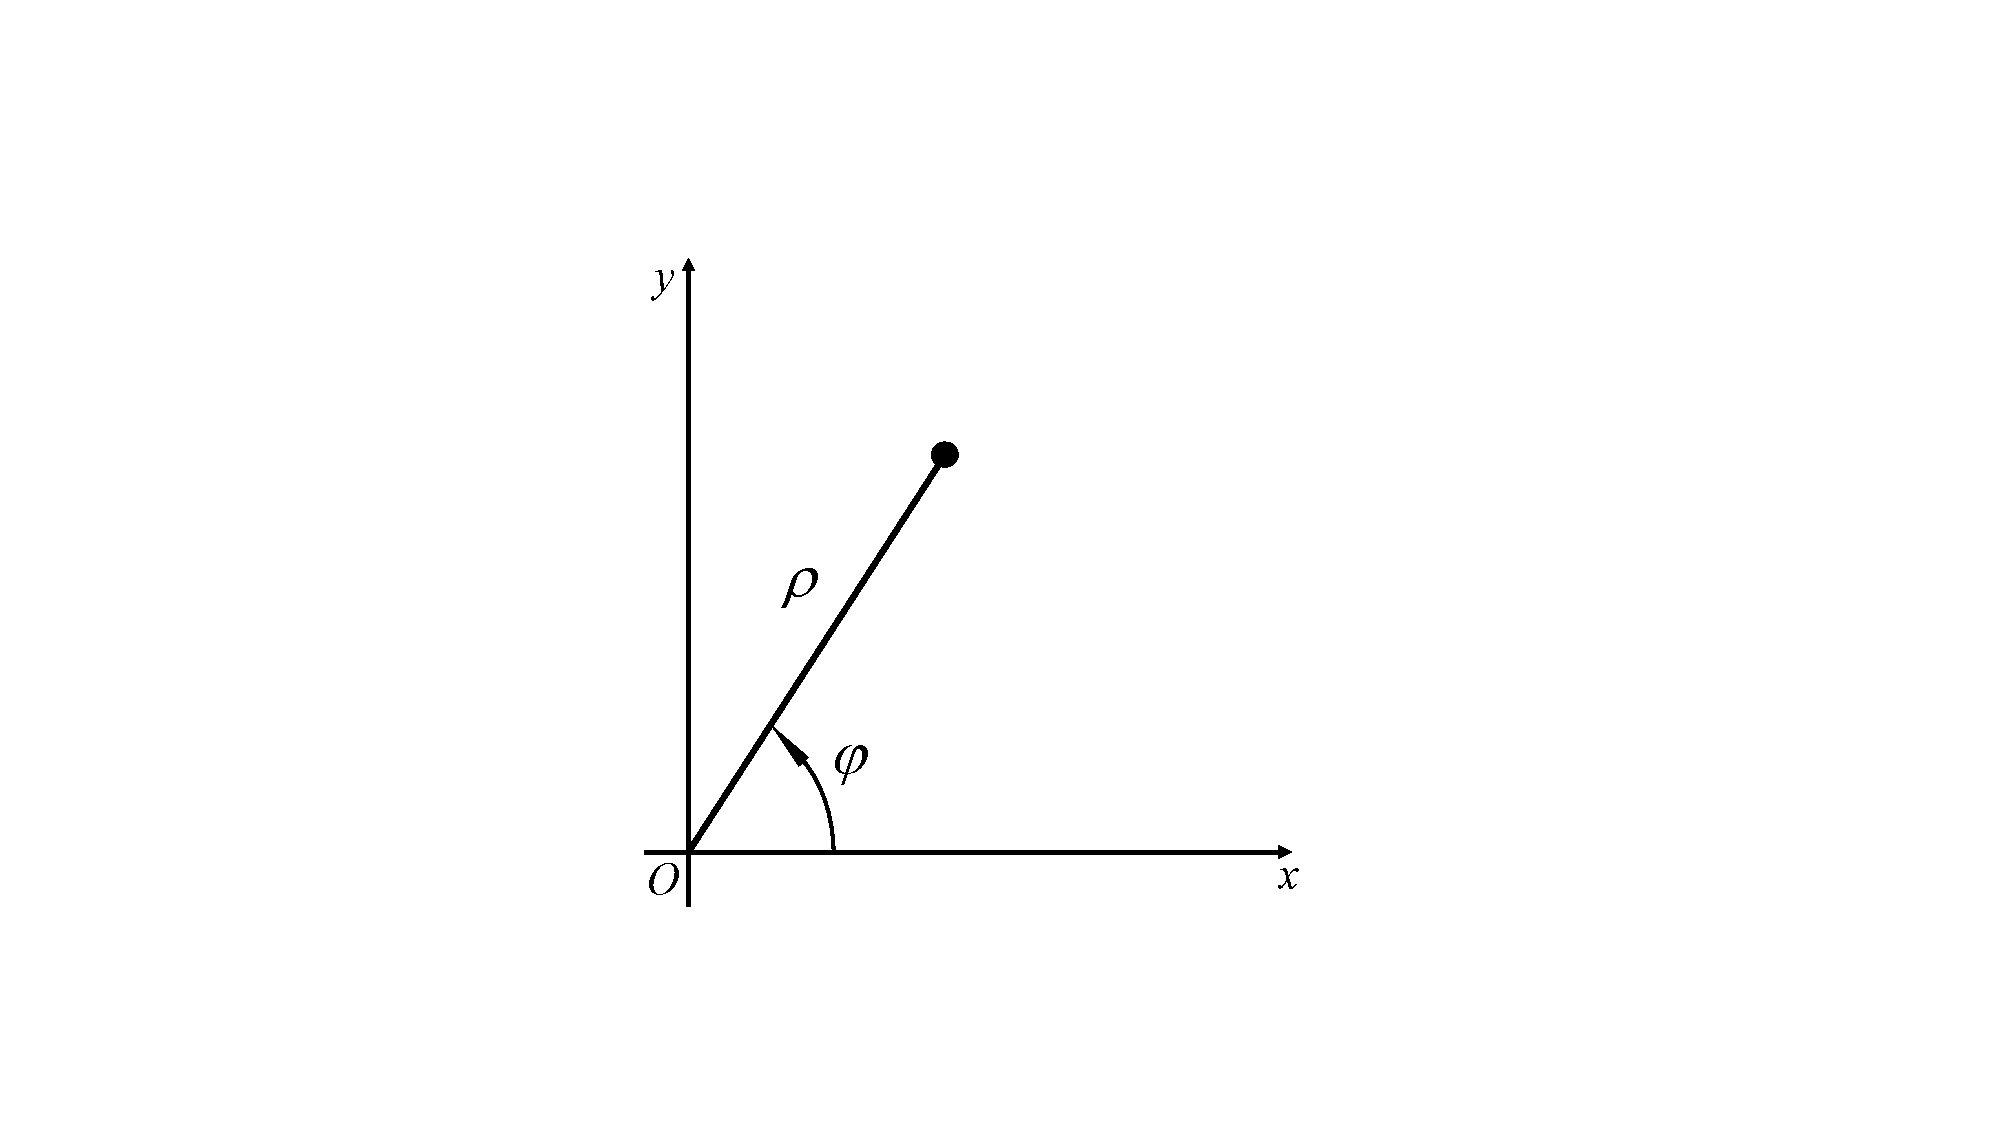
\includegraphics[width=2.5cm,clip]{QM file/figure/5-5}
	\caption{}\label{fig.5-5}
\end{wrapfigure}
\noindent 其中\eqllong
\begin{empheq}{align}\label{eq55.4}
	\nabla^{2}&=\frac{\partial^{2}}{\partial x^{2}}+\frac{\partial^{2}}{\partial y^{2}}	\nonumber\\
	&=\frac{\partial^{2}}{\partial \rho^{2}}+\frac{1}{\rho}\frac{\partial}{\partial \rho}+\frac{1}{\rho^{2}}\frac{\partial^{2}}{\partial \varphi^{2}}
\end{empheq}
角动量算符为
\begin{empheq}{equation}\label{eq55.5}
	\hat{L}_{z}=x\hat{p}_{y}-y\hat{p}_{x}=-i\hbar\frac{\partial}{\partial \varphi}
\end{empheq}\eqnormal
显然,$[\hat{L}_{z},\hat{H}]=0$,$\hat{L}_{z}$为守恒量.$\hat{H},\hat{L}_{z}$的共同本征函数可以表示成
\begin{empheq}{equation}\label{eq55.6}
	\psi(\rho,\varphi)=W(\rho)e^{im\varphi},\quad m=0,\pm1,\pm2,\cdots
\end{empheq}
$\hat{L}_{z}$的本征值为$m\hbar$.将\eqref{eq55.6}式代入能量本征方程
\eqshort
\begin{empheq}{equation}\label{eq55.7}
	\hat{H}\psi=E\psi
\end{empheq}\eqnormal
易得径向方程为
\eqllong
\begin{empheq}{equation}\label{eq55.8}
	\bigg[-\frac{\hbar^{2}}{2\mu}\bigg(\frac{d^{2}}{d\rho^{2}}+\frac{1}{\rho}\frac{d}{d\rho}\bigg)+\frac{m^{2}\hbar^{2}}{2\mu\rho^{2}}+V(\rho)\bigg]W(\rho)=EW(\rho)
\end{empheq}\eqnormal
方括号中第一项可以解释成径向动能算符,第二项为离心势能.令
\eqshort
\begin{empheq}{equation}\label{eq55.9}
	W(\rho)=\rho^{-\frac{1}{2}}v(\rho)
\end{empheq}\eqnormal
可得$v(\rho)$满足的方程为
\eqlong
\begin{empheq}{equation}\label{eq55.10}
	\bigg[-\frac{\hbar^{2}}{2\mu}\frac{d^{2}}{d\rho^{2}}+\bigg(m^{2}-\frac{1}{4}\bigg)\frac{\hbar^{2}}{2\mu\rho^{2}}+V(\rho)	\bigg]v(\rho)=Ev(\rho)
\end{empheq}\eqnormal
径向波函数及能级$E$原则上可从\eqref{eq55.8}式或\eqref{eq55.10}式解出.

\eqref{eq55.10}式的构造与三维中心力场的径向方程[\eqref{eq51.14}式]有着高度的相似性,其对应关系为
\eqindent{7}
\begin{empheq}{alignat=6}\label{eq55.11}
	\text{三维} &\quad r &\quad V(r) &\quad u(r) & l &&\quad E 	\nonumber\\
	\text{二维} &\quad \rho &\quad V(\rho) &\quad v(\rho) \quad |m|&-\frac{1}{2} &&\quad E 
\end{empheq}\eqnormal
因此,如已求得三维中心力问题的解,根据对应关系就可以写出二维中心力问题的解.反之亦然.就能级而言,在三维问题的能级公式中,将$l$换成$|m|-\frac{1}{2}$,就得到相应的二维问题能级公式.由于$l$只取正整数或0,而$|m|-\frac{1}{2}$则是半奇数,所以两种能级是不相同的.这一点和经典力学有着根本概念上的不同.在经典力学中,粒子在中心力场中运动时,其轨迹是一条平面曲线,因此,就轨道形状和能量而言,三维问题与二维问题的结果必然相同.

\example 求二维类氢离子的束缚态$(E<0)$能级.

\solution 二维类氢离子中,电子所受作用势为
\begin{empheq}{equation}\label{eq55.12}
	V(\rho)=-\frac{Z\e^{2}}{\rho}
\end{empheq}
按照上述一般理论,$\hat{H},\hat{L}_{z}$的共同本征函数可以写成
\begin{empheq}{equation}\label{eq55.13}
	\varPsi=\rho^{-1/2}v(\rho)e^{im\varphi},\quad m=0,\pm1,\pm2,\cdots
\end{empheq}
将三维类氢离子能级公式[\eqref{eq54.20}式]中$l$换成$|m|-\frac{1}{2}$,$n_{r}$改写成$n_{\rho}$(径向量子数),即得本题所求能级为
\eqlong
\begin{empheq}{equation}\label{eq55.14}
	E=\frac{Z^{2}\e^{2}}{2a_{0}\bigg(n_{\rho}+|m|+\frac{1}{2}\bigg)},\quad n_{\rho}=0,1,2,\cdots
\end{empheq}\eqnormal
其中$a_{0}=\dfrac{\hbar^{2}}{\mu \e^{2}}$(玻尔半径),就能级序列而言,相当于三维能级公式中$n\rightarrow\bigg(n-\frac{1}{2}\bigg)$.

\newpage





% 习题
\begin{exercises}
\exercise 限于$l=1$ $(\boldsymbol{L}^{2}=2\hbar^{2})$的情形,利用$Y_{lm}(m=1,0,-1)$具体函数形式,用坐标轮换$(x\rightarrow y,y\rightarrow z,z\rightarrow x)$法求$\boldsymbol{L}^{2},L_{x}$共同本征函数,表示成$Y_{lm}$的线性叠加.再求$\boldsymbol{L}^{2},L_{y}$共同本征函数.

\exercise 限于$l=1$的情形.利用上题结果验证:$L_{x}=0$的本征函数,$L_{y}=0$的本征函数以及$L_{z}=0$的本征函数$(Y_{10})$三者互相正交.你能否不依赖本征函数的具体函数形式而对此结果给予理论的证明?

[提示:利用升降算符方法,求$Y_{10}$态$L_{x}^{2}$及平均值,从而论证$Y_{10}$态下$L_{z}=0$的概率为0.]

\exercise 求$Y_{11}$态下$L_{x}$的可能测值及相应概率,用下述两种方法.

(a) 将$Y_{11}$按$\boldsymbol{L}^{2},L_{x}$,共同本征函数(5-1题)展开.

(b) 对$Y_{11}$态计算$L_{x}$及$L_{x}^{2}$平均值.

\exercise 设粒子状态为$\varPsi=A(x+y+2z)e^{-\lambda r}$,$(\lambda>0)$求

(a) $\boldsymbol{L}^{2}$的取值\quad(b)$\bar{L}_{z}$\quad(c)$L_{z}$等于$\hbar$的概率\quad(d)$L_{x}$的可能取值及相关概率.

\exercise 用不确定关系估算氢原子基态能量.

$\bigg[$提示:取$\Delta r\Delta p\sim\hbar,<r^{-1}>\sim\dfrac{1}{\Delta r}$$\bigg]$

\exercise 质量为$\mu$的粒子在中心力场$V(r)=-\lambda r^{-\frac{3}{2}}(\lambda>0)$中运动,试用不确定度关系估算基态能量.

\exercise 中心力问题的径向方程
\begin{empheq}{equation*}
	\bigg[-\frac{\hbar^{2}}{2\mu}\frac{d^{2}}{dr^{2}}+\frac{l(l+1)\hbar^{2}}{2\mu r^{2}}+V(r)\bigg]u(r)=Eu(r)
\end{empheq}
可以等效地当作一维能量本征方程,$u(r)$相当于波函数,等效能量算符为
\begin{empheq}{equation*}
	H(l,r)=-\frac{\hbar^{2}}{2\mu}\frac{d^{2}}{dr^{2}}+\frac{l(l+1)\hbar^{2}}{2\mu r^{2}}+V(r)
\end{empheq}
能级记为$E_{ln}(E_{l1}<E_{l2}<\cdots)$.试用海尔曼定理证明:$l$越大,$E_{ln}$越高($n$固定).

[提示:视$l$为参数,求$\partial H/\partial l$,再用海尔曼定理.]

\exercise 对于氢原子基态$\varPsi_{100}$,计算$\Delta x,\Delta p$,验证不确定度关系.

\exercise 对于氢原子基态$\varPsi_{100}$,计算电子出现在经典禁区的概率.

\exercise 对于氢原子的$(n,l,m)=(n,n-1,m)$态,计算电子出现在经典禁区的概率,并对$n=1,2,3,4,5$算出这个概率的数值,归纳出它对$n$的依赖关系.

\exercise 对于氢原子的$(n,n-1,m)$态,求最概然半径及$\bar{r}$,$\bar{r^{2}}$,$\Delta r$.

\exercise 原子核发生$\beta^{-}$衰变,电荷突然由$Ze$变成$(Z+1)e$.衰变过程中核外的电子波函数不受影响.对于原来处于原子$(Z)$的K层(1s层,$nlm=100$)的电子.衰变后仍旧处于原子$(Z+1)$的K层的概率等于多少?

\exercise 单价原子的外层电子(价电子)所受原子核及内层电子的平均作用势可以近似表示成
\begin{empheq}{equation*}
	V(r)=-\frac{\e^{2}}{r}-\lambda a_{0}\frac{\e^{2}}{r^{2}},\quad 0<\lambda \leqslant 1
\end{empheq}
试求价电子能级,与氢原子能级比较,列出主量子数$n$的修正数公式.

[提示:将$V(r)$的第二项与离心势能合并.]

\exercise 对于在中心力场$V(r)$中运动的粒子(质量$\mu$)的任何一个$(H,\boldsymbol{L}^{2},L_{z})$共同本征态,证明
\begin{empheq}{equation*}
	\bigg\langle\frac{dV}{dr}\bigg\rangle-\frac{l(l+1)\hbar^{2}}{\mu}\bigg\langle\frac{1}{r^{3}}\bigg\rangle=\frac{2\pi\hbar^{2}}{\mu}|\varPsi(0)|^{2}
\end{empheq}

$\bigg[$提示:将径向方程乘以$du$,再逐项积分.注意$r\rightarrow0,\infty$处的边界条件.也可先求$\bigg[H,\dfrac{\partial}{\partial r}\bigg]$,再对$\varPsi$计算平均值.$\bigg]$

\exercise 对于类氢离子(核电荷$Ze$)的$nlm$态,求$<r^{\nu}>,\nu=-1,-2,-3$.

$\bigg[$ 提示:利用海尔曼定理求出$\bigg\langle\dfrac{1}{r}\bigg\rangle$,$\bigg\langle\dfrac{1}{r^{2}}\bigg\rangle$,再利用上题证明的公式求$\bigg\langle\dfrac{1}{r^{3}}\bigg\rangle$.注意$l=0$时$\bigg\langle\dfrac{1}{r^{3}}\bigg\rangle\rightarrow\infty$ $\bigg]$.

\exercise 对于类氢离子(核电荷$Ze$)的$nlm$态,证明Kramers公式:
\eqindent{1}
\begin{empheq}{equation*}
	\frac{\lambda+1}{n^{2}}<r^{\lambda}>-(2\lambda+1)\frac{a_{0}}{Z}<r^{\lambda-1}>+\frac{\lambda}{4}[(2l+1)^{2}-\lambda^{2}]\frac{a_{0}^{2}}{Z^{2}}<r^{\lambda-2}>=0
\end{empheq}\eqnormal

求出公式成立的条件

[提示:以$r^{\lambda}u$乘径向方程,逐项积分.再以$2r^{\lambda+1}u^{\prime}$乘径向方程,逐项积分将两种结果合并,即可达到目的.]

\exercise 利用上题证明的公式,计算$nlm$态的$<r>,<r^{2}>$.

\exercise 对于氢原子的各s态$(nlm=nOO)$,计算$\Delta x,\Delta p_{x}$,并讨论经典极限$(n\geqslant1)$情况.

[提示:s态各向同性,$\overline{x^{2}}=\dfrac{1}{3}\overline{r^{2}},\overline{p_{z}^{2}}=\dfrac{1}{3}<\boldsymbol{p}^{2}>$.]

\exercise 类氢离子(核电荷$Ze$)$l\geqslant1$的情形下,按下列步骤对径向方程作近似处理:(a)求等效势能$V_{l}=V(r)+\dfrac{l(l+1)\hbar^{2}}{2\mu r^{2}}$极小值及相应距离$r_{l}$.(b)将$V_{l}$在$r_{l}$附近作泰勒展开,保留$(r-r_{l})^{2}$项.(c)视电子的径向运动为$r\sim r_{l}$附近的小振动,给定$l$,求最低能级与低激发能级,并和精确值比较.

\exercise 二维各向同性谐振子是指在势场
\begin{empheq}{equation*}
	V=\frac{1}{2}k(x^{2}+y^{2})=\frac{1}{2}\mu\omega^{2}\rho^{2},\quad \omega=\sqrt{\frac{k}{\mu}}
\end{empheq}
中运动的粒子.$\hat{H},\hat{L}_{z}$共同本征函数表示成$\varPsi=W(\rho)e^{im\varphi}$.写出$W(\rho)$满足的径向方程,并按下列步骤求解.

(a) 令$W(\rho)=u(\rho)\rho^{|m|}e^{-\alpha^{2}\rho^{2}/2}$,$\alpha=\sqrt{\dfrac{\mu\omega}{\hbar}}$

(b) 令$\dfrac{E}{\hbar\omega}=\varepsilon$,$\alpha^{2}\rho^{2}=\xi,u(\rho)=F(\xi)$,证明$F(\xi)$满足合流超几何方程.

(c) 仿照$\S$\ref{sec:05.04},论证$F(\xi)$必须是$n_{p}$次多项式.
 
(d) 确定能级.

\exercise 三维各向同性谐振子
\begin{empheq}{equation*}
	V=\frac{1}{2}k(x^{2}+y^{2}+z^{2})=\frac{1}{2}\mu\omega^{2}r^{2},\omega=\sqrt{\frac{k}{\mu}}
\end{empheq}

$H,\boldsymbol{L}^{2},L_{z}$共同本征函数表示成
\begin{empheq}{equation*}
	\varPsi=R(r)Y_{lm}(\theta,\varphi)=\frac{u(r)}{r}Y_{lm}(\theta,\varphi)
\end{empheq}

写出径向方程,并仿照上题方法求解.

[提示:令$u(r)=F(\xi)\xi^{(l+1)/2}e^{-\xi/2},\xi=\alpha^{2}r^{2}$.]

\exercise 讨论5-20,5-21题中能级的简并度,与2-15,2-16题的结果对照.

\exercise 对于三维各向同性谐振子的基态波函数,计算最概然半径,$\bar{r}$及$\Delta r$.

\exercise 仿照$\S$\ref{sec:05.04}例题所用方法,对于三维各向同性谐振子的$(n,lm)$态,计算离心势能$\dfrac{\boldsymbol{L}^{2}}{2\mu r^{2}}$的平均值.


\end{exercises}




% 第六章 定态微扰论与变分法
\chapter{定态微扰论与变分法}\label{chp:06}
% \makebox[5em][s]{} % 短题目拉间距

在量子力学中,薛定谔方程能够精确求解的情形不多,因此近似方法具有特殊的重要性.本章介绍处理定态问题的两种主要近似方法,即定态微扰论与变分法.半个多世纪以来,量子力学在应用方面已经有了许多进展,这些近似方法也有了许多发展、限于篇幅,我们只能对这些方法作初步介绍.

% 非简并态微扰论
\section[非简并态微扰论]{非简并态微扰论} \label{sec:06.01} % 
% \makebox[5em][s]{} % 短题目拉间距

研究一个物理体系,基本问题之一是求解能量本征方程
\begin{empheq}{equation}\label{eq61.1}
	\hat{H}\varPsi=E\varPsi
\end{empheq}
求出束缚态波函数和能级.如精确求解有困难,在下述前提下可以用微扰论方法求近似解.前提是:能量算符$\hat{H}$可以分解成大、小两项,
\begin{empheq}{equation}\label{eq61.2}
	\hat{H}=\hat{H}_{0}+\hat{H}^{\prime}
\end{empheq}
$\hat{H}_{0}$和$\hat{H}^{\prime}$均为厄密算符,按量级说$H^{\prime}\leqslant H_{0}$,而且$\hat{H}_{0}^{\prime}$的本征函数和本征值是已知的,或可以求出的.$H_{0}$称为零级能量(算符),$H^{\prime}$称为微扰.

$\hat{H}_{0}^{\prime}$的正交归一化本征函数记为$\varPsi_{k}^{(0)}$,$k=1,2,\cdots,n,\cdots$是编号数,与$\varPsi_{k}^{(0)}$相应的本征值记为$E_{k}^{(0)}$.$\varPsi_{k}^{(0)}$满足本征方程
\begin{empheq}{equation}\label{eq61.3}
	\hat{H}_{0}\varPsi_{k}^{(0)}=E_{k}^{(0)}\varPsi_{k}^{(0)}
\end{empheq}
及正交归一条件
\begin{empheq}{equation}\label{eq61.4}
	\langle \varPsi_{n}^{(0)}|\varPsi_{k}^{(0)} \rangle =\int\varPsi_{n}^{(0)*}\varPsi_{k}^{(0)}d\tau=\delta_{nk}
\end{empheq}
如果有几个本征函数相应于同一个能级$E_{k}^{(0)}$,这个能级称为简并能级,相应的那些本征态称为简并态.如果某个能级$E_{n}^{(0)}$只有一个相应的本征函数$\varPsi_{n}^{(0)}$,则称为非简并能级和非简并态.$\hat{H}_{0}$的全部本征态中,可能有一些是非简并态,其余则是简并态.例如氢原子(不考虑电子的自旋),基态$\varPsi_{100}$是非简并的,其他能量本征态$\varPsi_{nlm}(n\geqslant2)$都是简并态.在以下的叙述中,假定着重讨论的那个能级$(E_{n})$是非简并的.

回到\eqref{eq61.1}式的求解.由于$\hat{H}$中存在微扰$\hat{H}^{\prime}$,原来的($H_{0}$的)能级$E_{n}^{(0)}$将变成$E_{n}$,本征函数$\varPsi_{n}^{(0)}$将变成$\varPsi_{n}$,并满足\eqref{eq61.1}式,即
\begin{empheq}{equation*}\label{eq61.1'}
	(\hat{H}_{0}+\hat{H}^{\prime})\varPsi_{n}=E_{n}\varPsi_{n}
	\tag{$6.1.1^{\prime}$}
\end{empheq}
由于$H^{\prime}\leqslant H_{0}$,且与$E_{n}^{(0)}$将只有微小的差别,也与$\varPsi_{n}^{(0)}$也只有微小差别.为了求出$E_{n},\varPsi_{n}$,可设
\begin{empheq}{align}
	E_{n} &=E_{n}^{(0)}+E^{(1)}+E^{(2)}+\cdots	\label{eq61.5}\\
	\varPsi_{n} &=\varPsi_{n}^{(0)}+\varPsi^{(1)}+\varPsi^{(2)}	\label{eq61.6}
\end{empheq}
各项分别表示零级近似,一级修正,二级修正,等等,并规定各项的量级逐项相差$\frac{H^{\prime}}{H_{0}}$倍.关于\eqref{eq61.6}式,作如下规定.由于$\hat{H}_{0}$的全体本征函数$\{\varPsi_{k}^{(0)}\}$构成完备系,$\varPsi_{n}$可以展开成各$\varPsi_{k}^{(0)}$的线性叠加,
\begin{empheq}{equation*}
	\varPsi_{n}=\sum_{k}C_{k}\varPsi_{k}^{(0)}
\end{empheq}
暂不要求$\varPsi_{n}$是归一化的,则上式中总有一个系数(只要不为0)可以任意选择.为了方便,取$C_{n}=1$,则$\varPsi_{n}$的展开式为
\begin{empheq}{equation}\label{eq61.7}
	\varPsi_{n}=\varPsi_{n}^{(0)}+\sum_{k}^{\prime}C_{k}\varPsi_{k}^{(0)}
\end{empheq}
其中$\sum_{k}^{\prime}$表示对$k$求和,但$k\neq n$.这样做相当于规定\eqref{eq61.6}式中各个修正项中不含$\varPsi_{n}^{(0)}$项,因此这些修正项均与零级近似项正交,即
\begin{empheq}{equation}\label{eq61.8}
	\langle \varPsi_{n}^{(0)}|\varPsi^{(s)} \rangle =\int\varPsi_{n}^{(0)*}\varPsi^{(s)}d\tau=0,\quad s=1,2,\cdots
\end{empheq}
这个条件可以简化计算.将\eqref{eq61.5},\eqref{eq61.6}式代入\eqref{eq61.1'}式,并将各项按量级分开,可得:

\begin{subequations}\label{eq61.9}
	\eqindent{7}
	\begin{align}
	\shortintertext{零级项}
		(\hat{H}_{0}&-E_{n}^{(0)})\varPsi_{n}^{(0)}=0	\label{eq61.9a}\\
	\shortintertext{一级项}
		(\hat{H}_{0}-E_{n}^{(0)})&\varPsi^{(1)}=(E^{(1)}-\hat{H}^{\prime})\varPsi_{n}^{(0)}	\label{eq61.9b}\\
	\shortintertext{二级项}
		(\hat{H}_{0}-E_{n}^{(0)})\varPsi^{(2)}&=(E^{(1)}-\hat{H}^{\prime})\varPsi^{(1)}+E^{(2)}\varPsi_{n}^{(0)}	\label{eq61.9c}
	\end{align}\eqnormal
\end{subequations}
等等.\eqref{eq61.9a}式即\eqref{eq61.3}式$k=n$的情形.以$\varPsi_{n}^{(0)*}$左乘\eqref{eq61.9b}式,并对全空间积分,左端贡献为0,因此得到
\begin{empheq}{equation}\label{eq61.10}
	E^{(1)}=\int\varPsi_{n}^{(0)*}\hat{H}^{\prime}\varPsi_{n}^{(0)}d\tau=\langle \varPsi_{n}^{(0)}|\hat{H}^{\prime}|\varPsi_{n}^{(0)} \rangle \equiv H_{nn}^{\prime}
\end{empheq}
这就是能级$E_{n}$的一级修正项公式,$H_{nn}^{\prime}$的意义是微扰$H^{\prime}$在零级近似波函数$\varPsi_{n}^{(0)}$中的平均值对\eqref{eq61.9c}式作同样的处理,并注意到正交条件\eqref{eq61.8},可得
\begin{empheq}{equation}\label{eq61.11}
	E^{(2)}=\int\varPsi_{n}^{(0)*}\hat{H}^{\prime}\varPsi_{n}^{(1)}d\tau=\langle \varPsi_{n}^{(0)}|\hat{H}^{\prime}|\varPsi_{n}^{(1)} \rangle
\end{empheq}
但这还不是$E^{(2)}$的明显表示式,因为$\varPsi^{(1)}$尚未求出,设
\begin{empheq}{equation}\label{eq61.12}
	\varPsi^{(1)}=\sum_{k}^{\prime}C_{k}^{(1)}\varPsi_{k}^{(0)}
\end{empheq}
代入\eqref{eq61.9b}式,再用$\varPsi_{k}^{(0)*}$左乘全式,对全空间积分,并利用正交归一条件,可得
\begin{empheq}{equation}\label{eq61.13}
	C_{k}^{(1)}=\frac{H_{kn}^{\prime}}{E_{n}^{(0)}-E_{k}^{(0)}}
\end{empheq}
其中
\begin{empheq}{equation}\label{eq61.14}
	H_{kn}^{\prime}\equiv\int\varPsi_{k}^{(0)}\hat{H}^{\prime}\varPsi_{n}^{(0)}d\tau=\langle \varPsi_{k}^{(0)}|\hat{H}^{\prime}|\varPsi_{n}^{(0)} \rangle 
\end{empheq}
将\eqref{eq61.13}式代入\eqref{eq61.12}式,即得$\varPsi^{(1)}$的表示式
\begin{empheq}{equation}\label{eq61.15}
	\varPsi^{(1)}=\sum_{k}^{\prime}\frac{H_{kn}}{E_{n}^{(0)}-E_{k}^{(0)}}\varPsi_{k}^{(0)}
\end{empheq}
再代入\eqref{eq61.11}式, 即得
\begin{empheq}{equation}\label{eq61.16}
	E^{(2)}=\sum_{k}^{\prime}\frac{H_{nk}^{\prime}H_{kn}^{\prime}}{E_{n}^{(0)}-E_{k}^{(0)}}=\sum_{k}^{\prime}\frac{|H_{kn}^{\prime}|^{2}}{E_{n}^{(0)}-E_{k}^{(0)}}
\end{empheq}
用微扰论处理问题,通常的要求是,能级和波函数均应计算到第一个不等于零的修正项为止.对于波函数,由\eqref{eq61.15}式表示的一级修正总是不等于零的,一般不必再计算二级修正.对于能级,由于对称性等原因,$E^{(1)}$常常等于零,这时必须计算二级修正$E^{(2)}$.综合\eqref{eq61.5},\eqref{eq61.6},\eqref{eq61.10},\eqref{eq61.15},\eqref{eq61.16}式,可得准确到一级修正项的能量本征函数和准确到二级修正项的能级公式为
\eqlong
\begin{empheq}[box=\widefbox]{align}
	\varPsi_{n}&\approx\varPsi_{n}^{(0)}+\sum_{k}^{\prime}\frac{H_{kn}^{\prime}}{E_{n}^{(0)}-E_{k}^{(0)}}\varPsi_{k}^{(0)}		\label{eq61.17}	\\
	E_{n}&\approx E_{n}^{(0)}+H_{nn}^{\prime}+\sum_{k}^{\prime}\frac{|H_{kn}^{\prime}|^{2}}{E_{n}^{(0)}-E_{k}^{(0)}}		\label{eq61.18}
\end{empheq}\eqnormal


微扰论公式成立的条件为$|\varPsi^{(1)}|\leqslant|\varPsi_{n}^{(0)}|$,即
\begin{empheq}{equation}\label{eq61.19}
	|H_{kn}^{\prime}|\leqslant|E_{n}^{(0)}-E_{k}^{(0)}|,\quad k=1,2,\cdots
\end{empheq}
因此在能级密集的区域,微扰论的适用性稍差.

\example 一维谐振子,能量算符为
\begin{empheq}{equation*}
	H_{0}=-\frac{\hbar^{2}}{2m}\frac{d^{2}}{dx^{2}}+\frac{1}{2}m\omega^{2}x^{2}
\end{empheq}
设这谐振子受到微扰作用(另一种弹性力),
\begin{empheq}{equation*}
	H^{\prime}=\frac{\lambda}{2}m\omega^{2}x^{2},\quad |\lambda|\leqslant 1
\end{empheq}
试用微扰论公式计算能级的变化,并与精确解比较.

\solution $H_{0}$的本征函数记为$\varPsi_{n}^{(0)}$,这就是$\S$\ref{sec:02.05}讨论过的谐振子本征态.在表象中,(以$\varPsi_{n}^{(0)}$作为基矢)$x$的矩阵元只有下列类型不等于零:
\begin{empheq}{equation*}
	x_{n+1,n}=x_{n,n+1}=\bigg(\frac{n+1}{2}\frac{\hbar}{m\omega}\bigg)^{\frac{1}{2}}
\end{empheq}
因此,对于微扰$H^{\prime}$,它的矩阵元中不等于零的类型有
\begin{empheq}{align*}
	H_{nn}^{\prime} &=\frac{\lambda}{2}m\omega^{2}(x^{2})_{nn}=\frac{\lambda}{2}m\omega^{2}\sum_{k}x_{nk}x_{kn}	\\
	&=\frac{\lambda}{2}m\omega^{2}(|x_{n,n+1}|^{2}+|x_{n,n-1}|^{2})	\\
	&=\frac{1}{2}\bigg(n+\frac{1}{2}\bigg)\lambda\hbar\omega=\frac{\lambda}{2}E_{n}^{(0)}
	\\
	H_{n,n+2}^{\prime}&=H_{n+2,n}^{\prime}=\frac{\lambda}{2}m\omega^{2}x_{n,n+1}x_{n+1,n+2}	\\
	&=\frac{1}{4}\sqrt{(n+1)(n+2)}\lambda\hbar\omega
\end{empheq}
其中$E_{n}^{(0)}=\bigg(n+\frac{1}{2}\bigg)\hbar\omega$加是微扰前的能级.按照微扰论公式\eqref{eq61.10},\eqref{eq61.16}能级的一级修正和二级修正分别为
\begin{empheq}{align*}
	E_{n}^{1}&=H_{nn}^{\prime}=\frac{1}{2}\bigg(n+\frac{1}{2}\bigg)\lambda\hbar\omega	\\
	E_{n}^{(2)}&=\sum_{k}^{\prime}\frac{|H_{kn}^{\prime}|^{2}}{E_{n}^{(0)}-E_{k}^{(0)}}=\frac{1}{2\hbar\omega}(|H_{n-2,n}^{\prime}|^{2}-|H_{n+2,n}^{\prime}|^{2})	\\
	&=-\frac{1}{8}\bigg(n+\frac{1}{2}\bigg)\lambda^{2}\hbar\omega
\end{empheq}

本题显然可以精确求解,因为微扰后总能量算符为
\begin{empheq}{align*}
	H&=H_{0}+H^{\prime}=-\frac{\hbar^{2}}{2m}\frac{d^{2}}{dx^{2}}+\frac{1}{2}(1+\lambda)m\omega^{2}x^{2}	\\
	&=-\frac{\hbar^{2}}{2m}\frac{d^{2}}{dx^{2}}+\frac{1}{2}m\omega^{\prime2}x^{2},\quad \omega^{\prime}=\omega\sqrt{1+\lambda}
\end{empheq}
仍是谐振子问题.能级为
\begin{empheq}{equation*}
	E_{n}=\bigg(n+\frac{1}{2}\bigg)\hbar\omega^{\prime}=\bigg(n+\frac{1}{2}\bigg)\sqrt{1+\lambda}\hbar\omega
\end{empheq}
如将$\sqrt{1+\lambda}$展开成$\lambda$的幕级数,
\begin{empheq}{equation*}
	\sqrt{1+\lambda}=1+\frac{\lambda}{2}-\frac{\lambda^{2}}{8}+\cdots
\end{empheq}
则
\begin{empheq}{equation*}
	E_{n}=\bigg(n+\frac{1}{2}\bigg)\hbar\omega+\frac{\lambda}{2}\bigg(n+\frac{1}{2}\bigg)\hbar\omega-\frac{\lambda^{2}}{8}\bigg(n+\frac{1}{2}\bigg)\hbar\omega
\end{empheq}
准确到$\lambda^{2}$项,刚好和上述微扰论结果符合.







% 简并态微扰论
\section[简并态微扰论]{简并态微扰论} \label{sec:06.02} % 
% \makebox[5em][s]{} % 短题目拉间距

非简并态微扰论的特点是,受微扰作用后,原来的($\hat{H}_{0}$的)能级与本征函数都只发生微小的变化,$\varPsi_{n}^{(0)}\rightarrow\varPsi_{n}$,$E_{n}^{(0)}\rightarrow E_{n}$.简并态就不同,在微扰作用下,能级将发生分裂.

仍设$\hat{H}=\hat{H_{0}}+\hat{H}^{\prime}$,$\hat{H}^{\prime}$是微扰,设$\hat{H_{0}}$的某个能级$E_{n}^{(0)}$是$f$重简并的,有$f$个互相独立并且正交归一化的本征函数,
\begin{empheq}{equation}\label{eq62.1}
	\hat{H_{0}}\varPsi_{n\alpha}^{(0)}=E_{n}^{(0)}\varPsi_{n\alpha}^{(0)},\quad \alpha=1,2,\cdots,f
\end{empheq}
微扰$H^{\prime}$的存在一般地将引起这些本征态之间的耦合,因此,求解总能量的本征方程
\begin{empheq}{equation}\label{eq62.2}
	\hat{H}\varPsi_{n}=(\hat{H_{0}}+\hat{H}^{\prime})\varPsi_{n}=E_{n}\varPsi_{n}
\end{empheq}
时,$\varPsi_{n}$的零级近似一般应该是$\varPsi_{n\alpha}^{(0)}$的线性叠加,
\begin{empheq}{equation}\label{eq62.3}
	\varPsi_{n}^{(0)}=\sum_{\alpha}C_{\alpha}^{(0)}\varPsi_{n\alpha}^{(0)}
\end{empheq}
$\varPsi_{n}$的各级微扰修正仍记为$\varPsi^{(1)}$,$\varPsi^{(2)}$,$\cdots$,能级$E_{n}$的各级修正仍记为$E^{(1)}$,$E^{(2)}$,$\cdots$,即设
\begin{empheq}{align}
	\varPsi_{n}=\varPsi_{n}^{(0)}+\varPsi^{(1)}+\varPsi^{(2)}+\cdots	\label{eq62.4}\\
	E_{n}=E_{n}^{(0)}+E^{(1)}+E^{(2)}+\cdots		\label{eq62.5}
\end{empheq}
和上节一样,仍规定$\varPsi^{(1)}$,$\varPsi^{(2)}$,$\cdots$等不含$\varPsi_{n\alpha}^{(0)}$项,因此它们均和$\varPsi_{n\alpha}^{(0)}$正交,即
\begin{empheq}{align}\label{eq62.6}
	\langle \varPsi_{n\alpha}^{(0)}|\varPsi^{(1)} \rangle =0,\quad \langle \varPsi_{n\alpha}^{(0)}|\varPsi^{(2)} \rangle=0,\cdots
\end{empheq}
$\hat{H_{0}}$的其他($E_{n}^{(0)}$以外的)能级仍记为$E_{k}^{(0)}$,本征函数(不论是否简并)记为$\varPsi_{k}^{(0)}$
\begin{empheq}{equation}\label{eq62.7}
	\varPsi^{(1)}=\sum_{k}^{\prime}C_{k}^{(1)}\varPsi_{k}^{(0)}
\end{empheq}
将\eqref{eq62.4}、\eqref{eq62.5}式代入能量本征方程\eqref{eq62.2},并将各项按量级分开,形式上仍得到\eqref{eq61.9}列式,但必须牢记,现在由\eqref{eq61.3}式表示,它是$f$个简并态的线性叠加.

为了求出\eqref{eq62.3}式中各系数$C_{\alpha}^{(0)}$,以及能级的一级修正$E^{(1)}$,以各$\varPsi_{n\alpha}^{(0)*}(\alpha=1,2,\cdots,f)$轮流地左乘\eqref{eq61.9b}式,并对全空间积分,考虑到正交条件\eqref{eq62.6}式,即可得到下列关于$C_{\alpha}^{(0)}$的方程组:
\eqllong
\begin{empheq}{equation}\label{eq62.8}
	\begin{aligned}
		\begin{dcases}
			(H_{11}^{\prime}-E^{(1)})C_{1}^{(0)}+H_{12}^{\prime}C_{2}^{(0)}+\cdots+H_{1f}^{\prime}C_{f}^{(0)}=0	\\
			H_{21}^{\prime}C_{1}^{(0)}+(H_{22}^{\prime}-E^{(1)})C_{2}^{(0)}+\cdots+H_{2f}^{\prime}C_{f}^{(0)}=0	\\
			\qquad\qquad\qquad\quad\cdots\cdots\cdots\cdots	\\
			H_{f1}^{\prime}C_{1}^{(0)}+H_{f2}^{\prime}C_{2}^{(0)}+\cdots+(H_{ff}^{\prime}-E^{(1)})C_{f}^{(0)}=0
		\end{dcases}
	\end{aligned}
\end{empheq}\eqnormal
其中
\begin{empheq}{align}\label{eq62.9}
	H_{\alpha\beta}^{\prime}&\equiv H_{n\alpha,n\beta}=\int\varPsi_{n\alpha}^{(0)*}\hat{H}^{\prime}\varPsi_{n\beta}^{(0)}d\tau	\nonumber\\
	&=\langle \varPsi_{n\alpha}^{(0)}|\hat{H}^{\prime}|\varPsi_{n\beta}^{(0)} \rangle 
\end{empheq}
注意,\eqref{eq62.8}式中只出现$\{\varPsi_{n\alpha},\alpha=1,2,\cdots,f\}$子态矢空间中$\hat{H}^{\prime}$的矩阵元.实际上,\eqref{eq62.8}式相当于这子空间中微扰$\hat{H}^{\prime}$的本征方程,即
\eqlong
\begin{empheq}{equation*}\label{eq62.8'}
\begin{bmatrix}
	H_{11}^{\prime} & H_{12}^{\prime} & \cdots & H_{1f}^{\prime}	\\
	H_{21}^{\prime} & H_{22}^{\prime} & \cdots & H_{2f}^{\prime}	\\
	     \vdots     &      \vdots     &        & \vdots				\\
	H_{f1}^{\prime} & H_{f2}^{\prime} & \cdots & H_{ff}^{\prime}	\\
\end{bmatrix}\begin{bmatrix}
	C_{1}^{(0)}	\\	C_{2}^{(0)}	\\	\vdots	\\	C_{f}^{(0)}	\\
\end{bmatrix}=E^{(1)}\begin{bmatrix}
	C_{1}^{(0)}	\\	C_{2}^{(0)}	\\	\vdots	\\	C_{f}^{(0)}	\\
\end{bmatrix}
\end{empheq}
按照线性代数理论,\eqref{eq62.8}式存在非平庸解($C_{\alpha}^{(0)}$不全为0)的充要条件是
\begin{empheq}{equation}\label{eq62.10}
\begin{vmatrix}
	H_{11}^{\prime}-E^{(1)}	& H_{12}^{\prime} & \cdots & H_{1f}^{\prime}	\\
	H_{21}^{\prime}	& H_{22}^{\prime}--E^{(1)} & \cdots & H_{2f}^{\prime}	\\
	     \vdots     &      \vdots     &        & \vdots				\\
	H_{f1}^{\prime}	& H_{f2}^{\prime} & \cdots & H_{ff}^{\prime}-E^{(1)}	\\
\end{vmatrix}=0
\end{empheq}\eqnormal
亦即在$|\varPsi_{n\alpha}^{(0)}|$子空间中
\eqshort
\begin{empheq}{equation*}\label{eq62.10'}
	\det|H^{\prime}-E^{(1)}|=0
\end{empheq}
\eqref{eq62.10}式是$E^{(1)}$的$f$次代数方程,原则上可以求得$f$个$E^{(1)}$值,亦即原来的简并能级$E_{n}^{(0)}$在微扰论一级近似下已经分裂成为一组互相接近的能级.如\eqref{eq62.10}式的$f$个根互不重合,这表明在一级近似下能级$E_{n}^{(0)}$的简并化已经全部消除;如\eqref{eq62.10}式有重根,则表示简并化只是部分地消除.将由\eqref{eq62.10}式解出的每一个$E^{(1)}$值代回\eqref{eq62.8}式,求出$C_{\alpha}^{(0)}(\alpha=1,2,\cdots,f)$,并将其归一化,再代入\eqref{eq62.3}式,就得到和这个$E^{(1)}$相应的零级近似波函数.

有一种重要情况值得特别指出.如上述$f$个简并态中有一个特殊的$\varPsi_{n\beta}^{(0)}$,它与其他$\varPsi_{n\alpha}^{(0)}$构成的微扰矩阵元全部等于零,即$H_{\alpha\beta}^{\prime}=0$,则\eqref{eq62.8}式中唯一出现$C_{\beta}^{(0)}$的式子是
\begin{empheq}{equation*}
	(H_{\beta\beta}^{\prime}-E^{(1)})C_{\beta}^{(0)}=0
\end{empheq}\eqnormal
这时\eqref{eq62.8}式显然有特解
\begin{empheq}{equation*}
	E^{(1)}=H_{\beta\beta}^{\prime},\quad C_{\beta}^{(0)}=1,\quad C_{\alpha}^{(0)}=0(\alpha\neq\beta)
\end{empheq}
亦即$\varPsi_{n\beta}^{(0)}$单独构成正确的零级波函数,$E^{(1)}$等于微扰$H^{\prime}$的平均值.处理简并态微扰论问题,首先应该找出(如果有的话)这种特殊状态,问题就可得到简化.

波函数的一级修正$\varPsi^{(1)}$和能级的二级修正$E^{(2)}$也可以仿照$\S$\ref{sec:06.01}的程序而求出.$E^{(2)}$仍由\eqref{eq61.11}式表示,即
\eqlong
\begin{empheq}{equation}\label{eq62.11}
	E^{(2)}=\int\varPsi_{n}^{(0)*}\hat{H}^{\prime}\varPsi^{(1)}d\tau=\langle \varPsi_{n}^{(0)}|\hat{H}^{\prime}|\varPsi^{(1)} \rangle 
\end{empheq}\eqnormal
$\varPsi^{(1)}$由\eqref{eq62.7}式表示,$C_{k}^{1}$的公式仍可仿照$\S$\ref{sec:06.01}的程序求得,
\eqindent{1}
\begin{empheq}{equation}\label{eq62.12}
	C_{k}^{(1)}=\frac{\langle \varPsi_{k}^{(0)}|\hat{H}^{\prime}|\varPsi_{n}^{(0)} \rangle }{E_{n}^{(0)}-E_{k}^{(0)}}=\frac{1}{E_{n}^{(0)}-E_{k}^{(0)}}\sum_{\alpha}C_{\alpha}^{(0)}\langle \varPsi_{k}^{(0)}|\hat{H}^{\prime}|\varPsi_{n\alpha}^{(0)} \rangle 
\end{empheq}\eqnormal	\eqlong
\begin{empheq}{align}\label{eq62.13}
	\varPsi^{(1)}&=\sum_{n}^{\prime}\frac{1}{E_{n}^{(0)}-E_{k}^{(0)}}\langle \varPsi_{k}^{(0)}|\hat{H}^{\prime}|\varPsi_{n}^{(0)} \rangle\varPsi_{k}^{(0)}	\nonumber\\
	&=\sum_{k}^{\prime}\frac{\varPsi_{k}^{(0)}}{E_{n}^{(0)}-E_{k}^{(0)}}\sum_{\alpha}C_{\alpha}^{(0)}\langle \varPsi_{k}^{(0)}|\hat{H}^{\prime}|\varPsi_{n\alpha}^{(0)} \rangle
\end{empheq}
矩阵元$\langle \varPsi_{n}^{(0)}|\hat{H}^{\prime}|\varPsi_{n\alpha}^{(0)}\rangle$表示$\varPsi_{n\alpha}^{(0)}$态与$\varPsi_{k}^{(0)}$态由于$\hat{H}^{\prime}$的作用而产生耦合,因此(一级近似)波函数中出现$\varPsi_{k}^{(0)}$项.

将\eqref{eq62.13}式代入\eqref{eq62.11}式,即可得出$E^{(2)}$的具体表示式:
\begin{empheq}{align}\label{eq62.14}
	E^{(2)}&=\sum_{n}^{\prime}\frac{1}{E_{n}^{(0)}-E_{k}^{(0)}}\langle \varPsi_{n}^{(0)}|\hat{H}^{\prime}|\varPsi_{k}^{(0)} \rangle\langle \varPsi_{k}^{(0)}|\hat{H}^{\prime}|\varPsi_{n}^{(0)} \rangle	\\
	&=\sum_{k}^{\prime}\frac{1}{E_{n}^{(0)}-E_{k}^{(0)}}\sum_{\alpha,\beta}C_{\alpha}^{(0)}C_{\beta}^{(0)*}H_{n\beta,k}H_{k,n\alpha}	\nonumber	%\tag{$6.2.14^{\prime}$}
\end{empheq}
上式表明,能级的二级微扰修正$E^{(2)}$来源于微扰$H^{\prime}$引起的$\varPsi_{n}^{(0)}$态与其他各能级态$\varPsi_{k}^{(0)}$的耦合,矩阵元$\langle \varPsi_{k}^{(0)}|\hat{H}^{\prime}|\varPsi_{n}^{(0)}\rangle$就代表这种耦合.由于$\varPsi_{n}^{(0)}$系由$f$个简并态$\varPsi_{n\alpha}^{(0)},\varPsi_{n\beta}^{(0)},\cdots$组成,因此具体表现为下列形式的耦合:
\begin{empheq}{equation*}
	\varPsi_{n\alpha}^{(0)}\stackrel{H^{\prime}}{——}\varPsi_{k}^{(0)}\stackrel{H^{\prime}}{——}\varPsi_{n\beta},\quad \alpha,\beta=1,2,\cdots,f
\end{empheq}\eqnormal
而对于非简并能级,与$E_{n}^{(0)}$相应的状态只有一个$\varPsi_{n}^{(0)}$,二级能量修正$E_{n}^{(2)}$相应于耦合$\varPsi_{n}^{(0)}-\varPsi_{k}^{(0)}-\varPsi_{n}^{(0)}$,$E_{k}^{(0)}\neq E_{n}^{(0)}$.

处理简并态微扰论问题,核心目标是弄清楚能级的分裂情况.如在一级近似下,能级已经分裂,简并已经消除,[与此相应,各个零级波函数$\varPsi_{n}^{(0)}$也可经由\eqref{eq62.8}式确定下来]一般就不必再计算能级的二级修正和波函数的一级修正.[如有必要,可按\eqref{eq62.13}、\eqref{eq62.14}式计算.]如在能量一级近似下,简并并未完全消除,则对于仍然简并的那些能级,零级波函数实际上无法经由\eqref{eq62.8}式而确定下来,因此\eqref{eq62.13}、\eqref{eq62.14}式实际上无法使用.这种情况下,需要重新处理,$\varPsi_{n}^{(0)}$将与$E^{(2)}$(甚至$E^{(3)}$,$\cdots$)同时求出,亦即能级分裂发生在高级近似下.

\example 研究氢原子的第二个能级在外电场中引起的分裂,即史塔克效应.(计算能级的一级修正,不考虑电子自旋.)

\solution 以$E_{n}^{(0)}$和$\varPsi_{nlm}^{(0)}$表示孤立氢原子的能级和能量本征态($H_{0},\boldsymbol{L}^{2},L_{z}$的共同本征态).能级$E_{n}^{(0)}$的简并度是$n^{2}$,第二个能级$E_{2}U(0)$共有4个本征态,$nlm$值为
\begin{empheq}{equation*}
	nlm=200,210,211,21-1
\end{empheq}
$\varPsi_{nlm}^{(0)}$可以表示成(参看$\S$\ref{sec:05.01},$\S$\ref{sec:05.04})
\begin{empheq}{equation*}
	\varPsi_{nlm}^{(0)}=R_{nl}(r)Y_{lm}(\theta,\varphi)
\end{empheq}
与本题有关的径向波函数只有2种,$R_{21}$及$R_{20}$,$Y_{lm}$则有4种,它们是
\begin{empheq}{align*}
	Y_{00}&=\sqrt{\frac{1}{4\pi}}	\\
	Y_{10}&=\sqrt{\frac{3}{4\pi}}\cos\theta=\sqrt{\frac{3}{4\pi}}\frac{z}{r}	\\
	Y_{11}&=-\sqrt{\frac{3}{8\pi}}\sin\theta e^{i\varphi}=-\sqrt{\frac{3}{8\pi}}\frac{x+iy}{r}	\\
	Y_{1-1}&=\frac{3}{8\pi}\sin\theta e^{-i\varphi}
\end{empheq}

将氢原子置于电场$\mathscr{E}$中,以电场方向作为$z$轴,则电场对电子的作用势为
\begin{empheq}{equation}\label{eq62.15}
	H^{\prime}=e\mathscr{E}\cdot\boldsymbol{r}=e\mathscr{E}z=e\mathscr{E}r\cos\theta
\end{empheq}
如电场强度$\mathscr{E}$不超过$10^{6}$\si{V/cm},则$H^{\prime}$的数量级为
\begin{empheq}{equation*}
	H^{\prime}<(10^{6}\si{eV/cm})(10^{-8}\si{cm})=10^{-2}\si{eV}
\end{empheq}
而电子能级间距为几个电子伏,所以$H^{\prime}$可以当作微扰.

由于$\hat{H}^{\prime}$和$\hat{L_{z}}$对易,$\hat{H}^{\prime}$作用于$\varPsi_{nlm}^{(0)}$的结果,$\hat{L_{z}}$的取值$(m\hbar)$不变.由于$\hat{H}^{\prime}$是奇宇称,所以在任何$\varPsi_{nlm}^{(0)}$态下$H^{\prime}$的平均值为0.这样一来,在上述4个简并态组成的子空间中,凡和(211)及(21-1)态有关的$H^{\prime}$矩阵元全部为0,也就是说,在波函数的零级近似中,$H^{\prime}$的作用并不能使(211)、(21-1)态与其他简并态发生耦合,它们就是正确的零级波函数,而且不受$H^{\prime}$影响,能级不发生变化(一级近似).

在$n=2$的上述态矢空间中,仅有的不等于零的$H^{\prime}$矩阵元是
\begin{empheq}{align*}
	H_{200,210}^{\prime}&=H_{210,200}^{\prime}=e\mathscr{E}\int z\varPsi_{200}\varPsi_{210}d\tau	\\
	&=\frac{e\mathscr{E}}{\sqrt{3}}\int_{0}^{\infty}r^{3}R_{20}R_{21}dr
\end{empheq}
径向波函数的具体函数形式见\eqref{eq54.27}、\eqref{eq54.28}式,经过简单计算,得到
\begin{empheq}{equation}\label{eq62.16}
	H_{200,210}^{\prime}=H_{210,200}^{\prime}=-3e\mathscr{E}a_{0}
\end{empheq}
$a_{0}=\frac{\hbar^{2}}{\mu\e^{2}}$是玻尔半径.读者如能注意到$Y_{lm}$和$H^{\prime}$在直角坐标系中的对称性(奇偶性),当能对上述关于$H^{\prime}$矩阵元的讨论加深印象.

至此,初步结论是,在外电场作用下,4个简并态中(211)态和(21-1)态并不与其他态耦合,能级仍保持原来的值.(200)态和(210)态则产生耦合,这将导致能级分裂.将简并态微扰论用于这两个简并态,令
\begin{empheq}{equation}\label{eq62.17}
	\varPsi_{n}^{(0)}=C_{1}^{(0)}\varPsi_{200}^{(0)}+C_{2}^{(0)}\varPsi_{210}^{(0)}
\end{empheq}
\eqref{eq62.8}式具体表现为
\begin{empheq}{equation}\label{eq62.18}
	{}\begin{dcases}
		E^{(1)}C_{1}^{(0)}+3e\mathscr{E}a_{0}C_{2}^{(0)}=0	\\
		3e\mathscr{E}a_{0}C_{1}^{(0)}+E^{(1)}C_{2}^{(0)}
	  \end{dcases}
\end{empheq}
\eqref{eq62.10}式表现为
\begin{empheq}{equation}\label{eq62.19}
	(E^{(1)})^{2}-(3e\mathscr{E}a_{0})^{2}=0
\end{empheq}
解为
\eqshort
\begin{empheq}{equation*}
	E^{(1)}=\pm3e\mathscr{E}a_{0}
\end{empheq}\eqnormal
此即能级$E_{2}^{(0)}$的一级微扰分裂(一级史塔克效应).再由\eqref{eq62.18}式可求出$C_{1}^{(0)}$,$C_{2}^{(0)}$,结果为
\eqllong
\begin{empheq}{equation}\label{eq62.20}
	\begin{aligned}
		E^{(1)}&=3e\mathscr{E}a_{0},\quad C_{1}^{(0)}=-C_{2}^{(0)},\quad 
		\varPsi^{(0)}=\frac{1}{\sqrt{2}}(\varPsi_{200}^{(0)}-\varPsi_{210}^{(0)})	\\
		E^{(1)}&=-3e\mathscr{E}a_{0},\quad C_{1}^{(0)}=C_{2}^{(0)},\quad 
		\varPsi^{(0)}=\frac{1}{\sqrt{2}}(\varPsi_{200}^{(0)}+\varPsi_{210}^{(0)})
	\end{aligned}
\end{empheq}\eqnormal
能级分裂如图\ref{fig.6-1}所示.

\begin{figure}[!h]
	\centering
	\small
	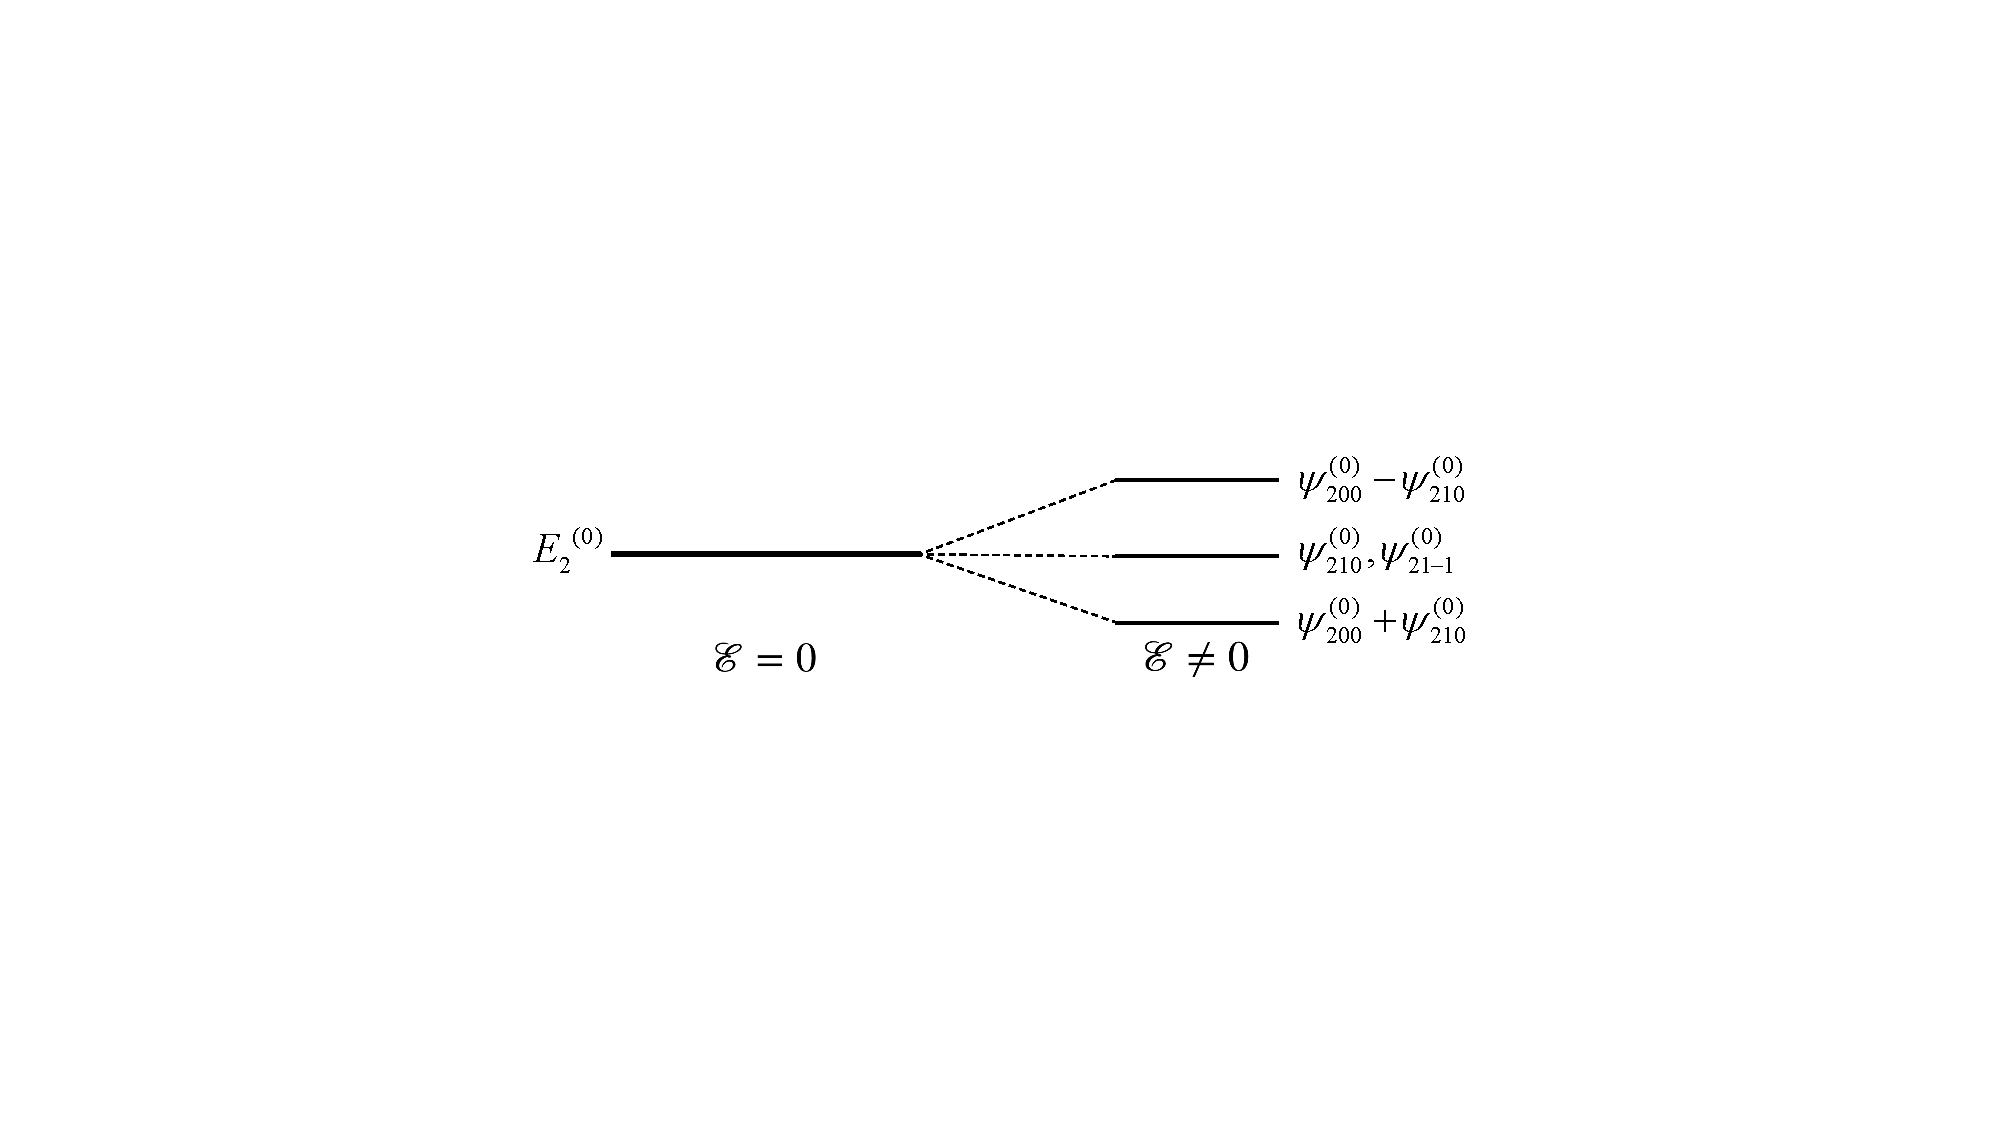
\includegraphics[width=6cm,clip]{QM file/figure/6-1}
	\caption{}\label{fig.6-1}
\end{figure}

值得注意的是原子的物理性质在外电场作用下发生的变化,氢原子的电偶极矩算符为
\eqshort
\begin{empheq}{equation}\label{eq62.21}
	\boldsymbol{D}=-e\boldsymbol{r}
\end{empheq}\eqnormal
未加电场时,原子的定态$\varPsi_{nlm}^{(0)}$均有或奇或偶的宇称,而$\boldsymbol{D}$为奇宇称,因此$\boldsymbol{D}$的平均值为0.在电场$\mathscr{E}$作用下,分裂出两个新的能级$E_{2}^{(0)}\pm3e\mathscr{E}a_{0}$,相应的波函数由\eqref{eq62.20}式表示,它们都是$\varPsi_{200}^{(0)}$和$\varPsi_{210}^{(0)}$的耦合态,已经没有宇称性,平均电矩也不为零,计算结果是
\eqlong
\begin{empheq}{align*}
	\varPsi^{(0)}&=\frac{1}{\sqrt{2}}(\varPsi_{200}^{(0)}-\varPsi_{210}^{(0)}),\quad \overline{D_{x}}=\overline{D_{y}}=0,\quad \overline{D_{z}}=-3ea_{0}	\\
	\varPsi^{(0)}&=\frac{1}{\sqrt{2}}(\varPsi_{200}^{(0)}+\varPsi_{210}^{(0)}),\quad \overline{D_{x}}=\overline{D_{y}}=0,\quad \overline{D_{z}}=3ea_{0}
\end{empheq}\eqnormal
正是耦合态的这个固有电矩在外电场中获得的势能
\begin{empheq}{equation*}
	E^{(1)}=0\langle \mathscr{E}\cdot\boldsymbol{D} \rangle=-\mathscr{E}\overline{D_{z}}=\pm3e\mathscr{E}a_{0}
\end{empheq}
造成了能级分裂.


% 变分法
\section[变分法]{变分法} \label{sec:06.03} % 
% \makebox[5em][s]{} % 短题目拉间距

考虑任一物理体系的束缚态,以$\hat{H}$表示体系的总能量算符($\hat{H}$与时间无关).任取一个归一化的波函数$\varPsi$(与时间无关),计算$\hat{H}$的平均值,并记为$E$,即
\begin{empheq}{align}
	&\int\varPsi^{*}\varPsi d\tau=\langle \varPsi|\varPsi \rangle =1		\label{eq63.1}\\
	E&=\int\varPsi^{*}\hat{H}\varPsi d\tau=\langle \varPsi|\hat{H}|\varPsi \rangle	\label{eq63.2}
\end{empheq}
然后令波函数作任意微小变化(变分)
\begin{empheq}{equation}\label{eq63.3}
	\varPsi\rightarrow\phi=\varPsi+\delta \varPsi
\end{empheq}
对于函数$\phi$重新计算$\hat{H}$的平均值,记为$E+\delta E$
\begin{empheq}{equation}\label{eq63.4}
	E+\delta E=\frac{\int\phi^{*}\hat{H}\phi d\tau}{\int\phi^{*}\phi d\tau}
\end{empheq}
(注意,$\phi$可能不再是归一化的)将\eqref{eq63.3}式代入\eqref{eq63.4}式,略去二级小量($\delta\varPsi$的二次项),得到如下结果:
\eqlong
\begin{empheq}{align*}
	\int\phi^{*}\phi d\tau &=1+\bigg(\int\varPsi\delta\varPsi^{*}d\tau+c.c \bigg)	\\
	\int\phi^{*}\hat{H}\phi d\tau&=\int(\varPsi^{*}+\delta\varPsi^{*})\hat{H}(\varPsi+\delta\varPsi)d\tau	\\
	&=E+\int\delta\varPsi^{*}\hat{H}\varPsi d\tau+\int\varPsi^{*}\hat{H}\delta\varPsi d\tau	\\
	&=E+\bigg(\int\delta\varPsi^{*}\hat{H}\varPsi d\tau+c.c \bigg)	\\
	&=E+\delta E+E\bigg(\int\varPsi\delta\varPsi^{*}d\tau+c.c\bigg)
\end{empheq}
即
\begin{empheq}{equation}\label{eq63.5}
	\delta E=\int\delta\varPsi^{*}\hat{H}\varPsi d\tau+c.c.-E\bigg(\int\delta\varPsi^{*}\varPsi d\tau+c.c \bigg)
\end{empheq}\eqnormal
考虑到$\delta\varPsi$的任意性,由\eqref{eq63.5}式容易看出以下结论:

(i) 如果$\varPsi$满足方程$\hat{H}\varPsi=E\varPsi$,则$\delta E=0$.

(ii) 如果对任意$\delta\varPsi$要求$\delta E=0$,则$\varPsi$必须满足
\eqshort
\begin{empheq}{equation}\label{eq63.6}
	\hat{H}\varPsi=E\varPsi
\end{empheq}\eqnormal
总之,“$\hat{H}$的平均值取变分极值$(\delta E=0)$”与“$\varPsi$为$\hat{H}$的本征函数”是等价的,这称为变分原理.

这个变分原理曾被薛定谔用来建立波动力学.本节向读者介绍一种寻找束缚态波函数与能级的近似方法,俗称变分法,它的理论基础就是上述变分原理.

设体系的总能量算符$\hat{H}$已经给定,但能量本征方程无法精确求解.设能级(按照由低到高的次序)为$E_{0},E_{1},E_{2},\cdots$相应的束缚态波函数(归一化的)为$\varPsi_{0}$,$\varPsi_{1}$,$\varPsi_{2}$,$\cdots$.任取一个归一化的波函数$\varPsi$,按照态叠加原理,$\varPsi$在原则上可以表示成能量本征函数的线性叠加:
\begin{empheq}{equation}\label{eq63.7}
	\varPsi=\sum_{n}C_{n}\varPsi_{n},\quad \sum_{n}C_{n}^{*}C_{n}=1
\end{empheq}
则在$\varPsi$态中$\hat{H}$的平均值(记为$E$)为
\begin{empheq}{equation}\label{eq63.8}
	E=\int\varPsi^{*}\hat{H}\varPsi d\tau=\sum_{n}C_{n}^{*}C_{n}E_{n}
\end{empheq}
由于$E_{n}\geqslant E_{0}$,显然$E\geqslant E_{0}$,$E_{0}$为基态能级.以上分析提示我们可以这样来寻找基态$\varPsi_{0}$,$E_{0}$.选取一种估计接近于基态的函数(归一化的)形式$\varPsi(\lambda,x)$,$x$代表坐标变量,$\lambda$为待定参数(一个或多个).对$\varPsi(\lambda,x)$计算$\hat{H}$的平均值,记为$E(\lambda)$,即
\begin{empheq}{equation}\label{eq63.9}
	E(\lambda)=\int\varPsi^{*}(\lambda,x)\hat{H}\varPsi(\lambda,x)d\tau
\end{empheq}
在不改变$\varPsi$的函数形式的条件下,根据变分极值条件
\begin{empheq}{equation}\label{eq63.10}
	\delta E=0,\quad \text{即}\frac{\partial E(\lambda)}{\partial\lambda}=0
\end{empheq}
求出$\lambda$的最佳值$\lambda_{0}$,相应的$\varPsi(\lambda_{0},x)$及$E(\lambda_{0}$即可作为基态波函数$\varPsi_{0}$及基态能级$E_{0}$的近似.如所得结果不够满意,可以另选一种$\varPsi$的函数形式,重复上述计算.在选择试探波函数$\varPsi(\lambda,x)$的函数形式时,当然应充分考虑基态的各方面性质,并可将其他近似方法(例如微扰论)求得的结果作为参考.一般说来,用这种参数变分法通常总能求得较好的结果,当然,计算工作量有时较大,需要电子计算机的帮助.

同样的方法也可用来寻找激发态$\varPsi_{n}$,$E_{n}$的近似,条件是所有能量小于$E_{n}$的能量本征态($\varPsi_{0}$,$\varPsi_{1}$,$\cdots$,$\varPsi_{n-1}$)均已求出,这时$\varPsi_{n}$的试探函数$\varPsi(\lambda,x)$应选取成与这些波函数正交,以保证在展开式\eqref{eq63.7}中没有这些状态的成分,则
\eqindent{7}
\begin{empheq}{align*}
	\varPsi&(\lambda,x)=C_{n}\varPsi_{n}+C_{n+1}\varPsi_{n+1}+\cdots	\\
	E(\lambda)&=C_{n}^{*}C_{n}E_{n}+C_{n+1}^{*}C_{n+1}E_{n+1}+\cdots\geqslant E_{n}
\end{empheq}\eqnormal
再用变分极值条件\eqref{eq63.10}式求出$\lambda$的最佳值$\lambda_{0}$,即可得到$\varPsi_{n}$,$E_{n}$的近似结果.

\example 粒子(质量$m$)在无限深势阱$(-a<x<a)$中运动.试用多项式近似结合变分法求基态能级的近似值,并与精确解比较.

\solution 精确解见$\S$\ref{sec:02.04},基态为(用本节的符号)
\begin{empheq}{equation}\label{eq63.11}
	\varPsi_{0}(x)=\sqrt{\frac{1}{a}}\cos\frac{\pi x}{2a},\quad E_{0}=\frac{\pi^{2}\hbar^{2}}{8ma^{2}}
\end{empheq}
$\varPsi_{0}$为偶宇称,并满足边界条件$\varPsi(a)=\varPsi(-a)=0$.

如用多项式作为$\varPsi_{0}$的近似表示,考虑到此为偶宇称,应取
\begin{empheq}{equation}\label{eq63.12}
	\varPsi=C_{0}+C_{2}\bigg(\frac{x}{a}\bigg)^{2}+C_{4}\bigg(\frac{x}{a}\bigg)^{4}+\cdots
\end{empheq}
如只取前两项,为了满足边界条件,必须取$C_{2}=-C_{0}$,而$C_{0}$可由归一化条件
\eqshort
\begin{empheq}{equation*}
	\int_{-a}^{a}\varPsi^{*}\varPsi dx=1
\end{empheq}
定出,结果为
\begin{empheq}{equation}\label{eq63.13}
	\varPsi=\sqrt{\frac{15}{16a}}\bigg(1-\frac{x^{2}}{a^{2}}\bigg)
\end{empheq}\eqnormal
这样已经不再有安插变分参数的余地.由\eqref{eq63.13}式求得能量平均值为
\eqlong
\begin{empheq}{equation}\label{eq63.14}
	E=\int_{-a}^{a}\varPsi^{*}\bigg(-\frac{\hbar^{2}}{2m}\frac{d^{2}}{dx^{2}}\bigg)\varPsi dx=\frac{5}{4}\frac{\hbar^{2}}{ma^{2}}
\end{empheq}\eqnormal
这和$E_{0}$的精确值已经相当接近,事实上
\begin{empheq}{equation*}
	E/E_{0}=10/\pi^{2}\approx\num{1.0132}
\end{empheq}

如取\eqref{eq63.12}式中前三项作为基态试探波函数,为了满足边界条件,应取$C_{4}=-(C_{0}+C_{2})$.如以$C_{0}$作为归一化系数,则试探波函数可以表示成
\eqlong
\begin{empheq}{equation}\label{eq63.15}
	\varPsi(\lambda,x)=C_{0}\bigg[1+\lambda\bigg(\frac{x}{a}\bigg)^{2}-(1+\lambda)\bigg(\frac{x}{a}\bigg)^{4}\bigg]
\end{empheq}\eqnormal
由归一化条件求出
\begin{empheq}{equation}\label{eq63.16}
	\frac{16}{315}(\lambda^{2}+8\lambda+28)aC_{0}^{2}=1
\end{empheq}
而能量平均值为
\eqlong
\begin{empheq}{align}\label{eq63.17}
	E(\lambda)&=-\frac{\hbar^{2}}{2m}\int_{-a}^{a}\varPsi(\lambda,x)\frac{d^{2}}{dx^{2}}\varPsi(\lambda,x)dx	\nonumber\\
	&=\frac{3}{4}\frac{11\lambda^{2}+36\lambda+60}{\lambda^{2}+8\lambda+28}\frac{\hbar^{2}}{ma^{2}}
\end{empheq}\eqnormal
根据变分极值条件\eqref{eq63.10}式,求得$\lambda$的最佳值为
\begin{empheq}{equation*}
	\lambda_{0}=-\num{1.22075},\quad \lambda_{0}^{\prime}=-\num{8.31775}
\end{empheq}
代入\eqref{eq63.17}式,得到
\eqlong
\begin{empheq}{equation}\label{eq63.18}
	E(\lambda_{0})=\num{1.23372}\frac{\hbar^{2}}{ma^{2}},\quad E(\lambda_{0}^{\prime})=\num{12.7663}\frac{\hbar^{2}}{ma^{2}}
\end{empheq}\eqnormal
$E(\lambda_{0})$和基态能级的精确值非常接近,事实上
\begin{empheq}{equation*}
	E_{0}=\frac{\pi^{2}}{8}\frac{\hbar^{2}}{ma^{2}}\approx \num{1.23370}\frac{\hbar^{2}}{ma^{2}}
\end{empheq}
\pskip
$E(\lambda_{0}^{\prime})$则接近于第三个能级$\frac{9\pi^{2}\hbar^{2}}{8ma^{2}}$.

将$\lambda_{0}=-\num{1.22075}$代入\eqref{eq63.15}式,所得波函数$\varPsi(\lambda_{0},x)$的波形非常接近于真正的基态$\varPsi_{0}$,计算表明
\begin{empheq}{equation*}
	\int_{-a}^{a}\varPsi_{0}\varPsi(\lambda_{0},x)dx=1-\alpha,\quad \alpha<10^{-5}
\end{empheq}
亦即$\varPsi(\lambda_{0},x)$中基态为主要成分,各种激发态成分之和仅为
\begin{empheq}{equation*}
	1-(1-\alpha)^{2}=2\alpha-\alpha^{2}\sim 10^{-5}.
\end{empheq}












% 习题
\begin{exercises}
	
\exercise 某物理体系只有两个能级.$H_{0}$在表象中$H$的矩阵表示为
\begin{empheq}{equation*}
	H=H_{0}+H^{\prime}=\begin{bmatrix}
		E_{1}^{(0)}+a & b \\
		b E_{2}^{(0)}+a	\\
	\end{bmatrix}
\end{empheq}
$a,b$为实数,并且远小于$(E_{2}^{(0)}-E_{1}^{(0)})$.试求能级的精确值.再按照微扰论公式写出能级(二级近似).比较两种结果.

\exercise 粒子在势阱
\begin{empheq}{equation*}
	{V(x)=}
	\begin{dcases}
		V_{0}x/a,\quad 0<x<a	\\
		\infty,\qquad x\leqslant0,x\geqslant a
	\end{dcases}
\end{empheq}
中运动,$V_{0}\leqslant\dfrac{\hbar^{2}}{m^{2}a}$,试用微扰论计算其能谱(一级近似).

[提示:利用无限深平底势阱(2-5题)的结果.]

\exercise 粒子在无限深势阱$(-a<x<a)$中运动.如受到微扰$H^{\prime}=\gamma\delta(x)$作用,求各能级产生的变化(一级修正).微扰论成立的条件是什么?

\exercise 三维自由转子的能量算符为$H_{0}=\dfrac{\boldsymbol{L}^{2}}{2\boldsymbol{I}}$,$\boldsymbol{I}$为转动惯量.试确定其能级及简并度.设此转子受到微扰$H^{\prime}=\lambda\cos\theta$作用,求基态能级的变化(二级近似).

\exercise 一维谐振子,受到微扰$H^{\prime}=\dfrac{\lambda p}{m}$作用,试按照微扰论公式求能谱(准确到$\lambda^{2}$),与精确值(3-30题)比较.

\exercise 三维各向同性谐振子,受到微扰
\begin{empheq}{equation*}
	H^{\prime}=\lambda xyz+\bigg(\frac{\lambda^{2}}{\hbar\omega}\bigg)x^{2}y^{2}z^{2}
\end{empheq}
作用,求基态能级,准确到$\lambda^{2}$.

[提示:采用直角坐标系,$\varPsi_{n_{1}n_{2}n_{3}}=\varPsi_{n1}(x)+\varPsi_{n2}(y)+\varPsi_{n3}(z)$].

\exercise 在类氢离子(核电荷$Ze$)的能谱计算中,通常视原子核为点电荷.这样求出的能级记成$E_{n}^{(0)}$.实际上原子核更接近于电荷均匀分布的小球,核半径$R=r_{0}Z^{1/3},r_{0}=\num{1.635}\times10^{-13}\si{cm}$.试求这种核电荷分布效应对于离子中电子基态能级的影响(一级微扰修正).

$\bigg[$提示:电子所受库仑作用势为
\begin{empheq}{equation*}
	{V(r)}
	\begin{dcases}
		-\frac{Z\e^{2}}{R}\bigg(\frac{3}{2}-\frac{r^{2}}{2R^{2}}\bigg),\quad r<R	\\
		-\frac{Z\e^{2}}{r},\qquad\quad \qquad\quad  r>R
	\end{dcases}
\end{empheq}
以$H^{\prime}=V(r)-\bigg(-\dfrac{Z\e^{2}}{r}\bigg)$作为微扰.注意$R\ll\dfrac{a_{0}}{Z}$.
$\bigg]$
\exercise 在静电场中,如点电荷获得的静电势能是$V(\boldsymbol{r})$,则将点电荷换成电荷均匀分布的小球(半径$r_{0}$)时,静电势能是
\begin{empheq}{equation*}
	U(\boldsymbol{r})=V(\boldsymbol{r})+\frac{1}{6}r_{0}^{2}\nabla^{2}V(\boldsymbol{r})+\cdots
\end{empheq}
其中$\boldsymbol{r}$为球心位置对于氢原子,(原子核即质子,视为点电荷)视电子为点电核时,库仑势能为$V(\boldsymbol{r})=-\dfrac{\ell^{2}}{r}$.如视电子为电荷均匀分布的小球,$r_{0}=\dfrac{\e^{2}}{m_{e}C^{2}}$(经典电子半径),库仑势能改为上述$U(\boldsymbol{r})$,求1s和2p能级的一级微扰修正.[相当于兰姆移位(Lamb shift)]

[提示:$H^{\prime}=V-V,\nabla^{2}\dfrac{1}{r}=-4\pi\delta(\boldsymbol{r})$]

\exercise 有一个在磁场中的三维转子,能量算符为
\begin{empheq}{equation*}
	H=k\boldsymbol{L}^{2}+\omega L_{z}+\lambda L_{x},\quad k,\omega\gg\lambda
\end{empheq}

(a) 视$\lambda$项为微扰,求能级的零级近似、一级修正、二级修正.

(b) 求能级的精确值,并与微扰论结果比较.

[提示:找一个方向$\boldsymbol{n}$,使$\omega L_{z}+\lambda L_{x}=\omega^{\prime}L_{n}$,而$\boldsymbol{L}^{2},L_{n}$有共同本征态,$L_{n}$本征值为$m\hbar$.]

\exercise (a) 粒子在二维无限深方势阱$(0<x<a,0<y<a$中运动,写出能级与能量本征函数.

(b) 加上微扰$H^{\prime}=\lambda xy$,求最低两个能级的一级微扰修正.

\exercise 苯分子的“自由电子模型”认为电子是在一个环形势场中运动,并受到具有$\ce{C_{6}}$对称性的微扰作用.即

(a) 不计及微扰作用时,可以认为电子是在半径为$R$的环上自由运动.写出能量本征值与本征函数,作为零级近似.(参看2-6题)

(b) 微扰可以表示成$H^{\prime}=V(\varphi)=-V_{0}\cos 6\varphi$,试研究它对各能级的影响(一级修正),特别要找出发生分裂的能级.

\exercise 对于类氢离子的第二个能级,讨论其在微扰$H^{\prime}=xyf(r)$作用下的分裂情况(一级效应).$f(r)$有良好的积分收敛性,无其他特殊性质.

\exercise 某体系的能量算符$H_{0}$只有两个本征值$E_{1}^{(0)}$,$E_{2}^{(0)}$,前者二重简并,后者不简并.受微扰$H^{\prime}$作用后,能量算符的矩阵表示($H_{0}$表象)为
\begin{empheq}{equation*}
	H=H_{0}+H^{\prime}=\begin{bmatrix}
		E_{1}^{(0)} & 0 & a	\\
		0 & E_{1}^{(0)} & b	\\
		a & b & E_{2}^{(0)}	\\
	\end{bmatrix}
\end{empheq}
试用微扰论求能级(二级近似).再用矩阵方法求能级的精确公式,然后作近似展开$(a,b\ll E_{2}^{(0)}\sim E_{1}^{(0)})$,与微扰论结果比较.

\exercise (a) 如粒子(质量$\mu$)的波函数(未归一化)为
\begin{empheq}{equation*}
	\varPsi(\lambda,r)=e^{-\lambda r}\quad\text{或}\quad e^{-\lambda^{2}r^{2}/2}
\end{empheq}
求动能平均值.

(b) 以这两种函数分别作为三维各向同性谐振子的基态试探函数($\lambda$为变分参数),求基态能级近似值.

\exercise 粒子(质量$\mu$)在势场$V(x)=kx^{4}(k>0)$中运动,用变分法求基态能级近似值.试探波函数(未归一化)取为

(a) $\varPsi(\lambda,x)=e^{-\lambda|x|}$

(b) $\varPsi(\lambda,x)=e^{-\lambda^{2}r^{2}/2}$.解释(a)项结果较差的原因.

\exercise 粒子在无限深势阱$(-a<x<a)$中运动,试用多项式近似及变分法求第一激发能级的近似值,与精确值比较.

$\bigg[$提示:波函数为奇宇称,取$\varPsi=N\biggl\{\dfrac{x}{a}+\lambda\bigg(\dfrac{x}{a}\bigg)^{3}-(1+\lambda)\bigg(\dfrac{x}{a}\bigg)^{5}\biggr\}.$	$\bigg]$

\end{exercises}


% 第七章 自旋
\chapter{自旋}\label{chp:07}
% \makebox[5em][s]{} % 短题目拉间距

% 电子自旋
\section[电子自旋]{电子自旋} \label{sec:07.01} % 
% \makebox[5em][s]{} % 短题目拉间距

{\heiti 1. 自旋的基本性质}

自旋角动量和自旋磁矩是基本粒子的一种内禀属性,已经为许多直接与间接的实验所证实.1925年,基于碱金属光谱的双线结构和反常塞曼效应等实验事实,乌伦贝克与高德斯密特提出了电子具有自转的假设,“自旋” 这名词即由此而来.

现在,关于电子自旋已经确定下列实验事实:

(i) 自旋角动量在任何方向的投影只能取量子化数值$\pm\frac{\hbar}{2}$.

(ii) $\frac{\text{自旋磁矩}}{\text{自旋角动量}}=\frac{-e}{m_{e}c}$$\bigg[$作为对比,电子的轨道磁矩与轨道角动量的比值为$\frac{-e}{2m_{e}c}$	.$\bigg]$

将电子自旋简单地理解成自转是不妥当的,理由如下.如将电子当作半径为$\boldsymbol{r}$的小球,如电子由于自转而造成数值达$\frac{\hbar}{2}$的角动量,则其表面转速将达$v\sim\frac{\hbar}{rm_{e}}$,由于$r<10^{-3}\si{fm}$,
\eqllong
\begin{empheq}{equation*}
	v\sim\frac{\hbar}{rm_{e}}=\frac{\hbar c^{2}}{rm_{e}c^{2}}>c\times\frac{200\si{MeV}\cdots\si{fm}}{10^{-3}\si{fm}\times0.5\si{MeV}}\approx c\times 4\times 10^{5}
\end{empheq}\eqnormal
$v$远超过光速,这是违反狭义相对论的.另外,中子无电荷,但仍具有自旋磁矩,这就更难给予形象化的解释了.

现在比较公认的看法是,“自旋”是基本粒子的固有内禀属性(正如质量和电荷是内禀属性),其来源尚不清楚,但性质(量纲)类似于轨道角动量与轨道磁矩,并可以互相耦合.在研究电子的运动状态时,应该将自旋作为一种内禀(独立于空间“轨道”运动)自由度.

质子和中子也都有自旋.它们的自旋角动量在任何方向的投影,与电子一样,只取量子化数值$\pm\frac{\hbar}{2}$.自旋磁矩(投影)的数值也是量子化的,但和电子相比,质子与中子的自旋磁矩显得有些“反常”.如前所述,电子自旋磁矩(投影)取值为$\mp\mu_{B}$,$\mu_{B}$为玻尔磁子,即
\eqshort
\begin{empheq}{equation*}
	\mu_{B}=\frac{e\hbar}{2m_{e}c}
\end{empheq}\eqnormal
测量核子磁矩,通常以核磁子$\mu_{N}\frac{e\hbar}{2m_{p}c}$为标准,质子和中子的自旋磁矩(投影)分别为
\begin{empheq}{equation*}
	\mu_{p}=\pm\num{2.793}\mu_{N},\quad \mu_{n}=\mp\num{1.913}\mu_{N}
\end{empheq}

{\heiti 2. 自旋算符与自旋波函数}

以$\boldsymbol{S}$表示电子自旋角动量算符,假设其分量$S_{x},S_{y},S_{z}$都是厄密的($S_{x}^{+}=S_{x}$,等等),而且满足与轨道角动量一样的对易式,即
\begin{empheq}{equation}\label{eq71.1}
	S_{x}S_{y}-S_{y}S_{x}=i\hbar S_{z},\text{等等}
\end{empheq}
亦即
\eqshort
\begin{empheq}{equation*}\label{eq71.1'}
	S\times S=i\hbar S	\tag{$7.1.1^{\prime}$}
\end{empheq}\eqnormal
这样假设的理由是,$\S$\ref{sec:04.07}曾从这种对易式出发,导出角动量(平方及投影)的本征值,其中$j=\frac{1}{2}$的情况刚好和电子自旋相符合.

根据实验测量,$S$在任何方向的投影的取值只能是$\pm\frac{\hbar}{2}$,因此成立下列算符关系:
\begin{empheq}{align}	%2,3
	&S_{x}^{2}=S_{y}^{2}=S_{z}^{2}=\frac{\hbar^{2}}{4}		\label{eq71.2}\\
	S^{2}&=S_{x}^{2}+S_{y}^{2}+S_{z}^{2}=\frac{3\hbar^{2}}{4}		\label{eq71.3}
\end{empheq}
\eqref{eq71.1}至\eqref{eq71.3}式包括了电子自旋角动量的全部性质,其中\eqref{eq71.1}式是任何角动量的共性,\eqref{eq71.2}、\eqref{eq71.3}式则是电子自旋特有的.

为了简化运算,引入无量纲的“泡利自旋算符”$\boldsymbol{\sigma}$,
\eqshort
\begin{empheq}{equation}\label{eq71.4}
	S=\frac{\hbar}{2}\boldsymbol{\sigma}
\end{empheq}\eqnormal
则\eqref{eq71.1}式变成
\begin{empheq}{equation}\label{eq71.5}
	\sigma_{x}\sigma_{y}-\sigma_{y}\sigma_{x}=2i\sigma_{z},\text{等等}
\end{empheq}
亦即
\eqshort
\begin{empheq}{equation*}\label{eq71.5'}
	\boldsymbol{\sigma}\times\boldsymbol{\sigma}=2i\boldsymbol{\sigma}		\tag{$7.1.5^{\prime}$}
\end{empheq}\eqnormal
\eqref{eq71.2}式变成
\begin{empheq}{equation}\label{eq71.6}
	\sigma_{x}^{2}=\sigma_{y}^{2}=\sigma_{z}^{2}=1
\end{empheq}
\eqref{eq71.3}式变成
\begin{empheq}{equation}\label{eq71.7}
	\boldsymbol{\sigma}^{2}=\sigma_{x}^{2}+\sigma_{y}^{2}+\sigma_{z}^{2}=3
\end{empheq}
以$\sigma_{x}$分别从右和从左乘\eqref{eq71.5}式,再利用\eqref{eq71.6}式,易得
\eqindent{12}
\begin{empheq}{equation}\label{eq71.8}
	\sigma_{z}\sigma_{x}=-\sigma_{x}\sigma_{z}
\end{empheq}
类似地可证
\begin{empheq}{equation*}\label{eq71.8'}
	\begin{aligned}
		\sigma_{x}\sigma_{y}=-\sigma_{y}\sigma_{x}	\\
		\sigma_{y}\sigma_{z}=-\sigma_{z}\sigma_{y}
	\end{aligned}	\tag{$7.1.8^{\prime}$}
\end{empheq}
以\eqref{eq71.8'}代入\eqref{eq71.5}式,即得
\begin{empheq}{equation}\label{eq71.9}
	\sigma_{x}\sigma_{y}=i\sigma_{z},\text{等等}
\end{empheq}\eqnormal
\eqref{eq71.6}、\eqref{eq71.8}、\eqref{eq71.9}式可以统一成一个公式
\begin{empheq}{equation}\label{eq71.10}
	\boxed{\sigma_{\alpha}\sigma_{\beta}=\delta_{\alpha\beta}+i\sum_{\gamma}\varepsilon_{\alpha\beta\gamma}\sigma_{\gamma}}
\end{empheq}
其中$\alpha,\beta,\gamma$各自代表$(x,y,z)$三个分量中任何一个,$\varepsilon_{\alpha\beta\gamma}$为Levi-Civita符号,定义为
\eqlong
\begin{empheq}{equation*}
	{\varepsilon_{\alpha\beta\gamma}=}
	\begin{dcases}
		0,\qquad	\alpha\beta\gamma\text{有相同者}	\\
		1,\qquad	(\alpha\beta\gamma)=(x,y,z),(y,z,x),(z,x,y)	\\
		-1,\quad	(\alpha\beta\gamma)=(x,z,y),(y,x,z),(z,y,x)
	\end{dcases}
\end{empheq}
[按惯例,\eqref{eq71.10}式中求和号$\sum_{\gamma}$常常略去不写.]\eqref{eq71.10}式概括了泡利自旋算符$\sigma$的全部代数性质.但此式初学者不易掌握,不如记住\eqref{eq71.6}至\eqref{eq71.9}式.

由于$S_{x},S_{y},S_{z}$互不对易,没有共同本征态,电子的自旋状态一般只能采用下述表述方式.任取$\boldsymbol{S}$的一个分量$S_{z}$,以它的本征态作为基本自旋函数,任何自旋态则表示成这些本征态的线性叠加.$S_{z}$取本征值$\frac{\hbar}{2}$时,本征态记为$\chi_{1/2}$或$\alpha$,本征值$(-\frac{\hbar}{2})$的本征态记为$\chi_{-1/2}$或$\beta$,即
\begin{empheq}{equation}\label{eq71.11}
	\begin{aligned}
		S_{z}\chi_{1/2}	&=\frac{\hbar}{2}\chi_{1/2}
		S_{z}\chi_{-1/2}&=-\frac{\hbar}{2}\chi_{-1/2}
	\end{aligned}
\end{empheq}\eqnormal
如以$\chi_{1/2},\chi_{-1/2}$作为自旋态矢空间的基矢,建立“$S_{z}$表象”,则这两个本征态表示成
\begin{empheq}{equation}\label{eq71.12}
	\chi_{1/2}=\begin{bmatrix}
		1 \\ 0
	\end{bmatrix},\quad \chi_{-1/2}=\begin{bmatrix}
		0 \\ 1
\end{bmatrix}
\end{empheq}
电子的任何自旋态$\chi$可以表示成
\begin{empheq}{equation}\label{eq71.13}
	\chi=C_{1}\chi_{1/2}+C_{2}\chi_{-1/2}=\begin{bmatrix}
		C_{1} \\ C_{2}
	\end{bmatrix}
\end{empheq}
这也就是以$S_{z}$作为自旋变量时自旋波函数的表示形式,所以\eqref{eq71.13}式左端也可写成$\chi(S_{z})$,$C_{1}$和$C_{2}$就是当$S_{z}$等于$\pm\frac{\hbar}{2}$时波函数$\chi$的值,$C_{1}$和$C_{2}$的概率含义则是
\begin{empheq}{align*}
	|C_{1}|^{2} &=\text{$\chi$态下$S_{z}$取值$\frac{\hbar}{2}$的概率}	\\
	|C_{2}|^{2} &=\text{$\chi$态下$S_{z}$取值$\bigg(-\frac{\hbar}{2}\bigg)$的概率}
\end{empheq}
当然,自旋波函数应该满足归一化条件
\eqlong
\begin{empheq}{equation}\label{eq71.14}
	\chi^{+}\chi=[C_{1}^{*}\quad C_{2}^{*}]\begin{bmatrix}
		C_{1} \\ C_{2}
	\end{bmatrix}=C_{1}^{*}C_{1}+C_{2}^{*}C_{2}=1
\end{empheq}\eqnormal

在$S_{z}$表象中,$\boldsymbol{S}$及$\boldsymbol{\sigma}$各分量应该表示成二阶厄密矩阵,其中$S_{z},\sigma_{z}$为对角矩阵,对角元等于本征值.因此可以直接写出
\begin{empheq}{equation}\label{eq71.15}
	S_{z}=\begin{bmatrix}
		\frac{\hbar}{2} & 0		\\
		0 & -\frac{\hbar}{2}	\\
	\end{bmatrix},\quad \sigma_{z}=\begin{bmatrix}
		1 & 0	\\
		0 & -1	\\
\end{bmatrix}
\end{empheq}
下面来确定$\sigma_{x}$和$\sigma_{y}$的矩阵表示.设
\begin{empheq}{equation*}
	\sigma_{x}=\begin{bmatrix}
		a & b	\\
		b^{*} & c	\\
	\end{bmatrix}\quad \text{($a,c$为实数,因为$\sigma_{x}=\sigma_{x}^{*}$)}
\end{empheq}
由\eqref{eq71.8}式,易得$a=c=0$,而由\eqref{eq71.6}式,又可得$b^{*}b=1$.至此已经没有公式可以利用了.作为一种简明的选择,取$b=1$,则
\eqshort
\begin{empheq}{equation*}
	\sigma_{x}=\begin{bmatrix}
		0 & 1 \\
		1 & 0 \\
	\end{bmatrix}
\end{empheq}\eqnormal
再利用\eqref{eq71.9}式$(\sigma_{z}\sigma_{x}=i\sigma_{y})$,即可定出$\sigma_{y}$.总的结果是
\eqllong
\begin{empheq}[box=\widefbox]{equation}\label{eq71.16}
	\sigma_{x}=\begin{bmatrix}
		0 & 1 \\
		1 & 0 \\
	\end{bmatrix},\sigma_{y}=\begin{bmatrix}
	0 & -i \\
	i & 0 \\
\end{bmatrix},\sigma_{z}=\begin{bmatrix}
1 & 0 \\
0 & -1 \\
\end{bmatrix}
\end{empheq}\eqnormal
这就是著名的泡利矩阵.容易验证,这三个矩阵满足\eqref{eq71.6}至\eqref{eq71.9}全部关系式.泡利矩阵对于$\chi_{1/2}$及$\chi_{-1/2}$的作用结果是
\eqlong
\begin{empheq}{equation}\label{eq71.17}
	\begin{aligned}
		&\sigma_{x}\chi_{1/2}=\chi_{-1/2},\quad  &\sigma_{x}\chi_{-1/2}=\chi_{1/2}	\\
		&\sigma_{y}\chi_{1/2}=i\chi_{-1/2},\quad &\sigma_{y}\chi_{-1/2}=-i\chi_{1/2}	\\
		&\sigma_{z}\chi_{1/2}=\chi_{1/2},\quad   &\sigma_{x}\chi_{-1/2}=-\chi_{1/2}
	\end{aligned}
\end{empheq}
因此
\begin{empheq}{equation}\label{eq71.18}
	\begin{aligned}
		&(\sigma_{x}+i\sigma_{y})\chi_{1/2}=0,\quad &(\sigma_{x}+i\sigma_{y})\chi_{-1/2}=2\chi_{1/2}	\\		
		&(\sigma_{x}-i\sigma_{y})\chi_{-1/2}=0,\quad &(\sigma_{x}-i\sigma_{y})\chi_{1/2}=2\chi_{-1/2}	
	\end{aligned}
\end{empheq}
如将$\boldsymbol{\sigma}$换成$\boldsymbol{S}$,\eqref{eq71.18}式就是
\begin{empheq}{equation}\label{eq71.19}
	\begin{aligned}
		&(S_{x}+iS_{y})\chi_{1/2}=0,\quad &(S_{x}+iS_{y})\chi_{-1/2}=\hbar\chi_{1/2}	\\		
		&(S_{x}-iS_{y})\chi_{-1/2}=0,\quad &(S_{x}-iS_{y})\chi_{1/2}=\hbar\chi_{-1/2}	
	\end{aligned}
\end{empheq}\eqnormal
这结果与角动量普遍理论一致.[参看\eqref{eq47.26}式,相当于该式中$j=1/2$.上述关于$\sigma_{x}$的简明选择,主要目的就是保证\eqref{eq71.19}式成立.]


{\heiti 3. 几个重要公式}

关于泡利自旋算符$\boldsymbol{\sigma}$,有许多有用的公式,这里略举一二.

考虑与$\boldsymbol{\sigma}$可对易的矢量算符$\boldsymbol{A},\boldsymbol{B}$,(这包括$\boldsymbol{A},\boldsymbol{B}$是常数的情形,以及$\boldsymbol{A},\boldsymbol{B}$是和自旋自由度无关的算符的情形,后者如$\boldsymbol{r},\boldsymbol{p},\boldsymbol{L}=\boldsymbol{r}\times\boldsymbol{p}$等.这里对$\boldsymbol{A},\boldsymbol{B}$相互是否可对易没有要求.)定义$x,y,z$方向单位矢量$\boldsymbol{e}_{x},\boldsymbol{e}_{y},\boldsymbol{e}_{z}$,矢量(算符)间的标积,矢积等可以表示成
\eqlong
\begin{empheq}{align}
	\boldsymbol{A}\cdot\boldsymbol{B}&=\sum_{\alpha}A_{\alpha}B_{\alpha}=A_{x}B_{x}+A_{y}B_{y}+A_{z}B_{z}	\label{eq71.20}\\
	\boldsymbol{A}\times\boldsymbol{B}&=\sum_{\alpha\beta\gamma}\varepsilon_{\alpha\beta\gamma}e_{\alpha}A_{\beta}B_{\gamma}	\nonumber\\
	&=\boldsymbol{e}_{x}(A_{y}B_{z}-A_{z}B_{y})+\boldsymbol{e}_{y}(A_{z}B_{x}-A_{x}B_{z})	\nonumber\\
	&\quad+\boldsymbol{e}_{z}(A_{x}B_{y}-A_{y}B_{x})	\\
	(\boldsymbol{A}\times\boldsymbol{B})&\cdot\boldsymbol{C}=\boldsymbol{A}(\boldsymbol{B}\times\boldsymbol{C})=\sum_{\alpha\beta\gamma}\varepsilon_{\alpha\beta\gamma}A_{\alpha}B_{\beta}C_{\gamma}
\end{empheq}\eqnormal
($\alpha,\beta$等各表示$(x,y,z)$分量中的一个.)利用这些公式及\eqref{eq71.10}式,可得

\eqindent{0}
\begin{empheq}{align*}
	(\boldsymbol{\sigma}\cdot\boldsymbol{A})(\boldsymbol{\sigma}\cdot\boldsymbol{B})&=
	\sum_{\alpha\beta}\sigma_{\alpha}\sigma_{\beta}A_{\alpha}B_{\beta}	\\
	&=\sum_{\alpha\beta}\bigg(\delta_{\alpha\beta}+i\sum_{\gamma}\varepsilon_{\alpha\beta\gamma}\sigma_{\gamma}\bigg)A_{\alpha}B_{\beta}=\sum_{\alpha}A_{\alpha}B_{\alpha}+i\sum_{\alpha\beta\gamma}\varepsilon_{\alpha\beta\gamma}A_{\alpha}B_{\beta}\sigma_{\gamma}
\end{empheq}\eqnormal
其中第一项即$\boldsymbol{A}\cdot\boldsymbol{B}$,第二项即$i\boldsymbol{\sigma}(\boldsymbol{A}\times\boldsymbol{B})=i(\boldsymbol{\sigma}\times\boldsymbol{A})\cdot\boldsymbol{B}$,因此
\begin{empheq}{equation}\label{eq71.23}
	(\boldsymbol{\sigma}\cdot\boldsymbol{A})(\boldsymbol{\sigma}\cdot\boldsymbol{B})=\boldsymbol{A}\cdot\boldsymbol{B}+i\boldsymbol{\sigma}\cdot(\boldsymbol{A}\times\boldsymbol{B})
\end{empheq}
上式中最后一项也可写成$i(\boldsymbol{\sigma}\times\boldsymbol{A})\cdot\boldsymbol{B}$.上式对任何$\boldsymbol{B}$成立,因此必有
\begin{empheq}{equation}\label{eq71.24}
	(\boldsymbol{\sigma}\cdot\boldsymbol{A})\boldsymbol{\sigma}=\boldsymbol{A}+i\boldsymbol{\sigma}\times\boldsymbol{A}
\end{empheq}
类似地可证
\begin{empheq}{equation}\label{eq71.25}
	\boldsymbol{\sigma}(\boldsymbol{\sigma}\cdot\boldsymbol{A})=\boldsymbol{A}-i\boldsymbol{\sigma}\times\boldsymbol{A}=\boldsymbol{A}+i\boldsymbol{A}\times\boldsymbol{\sigma}
\end{empheq}
两式相加、减,即得
\begin{empheq}{align}
	&\boldsymbol{\sigma}(\boldsymbol{\sigma}\cdot\boldsymbol{A})+(\boldsymbol{\sigma}\cdot\boldsymbol{A})\boldsymbol{\sigma}=2\boldsymbol{A}		\label{eq71.26}\\
	\boldsymbol{\sigma}(&\boldsymbol{\sigma}\cdot\boldsymbol{A})-(\boldsymbol{\sigma}\cdot\boldsymbol{A})\boldsymbol{\sigma}=2i\boldsymbol{A}\times\boldsymbol{\sigma}		\label{eq71.27}
\end{empheq}
注意,由于$\boldsymbol{A}$与$\boldsymbol{\sigma}$可对易,$A_{\alpha}\sigma_{\beta}=\sigma_{\beta}A_{\alpha}$,因此
\begin{empheq}{equation*}
	\boldsymbol{A}\cdot\boldsymbol{\sigma}=\boldsymbol{\sigma}\cdot\boldsymbol{A},\quad \boldsymbol{A}\times\boldsymbol{\sigma}=-\boldsymbol{\sigma}\times\boldsymbol{A} 
\end{empheq}
以上各式应用极广,\eqref{eq71.23}式尤其重要,读者应牢记.\eqref{eq71.23}式的几种特例也经常用到,如
\begin{empheq}{align}
	(\boldsymbol{\sigma}\cdot\boldsymbol{n})^{2}=&1,
	\quad \boldsymbol{n}\text{为单位常矢量}		\label{eq71.28}\\
	(\boldsymbol{\sigma}\cdot\boldsymbol{r})^{2}=r^{2}&,
	\quad \boldsymbol{r}\text{为电子的位置矢量}		\label{eq71.29}\\
	(\boldsymbol{\sigma}\cdot\boldsymbol{p})^{2}=\boldsymbol{p}^{2}&,
	\quad \boldsymbol{p}\text{为电子的动量算符}		\label{eq71.30}
\end{empheq}
\begin{empheq}{align}\label{eq71.31}
	(\boldsymbol{\sigma}\cdot\boldsymbol{L})^{2}&=\boldsymbol{L}^{2}+i\boldsymbol{\sigma}\cdot(\boldsymbol{L}\times\boldsymbol{L})	\nonumber\\
	&=\boldsymbol{L}^{2}-\hbar\boldsymbol{\sigma}\cdot\boldsymbol{L}
\end{empheq}
这里$\boldsymbol{L}=\boldsymbol{r}\times\boldsymbol{p}$是轨道角动量算符.\eqref{eq71.28}式中$\boldsymbol{\sigma}\cdot\boldsymbol{n}$常记为$\sigma_{n}$,即$\boldsymbol{\sigma}$在$\boldsymbol{n}$方向的投影.$\sigma_{n}^{2}=1$意味着$\sigma_{n}$的本征值只能是$\pm1$,这正是本节开头指出的基本实验事实.

\example 电子的任何一个自旋态,在$S_{z}$表象中波函数总可以表示成
\begin{empheq}{equation}\label{eq71.32}
	\chi=\begin{bmatrix}
		C_{1} \\ C_{2}
	\end{bmatrix}=\begin{bmatrix}
		\cos\delta e^{i\varphi_{1}} \\ \sin\delta e^{i\varphi_{2}}
\end{bmatrix},\quad 0\leqslant\delta\leqslant\frac{\pi}{2}
\end{empheq}
($\chi$已经归一化)试计算平均值$\langle\boldsymbol{\sigma}\rangle$,并证明这是一个单位矢量,记为$\boldsymbol{n}$,即定义
\begin{empheq}{equation}\label{eq71.33}
	\langle\sigma_{x}\rangle=n_{x},\quad \langle\sigma_{y}\rangle=n_{y},\quad \langle\sigma_{z}\rangle=n_{z}
\end{empheq}
再进一步证明$\chi$是$\sigma_{n}=\boldsymbol{n}\cdot\boldsymbol{\sigma}$的本征态,本征值等于1.

\solution 先计算$\boldsymbol{\sigma}$的平均值,以$\langle\sigma_{x}\rangle$为例,
\eqlong
\begin{empheq}{align*}
	\langle\sigma_{x}\rangle&=\chi^{+}\sigma_{x}\chi=[C_{1}^{*}\quad C_{2}^{(*)}]\begin{bmatrix}
		0 & 1 \\
		1 & 0 \\
	\end{bmatrix}\begin{bmatrix}
		C_{1} \\ C_{2}	
\end{bmatrix}	\\
	&=C_{1}^{*}C_{2}+C_{2}^{(*)}C_{1}=\sin2\delta\cos(\varphi_{2}-\varphi_{1})=n_{x}
\end{empheq}
类似地可得
\begin{empheq}{align*}
	\langle\sigma_{y}\rangle=&iC_{2}^{*}C_{1}-iC_{1}^{*}C_{2}=\sin2\delta\sin(\varphi_{2}-\varphi_{1})=n_{y}	\\
	\langle&\sigma_{z}\rangle C_{1}^{*}C_{1}-C_{2}^{*}C_{2}=\cos2\delta=n_{z}
\end{empheq}\eqnormal
令$\theta=2\delta(0\leqslant\theta\leqslant\pi)$,$\varphi=\varphi_{2}-\varphi_{1}$,就有
\begin{empheq}{equation}\label{eq71.34}
	\begin{aligned}
		\langle\sigma_{x}\rangle &=n_{x}=\sin\theta\cos\varphi	\\
		\langle\sigma_{y}\rangle &=n_{y}=\sin\theta\sin\varphi	\\
		\langle\sigma_{z}\rangle &=n_{z}=\cos\theta
	\end{aligned}
\end{empheq}
显然有
\begin{empheq}{equation*}
	\boldsymbol{n}^{2}=n_{x}^{2}+n_{y}^{2}+n_{z}^{2}=1
\end{empheq}
即$\boldsymbol{n}$是单位矢量,其指向为球坐标中的$(\theta,\varphi)$方向,由于
\begin{empheq}{equation*}
	\sigma_{n}=n_{x}\sigma_{x}+n_{y}\sigma_{y}+n_{z}\sigma_{z}
\end{empheq}
因此$\sigma_{n}$的平均值等于
\begin{empheq}{align}\label{eq71.35}
	\langle\sigma_{n}\rangle &=n_{x}\langle\sigma_{x}\rangle+n_{y}\langle\sigma_{y}\rangle+n_{z}\langle\sigma_{z}\rangle	\nonumber\\
	&=n_{x}^{2}+n_{y}^{2}+n_{z}^{2}=1
\end{empheq}
由于$\sigma_{n}$的本征值只能取$\pm1$,而自旋态$\chi$总能表示成$\sigma_{n}$的本征态的线性叠加,由此可知$\chi$态必为$\sigma_{n}=1$的本征态.

由\eqref{eq71.34}式定义的$\boldsymbol{n}$标志了自旋$S$的指向,称为自旋态$\chi$的极化矢量.



% 电子的总角动量
\section[电子的总角动量]{电子的总角动量} \label{sec:07.02} % 
% \makebox[5em][s]{} % 短题目拉间距

电子的总角动量$\boldsymbol{J}$为轨道角动量$\boldsymbol{L}=\boldsymbol{r}\times\boldsymbol{p}$与自旋角动量$\boldsymbol{S}$之和,
\begin{empheq}{equation}\label{eq72.1}
	\boldsymbol{J}=\boldsymbol{L}+\boldsymbol{S}
\end{empheq}
即
\begin{empheq}{equation*}\label{eq72.1'}
	J_{\alpha}=L_{\alpha}+S_{\alpha},\quad \alpha=x,y,z
\end{empheq}
$\boldsymbol{L}$与$\boldsymbol{S}$属于不同自由度,相应的算符互相对易,即
\begin{empheq}{equation}\label{eq72.2}
	[L_{\alpha},S_{\beta}]=0,\quad \alpha,\beta=x,y,z
\end{empheq}
因此
\begin{empheq}{align}\label{eq72.3}
	[J_{x},J_{y}]&=[L_{x},L_{y}]+[S_{x},S_{y}]	\nonumber\\
	&=i\hbar(L_{z}+S_{z})=i\hbar J_{z}
\end{empheq}
等等总之,$\boldsymbol{J}$仍满足$\S$\ref{sec:04.07}所述角动量的对易式
\begin{empheq}{equation}\label{eq72.4}
	\boldsymbol{J}\times\boldsymbol{J}=i\hbar\boldsymbol{J}
\end{empheq}
由于$\boldsymbol{L},\boldsymbol{S}$互相对易,$\boldsymbol{J}^{2}$可以写成
\eqlong
\begin{empheq}{align}\label{eq72.5}
	\boldsymbol{J}^{2}&=\boldsymbol{J}\cdot\boldsymbol{J}=(\boldsymbol{L}+\boldsymbol{S})\cdot(\boldsymbol{L}+\boldsymbol{S})	\nonumber\\
	&=\boldsymbol{L}^{2}+\boldsymbol{S}^{2}+2\boldsymbol{S}\cdot\boldsymbol{L}=\boldsymbol{L}^{2}+\boldsymbol{S}^{2}+\hbar\boldsymbol{\sigma}\cdot\boldsymbol{L}
\end{empheq}\eqnormal
其中
\begin{empheq}{equation}\label{eq72.6}
	\boldsymbol{\sigma}\cdot\boldsymbol{L}=\sigma_{x}L_{x}+\sigma_{y}L_{y}+\sigma_{z}L_{z}
\end{empheq}
这是一个重要算符.它和$\boldsymbol{\sigma}$各分量的对易式可以利用\eqref{eq71.27}式而直接写出(令$\boldsymbol{A}=\boldsymbol{L}$),
\begin{empheq}{equation}\label{eq72.7}
	[\boldsymbol{\sigma},\boldsymbol{\sigma}\cdot\boldsymbol{L}]=2i\boldsymbol{L}\times\boldsymbol{\sigma}=-2i\boldsymbol{\sigma}\times\boldsymbol{L}
\end{empheq}
$\boldsymbol{\sigma}\cdot\boldsymbol{L}$与$\boldsymbol{L}$各分量的对易式可以利用$\boldsymbol{L}\times\boldsymbol{L}=i\hbar\boldsymbol{L}$导出,例如
\eqlong
\begin{empheq}{align*}
	[L_{x},\boldsymbol{\sigma}\cdot\boldsymbol{L}]&=\sigma_{y}[L_{x},L_{y}]+\sigma_{z}[L_{x},L_{y}]	\\
	&=i\hbar(\sigma_{y}L_{z}-\sigma_{z}L_{y})=i\hbar(\boldsymbol{\sigma}\times\boldsymbol{L})_{x}
\end{empheq}\eqnormal
亦即
\begin{empheq}{equation}\label{eq72.8}
	[\boldsymbol{L},\boldsymbol{\sigma}\cdot\boldsymbol{L}]=i\hbar\boldsymbol{\sigma}\times\boldsymbol{L}
\end{empheq}
综合\eqref{eq72.7}、\eqref{eq72.8}式,易得
\begin{empheq}{equation}\label{eq72.9}
	[\boldsymbol{J},\boldsymbol{\sigma}\cdot\boldsymbol{L}]=0
\end{empheq}
$\boldsymbol{J}$的各分量显然与$\boldsymbol{L}^{2}$对易,也与$\boldsymbol{S}^{2}$对易$\bigg(\boldsymbol{S}^{2}=\frac{3\hbar^{2}}{4}$为常数$\bigg)$.这样,$\boldsymbol{L}^{2},\boldsymbol{J}^{2},J_{z}$(或$J_{x},J_{y}$)三者互相对易,存在共同本征函数.按照常规,本征值和本征函数可以由本征方程同步解出.在这里我们将充分考虑电子自旋的特殊性,先求出本征值,然后再求本征函数.

$\boldsymbol{L}^{2}$的本征值已在$\S$\ref{sec:04.07}求出,为
\begin{empheq}{equation}\label{eq72.10}
	\boldsymbol{L}^{2}=l(l+1)\hbar^{2},\quad l=0,1,2,\cdots
\end{empheq}
为了求出$\boldsymbol{J}^{2}$的本征值,只须求$\boldsymbol{\sigma}\cdot\boldsymbol{L}$的本征值[参看\eqref{eq72.5}式].为此,利用\eqref{eq71.31}式.\eqref{eq72.5}式告诉我们,$\boldsymbol{J}^{2},\boldsymbol{L}^{2}$的共同本征态也是$\boldsymbol{\sigma}\cdot\boldsymbol{L}$的本征态.将\eqref{eq71.31}式作用于这个共同本征态,式中各算符就转化成本征值.因此$\boldsymbol{\sigma}\cdot\boldsymbol{L}$的本征值满足方程
\begin{empheq}{equation}\label{eq72.11}
	(\boldsymbol{\sigma}\cdot\boldsymbol{L})^{2}+\hbar\boldsymbol{\sigma}\cdot\boldsymbol{L}-l(l+1)\hbar^{2}=0
\end{empheq}
亦即
\begin{empheq}{equation*}
	(\boldsymbol{\sigma}\cdot\boldsymbol{L}-l\hbar)[\boldsymbol{\sigma}\cdot\boldsymbol{L}+(l+1)\hbar]=0
\end{empheq}
解为
\begin{empheq}{equation}\label{eq72.12}
	\boxed{\begin{aligned}
			\boldsymbol{\sigma}\cdot\boldsymbol{L}&\text{(本征值)}=l\hbar,	\\
			-&(l+1)\hbar
	\end{aligned}}
\end{empheq}
[当$l=0$,算符$\boldsymbol{L}$对$\boldsymbol{L}^{2}$本征函数$(Y_{00})$的作用效果为0,$\boldsymbol{\sigma}\cdot\boldsymbol{L}$的本征值为0,而不能取\eqref{eq72.12}式中第二个值.]将\eqref{eq72.12}式代入\eqref{eq72.5}式,并取$\boldsymbol{L}^{2}=l(l+1)\hbar^{2}$,$\boldsymbol{S}^{2}=\frac{3\hbar^{2}}{4}$,就得到$\boldsymbol{J}^{2}$的本征值.结果是
\eqlong
\begin{empheq}{equation}\label{eq72.13}
	\boxed{\begin{aligned}
		&\boldsymbol{J}^{2}\text{(本征值)}=j(j+1)\hbar^{2}	\\
		\boldsymbol{\sigma}\cdot\boldsymbol{L}=l\hbar&,\quad j=l+\frac{1}{2}\quad(l=0,1,2,\cdots)	\\
		\boldsymbol{\sigma}\cdot\boldsymbol{L}=-(l+&1)\hbar,j=l-\frac{1}{2}\quad(l=1,2,3,\cdots)
	\end{aligned}}
\end{empheq}\eqnormal
按照角动量普遍理论($\S$\ref{sec:04.07}),对于每一种$\boldsymbol{J}^{2}$本征值,$\boldsymbol{J}_{z}$本征值(记为$m\hbar$)有$(2j+1)$种:
\begin{empheq}{equation}\label{eq72.14}
	m_{j}=j,j-1,\cdots,(-j)
\end{empheq}
注意,$j$和$m_{j}$都是整半数(整数加$\frac{1}{2}$).许多书中都采用符号$m_{j}=m+\frac{1}{2}$,$m$为整数.[这里$m$仅是量子数$m_{j}$的一种表示符号,与$L_{z}$的本征值没有关系.事实上,$\boldsymbol{L}^{2},\boldsymbol{J}^{2},J_{z}$的共同本征态中,绝大部分都不是$L_{z}$的本征态,$L_{z}$没有明确的(单一的)取值.]

下面讨论$\boldsymbol{L}^{2},\boldsymbol{J}^{2},J_{z}$的共同本征函数.顾及自旋自由度,电子波函数的一般形式可以写成
\eqlong
\begin{empheq}{equation}\label{eq72.15}
	\varPsi(\boldsymbol{r},S_{z},t)=\varPsi_{1}(\boldsymbol{r},t)\chi_{1/2}(S_{z})+\varPsi_{2}(\boldsymbol{r},t)\chi_{-1/2}(S_{z})
\end{empheq}
其中$\varPsi_{1}$表示$S_{z}=\frac{\hbar}{2}$时$\varPsi$的函数值,$\varPsi_{2}$表示$S_{z}=-\frac{\hbar}{2}$时$\varPsi$的函数值.如采用$(x,y,z,S_{z})$表象,上式可以表示成
\begin{empheq}{equation*}\label{eq72.15'}
	\varPsi(\boldsymbol{r},S_{z},t)=\varPsi_{1}(\boldsymbol{r},t)\begin{bmatrix}
		1 \\ 0
	\end{bmatrix}+\varPsi_{2}(\boldsymbol{r},t)\begin{bmatrix}
		1 \\ 0
	\end{bmatrix}=\begin{bmatrix}
		\varPsi_{1}(\boldsymbol{r},t)	\\	\varPsi_{2}(\boldsymbol{r},t)
	\end{bmatrix}	\tag{$7.2.15^{\prime}$}
\end{empheq}
归一化条件为
\begin{empheq}{equation}\label{eq72.16}
	\iiint_{-\infty}^{\infty}\varPsi^{*}\varPsi dxdydz=\int(\varPsi_{1}^{*}\varPsi_{2}+\varPsi_{2}^{*}\varPsi_{1})d\tau=1
\end{empheq}\eqnormal
其中$\int\cdots d\tau$即$\iiint_{-\infty}^{\infty}dxdydz$(全空间积分).如$(x,y,z)$空间采用球坐标$(r,\theta,\varphi)$,则$\varPsi_{1},\varPsi_{2}$均为$(r,\theta,\varphi)$及时间$t$的函数.因角动量算符$\boldsymbol{L},\boldsymbol{J}$与径向距离$r$无关,研究$\boldsymbol{L}^{2},\boldsymbol{J}^{2},J_{z}$共同本征函数时,可暂不考虑$\varPsi$与$r$的关系,而将本征函数表示成
\eqlong
\begin{empheq}{align}\label{eq72.17}
	\varPsi(\theta,\varphi,S_{z})&=\varPsi_{1}(\theta,\varphi)\chi_{1/2}(S_{z})+\varPsi_{2}(\theta,\varphi)\chi_{-1/2}(S_{z})	\nonumber\\
	&=\begin{bmatrix}
		\varPsi_{1}(\theta,\varphi) \\ \varPsi_{2}(\theta,\varphi)
	\end{bmatrix}
\end{empheq}\eqnormal
归一化条件\eqref{eq72.16}式中$\int\cdots d\tau$也相应改成$\int\cdots d\Omega,d\Omega=\sin\theta d\theta d\varphi$.

作为$\boldsymbol{L}^{2}$的本征函数[本征值$(l(l+1)$],\eqref{eq72.17}式中也与也显然应该是$l$值相同的球谐函数.试令
\begin{empheq}{equation*}
	\varPsi=C_{1}Y_{lm_{1}}(\theta\varphi)\chi_{1/2}+C_{2}Y_{lm2}\chi_{-1/2}
\end{empheq}
作为$J_{z}$的本征函数,$\varPsi$应该满足本征方程
\begin{empheq}{equation*}
	J_{z}\varPsi=(L_{z}+S_{z})\varPsi=m_{j}\hbar\varPsi=\bigg(m+\frac{1}{2}\bigg)\hbar\varPsi
\end{empheq}
容易看出,为此只须$m_{1}=m,m_{2}=m+1$,因此
\begin{empheq}{equation}\label{eq72.18}
	\varPsi=C_{1}Y_{lm}\chi_{1/2}+C_{2}Y_{lm+1}\chi_{-1/2}
\end{empheq}
现在只须确定系数$C_{1},C_{2}$.$\varPsi$作为$\boldsymbol{J}^{2}$的本征函数,应该满足$\boldsymbol{\sigma}\cdot\boldsymbol{L}$的本征方程,$\boldsymbol{\sigma}\cdot\boldsymbol{L}$的本征值见\eqref{eq72.12}式.$\boldsymbol{\sigma}\cdot\boldsymbol{L}$由\eqref{eq72.6}式表示,作用于$\varPsi$时,利用附录\ref{A04}\eqref{eqA4.43}式及\eqref{eq71.17}式,有下列结果
\eqllong
\begin{empheq}{align*}
	\sigma_{z}L_{z}Y_{lm}&\chi_{1/2}=m\hbar Y_{lm}\chi_{1/2}	\\
	\sigma_{z}L_{z}Y_{lm+1}\chi_{-1/2}&=-(m+1)\hbar Y_{lm+1}\chi_{-1/2}	\\
	(\sigma_{x}L_{x}+\sigma_{y}L_{y})Y_{lm}\chi_{1/2}&=(L_{x}+iL_{y})Y_{lm}\chi_{-1/2}	\\
	&=\sqrt{(l+m+1)(l-m)}\hbar Y_{lm+1}\chi_{-1/2}	\\
	(\sigma_{x}L_{x}+\sigma_{y}L_{y})Y_{lm+1}\chi_{-1/2}&=(L_{x}-iL_{y})Y_{lm+1}\chi_{1/2}	\\
	&=\sqrt{(l+m+1)(l-m)}\hbar Y_{lm}\chi_{1/2}
\end{empheq}
总之,$\sigma_{z}L_{z}$对\eqref{eq72.18}式中二项作用的结果,各得一个本征值;而$(\sigma_{x}L_{x}+\sigma_{y}L_{y})$作用于\eqref{eq72.18}式,使其中二项互相转化.

将\eqref{eq72.18}式代入$\boldsymbol{\sigma}\cdot\boldsymbol{L}$的本征方程,对两种本征值分别作出计算,就可以求出$\frac{C_{1}}{C_{2}}$,再利用归一化条件,就可定出$C_{1},C_{2}$.结果如下:

(i) $\boldsymbol{\sigma}\cdot\boldsymbol{L}=l\hbar,\bigg(j=l+\frac{1}{2}\bigg)$
\begin{empheq}{equation*}
	\frac{C_{1}}{C_{2}}=\bigg(\frac{l+m+1}{l-m}\bigg)^{1/2},\quad C_{1}=\bigg(\frac{l+m+1}{2l+1}\bigg)^{1/2},\quad C_{2}=\bigg(\frac{l-m}{2l+1}\bigg)^{1/2}
\end{empheq}

(ii) $\boldsymbol{\sigma}\cdot\boldsymbol{L}=-(l+1)\hbar,\bigg(j=l-\frac{1}{2}\bigg)$
\begin{empheq}{equation*}
	\frac{C_{1}}{C_{2}}=-\bigg(\frac{l-m}{l+m+1}\bigg)^{1/2},\quad C_{1}=-\bigg(\frac{l-m}{2l+1}\bigg)^{1/2},\quad C_{2}=\bigg(\frac{l+m+1}{2l+1}\bigg)^{1/2}
\end{empheq}\eqnormal
这样得到的$(\boldsymbol{L}^{2},\boldsymbol{J}^{2},J_{z})$共同本征函数,通常记为$\varPsi_{ljm_{j}}$,它们是

(i) $j=l+\frac{1}{2},\quad m_{j}=m+\frac{1}{2}$
\eqindent{3}
\begin{empheq}{align}\label{eq72.19}
	&\varPsi_{ljm_{j}}=\bigg(\frac{l+m+1}{2l+1}\bigg)^{1/2}Y_{lm}\chi_{1/2}+\bigg(\frac{l-m}{2l+1}\bigg)^{1/2}Y_{lm+1}\chi_{-1/2}	\nonumber\\
	=&\frac{1}{\sqrt{2l+1}}\begin{bmatrix}
		\sqrt{l+m+1}Y_{lm}	\\	\sqrt{l-m}Y_{lm+1}
	\end{bmatrix}
\end{empheq}

(ii) $j=l-\frac{1}{2},\quad m_{j}=m+\frac{1}{2}$
\begin{empheq}{align}\label{eq72.20}
	&\varPsi_{ljm_{j}}=-\bigg(\frac{l-m}{2l+1}\bigg)^{1/2}Y_{lm}\chi_{1/2}+\bigg(\frac{l+m+1}{2l+1}\bigg)^{1/2}Y_{lm+1}\chi_{-1/2}	\nonumber\\
	=&\frac{1}{\sqrt{2l+1}}\begin{bmatrix}
		-\sqrt{l-m}Y_{lm}	\\	\sqrt{l+m+1}Y_{lm+1}
	\end{bmatrix}
\end{empheq}\eqnormal
二者物理性质的主要区别是,前者$\boldsymbol{S}\cdot\boldsymbol{L}\geqslant 0$,后者$\boldsymbol{S}\cdot\boldsymbol{L}<0$,因此习惯上称前者为$\boldsymbol{S},\boldsymbol{L}$“平行”态,后者为$\boldsymbol{S},\boldsymbol{L}$“反平行”态.\eqref{eq72.20}式中两项的系数$(C_{1},C_{2})$正负号相反,通常规定$C_{1}$取负值,这是为了和角动量耦合理论中的相因子规定取得一致.

\example 对于$\varPsi_{ljm_{j}}$态,计算$\boldsymbol{\sigma}$各分量的平均值.

\solution 对于任何由$\boldsymbol{S},\boldsymbol{L}$构成的算符,平均值公式是

\begin{empheq}{equation}\label{eq72.21}
	\langle \boldsymbol{F} \rangle=\int\varPsi^{+}\hat{F}\varPsi d\Omega 
\end{empheq}
当$\sigma_{x},\sigma_{y}$作用于$\varPsi_{ljm_{j}}$时,总是将$\chi_{1/2}$变成$\chi_{-1/2}$,$\chi_{-1/2}$变成$\chi_{1/2}$,例如$\sigma_{x}$作用于\eqref{eq72.18}式,得到
\begin{empheq}{align*}
	\sigma_{x}\varPsi_{ljm_{j}}&=C_{1}Y_{lm}\sigma_{x}\chi_{1/2}+C_{2}Y_{lm+1}\sigma_{x}\chi_{-1/2}	\\
	&=C_{1}Y_{lm}\chi_{-1/2}+C_{2}Y_{lm+1}\chi_{1/2}
\end{empheq}
这里的每一项均与\eqref{eq72.18}式中每一项正交.$\sigma_{y}$也是这样.因此
\begin{empheq}{equation}\label{eq72.22}
	\langle \sigma_{x}\rangle=\langle\sigma_{y}\rangle=0
\end{empheq}
对于$\sigma_{z}$,结果就不同了,由于$\chi_{1/2}$及$\chi_{-1/2}$是$\sigma_{z}$的本征函数,我们可得
\begin{empheq}{equation*}
	\sigma_{z}\varPsi_{ljm_{j}}=C_{1}Y_{lm}\chi_{1/2}-C_{2}Y_{lm+1}\chi_{-1/2}=\begin{bmatrix}
		C_{1}Y_{lm} \\ -C_{2}Y_{lm+1}
	\end{bmatrix}
\end{empheq}
因此
\begin{empheq}{align*}
	\langle\sigma_{z}\rangle&=\int\varPsi_{ljm_{j}}^{+}\sigma_{z}\varPsi_{ljm_{j}}d\Omega	\\
	&=\int[C_{1}^{*}Y_{lm}^{*}\quad C_{2}^{*}Y_{lm+1}^{*}]\begin{bmatrix}
		C_{1}Y_{lm}	\\	-C_{2}Y_{lm+1}
	\end{bmatrix}d\Omega	\\
	&=\int(C_{1}^{*}C_{1}Y_{lm}^{*}Y_{lm}-C_{2}^{*}C_{2}Y_{lm+1}^{*}Y_{lm+1})d\Omega	\\
	&=C_{1}^{*}C_{1}-C_{2}^{*}C_{2}
\end{empheq}
对于$j=l+\frac{1}{2}$的情形,结果是
\begin{empheq}{equation}\label{eq72.23}
	\langle\sigma_{z}\rangle=\frac{2m+1}{2l+1}=\frac{m_{j}}{j}
\end{empheq}
对于$j=l-\frac{1}{2}$的情形,结果是
\begin{empheq}{equation}\label{eq72.24}
	\langle\sigma_{z}\rangle=-\frac{2m+1}{2l+1}=\frac{m_{j}}{j+1}
\end{empheq}

本题也可以避开$\varPsi_{ljm_{j}}$的具体构造式,而利用$\boldsymbol{\sigma},\boldsymbol{L}$的算符公式以及$\boldsymbol{\sigma}\cdot\boldsymbol{L}$的本征值公式,计算出结果.考虑到这种算符方法有推广价值,介绍如下.由\eqref{eq71.26}式,取$\boldsymbol{A}=\boldsymbol{L}$,
\begin{empheq}{equation}\label{eq72.25}
	\boldsymbol{\sigma}(\boldsymbol{\sigma}\cdot\boldsymbol{L})+(\boldsymbol{\sigma}\cdot\boldsymbol{L})\sigma=2\boldsymbol{L}
\end{empheq}
在$\varPsi_{ljm_{j}}$态下求上式平均值,其中$\boldsymbol{\sigma}\cdot\boldsymbol{L}$变成本征值,因此得到
\begin{empheq}{equation}\label{eq72.26}
	\langle\boldsymbol{\sigma}\rangle(\boldsymbol{\sigma}\cdot\boldsymbol{L}\text{本征值})=\langle\boldsymbol{L}\rangle 
\end{empheq}
由于$\boldsymbol{J}=\boldsymbol{L}+\frac{\hbar}{2}\boldsymbol{\sigma}$,上式亦即
\begin{empheq}{equation}\label{eq72.27}
	\langle\boldsymbol{\sigma}\rangle \bigg[\frac{\hbar}{2}+(\boldsymbol{\sigma}\cdot\boldsymbol{L}\text{本征值})\bigg]=\langle\boldsymbol{J}\rangle 
\end{empheq}
在$J_{z}$的本征态下,$\langle J_{x}\rangle=\langle J_{y}\rangle=0$,所以$\langle\sigma_{x}\rangle=\langle\sigma_{y}\rangle=0$.而
\eqindent{2}
\begin{empheq}{equation}\label{eq72.28}
	\frac{\hbar}{2}+(\boldsymbol{\sigma}\cdot\boldsymbol{L}\text{本征值})=
	\begin{dcases}
		\bigg(l+\frac{1}{2}\bigg)\hbar	\\
		-\bigg(l+\frac{1}{2}\bigg)\hbar
	\end{dcases}=
	\begin{dcases}
		\quad j\hbar,\quad\qquad	j=l+\frac{1}{2}	\\
		-(j+1)\hbar,\quad j=l-\frac{1}{2}
	\end{dcases}
\end{empheq}\eqnormal
代入\eqref{eq72.27}式,即得\eqref{eq72.23}式、\eqref{eq72.24}式.


% 碱金属光谱的精细结构
\section[碱金属光谱的精细结构]{碱金属光谱的精细结构} \label{sec:07.03} % 
% \makebox[5em][s]{} % 短题目拉间距

碱金属的原子价为1.价电子(最外层的一个电子)在原子核及内层电子的综合库仑场作用下运动,作用势可以近似地用一个中心势$V(r)$表示,这是决定价电子能级的主要物理因素.而能级与光谱的精细结构则来自更微弱的相对论性的物理因素,其中主要的一项称为自旋轨道耦合能,表现形式是
\begin{empheq}{equation}\label{eq73.1}
	\hat{H}^{\prime}=\xi(r)\boldsymbol{S}\cdot\boldsymbol{L}
\end{empheq}
$\boldsymbol{S},\boldsymbol{L}$是价电子的自旋及轨道角动量算符,$\xi(r)$是径向函数,按照相对论性的狄拉克方程,$\xi(r)$的函数形式是
\begin{empheq}{equation}\label{eq73.2}
	\xi(r)=\frac{1}{2m_{e}^{2}c^{2}}\frac{1}{r}\frac{dV}{dr}
\end{empheq}
对于类氢原子,
\begin{empheq}{equation}\label{eq73.3}
	V(r)=-\frac{Z\e^{2}}{r},\quad \xi(r)=\frac{Z\e^{2}}{2m_{e}^{2}c^{2}}\frac{1}{r^{3}}
\end{empheq}
例如氢原子$(Z=1)$,自旋轨道耦合能为
\begin{empheq}{equation}\label{eq73.4}
	\hat{H}^{\prime}=\frac{\e^{2}}{2m_{e}c^{2}}\frac{1}{r^{3}}\boldsymbol{S}\cdot\boldsymbol{L}
\end{empheq}
对于\eqref{eq73.4}式,常给予下述形式上的解释:电子在中心力场$V(r)$作用下形成的“轨道”运动(波函数$\varPsi_{nlm}$)造成空间电流,产生磁场,其电磁学效果可以用位于力心处$(r=0)$的“轨道磁矩”
\begin{empheq}{equation}\label{eq73.5}
	\boldsymbol{\mu}_{L}=-\frac{\e}{2m_{e}c}\boldsymbol{L}
\end{empheq}
来代替.电子又有自旋磁矩
\begin{empheq}{equation}\label{eq73.6}
	\boldsymbol{\mu}_{s}=-\frac{\e}{m_{e}c}\boldsymbol{S}
\end{empheq}
这两个磁矩(相距$\boldsymbol{r}$)之间的作用势为
\begin{empheq}{equation*}
	H^{\prime}=\frac{\boldsymbol{\mu}_{s}\cdot\boldsymbol{\mu}_{L}}{r^{3}}-\frac{3}{r^{5}}(\boldsymbol{\mu}_{s}\cdot\boldsymbol{r})(\boldsymbol{\mu}_{L}\cdot\boldsymbol{r})
\end{empheq}
由于$\boldsymbol{L}=\boldsymbol{r}\times\boldsymbol{p}=-\boldsymbol{p}\times\boldsymbol{r}$,所以$\boldsymbol{L}\cdot\boldsymbol{r}=0$,因此$\mu_{L}\cdot\boldsymbol{r}$,上式就变成\eqref{eq73.4}式.当然,这只能当作一种通俗的解释.

\eqref{eq73.4}式中,$\boldsymbol{S},\boldsymbol{L}$的量级为$\hbar$,$r$的量级为玻尔半径$a_{0}$,因此
\eqlong
\begin{empheq}{equation*}
	H^{\prime}\sim\frac{\e^{2}\hbar^{2}}{m_{e}^{2}c^{2}a_{0}^{3}}\sim\frac{\e^{2}}{a_{0}}\bigg(\frac{\e^{2}}{\hbar c}\bigg)^{2}\sim\frac{27\si{eV}}{(137)^{2}}\sim\num{1.4}\times 10^{-3}\si{eV}
\end{empheq}\eqnormal
按量级说,自旋轨道耦合能$H^{\prime}$约为电子能级的$10^{-4}\sim10^{-3}$倍,所以可以作为微扰处理.价电子的总能量算符表示成
\begin{empheq}{equation}\label{eq73.7}
	H=H_{0}+H^{\prime},\quad H_{0}=\frac{\boldsymbol{p}^{2}}{2m_{e}}+V(r)
\end{empheq}
与$H$对易的力学量(守恒量)有$H,\boldsymbol{L}^{2},\boldsymbol{J}^{2},J_{x},J_{y},J_{z}$.注意,不考虑自旋轨道耦合作用时(取$H\sim H_{0}$),$\boldsymbol{L},\boldsymbol{S}$都是守恒量.由于$H^{\prime}$的存在,$\boldsymbol{L},\boldsymbol{S}$已经不是守恒量,守恒的是能量,总角动量$\boldsymbol{J}=\boldsymbol{L}+\boldsymbol{S}$,以及$\boldsymbol{L}^{2}$.

守恒量完全集可以取为$(H,\boldsymbol{L}^{2},\boldsymbol{J}^{2},J_{z})$,它们的共同本征函数记为$\Psi_{nljm_{j}}(r,\theta,\varphi,S_{z})$,相应于本征值$H=E_{nlj}$以及
\eqlong
\begin{empheq}{equation}\label{eq73.8}
	\boldsymbol{L}^{2}=l(l+1)\hbar^{2},\quad \boldsymbol{J}^{2}=j(j+1)\hbar^{2},\quad J_{z}=m_{j}\hbar
\end{empheq}\eqnormal
一般的中心力场,能级记为$E_{nl}$,现在由于存在自旋轨道耦合能,能级也与之值有关,亦即与$j$有关.但$\boldsymbol{S}\cdot\boldsymbol{L}$之值与$m_{j}$无关,所以能级也与$m_{j}$无关.能级$E_{nlj}$的简并度为$(2j+1)$,相应于$(2j+1)$种$m_{j}$的取值
\begin{empheq}{equation}\label{eq73.9}
	m_{j}=j,j-1,\cdots,(-j)
\end{empheq}
能级的计算可以用微扰论.由于$H_{0}$与$\boldsymbol{L},\boldsymbol{J}$均可对易,可以取$(H_{0},\boldsymbol{L}^{2},\boldsymbol{J}^{2},J_{z})$的共同本征函数作为微扰论的零级近似波函数,记为
\begin{empheq}{equation}\label{eq73.10}
	\Psi_{nljm_{j}}^{(0)}=R_{nl}^{(0)}(r)\varPsi_{ljm_{j}}(\theta,\varphi,S_{z})
\end{empheq}
$\varPsi_{ljm_{j}}$就是$\S$\ref{sec:07.02}讨论过的$(\boldsymbol{L}^{2},\boldsymbol{J}^{2},J_{z})$共同本征函数.$R_{nl}^{(0)}$是径向波函数,与能级的零级近似(记为$E_{nl}^{(0)}$)一起由径向方程(势能$V$)解出.由于微扰$H^{\prime}$与$(\boldsymbol{L}^{2},\boldsymbol{J}^{2},J_{z})$均对易,按照简并态微扰论,\eqref{eq73.10}式就是正确的零级波函数,能级的一级修正等于$H^{\prime}$的平均值,即
\eqlong
\begin{empheq}{align}\label{eq73.11}
	E_{nlj}^{(1)}&=\langle H^{\prime}\rangle=\int\Psi_{nljm_{j}}^{(0)+}\xi(r)\boldsymbol{S}\cdot\boldsymbol{L}\Psi_{nljm_{j}}^{(0)}d\tau	\nonumber\\
	&=\langle\xi(r)\rangle(\boldsymbol{S}\cdot\boldsymbol{L}\text{本征值})
\end{empheq}
其中
\begin{empheq}{equation}\label{eq73.12}
	\langle\xi(r)\rangle=\int_{0}^{\infty}\xi(r)[R_{nl}^{(0)}(r)]^{2}r^{2}dr>0
\end{empheq}
\begin{empheq}{equation}\label{eq73.13}
	{\boldsymbol{S}\cdot\boldsymbol{L}\text{本征值}=}
	\begin{dcases}
		\quad \frac{l\hbar^{2}}{2},\qquad j=l+\frac{1}{2}	\\
		-\frac{(l+1)\hbar^{2}}{2},\quad j=l-\frac{1}{2}
	\end{dcases}
\end{empheq}\eqnormal
准确到一级近似,能级($H$的本征值)可以表示成
\begin{empheq}{equation}\label{eq73.14}
	E_{nlj}\approx E_{nl}^{(0)}+E_{nlj}^{(0)}
\end{empheq}
\begin{wrapfigure}[8]{r}{7em}
	\centering
	\small
	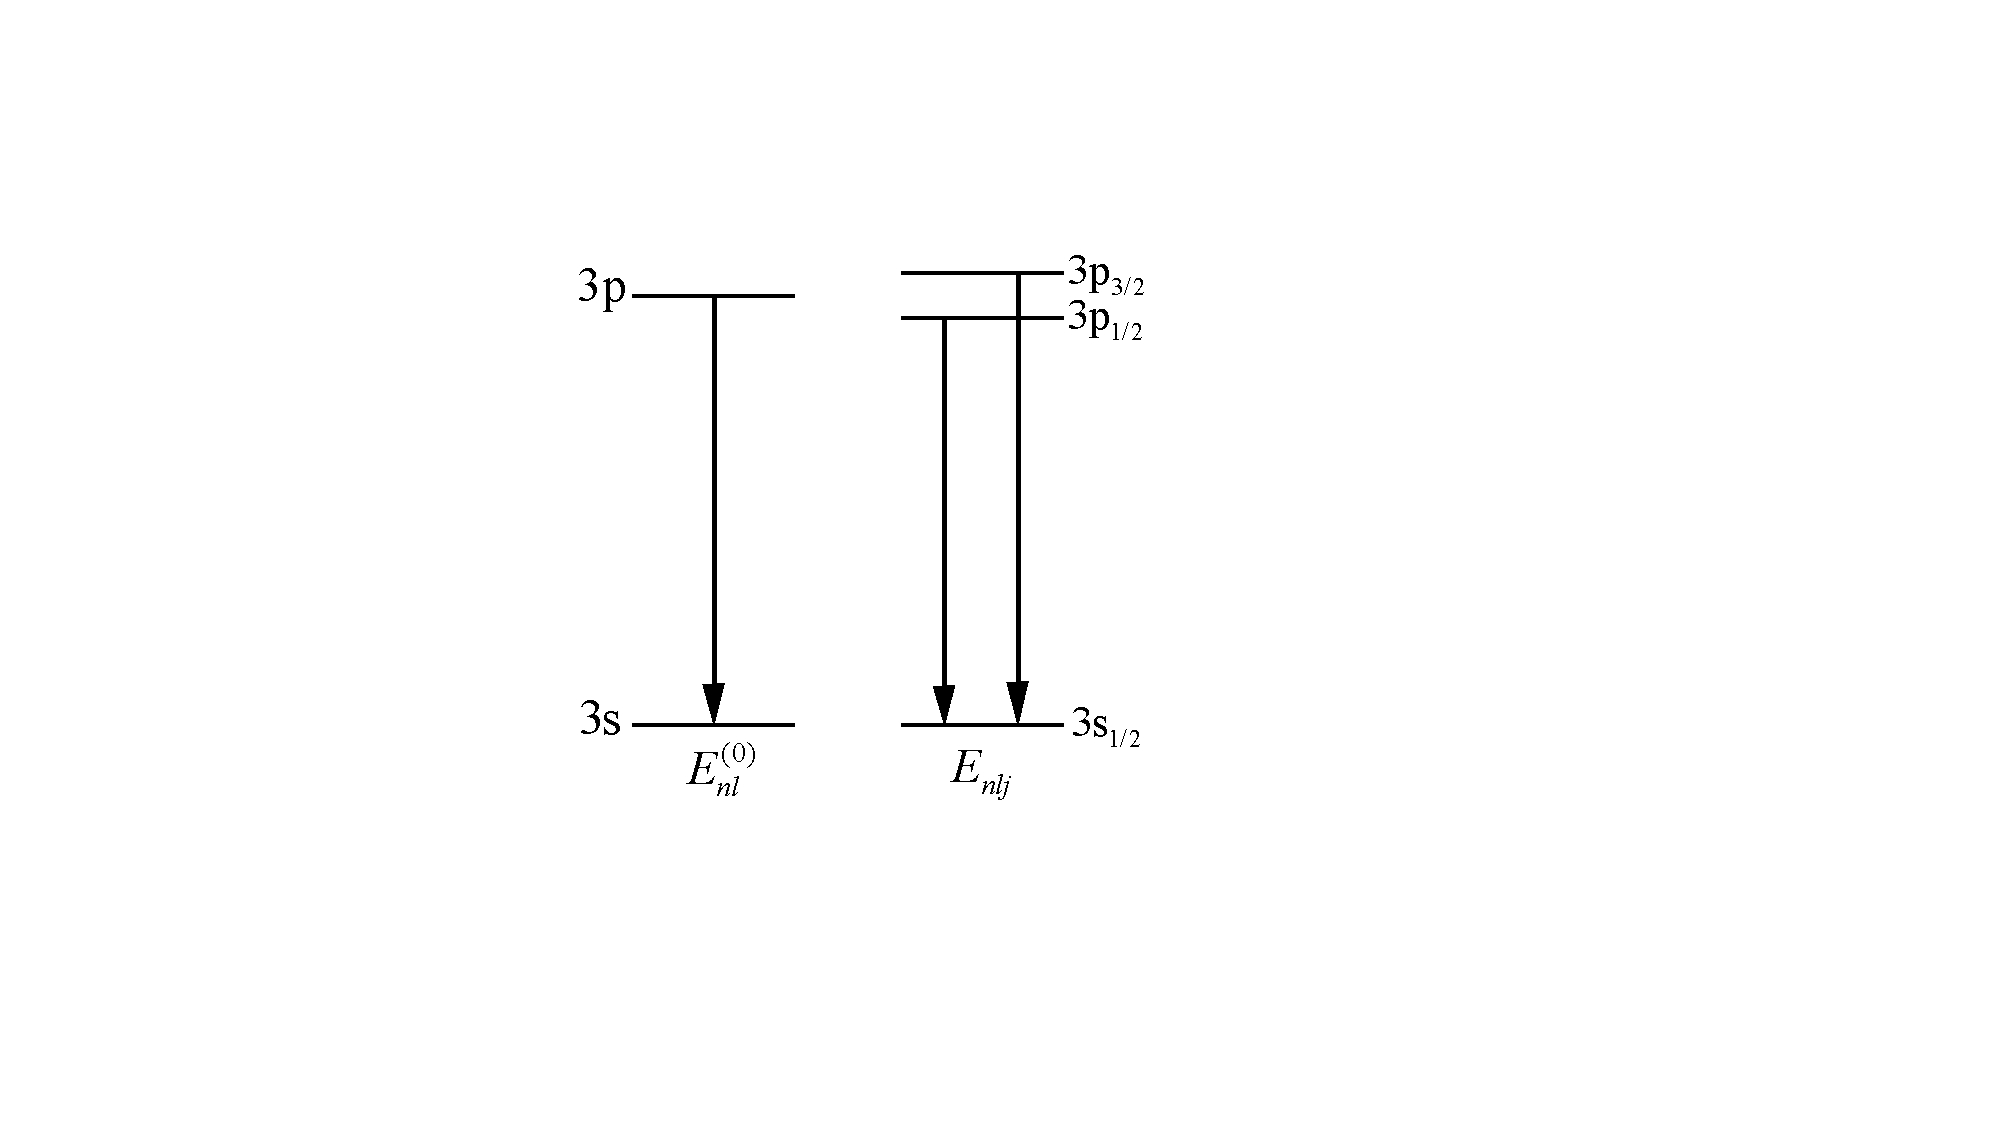
\includegraphics[width=3cm,clip]{QM file/figure/7-1}
	\caption{}\label{fig.7-1}
\end{wrapfigure}
由于自旋轨道耦合作用,能级$E_{nl}^{(0)}$分裂成两个能级,$j=l+\frac{1}{2}$者较高$(E_{nlj}^{(1)}>0)$,$j=l-\frac{1}{2}$者较低$(E_{nlj}^{(1)}<0)$,裂距
\eqllong
\begin{empheq}{align}\label{eq73.15}
	\Delta E&=E_{nl,l+\frac{1}{2}}^{(1)}-E_{nl,l-\frac{1}{2}}^{(1)}	\nonumber\\
	&=\bigg(l+\frac{1}{2}\bigg)\hbar^{2}\langle\xi(r)\rangle 
\end{empheq}\eqnormal
但s态例外,s态$\boldsymbol{S}\cdot\boldsymbol{L}\text{(本征值)}=0$,没有自旋轨道耦合能,能级不分裂.

能级分裂的示意图见图\ref{fig.7-1},图中画出了3p$(n=3,l=1)$能级的分裂情况与此相应,跃迁3p$\rightarrow$3s造成的光谱线也分裂成两条,这就是光谱线的精细结构.










% 粒子在电磁场中的运动
\starthis\section[粒子在电磁场中的运动]{粒子在电磁场中的运动} \label{sec:07.04} % 
% \makebox[5em][s]{} % 短题目拉间距

{\heiti 1. 自旋为零的粒子}

以$m$和$q$表示粒子的质量和电荷,而自旋为零.当粒子在电磁场中运动时,按照经典电动力学,哈密顿量为
\begin{empheq}{equation}\label{eq74.1}
	H=\frac{1}{2m}\bigg(\boldsymbol{p}-\frac{q}{c}\boldsymbol{A}\bigg)^{2}+q\phi
\end{empheq}
其中$\boldsymbol{p}$是粒子的正则动量,$\phi$和$\boldsymbol{A}$是电磁场的标势和矢势,它们与电场$\mathscr{E}$和磁场$B$的关系是
\begin{empheq}{equation}\label{eq74.2}
	\mathscr{E}=-\nabla\phi-\frac{1}{c}\frac{\partial\boldsymbol{A}}{\partial t},\quad \boldsymbol{B}=\nabla\times\boldsymbol{A}
\end{empheq}
由\eqref{eq74.1}式并利用正则方程
\begin{empheq}{equation}\label{eq74.3}
	\dot{x}_{i}=\frac{\partial H}{\partial p_{i}}\quad \dot{p}_{i}=-\frac{\partial H}{\partial x_{i}}
\end{empheq}
可以证明粒子的机械动量是
\begin{empheq}{equation}\label{eq74.4}
	m\boldsymbol{v}=m\frac{d}{dt}\boldsymbol{r}=\boldsymbol{p}-\frac{q}{c}\boldsymbol{A}
\end{empheq}
并可导出粒子的经典运动方程
\begin{empheq}{equation}\label{eq74.5}
	m\frac{d\boldsymbol{v}}{dt}=q\mathscr{E}+\frac{q}{c}\boldsymbol{v}\times\boldsymbol{B}
\end{empheq}
第一项为电场的作用力,第二项为磁场的作用力,即洛伦兹力.

推广到量子力学,只需将$\boldsymbol{p}$换成算符,即令
\eqshort
\begin{empheq}{equation}\label{eq74.6}
	\hat{\boldsymbol{p}}=-i\hbar\nabla
\end{empheq}\eqnormal
就得到哈密顿算符
\begin{empheq}{equation}\label{eq74.7}
	\hat{H}=\frac{1}{2m}\bigg(\hat{\boldsymbol{p}}-\frac{q}{c}\boldsymbol{A}\bigg)^{2}+q\phi
\end{empheq}
如定义速度算符
\begin{empheq}{equation}\label{eq74.8}
	\hat{\boldsymbol{v}}=\frac{d\hat{\boldsymbol{r}}}{dt}=\frac{1}{i\hbar}[\boldsymbol{r},\hat{H}]
\end{empheq}
容易求出
\begin{empheq}{equation}\label{eq74.9}
	\hat{\boldsymbol{v}}=\frac{1}{m}\bigg(\hat{\boldsymbol{p}}-\frac{q}{c}\boldsymbol{A}\bigg)
\end{empheq}
上式正是经典关系\eqref{eq74.4}式的量子力学推广.\eqref{eq74.7}式也可以写成
\begin{empheq}{equation}\label{eq74.10}
	\hat{H}=\frac{1}{2}m\hat{\boldsymbol{v}}^{2}+q\phi
\end{empheq}
\eqref{eq74.7}式中
\begin{empheq}{equation*}
	\bigg(\hat{\boldsymbol{p}}-\frac{q}{c}\boldsymbol{A}\bigg)^{2}=\hat{\boldsymbol{p}}^{2}+\frac{q^{2}}{c^{2}}\boldsymbol{A}^{2}-\frac{q}{c}(\hat{\boldsymbol{p}}\cdot\boldsymbol{A}+\boldsymbol{A}\cdot\hat{\boldsymbol{p}})
\end{empheq}
其中
\begin{empheq}{equation*}
	\hat{\boldsymbol{p}}\cdot\boldsymbol{A}+\boldsymbol{A}\cdot\hat{\boldsymbol{p}}=-i\hbar(\nabla\cdot\boldsymbol{A})+2\boldsymbol{A}\cdot\hat{\boldsymbol{p}}
\end{empheq}
即一般$\hat{\boldsymbol{p}}\cdot\boldsymbol{A}\neq\boldsymbol{A}\cdot\hat{\boldsymbol{p}}$.但如规定矢势$\boldsymbol{A}$满足横波条件$\nabla\cdot\boldsymbol{A}=0$,则$\boldsymbol{p}\cdot\boldsymbol{A}=\boldsymbol{A}\cdot\hat{\boldsymbol{p}}=-i\hbar\boldsymbol{A}\cdot\nabla$,这时$\hat{H}$可以化成
\eqlong
\begin{empheq}{align*}\label{eq74.7'}
	\hat{H}&=\frac{\hat{\boldsymbol{p}}^{2}}{2m}-\frac{q}{mc}\boldsymbol{A}\cdot\hat{\boldsymbol{p}}+\frac{q^{2}}{2mc^{2}}\boldsymbol{A}^{2}+q\phi	\\
	&=-\frac{\hbar^{2}}{2m}\nabla^{2}+i\frac{\hbar q}{mc}\boldsymbol{A}\cdot\nabla+\frac{q^{2}}{2mc^{2}}\boldsymbol{A}^{2}+q\phi	\tag{$7.4.7^{\prime}$}\eqnormal
\end{empheq}

薛定谔方程仍为
\eqshort
\begin{empheq}{equation}\label{eq74.11}
	i\hbar\frac{\partial}{\partial t}\varPsi=\hat{H}\varPsi 
\end{empheq}\eqnormal
写开来,就是
\eqllong
\begin{empheq}{equation*}\label{eq74.11'}
	i\hbar\frac{\partial\varPsi}{\partial t}=-\frac{\hbar^{2}}{2m}\nabla^{2}\varPsi+i\frac{\hbar q}{mc}\boldsymbol{A}\cdot\nabla\varPsi+\frac{q^{2}}{2mc^{2}}\boldsymbol{A}^{2}\varPsi+q\phi\varPsi	\tag{$7.4.11^{\prime}$}
\end{empheq}\eqnormal
下面导出连续性方程.上式的共轭方程为
\eqindent{2}
\begin{empheq}{equation*}\label{eq74.11''}
	i\hbar\frac{\partial\varPsi^{*}}{\partial t}=-\frac{\hbar^{2}}{2m}\nabla^{2}\varPsi^{*}+i\frac{\hbar q}{mc}\boldsymbol{A}\cdot\nabla\varPsi^{*}+\frac{q^{2}}{2mc^{2}}\boldsymbol{A}^{2}\varPsi^{*}+q\phi\varPsi^{*}	\tag{$7.4.11^{\prime\prime}$}
\end{empheq}\eqnormal
用$\varPsi^{*}$左乘\eqref{eq74.11'}式,$\varPsi$左乘\eqref{eq74.11''}式,相减,即得
\eqllong
\begin{empheq}{align*}
	i\hbar\frac{\partial}{\partial}(\varPsi^{*}\varPsi) =&-\frac{\hbar^{2}}{2m}(\varPsi^{*}\nabla^{2}\varPsi-\varPsi\nabla^{2}\varPsi^{*})	\\
	&+i\frac{\hbar q}{mc}\boldsymbol{A}\cdot(\varPsi^{*}\nabla+\varPsi\nabla\varPsi^{*})	\\
	=&-\frac{\hbar^{2}}{2m}\nabla\cdot(\varPsi^{*}\nabla\varPsi-\varPsi\nabla\varPsi^{*})+i\frac{\hbar q}{mc}\nabla\cdot(\boldsymbol{A}\varPsi^{*}\varPsi)
\end{empheq}\eqnormal
上式实质上就是连续性方程
\begin{empheq}{equation}\label{eq74.12}
	\frac{\partial\rho}{\partial t}+\nabla\cdot\boldsymbol{j}=0
\end{empheq}
其$\rho=\varPsi^{*}\varPsi$为概率密度,$\boldsymbol{j}$为概率流密度,
\begin{empheq}{equation}\label{eq74.13}
	\boldsymbol{j}=\frac{i\hbar}{2m}(\varPsi^{*}\nabla\varPsi-\varPsi\nabla\varPsi^{*})-\frac{q}{mc}\boldsymbol{A}\varPsi^{*}\varPsi
\end{empheq}
亦即
\begin{empheq}{align*}\label{eq74.13'}
	\boldsymbol{j}&=\frac{1}{2m}\varPsi^{*}\bigg(\hat{\boldsymbol{p}}-\frac{q}{c}\boldsymbol{A}\bigg)\varPsi+c.c.	\\
	&=\frac{1}{2}\varPsi^{*}\hat{\boldsymbol{v}}\varPsi+c.c.=\Re(\varPsi^{*}\hat{\boldsymbol{v}}\varPsi)
	\tag{$7.4.13^{\prime}$}
\end{empheq}
电荷密度及电流密度为
\begin{empheq}{align}
	&\rho_{n}=q\rho=q\varPsi^{*}\varPsi		\label{eq74.14}\\
	\boldsymbol{j}_{e}=q\boldsymbol{j}=\frac{q}{2}&\varPsi^{*}\hat{\boldsymbol{v}}\varPsi+c.c.=\Re(q\varPsi^{*}\hat{\boldsymbol{v}}\varPsi)		\label{eq74.15}
\end{empheq}
而在经典物理中$\boldsymbol{j}_{e}=\boldsymbol{v}\rho_{e}$.

{\heiti 2. 电子}

电子(电荷$q=-e$)具有自旋磁矩
\begin{empheq}{equation}\label{eq74.16}
	\boldsymbol{\mu}_{s}=-\frac{e}{m_{e}c}\boldsymbol{S}=-\frac{e\hbar}{2m_{n}c}\boldsymbol{\sigma}
\end{empheq}
当电子在电磁场中运动时,磁场$\boldsymbol{B}$对磁矩$\boldsymbol{\mu}_{s}$的作用势是
\begin{empheq}{equation}\label{eq74.17}
	-\boldsymbol{B}\cdot\boldsymbol{\mu}_{s}=\frac{e\hbar}{2m_{n}c}\boldsymbol{B}\cdot\boldsymbol{\sigma}
\end{empheq}
将\eqref{eq74.17}式和\eqref{eq74.7}式合起来,就是在电磁场中的电子哈密顿算符:
\begin{empheq}{equation}\label{eq74.18}
	\hat{H}=\frac{1}{2m_{e}}\bigg(\hat{\boldsymbol{p}}+\frac{e}{c}\boldsymbol{A}\bigg)^{2}-e\phi+\frac{e\hbar}{2m_{n}c}\boldsymbol{B}\cdot\boldsymbol{\sigma}
\end{empheq}
薛定谔方程形式上仍取\eqref{eq74.11}式的形式,但是波函数$\varPsi$($xyzS_{z}$表象)应表示成二分量的列矢量:
\begin{empheq}{equation}\label{eq74.19}
	\varPsi=\begin{bmatrix}
		\varPsi_{1}(xyz,t)	\\	\varPsi_{2}(xyz,t)
	\end{bmatrix}
\end{empheq}
薛定谔方程表现为
\begin{empheq}{equation}\label{eq74.20}
	i\hbar\frac{\partial}{\partial t}\begin{bmatrix}
		\varPsi_{1}	\\	\varPsi_{2}
	\end{bmatrix}=\hat{H}\begin{bmatrix}
		\varPsi_{1}	\\	\varPsi_{2}
\end{bmatrix}
\end{empheq}
习惯上称为泡利方程.仿照\eqref{eq74.11}式以下的步骤,不难导出连续性方程,从而得到概率密度$\rho$,概率流密度$\boldsymbol{j}$,电荷密度$\rho_{e}$,电流密度$\boldsymbol{j}_{e}$的公式.结果如下:
\begin{empheq}{equation}\label{eq74.21}
	\rho=\varPsi^{*}\varPsi=\varPsi_{1}^{*}\varPsi_{1}+\varPsi_{2}^{*}\varPsi_{2}	
\end{empheq}
\begin{empheq}{align}\label{eq74.22}
	\boldsymbol{j}&=\frac{1}{2m_{e}}\varPsi^{+}\bigg(\hat{\boldsymbol{p}}+\frac{e}{c}\boldsymbol{A}\bigg)\varPsi+c.c.=\Re(\varPsi^{*}\hat{\boldsymbol{v}}\varPsi)	\nonumber\\
	&=\Re(\varPsi_{1}^{*}\hat{\boldsymbol{v}}\varPsi_{1}+\varPsi_{2}^{*}\hat{\boldsymbol{v}}\varPsi_{2})
\end{empheq}
\begin{empheq}{equation}\label{eq74.23}
	\rho_{e}=-e\rho,\quad \boldsymbol{j}_{e}=-e\boldsymbol{j}
\end{empheq}
注意这些最均与自旋算符无关,因为它们反映电子的空间分布与流动情况,而自旋自由度与此无关.

{\heiti 3. 均匀磁场中的原子}

以单价原子为例,说明一下物质的磁性起源.原子的最外层电子(价电子)容易受外场的影响,原子的电磁性质在很大程度上取决于价电子.将原子置于均匀磁场中,以$\boldsymbol{B}$方向为$z$轴方向,则磁场为
\begin{empheq}{equation*}
	B_{x}=B_{y}=0,\quad B_{z}=B
\end{empheq}
矢势$\boldsymbol{A}$可以取为
\begin{empheq}{equation}\label{eq74.24}
	A_{x}=-\frac{B}{2}y,\quad A_{y}=\frac{B}{2}x,\quad A_{z}=0
\end{empheq}
并已满足横波条件$\nabla\cdot\boldsymbol{A}=0$,因此
\begin{empheq}{equation*}
	\hat{\boldsymbol{p}}\cdot\boldsymbol{A}=\boldsymbol{A}\cdot\hat{\boldsymbol{p}}=\frac{B}{2}(x\hat{p}_{y}-y\hat{p}_{x})=\frac{B}{2}\hat{L}_{z}
\end{empheq}
代入\eqref{eq74.18}式,[利用\eqref{eq74.7}式的展开\eqref{eq74.7'}式]得到
\eqllong
\begin{empheq}{equation}\label{eq74.25}
	\hat{H}=\frac{1}{2m_{e}}\hat{\boldsymbol{p}}^{2}+V(r)+\frac{eB}{2m_{e}c}(\hat{L}_{z}+2\hat{S}_{z})+\frac{e^{2}B^{2}}{8m_{e}c^{2}}(x^{2}+y^{2})
\end{empheq}
其中$V(r)$表示原子核与内层电子对于价电子的库仑作用势的总和,即\eqref{eq74.18}式中$(-e\phi)$项的等效表示.\eqref{eq74.25}式中前两项是原子中价电子本来的能量算符,后两项是磁作用能.由此可以求得原子的磁矩
\begin{empheq}{equation}\label{eq74.26}
	\hat{\mu_{z}}=-\frac{\partial\hat{H}}{\partial B}=-\frac{e}{2m_{e}c}(\hat{L}_{z}+2\hat{S}_{z})-\frac{e^{2}B}{4m_{e}c^{2}}(x^{2}+y^{2})
\end{empheq}\eqnormal
其中第一项是原子的固有磁矩(轨道磁矩及自旋磁矩).第二项与磁场$B$成正比,为诱导磁矩,它总是负的,属于逆磁性效应.按量级而言,第二项远小于第一项,因此只有固有磁矩为零的原子(如惰气原子及许多二价原子)逆磁性才能表现出来.

\eqref{eq74.26}式中,第一项量级与玻尔磁子相同,
\begin{empheq}{equation*}
	\mu_{B}=\frac{e\hbar}{2m_{e}c}=\num{5.8}\times 10^{-9}\si{eV/Gs}
\end{empheq}
第二项的量级约为
\eqlong
\begin{empheq}{align*}
	\frac{e^{2}B}{4m_{e}c^{2}}(x^{2}+y^{2})&\sim B\frac{e^{2}a_{0}^{2}}{4m_{e}c^{2}}\bigg(\frac{\hbar^{2}}{m_{e}e^{2}}\bigg)^{2}	\\
	&\sim\frac{B\mu_{B}^{2}}{m_{e}c^{2}}\bigg(\frac{\hbar c}{e^{2}}\bigg)^{2}\sim B\times10^{-18}\si{eV/Gs^{2}}
\end{empheq}
当$\boldsymbol{B}\sim10^{5}\si{Gs}$,第二项量级约为$10^{-13}\si{eV/Gs}$,仅为$\mu_{B}$的$10^{-4}$倍.

\example 求速度算符$\hat{\boldsymbol{v}}$各分量间的对易式.

\solution 以$[\hat{v}_{x},\hat{v}_{y}]$为例,按照\eqref{eq74.9}式,
\begin{empheq}{align}\label{eq74.27}
	[\hat{v}_{x},\hat{v}_{y}]&=\frac{1}{m^{2}}\bigg[\hat{p}_{x}-\frac{q}{c}A_{x},\quad \hat{p}_{y}-\frac{q}{c}A_{y}\bigg]	\nonumber\\
	&=-\frac{q}{m^{2}c}([\hat{p}_{x},A_{y}]+[A_{x},\hat{p}_{y}])	\nonumber\\	% $\hat{p}_{y}$?
	&=-\frac{q}{m^{2}c}(-i\hbar)\bigg(\frac{\partial A_{y}}{\partial x}-\frac{\partial A_{x}}{\partial y}\bigg)=i\frac{\hbar q}{m^{2}c}B_{z}
\end{empheq}\eqnormal
类似地有
\begin{empheq}{equation*}
	[\hat{v}_{y},\hat{v}_{z}]=i\frac{\hbar q}{m^{2}c}B_{x},\quad [\hat{v}_{z},\hat{v}_{x}]=i\frac{\hbar q}{m^{2}c}B_{y}
\end{empheq}
$\boldsymbol{B}=\nabla\times\boldsymbol{A}$写成矢量形式,就是
\begin{empheq}{equation*}\label{eq74.27'}
	\hat{\boldsymbol{v}}\times\hat{\boldsymbol{v}}=i\frac{\hbar q}{m^{2}c}\boldsymbol{B}
	\tag{$7.4.27^{\prime}$}
\end{empheq}
$\boldsymbol{B}=\nabla\times\boldsymbol{A}$
是磁场,进一步还可算出
\begin{empheq}{equation}\label{eq74.28}
	[\hat{\boldsymbol{v}},\hat{\boldsymbol{v}}^{2}]=i\frac{\hbar q}{m^{2}c}(\hat{\boldsymbol{v}}\times\boldsymbol{B}-\boldsymbol{B}\times\hat{\boldsymbol{v}})
\end{empheq}

% 塞曼效应
\section[塞曼效应]{塞曼效应} \label{sec:07.05} % 
% \makebox[5em][s]{} % 短题目拉间距

早在19世纪末就已经发现磁场能够影响原子光谱.1896年塞曼发现,如将光源放在磁场中,则每一条光谱线均分裂成一组相邻的线.这种现象称为塞曼效应.

显然, 谱线分裂的根源是能级分裂.以单价原子为例,其光谱产生于价电子的能级跃迁未加磁场前,价电子的能量算符可以写成(参看$\S$\ref{sec:07.03})
\begin{empheq}{equation}\label{eq75.1}
	H_{0}=\frac{\boldsymbol{p}^{2}}{2m_{e}}+V(r)+\xi(r)\boldsymbol{S}\cdot\boldsymbol{L}
\end{empheq}
最后一项是自旋轨道耦合能加上磁场后,价电子又获得一项磁作用势,以磁场方向为$z$轴,磁作用势为
\begin{empheq}{equation}\label{eq75.2}
	H^{\prime}=-\boldsymbol{B}\cdot(\boldsymbol{\mu_{L}}+\boldsymbol{\mu_{S}})=\frac{eB}{2m_{e}c}(L_{z}+2S_{z})
\end{empheq}
[参看\eqref{eq74.25}式,略去很小的逆磁性项($B^{2}$项).]价电子的总能量算符变成
\eqshort
\begin{empheq}{equation}\label{eq75.3}
	H=H_{0}+H^{\prime}
\end{empheq}\eqnormal
由$H^{\prime}$造成的能级分裂,视磁场的强弱而有所不同.

{\heiti 1. 强磁场,简单塞曼效应}

如磁场很强(至少要几十万高斯),以致\eqref{eq75.1}式中自旋轨道耦合能可以忽略不计,这时价电子的能量算符为
\begin{empheq}{equation}\label{eq75.4}
	H=\frac{\boldsymbol{p}^{2}}{2m_{e}}+V(r)+\frac{eB}{2m_{e}c}(L_{z}+2S_{z})
\end{empheq}
其中第三项为磁作用势.这时$H,H_{0},\boldsymbol{L}^{2},L_{z},S_{z}$是互相对易的守恒量.如以$E_{nl}^{(0)}$表示$H_{0}=(\hat{T}+V)$的本征值(未加磁场时的价电子能级),$\varPsi_{nlm}=R_{nl}(r)Y_{lm}(\theta\varphi)$表示$(H_{0},\boldsymbol{L}^{2},L_{z})$共同本征函数,则$(H,\boldsymbol{L}^{2},L_{z},S_{z})$的共同本征函数显然是
\begin{empheq}{equation}\label{eq75.5}
	\varPsi_{nlmm_{s}}=\varPsi_{nlm}\chi_{1/2},\quad \varPsi_{nlm}\chi_{-1/2}
\end{empheq}
前者$S_{z}=\frac{\hbar}{2}\bigg(m_{s}=\frac{1}{2}\bigg)$,后者$S_{z}=-\frac{\hbar}{2}\bigg(m_{s}=-\frac{1}{2}\bigg)$.能级可以记成$E=E_{nlmm_{s}}$,显然
\begin{empheq}{align}\label{eq75.6}
	E_{nlmm_{s}}&=E_{nl}^{(0)}+B\mu_{B}(m+2m_{s})	\nonumber\\
	&=E_{nl}^{(0)}+\begin{dcases}
		(m+1)B\mu_{B},\quad m_{s}=\frac{1}{2}	\\
		(m-1)B\mu_{B},\quad m_{s}=-\frac{1}{2}
	\end{dcases}
\end{empheq}
$\bigg(\mu_{B}$为玻尔磁子$\bigg)$上式表明,能级$E_{nl}^{(0)}$在磁场中分裂成一组等距离的能级,能级间距为$B\mu_{B}$.由能级跃迁产生的光谱线也有分裂现象,由于跃迁选择定则:
\begin{empheq}{equation}\label{eq75.7}
	\Delta l=\pm1,\quad \Delta m=0,\pm1,\quad \Delta m_{s}=0
\end{empheq}
的限制,每条谱线在磁场中分裂成三条等距离的谱线.能级和谱线的分裂如图\ref{fig.7-2}所示.

\begin{figure}[!h]
	\centering
	\small
	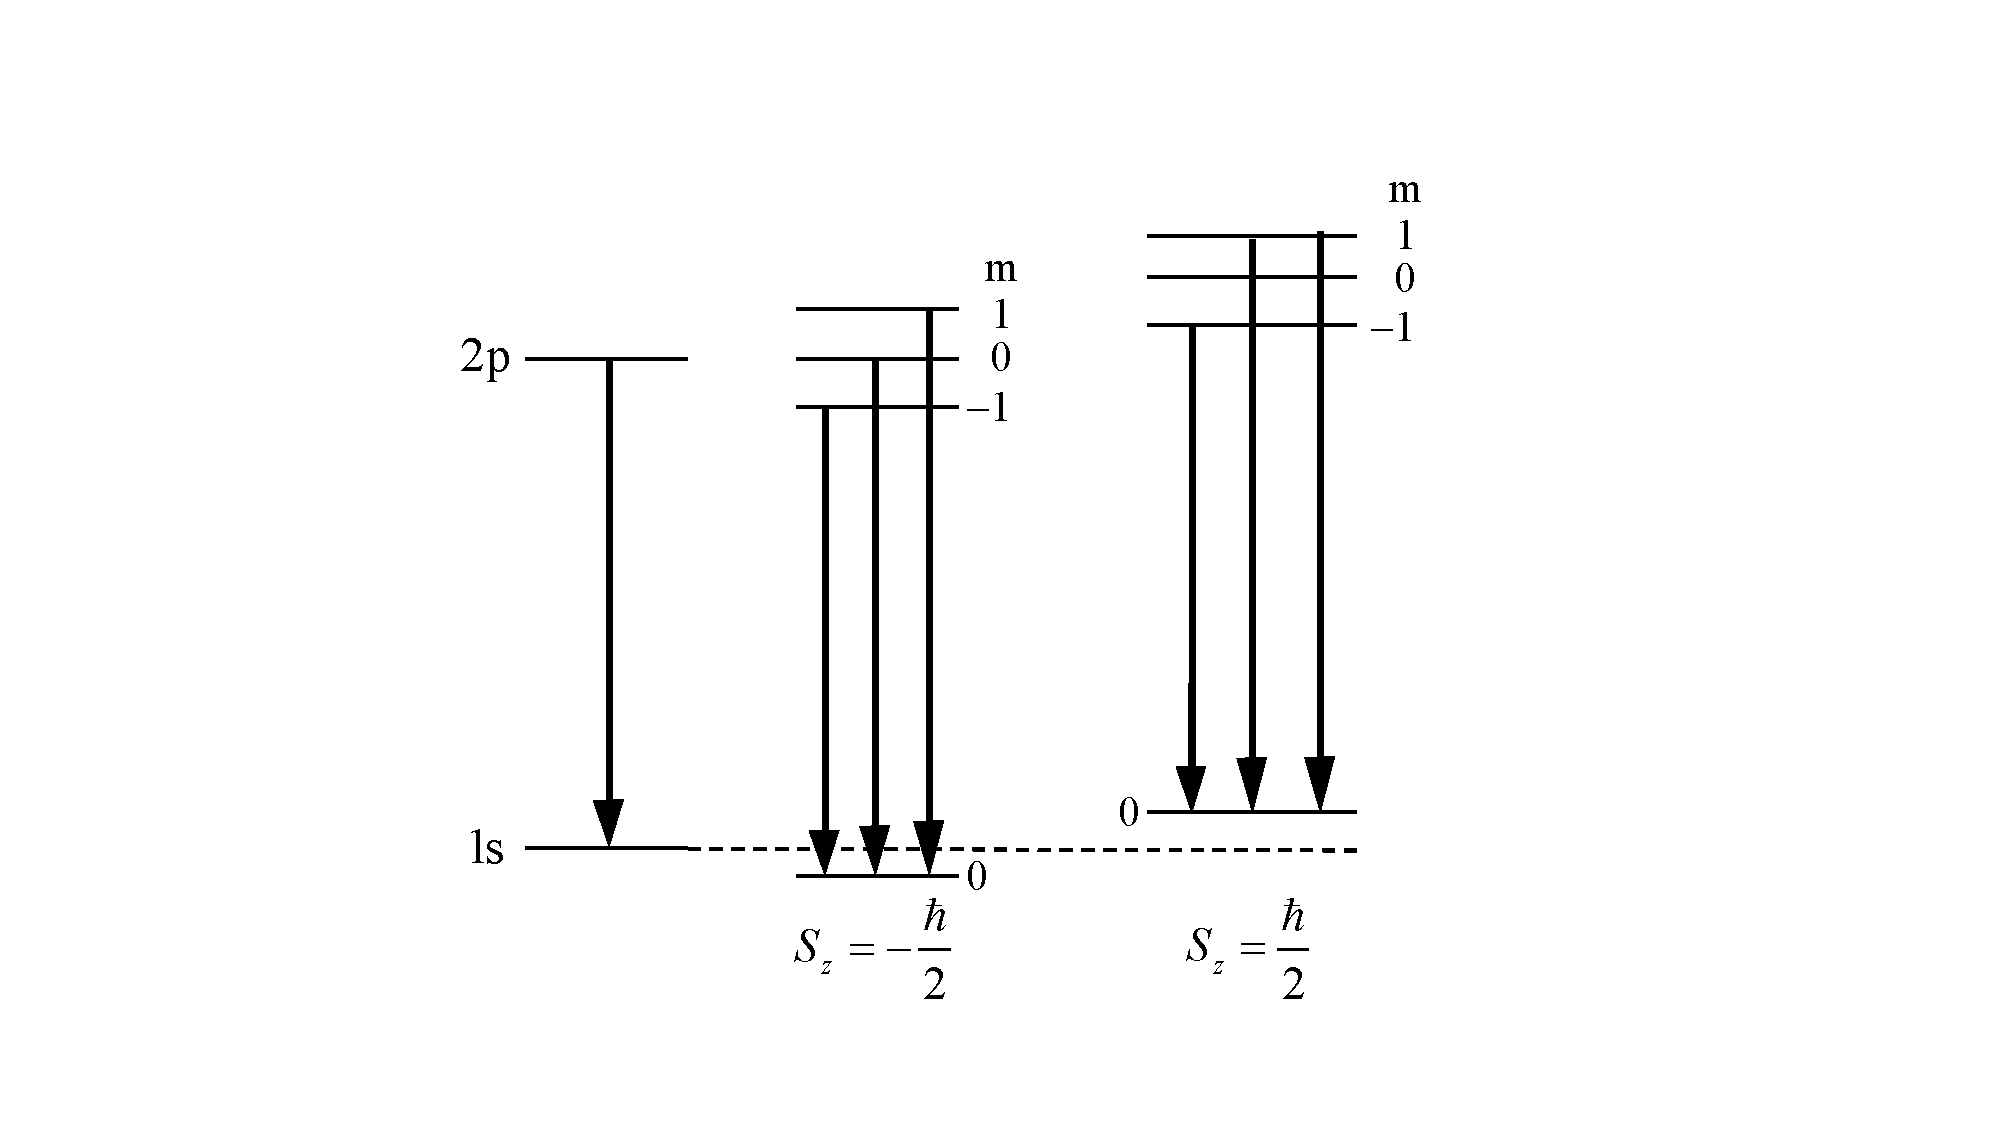
\includegraphics[width=5cm,clip]{QM file/figure/7-2}
	\caption{}\label{fig.7-2}
\end{figure}

图\ref{fig.7-2}画出了能级$E_{21}^{(0)}$,$E_{10}^{(0)}$在强磁场中的分裂示意图,以及符合选择定则的能级跃迁.由于跃迁前后自旋量子数$m_{s}$不变,图中两组跃迁产生的光谱相同,均包含三条谱线.相邻谱线的频率差为
\begin{empheq}{equation}\label{eq75.8}
	\Delta\omega=\frac{B\mu_{B}}{\hbar}=\frac{eB}{2m_{e}c}
\end{empheq}
刚好等于经典拉摩频率.这种现象,称为简单塞曼效应\footnote{
单价原子光谱在强磁场中的分裂现象,严格说应称为帕邢-巴克(Paschen-Back)效应.纯粹的简单塞曼效应只产生于价电子为偶数,总自旋角动量$S=0$的情况下,这时自旋轨道耦合能为0.磁作用势
\begin{empheq}{equation*}
	H^{\prime}=-\boldsymbol{B}\cdot\mu_{L}=\frac{eB}{2m_{e}c}L_{z}
\end{empheq}
($\boldsymbol{L}$为总轨道角动量)能级变化为$H^{\prime}=mB\mu_{B}(L_{z}=m\hbar)$,能级$E_{nl}^{(0)}$分裂成$(2L+1)$条等距离能级,间距$\Delta E=B\mu_{B}$.由于跃迁选择定则\eqref{eq75.7}式的制约,光谱线仍分裂为三条等距离的谱线,$\Delta\omega$仍由\eqref{eq75.8}式表示.这种效应只需要弱磁场就能产生,而且可以给以经典电动力学解释,所以曾称为正常塞曼效应.其实下面要讲的复杂塞曼效应才是塞曼效应的一般表现形式,由于它无法用经典物理理论来解释,曾被称为“反常”的.}由于$\Delta\omega$与$\hbar$无关,历史上曾根据经典电动力学的拉摩进动模型给出了很好的定量解释.

{\heiti 2. 弱磁场,复杂塞曼效应}

在弱磁场中,单价原子受到的磁作用势小于自旋轨道耦合能,应将\eqref{eq75.3}式中$H^{\prime}$作为微扰.取$(H_{0},\boldsymbol{L}^{2},\boldsymbol{J}^{2},J_{z})$共同本征函数作为零级近似波函数,记为
\begin{empheq}{equation}\label{eq75.9}
	\Psi_{nljm_{j}}^{(0)}=R_{nl}(r)\varPsi_{ljm_{j}}(\theta,\varphi,S_{z})
\end{empheq}
其中$\varPsi_{ljm_{j}}$表示$(\boldsymbol{L}^{2},\boldsymbol{J}^{2},J_{z})$共同本征函数(见$\S$\ref{sec:07.02}).$H_{0}$由\eqref{eq75.1}式表示,其中包含了自旋轨道耦合能.$H_{0}$的本征值即未加磁场时的价电子能级,和量子数$nlj$有关,但和$m_{j}$无关,(见$\S$\ref{sec:07.03})可以记为$E_{nlj}^{(0)}$,能级简并度$(2j+1)$.给定$n,l$后,$j=l\pm\frac{1}{2}$对应于两个能级,就是能级的精细结构(见$\S$\ref{sec:07.03}).

按照简并态微扰论计算磁作用势$H^{\prime}$造成的能级变化(一级修正).由于$H^{\prime}$与$J_{z}$对易,因此$H^{\prime}$的非对角矩阵元全部等于0,能级的一级修正等于$H^{\prime}$对\eqref{eq75.9}式的平均值,即
\eqlong
\begin{empheq}{align}\label{eq75.10}
	E_{nljm_{j}}^{(1)} &=\int\Psi_{nljm_{j}}^{(0)+}\hat{H}\Psi_{nljm_{j}}^{(0)}d\tau	\nonumber\\
	&=\frac{eB}{2m_{e}c}(\overline{J_{z}}+\overline{S_{z}})=\frac{eB}{2m_{e}c}\bigg(m_{j}\hbar+\frac{\hbar}{2}\overline{\sigma_{z}}\bigg)
\end{empheq}\eqnormal
其中$\overline{\sigma_{z}}$已在\eqref{eq72.23}式、\eqref{eq72.24}式算出,为
\begin{empheq}{align}\label{eq75.11}
	\overline{\sigma_{z}}=
	\begin{dcases}
		\quad\frac{m_{j}}{j},\qquad j=l+\frac{1}{2}	\\
		-\frac{m_{j}}{j+1},\quad j=l-\frac{1}{2}
	\end{dcases}
\end{empheq}
代入\eqref{eq75.10}式, 即得
\begin{empheq}{equation}\label{eq75.12}
	E_{nljm_{j}}^{(1)}=B\mu_{B}m_{j}g
\end{empheq}
其中$g$为朗德$g$因子,即
\eqlong
\begin{empheq}{align}\label{eq75.13}
	g &=1+\frac{\langle\sigma_{z}\rangle}{2m_{j}}=1+\frac{\langle S_{z}\rangle}{\langle J_{z}\rangle}	\\
	&=\begin{dcases}
		1+\frac{1}{2j},\qquad\quad	j=l+\frac{1}{2}	\\
		1-\frac{1}{2j+2},\quad j=l-\frac{1}{2}	
	\end{dcases}	\nonumber \tag{$7.5.13^{\prime}$}
\end{empheq}\eqnormal
这样, 由\eqref{eq75.12}式、\eqref{eq75.13}式可知,能级$E_{nlj}^{(0)}$在弱磁场中分裂成$(2j+1)$个等距离能级,相应于$m_{j}$的$(2j+1)$种取值
\begin{empheq}{equation}\label{eq75.14}
	m_{j}=j,j-1,\cdots,(-j)
\end{empheq}
能级间距为$B\mu_{B}g$.(在简单塞曼效应中,能级分裂间距为$B\mu_{B}$)因此,对光谱进行实验分析浏定,可以推断出能级的$g$和$j$值(由此也就知道$l$值),这样就获得了有关原子结构的重要信息.

能级跃迁的选择定则是
\begin{empheq}{equation}\label{eq75.15}
	\Delta l=\pm1,\quad \Delta j=0,\pm1,\quad \Delta m_{j}=0,\pm1
\end{empheq}
图\ref{fig.7-3}画出了钠(\ce{Na})的$D_{1}$和$D_{2}$线的分裂示意图.能级和谱线的分裂均比简单塞曼效应复杂,故称复杂塞曼效应.发现这现象的当时,无法对此作出理论解释,故又称反常塞曼效应.直到1925年乌仑贝克(Uhlenbeck)与古兹米特(Goudsmit)提出电子自旋假设,这个“反常”现象才得到解释.

\begin{figure}[!h]
	\centering
	\small
	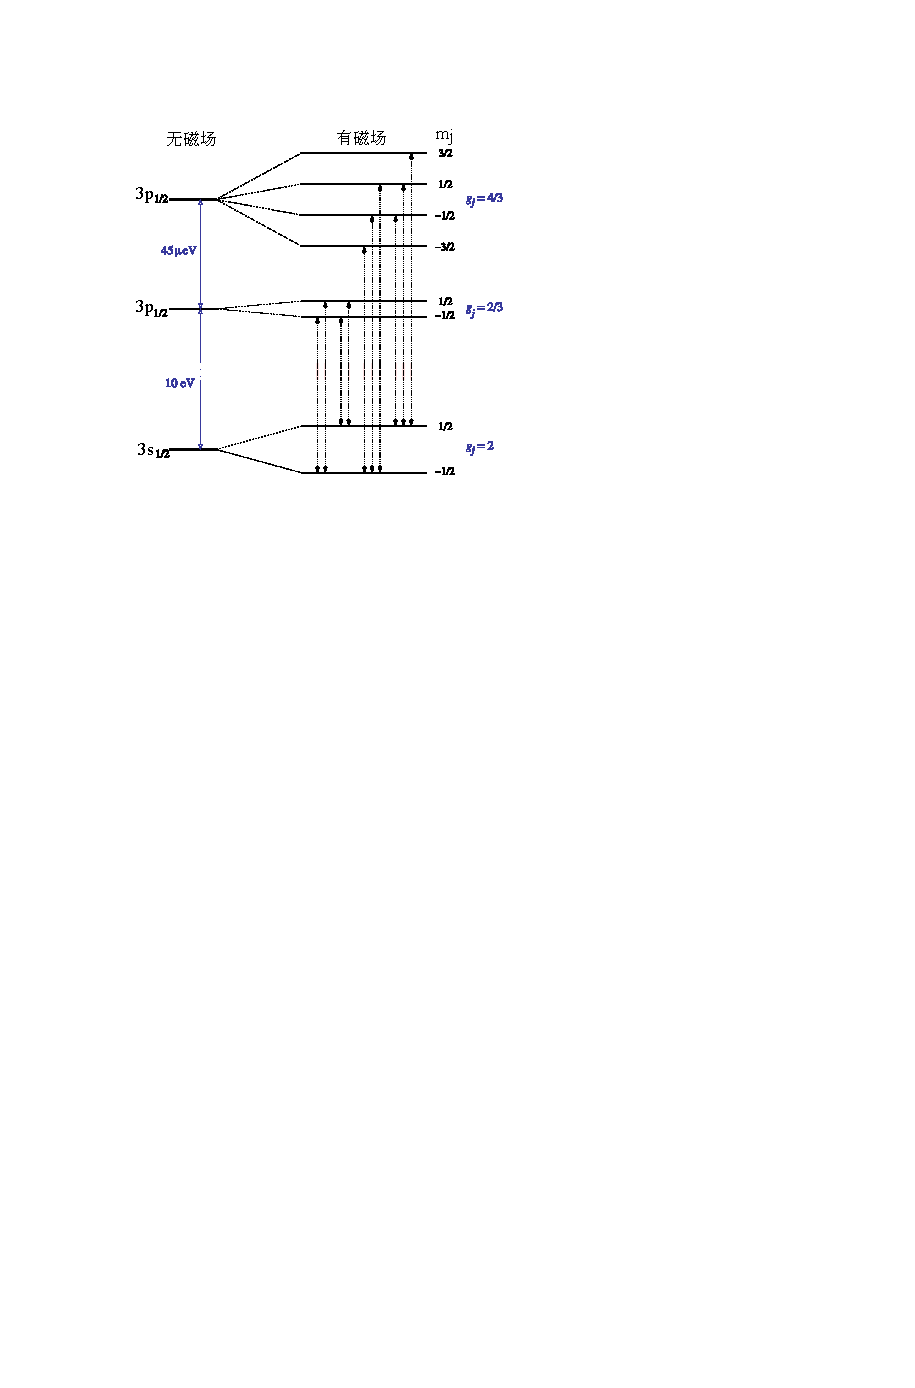
\includegraphics[width=5cm,clip]{QM file/figure/7-3}
	\caption{}\label{fig.7-3}
\end{figure}


\example 证明朗德$g$因子也可以表示成
\eqlong
\begin{empheq}{equation}\label{eq75.16}
	g=1+\frac{j(j+1)+s(s+1)-l(l+1)}{2j(j+1)}\quad \bigg(s=\frac{1}{2}\bigg)
\end{empheq}\eqnormal

\solution 由\eqref{eq72.27}式,可得(以下各式中,$\boldsymbol{\sigma}\cdot\boldsymbol{L}$均指其本征值.$\hbar$均略去不写)
\eqshort
\begin{empheq}{equation}\label{eq75.17}
	\overline{S_{z}}=\frac{m_{j}}{1+2\boldsymbol{\sigma}\cdot\boldsymbol{L}}
\end{empheq}\eqnormal
而\eqref{eq72.5}式取本征值,有
\begin{empheq}{equation}\label{eq75.18}
	j(j+1)=l(l+1)+\frac{3}{4}+\boldsymbol{\sigma}\cdot\boldsymbol{L}
\end{empheq}
利用\eqref{eq72.11}式消去$l(l+1)$,成为
\begin{empheq}{equation}\label{eq75.19}
	\begin{aligned}
		j(j+1)&=(\boldsymbol{\sigma}\cdot\boldsymbol{L})^{2}+2\boldsymbol{\sigma}\cdot\boldsymbol{L}+\frac{3}{4}	\\
		&=\bigg(\boldsymbol{\sigma}\cdot\boldsymbol{L}+\frac{1}{2}\bigg)\bigg(\boldsymbol{\sigma}\cdot\boldsymbol{L}+\frac{3}{2}\bigg)
	\end{aligned}
\end{empheq}
利用此式,可将\eqref{eq75.17}式变成
\begin{empheq}{align}\label{eq75.20}
	\frac{\overline{S_{z}}}{m_{j}} &=\frac{\boldsymbol{\sigma}\cdot\boldsymbol{L}+\frac{3}{2}}{2j(j+1)},\text{再\eqref{eq75.18}利用式,}	\nonumber\\
	&=\frac{j(j+1)+\frac{3}{4}-l(l+1)}{2j(j+1)}
\end{empheq}
再代入\eqref{eq75.13}式,即得
\eqlong
\begin{empheq}{equation*}
	g=1+\frac{\overline{S_{z}}}{m_{j}\hbar}=1+\frac{j(j+1)+\frac{3}{4}-l(l+1)}{2j(j+1)}
\end{empheq}\eqnormal
此即\eqref{eq75.16}式.

% 磁共振
\starthis\section[磁共振]{磁共振} \label{sec:07.06} % 
% \makebox[5em][s]{} % 短题目拉间距

磁共振的基本原理是利用粒子的磁矩在交变磁场中作周期性变化的规律,对磁矩或磁场作精密测量.

以自旋为$\frac{\hbar}{2}$的粒子为例,自旋磁矩算符可以表示成
\eqshort
\begin{empheq}{equation}\label{eq76.1}
	\boldsymbol{\mu}=\mu_{0}\boldsymbol{\sigma}
\end{empheq}\eqnormal
$\boldsymbol{\sigma}$为泡利算符,$\mu_{0}$由粒子性质决定,对于电子,$\mu_{0}=-\frac{e\hbar}{2m_{e}c}$.将粒子置于恒定磁场$B_{0}$中,(以磁场方向为$z$轴方向)则磁作用势(略去与自旋无关的项)为
\begin{empheq}{equation}\label{eq76.2}
	\hat{H}_{0}=-B_{0}\cdot\boldsymbol{\mu}=-B_{0}\mu_{0}\sigma_{z}
\end{empheq}
这时$\sigma_{z}$是守恒量(和$H_{0}$对易),它的本征态$\chi_{1/2}$及$\chi_{-1/2}$也是$H_{0}$的本征态,相应的能级为
\begin{empheq}{equation}\label{eq76.3}
	E_{\pm}=\mp B_{0}\mu_{0}=\mp\hbar\omega,\quad \omega=\frac{B_{0}\mu_{0}}{\hbar}
\end{empheq}
现在再加上一个和$B_{0}$垂直的交变磁场$B_{1}(t)$,
\begin{empheq}{equation}\label{eq76.4}
	B_{1x}=B_{1}\cos\nu t,\quad B_{1y}=-B_{1}\sin\nu t,\quad B_{1z}=0
\end{empheq}
磁作用势变成
\begin{empheq}{align}\label{eq76.5}
	\hat{H} &=-(B_{0}+B_{1})\cdot\boldsymbol{\mu}	\nonumber\\
	&=-B_{0}\mu_{0}\sigma_{z}+B_{1}\mu_{0}(\sigma_{y}\sin\nu t-\sigma_{x}\cos\nu t)
\end{empheq}
如将$H$在$\sigma_{z}$表象中写成矩阵形式,就是
\begin{empheq}{equation*}\label{eq76.5'}
	\hat{H}=-\mu_{0}\begin{bmatrix}
		B_{0} & B_{1}e^{i\nu t}	\\
		B_{1}e^{-i\nu t} & -B_{0} \\
	\end{bmatrix}
\end{empheq}

设在$t=0$时粒子自旋指向$z$方向,即初始自旋波函数为
\eqshort
\begin{empheq}{equation}\label{eq76.6}
	\chi(t=0)=\chi_{1/2}=\begin{bmatrix}
		1 \\  0
	\end{bmatrix}
\end{empheq}
在$t>0$时,由于$B_{1}$场的存在,$\sigma_{z}$不再是守恒量,自旋波函数将按照薛定谔方程
\begin{empheq}{equation}\label{eq76.7}
	i\hbar\frac{d}{dt}\chi(t)=\hat{H}\chi(t)
\end{empheq}\eqnormal
随$t$变化,$\chi(t)$可以表示成
\begin{empheq}{equation}\label{eq76.8}
	\chi(t)=C_{1}(t)\chi_{1/2}+C_{2}(t)\chi_{-1/2}=\begin{bmatrix}
		C_{1}(t)	\\	C_{2}(t)
	\end{bmatrix}
\end{empheq}
将\eqref{eq76.5'}及\eqref{eq76.8}式代入\eqref{eq76.7}式,得到$C_{1},C_{2}$的联立方程
\begin{empheq}{equation}\label{eq76.9}
	{}\begin{dcases}
		i\hbar\dot{C_{1}}=-\mu_{0}B_{0}C_{1}-\mu_{0}B_{1}e^{i\nu t}C_{2}	\\
		i\hbar\dot{C_{2}}=\mu_{0}B_{0}C_{2}-\mu_{0}B_{1}e^{-i\nu t}C_{1}
	\end{dcases}
\end{empheq}
令
\begin{empheq}{equation}\label{eq76.10}
	C_{1}=a(t)e^{i\nu t/2},\quad C_{2}=b(t)e^{-i\nu t/2}
\end{empheq}
可将\eqref{eq76.9}式简化成
\eqlong
\begin{empheq}{equation}\label{eq76.11}
	{}\begin{dcases}
		\dot{a}=i\bigg(\omega-\frac{\nu}{2}\bigg)a+i\gamma\omega b
		\dot{b}=-i\bigg(\omega-\frac{\nu}{2}\bigg)b+i\gamma\omega a
	\end{dcases}\eqnormal
\end{empheq}
其中
\eqshort
\begin{empheq}{equation}\label{eq76.12}
	\omega=\frac{\mu_{0}B_{0}}{\hbar},\quad \gamma=\frac{B_{1}}{B_{0}}
\end{empheq}\eqnormal
实验测量是在“共振条件”$\nu=2\omega$情况下进行,这时\eqref{eq76.11}式成为
\begin{empheq}{equation}\label{eq76.13}
	{}\begin{dcases}
		\dot{a}=i\gamma\omega b
		\dot{b}=i\gamma\omega a
	\end{dcases}\quad (\nu=2\omega)
\end{empheq}
解为
\begin{empheq}{equation*}
	a(t)\pm b(t)=[a(0)\pm b(0)]e^{\pm i\gamma\omega t}
\end{empheq}
根据初始条件\eqref{eq76.6}式,$a(0)=1,b(0)=0$,因此
\eqshort
\begin{empheq}{equation*}
	a(t)\pm b(t)=e^{\pm i\gamma\omega t}
\end{empheq}\eqnormal
解出
\begin{empheq}{equation}\label{eq76.14}
	a(t)=\cos\gamma\omega t,\quad b(t)=i\sin\gamma\omega t
\end{empheq}
代入\eqref{eq76.8}式、\eqref{eq76.10}式,就得到自旋波函数
\begin{empheq}{align}\label{eq76.15}
	\chi(t) &=\cos\gamma\omega e^{i\omega t}\chi_{1/2}+i\sin\gamma\omega t e^{-i\omega t}\chi_{-1/2}	\nonumber\\
	&=\begin{bmatrix}
		\cos\gamma\omega te^{i\omega t}	\\
		i\sin\gamma\omega te^{-i\omega t}
	\end{bmatrix}
\end{empheq}
以$t=0$时粒子的初始自旋方向(正$z$轴方向,$\sigma_{z}=1$)为标准,在时刻$t$自旋方向反转$(\sigma_{z}=-1)$的概率为
\eqshort
\begin{empheq}{equation}\label{eq76.16}
	|C_{2}|^{2}=\sin^{2}\gamma\omega t
\end{empheq}\eqnormal
当$t=\frac{\pi}{2\gamma\omega}=\frac{\pi\hbar}{2\mu_{0}B_{1}}$,粒子自旋方向刚好完全反转.($C_{1}=0$,\eqref{eq76.15}式中只有$\chi_{-1/2}$几项)

在非共振条件下,即$\nu\neq\omega$时,\eqref{eq76.11}式仍存在振动解,令
\begin{empheq}{equation}\label{eq76.17}
	{}\begin{dcases}
		a(t)=a_{1}e^{i\Omega t}+a_{2}e^{-i\Omega t}	\\
		b(t)=b_{1}e^{i\Omega t}+b_{2}e^{-i\Omega t}
	\end{dcases}
\end{empheq}
代入\eqref{eq76.11}式,容易得到存在非平庸解($a_{1},a_{2},b_{1},b_{2}$不全为0)的条件为
\begin{empheq}{equation*}
	\begin{vmatrix}
		\omega+\bigg(\omega-\frac{\nu}{2}\bigg)	& \gamma\omega \\
		\gamma\omega & \Omega-\bigg(\omega-\frac{\nu}{2}\bigg)	
	\end{vmatrix}=0
\end{empheq}
解出
\begin{empheq}{equation}\label{eq76.18}
	\Omega=\bigg[\bigg(\omega-\frac{\nu}{2}\bigg)^{2}+\gamma^{2}\omega^{2}\bigg]^{1/2}
\end{empheq}
考虑到初始条件\eqref{eq76.6}式,即$a(0)=1,b(0)=0$,\eqref{eq76.17}式可以写成
\begin{empheq}{equation*}\label{eq76.17'}
	{}\begin{dcases}
		a(t)=\cos\Omega t+a_{3}\sin\Omega t	\\
		b(t)=b_{3}\sin\Omega t
	\end{dcases}
\end{empheq}
代入\eqref{eq76.11}式,并利用\eqref{eq76.18}式,求出
\begin{empheq}{equation*}
	a_{3}=i\frac{\omega-\frac{\nu}{2}}{\Omega},\quad b_{3}=i\frac{\gamma\omega}{\Omega}
\end{empheq}
\begin{empheq}{equation}\label{eq76.19}
	{}\begin{dcases}
		a(t)=\cos\Omega t+i\frac{\omega-\frac{\nu}{2}}{\Omega}\sin\Omega t	\\
		b(t)=i\frac{\gamma\omega}{\Omega}\sin\Omega t
	\end{dcases}
\end{empheq}
注意,在共振条件$(\nu=2\omega)$下,$\Omega=\gamma\omega$,\eqref{eq76.19}式变成\eqref{eq76.14}式.由\eqref{eq76.8}式、\eqref{eq76.10}式、\eqref{eq76.19}式可知,非共振条件下,时刻$t$自旋方向反转概率
\begin{empheq}{equation}\label{eq76.20}
	|b(t)|^{2}=\bigg(\frac{\gamma\omega}{\Omega}\bigg)^{2}\sin^{2}\Omega t
\end{empheq}
显然
\begin{empheq}{equation}\label{eq76.21}
	|b(t)|_{\text{极大}}^{2}=\bigg(\frac{\gamma\omega}{\Omega}\bigg)^{2}<1
\end{empheq}
而在共振条件下$(\nu=2\omega)$自旋方向反转概率最大可以达到1.

粒子自旋方向的反转,相当于在磁能级$E_{+},E_{-}$间的跃迁,与此相应,粒子从电磁波(交变磁场)中吸收能量
\begin{empheq}{equation}\label{eq76.22}
	\hbar\nu=2\hbar\omega=E_{-}-E_{+}=2B_{0}\mu_{0}
\end{empheq}
在磁共振实验中,交变磁场的频率$\nu$可以调整,当达到共振条件$(\nu=2\omega)$时,出现交变场功率的吸收峰.如$B_{0}$已经精确给定,利用\eqref{eq76.22}式就可测出粒子磁矩$\mu_{0}$.反之,如$\mu_{0}$已知,则可测定$B_{0}$.由于$2\omega$是在射频至微波频段,测量可以达到很高的精度.

对于化合物或凝聚态物质,由于存在自旋轨道耦合作用以及原子间互作用,磁矩结构及磁能级较为复杂,利用磁共振技术可以获得物质结构单元的磁矩信息,有助于了解材料的结构.


% 两个角动量的耦合
\section[两个角动量的耦合]{两个角动量的耦合} \label{sec:07.07} % 
% \makebox[5em][s]{} % 短题目拉间距

电子的自旋角动量与轨道角动量相加成总角动盘($\S$\ref{sec:07.02})是角动量耦合的一个实例.本节讨论一般的角动量耦合问题.

设$\boldsymbol{J}_{1}$和$\boldsymbol{J}_{2}$是属于不同自由度的角动量算符,它们互相对易:
\begin{empheq}{equation}\label{eq77.1}
	[J_{1\alpha},J_{2\beta}]=0,\quad \alpha,\beta = x,y,z
\end{empheq}
而又各自满足角动量对易式:
\begin{empheq}{equation}\label{eq77.2}
	\boldsymbol{J}_{1}\times\boldsymbol{J}_{1}=i\hbar\boldsymbol{J}_{1},\quad \boldsymbol{J}_{2}\times\boldsymbol{J}_{2}=i\hbar\boldsymbol{J}_{2}
\end{empheq}
因此必然有
\begin{empheq}{equation}\label{eq77.3}
	[\boldsymbol{J}_{1}^{2},\boldsymbol{J}_{1}]=0,\quad [\boldsymbol{J}_{2}^{2},\boldsymbol{J}_{2}]=0
\end{empheq}
以$\boldsymbol{J}$表示$\boldsymbol{J}_{1},\boldsymbol{J}_{2}$之和,即
\begin{empheq}{equation}\label{eq77.4}
	\boldsymbol{J}=\boldsymbol{J}_{1}+\boldsymbol{J}_{2}
\end{empheq}
则
\begin{empheq}{equation}\label{eq77.5}
	\boldsymbol{J}^{2}=\boldsymbol{J}_{1}^{2}+\boldsymbol{J}_{2}^{2}+2\boldsymbol{J}_{1}\cdot\boldsymbol{J}_{2}
\end{empheq}
由\eqref{eq77.1}式,易知
\begin{empheq}{align}
	\boldsymbol{J}_{1}\cdot\boldsymbol{J}_{2}&=\boldsymbol{J}_{2}\cdot\boldsymbol{J}_{1}	\label{eq77.6}\\
	\boldsymbol{J}_{1}\times\boldsymbol{J}_{2}&=-\boldsymbol{J}_{2}\times\boldsymbol{J}_{1}	\label{eq77.7}
\end{empheq}
因此
\eqlong
\begin{empheq}{align}\label{eq77.8}
	\boldsymbol{J}\times\boldsymbol{J}&=\boldsymbol{J}_{1}\times\boldsymbol{J}_{1}+\boldsymbol{J}_{2}\times\boldsymbol{J}_{2}+\boldsymbol{J}_{1}\times\boldsymbol{J}_{2}+\boldsymbol{J}_{2}\times\boldsymbol{J}_{1}	\nonumber\\
	&=i\hbar\boldsymbol{J}_{1}+i\hbar\boldsymbol{J}_{2}=i\hbar\boldsymbol{J}
\end{empheq}\eqnormal
因此$\boldsymbol{J}$也是角动量容易证明
\eqshort
\begin{empheq}{equation}\label{eq77.9}
	[\boldsymbol{J}^{2},\boldsymbol{J}]=0
\end{empheq}\eqnormal
利用\eqref{eq77.3}式容易证明
\begin{empheq}{equation}\label{eq77.10}
	[\boldsymbol{J}_{1}^{2},\boldsymbol{J}]=0,\quad [\boldsymbol{J}_{2}^{2},\boldsymbol{J}]=0
\end{empheq}
因此,$\boldsymbol{J}_{1}^{2},\boldsymbol{J}_{2}^{2},\boldsymbol{J}^{2},J_{z}$互相对易,可以选作力学量完全集.
\pskip

$\S$\ref{sec:04.07}中关于角动量的一般理论对于这里的$\boldsymbol{J}_{1},\boldsymbol{J}_{2}$和$\boldsymbol{J}$均可适用.以$\varPsi_{j_{1}m_{1}}$或$|j_{1}m_{1}\rangle$表示$(\boldsymbol{J}_{1}^{2},J_{1z})$共同本征态,即设
\eqlong
\begin{empheq}{equation}\label{eq77.11}
	\begin{aligned}
		\boldsymbol{J}_{1}^{2}\varPsi_{j_{1}m_{1}} &=j_{1}(j+1)\hbar^{2}\varPsi_{j_{1}m_{1}}	\\
		J_{1z}\varPsi_{j_{1}m_{1}} &=m_{1}\hbar\varPsi_{j_{1}m_{1}},\quad m_{1}=j_{1},j_{1}-1,\cdots(-j_{1})
	\end{aligned}
\end{empheq}
按照$\S$\ref{sec:04.07},升降算符的作用结果是
\eqllong
\begin{empheq}{equation}\label{eq77.12}
	(J_{1x}\pm iJ_{1y})\varPsi_{j_{1}m_{1}}=\hbar\sqrt{(j_{1}\pm m_{1}+1)(j_{1}\mp m_{1})}\varPsi_{j_{1}m_{1}\pm 1}
\end{empheq}
类似地,以$\varPsi_{j_{2}m_{2}}$或$|j_{2}m_{2}\rangle$表示$(\boldsymbol{J}_{2}^{2},J_{2z})$共同本征态,也有类似于\eqref{eq77.11}式、\eqref{eq77.12}式的公式,不再一一写出.
\pskip

$(\boldsymbol{J}_{1}^{2},\boldsymbol{J}_{2}^{2},\boldsymbol{J}^{2},J_{z})$共同本征态记为$\varPsi_{j_{1}j_{2}jM}$或$|j_{1}j_{2}jM\rangle$,相应于本征值
\begin{empheq}{equation}\label{eq77.13}
	\begin{aligned}
		&\boldsymbol{J}_{1}^{2}=j_{1}(j_{1}+1)\hbar^{2},\quad &\boldsymbol{J}_{2}^{2}=j_{2}(j_{2}+1)\hbar^{2}			\\
		&\boldsymbol{J}^{2}=j(j+1)\hbar^{2},\quad 
		&J_{z}=M\hbar,M=j,j-1,\cdots,(-j)
	\end{aligned}
\end{empheq}\eqlong
首先要解决的问题是,当$j_{1}$与$j_{2}$给定后,$j$有哪些可能取值.其次的问题是,$\varPsi_{j_{1}j_{2}jM}$态和$\varPsi_{j_{1}m_{1}}$及$\varPsi_{j_{2}m_{2}}$态是什么关系.按照$\S$\ref{sec:07.02}的经验,$\varPsi_{j_{1}j_{2}jM}$显然可以表示成
\begin{empheq}{equation}\label{eq77.14}
	\varPsi_{j_{1}j_{2}jM}=\sum_{m_{1}}\sum_{m_{2}}C(j,M,m_{1},m_{2})\varPsi_{j_{1}m_{1}}\varPsi_{j_{2}m_{2}}
\end{empheq}\eqnormal
由于$J_{z}=J_{1z}+J_{2z}$,显然有
\begin{empheq}{equation}\label{eq77.15}
	J_{z}\varPsi_{j_{1}m_{1}}\varPsi_{j_{2}m_{2}}=(m_{1}+m_{2})\hbar\varPsi_{j_{1}m_{1}}\varPsi_{j_{2}m_{2}}
\end{empheq}
因此\eqref{eq77.14}式中只包含$m_{1}+m_{2}=M$的项.给定$j_{1},j_{2}$后,$m_{1}$共有$(2j_{1}+1)$种取值(依次相差1),$m_{2}$共有$(2j_{2}+1)$种取值(依次相差1),故\eqref{eq77.14}式右端最多有$(2j_{1}+1)(2j_{2}+1)$种独立项,最多能组成同样数目的独立的$\varPsi_{j_{1}j_{2}jM}$.其中对于某个$j$值,相应的$M$值有$(2j+1)$种,即
\begin{empheq}{equation*}
	M=j,j-1,\cdots,(-j)
\end{empheq}
由于$M$值只能依次相差1,所以$j$也只能依次相差1.$M$的最大值显然是$(j_{1}+j_{2})$,这也就是$j$的最大值.因此,$j$的可能取值为
\begin{empheq}{equation*}
	j=j_{1}+j_{2},j_{1}+j_{2}-1,\cdots,j_{min}
\end{empheq}
由此可知,独立的$\varPsi_{j_{1}j_{2}jM}$总数为
\begin{empheq}{equation*}
	N=\sum_{j}(2j+1)=(j_{1}+j_{2}+j_{min}+1)(j_{1}+j_{2}-j_{min}+1)
\end{empheq}
上式应等于$(2j_{1}+1)(2j_{2}+1)$,为此必须$j_{min}=|j_{1}-j_{2}|$.因此,$j$的取值为
\begin{empheq}{equation}\label{eq77.16}
	\boxed{j=j_{1}+j_{2},j_{1}+j_{2}-1,\cdots,|j_{1}-j_{2}|}
\end{empheq}
量子数$j_{1},j_{2}$,$j$之间的这种关系常被形象地称为三角形条件,记为$\Delta(j_{1}j_{2}j)$,或用图\ref{fig.7-4}表示,但必须记住,$j$是量子化的,所以图中$j_{1},j_{2}$的夹角也必须是量子化的,以保证\eqref{eq77.16}式成立.

\begin{wrapfigure}[8]{r}{7em}
	\centering
	\small
	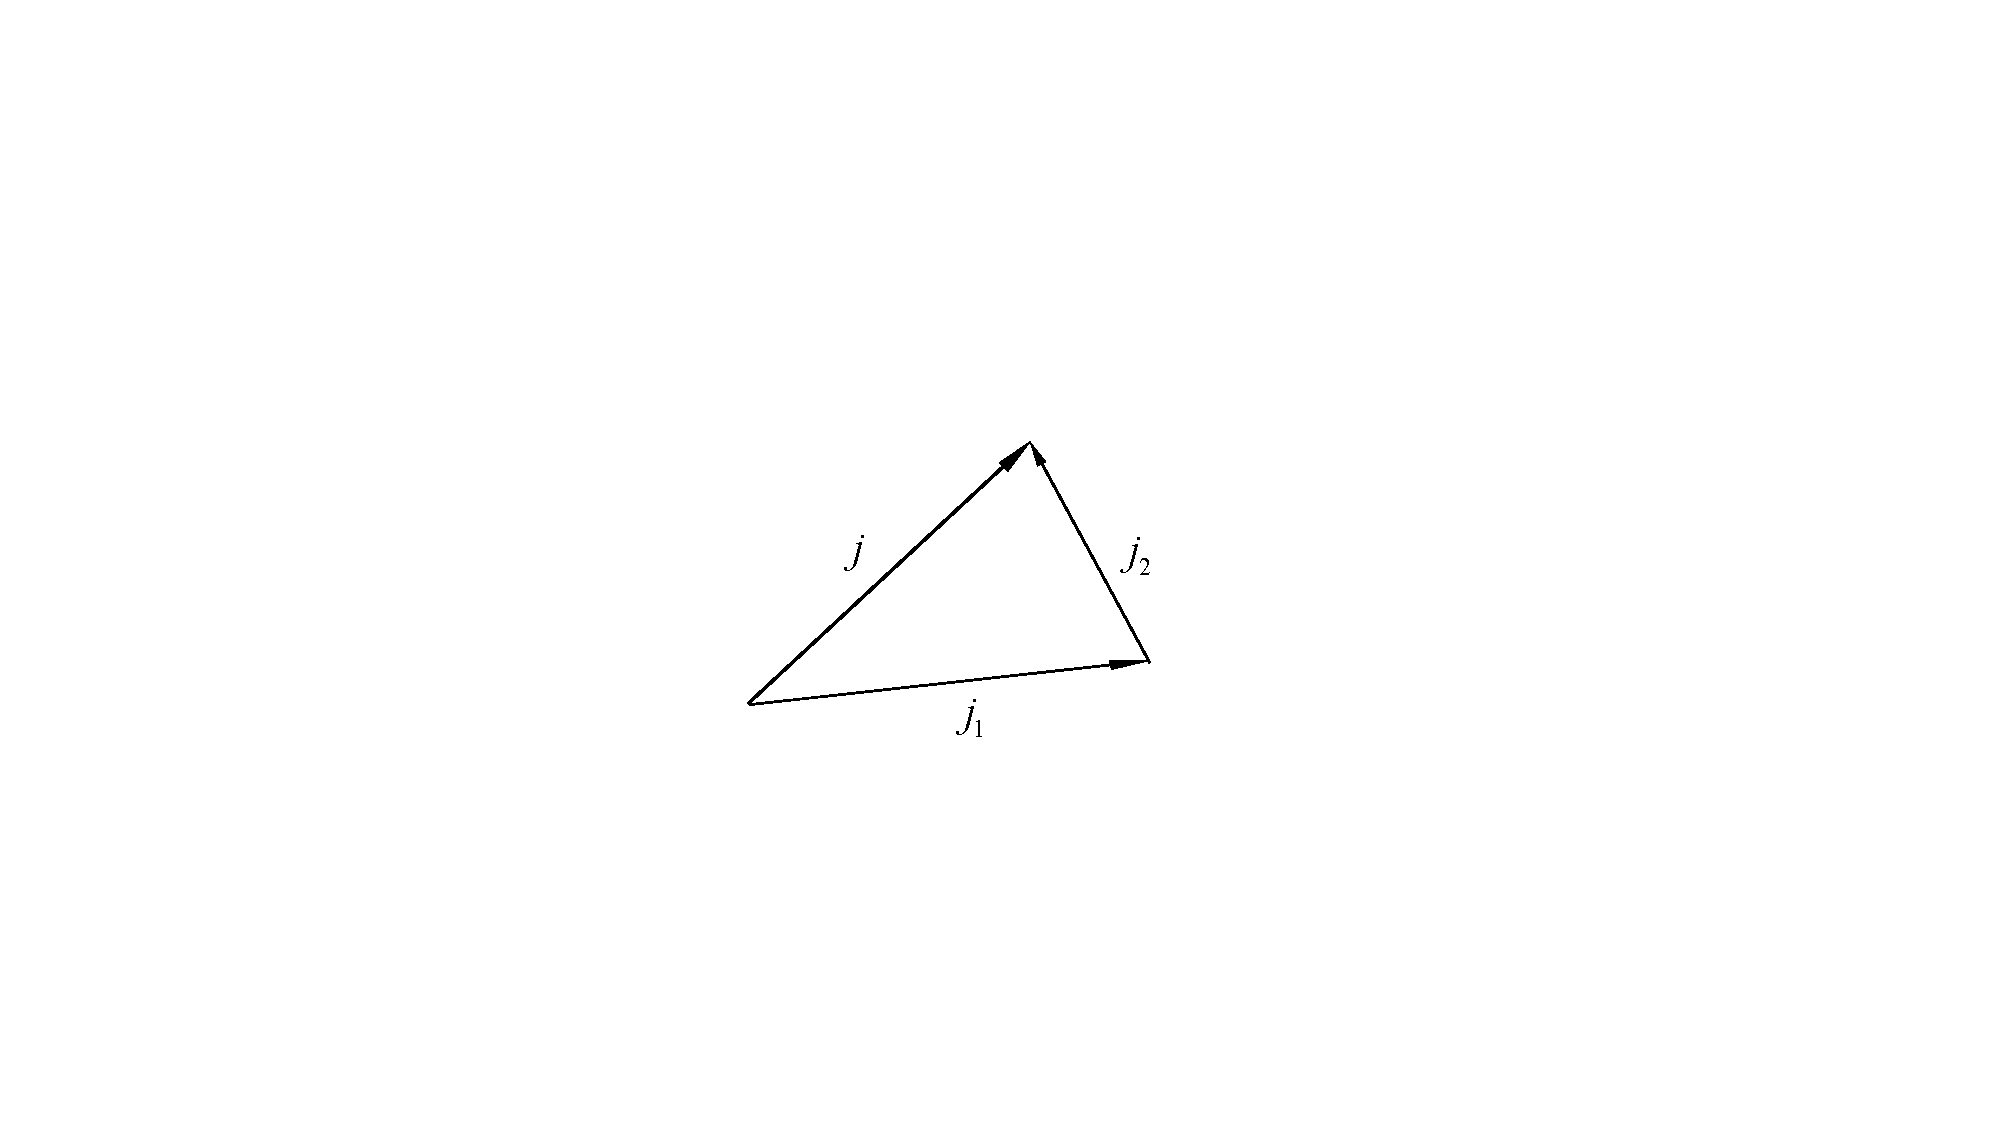
\includegraphics[width=3cm,clip]{QM file/figure/7-4}
	\caption{}\label{fig.7-4}
\end{wrapfigure}

\eqref{eq77.14}式中的系数$C(j,M,m_{1},m_{2})$称为C.G.(Clebsch-Gordan)系数,也称矢耦系数,有关理论和公式相当复杂,从略.如采用狄拉克态矢量符号,$\varPsi_{j_{1}m_{1}},\varPsi_{j_{2}m_{2}}$记成$|j_{1}m_{1},j_{2}m_{2}\rangle$,$\varPsi_{j_{1}j_{2}jM}$记成$|j_{1}j_{2}jM\rangle$,简写成$|jM\rangle$.给定$j_{1},j_{2}$后,我们就有一个$(2j_{1}+1)(2j_{2}+1)$维态矢量空间.如以$|j_{1}m_{1},j_{2}m_{2}\rangle$作为基矢,相应的表象称为非耦合表象;如以$|jM\rangle$作为基矢,相应的表象称为耦合表象.利用恒等变换公式
\begin{empheq}{equation}\label{eq77.17}
	\sum_{m_{1}}\sum_{m_{2}}|j_{1}m_{1},j_{2}m_{2}\rangle \langle j_{1}m_{1},j_{2}m_{2}|=1
\end{empheq}
将$|jM\rangle$在非耦合表象中展开成
\begin{empheq}{equation}\label{eq77.18}
	|jM\rangle=\sum_{m_{1}}\sum_{m_{2}}|j_{1}m_{1},j_{2}m_{2}\rangle \langle j_{1}m_{1},j_{2}m_{2}|jM\rangle 
\end{empheq}
与\eqref{eq77.14}式比较,易见
\begin{empheq}{equation}\label{eq77.19}
	C(jM,m_{1}m_{2})=\langle j_{1}m_{1}j_{2}m_{2}|jM \rangle 
\end{empheq}
显然C.G.系数就是联系两种表象的么正矩阵的矩阵元.

C.G.系数应用极广,有许多类型的C.G.系数表可供查阅.$j_{2}=\frac{1}{2}$和1时C.G.系数如表\ref{lab.7-1},表\ref{lab.7-2}所示.请将$\S$\ref{sec:07.02}中结果与表\ref{lab.7-1}对照$\bigg(j_{1}=l,j_{2}=\frac{1}{2},M=m+\frac{1}{2}\bigg)$


\begin{table}[!h]
	\begin{center}
		\caption{C.G.系数$\langle j_{1}m_{1}j_{2}m_{2}|jM\rangle\bigg(j_{2}=\dfrac{1}{2},m_{1}=M-m_{2}\bigg)$}
		\label{lab.7-1}
		\setlength{\tabcolsep}{8mm}	% 调节表格尺寸
		%\resizebox{h-length}{v-length}{text}
		\begin{tabular}{c|c|c}
			\toprule[1pt]
			\multirow{2}{*}{	} & \multirow{2}{*}{$m_{2}=\frac{1}{2}$} & \multirow{2}{*}{$m_{2}=-\frac{1}{2}$}	\\ 
			 & & \\
			\hline
			\multirow{2}{*}{}
			\multirow{2}{*}{$j=j_{1}+\frac{1}{2}$} & \multirow{2}{*}{$\sqrt{\frac{j_{1}+M+\frac{1}{2}}{2j_{1}+1}}$} & \multirow{2}{*}{$\sqrt{\frac{j_{1}-M+\frac{1}{2}}{2j_{1}+1}}$}	\\ 
			& & \\
			\hline
			\multirow{2}{*}{$j=j_{1}-\frac{1}{2}$} & \multirow{2}{*}{$-\sqrt{\frac{j_{1}-M+\frac{1}{2}}{2j_{1}+1}}$} & \multirow{2}{*}{$\sqrt{\frac{j_{1}+M+\frac{1}{2}}{2j_{1}+1}}$}	\\ 
			& & \\
			\bottomrule[1pt]
		\end{tabular}
	\end{center}
\end{table}

\begin{table}[!h]
	\begin{center}
		\caption{C.G.系数$\langle j_{1}m_{1}j_{2}m_{2}|jM\rangle\bigg(j_{2}=1,m_{1}=M-m_{2}\bigg)$}
		\label{lab.7-2}
		%\setlength{\tabcolsep}{3mm}	% 调节表格尺寸
		%\resizebox{h-length}{v-length}{text}
		\begin{tabular}{c|c|c|c}
			\toprule[1pt]
			\multirow{2}{*}{	}& \multirow{2}{*}{$m_{2}=1$} & \multirow{2}{*}{$m_{2}=0$} & \multirow{2}{*}{$m_{2}=-1$}	\\
			 & & & \\
			\hline
			\multirow{2}{*}{$j=j_{1}+1$} & \multirow{2}{*}{$\sqrt{\frac{(j_{1}+M)(j_{1}+M+1)}{(2j_{1}+1)(2j_{1}+2)}}$} & \multirow{2}{*}{$\sqrt{\frac{(j_{1}-M+1)(j_{1}+M+1)}{(j_{1}+1)(2j_{1}+1)}}$} 	& \multirow{2}{*}{$\sqrt{\frac{(j_{1}-M)(j_{1}-M+1)}{(2j_{1}+1)(2j_{1}+2)}}$}	\\
			 & & & \\
			\hline
			\multirow{2}{*}{$j=j_{1}$} & \multirow{2}{*}{$-\sqrt{\frac{(j_{1}+M)(j_{1}-M+1)}{2j_{1}(j_{1}+1)}}$} & \multirow{2}{*}{$\sqrt{\frac{M}{j_{1}(j_{1}+1)}}$} 	& \multirow{2}{*}{$\sqrt{\frac{(j_{1}-M)(j_{1}+M+1)}{2j_{1}(j_{1}+1)}}$}	\\
			 & & & \\
			\hline
			\multirow{2}{*}{$j=j_{1}-1$} & \multirow{2}{*}{$\sqrt{\frac{(j_{1}-M)(j_{1}-M+1)}{2j_{1}(2j_{1}+1)}}$} & \multirow{2}{*}{$-\sqrt{\frac{(j_{1}-M)(j_{1}+M)}{j_{1}(2j_{1}+1)}}$} 	& \multirow{2}{*}{$\sqrt{\frac{(j_{1}+M+1)(j_{1}+M)}{2j_{1}(2j_{1}+1)}}$}	\\
			 & & & \\
			\bottomrule[1pt]
		\end{tabular}
	\end{center}
\end{table}

\newpage







% 二电子体系的自旋波函数
\section[二电子体系的自旋波函数]{二电子体系的自旋波函数} \label{sec:07.08} % 


以$\boldsymbol{S}_{1}$和$\boldsymbol{S}_{2}$表示电子1和2的自旋角动量,体系的总自旋为
\eqshort
\begin{empheq}{equation}\label{eq78.1}
	\boldsymbol{S}=\boldsymbol{S}_{1}+\boldsymbol{S}_{2}
\end{empheq}
其分量为
\begin{empheq}{equation}\label{eq78.2}
	S_{z}=S_{1z}+S_{2z}
\end{empheq}\eqnormal
等等总自旋平方为
\begin{empheq}{equation}\label{eq78.3}
	\boldsymbol{S}^{2}=\boldsymbol{S}_{1}^{2}+\boldsymbol{S}_{2}^{2}+2\boldsymbol{S}_{1}\cdot\boldsymbol{S}_{2}
\end{empheq}
根据实验事实,
\eqshort
\begin{empheq}{equation}\label{eq78.4}
	\boldsymbol{S}_{1}^{2}=\boldsymbol{S}_{2}^{2}=\frac{3}{4}\hbar^{2}
\end{empheq}\eqnormal
这相当于$j_{1}=j_{2}=\frac{1}{2}$的情形.$\boldsymbol{S}^{2}$及$S_{z}$的本征值记为
\begin{empheq}{equation*}
	\boldsymbol{S}^{2}——S(S+1)\hbar^{2},\quad S_{z}--M_{s}\hbar
\end{empheq}
按照角动量耦合理论,总自旋量子数$S$的可能取值为1和0,$M_{s}$的取值为
\begin{empheq}{equation}\label{eq78.5}
	\boxed{\begin{aligned}
		S=1, &&M_{s}=1,0,-1	\\
		S=0, &&M_{s}=0
	\end{aligned}}
\end{empheq}
现在还需要确定$\boldsymbol{S}^{2},S_{z}$的共同本征态.

电子$1,2$各有两种独立自旋态$\chi_{1/2}$,$\chi_{-1/2}$,在这里记为$\alpha,\beta$.非耦合表象中的基矢$|j_{1}m_{1},j_{2}m_{2}\rangle$共有4个,它们是
\begin{empheq}{equation}\label{eq78.6}
	\alpha(1)\alpha(2),\alpha(1)\beta(2),\beta(1)\alpha(2),\beta(1)\beta(2)
\end{empheq}
它们都是总$S_{z}$的本征态,$M_{s}$依次为$1,0,0,-1$.按照\eqref{eq78.5}式,$M_{s}$等于1和-1时,$S$必然为1.因此可以判断$\alpha(1)\alpha(2)$和$\beta(1)\beta(2)$都已经是$\boldsymbol{S}^{2},S_{z}$的共同本征态$|S,M_{S}\rangle$,在这里记成$\chi_{SM_{S}}$,即
\begin{empheq}{equation}\label{eq78.7}
	\chi_{11}=\alpha(1)\alpha(2),\quad \chi_{1-1}=\beta(1)\beta(2)
\end{empheq}
$S=1$时,$\boldsymbol{S}^{2},S_{z}$还有一个共同本征态$(M_{S}=0)$,它应该由\eqref{eq78.6}式中第二、三项叠加而成.按照角动量一般理论[\eqref{eq47.26}式]
\begin{empheq}{equation}\label{eq78.8}
	(S_{x}-iS_{y})\chi_{11}=\sqrt{2}\hbar\chi_{10}
\end{empheq}
其中$(S_{x}-iS_{y})=(S_{1x}-iS_{1y})+(S_{2x}-iS_{2y})$.利用\eqref{eq71.19}式容易算出
\begin{empheq}{equation*}
	(S_{x}-iS_{y})\chi_{11}=\hbar\alpha(1)\beta(2)+\hbar\beta(1)\alpha(2)
\end{empheq}
代入\eqref{eq78.8}式,即得
\begin{empheq}{equation}\label{eq78.9}
	\chi_{10}=\frac{1}{\sqrt{2}}[\alpha(1)\beta(2)+\beta(1)\alpha(2)]
\end{empheq}
按照角动量一般理论,$\chi_{10}$与$\chi_{1-1}$有关系
\begin{empheq}{equation}\label{eq78.10}
	(S_{x}-iS_{y})\chi_{10}=\sqrt{2}\hbar\chi_{1-1}
\end{empheq}
请读者自行验证.

$\boldsymbol{S}^{2},S_{z}$还有一个共同本征态$\chi_{00}(S=0,M_{S}=0)$,它应该由\eqref{eq78.6}式中第二、三项叠加而成,并与$\chi_{10}$正交(因为量子数$S$之值不同),设
\begin{empheq}{equation*}
	\chi_{00}=C_{1}\alpha(1)\beta(2)+C_{2}\beta(1)\alpha(2)
\end{empheq}
由正交条件
\eqshort
\begin{empheq}{equation*}
	\chi_{10}^{+}\chi_{00}=0
\end{empheq}\eqnormal
容易得出$C_{2}=-C_{1}$.取$C_{1}>0$.并将$\chi_{00}$归一化,最后得到
\begin{empheq}{equation}\label{eq78.11}
	\chi_{00}=\frac{1}{\sqrt{2}}[\alpha(1)\beta(2)-\beta(1)\alpha(2)]
\end{empheq}
利用\eqref{eq71.17}式容易验证$S_{\chi_{00}},S_{\chi_{00}}^{2}=0$.

总结以上计算,我们已经求出二电子体系总自旋平方$\boldsymbol{S}^{2}$和$S_{z}$的全部共同本征函数$\chi_{SM_{S}}$,它们是
\begin{empheq}{equation}\label{eq78.12}
	\begin{aligned}
		\chi_{11} &=\alpha(1)\alpha(2)	\\
		\chi_{10} &=\frac{1}{\sqrt{2}}[\alpha(1)\beta(2)+\beta(1)\alpha(2)]	\\
		\chi_{1-1}&=\beta(1)\beta(2)	\\
		\chi_{00} &=\frac{1}{\sqrt{2}}[\alpha(1)\beta(2)-\beta(1)\alpha(2)]
	\end{aligned}
\end{empheq}
容易验证,它们和表\ref{lab.7-1}列出的C.G.系数是一致的.\eqref{eq78.12}式适用于任何由两个自旋$\frac{1}{2}$粒子组成的体系,应用极广,读者应该牢记.

作为二粒子体系自旋自由度的波函数,\eqref{eq78.6}式4个波函数都能够表示成单粒子波函数的乘积,称为“分离态”.反之,\eqref{eq78.9}式和\eqref{eq78.11}式则为“纠缠态”.近年来由于量子信息论的迅速发展,纠缠态日益引人注目.对于本节讨论的自旋波函数,典型的纠缠态除$\chi_{10}$、$\chi_{00}$外,还有
\begin{empheq}{equation}\label{eq78.13}
	\frac{1}{\sqrt{2}}[\alpha(1)\alpha(2)\pm\beta(1)\beta(2)]
\end{empheq}
它们都是$\sigma_{1x},\sigma_{2x},\sigma_{1z},\sigma_{2z}$的共同本征函数.








% 习题
\begin{exercises}
	
\exercise $n\times n$矩阵$M$的“迹”定义为$\tr M=\sum_{k=1}^{n}M_{kk}$,即对角矩阵元之和证明:任意2阶矩阵$M$可以表示成泡利矩阵$\sigma_{x},\sigma_{y},\sigma_{z}$与单位矩阵$I$的线性叠加,如下式:
\eqlong
\begin{empheq}{align*}
	M &=\frac{1}{2}(\tr M)I+\frac{1}{2}(\tr\boldsymbol{\sigma}M)\cdot\boldsymbol{\sigma}	\\
	&= \frac{1}{2} \{(\tr M)I+(\tr\sigma_{x}M)\sigma_{x}+(\tr\sigma_{y}M)\sigma_{y}+(\tr\sigma_{z}M)\sigma_{z}\}
\end{empheq}\eqnormal
 
\exercise 在$S_{z}$表象中,求$\sigma_{x}$的本征函数及$\sigma_{y}$的本征函数.
 	
\exercise 在$S_{z}$表象中,求$\sigma_{n}$的矩阵表示及其本征函数.$\sigma_{n}=\boldsymbol{n}\cdot\boldsymbol{\sigma}$,$\boldsymbol{n}$为任意$(\theta,\varphi)$方向单位矢量.
 	
\exercise 对于上题求得两个$\sigma_{n}$本征函数,计算$\langle\boldsymbol{\sigma}\rangle$,并求$\Delta S_{x},\Delta S_{y},\Delta S_{z}$,验证不确定关系.
 	
\exercise 证明$(\sigma_{x}+i\sigma_{y})^{2}=0,(\sigma_{x}-i\sigma_{y})^{2}=0$.用$(\sigma_{x}\pm i\sigma_{y})$的矩阵表示($S_{z}$表象)验证这两个公式.
 	
\exercise 讨论下列算符是否存在.如存在,将其表示成$I,\sigma_{x},\sigma_{y},\sigma_{z}$的线性叠加.

(a)$(1+\sigma_{x})^{\frac{1}{2}}$\quad(b)$(1+\sigma_{x}+i\sigma_{y})^{\frac{1}{2}}$\quad (c)$(1+\sigma_{z})^{-1}$
 
\exercise 证明公式$e^{i\lambda\sigma_{z}}=\cos\lambda+i\sigma_{z}\sin\lambda$.($\lambda$为实参数,$\sigma_{z}$为算符)并在$S_{z}$表象中证明
\begin{empheq}{equation*}
	e^{i\lambda\sigma_{z}}=\begin{bmatrix}
		e^{i\lambda} & 0 	\\
		0 & e^{-i\lambda}	\\
	\end{bmatrix}
\end{empheq}
 
\exercise 设$\boldsymbol{A}$为常数矢量,令$\boldsymbol{A}\cdot\boldsymbol{\sigma}=A\sigma_{A}$.证明
\begin{empheq}{equation*}
	e^{i\boldsymbol{A}\cdot\boldsymbol{\sigma}}=\cos A+i\sigma_{A}\sin A
\end{empheq}
 	
\exercise 设$\boldsymbol{A},\boldsymbol{B},\boldsymbol{C}$为常数矢量,求$\tr(\boldsymbol{A}\cdot\boldsymbol{\sigma}),\tr[(\boldsymbol{A}\cdot\boldsymbol{\sigma})(\boldsymbol{B}\cdot\boldsymbol{\sigma})]$及$\tr[(\boldsymbol{A}\cdot\boldsymbol{\sigma})(\boldsymbol{B}\cdot\boldsymbol{\sigma})(\boldsymbol{C}\cdot\boldsymbol{\sigma})]$.
 	
\exercise 证明$\tr(e^{i\boldsymbol{A}\cdot\boldsymbol{\sigma}})=2\cos A$,$\tr(e^{i\lambda\sigma_{x}} e^{i\lambda\sigma_{y}}=2\cos^{2}A)$.
 	
\exercise 证明(a) $\sigma_{z}(\sigma_{x}\pm i\sigma_{y})=(\sigma_{x}\pm i\sigma_{y})(\sigma_{z}\pm 2)$

(b) $f(\sigma_{z})(\sigma_{x}\pm i\sigma_{y})=(\sigma_{x}\pm i\sigma_{y})f(\sigma_{z}\pm 2)$

(c) $e^{i\lambda\sigma_{z}}(\sigma_{x}\pm i\sigma_{y})=e^{\pm2i\lambda}(\sigma_{x}\pm i\sigma_{y})e^{i\lambda\sigma_{z}}$
 	
\exercise 证明$e^{i\lambda\sigma_{z}}\sigma_{x}e^{-i\lambda\sigma_{z}}=\sigma_{x}\cos2\lambda-\sigma_{y}\sin2\lambda$

$e^{i\lambda\sigma_{z}}\sigma_{y}e^{-i\lambda\sigma_{z}}=\sigma_{x}\sin2\lambda+\sigma_{y}\cos2\lambda$
 	
\exercise 令$\hbar=1$,对于电子,证明
\eqlong
\begin{empheq}{equation*}
	(2\boldsymbol{S}\cdot\boldsymbol{L}+1)^{2}=\boldsymbol{J}^{2}+\frac{1}{4},\quad (\boldsymbol{\sigma}\cdot\boldsymbol{J})(\boldsymbol{\sigma}\cdot\boldsymbol{J}-1)=\boldsymbol{J}^{2}
\end{empheq}\eqnormal
 	
\exercise 对于电子的$(\boldsymbol{L}^{2},\boldsymbol{J}^{2},J_{z})$共同本征态$\varPsi_{ljm_{j}}$,对于属于同一个$l$值的那些状态,定义算符
\begin{empheq}{equation*}
	\Lambda_{l}^{+}=\frac{1}{2l+1}(l+1+\boldsymbol{\sigma}\cdot\boldsymbol{L}),\quad \Lambda_{l}^{-}=\frac{1}{2l+1}(l-\boldsymbol{\sigma}\cdot\boldsymbol{L})
\end{empheq}
试确定它们对$\varPsi_{ljm_{j}}$的作用规则,并找出它们满足的基本代数关系.
 	
\exercise  (a) 证明$\sigma_{r}=\dfrac{\boldsymbol{\sigma}\cdot\boldsymbol{r}}{r}$与$\boldsymbol{J}$的各分量对易,即$[\sigma_{r},\boldsymbol{J}]=0$

(b) 对于$\varPsi_{ljm_{j}}$,将$l=j-\dfrac{1}{2}$者记为$\phi_{jm_{j}}^{A}$,$l=j+\dfrac{1}{2}$者记为$\phi_{jm_{j}}^{B}$,证明
\begin{empheq}{equation*}
	\sigma_{r}\phi_{jm_{j}}^{A}=-\phi_{jm_{j}}^{B},\quad \sigma_{r}\phi_{jm_{j}}^{B}=-\phi_{jm_{j}}^{A}
\end{empheq}
并加以解释.

[提示:利用附录\ref{A04}\eqref{eqA4.45}式、\eqref{eqA4.46}式,并注意问题的宇称性]

 	
\exercise 电子的总磁矩算符是
\begin{empheq}{equation*}
	\boldsymbol{\mu}=\boldsymbol{\mu}_{L}+\boldsymbol{\mu}_{s}=-\dfrac{e}{2m_{e}c}(\boldsymbol{L}+2\boldsymbol{S})
\end{empheq}
试对于$\varPsi_{ljj}$态$(m_{j}=j)$计算$\mu_{z}$平均值(结果用量子数$j$表示).
 
\exercise 某电子态波函数为$\Psi(r,\theta,\varphi,S_{z})=R(r)Y_{l0}(\theta,\varphi)\chi_{1/2}(S_{z})$.这是否$\boldsymbol{J}^{2}$或$J_{z}$本征函数?试计算$\langle\boldsymbol{J}^{2}\rangle$,从而求出$\boldsymbol{J}^{2}$的可能测值及相应概率.
 	
\exercise 自旋为0的带电粒子在均匀磁场中运动,哈密顿算符为
\begin{empheq}{equation*}
	\hat{H}=\frac{m}{2}\hat{\boldsymbol{v}}^{2}=\frac{1}{2m}\bigg(\hat{\boldsymbol{p}}-\frac{q}{c}\boldsymbol{A}\bigg)^{2}
\end{empheq}

设磁场沿$z$轴方向,矢势取为$\boldsymbol{A}=\dfrac{1}{2}\boldsymbol{B}\times\boldsymbol{r}$,即
\begin{empheq}{equation*}
	A_{x}=-\frac{By}{2},\quad A_{y}=\frac{Bx}{2},\quad A_{z}=0
\end{empheq}

(a) 计算$v_{x},v_{y},v_{z}$之间的对易式

(b) 设粒子电荷$q>0$.证明$\hat{H}$可以表示成
\begin{empheq}{equation*}
	\hat{H}=\frac{\hbar qB}{2mc}(\hat{Q}^{2}+\hat{P}^{2})+\frac{1}{2m}\hat{p}_{z}^{2}
\end{empheq}
确定$\hat{Q},\hat{P}$,证明$\hat{Q}\hat{P}-\hat{P}\hat{Q}$.

(c) 利用谐振子的结果,确定本题的能谱.
 	
\exercise 将上题的$\hat{H}$表示成\eqref{eq74.7'}式的形式,找出主要的守恒力学量,再找出能级公式.(质量$m$改为$\mu$,以免与量子数混淆.)
 	
\exercise 有一个定域电子(不考虑“轨道”运动),受到沿正$x$方向的均匀磁场作用,磁作用势为
\begin{empheq}{equation*}
	H=\frac{eB}{m_{e}c}S_{x}=\frac{e\hbar B}{2m_{e}c}\sigma_{x}
\end{empheq}
设$t=0$时电子的自旋状态为$\sigma_{z}=1$的本征态,即$\chi_{1/2}=\left[\begin{smallmatrix}
	1 \\ 0 
\end{smallmatrix}\right]$.求任意$t>0$时自旋波函数$\chi(t)=\left[\begin{matrix}
	a(t)	\\	b(t)
\end{matrix}\right]$,并求$\overline{S_{x}}(t),\overline{S_{y}}(t),\overline{S_{z}}(t)$.
 
\exercise 用海森伯运动方程处理上题,求$\overline{S_{x}}(t),\overline{S_{y}}(t),\overline{S_{z}}(t)$.注意先确定$t=0$时它们的初始值.
 	
\exercise 对于氢原子,求自旋轨道耦合作用引起的能级分裂$\Delta E_{nl}$[\eqref{eq73.15}式、\eqref{eq73.12}式]

[提示:$\langle r^{-3}\rangle$利用5-15题结果.]
 
\exercise 设氢原子中电子处于s态$(l=0)$,考虑电子与质子的自旋角动量,$S_{1}$与$S_{2}$.设电子自旋态为$\alpha$,质子自旋态为$\beta$,即总自旋态为$\alpha(1)\beta(2)$.求总自旋平方$\boldsymbol{S}^{2}=(\boldsymbol{S}_{1}+\boldsymbol{S}_{2})^{2}$的可能取值及相应概率.
 	
\exercise 同上题,如电子处于$S_{1z}=\dfrac{\hbar}{2}$的状态(即$\chi_{1/2}$),质子处于$S_{2x}=\dfrac{\hbar}{2}$的状态,求总自旋平方$\boldsymbol{S}^{2}$及总$S_{z}=S_{1z}+S_{2z}$的可能取值及相应概率.
 	
\exercise 考虑由3个自旋$\dfrac{1}{2}$的可分辨粒子组成的体系.

(a) 求总自旋平方$\boldsymbol{S}^{2}=(\boldsymbol{S}_{1}+\boldsymbol{S}_{2}+\boldsymbol{S}_{3})^{2}$的本征值.

(b) 设体系能量算符(略去“轨道”运动)为
\begin{empheq}{equation*}
	H=(\boldsymbol{S}_{1}\cdot\boldsymbol{S}_{2}+\boldsymbol{S}_{2}\cdot\boldsymbol{S}_{3}+\boldsymbol{S}_{3}\cdot\boldsymbol{S}_{1})\omega_{0}
\end{empheq}
求能谱,并说明各能级的简并度.
 	
\exercise 两个角动量耦合问题,设$j_{1}=j_{2}=1$,则$m_{1}$及$m_{2}$均有1,0,-1三种取值,相应的本征态记为$\alpha,\beta,\gamma$,$|j_{1}=1,m_{1}=1\rangle$记为$\alpha(1)$,$|j_{2}=1,m_{2}=0\rangle$记为$\beta(2)$,依此类推.$\boldsymbol{J}_{1}^{2},\boldsymbol{J}_{2}^{2},\boldsymbol{J}^{2},J_{z}$共同本征态记为$\varPsi_{jM}$.对于本题$(j_{1}=j_{2}=1)$,共有多少种$\varPsi_{jM}$?将它们在无耦合表象中求出来.(计算时,取$\hbar=1$.)

[ 提示:利用$J_{1+}\gamma(1)=\sqrt{2}\beta(1),J_{1+}\beta(1)=\sqrt{2}\alpha(1),J_{1+}\alpha(1)=0$,等等.$\boldsymbol{J}^{2}=\boldsymbol{J}_{1}^{2}+\boldsymbol{J}_{2}^{2}+2\boldsymbol{J}_{1z}\boldsymbol{J}_{2z}+J_{1+}J_{2-}+J_{1-}J_{2+},\boldsymbol{J}_{1}^{2}=\boldsymbol{J}_{2}^{2}=2$.]
 	
\exercise 对于二电子体系的自旋三重态和单态$(\chi_{00})$,证明它们都是$\boldsymbol{\sigma_{1}}\cdot\boldsymbol{\sigma_{2}}$的本征态,本征值分别为1和-3.
 
\exercise 同上题,验证$\chi_{00}$是$\sigma_{1x}\sigma_{2x},\sigma_{1y}\sigma_{2y},\sigma_{1z}\sigma_{2z}$的共同本征态,本征值均为-1.
 	
\exercise 对于自旋单态$\chi_{00}$,求$(\boldsymbol{a}\cdot\boldsymbol{\sigma_{1}})(\boldsymbol{b}\cdot\boldsymbol{\sigma_{2}})$的平均值.其中$\boldsymbol{a},\boldsymbol{b}$为常矢量.

\exercise 对于自旋单态和三重态$\chi_{00},\chi_{11},\chi_{10},\chi_{1-1}$,找出使它们互相转化的算符(共12种)建议不要用角动量升降算符,而用尽量简单的、存在逆算符的单体或二体算符.
	
\end{exercises}


% 第八章 弹性散射
\chapter{弹性散射}\label{chp:08}
% \makebox[5em][s]{} % 短题目拉间距

碰撞实验是研究物质结构的重要手段,分子、原子、原子核以及基本粒子的许多性质都是通过碰撞而研究清楚的.两个微观粒子(单纯的或复合的)相碰,可能发生弹性散射、非弹性散射、反应.反应是指粒子的结构发生了变化.非弹性散射是指粒子的结构虽然未变,但内部能级由于碰撞而发生了变化.弹性散射是最简单的一种碰撞过程,粒子的结构与内部能级在碰撞前后保持不变,仅质心运动发生动量、能量交换.本章只讨论弹性散射,其中某些概念也适用于更普遍的碰撞过程.

% 散射过程的一般描述
\section[散射过程的一般描述]{散射过程的一般描述} \label{sec:08.01} % 
% \makebox[5em][s]{} % 短题目拉间距

{\heiti 1. 散射截面}

在弹性散射过程中,发生碰撞的两个粒子之间的相互作用可以用一个等效的势场$V$表示.在质心坐标系中,弹性散射过程相当于质量为$\mu$(二体问题中的折合质量)的粒子从远方入射,受势场$V(\boldsymbol{r})$作用而改变其运动方向(但能量不变),如图\ref{fig.8-1}所示.

\begin{figure}[!h]
	\centering
	\small
	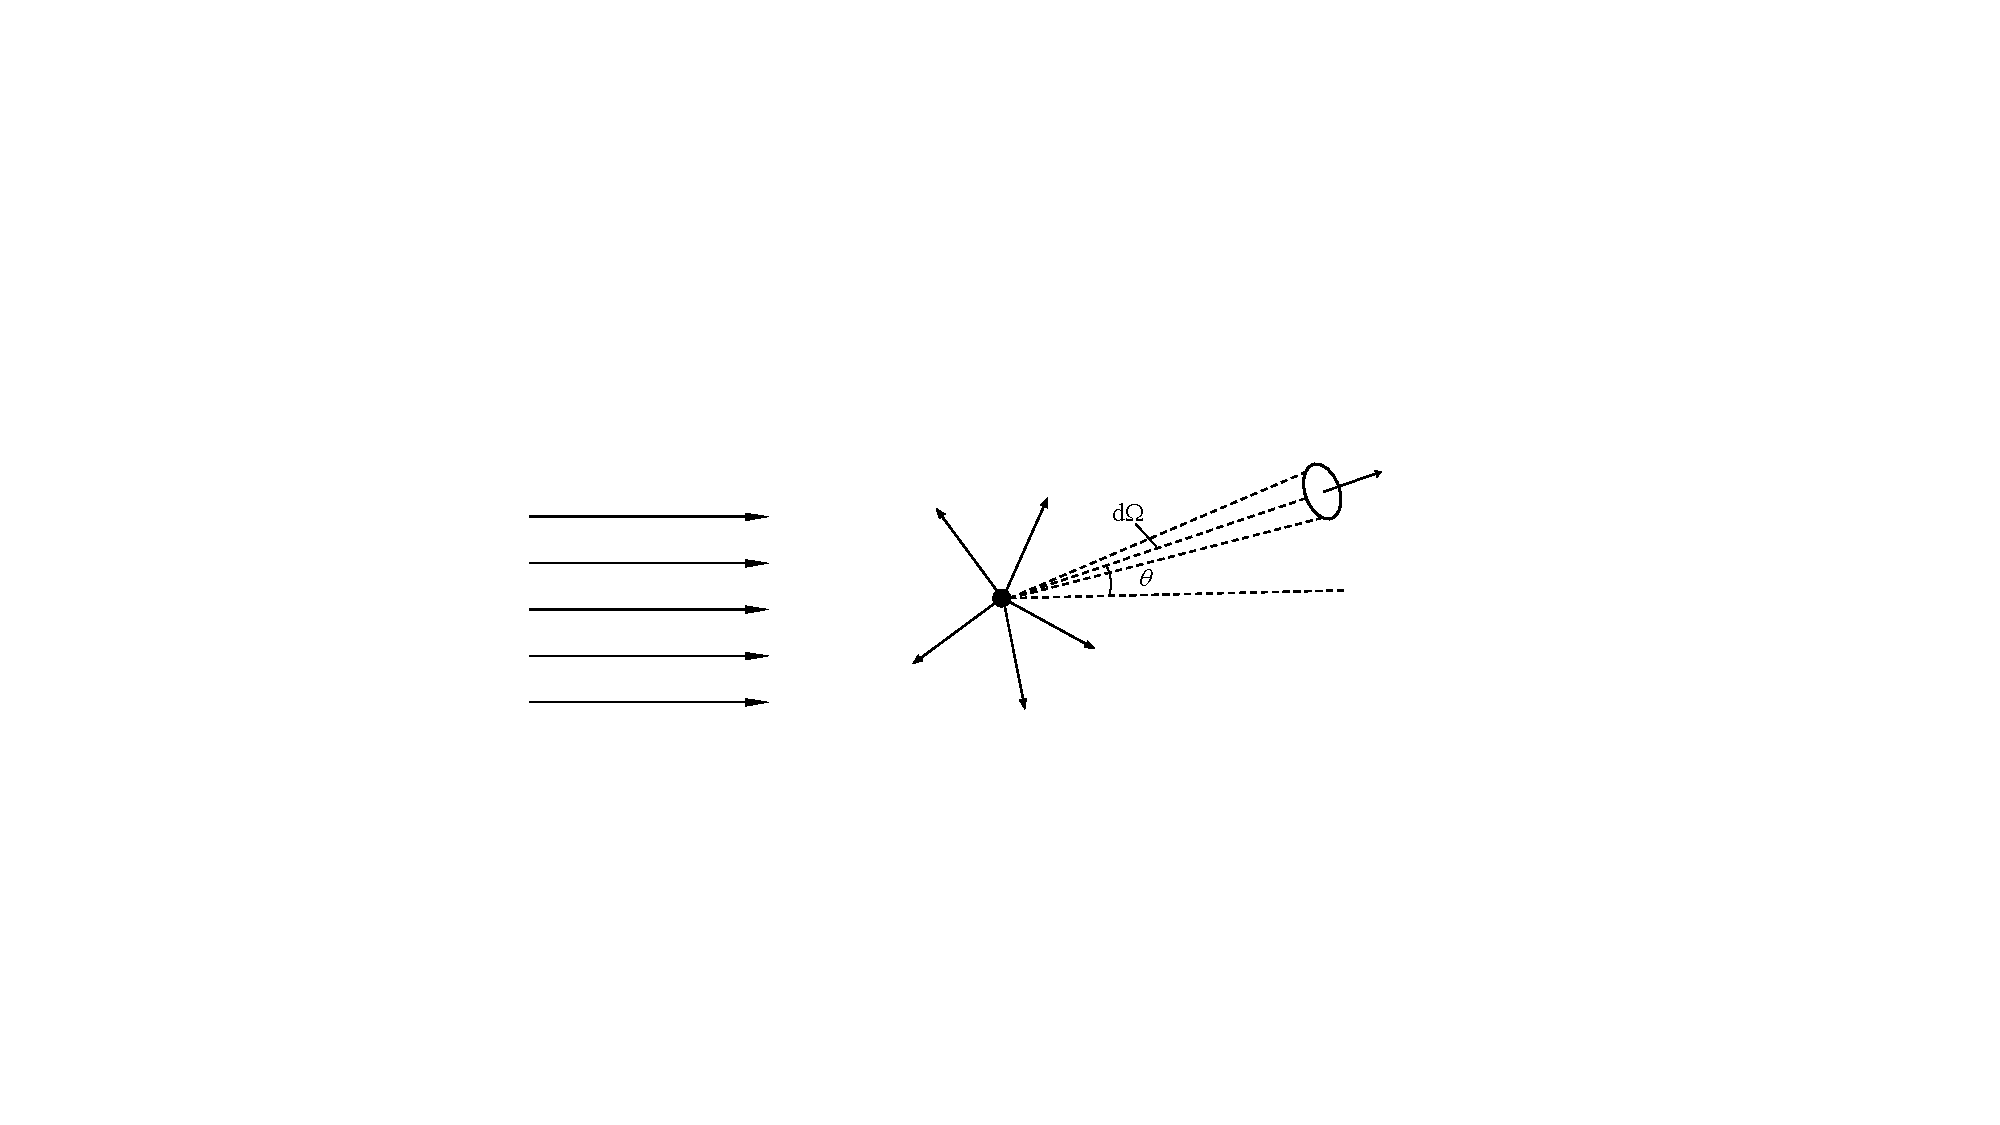
\includegraphics[width=6cm,clip]{QM file/figure/8-1}
	\caption{}\label{fig.8-1}
\end{figure}
粒子运动方向的偏转角称为散射角,即图中$\theta$.考虑一束速度为$v$的入射粒子,入射流量(入射方向单位横截面上,单位时间内通过的粒子数)为$N_{0}$,单位时间内散射的(改变了运动方向的)粒子数为$N$,其中散射到角范围$d\Omega$内的粒子数为$dN$.显然$N$与$dN$均和$N_{0}$成正比,令
\eqshort
\begin{empheq}{align}
	dN &= N_{0}\sigma(\theta,\varphi)d\Omega	\label{eq81.1}	\\
	N  &= \int dN=\sigma_{\text{总}}N_{0}		\label{eq81.2}
\end{empheq}
$\sigma(\theta.\varphi)$与$\sigma_{\text{总}}$的量纲均为面积,$\sigma_{\text{总}}$称为有效总散射截面,意义为,就散射的总效果而言,靶粒子(作用势$V$)相当于挡在入射粒子前进路上的一块横截面$\sigma_{\text{总}}$.$\sigma(\theta,\varphi)$称为有效微分散射截面,它和角元$d\Omega$所处的方向有关,其值取决于作用势$V$的性质.显然
\begin{empheq}{equation}\label{eq81.3}
	\sigma_{\text{总}}=\int\sigma(\theta,\varphi)d\Omega
\end{empheq}
在散射实验中,$N_{0}$和$dN/d\Omega$可以直接测量出来,再利用\eqref{eq81.1}式就得到$\sigma(\theta,\varphi)$的实验值,再由\eqref{eq81.3}式得到$\sigma$的实验值.散射理论的一项主要内容就是建立一套计算$\sigma(\theta,\varphi)$的理论方法,通过理论和实验的比较研究作用势$V$的性质.

{\heiti 2. 散射振幅}

作为散射过程的量子力学描述,入射粒子束可以近似地用平面波描述.以入射方向为$z$轴方向,入射粒子的动量表示成
\begin{empheq}{equation}\label{eq81.4}
	p=\mu v=\hbar k
\end{empheq}
则入射波为
\begin{empheq}{equation}\label{eq81.5}
	\varPsi_{i}=e^{ikz}
\end{empheq}\eqnormal
入射粒子数流量规定成
\begin{empheq}{align}\label{eq81.6}
	N_{0} &=j_{i}=-\frac{i\hbar}{2\mu}\bigg(\varPsi_{i}^{*}\frac{\partial}{\partial r}\varPsi_{i}-\varPsi_{i}\frac{\partial}{\partial r}\varPsi_{i}^{*}\bigg)	\nonumber\\
	&=\frac{\hbar k}{\mu}=v
\end{empheq}
($\varPsi_{i}^{*}\varPsi_{i}=1$,即规定单位体积内入射粒子数为1)
\noindent 散射过程的总波函数$\varPsi$可以表示成入射波$\varPsi_{i}$与散射波$\varPsi_{s}$之和,
\begin{empheq}{equation}\label{eq81.7}
	\varPsi=\varPsi_{i}+\varPsi_{s}=e^{ikz}+\varPsi_{s}
\end{empheq}
对于弹性散射,能量守恒,$\varPsi$满足定态薛定谔方程
\begin{empheq}{equation}\label{eq81.8}
	-\frac{\hbar^{2}}{2\mu}\nabla^{2}\varPsi+V(\boldsymbol{r})\varPsi=E\varPsi
\end{empheq}
其中$E=\frac{p^{2}}{2\mu}=\frac{\hbar^{2}k^{2}}{2\mu}$.通常,散射作用势$V$仅在小范围内起作用,$r\rightarrow\infty$处$V$迅速趋于0,这时\eqref{eq81.8}式变成自由粒子方程:
\begin{empheq}{equation}\label{eq81.9}
	\nabla^{2}\varPsi+k^{2}\varPsi\approx0\quad (r\rightarrow\infty)
\end{empheq}
入射波$\varPsi_{i}$是\eqref{eq81.9}式的一个严格解.$r\rightarrow\infty$处散射波$\varPsi_{s}$应该是\eqref{eq81.9}式的近似解,并取由散射中心$(r=0)$向外传播的球面波形式,即
\begin{empheq}{equation}\label{eq81.10}
	\varPsi_{s}\sim f(\theta,\varphi)\frac{e^{ikr}}{r}\quad (r\rightarrow\infty)
\end{empheq}
其中$f(\theta,\varphi)$称为散射振幅,它与方向$(\theta,\varphi)$有关.容易验证,当$r\rightarrow\infty$,如果略去$r^{-2}$以下小量,则不论$f(\theta,\varphi)$取什么函数形式,\eqref{eq81.10}式都能满足\eqref{eq81.9}式.这表明,在远离散射中心处$(r\rightarrow\infty)$,散射粒子又回到自由运动状态,\eqref{eq81.10}式正是自由粒子外向球面波波函数的一般近似表达式.(略去$r^{-2}$以下小量)一般需要解\eqref{eq81.8}式才能求得散射振幅$f(\theta,\varphi)$.

实验测量是在远离散射中心处进行的,相当于$r\rightarrow\infty$.如果略去$r^{-3}$以下小量,散射粒子数流量为
\begin{empheq}{align*}
	j_{s} &=-\frac{i\hbar}{2\mu}\bigg(\varPsi_{s}^{*}\frac{\partial}{\partial r}\varPsi_{s}-\varPsi_{s}\frac{\partial}{\partial r}\varPsi_{s}^{*}\bigg)	\\
	&=v|f(\theta,\varphi)|^{2}\bigg/ r^{2}
\end{empheq}
在角元$d\Omega$的横截面$r^{2}d\Omega$上单位时间内通过的散射粒子数为
\begin{empheq}{equation}\label{eq81.11}
	dN=j_{s}r^{2}d\Omega=v|f(\theta,\varphi)|^{2}d\Omega
\end{empheq}
与\eqref{eq81.1}式、\eqref{eq81.6}式比较,即得
\begin{empheq}{equation}\label{eq81.12}
	\sigma(\theta,\varphi)=|f(\theta,\varphi)|^{2}
\end{empheq}
散射理论的一项基本内容就是设法求出散射振幅$f(\theta,\varphi)$,从而算出微分散射截面$\sigma(\theta,\varphi)$.

{\heiti 3. 散射过程的经典力学描述}

在经典力学中,每个粒子均有一条运动轨道.以中心力场$V(r)$造成的散射为例,粒子的运动轨迹是一条平面曲线($\varphi$角不变),入射方向与出射方向的夹角就是散射角$\sigma$,如图\ref{fig.8-2}所示.散射角$\sigma$由碰撞参数(瞄准距离)$\rho$决定.经由横截面元$|\rho d\varphi d\rho|$的入射粒子,散射后进入$\theta$方向附近$d\Omega$角范围内,亦即
\begin{empheq}{equation}\label{eq81.13}
	dN=N_{0}|\rho d\rho d\varphi|=N_{0}\sigma(\theta)|d\Omega|
\end{empheq}

\begin{figure}[!h]
	\centering
	\small
	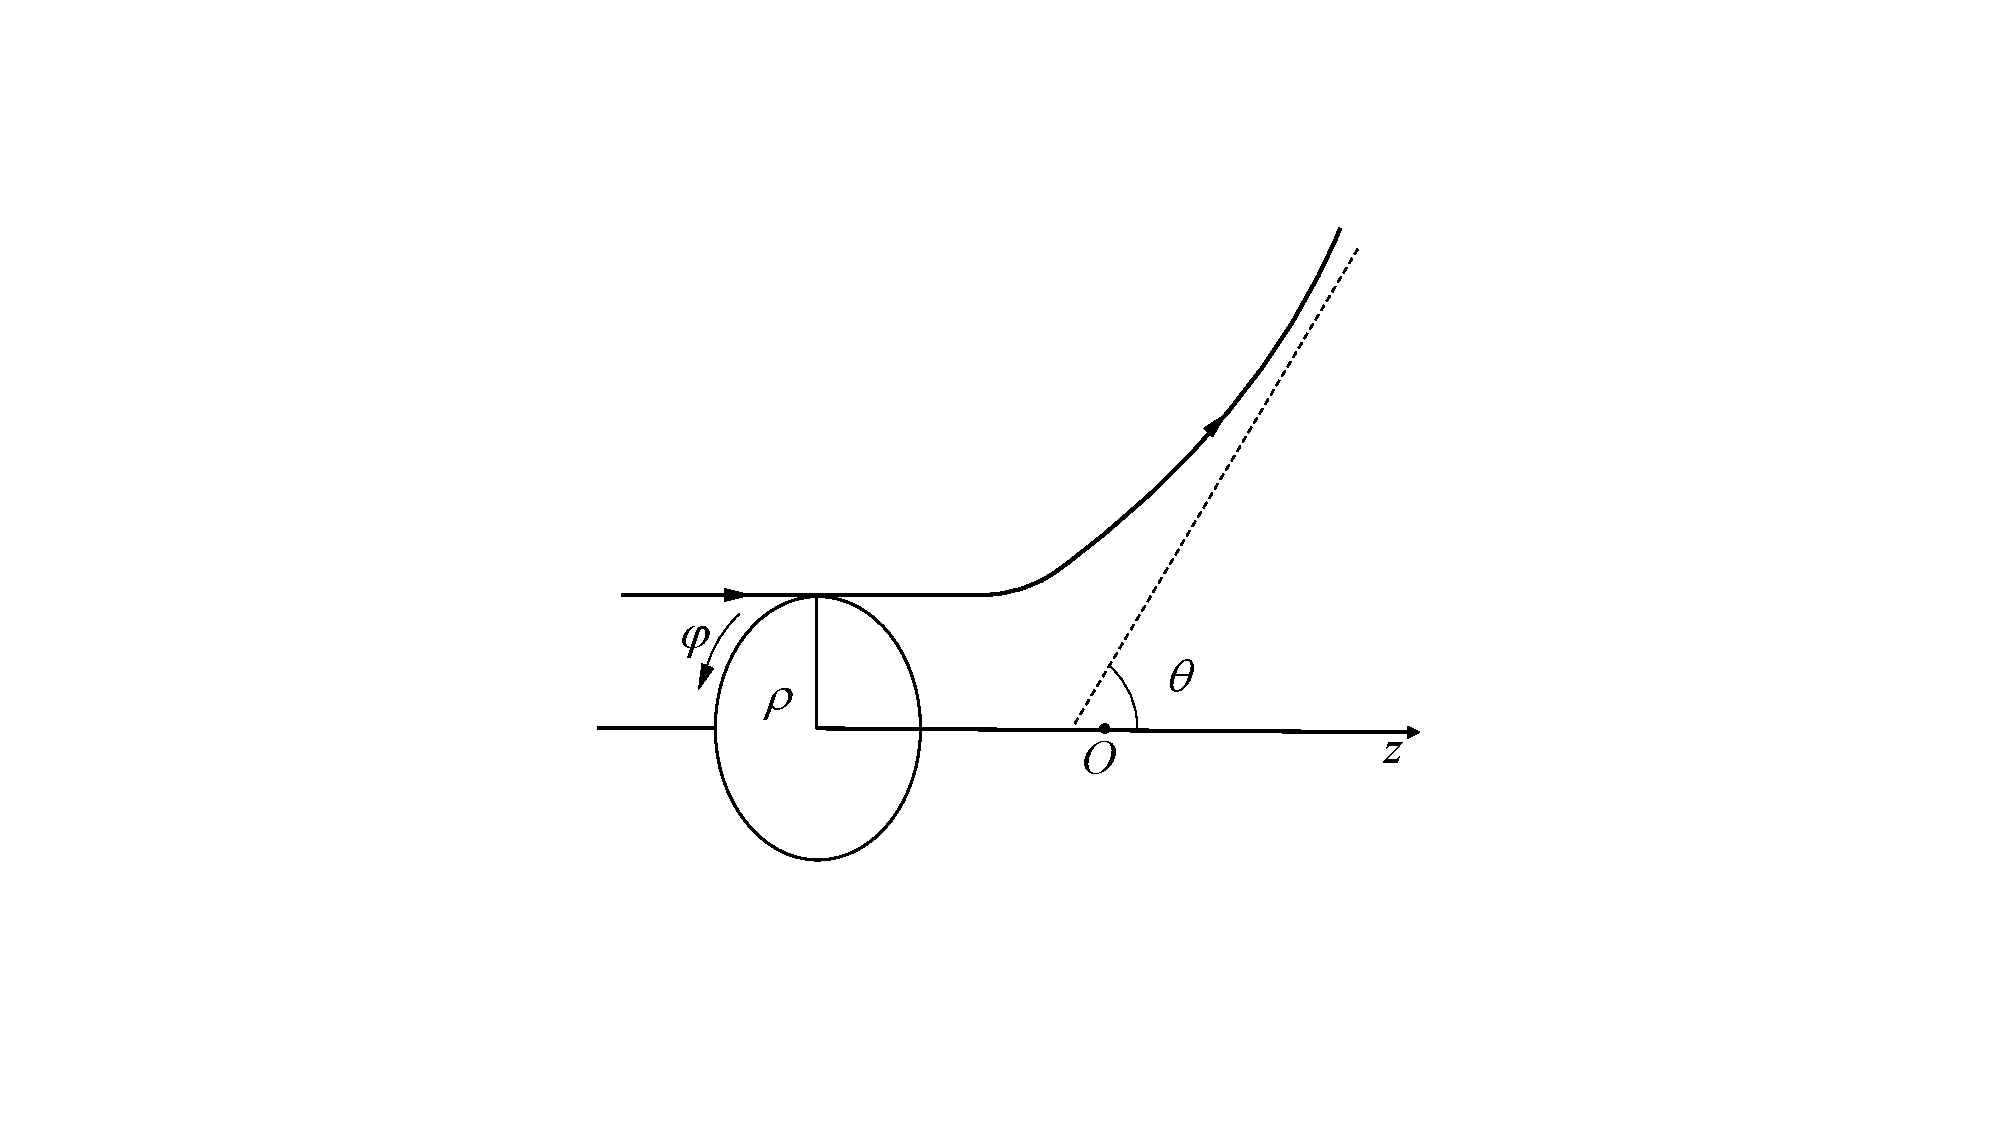
\includegraphics[width=4cm,clip]{QM file/figure/8-2}
	\caption{}\label{fig.8-2}
\end{figure}
其中$d\Omega=\sin\theta d\theta d\varphi$.由上式可得微分散射截面$\sigma(\theta)$的经典力学公式
\begin{empheq}{equation}\label{eq81.14}
	\sigma(\theta)=\left|\frac{\rho d\rho}{\sin\theta d\theta}\right|		%\bigg|\frac{\rho d\rho}{\sin\theta d\theta}\bigg|
\end{empheq}
经典散射理论的核心问题就是求碰撞参数$\rho$与散射角$\theta$的函数关系,从而得到$\sigma(\theta)$的公式.
\pskip

\example 速度为$v$的粒子束被半径为$a$的刚体球散射,求经典弹性散射截面.

\solution 总散射截面显然等于刚球的几何截面$\pi a^{2}$.下面求微分散射截面$\sigma(\theta)$.粒子与刚球碰撞发生弹性散射,入射角等于反射角,由图\ref{fig.8-3}容易看出下列关系:

\begin{figure}[!h]
	\centering
	\small
	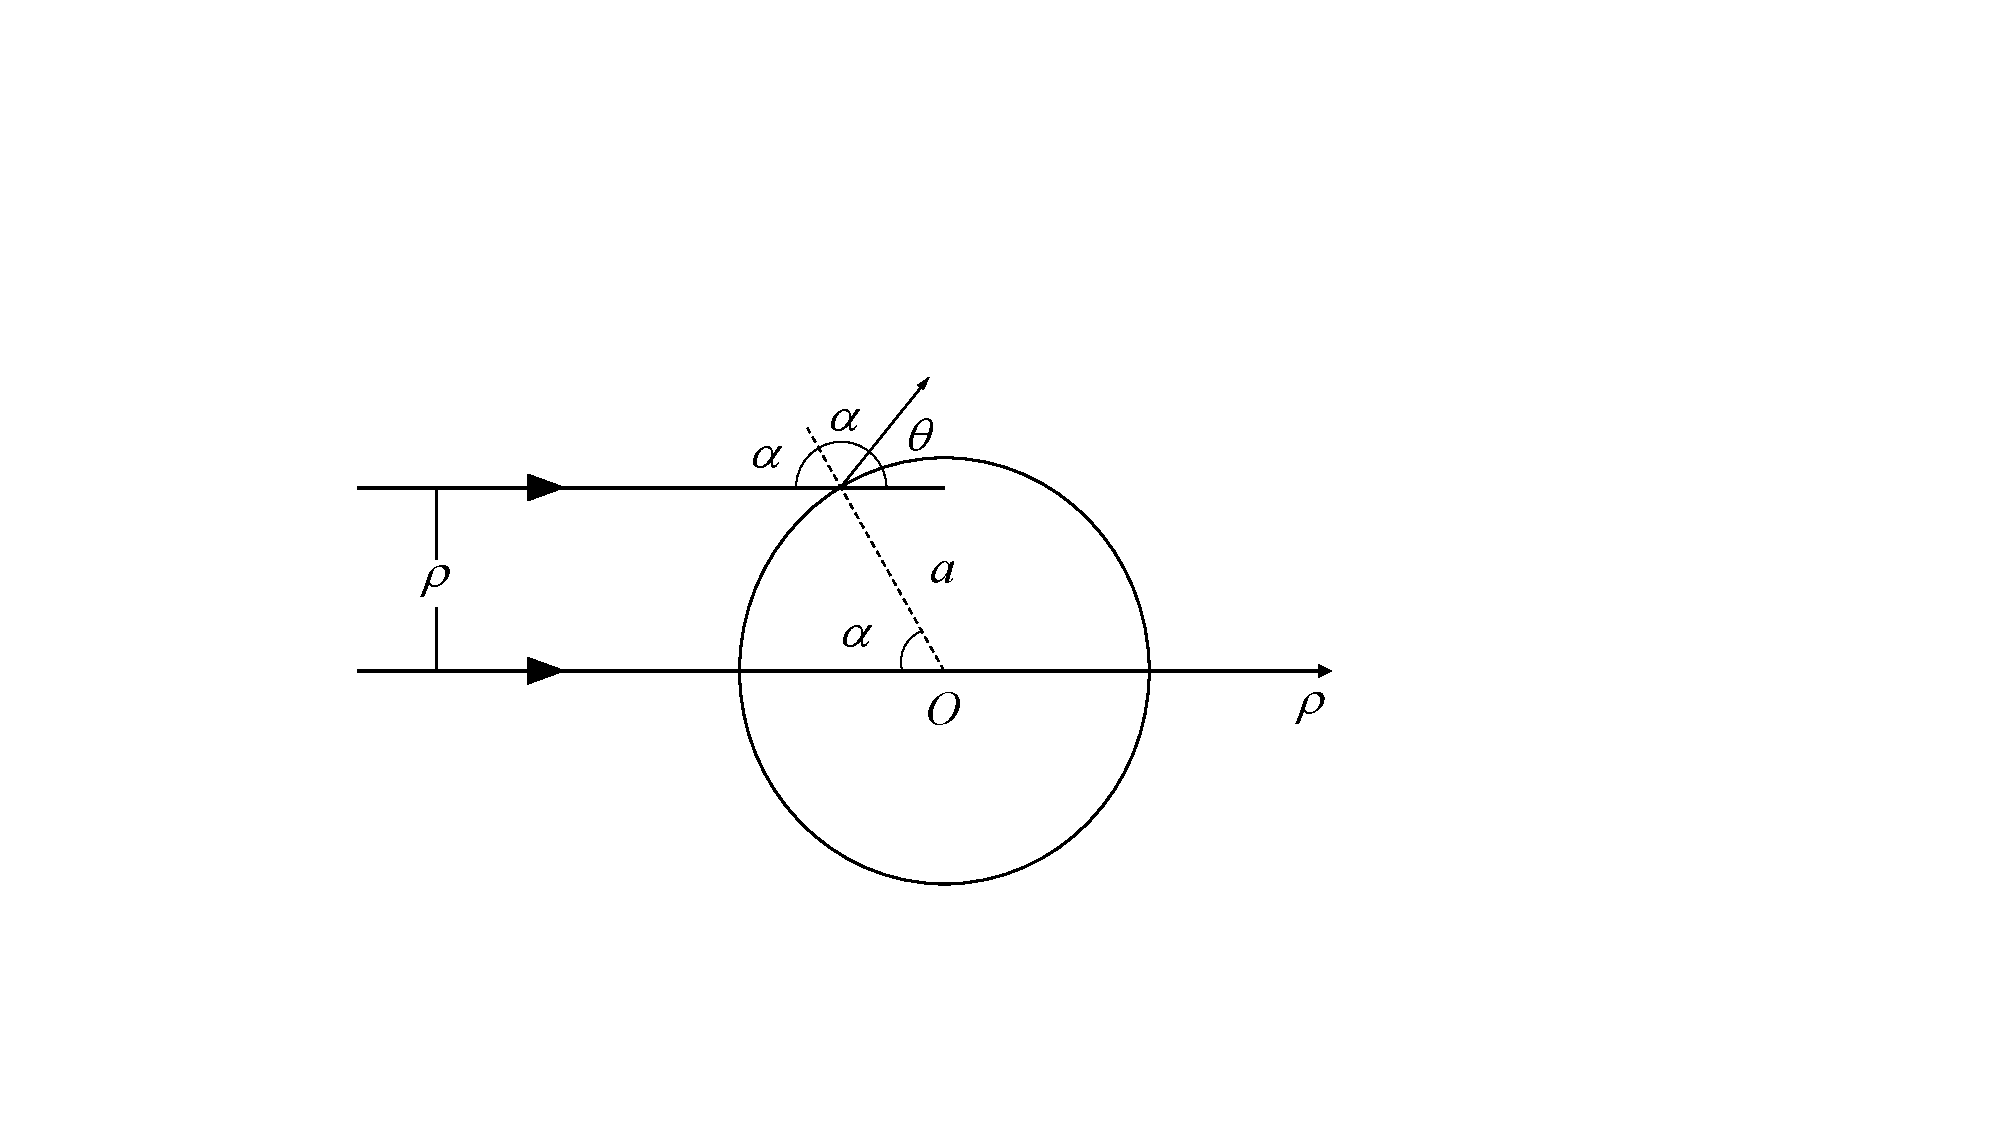
\includegraphics[width=5cm,clip]{QM file/figure/8-3}
	\caption{}\label{fig.8-3}
\end{figure}

\eqshort
\begin{empheq}{align*}
	&\theta+2\alpha=\pi	\\
	\rho= &a\sin\alpha=a \cos\frac{\theta}{2}
\end{empheq}\eqnormal
因此
\begin{empheq}{align*}
	\rho d\rho &=-\frac{a^{2}}{2}\cos\frac{\theta}{2}\sin\frac{\theta}{2}d\theta	\\
	&=-\frac{a^{2}}{4}\sin\theta d\theta
\end{empheq}
代入\eqref{eq81.14}式,即得
\eqshort
\begin{empheq}{equation}\label{eq81.15}
	\sigma(\theta)=a^{2}/4
\end{empheq}\eqnormal
$\sigma(\theta)$与$\theta$无关,这表示散射是各方向均匀的.显然
\begin{empheq}{align}\label{eq81.16}
	\sigma_{\text{总}} &=\int\sigma(\theta)d\Omega	\nonumber\\
		&= 4\pi\sigma(\theta)=\pi a^{2}
\end{empheq}



% 分波法
\section[分波法]{分波法} \label{sec:08.02} % 
% \makebox[5em][s]{} % 短题目拉间距

分波法是研究中心力场散射的普遍方法,其中心思想是将波函数展开成$(\boldsymbol{L}^{2},L_{z})$共同本征函数的线性叠加,然后逐项进行计算.

设散射作用势$V=V(r)$,与方向无关.这时粒子的轨道角动量$\boldsymbol{L}$是守恒量.取守恒量完全集为$(H,\boldsymbol{L}^{2},L_{z})$.入射波波函数的球坐标表示式为
\begin{empheq}{equation*}
	\varPsi_{i}=e^{ikz}=e^{ikr\cos\theta}
\end{empheq}
显然这是$L_{z}$的本征函数(本征值$m\hbar=0$),但不是$\boldsymbol{L}^{2}$的本征函数.如将$\varPsi_{k}$表示成$(\boldsymbol{L}^{2},L_{z})$共同本征函数$Y_{lm}$的线性叠加,可得[见\eqref{eq52.26}式]
\begin{empheq}{equation}\label{eq82.1}
	\varPsi_{i}=e^{ikr\cos\theta}=\sum_{l=0}^{\infty}(2l+1)e^{il\pi/2}j_{l}(kr)P_{l}(\cos\theta)
\end{empheq}
其中$P_{l}$是勒让德多项式,它与$Y_{l0}$只相差一个常系数,
\begin{empheq}{equation}\label{eq82.2}
	Y_{l0}=\sqrt{\frac{2l+1}{4\pi}}P_{l}(\cos\theta)
\end{empheq}
$j_{l}$是球贝塞耳函数,它是自由粒子球面波的径向波函数.我们将\eqref{eq82.1}式写成
\begin{empheq}{equation*}\label{eq82.1'}
	\varPsi=\frac{1}{kr}\sum_{l=0}^{\infty}u_{l}^{(0)}(r)Y_{l0}(\theta)
	\tag{$8.2.1^{\prime}$}
\end{empheq}
其中
\begin{empheq}{align}
	u_{l}^{(0)}&(r) =A_{l}^{(0)}krj_{l}(kr)			\label{eq82.3}\\
	A_{l}^{(0)}&=\sqrt{4\pi(2l+1)}e^{il\pi/2}		\label{eq82.4}
\end{empheq}
$u_{l}^{(0)}$满足自由粒子径向方程[见\eqref{eq52.4}式]
\begin{empheq}{equation}\label{eq82.5}
	\frac{d^{2}}{dr^{2}}u_{l}^{(0)}+\bigg[k^{2}-\frac{l(l+1)}{r^{2}}\bigg]u_{l}^{(0)}=0
\end{empheq}
根据$\S$\ref{sec:05.02}的讨论,$r\rightarrow\infty$处有下列渐近行为:
\begin{empheq}{align}
	j_{l}(kr)&\approx\frac{1}{kr}\sin\bigg(kr-\frac{l\pi}{2}\bigg)		\label{eq82.6}	\\
	u_{l}^{(0)}(r)&\approx A_{l}^{(0)}\sin\bigg(kr-\frac{l\pi}{2}\bigg)		\nonumber	\tag{$8.2.6^{\prime}$}	\label{eq82.6'}
\end{empheq}
在入射波也中,第$l$项分波($Y_{l0}$项)的相对比重显然与$|A_{l}^{(0)}|^{2}$成比例,亦即与$(2l+1)$成比例.在经典散射理论中,入射粒子束(参看图\ref{fig.8-2})的$L_{z}$仍为0,而$|\boldsymbol{L}|\propto\rho$,角动量值在$(L,L+\Delta L)$间的入射粒子数与$2\pi\rho\Delta\rho$成比例,亦即与$L\Delta L$成比例,如取$\Delta L=\hbar$,以及
\begin{empheq}{equation*}
	L\sim \sqrt{l(l+1)}\hbar\sim \bigg(l+\frac{1}{2}\bigg)\quad (l\gg 1)
\end{empheq}
则角动量取某个$L$值的入射粒子数与$L$成比例,并大致与$\bigg(l+\frac{1}{2}\bigg)$成比例,这个结论和量子力学结论一致.

经过散射后的总波函数$\varPsi$满足定态薛定谔方程
\begin{empheq}{equation}\label{eq82.7}
	-\frac{\hbar^{2}}{2\mu}\nabla^{2}\varPsi+V(r)\varPsi=\frac{\hbar^{2}k^{2}}{2\mu}\varPsi
\end{empheq}
由于是中心力场,$\boldsymbol{L}^{2},L_{z}$守恒,$l,m$是好量子数,其取值及概率分布不受$V(r)$的影响,如将$\varPsi$表示成$(H,\boldsymbol{L}^{2},L_{z})$共同本征函数的线性叠加,将是
\begin{empheq}{equation}\label{eq82.8}
	\varPsi(r,\theta)=\frac{1}{kr}\sum_{l=0}^{\infty}u_{l}(r)Y_{l0}(\theta)
\end{empheq}
$\varPsi$与$\varPsi_{i}$的差别在于$u_{l}^{(0)}$变成了$u_{l}$,后者满足径向方程
\begin{empheq}{equation}\label{eq82.9}
	\frac{d^{2}}{dr^{2}}u_{l}+\left[k^{2}-\frac{l(l+1)}{r^{2}}-\frac{2\mu}{\hbar^{2}}V(r)\right]u_{l}=0
\end{empheq}
给定$V(r)$后,由上式即可解出$u_{l}$.下面讨论$r\rightarrow\infty$处$u_{l}$的渐近行为.$r\rightarrow\infty$处$V(r)$一般均迅速趋于0,这时\eqref{eq82.9}式中$V(r)$及离心势($r^{-2}$项)均可略去,成为
\begin{empheq}{equation}\label{eq82.10}
	\frac{d^{2}}{dr^{2}}u_{l}+k^{2}u_{l}\approx 0
\end{empheq}
其渐近解为
\begin{empheq}{equation}\label{eq82.11}
	u_{l}(r)\approx A\sin\left(kr-\frac{l\pi}{2}+\delta_{l}\right)
\end{empheq}
$A_{l}$和$\delta_{l}$是待定常数.将\eqref{eq82.11}式和\eqref{eq82.6'}式比较,可知$u_{l}^{(0)}$与$u_{l}$的渐近性质存在两方面的差别:

(i) 振幅由$A_{l}^{(0)}$变成$A_{l}$;

(ii) $u_{l}$的渐近形式中增添了“相移”$\delta_{l}$.
当然,这都是散射造成的后果.

将\eqref{eq82.6'}式代入\eqref{eq82.1'}式,并利用公式
\begin{empheq}{equation*}
	\sin x=\frac{e^{ix}-e^{-ix}}{2i}
\end{empheq}
可得$r\rightarrow\infty$处$\varPsi_{i}$的渐近形式
\eqlong
\begin{empheq}{equation}\label{eq82.12}
	\varPsi_{i}\approx\frac{1}{2ikr}\sum_{l}A_{l}^{(0)}(e^{ikr}e^{-il\pi/2}-e^{-ikr}e^{il\pi/2})Y_{l0}(\theta)
\end{empheq}
而将\eqref{eq82.11}式代入\eqref{eq82.8}式可得$\varPsi$的渐近形式
\begin{empheq}{equation}\label{eq82.13}
	\varPsi_{i}\approx\frac{1}{2ikr}\sum_{l}A_{l}[e^{ikr}e^{i(\delta_{l}-l\pi/2)}-e^{-ikr}e^{i(l\pi/2-\delta_{l})}]Y_{l0}(\theta)
\end{empheq}\eqnormal
由于
\begin{empheq}{equation}\label{eq82.14}
	\varPsi-\varPsi_{i}=\varPsi_{s}\approx f(\theta)\frac{e^{ikr}}{r}
\end{empheq}
\eqref{eq82.12}式和\eqref{eq82.13}式中$e^{-ikr}$项应该相同,由此可知
\begin{empheq}{equation}\label{eq82.15}
	A_{l}=A_{l}^{(0)}e^{i\delta_{l}}
\end{empheq}
以及
\begin{empheq}{equation*}
	f(\theta)=\frac{1}{2ik}\sum_{l}(A_{l}e^{i\delta_{l}}-A_{l}^{(0)})e^{-il\pi/2}Y_{l0}(\theta)
\end{empheq}
将\eqref{eq82.4}式及\eqref{eq82.15}式代入上式,经过化简,即得散射振幅$f(\theta)$与各分波相移$\delta_{l}$的关系式
\begin{empheq}{align}\label{eq82.16}
	f(\theta) &=\frac{\sqrt{4\pi}}{k}\sum_{l=0}^{\infty}\sqrt{2l+1}\sin\delta_{l}e^{i\delta_{l}}Y_{l0}(\theta)		\nonumber\\
	&=\frac{1}{k}\sum_{l=0}^{\infty}(2l+1)\sin\delta_{l}e^{i\delta_{l}}P_{l}(\cos\theta)	\nonumber\\
	&=\sum_{l=0}^{\infty}f_{l}(\theta)
\end{empheq}
其中$f_{l}(\theta)$为第$l$个分波造成的散射振幅,即
\begin{empheq}{equation}\label{eq82.17}
	\frac{1}{kr}[u_{l}-u_{l}^{(0)}]Y_{l0}(\theta)\approx f_{l}(\theta)\frac{e^{ikr}}{r}
\end{empheq}
在散射过程中,各个分波各自独立地产生相移$\delta_{l}$,并对散射振幅作出独立的贡献.根据\eqref{eq81.12}式,微分散射截面为
\begin{empheq}{equation}\label{eq82.18}
	\sigma(\theta)=f^{*}(\theta)f(\theta)
\end{empheq}
散射振幅及微分散射截面均与$\varphi$角无关,散射结果呈轴对称分布(以$z$轴为对称轴),这是中心力散射的特点.

如用各分波散射振幅来表示,$\sigma(\theta)$可以写成
\begin{empheq}{equation*}\label{eq82.18'}
	\sigma(\theta)=\sum_{l}\sum_{l^{\prime}}f_{l}^{*}(\theta)f_{l}(\theta)
	\tag{$8.2.18^{\prime}$}
\end{empheq}
各个分波散射振幅并不是对$\sigma(\theta)$作出独立的贡献,而是相互间存在干涉效应.总散射截面的构成情况则有所不同,由\eqref{eq81.3}式,
\begin{empheq}{align}\label{eq82.19}
	\sigma_{\text{总}} &=\int\sigma(\theta)d\Omega	\nonumber\\
	&= \sum_{l}\sum_{l^{\prime}}\int f_{l}^{*}(\theta)f_{l^{\prime}}(\theta)d\Omega
\end{empheq}
由于$f_{l}$中含有$Y_{l0}(\theta)$,而球谐函数具有正交性
\begin{empheq}{equation*}
	\int Y_{l0}^{*}(\theta)Y_{l^{\prime}0}(\theta)d\Omega=\delta_{ll^{\prime}}
\end{empheq}
因此\eqref{eq82.19}式中仅$l=l^{\prime}$的项对积分有贡献.容易算出
\begin{empheq}{align}
	\sigma_{\text{总}}=\sum_{l}&\int f_{l}^{*}(\theta)f_{l}(\theta)d\Omega=\sum_{l}\sigma_{l}	\label{eq82.20}\\
	\sigma_{l}=&\int f_{l}^{*}(\theta)f_{l}(\theta)d\Omega	\nonumber\\
	=&\frac{4\pi}{k^{2}}(2l+1)\sin^{2}\delta_{l}		\label{eq82.21}
\end{empheq}
在$\sigma_{\text{总}}$的构成中,干涉效应消失,各个分波各自独立地对$\sigma_{\text{总}}$作出贡献,$\sigma_{l}$称为第$l$分波的散射截面.

当散射角$\theta\rightarrow0$,散射振幅$f$的值有特殊意义.当$\theta\rightarrow0$,\eqref{eq82.16}式中$P_{l}(1)=1$,因此
\begin{empheq}{equation}\label{eq82.22}
	f(0)=\frac{1}{k}\sum_{l}(2l+1)\sin\delta_{l}e^{i\delta_{l}}=\sum_{l}f_{l}(0)
\end{empheq}
容易看出
\begin{empheq}{align}
	\sigma_{l} &=\frac{4\pi}{k}\lm f_{l}(0)		\label{eq82.23}	\\
	\sigma_{\text{总}} &=\frac{4\pi}{k}\lm f(0)		\label{eq82.24}
\end{empheq}
($\lm$表示取虚部)这个结果称为光学定理.

用分波法处理中心力散射,关键是先要求出各级分波相移$\delta_{l}$,然后由\eqref{eq82.16}式和\eqref{eq82.18}式就可得出散射振幅$f(\theta)$和微分散射截面$\sigma(\theta)$.求$\delta_{l}$的基本方法是解径向方程\eqref{eq82.9}式,并辅以各种近似方法.下面介绍一种计算$\delta_{l}$的近似公式.

以$u_{l}^{(0)}$左乘\eqref{eq82.9}式,$u_{l}$左乘\eqref{eq82.5}式,相减即得
\begin{empheq}{equation*}
	\frac{d}{dr}\left[u_{l}^{(0)}\frac{du_{l}}{dr}-u_{l}\frac{du_{l}^{(0)}}{dr}\right]=\frac{2\mu}{\hbar^{2}}V(r)u_{l}u_{l}^{(0)}
\end{empheq}
对$r$积分,得到
\eqlong
\begin{empheq}{equation*}
	\frac{2\mu}{\hbar^{2}}\int_{0}^{\infty}V(r)u_{l}u_{l}U(0)dr=\left[u_{l}^{(0)}\frac{du_{l}}{dr}-u_{l}\frac{du_{l}^{(0)}}{dr}\right]\big|_{r=0}^{r\rightarrow\infty}
\end{empheq}\eqnormal
当$r=0$,上式右端为0;当$r\rightarrow\infty$,由\eqref{eq82.6'}及\eqref{eq82.11}式,上式右端为$(-kA_{l}A_{l}^{(0)}\sin\delta_{l})$,因此
\begin{empheq}{equation}\label{eq82.25}
	\sin\delta_{l}=-\frac{2\mu}{\hbar^{2}kA_{l}A_{l}U(0)}\int_{0}^{\infty}V(r)u_{l}u_{l}U(0)dr
\end{empheq}
至此是严格的.如某个分波散射较弱,$|\delta_{l}|\ll 1$,(条件见下面的叙述)则上式中可以用$u_{l}^{(0)}$代替$u_{l}$,$A_{l}^{(0)}$代替$A_{l}$,从而得到
\begin{empheq}{equation}\label{eq82.26}
	\sin\delta_{l}\approx\delta_{l}\approx-\frac{2\mu k}{\hbar^{2}}\int_{0}^{\infty}V(r)[j_{l}(kr)]^{2}r^{2}dr
\end{empheq}
由上式容易看出,如果$V>O$(排斥力),则$\delta_{l}<0$;如果$V<O$(吸引力),则$\delta_{l}>0$.在许多场合,散射作用势$V$仅在一定距离内($r\leqslant a$,$a$称为作用球半径.)才有显著值,这时\eqref{eq82.26}式的积分上限可以换成$a$.这种情况下,按照经典散射模型,能够产生显著散射的最大碰撞参数为$\rho_{max}\approx a$,最大角动量为$L_{max}\approx\hbar ka$.常称$ka\gg 1$的情况为高能散射,这时需要考虑的分波数目较多$(l_{max}\gg 1)$,用分波法处理较为麻烦,$ka\ll 1$的情况称为低能散射,这时经典$L_{max}\ll\hbar$,用分波法处理只需考
虑$l=0$这一分波(所谓s波),即可获得散射的主要信息.对于低能s波散射,
\begin{empheq}{align}
	f(\theta) &\approx f_{0}=\frac{1}{k}\sin\delta_{0}e^{i\delta_{0}}		\label{eq82.27}	\\
	\sigma(\theta) &\approx |f_{0}|^{2}=\frac{1}{k^{2}}\sin^{2}\delta_{0}		\label{eq82.28}
\end{empheq}
散射的角分布是各向同性的.
\pskip

\example 刚体球散射的分波法处理.

刚体球(半径$a$)的量子力学含义是
\begin{empheq}{equation*}
	{V(r)=}
	\begin{dcases}
		0,\qquad  r>a	\\
		\infty, \quad r\leqslant a
	\end{dcases}
\end{empheq}
在球内区域$(r\leqslant a)$波函数$\varPsi=0$.入射波仍由\eqref{eq82.1}式表示,散射后总波函数仍由\eqref{eq82.8}式表示在球外区域$(r>0)V=0$,因此径向方程\eqref{eq82.9}式形式上和\eqref{eq82.5}式相同,亦即和\eqref{eq52.4}式相同.\eqref{eq82.9}式有两个独立解,一个就是$kr_{l}(kr)$;另一个解在$\S$\ref{sec:05.02}中曾经提到,但随即以$r\rightarrow0$处边界条件为由予以舍弃,这个解通常记为$krn_{l}(kr)$,$n_{l}$称为球诺依曼函数,其定义为
\begin{empheq}{align}\label{eq82.29}
	n_{l}(\rho) &=(-1)^{(l+1)}\sqrt{\frac{\pi}{2\rho}}J_{-l-\frac{1}{2}}(\rho)	\nonumber\\
	&= (-1)^{l+1}\rho^{l}\left(\frac{1}{\rho}\frac{d}{d\rho}\right)^{l}\frac{\cos\rho}{\rho}
\end{empheq}
亦即在$j_{l}(\rho)$的定义[\eqref{eq52.16}式]中将$\sin\rho$换成$(-\cos\rho)$,就成为$n_{l}(\rho)$.$\rho\rightarrow\infty$处$n_{l}$的渐近形式为
\begin{empheq}{equation}\label{eq82.30}
	n_{l}(\rho)\approx-\frac{1}{\rho}\cos\left(\rho-\frac{l\pi}{2}\right)
\end{empheq}
对于本题,在球外区域,第$l$分波的径向波函数应该取
\begin{empheq}{equation}\label{eq82.31}
	R_{l}(r)=\frac{u_{l}(r)}{kr}=c_{l}j_{l}(kr)+b_{l}n_{l}(kr)
\end{empheq}
$R_{l}$还必须满足边界条件$R_{l}(r=a)=0$,由此易得
\eqshort
\begin{empheq}{equation}\label{eq82.32}
	b_{l}/c_{l}=-\frac{j_{l}(ka)}{n_{l}(ka)}
\end{empheq}\eqnormal
当$r\rightarrow\infty$,$u_{l}$的渐近形式为
\begin{empheq}{equation*}
	u_{l}(r) \approx c_{l}\sin\bigg(kr-\frac{l\pi}{2}\bigg)-b_{l}\cos\bigg(kr-\frac{l\pi}{2}\bigg)
\end{empheq}
而由\eqref{eq82.11}式,
\eqlong
\begin{empheq}{align*}
	u_{l}(r) &\approx A_{l}\sin\bigg(kr-\frac{l\pi}{2}+\delta_{l}\bigg)	\\
	&=A_{l}\cos\delta_{l}\sin\bigg(kr-\frac{l\pi}{2}\bigg)+A_{l}\sin\delta_{l}\cos\bigg(kr-\frac{l\pi}{2}\bigg)
\end{empheq}\eqnormal
比较即得
\begin{empheq}{align}
	c_{l}&= A_{l}\cos\delta_{l},\quad b_{l}=-A_{l}\sin\delta_{l}		\label{eq82.33}	\\
	&\frac{b_{l}}{c_{l}}=-\frac{\sin\delta_{l}}{\cos\delta_{l}}=-\tan\delta_{l} 	\nonumber	\tag{$8.2.33^{\prime}$}\label{eq82.33'}
\end{empheq}
比较\eqref{eq82.32}式及\eqref{eq82.33'}式,得出
\begin{empheq}{equation}\label{eq82.34}
	\tan\delta_{l}=\frac{j_{l}(ka)}{n_{l}(ka)}=(-1)^{l+1}\frac{J_{l+\frac{1}{2}}(ka)}{J_{-l-\frac{1}{2}}(ka)}
\end{empheq}
给定$ka$后,$j_{l}(ka)$及$n_{l(ka)}$的值可由贝塞耳函数表查出,代入上式就可算出$\delta_{l}$,再代入\eqref{eq82.16}式和\eqref{eq82.18}式就得到$f(\theta$和$\sigma(\theta)$.

以上是严格的.下面讨论低能散射和高能散射两种极端情况.对于低能散射,$ka\ll 1$,这时
\begin{empheq}{align}
	j_{l}(ka) &\approx \frac{(ka)^{l}}{(2l+1)!!}			\label{eq82.35}\\
	n_{l}(ka) &\approx -\frac{(2l-1)!!}{(ka)^{l+1}}			\nonumber\\
	\tan\delta_{l} &\approx-\frac{(ka)^{2l+1}}{(2l+1)!!(2l-1)!!}			\label{eq82.36}
\end{empheq}
注意$|\tan\delta_{l}|\ll 1$,所以
\begin{empheq}{equation*}
	\delta_{l}\approx\sin\delta_{l}\approx\tan\delta_{l}\propto(ka)^{2l+1}
\end{empheq}
例如
\eqlong
\begin{empheq}{equation*}
	\delta_{0}=-ka,\quad \delta_{l}\approx -\frac{(ka)^{3}}{3},\quad \delta_{2}\approx-\frac{(ka)^{5}}{45} -\frac{(ka)^{5}}{45}
\end{empheq}\eqnormal
($\delta_{0}$是严格的)随着$l$的增加, $\delta_{l}$减小得很快,所以可以略去一切$l\neq0$的分波散射[$\sigma_{l}\propto\delta_{l}^{2}\propto(ka)^{4l+2}$],只计算s波$(l=0)$散射,结果是
\begin{empheq}{align}\label{eq82.37}
	&\delta_{0}=-ka,\quad f(\theta)\approx f_{0} \approx -ae^{ika}	\nonumber\\
	&\sigma(\theta) \approx a^{2},\quad \sigma_{\text{总}} \approx \sigma_{0} 4\pi a^{2}
\end{empheq}
和经典散射类似,散射角分布是各向同性的.但总散射截面等于球的表面积,为经典散射截面的4倍.

高能散射,$ka\ll 1$.按照经典力学,能够造成散射的最大角动量为$L_{max}=\hbar ka$,即$l_{max}\approx ka$.量子力学结论虽不完全相同,但有显著散射效果的分波其$l$值的量级仍不超过$ka$.[证明较复杂,从略.当$l\gg ka$,\eqref{eq82.35}式即可成立,则$\delta_{l}$仍由\eqref{eq82.36}式表示,这时容易证明$|\delta_{l}|\ll 1$,相应的分波散射截面可以忽略不计.]而当$ka>l$,渐近表示式\eqref{eq82.6}及\eqref{eq82.30}式即可成立,则由\eqref{eq82.34}式可得
\begin{empheq}{equation*}
	\tan\delta_{l} \approx -\frac{\sin\bigg(ka-\frac{l\pi}{2}\bigg)}{\cos\bigg(ka-\frac{l\pi}{2}\bigg)}=-\tan\bigg(ka-\frac{l\pi}{2}\bigg)
\end{empheq}
所以
\eqshort
\begin{empheq}{equation}\label{eq82.38}
	\delta_{l}\approx -\bigg(ka-\frac{l\pi}{2}\bigg)
\end{empheq}
由于$\delta_{l+1}\approx \delta_{l}+\frac{\pi}{2}$,所以
\begin{empheq}{equation*}
	\sin^{2}\delta_{l}+\sin^{2}\delta_{l+1}\approx 1
\end{empheq}\eqnormal
计算$\sigma_{\text{总}}$时,不妨取每一项$\sin^{2}\delta_{l}$的有效值为$\frac{1}{2}$,从而得到
\begin{empheq}{align}\label{eq82.39}
	\sigma_{\text{总}}&\approx \frac{4\pi}{k^{2}}\sum_{l=0}^{ka}\bigg(l+\frac{1}{2}\bigg)	\nonumber\\
	&\approx \frac{4\pi}{k^{2}}\cdot\frac{1}{2}(ka+1)^{2}\approx 2\pi a^{2}
\end{empheq}
其中一半来自经典散射,一半来自衍射.至于$\sigma(\theta)$,由于主要贡献来自于$l\gg 1$的分波,角分布近似于各方向均匀分布.[原因是$P_{l}(\cos\theta)$在$\pm1$间振荡$l$次.]




% 低能散射
\starthis\section[低能散射]{低能散射$^{*}$} \label{sec:08.03} % 
% \makebox[5em][s]{} % 短题目拉间距
% \starthis 章节加星

继续上节的讨论,设散射作用势$V(r)$是短程的,在作用球(半径$a$)以外$V\approx0$.令$E=\frac{\hbar^{2}k^{2}}{2\mu}$,并考虑低能散射,$ka\ll 1$.这时第$l$级分波相移$\delta_{l}$大致与$(ka)^{2l+1}$成比例.[参看\eqref{eq82.26}式和\eqref{eq82.35}式,以及刚球散射.]可以只考虑s波$(l=0)$散射,而略去其他分波$(l\geqslant1)$的贡献.s波径向方程为
\begin{empheq}{equation}\label{eq83.1}
	\frac{d^{2}}{dr^{2}}u_{0}+\bigg[k^{2}-\frac{2\mu}{\hbar^{2}}V(r)\bigg]u_{0}=0
\end{empheq}
取低能极限$E\rightarrow0(k\rightarrow0)$,并研究$r>a$处(作用球外)$u_{0}$的表现形式.这时$V\approx0$,\eqref{eq83.1}式成为
\eqshort
\begin{empheq}{equation}\label{eq83.2}
	\frac{d^{2}}{dr^{2}}u_{0}=0
\end{empheq}
解为
\begin{empheq}{equation}\label{eq83.3}
	u_{0}(r)=c\bigg(1-\frac{r}{a_{0}}\bigg)
\end{empheq}\eqnormal
$c$及$a_{0}$为常数,$a_{0}$称为“散射长度”,其意义稍后再加以说明.

根据\eqref{eq82.11}式,在作用球外应该有渐近形式
\begin{empheq}{align*}
	u_{0}(r) &\approx A_{0}\sin(kr+\delta_{0})	\\
	&=A_{0}\sin\delta_{0}(\cos kr+\cot\delta_{0}\cdot\sin kr)
\end{empheq}
在低能极限下,$k\rightarrow=,\cos kr\rightarrow1,\sin kr\rightarrow kr$,上式成为
\begin{empheq}{equation*}
	u_{0}(r) \approx A_{0}\sin\delta_{0}(1+kr\cot\delta_{0})
\end{empheq}
与\eqref{eq83.3}式比较,可知
\begin{empheq}{equation}\label{eq83.4}
	\boxed{k\cot\delta_{0}=-\frac{1}{a_{0}}\quad(k\rightarrow0)}
\end{empheq}
散射振幅的低能极限为
\begin{empheq}{align}\label{eq83.5}
	f(\theta) &\approx f_{0}=\frac{1}{k}\sin\delta_{0}e^{i\delta_{0}}	\nonumber\\
	&=\frac{1}{k\cot\delta_{0}-ik}=-\frac{a_{0}}{1+ika_{0}}
\end{empheq}
如散射长度$a_{0}$取有限值,则当$k\rightarrow0,k|a_{0}|\ll1$,\eqref{eq83.5}式即
\begin{empheq}{equation}\label{eq83.6}
	f(\theta) \approx-a_{0}\quad (k\rightarrow0)
\end{empheq}
这时\eqref{eq83.4}式给出
\begin{empheq}{equation}\label{eq83.7}
	-ka_{0}=\tan\delta_{0}\approx\sin\delta_{0}\approx\delta_{0}
\end{empheq}
散射截面为
\begin{empheq}{align}\label{eq83.8}
	\sigma(\theta)&=|f(\theta)|^{2}=a_{0}^{2}	\nonumber\\
	\sigma_{\text{总}}&=4\pi a_{0}^{2}
\end{empheq}
这种情况下势场$V(r)$的散射效果相当于半径为$a_{0}$的刚球.注意$\delta_{0}$与$k$成正比,$f(\theta),\sigma(\theta)$均与$k$无关,即与能量$E$无关.

如$a_{0}\rightarrow\pm\infty$,则\eqref{eq83.4}式给出
\begin{empheq}{equation}\label{eq83.9}
	k\cot\delta_{0}=0,\quad \delta_{0}=\frac{\pi}{2},\quad\text{或}\quad -\frac{\pi}{2}
\end{empheq}
而\eqref{eq83.5}式给出
\eqshort
\begin{empheq}{equation}\label{eq83.10}
	f(\theta)=\frac{i}{k}
\end{empheq}\eqnormal
因此
\begin{empheq}{equation}\label{eq83.11}
	\sigma_{\text{总}}=4\pi\sigma(\theta)=\frac{4\pi}{k^{2}}=\frac{2\pi\hbar^{2}}{\mu E}
\end{empheq}
散射截面与$E$成反比.当$E\rightarrow0,\sigma_{\text{总}}\rightarrow\infty$,称为“共振散射”.

\begin{figure}[!h]
	\centering
	\small
	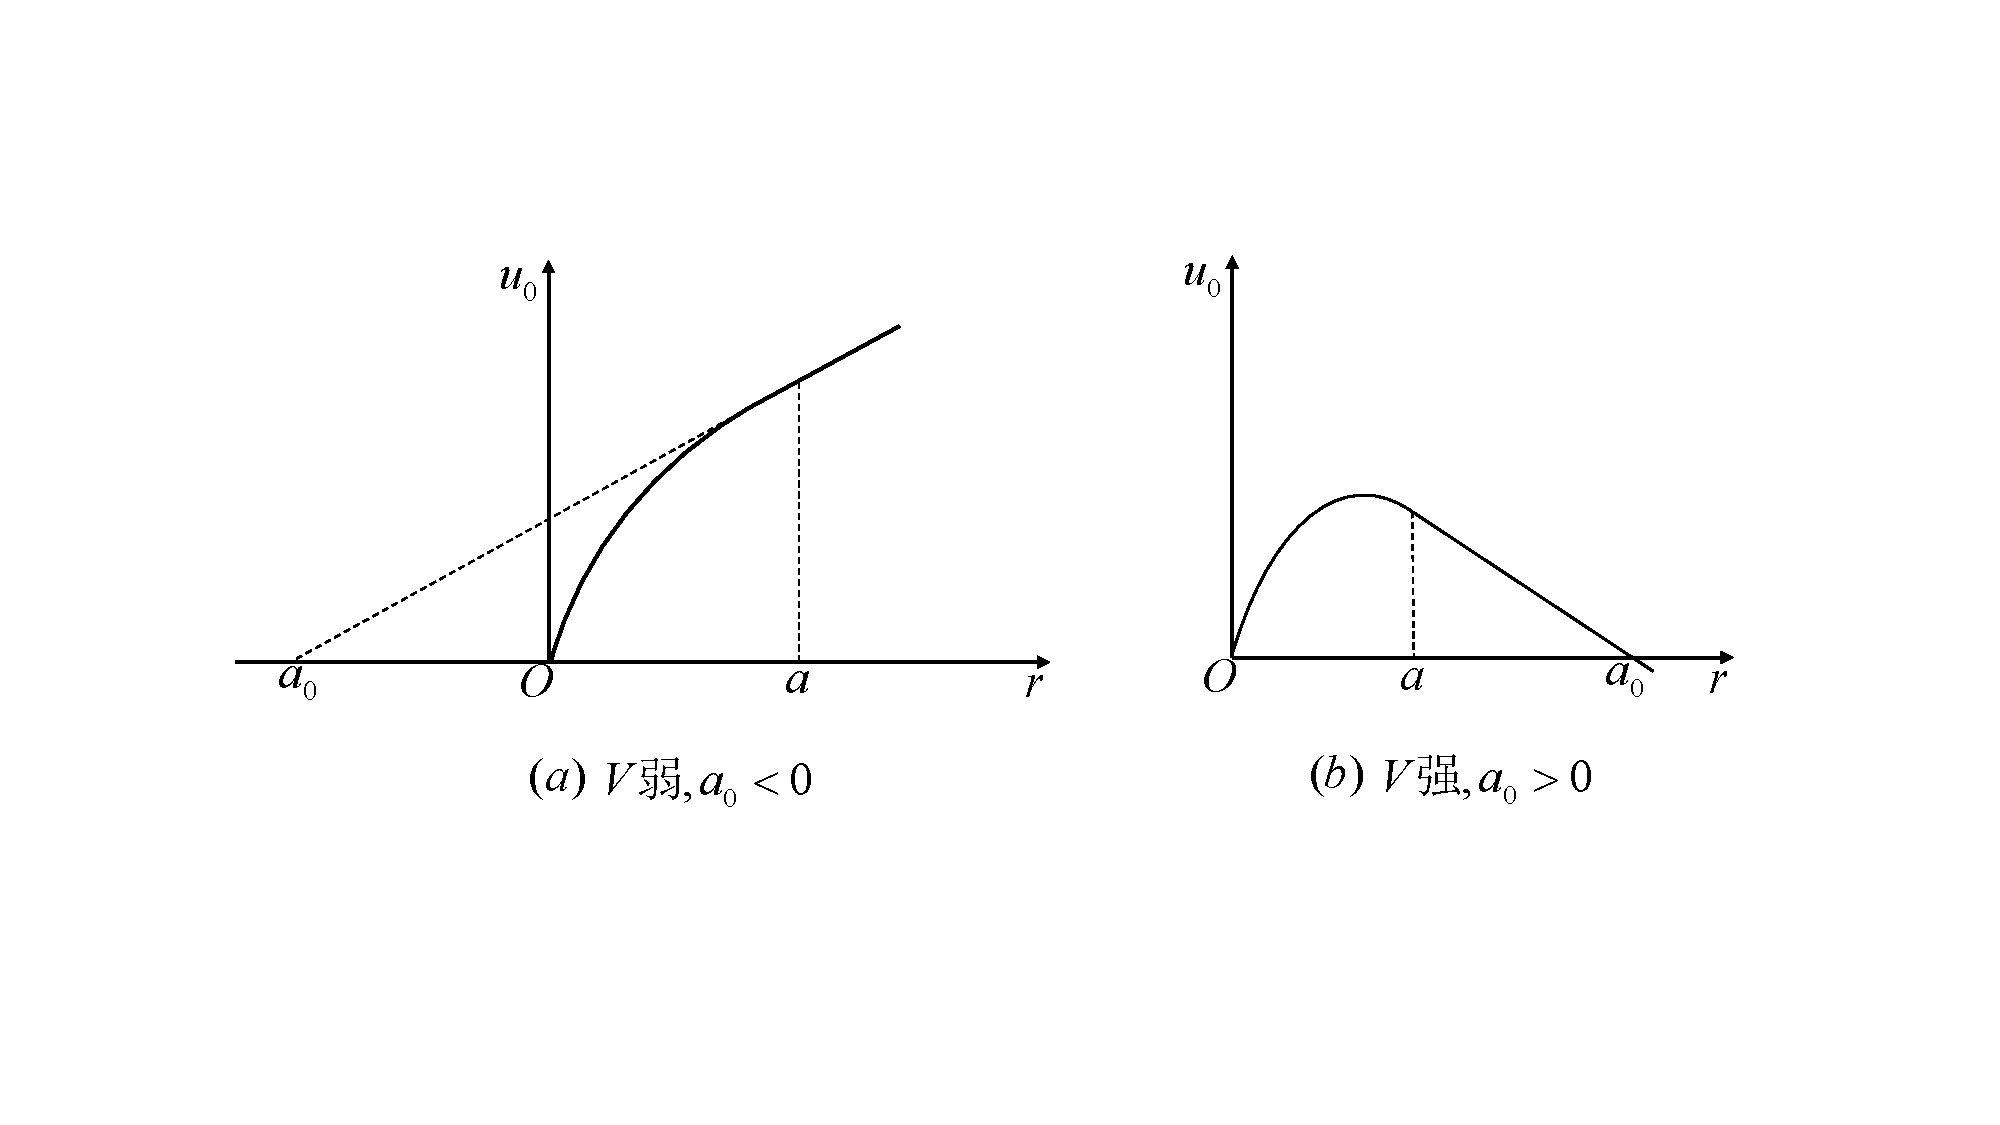
\includegraphics[width=7cm,clip]{QM file/figure/8-4}
	\caption{}\label{fig.8-4}
\end{figure}

下面以势阱$(V<0)$散射为例,说明散射长度的意义.当$E\rightarrow0$,由\eqref{eq83.1}式可知$\frac{u_{0}^{\prime\prime}}{u_{0}}$,$u_{0}$随$r$的变化如图\ref{fig.8-4}所示.如果作用势$V(r)$较弱,以致当$r$达到$a$(作用球半径)时$u_{0}$尚在上升阶段,$u_{0}^{\prime}$为正,则散射长度$a_{0}<0$.这种势阱不能造成束缚态.如果作用势$V(r)$较强,当$r$达到$a$时$u_{0}$已经处于下降阶段,$u_{0}^{\prime}$为负,则散射长度$a_{0}>0$.这种势阱可以造成束缚态能级$(E_{n}<0)$.而$a_{0}=\pm\infty$相当于$r=a$处$u_{0}^{\prime}=0$,这刚好是阱口出现束缚态能级$(E=0_{-})$的条件,这种情况下粒子的入射能量$(E\geqslant0)$接近于阱口附近的束缚态能级,在入射波与阱口束缚态之间容易产生共振跃迁,所以散射截面特别大.
\pskip

\example 讨论球形势阱

\begin{equation}\label{eq83.12}
	V(r)=
	\begin{cases}
		-V_{0},	& r<a	\\
		0,	& r>a
	\end{cases}
\end{equation}
造成的低能$(ka\ll1)$s波$(l=0)$散射.

\solution 令
\begin{empheq}{equation}\label{eq83.13}
	k=\frac{\sqrt{2\mu E}}{\hbar},\quad k_{0}=\frac{\sqrt{2\mu V_{0}}}{\hbar}
\end{empheq}
在阱内$(r<a)$,s波径向方程为
\eqshort
\begin{empheq}{equation}\label{eq83.14}
	u_{0}^{\prime\prime}+(k^{2}+k_{0}^{2})u_{0}=0
\end{empheq}\eqnormal
边界条件为$u_{0}(r=0)=0$.当$E\rightarrow0(k\rightarrow0)$,满足边界条件的解是
\begin{empheq}{equation}\label{eq83.15}
	u_{0}(r)=A\sin k_{0}r\quad (E\rightarrow0,r<a)
\end{empheq}
在阱外$(r>a)$,径向方程为
\eqshort
\begin{empheq}{equation*}
	u_{0}^{\prime\prime}+k^{2}u_{0}=0
\end{empheq}\eqnormal
当$E\rightarrow0$,解为
\begin{empheq}{equation}\label{eq83.16}
	u_{0}(r)=c\bigg(1-\frac{r}{a_{0}}\bigg)\quad (E\rightarrow0,r>a)
\end{empheq}
在$r=a$处,$\frac{u_{0}}{u_{0}^{\prime}}$应该连续,据此求出
\begin{empheq}{align}\label{eq83.17}
	\frac{1}{k}&\tan k_{0}a=a-a_{0}	\nonumber\\
	a_{0}=&-\frac{a(\tan k_{0}a-k_{0}a)}{k_{0}a}
\end{empheq}
$a_{0}$即散射长度.如$a_{0}$有限,由\eqref{eq83.8}式就得到散射截面(与$E$无关).

讨论:(i) 如势阱的性质($V_{0}$及$a$值)刚好使$\tan k_{0}a=k_{0}a$,这时$a_{0}=0$,低能极限下$(E\rightarrow0)\sigma_{\text{总}}\rightarrow0$,势阱是“透明”的.


(ii) 如势阱深而宽,$k_{0}a\gg 1$,同时$\tan k_{0}a$并不太大(非共振散射),这时$a_{0}=a,\sigma_{\text{总}}\approx4\pi a^{2}$,势阱的低能散射效果类似于刚球.


(iii) 如果$k_{0}a=\bigg(n+\frac{1}{2}\bigg)\pi(n=0,1,2,\cdots)$则当$E\rightarrow0$时出现共振散射$(a_{0}=\pm\infty)$.这时阱内区域粒子的德布罗意波长$\lambda_{0}\bigg(\approx\frac{2\pi}{k_{0}}\bigg)$与势阱半径$a$有关系
\eqshort
\begin{empheq}{equation}\label{eq83.18}
	2a=\bigg(n+\frac{1}{2}\bigg)\lambda_{0}
\end{empheq}\eqnormal
这也就是阱口出现束缚能级$(E=0_{-})$的条件.

(iv) 如果势阱浅而窄,$k_{0}a\ll 1$,则可取
\begin{empheq}{equation*}
	\tan k_{0}a\approx k_{0}a+\frac{1}{3}(k_{0}a)^{3}
\end{empheq}
由\eqref{eq83.17}式求得散射长度为
\begin{empheq}{equation}\label{eq83.19}
	a_{0}\approx -\frac{a}{3}(k_{0}a)^{2}=-\frac{2\mu V_{0}a^{3}}{3\hbar^{2}}
\end{empheq}
再由\eqref{eq83.7}式、\eqref{eq83.8}式得出
\begin{empheq}{align}
	\delta_{0}&=-k_{0}a=\bigg(\frac{2\mu V_{0}a^{2}}{3\hbar^{2}}\bigg)ak		\label{eq83.20}\\
	\sigma_{\text{总}}&=4\pi a_{0}^{2}=\frac{16\pi}{9}\bigg(\frac{\mu V_{0}a^{3}}{\hbar^{2}}\bigg)^{2}		\label{eq83.21}
\end{empheq}
如直接利用$\delta_{l}$的近似公式[\eqref{eq82.26}式],也可得到同样的结果.









% 玻恩近似
\section[玻恩近似]{玻恩近似} \label{sec:08.04} % 
% \makebox[5em][s]{} % 短题目拉间距

在弹性散射问题中,波函数表示成入射波和散射波的叠加,即
\begin{empheq}{equation}\label{eq84.1}
	\varPsi=e^{ikz}+\varPsi_{s}
\end{empheq}
$\varPsi$满足定态薛定谔方程,它可以写成
\begin{empheq}{equation}\label{eq84.2}
	(\nabla^{2}+k^{2})\varPsi=\frac{2\mu}{\hbar^{2}}V(\boldsymbol{r})\varPsi
\end{empheq}
其中$k=\frac{\sqrt{2\mu E}}{\hbar}$.\eqref{eq84.1}式中$e^{ikz}$为入射波,$\varPsi_{s}$为散射波,在$r\rightarrow\infty$处$\varPsi_{s}$取球面出射波的形式,即
\begin{empheq}{equation}\label{eq84.3}
	\varPsi_{s}\approx f(\theta,\varphi)\frac{e^{ikr}}{r}\quad (r\rightarrow\infty)
\end{empheq}
上式可以认为是$r\rightarrow\infty$处$\varPsi_{s}$满足的边界条件.

如作用势$V(r)$较弱,以致在作用球内就有$|\varPsi_{s}|<|e^{ikz}|$,我们可以视$V$为微扰,而对\eqref{eq84.2}式采用逐级近似解法.

{\heiti 1. 近似展开}

将总波函数$\varPsi$分解成零级近似,一级修正,二级修正,等等,令
\begin{empheq}{equation}\label{eq84.4}
	\varPsi=\varPsi^{(0)}+\varPsi^{(1)}+\varPsi^{(2)}+\cdots
\end{empheq}
零级近似取为入射波,即
\eqshort
\begin{empheq}{equation}\label{eq84.5}
	\varPsi^{(0)}=e^{ikz}
\end{empheq}\eqnormal
而散射波就是\eqref{eq84.4}式中其余各项之和,即
\begin{empheq}{equation}\label{eq84.6}
	\varPsi_{s}=\varPsi^{(1)}+\varPsi^{(2)}+\cdots
\end{empheq}
在$r\rightarrow\infty$处,各级修正项均应该取球面出射波的形式,即
\begin{empheq}{equation}\label{eq84.7}
	\begin{aligned}
		\varPsi^{(1)} &\approx f^{(1)}(\theta,\varphi)\frac{e^{ikr}}{r}	\\
		\varPsi^{(2)} &\approx f^{(2)}(\theta,\varphi)\frac{e^{ikr}}{r}
	\end{aligned}\qquad (r\rightarrow\infty)
\end{empheq}
等等与\eqref{eq84.3}式、\eqref{eq84.6}式比较,显然有
\begin{empheq}{equation}\label{eq84.8}
	f(\theta,\varphi)=f^{(1)}+f^{(2)}+\cdots
\end{empheq}
$f^{(1)}$和$f^{(2)}$就是散射振幅的一级近似和二级修正.

入射波$\varPsi^{(0)}$满足方程
\eqshort
\begin{empheq}{equation}\label{eq84.9}
	(\nabla^{2}+k^{2})\varPsi^{(0)}=0
\end{empheq}\eqnormal
因此\eqref{eq84.2}式化成
\eqindent{1}
\begin{empheq}{equation}\label{eq84.10}
	(\nabla^{2}+k^{2})(\varPsi^{(1)}+\varPsi^{(2)}+\cdots)=\frac{2\mu}{\hbar^{2}}V(\boldsymbol{r})(\varPsi^{(0)}+\varPsi^{(1)}+\varPsi^{(2)}+\cdots)
\end{empheq}\eqnormal
对上式用逐级近似解法,可令
\begin{empheq}{align}
	(\nabla^{2}+k^{2})\varPsi^{(1)}&=\frac{2\mu}{\hbar^{2}}V\varPsi^{(0)}		\label{eq84.11}	\\
	(\nabla^{2}+k^{2})\varPsi^{(2)}&=\frac{2\mu}{\hbar^{2}}V\varPsi^{(1)}		\label{eq84.12}
\end{empheq}
等等,先由\eqref{eq84.11}式解出$\varPsi^{(1)}$,再代入\eqref{eq84.12}式解出$\varPsi^{(2)}\cdots\cdots$依次逐级求解.

{\heiti 2. 格林函数}

\eqref{eq84.11}式的形式解可以写成
\begin{empheq}{equation*}\label{eq84.11'}
	\varPsi^{(1)}(\boldsymbol{r})=\frac{2\mu}(\nabla^{2}+k^{2})^{-1}V(\boldsymbol{r})\varPsi^{(0)}(\boldsymbol{r})
	\tag{$8.4.11^{\prime}$}
\end{empheq}
这里$(\nabla^{2}+k^{2})^{-1}$按照算符来理解,但其性质有待明确.引入$\delta$函数$\delta(\boldsymbol{r}-\boldsymbol{r}^{\prime})$,规定其性质为(这里和以下,凡是三重积分均指“全空间”积分)
\begin{empheq}{equation}\label{eq84.13}
	\int\rho(\boldsymbol{r}^{\prime})\delta(\boldsymbol{r}-\boldsymbol{r}^{\prime})d^{3}\boldsymbol{r}^{\prime}=\rho(\boldsymbol{r})
\end{empheq}
$\rho(\boldsymbol{r})$为任何具有良好积分收敛性的连续函数.再引入格林函数
\begin{empheq}{equation}\label{eq84.14}
	G(\boldsymbol{r},\boldsymbol{r}^{\prime})=(\nabla^{2}+k^{2})^{-1}\delta(\boldsymbol{r}-\boldsymbol{r}^{\prime})
\end{empheq}
则有
\begin{empheq}{align}\label{eq84.15}
	\int& G(\boldsymbol{r},\boldsymbol{r}^{\prime})\rho(\boldsymbol{r}^{\prime})d^{3}\boldsymbol{r}^{\prime}	\nonumber\\
	&=(\nabla^{2}+k^{2})^{-1}\int\delta(\boldsymbol{r}-\boldsymbol{r}^{\prime})\rho(\boldsymbol{r}^{\prime})d^{3}\boldsymbol{r}^{\prime}	\nonumber\\
	&=(\nabla^{2}+k^{2})^{-1}\rho(\boldsymbol{r})
\end{empheq}
因此\eqref{eq84.11'}式形式上可以写成
\begin{empheq}{equation}\label{eq84.16}
	\boxed{\varPsi^{(1)}(\boldsymbol{r})=\frac{2\mu}{\hbar^{2}}\int G(\boldsymbol{r},\boldsymbol{r}^{\prime})V(\boldsymbol{r}^{\prime})\varPsi^{(0)}(\boldsymbol{r}^{\prime})d^{3}\boldsymbol{r}^{\prime}}
\end{empheq}
注意,\eqref{eq84.14}式仅是格林函数的形式定义,其实质就是
\begin{empheq}{equation}\label{eq84.14'}
	(\nabla^{2}+k^{2})G(\boldsymbol{r},\boldsymbol{r}^{\prime})=\delta(\boldsymbol{r}-\boldsymbol{r}^{\prime})
	\tag{$8.4.14^{\prime}$}
\end{empheq}
将齐次方程$(\nabla^{2}+k^{2})u=0$的任何一个解加入$G(\boldsymbol{r},\boldsymbol{r}^{\prime})$中,显然仍满足\eqref{eq84.14'}式.在具体问题中,选取$G(\boldsymbol{r},\boldsymbol{r}^{\prime})$的函数形式时应该根据问题的性质,并满足相应的边界条件.对于散射问题,可取
\begin{empheq}{equation}\label{eq84.17}
	\delta(\boldsymbol{r}-\boldsymbol{r}^{\prime})=\frac{1}{(2\pi)^{3}}\int\exp[i\boldsymbol{k}^{\prime}\cdot(\boldsymbol{r}-\boldsymbol{r}^{\prime})]d^{3}\boldsymbol{k}^{\prime}
\end{empheq}
由于
\begin{empheq}{equation*}
	(\nabla^{2}+k^{2})e^{i\boldsymbol{k}^{\prime}\cdot\boldsymbol{r}}=(k^{2}-k^{\prime2})e^{i\boldsymbol{k}^{\prime}\cdot\boldsymbol{r}}
\end{empheq}
格林函数可以取为
\eqlong
\begin{empheq}{equation}\label{eq84.18}
	G(\boldsymbol{r},\boldsymbol{r}^{\prime})=\frac{1}{(2\pi)^{3}}\int\frac{d^{3}\boldsymbol{k}^{\prime}}{k^{2}-k^{\prime2}}\exp[i\boldsymbol{k}^{\prime}\cdot(\boldsymbol{r}-\boldsymbol{r}^{\prime})]
\end{empheq}\eqnormal
上式中积分在$\boldsymbol{k}^{\prime}$空间进行,$k,\boldsymbol{r},\boldsymbol{r}^{\prime}$作为参量对待.如在$\boldsymbol{k}^{\prime}$空间取球坐标$(k^{\prime},\theta,\varphi)$,并以$(\boldsymbol{r}-\boldsymbol{r}^{\prime})$作为极轴,则
\begin{empheq}{equation*}
	d^{3}\boldsymbol{k}^{\prime}=k^{\prime2}dk^{\prime}\sin\theta d\theta d\varphi
\end{empheq}
\eqref{eq84.18}式中角部积分容易算出,为
\begin{empheq}{align}\label{eq84.19}
	\int&\exp[i\boldsymbol{k}^{\prime}\cdot(\boldsymbol{r}-\boldsymbol{r}^{\prime})]\sin\theta d\theta d\varphi		\nonumber\\
	&=\int_{0}^{2\pi}d\varphi\int_{0}^{\pi}\exp[ik^{\prime}|\boldsymbol{r}-\boldsymbol{r}^{\prime}|\cos\theta]\sin\theta d\theta	\nonumber\\
	&=4\pi\frac{\sin(k^{\prime}|\boldsymbol{r}-\boldsymbol{r}^{\prime}|)}{k^{\prime}|\boldsymbol{r}-\boldsymbol{r}^{\prime}|}
\end{empheq}
代入\eqref{eq84.18}式,得到
\eqindent{1}
\begin{empheq}{align}\label{eq84.20}
	G&(\boldsymbol{r},\boldsymbol{r}^{\prime})=\frac{1}{2\pi^{2}}\cdot\frac{1}{|\boldsymbol{r}-\boldsymbol{r}^{\prime}|}\int_{0}^{\infty}\frac{k^{\prime}dk^{\prime}}{k^{2}-k^{\prime}}\sin(k^{\prime}|\boldsymbol{r}-\boldsymbol{r}^{\prime}|)	\nonumber\\
	&=\frac{i}{8\pi^{2}|\boldsymbol{r}-\boldsymbol{r}^{\prime}|}\int_{-\infty}^{\infty}\bigg(\frac{1}{k^{\prime}+k}+\frac{1}{k^{\prime}-k}\bigg)\exp(ik^{\prime}|\boldsymbol{r}-\boldsymbol{r}^{\prime}|)dk^{\prime}
\end{empheq}\eqnormal

\begin{figure}[!h]
	\centering
	\small
	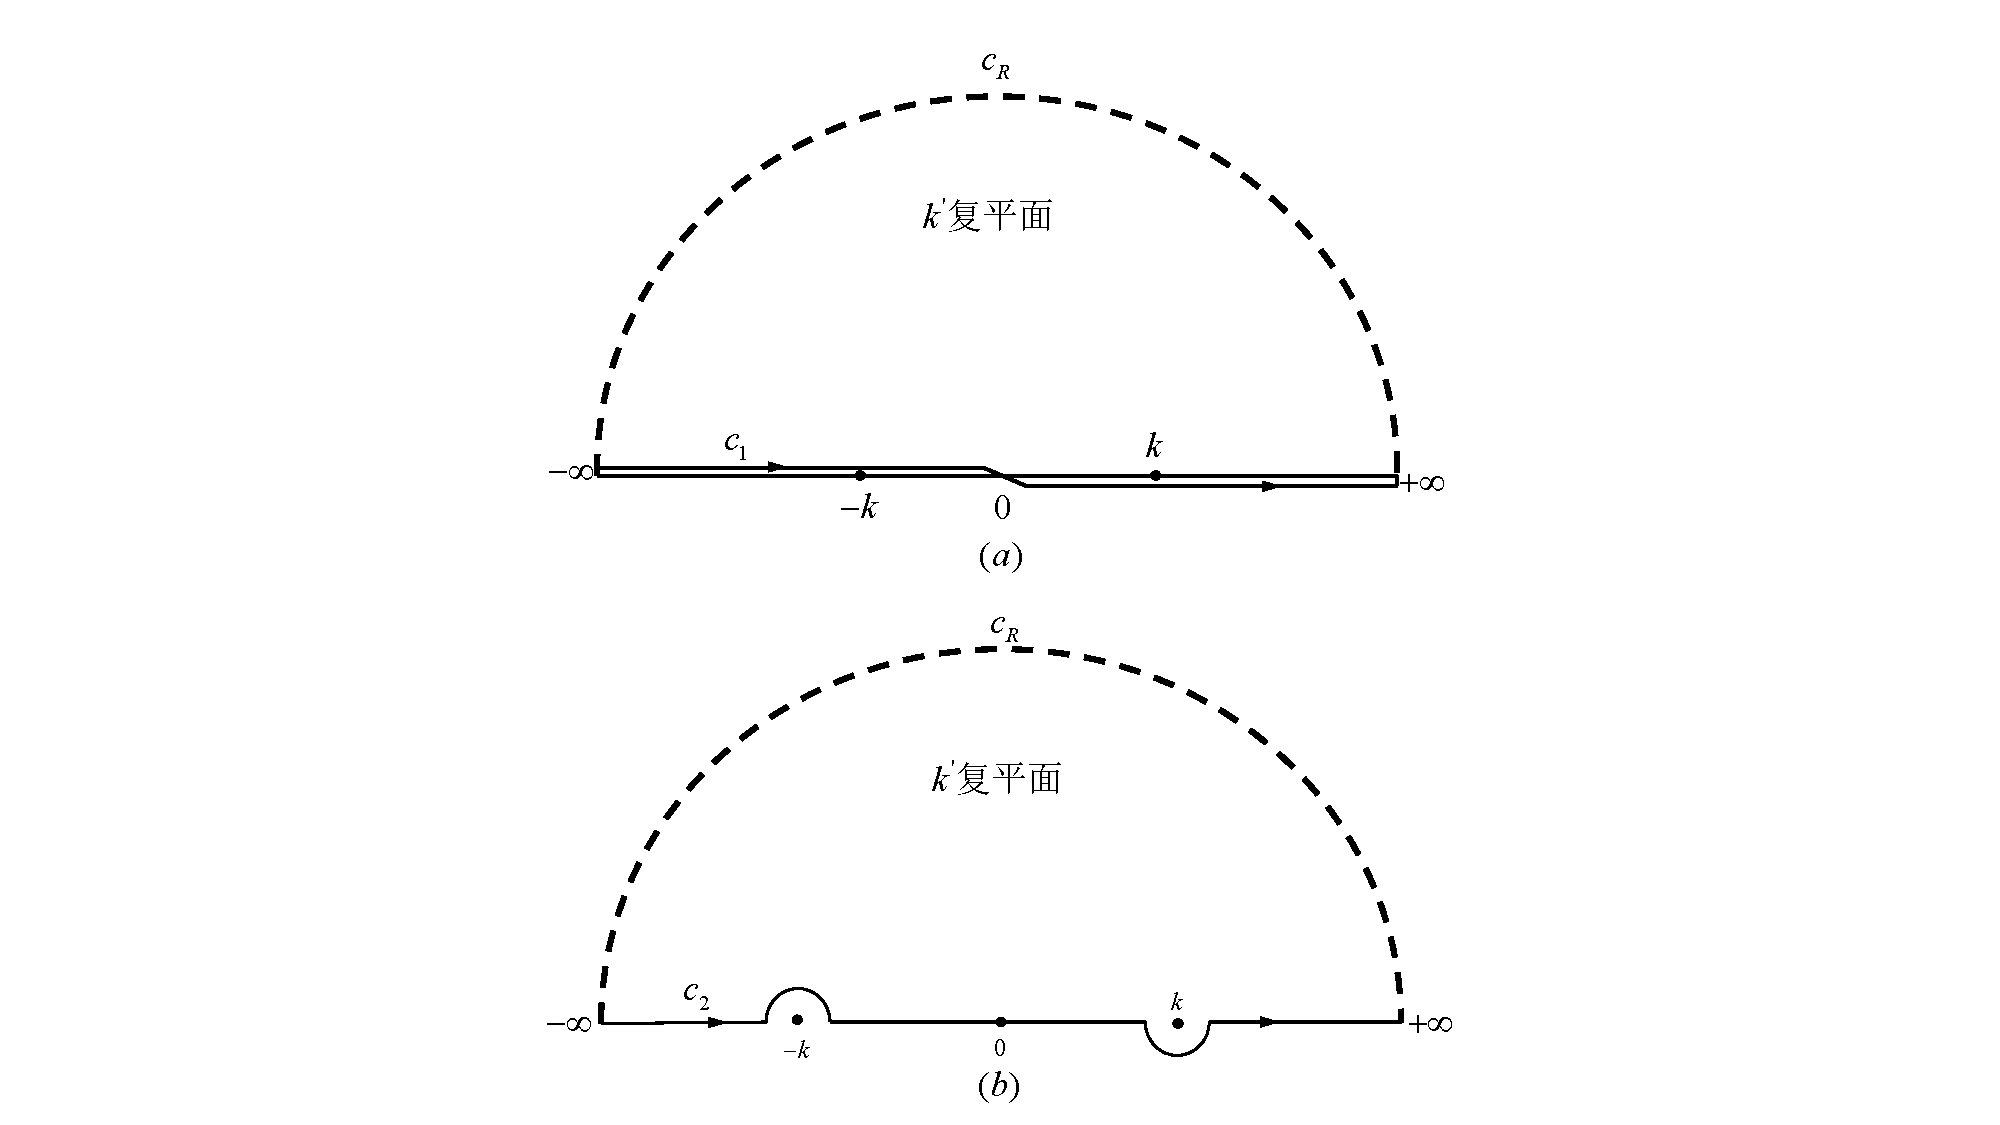
\includegraphics[width=5.5cm,clip]{QM file/figure/8-5}
	\caption{}\label{fig.8-5}
\end{figure}
上式可用$\boldsymbol{k}^{\prime}$复平面上围道积分法算出.但$k^{\prime}=\pm k$是被积函数的一级极点,为了确保$G(\boldsymbol{r},\boldsymbol{r}^{\prime})$中只有出射波,[这样才能符合边界条件\eqref{eq84.7}式]在$\boldsymbol{k}^{\prime}$复平面的左半,积分路线应取实轴上岸,在$\boldsymbol{k}^{\prime}$复平面的右半,积分路线应取实轴下岸,如图\ref{fig.8-5}(a)所示,亦即\eqref{eq84.20}式中积分路线规定为
\begin{empheq}{equation}\label{eq84.21}
	\int_{-\infty}^{\infty}\cdots dk^{\prime}\Rightarrow\int_{c_{1}}\cdots dk^{\prime}
\end{empheq}
这个规定等价于\eqref{eq84.20}式中$k$换成$k+i\varepsilon$($\varepsilon$为无限小正实数) ,或等价于沿图\ref{fig.8-5}(b)中路径$c_{2}$的积分.注意,图\ref{fig.8-5}中沿大圆弧$c_{R}$的积分为0.按照复平面围道积分的残数定理,容易算出
\begin{empheq}{equation}\label{eq84.22}
	\boxed{G(\boldsymbol{r},\boldsymbol{r}^{\prime})=-\frac{\exp(ik|\boldsymbol{r}-\boldsymbol{r}^{\prime}|)}{4\pi|\boldsymbol{r}-\boldsymbol{r}^{\prime}|}}
\end{empheq}
这正是符合散射波性质的出射波形式格林函数.反之,如取积分路径为图\ref{fig.8-5}中(a)实轴下岸及(b)实轴上岸,[相当于\eqref{eq84.20}式中$k$换成$k+i\varepsilon$]则给出
\begin{empheq}{equation*}
	G(\boldsymbol{r},\boldsymbol{r}^{\prime})=-\frac{\exp(ik|\boldsymbol{r}-\boldsymbol{r}^{\prime}|)}{4\pi|\boldsymbol{r}-\boldsymbol{r}^{\prime}|}
\end{empheq}
就不符合散射波的性质,不能采用.


{\heiti 3. 玻恩近似}

将格林函数\eqref{eq84.22}式代入\eqref{eq84.16}式,得到$\varPsi^{(1)}$的明显表示式
\eqlong
\begin{empheq}{equation}\label{eq84.23}
	\varPsi^{(1)}=-\frac{\mu}{2\pi\hbar^{2}}\int\frac{\exp(ik|\boldsymbol{r}-\boldsymbol{r}^{\prime}|)}{|\boldsymbol{r}-\boldsymbol{r}^{\prime}|}V(\boldsymbol{r}^{\prime})\varPsi^{(0)}(\boldsymbol{r}^{\prime})d^{3}\boldsymbol{r}^{\prime}
\end{empheq}\eqnormal
为了得到散射振幅的一级近似$f^{(1)}$,只需要求出$r\rightarrow\infty$处$\varPsi^{(1)}$的函数形式,由于$r\gg r^{\prime}$,可以取下列近似(参看图\ref{fig.8-6}):
\begin{empheq}{equation}\label{eq84.24}
	k|\boldsymbol{r}-\boldsymbol{r}^{\prime}|\approx k\bigg(r-\frac{\boldsymbol{r}^{\prime}\cdot\boldsymbol{r}}{r}\bigg)=kr-\boldsymbol{k}\cdot\boldsymbol{r}^{\prime}
\end{empheq}

\begin{figure}[!h]
	\centering
	\small
	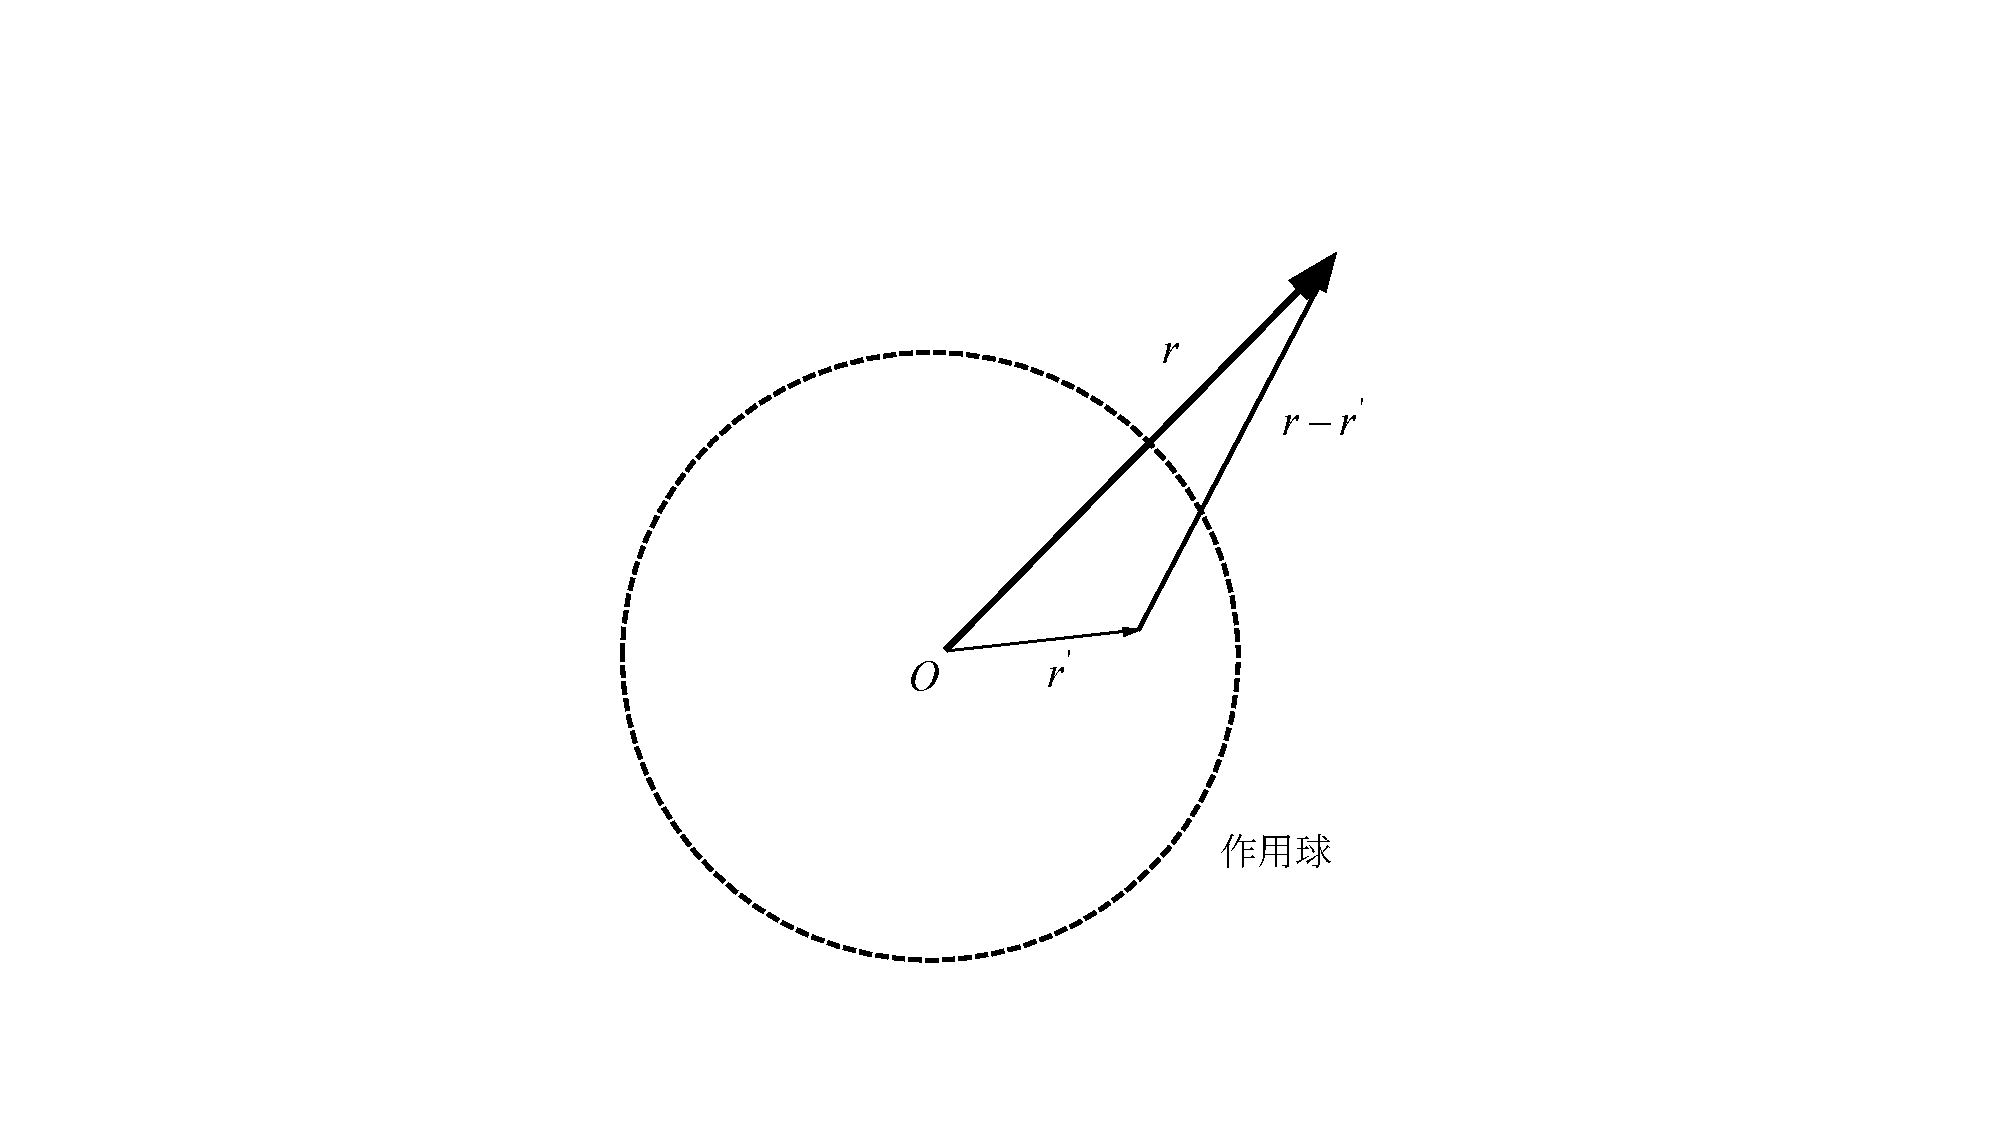
\includegraphics[width=5cm,clip]{QM file/figure/8-6}
	\caption{}\label{fig.8-6}
\end{figure}
$\boldsymbol{k}$为出射波波矢量,其方向即$\boldsymbol{r}$的方向,$\boldsymbol{k}=k\frac{\boldsymbol{r}}{r}$.对于\eqref{eq84.5}式及\eqref{eq84.23}式中的入射波波函数,可表示成
\begin{empheq}{align*}
	\varPsi^{(0)(\boldsymbol{r})}&=e^{ikz}=e^{i\boldsymbol{k}_{0}\cdot\boldsymbol{r}}	\tag{$8.4.5^{\prime}$}\label{eq84.5'}\\
	\varPsi^{(0)(\boldsymbol{r}^{\prime})}&=e^{ikz^{\prime}}=e^{i\boldsymbol{k}_{0}\cdot\boldsymbol{r}^{\prime}}	\tag{$8.4.5^{\prime\prime}$}\label{eq84.5''}\\
\end{empheq}
\noindent$k_{0}$为入射波波矢量,其方向即$z$轴及$z^{\prime}$轴方向.将\eqref{eq84.24}式及\eqref{eq84.5''}式代入\eqref{eq84.23}式,并取\eqref{eq84.23}式中分母$|\boldsymbol{r}-\boldsymbol{r}^{\prime}|$$\approx r$,得到
\eqlong
\begin{empheq}{align}\label{eq84.25}
	\varPsi^{(1)}(\boldsymbol{r}) &\approx-\frac{\mu}{2\pi\hbar^{2}}\frac{e^{ikr}}{r}\int V(\boldsymbol{r}^{\prime})\exp[i(\boldsymbol{k_{0}}-\boldsymbol{k})\cdot\boldsymbol{r}^{\prime}]d^{3}\boldsymbol{r}^{\prime}	\nonumber\\
	&=-\frac{\mu}{2\pi\hbar^{2}}V(\boldsymbol{k},\boldsymbol{k_{0}})\frac{e^{ikr}}{r}
\end{empheq}
\eqnormal
其中
\begin{empheq}{equation}\label{eq84.26}
	V(\boldsymbol{k},\boldsymbol{k_{0}})=\int V(\boldsymbol{r}^{\prime})\exp[i(\boldsymbol{k_{0}}-\boldsymbol{k})\cdot\boldsymbol{r}^{\prime}]d^{3}\boldsymbol{r}^{\prime}
\end{empheq}
比较\eqref{eq84.7}式及\eqref{eq84.25}式,即得散射振幅的一级近似:
\begin{empheq}{equation}\label{eq84.27}
	\boxed{f^{(1)}(\theta,\varphi)=-\frac{\mu}{2\pi\hbar^{2}}V(\boldsymbol{k},\boldsymbol{k_{0}})	}
\end{empheq}
$\boldsymbol{k}$的方向即$(\theta,\varphi)$方向.$(\hbar\boldsymbol{k}-\hbar\boldsymbol{k_{0}})$是散射过程中粒子的动量变化,常被称为“动量转移”,记为$\hbar q$,即
\begin{empheq}{equation}\label{eq84.28}
	\boxed{\boldsymbol{q}=\boldsymbol{k}-\boldsymbol{k_{0}},\quad q=2k\sin\frac{\theta}{2}	}
\end{empheq}

\begin{wrapfigure}[9]{r}{8em}
	\centering
	\small
	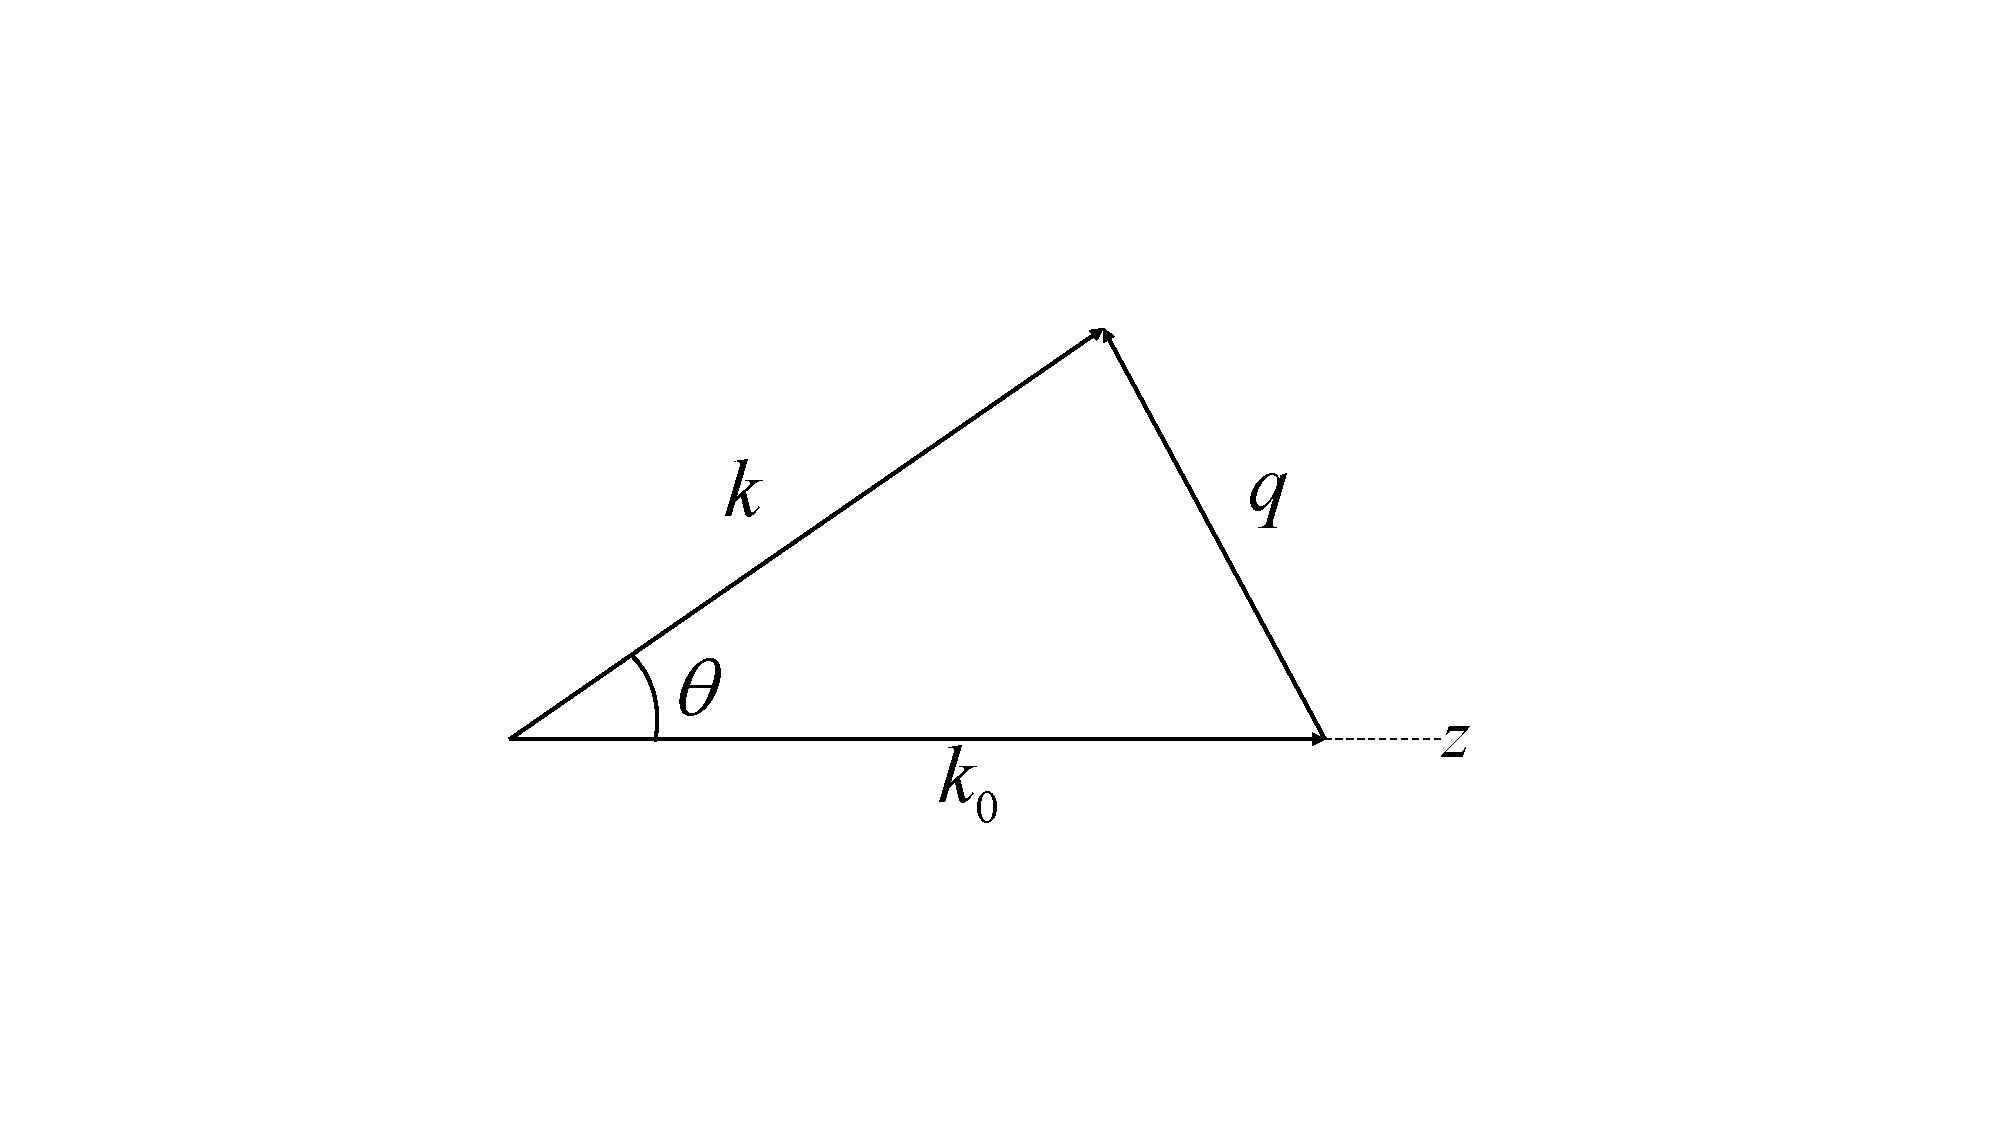
\includegraphics[width=3cm,clip]{QM file/figure/8-7}
	\caption{}\label{fig.8-7}
\end{wrapfigure}
如图\ref{fig.8-7}所示,用$\boldsymbol{q}$代替$(\boldsymbol{k}-\boldsymbol{k_{0}})$,\eqref{eq84.26}式可以写成
\eqindent{4}
\begin{empheq}{equation*}\label{eq84.26'}
	V(\boldsymbol{k},\boldsymbol{k_{0}})=\int V(\boldsymbol{r}^{\prime})	e^{-i\boldsymbol{q}\cdot\boldsymbol{r}^{\prime}}	d^{3}\boldsymbol{r}^{\prime}	\tag{$8.4.26^{\prime}$}
\end{empheq}\eqnormal

如果是中心力散射,$V(\boldsymbol{r}^{\prime})=V(r^{\prime})$,\eqref{eq84.26'}式中角部积分与$V$无关,可以直接算出,如下.$\boldsymbol{r}^{\prime}$空间用球坐标,并以$-\boldsymbol{q}$方向作为极轴方向,则$$-\boldsymbol{q}\cdot\boldsymbol{r}^{\prime}=qr^{\prime}\cos\theta^{\prime},\quad d^{3}\boldsymbol{r}^{\prime}=r^{\prime2}dr^{\prime}\sin\theta^{\prime}d\theta^{\prime}d\varphi^{\prime}$$
\eqlong
\begin{empheq}{align}\label{eq84.29}
	\int e^{-i\boldsymbol{q}\cdot\boldsymbol{r}^{\prime}}\sin\theta^{\prime}d\theta^{\prime}d\varphi&=2\pi\int_{0}^{\pi}e^{iqr^{\prime}\cos\theta^{\prime}}\sin\theta^{\prime}d\theta^{\prime}	\nonumber\\
	&=\frac{4\pi}{qr^{\prime}}\sin qr^{\prime}
\end{empheq}\eqnormal
因此
\begin{empheq}{equation}\label{eq84.30}
	V(\boldsymbol{k},\boldsymbol{k_{0}})=4\pi\int_{0}^{\infty}V(r^{\prime})\frac{\sin qr^{\prime}}{qr^{\prime}}r^{\prime2}dr^{\prime}
\end{empheq}
\begin{empheq}{equation}\label{eq84.31}
	\boxed{f^{(1)}(\theta)=-\frac{2\mu}{\hbar^{2}}\int_{0}^{\infty}V(r^{\prime})\frac{\sin qr^{\prime}}{qr^{\prime}}r^{\prime2}dr^{\prime}	}
\end{empheq}
由于$q=2k\sin\bigg(\frac{\theta}{2}\bigg)$,所以$f^{(1)}$是散射角$\theta$的函数.

如果略去二级修正,则微分散射截面为
\begin{empheq}{equation}\label{eq84.32}
	\sigma(\theta,\varphi)\approx|f^{(1)}|^{2}=\frac{\mu^{4}}{4\pi^{2}\hbar^{4}}|V(\boldsymbol{k},\boldsymbol{k_{0}})|^{2}
\end{empheq}
对于中心力场散射,微分散射截面仅为$\theta$的函数,
\begin{empheq}{equation}\label{eq84.33}
	\sigma(\theta)\approx\frac{4\mu^{2}}{\hbar^{4}}\bigg[\int_{0}^{\infty}V(r^{\prime})\frac{\sin qr^{\prime}}{qr^{\prime}}r^{\prime2}dr^{\prime}\bigg]^{2}
\end{empheq}
以上结果[主要指\eqref{eq84.25}、\eqref{eq84.27}、\eqref{eq84.32}式]通常称为玻恩(M.Born)近似.

{\heiti 4. 玻恩近似的适用条件}

\eqref{eq84.2}式或\eqref{eq84.10}式的严格解应该写成
\begin{empheq}{align*}\label{eq84.10'}
	\varPsi_{s}(\boldsymbol{r}) &=(\nabla^{2}+k^{2})^{-1}\frac{2\mu}{\hbar^{2}}V(\boldsymbol{r})\varPsi(\boldsymbol{r})	\\
	&=\frac{2\mu}{\hbar^{2}}\int G(\boldsymbol{r},\boldsymbol{r}^{\prime})V(\boldsymbol{r}^{\prime})\varPsi(\boldsymbol{r}^{\prime})d^{3}\boldsymbol{r}^{\prime}
	\tag{$8.4.10^{\prime}$}
\end{empheq}
由于$\varPsi=\varPsi^{(0)}+\varPsi_{s}$,上式为积分方程\eqref{eq84.16}式是上式的一级近似解,相当于在右端的积分中以$\varPsi^{(0)}$代替$\varPsi$.由此可知\eqref{eq84.16}式和\eqref{eq84.23}式的适用条件是在散射区内$(r\sim r^{\prime})|\varPsi^{(1)}(\boldsymbol{r})|\ll|\varPsi^{(0)}(\boldsymbol{r})|$,亦即
\begin{empheq}{equation}\label{eq84.34}
	|\varPsi^{(1)}(\boldsymbol{r})|\ll1\quad (r\sim r^{\prime})
\end{empheq}
通常,作用势$V(\boldsymbol{r}^{\prime})$总是存在一定的有效范围(作用球,半径$a$),在作用球内,$V$变化平缓,在作用球外,$V$迅速减弱.作为数量级估算,\eqref{eq84.23}式中$V(\boldsymbol{r}^{\prime})$不妨用平均值$V_{0}$来代替,而积分在作用球内进行.这样做相当于采用球形势垒(阱)模型.通常,在力心附近$(r\sim 0)$散射作用较强,所以\eqref{eq84.34}式可取$r=0$进行估算,即适用条件取为
\eqlong
\begin{empheq}{equation}\label{eq84.35}
	|\varPsi^{(1)}(0)|\approx\frac{\mu|V_{0}|}{2\pi\hbar^{2}}\bigg|\int\frac{d^{3}\boldsymbol{r}^{\prime}}{r^{\prime}}\exp[ikr^{\prime}+i\boldsymbol{k_{0}}\cdot\boldsymbol{r}^{\prime}]\bigg|\ll1
\end{empheq}\eqnormal
其中$\exp(i\boldsymbol{k_{0}}\cdot\boldsymbol{r}^{\prime})=\exp(ikz^{\prime})=\varPsi^{(0)}(\boldsymbol{r}^{\prime})$.

对于低能散射,$ka\ll 1$,\eqref{eq84.35}式中指数函数近似等于1,而
\begin{empheq}{equation*}
	\int\frac{d^{3}\boldsymbol{r}^{\prime}}{r^{\prime}}\approx4\pi\int_{0}^{a}r^{\prime}d^{\prime}=2\pi a^{2}
\end{empheq}
所以适用条件为
\begin{empheq}{equation}\label{eq84.36}
	|\varPsi^{(1)}(0)|\approx \mu|V_{0}|\frac{a^{2}}{\hbar^{2}}\ll1
\end{empheq}
要满足此式,势垒(阱)必须充分弱($|V_{0}|$小)而窄($a$小).

对于高能散射,$ka\gg1$,\eqref{eq84.35}式中指数函数在$0<r^{\prime}<a$范围内将多次振荡,必须作出较精确的估算,采用球坐标$(r^{\prime},\theta^{\prime},\varphi^{\prime})$,将\eqref{eq84.35}式中角部积分算出[参看\eqref{eq84.29}式],
\begin{empheq}{equation*}
	\int e^{i\boldsymbol{k}_{0}\cdot\boldsymbol{r}}\sin\theta^{\prime}d\varphi^{\prime}=4\pi\frac{\sin kr^{\prime}}{kr^{\prime}}
\end{empheq}
所以
\eqlong
\begin{empheq}{align}\label{eq84.37}
	&\int\frac{d^{3}\boldsymbol{r}^{\prime}}{r^{\prime}}\exp(ikr^{\prime}+i\boldsymbol{k_{0}}\cdot\boldsymbol{r}^{\prime})=\frac{4\pi}{k}\int_{0}^{a}\sin kr^{\prime}e^{ikr^{\prime}}dr^{\prime}	\nonumber\\
	=&\frac{4\pi}{k^{2}}\int_{0}^{ak}\sin xe^{ix}dx=\frac{4\pi}{k^{2}}\bigg[\frac{i}{2}ak+\frac{1}{4}(1-e^{2iak})\bigg]	\nonumber\\
	=&\frac{4\pi}{k^{2}}\cdot\frac{i}{2}ak=2i\pi\frac{a}{k}
\end{empheq}\eqnormal
代入\eqref{eq84.35},即得适用条件为
\begin{empheq}{equation}\label{eq84.38}
	|\varPsi^{(1)}(0)|\approx \mu|V_{0}|\frac{a}{\hbar^{2}k}\ll1
\end{empheq}
即
\begin{empheq}{equation*}\label{eq84.38'}
	\mu|V_{0}|\frac{a^{2}}{\hbar^{2}}\ll ak\quad\text{或}\quad 2|V_{0}|ak\ll\frac{\hbar^{2}k^{2}}{2\mu}=E
	\tag{$8.4.38^{\prime}$}
\end{empheq}
显然,入射粒子的动能$\bigg(E=\frac{\hbar^{2}k^{2}}{2\mu}\bigg)$越大,条件\eqref{eq84.38'}越易满足.注意,对于一定的势场$(V_{0},a)$,玻恩近似是否适用于低能散射,即\eqref{eq84.36}式是否成立,是由势场本身决定的;而对于高能散射,只要入射能量足够大,总能使\eqref{eq84.38}式成立,即玻恩近似可以适用.另外,比较\eqref{eq84.36}及\eqref{eq84.38}式,可知$|\varPsi^{(1)}(0)|^{2}$之值在高能散射时约为低能散射时的$(ak)^{-2}$倍,由此可以估计,两种情况下总散射截面大致也相差$(ak)^{-2}$倍.

顺便讨论一下中心力散射的玻恩近似\eqref{eq84.31}、\eqref{eq84.33}式.在低能散射条件$(ka\ll1)$下,对于任何散射$\theta$,均有
\begin{empheq}{align*}
	qr^{\prime}=2kr^{\prime}&\sin\bigg(\frac{\theta}{2}\bigg)<2ka\ll1	\\
	&\frac{\sin qr^{\prime}}{qr^{\prime}}\approx 1
\end{empheq}
\eqref{eq84.31}式给出
\begin{empheq}{equation}\label{eq84.39}
	f^{(1)}\approx -\frac{2\mu}{\hbar^{2}}\int_{0}^{\infty}V(r^{\prime})r^{\prime2}dr^{\prime}
\end{empheq}
$f(\theta)\approx f^{(1)}$与$\theta$无关,这结果相当于分波法中低能s波$(l=0)$散射.例如对于球形势阱$(V=-V_{0},r<a)$,上式给出
\begin{empheq}{align}\label{eq84.40}
	&f(\theta)\approx f^{(1)}\approx\frac{2\mu V_{0}a^{3}}{3\hbar^{2}}		\nonumber\\
	\sigma_{\text{总}}&\approx 4\pi|f|^{2}=\frac{16\pi}{9}\bigg(\frac{\mu V_{0}a^{3}}{\hbar^{2}}\bigg)^{2}
\end{empheq}
这正是\eqref{eq83.21}式.$\S$\ref{sec:08.03}例题中提到的条件$ka\ll1$,正是玻恩近似的适用条件,即本节\eqref{eq84.36}式注意,由于条件\eqref{eq84.36}式,$\sigma_{\text{总}}\ll\pi a^{2}$.

仍以球形势阱(或势垒,强度$V_{0}$,半径$a$)为例,对高能散射作定性讨论.\eqref{eq84.31}式中以$\pm V_{0}$代替$V(r^{\prime})$后,积分可以简单算出,
\eqlong
\begin{empheq}{align}\label{eq84.41}
	&\int_{0}^{a}\frac{\sin qr^{\prime}}{qr^{\prime}}r^{\prime2}dr^{\prime}=q^{-3}\int_{0}^{aq}x\sin xdx		\nonumber\\
	=&a^{3}(\sin aq-aq\cos a)(aq)^{-3}=a^{3}F(aq)
\end{empheq}\eqnormal
其中$a_{q}=2ak\sin\bigg(\frac{\theta}{2}\bigg)$.当$aq<\pi$,$F(aq)$随$aq$之增大而徐缓减小,$(aq=0.1,F=0.33;aq=1,F=0.30;aq=2,F=0.22;aq=\pi,F=0,10)$当$aq>\pi$,$|F(aq)|$迅速减小$(aq=4.49,F\sim0;aq=5,F=-\num{0.019};aq=2\pi,F=-\num{0.025};aq=3\pi,F=\num{0.011})$.因此,仅当$\theta<\pi/ak(aq\sim ak\theta<\pi)$,$f(\theta)$及$\sigma(\theta)$才有显著的值(但对$\theta$的变化不敏感).这就是说,在玻恩近似成立的前提下,大部分散射粒子的散射角$\theta<\frac{\pi}{ak}$.相应的$f(\theta)$约为
\begin{empheq}{align}\label{eq84.42}
	|f(\theta)|\approx \frac{2\mu V_{0}a^{3}}{\hbar^{2}}F(aq)\lesssim\frac{2\mu V_{0}a^{3}}{3\hbar^{2}}
\end{empheq}
$\bigg(F\lesssim\frac{1}{3}\bigg)$而总散射截面约为
\begin{empheq}{align}\label{eq84.43}
	\sigma_{\text{总}} &=\int|f(\theta)|^{2}\sin\theta d\theta d\varphi	\nonumber\\
	&\lesssim\bigg(\frac{2\mu V_{0}a^{3}}{3\hbar^{2}}\bigg)^{2}2\pi\int_{0}^{\frac{\pi}{ak}}\sin\theta d\theta	\nonumber\\
	&\sim \bigg(\frac{2\mu V_{0}a^{3}}{3\hbar^{2}}\bigg)\frac{\pi^{3}}{(ak)^{2}}\propto\frac{1}{k^{2}}\propto\frac{1}{E}
\end{empheq}
按量级说,大致是低能$\sigma_{\text{总}}$的$(ak)^{-2}$倍.注意,由于条件\eqref{eq84.38'}式,易见$\sigma_{\text{总}}\ll4\pi a^{2}$,这意味着散射是微弱的.而且,$\sigma_{\text{总}}$大体上与$E$成反比.
\pskip

\example 质量为$\mu$的粒子束以动量$\hbar k$入射,遇中心力场
\begin{empheq}{equation}\label{eq84.44}
	V(r)=\frac{B}{r}e^{-r/a}\quad (a>0)
\end{empheq}
求散射截面的玻恩近似(一级近似).并讨论$ka\gg1,ka\ll1,a\rightarrow\infty$等极限情形.

\solution 在玻恩近似下,散射振幅由\eqref{eq84.31}式表示,即
\begin{empheq}{align}\label{eq84.45}
	f(\theta) &=-\frac{2\mu B}{\hbar^{2}q}\int_{0}^{\infty}\sin qre^{-r/a}dr	\nonumber\\
	&=-\frac{2\mu B}{\hbar^{2}q}\cdot\frac{qa^{2}}{1+q^{2}a^{2}}	\nonumber\\
	&=-\frac{2\mu Ba^{2}}{\hbar^{2}}\cdot\frac{1}
	{1+4a^{2}k^{2}\sin^{2}\bigg(\frac{\theta}{2}\bigg)}
\end{empheq}
微分散射截面及总散射截面为
\begin{empheq}{equation*}
	\sigma(\theta)=|f(\theta)|^{2},\quad \sigma_{\text{总}}=2\pi\int_{0}^{\pi}\sigma(\theta)\sin\theta d\theta
\end{empheq}
可以算出
\begin{empheq}{equation}\label{eq84.46}
	\sigma_{\text{总}}=\frac{16\pi\mu^{2}B^{2}a^{4}}{\hbar^{2}(1+4a^{2}k^{2})}
\end{empheq}
由\eqref{eq84.44}式表示的作用势,可以用于许多问题.反映核子-核子作用力的“汤川(Yukawa)势”正是这种形式,$a$代表力程$(a\sim 2\si{fm})$,$B/a$代表平均作用强度(约$20\sim30\si{MeV}$).带电粒子被原子散射,\eqref{eq84.44}式可以近似表示“屏蔽库仑势”,因子$e^{-r/a}$代表原子的电子壳层对于核电荷的屏蔽效应($a\sim$原子半径).纯库仑势$V\propto\frac{1}{r}$,相当于$a\rightarrow\infty$这种极端的情形.

高能散射,$ka\gg1$,在\eqref{eq84.45}式中只要$\theta$不太小,能使$qa\gg1$,则
\begin{empheq}{align}
	f(\theta) &\approx-\frac{\mu B}{2\hbar^{2}k^{2}\sin^{2}\bigg(\frac{\theta}{2}\bigg)}				\label{eq84.47}\\
	\sigma(\theta)
	&\approx\frac{\mu^{2}B^{2}}{4\hbar^{4}k^{4}\sin^{4}\bigg(\frac{\theta}{2}\bigg)}\nonumber\\
	&=\frac{B^{2}}{16E^{2}\sin^{4}\bigg(\frac{\theta}{2}\bigg)} \label{eq84.48}
\end{empheq}
这结果相当于$a\rightarrow\infty$的情况,即纯库仑势散射.但是,对于纯库仑势,上式也适用于很小的散射角,因此$\sigma_{\text{总}}\rightarrow\infty$.而对于力程$\theta$有限的情况,\eqref{eq84.48}式只适用于$qa\gg1$,即$\theta\gg\frac{1}{ka}$.当$\theta\rightarrow0$,\eqref{eq84.45}式给出$f(0)=-\frac{2\mu Ba^{2}}{\hbar^{2}}$,为有限值.\eqref{eq84.46}式在$ka\gg1$条件下给出
\begin{empheq}{equation}\label{eq84.49}
	\sigma_{\text{总}}\overset{ka\gg1}{\longrightarrow}4\pi\frac{\mu^{2}B^{2}a^{2}}{\hbar^{4}k^{2}}\propto\frac{1}{E}
\end{empheq}
这结果与\eqref{eq84.43}式大致符合$(B\sim V_{0}a)$.

低能散射,$ka\ll1$,对任何散射角$\theta$,均有$qa\gg1$,\eqref{eq84.45}式给出
\begin{empheq}{equation}\label{eq84.50}
	f(\theta)\approx -\frac{2\mu Ba^{2}}{\hbar^{2}},\quad \sigma(\theta)\approx \frac{4\mu^{2}B^{2}a^{4}}{\hbar^{4}}
\end{empheq}
$\sigma(\theta)$与$\theta$无关,这是低能散射的特点.在$ka\ll1$条件下,玻恩近似的适用条件为
\eqlong
\begin{empheq}{equation}\label{eq84.51}
	|\varPsi_{s}(0)|\approx\frac{2\mu}{\hbar^{2}}\cdot\frac{1}{4\pi}\bigg|\int V(\boldsymbol{r})\frac{d^{3}\boldsymbol{r}}{r}\bigg|=\frac{2\mu a}{\hbar^{2}}|B|\ll1
\end{empheq}\eqnormal
所以
\begin{empheq}{equation*}
	\sigma_{\text{总}}=4\pi\sigma(\theta)=4\pi a^{2}\bigg(\frac{2\mu Ba}{\hbar^{2}}\bigg)^{2}\ll 4\pi a^{2}
\end{empheq}

在许多问题中,条件\eqref{eq84.51}往往不成立.例如核子-核子散射,$a\sim2\si{fm},\frac{B}{a}\sim30\si{MeV},2\mu c^{2}\sim938\si{MeV}$,则
\eqlong
\begin{empheq}{equation*}
	\frac{2\mu Ba}{\hbar^{2}}=\frac{2\mu c^{2}Ba}{(\hbar c)^{2}}\sim\frac{938\times30\times4(\si{MeV}\cdot\si{fm})^{2}}{(200\si{MeV}\cdot\si{fm})^{2}}\sim 2.8
\end{empheq}\eqnormal
所以核子-核子低能散射一般不能用玻恩近似处理,而必须用分波法.




% 习题
\begin{exercises}
	
\exercise 粒子束被中心势场$V(r)=\dfrac{\alpha}{r^{2}}(\alpha>0)$散射,求各分波相移$\delta_{l}$.再在条件$\dfrac{\mu\alpha}{\hbar^{2}}\ll\dfrac{1}{8}$下,求$\delta_{l},f(\theta)$及$\sigma(\theta)$的近似公式.

[提示:将$V(r)$与离心势能合成一项,$l$分波径向函数可以表示成$R_{l}(r)=\sqrt{\dfrac{\pi}{2kr}}J_{\nu+\frac{1}{2}}(kr)$的形式,找出$\nu$与$l$的关系.

近似处理时利用公式$\dfrac{1}{\sin\bigg(\dfrac{\theta}{2}\bigg)}=2\sum_{l=0}^{\infty}P_{l}(\cos\theta)$.]
	
\exercise 势场同上题,用玻恩近似公式计算散射振幅及微分散射截面.
	
\exercise 粒子束被球形势阱散射,
\begin{equation*}
	V(r)=\begin{cases}
		-V_{0}, \quad&r<a	\\
		0,\quad &r>a
	\end{cases}
\end{equation*}
设$\dfrac{2\mu V_{0}a^{2}}{\hbar^{2}}\ll1$,并考虑低能散射$(ka\ll1)$.

(a) 用\eqref{eq82.26}式计算s波$(l=0)$相移$\delta_{0}$及散射振幅,总散射截面.

(b) 用玻恩近似公式计算散射振幅和总散射截面.玻恩近似公式适用的条件是什么?

\exercise 在分波法计算中,如只需考虑$l=0,1$两个分波的散射,试写出$f(\theta)$及$\sigma(\theta)$的公式,并就$\delta_{0}=\dfrac{\pi}{9},\delta_{1}=\dfrac{\pi}{36}$,具体计算$\theta=0,\dfrac{\pi}{2},\pi$三种方向$\sigma(\theta)$的相对比率.
	
\exercise 对于下列中心势场,用玻恩近似计算出$f(\theta)$,$\sigma(\theta)$.

(a)	$V(r)=A\delta(\boldsymbol{r})$ (b) $V(r)=V_{0}e^{-\alpha r}$ (c) $V(r)=V_{0}e^{-\alpha^{2}r^{2}}$
	
\exercise 高速粒子被球壳$\delta$势场$V(r)=B\delta(r-a)$散射,用玻恩近似求$f(\theta)$,$\sigma(\theta)$.
	
\exercise 低速粒子束被势场$V(r)=\dfrac{\alpha}{r^{4}}(\alpha>0)$散射,求$E\rightarrow0$时s波$(l=0)$的散射长度,相移,散射振幅,散射截面.

[提示:本题为长程力,相当于作用球半径为$\infty$,故需在$r\rightarrow\infty$处将$u_{0}(r)$表示成$c\bigg(1-\dfrac{r}{a_{0}}\bigg)$的形式.在这样做之前,先证明$E\rightarrow0$时s波径向方程之解为$u_{0}=xe^{-1/x},x=\dfrac{r\hbar}{\sqrt{2\mu\alpha}}$.]
	
\exercise 粒子被势场$V(r)=-\dfrac{\hbar^{2}}{\mu}\left[\dfrac{\lambda}{\si{ch}(\lambda r)}\right]^{2}$($\lambda>0$,ch$(x)$为双曲余弦函数)散射,求低能$(E\rightarrow0)$s波散射截面.

[提示:证明$u_{0}(r)=\dfrac{\si{sh}(\lambda r)}{\si{ch}(\lambda r)}$.本题为共振散射.]
	
\exercise 某原子的电荷分布各向同性,电荷密度$\rho(r)$在$r\rightarrow+\infty$处迅速趋于0,而且$\int\rho(r)d^{3}\boldsymbol{r}$(总电量为0),$\int\rho(r)r^{2}d^{3}\boldsymbol{r}$(代表分布不均匀性)设有动量$\boldsymbol{p}=\hbar k$的电子束受到这电荷分布所生静电场作用而发生散射.试用玻恩近似公式计算$\theta\sim0$方向的微分散射截面$\sigma(0)$.如原子为基态氢原子,结果如何?

[提示:$\int\cdots d^{3}\boldsymbol{r}$本为全空间积分,为便于处理,积分可在半径$R$($R$充分大)的球内进行.]
	
\exercise 高速电子被原子散射,原子对入射电子的库仑作用势可以近似表示成
\begin{empheq}{equation*}
	V(\boldsymbol{r})=-\frac{Z\e^{2}}{r}+\e^{2}\int\frac{\rho(r^{\prime})}{|\boldsymbol{r}-\boldsymbol{r}^{\prime}|}d^{3}\boldsymbol{r}^{\prime}
\end{empheq}
其中第二项表示原子中的电子分布对入射电子的库仑作用,$(-\e)\rho(\boldsymbol{r}^{\prime})$为电子分布的电荷密度.

(a) 试用玻恩近似公式求散射振幅和微分截面,证明
\begin{empheq}{equation*}
	f(\theta)=\frac{2\mu \e^{2}}{\hbar^{2}q^{2}}[Z-F(q)],\quad F(q)=\int\rho(\boldsymbol{r}^{\prime})e^{-\boldsymbol{q}\cdot\boldsymbol{r}^{\prime}}d^{3}\boldsymbol{r}^{\prime}
\end{empheq}

(b) 电子被氢原子(基态)散射,利用上述公式求$f(\theta)$,并讨论$\theta\ll\dfrac{1}{ka_{0}}$($a_{0}$为玻尔半径)的情形,求$f(\theta),\sigma(\theta)$.

\end{exercises}


% 第九章 量子跃迁
\chapter{量子跃迁}\label{chp:09}
% \makebox[5em][s]{} % 短题目拉间距

% 与时间有关的微扰论
\section[与时间有关的微扰论]{与时间有关的微扰论} \label{sec:09.01} % 
% \makebox[5em][s]{} % 短题目拉间距

考虑一个物理体系(例如一个原子),其能量算符为$H_{0}$(不显含$t$),$H_{0}$的正交归一化的本征函数记为$\varPsi_{n}(x)$,相应的能级记为$E_{n}$.[$x$代表波函数所涉及的全体独立变量,也可以理解为某种守恒量完全集($H_{0}$在内)的共同本征函数,$n$代表全体量子数.]设开始时体系处于定态$\varPsi_{k}$.如果没有外界作用,体系将继续处于$\varPsi_{k}$态,波函数的时间变化表现为一个位相因子,
\begin{empheq}{equation}\label{eq91.1}
	\varPsi_{k}(x,t)=\varPsi_{k}(x)e^{-iE_{k}t/\hbar}
\end{empheq}
这就是定态.

设$t>0$时体系受到外界作用,作用势$H^{\prime}(x,t)$,即体系的总能量算符变成
\eqshort
\begin{empheq}{equation}\label{eq91.2}
	H=H_{0}+H^{\prime}
\end{empheq}\eqnormal
设$[H_{0},H^{\prime}]\neq0$,因此$t>0$时$H_{0}$不再是守恒量.与此相应,波函数满足薛定谔方程:
\begin{empheq}{equation}\label{eq91.3}
	i\hbar\frac{\partial}{\partial t}\varPsi(x,t)=H\varPsi=(H_{0}+H^{\prime})\varPsi(x,t)
\end{empheq}
按照态叠加原理,$\varPsi(x,t)$可以表示成$H_{0}$的本征函数的线性叠加,即
\begin{empheq}{equation}\label{eq91.4}
	\varPsi(x,t)=\sum_{n}C_{n}(t)\varPsi_{n}(x)e^{-iE_{n}t/\hbar}
\end{empheq}
初始条件为
\begin{empheq}{equation}\label{eq91.5}
	\varPsi(x,0)=\varPsi_{k}(x)\quad\text{即}\quad C_{n}(0)=\delta_{nk}
\end{empheq}
如求出了各$C_{n}(t)$,也就是求出了$\varPsi(x,t)$.设在$t=T$时去除外界作用$H^{\prime}$,并随即测量体系的能量,即测量$H_{0}$,按照波函数的普遍概率解释,测得$H_{0}=E_{f}$的概率为$C_{f}^{*}(T)C_{f}(T)$,这也就是$t=T$时体系处于$\varPsi_{f}$态的概率.或者说,$C_{f}^{*}(T)C_{f}(T)$就是到时刻$T$为止体系已由原先的$\varPsi_{k}$态跃迁到$\varPsi_{f}$态的概率.$C_{f}^{*}C_{f}$的时间变化率称为由$\varPsi_{k}$态变到$\varPsi_{f}$态的跃迁速率,记为
\begin{empheq}{equation}\label{eq91.6}
	w_{k\rightarrow f}(t)=\frac{d}{dt}[C_{f}^{*}(t)C_{f}(t)]
\end{empheq}
$\varPsi_{k}$称为初态,$\varPsi_{f}$称为终态.

为了求出$C_{f}(t)$,将\eqref{eq91.4}式代入\eqref{eq91.3}式,得到
\begin{empheq}{equation*}
	i\hbar\sum_{n}\frac{dC_{n}}{dt}\varPsi_{n}e^{-iE_{n}t/\hbar}=\sum_{n}H^{\prime}\varPsi_{n}C_{n}e^{-iE_{n}t/\hbar}
\end{empheq}
以$\varPsi_{f}^{\prime}$左乘上式,对全空间积分,并注意利用正交归一化条件
\begin{empheq}{equation}\label{eq91.7}
	\int\varPsi_{f}^{*}(x)\varPsi_{n}(x)dx=\delta_{fn}
\end{empheq}
可得
\begin{empheq}{equation}\label{eq91.8}
	i\hbar\frac{dC_{f}}{dt}e^{-E_{f}t/\hbar}=\sum_{n}H_{fn}^{\prime}C_{n}e^{-iE_{n}t/\hbar}
\end{empheq}
其中
\begin{empheq}{equation}\label{eq91.9}
	H_{fn}^{\prime}=\int\varPsi_{f}^{*}H^{\prime}\varPsi_{n}dx=\langle \varPsi_{f}|H^{\prime}|\varPsi_{n} \rangle 
\end{empheq}
是$H_{0}$表象中$H^{\prime}$的矩阵元,它与时间$t$有关.

\eqref{eq91.8}式是严格的,它代表一组联立方程$(f=1,2,\cdots)$,如能严格解出,当然很好.但一般\eqref{eq91.8}式不易严格解出,需用近似解法.本节只介绍微扰论解法,条件是$H^{\prime}$较弱而且作用时间也不长,时刻$t$时体系已由初态$\varPsi_{k}$跃迁到各个可能终态的总概率远小于1,即
\begin{empheq}{equation}\label{eq91.10}
	\sum_{n}^{\prime}C_{n}^{*}(t)C_{n}(t)\ll 1
\end{empheq}
在这条件下可以略去\eqref{eq91.8}式右端所有$n\neq k$的$C_{n}$,并取$C_{k}(t)\approx1$,从而将\eqref{eq91.8}式近似为
\begin{empheq}{equation}\label{eq91.11}
	i\hbar\frac{d}{dt}C_{f}=H_{fk}^{\prime}(t)e^{i\omega_{fk}t}
\end{empheq}
积分,即得满足初始条件\eqref{eq91.5}式的解为
\begin{empheq}{equation}\label{eq91.12}
	\boxed{C_{f}(t)=\frac{1}{i\hbar}\int_{0}^{t}H_{fk}^{\prime}e^{i\omega_{fk}t}dt}
\end{empheq}
其中$\omega_{fk}=\frac{E_{f}-E_{k}}{\hbar}$.这个结果相当于视$H^{\prime}$为微扰而求出的一级近似.如将\eqref{eq91.12}式再代入\eqref{eq91.8}式右端(令$f\rightarrow n$),就可求出$C_{f}(t)$的二级近似.不过通常只取一级近似,即\eqref{eq91.12}式,这是本章的基本公式.

从\eqref{eq91.12}式可知,如果$H_{fk}^{\prime}(t)=0(0<t<T)$则$C_{f}(t)=0$,即由$\varPsi_{k}$态到$\varPsi_{f}$态的跃迁是禁戒的.为了使跃迁$\varPsi_{k}\rightarrow\varPsi_{f}$成为可能,须$H_{fk}^{\prime}\neq0$,为此而出现的量子数$f$与$n$间的制约关系即所谓选择定则.

如果考虑反方向的跃迁过程,即初态为$\varPsi_{f}$,终态为$\varPsi_{k}$,重复上述计算,$C_{k}$的公式显然只需在\eqref{eq91.12}式中将$f$、$k$互换.由于$H^{\prime}$应该是厄密的$(H^{\prime}=H^{\prime+})$,必有$H_{kf}^{\prime}=(H_{fk}^{\prime})^{*}$,因此现在问题中的$-C_{k}(t)$等于\eqref{eq91.12}式决定的$C_{f}^{*}(t)$.这就是说,在同一种外界作用下($H^{\prime}$相同),$\varPsi_{k}\rightarrow\varPsi_{f}$及$\varPsi_{f}\rightarrow\varPsi_{k}$这两种正、反跃迁过程的跃迁速率相等.
\pskip

\example 有一个量子力学体系,总能量算符$H_{0}$的本征函数(已正交归一化)为$\varPsi_{n}(x)$,能级$E_{n},n=1,2,\cdots$.已知$t<0$时体系处于基态$\varPsi_{k}$,$t>0$时受到外来微扰$H^{\prime}(x,t)=F(x)e^{-t/\tau}$的作用.试用微扰论(一级近似)求$t\gg\tau$时$(t\rightarrow\infty)$体系处于各激发态$(\varPsi_{n},E_{n}>E_{1})$的概率.

\solution 微扰$H^{\prime}$的矩阵元($H_{0}$表象)为
\begin{empheq}{align*}
	H_{n1}^{\prime}(t) &=e^{-t/\tau}\int\varPsi_{n}^{*}(x)F(x)\varPsi_{1}(x)dx	\\
	&=F_{n1}e^{-t/\tau}
\end{empheq}
如$F_{n1}\neq0$,$H^{\prime}$将引起由$\varPsi_{k}$向$\varPsi_{n}$的跃迁,所求概率等于$C_{n}^{*}(\infty)C_{n}(\infty)$.按照\eqref{eq91.12}式,
\begin{empheq}{align*}
	C_{n}(t) &=\frac{F_{n1}}{i\hbar}\int_{0}^{t}\exp\left(i\omega_{n1}t-\frac{t}{\tau}\right)dt	\\
	&=\frac{\frac{F_{n1}}{i\hbar}\left[\exp\left(i\omega_{n1}t-\frac{t}{\tau}\right)-1\right]}{i\omega_{n1}-\frac{1}{\tau}}
\end{empheq}
当$t\rightarrow\infty(t\gg\tau)$,即得
\begin{empheq}{equation*}
	C_{n}(\infty)=\frac{F_{n1}}{E_{n}-E_{1}+\frac{i\hbar}{\tau}}
\end{empheq}
体系处于$\varPsi_{n}$态的概率为
\begin{empheq}{equation*}
	|C_{n}(\infty)|^{2}=\frac{|F_{n1}|^{2}}{(E_{n}-E_{1})^{2}+\frac{\hbar^{2}}{\tau^{2}}}
\end{empheq}
微扰论适用条件为$\sum^{\prime}|C_{n}|^{2}\gg1(n\neq1)$,为此必须$|C_{n}|^{2}\gg1$,即
\begin{empheq}{equation*}
	|F_{n1}|\gg E_{n}-E_{1}\quad\text{或}\quad |F_{n1}|\gg\frac{\hbar}{\tau}
\end{empheq}









% 几种典型跃迁
\section[几种典型跃迁]{几种典型跃迁} \label{sec:09.02} % 
% \makebox[5em][s]{} % 短题目拉间距

{\heiti 1.初、终态属于分立能谱,$H^{\prime}$为单频微扰}

设$t>0$时微扰$H^{\prime}$是单频的:
\begin{empheq}{align}\label{eq92.1}
	H^{\prime} &=\hat{F}(x)2\cos\omega_{0}t	\nonumber\\
	&=\hat{F}(x)(e^{i\omega_{0}t}+e^{-i\omega_{0}t})
\end{empheq}
其中$\hat{F}$为与时间无关的厄密算符.$(\hat{F}=\hat{F}^{+})$跃迁过程则完全按照$\S$\ref{sec:09.01}的提法,为了便于讨论,设终态能级片高于初态能级,即

微扰$H^{\prime}$的矩阵元为
\begin{empheq}{align}\label{eq92.2}
	H_{fk}^{\prime} &=\langle \varPsi_{f}|H^{\prime}|\varPsi_{k}\rangle \nonumber\\
	&=F_{fk}(e^{i\omega_{0}t}+e^{-i\omega_{0}t})
\end{empheq}
其中
\begin{empheq}{equation}\label{eq92.3}
	F_{fk}=\langle \varPsi_{f}|\hat{F}|\varPsi_{k}\rangle=\int\varPsi_{f}^{*}\hat{F}(x)\varPsi_{k}(x)dx
\end{empheq}
按照\eqref{eq91.12}式,容易求出
\eqindent{1}
\begin{empheq}{align}\label{eq92.4}
	C_{f}(t) &=\frac{F_{fk}}{i\hbar}\int_{0}^{t}(e^{i\omega_{0}t}+e^{-i\omega_{0}t})e^{i\omega_{fk}t}dt	\nonumber\\
	&=\frac{F_{fk}}{i\hbar}\left\{\frac{\exp[it(\omega_{fk}+\omega_{0})]-1}{i(\omega_{fk}+\omega_{0})}+\frac{\exp[it(\omega_{fk}-\omega_{0})]-1}{i(\omega_{fk}-\omega_{0})}\right\}
\end{empheq}\eqnormal
通常对跃迁概率进行测量的时刻,$H^{\prime}$已经作用了许多个周期,即总是满足条件$\omega_{0}t\gg2\pi$(以光波作用于原子为例,$\omega_{0}$约为$10^{15}\sim10^{16}\si{s^{-1}}$,当$t>10^{-13}\si{s}$,就满足这条件.)\eqref{eq92.4}式中分母为$(\omega_{fk}+\omega_{0})$的项可以略去,即取
\begin{empheq}{equation*}\label{eq92.4'}
	C_{f}(t)\approx\frac{F_{fk}}{\hbar}\cdot\frac{1-\exp[it(\omega_{fk}-\omega_{0})]}{\omega_{fk}-\omega_{0}}	\tag{$9.2.4^{\prime}$}
\end{empheq}
于是可得
\eqllong
\begin{empheq}{equation}\label{eq92.5}
	C_{f}^{*}(t)C_{f}(t)\approx\frac{|F_{fk}|^{2}}{\hbar^{2}}\frac{2}{(\omega_{fk}-\omega_{0})^{2}}[1-\cos(\omega_{fk}-\omega_{0})t]
\end{empheq}\eqnormal
跃迁速率为
\begin{empheq}{align}\label{eq92.6}
	w_{k\rightarrow f} &=\frac{d}{dt}[C_{f}^{*}(t)C_{f}(t)]	\nonumber\\
	&=\frac{2}{\hbar}|F_{fk}|^{2}\frac{\sin(\omega_{fk}-\omega_{0})t}{\omega_{fk}-\omega_{0}}
\end{empheq}
显然,仅当$\omega_{fk}\sim\omega_{0}$时,\eqref{eq92.6}式才有显著的值.利用公式
\begin{empheq}{equation}\label{eq92.7}
	\delta(x)=\frac{1}{2\pi}\int_{-\infty}^{\infty}e^{ikx}dk=\frac{\sin\alpha x}{\pi x}\quad (\alpha\rightarrow\infty)
\end{empheq}
可以对\eqref{eq92.6}式取下列近似
\begin{empheq}{equation}\label{eq92.8}
	\frac{\sin(\omega_{fk}-\omega_{0})t}{\pi(\omega_{fk}-\omega_{0})}\approx\delta(\omega_{fk}-\omega_{0})
\end{empheq}\eqlong
\begin{empheq}{align}\label{eq92.9}
	w_{k\rightarrow f}(t)\approx& \frac{2\pi}{\hbar^{2}}|F_{fk}|^{2}\delta(\omega_{fk}-\omega_{0})	\nonumber\\
	&=\frac{2\pi}{\hbar}|F_{fk}|^{2}\delta(E_{f}-E_{k}-\hbar\omega_{0})
\end{empheq}\eqnormal
其中$\delta$函数表明,仅当$(E_{f}-E_{k})=\hbar\omega_{0}$,跃迁速率才可能不为0,这正是能量守恒定律在跃迁过程中的具体体现.注意,跃迁速率$w_{k\rightarrow f}$与$t$无关(但必须以\eqref{eq92.8}式成立为前提),这时$C_{f}^{*}C_{f}$与$t$成正比,即
\eqshort
\begin{empheq}{equation}\label{eq92.10}
	C_{f}^{*}(t)C_{f}(t)\approx tw_{k\rightarrow f}
\end{empheq}\eqnormal
这表明$\varPsi_{k}\rightarrow\varPsi_{f}$跃迁过程在宏观时间尺度上是匀速进行的.

{\heiti 2.终态能级$E_{f}$属于连续能谱,$H^{\prime}$为单频微扰}

\begin{wrapfigure}[12]{r}{7em}
	\centering
	\small
	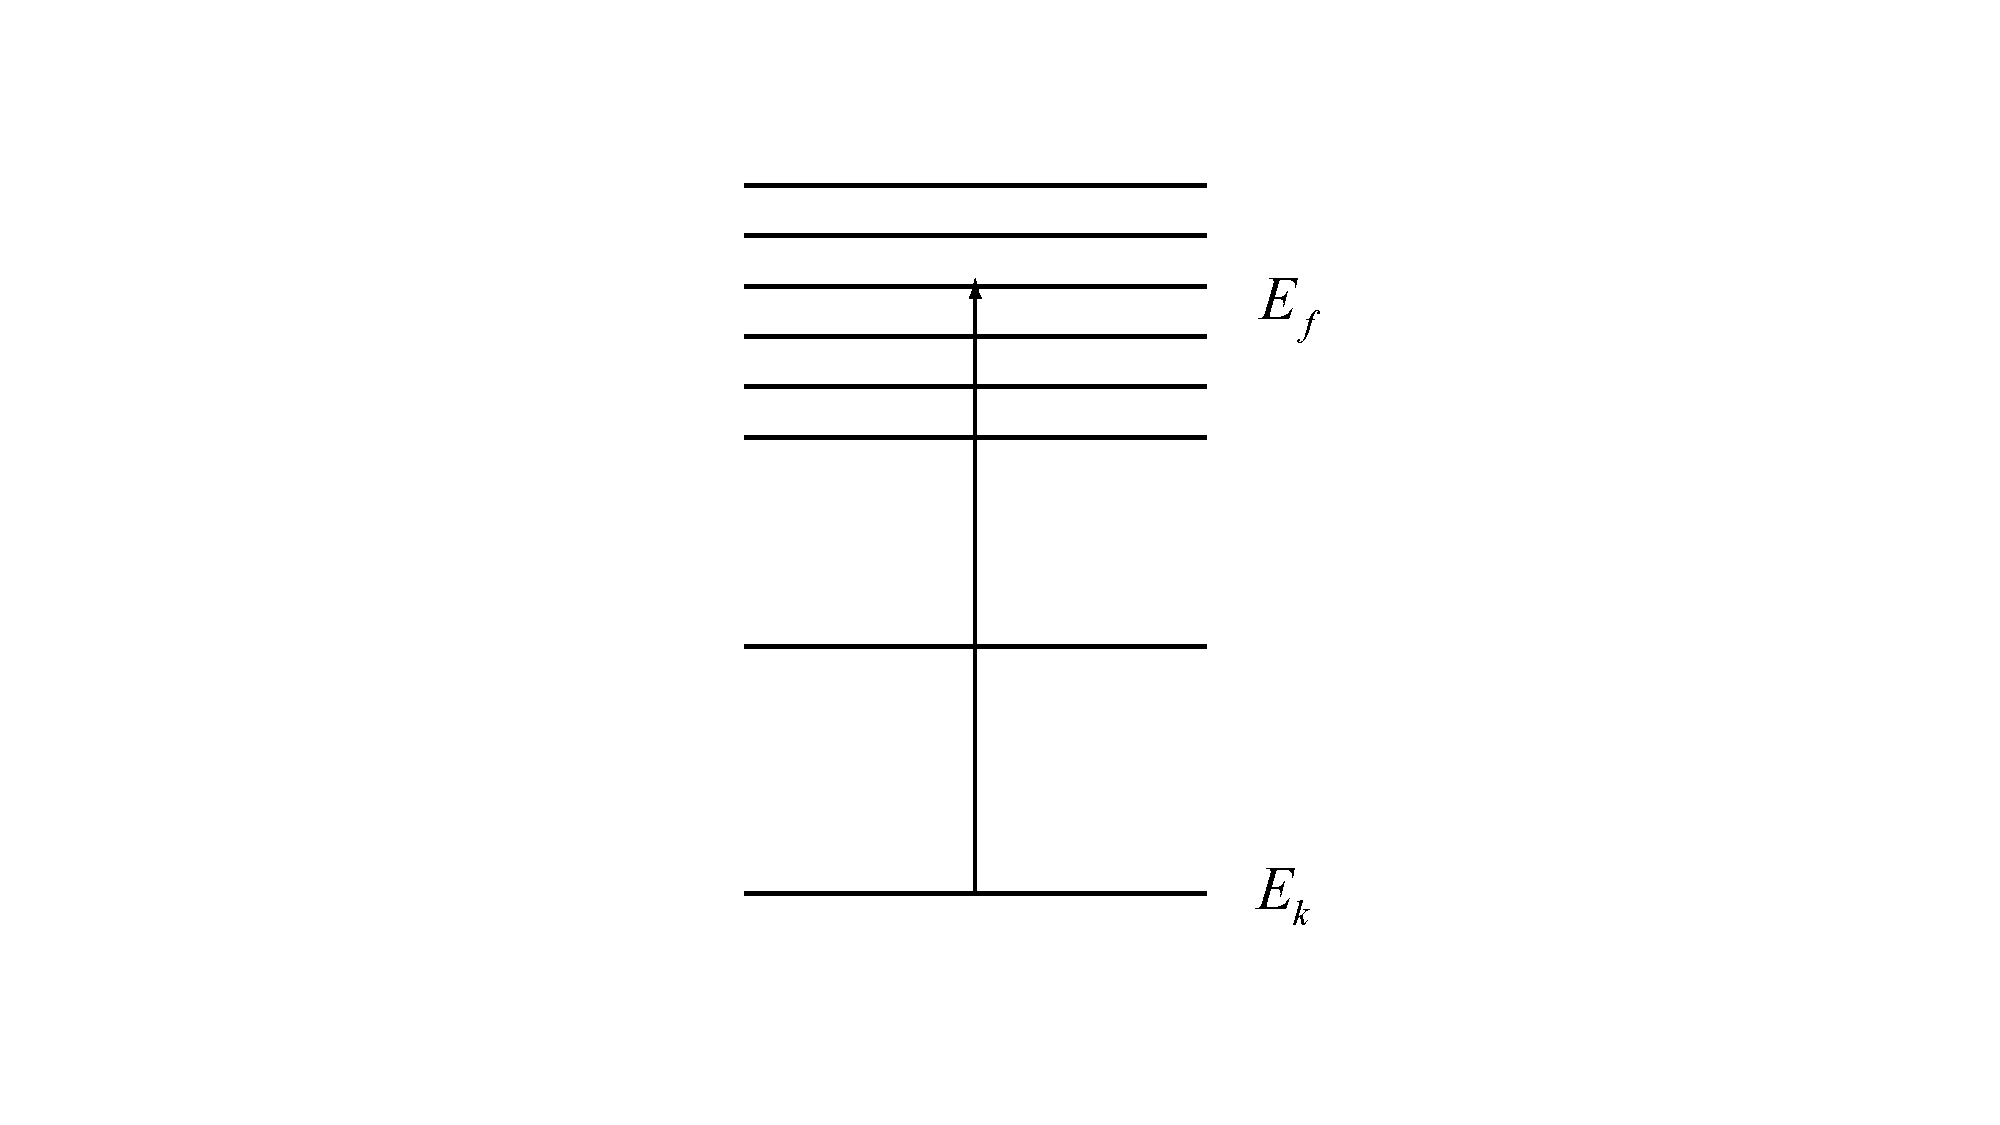
\includegraphics[width=3cm,clip]{QM file/figure/9-1}
	\caption{}\label{fig.9-1}
\end{wrapfigure}

仍设$H^{\prime}$为单频并取\eqref{eq92.1}式之形式.

连续能谱可以认为是能级密集的极限情形,如图\ref{fig.9-1}所示.由于终态能级密集,严格区分终态能量的微小差别既无可能,也无必要.有实际意义的做法是计算从初态$\varPsi_{k}$跃迁到能量接近$(E_{k}+\hbar\omega_{0})$的各个终态的概率总和.设在$E_{f}\approx(E_{k}+\hbar\omega_{0})$附近,能量范围$dE_{f}$内状态数为$\rho(E_{f})dE_{f}$,$\rho(E_{f})$称为状态密度.则由初态$\varPsi_{k}$向这些终态的跃迁速率总和为
\eqlong
\begin{equation}\label{eq92.11}
	W_{k\rightarrow f}=\int w_{k\rightarrow f}\rho(E_{f})dE_{f}
\end{equation}
将\eqref{eq92.9}式代入上式,得到
\begin{empheq}{equation}\label{eq92.12}
	\boxed{	W_{k\rightarrow f}=\frac{2\pi}{\hbar}|F_{fk}|^{2}\rho(E_{f}),\quad E_{f}=E_{k}+\hbar\omega_{0}	}
\end{empheq}\eqnormal
这公式有时称为黄金规则.在以上推导中假定$dE_{f}$范围内各个终态除能量略有差别外,其他方面的性质相同,特别是$F_{fk}$相同,这样由\eqref{eq92.11}式就得到\eqref{eq92.12}式.如果这些终态的$F_{fk}$有几种取值,则应按$F_{fk}$的数值将终态分类,对各类终态分别计算其状态密度和跃迁速率.

用紫外线(角频率$\omega_{0}$)照射原子,使原子中电子$(E_{k}<0)$电离$(E_{f}>0)$的过程(光电效应)就是属于本节讨论的问题.

{\heiti 3.常微扰}

设$t>0$时$H^{\prime}=H^{\prime}(x)$,与$t$无关这种情况相当于$\omega_{0}\rightarrow0$,只需在以上各公式中将$F_{fk}$换成$H_{fk}^{\prime}$,并取$\omega_{0}=0$就行了.例如\eqref{eq92.9}式改为
\begin{empheq}{equation}\label{eq92.13}
	w_{k\rightarrow f}\approx\frac{2\pi}{\hbar}|H_{fk}^{\prime}|^{2}\delta(E_{f}-E_{k})
\end{empheq}
其中$\delta$函数表明跃迁只能在能量相同的状态间发生.对于分立能级,常微扰将引起各简并态相互跃迁,结果导致这些简并态重新组合,形成新的定态.但如有某个简并态$\varPsi_{k}$,它与其他所有简并态(各$\varPsi_{f}$)之间$H_{fk}^{\prime}$均等于0,则$\varPsi_{k}$将不受微扰$H^{\prime}$的影响而保待其独立性,即在$H=H_{0}+H^{\prime}$的情况下,$\varPsi_{k}$仍是正确的定态波函数(在零级近似程度上,参看$\S$\ref{sec:06.02}).

\pskip
\example 弹性散射

按照量子跃迁的观点处理弹性散射,可以很便捷地导出散射截面的玻恩近似公式,如下.

\begin{figure}[!h]
	\centering
	\small
	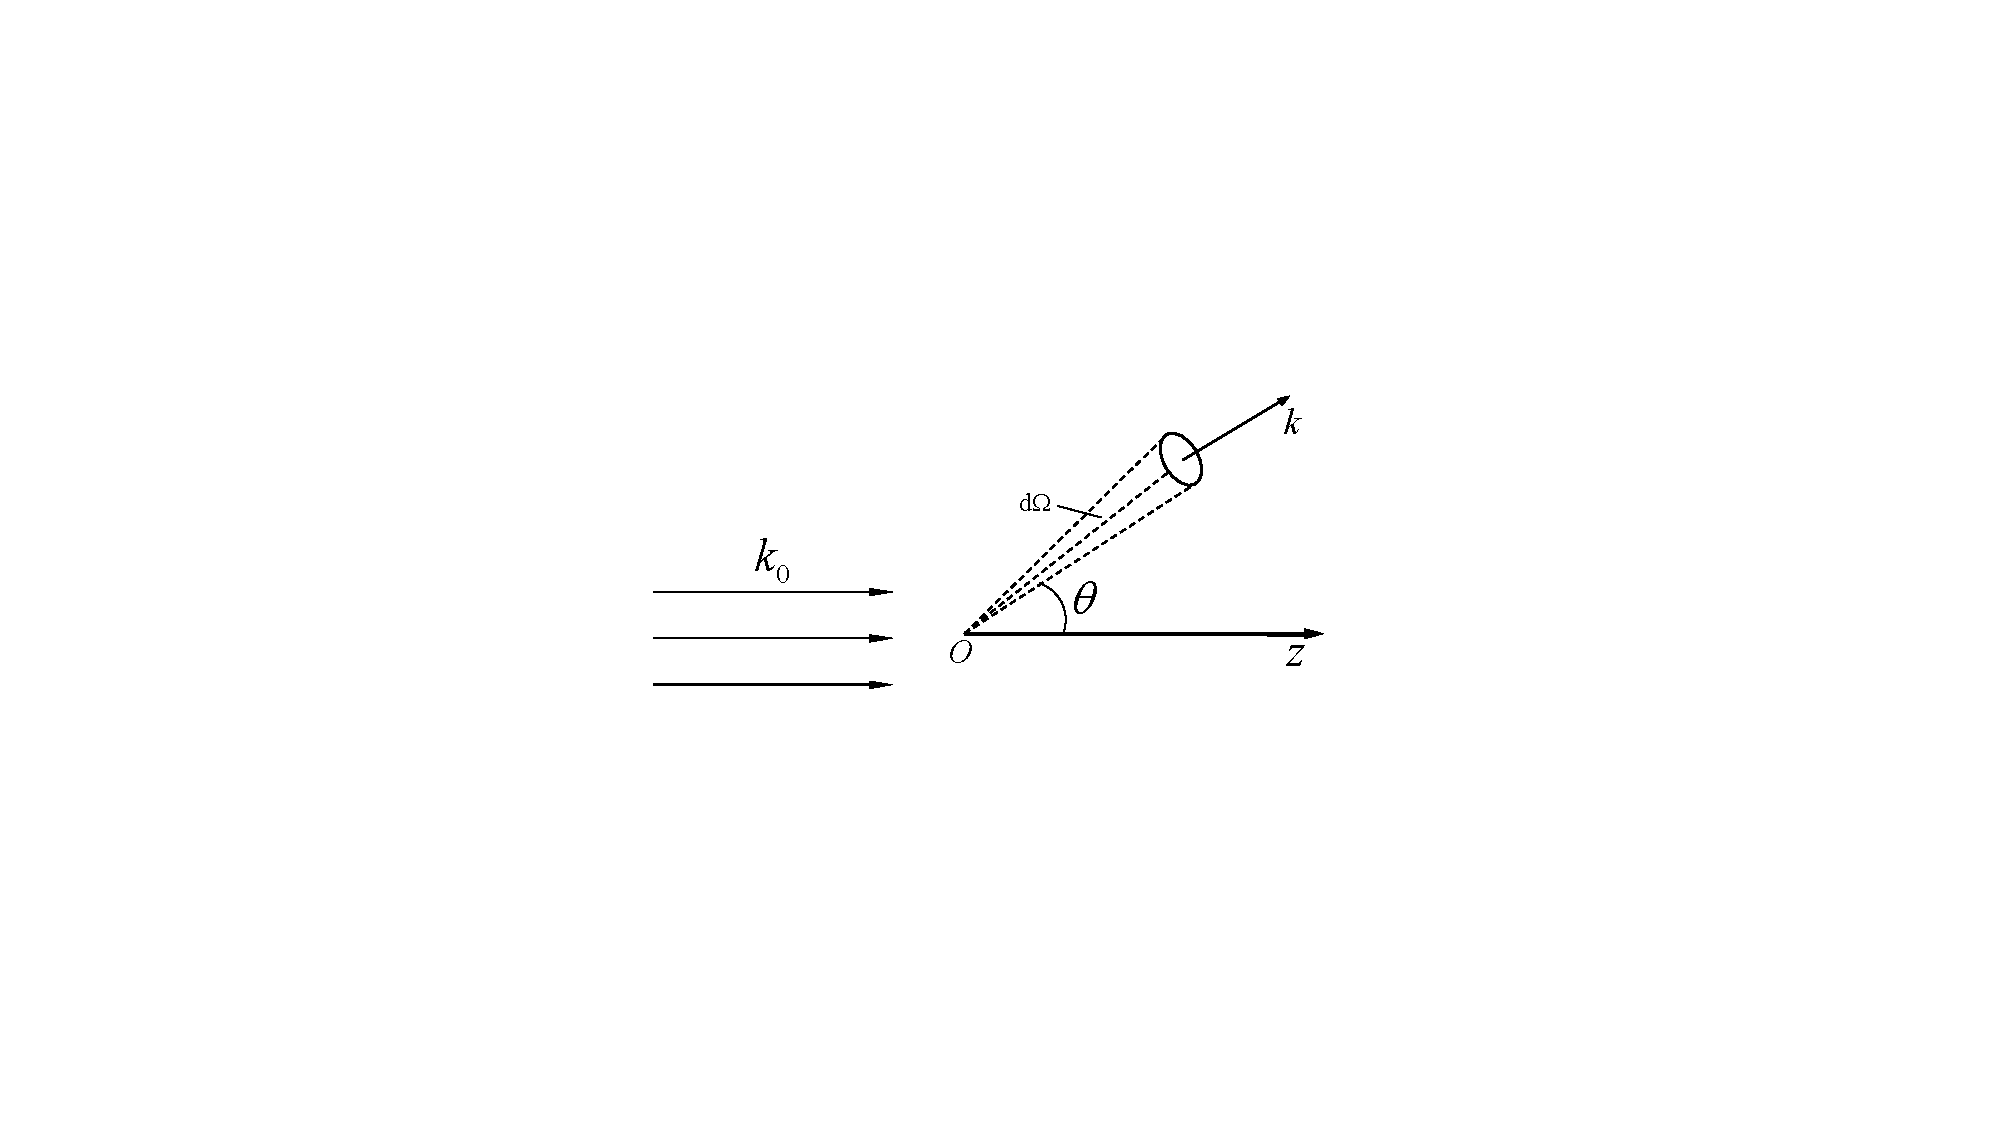
\includegraphics[width=6cm,clip]{QM file/figure/9-2}
	\caption{}\label{fig.9-2}
\end{figure}

散射过程中粒子的动量变化如图\ref{fig.9-2}所示.入射动量$\hbar k_{0}$,出射动量$\hbar k$,散射角$\theta$.为了便于计算状态密度,采用“箱归一化”方法($\S$\ref{sec:03.05}),“箱子”体积$L^{3}$.归一化的初态和终态波函数为
\begin{empheq}{align}
	\varPsi_{k_{0}}(\boldsymbol{r})=&L^{-\frac{3}{2}}e^{ik_{0}z}=L^{-\frac{3}{2}}e^{i\boldsymbol{k}_{0}\cdot\boldsymbol{r}}	\label{eq92.14}\\
	&\varPsi_{k}(\boldsymbol{r})=L^{-\frac{3}{2}}e^{i\boldsymbol{k}\cdot\boldsymbol{r}}	\label{eq92.15}
\end{empheq}
散射作用势视为常微扰,即令
\eqshort
\begin{empheq}{equation}\label{eq92.16}
	H^{\prime}=V(\boldsymbol{r})
\end{empheq}\eqnormal
在$V(\boldsymbol{r})$作用下粒子被散射到$(\theta,\varphi)$方向,相当于从初态$\varPsi_{k_{0}}$跃迁到终态$\varPsi_{k}$,由于终态动量$\hbar k$可以连续变化,应按连续谱处理,终态动量方向在$(\theta,\varphi)$附近$d\Omega$范围内的状态数为[参看\eqref{eq35.34}式]
\begin{empheq}{equation}\label{eq92.17}
	\rho(E)dE=\frac{L^{3}d^{3}\boldsymbol{p}}{h^{3}}=\frac{L^{3}\boldsymbol{p}^{2}dpd\Omega}{h^{3}}
\end{empheq}
终态动量与能量间有关系
\begin{empheq}{equation}\label{eq92.18}
	E=\frac{p^{2}}{2\mu},\quad dE=\frac{pdp}{\mu}
\end{empheq}
代入\eqref{eq92.17}式,即得
\begin{empheq}{equation}\label{eq92.19}
	\rho(E)=\frac{L^{3}\mu pd\Omega}{h^{3}}
\end{empheq}

由初态$\varPsi_{k_{0}}$跃迁到终态动量方向在$d\Omega$范围内的一切终态,跃迁速率总和可以按\eqref{eq92.12}式计算,即
\eqlong
\begin{empheq}{equation}\label{eq92.20}
	W=\frac{2\pi}{\hbar}|V_{kk_{0}}|^{2}\rho(E)=\frac{2\pi}{\hbar h^{3}}L^{3}\mu pd\omega|V_{kk_{0}}|^{2}
\end{empheq}\eqnormal
其中
\begin{empheq}{align}\label{eq92.21}
	V_{kk_{0}} &=\langle \varPsi_{k}|V|\varPsi_{k_{0}} \rangle 	\nonumber\\
	&=L^{-3}\int V(\boldsymbol{r})\exp[i(\boldsymbol{k_{0}}-\boldsymbol{k})\cdot\boldsymbol{r}]d^{3}\boldsymbol{r}
\end{empheq}

本题采用的“箱归一化”方法相当于体积$L^{3}$内有一个入射粒子,入射粒子流量为
\begin{empheq}{equation}\label{eq92.22}
	N_{0}=\frac{v}{L^{3}}=\frac{p}{\mu L^{3}}
\end{empheq}

单位时间内散射到$d\Omega$方向的粒子数$dN$应该就是由\eqref{eq92.20}式表示的跃迁速率和,即
\begin{empheq}{equation}\label{eq92.23}
	W=dN=N_{0}\sigma(\theta,\varphi)d\Omega
\end{empheq}
比较\eqref{eq92.20}、\eqref{eq92.22}、\eqref{eq92.23}式,即得微分散射截面公式.
\eqlong
\begin{empheq}{equation}\label{eq92.24}
	\sigma(\theta,\varphi)=\frac{\mu^{2}}{4\pi^{2}\hbar^{4}}\left|\int V(\boldsymbol{r})\exp[i(\boldsymbol{k_{0}}-\boldsymbol{k})\cdot\boldsymbol{r}]d^{3}\boldsymbol{r}\right|^{2}
\end{empheq}\eqnormal
这正是\eqref{eq84.32}式.$\S$\ref{sec:08.04}中$V(\boldsymbol{k},\boldsymbol{k_{0}})$相当于本题\eqref{eq92.21}式定义的$V_{kk_{0}}$乘以$L^{3}$.

如散射作用势$V$是中心力场,$V=V(r)$,则\eqref{eq92.21}中积分可以采用球坐标系,并以$(\boldsymbol{k_{0}}-\boldsymbol{k})$方向作为积分时的极轴,即令
\eqllong
\begin{empheq}{align*}
	&q=|\boldsymbol{k_{0}}-\boldsymbol{k}|,\quad (\boldsymbol{k_{0}}-\boldsymbol{k})\cdot\boldsymbol{r}=qr\cos\theta^{\prime}	\\
	\int V(r)\exp&[i(\boldsymbol{k_{0}}-\boldsymbol{k})\cdot\boldsymbol{r}]d^{3}\boldsymbol{r}=\int V(r)e^{iqr\cos\theta^{\prime}}r^{2}dr\sin\theta^{\prime}d\theta^{\prime}d\varphi^{\prime}
\end{empheq}\eqlong
其中角部积分可以算出,
\begin{empheq}{align}\label{eq92.25}
	\int e^{iqr\cos\theta^{\prime}}\sin\theta^{\prime}d\theta^{\prime}d\varphi^{\prime} &=2\pi\int_{0}^{\pi}e^{iqr\cos\theta^{\prime}}\sin\theta^{\prime}d\theta^{\prime}	\nonumber\\
	&=2\pi\int_{-1}^{1}e^{iqr\eta}d\eta=4\pi\frac{\sin qr}{qr}
\end{empheq}
因此
\begin{empheq}{equation}\label{eq92.26}
	\int V(r)\exp[i(\boldsymbol{k_{0}}-\boldsymbol{k})\cdot\boldsymbol{r}]d^{3}\boldsymbol{r}=\frac{4\pi}{q}\int_{0}^{\infty}\sin qrV(r)rdr
\end{empheq}\eqnormal
再代入\eqref{eq92.24}式,可求出$\sigma(\theta)$.\eqref{eq92.26}式中$q$是散射角$\theta$的函数,由图\ref{fig.9-2}可知
\begin{empheq}{equation}\label{eq92.27}
	q=|\boldsymbol{k_{0}}-\boldsymbol{k}|=2k\sin\left(\frac{\theta}{2}\right)
\end{empheq}




% 光的吸收与受激辐射
\section[光的吸收与受激辐射]{光的吸收与受激辐射} \label{sec:09.03} % 
% \makebox[5em][s]{} % 短题目拉间距

光被其他物质吸收与辐射的过程,就是光子的产生与湮没的过程.严格处理光的吸收与辐射问题,应该将电磁场作为量子力学体系,考虑它与其他物质(例如一个原子)的相互作用,以及由此而引起的双方的量子跃迁.这种理论属于量子电动力学范畴,超出初等量子力学课程的要求.本节将对问题作单方面的处理.以原子对光的吸收与辐射为物理模型,用量子跃迁理论来处理原子状态的变化问题,而电磁场的状态变化问题(即光子的产生与湮没过程)则不予考虑.亦即将着眼点放在原子上,而将光当作经典电磁波对待,它对原子产生作用,导致原子的状态发生变化.同时必须记得电磁波是量子化的,而且原子的能级跃迁过程符合能量守恒定律,当原子从$\varPsi_{k}$态跃迁到$\varPsi_{f}$态时,将同时吸收$(E_{k}<E_{f})$或放射$(E_{k}>E_{f})$一个光子$(\hbar\omega=|E_{f}-E_{k}|)$.

{\heiti 1. 原子的受激跃迁}

为简明起见,考虑一个单价原子价电子在原子核和内层电子的库仑场(等效成一个中心力场)中运动,如不考虑自旋-轨道耦合作用,其能量算符可以表示成
\begin{empheq}{equation}\label{eq93.1}
	H_{0}=-\frac{\hbar^{2}}{2m_{0}}\nabla^{2}+V(r)
\end{empheq}
能级记为$E_{nl}$,定态波函数($H_{0},\boldsymbol{L}^{2},L_{z}$共同本征函数)记为
\begin{empheq}{equation}\label{eq93.2}
	\varPsi_{nlm}(r,\theta,\varphi)=R_{nl}(r)Y_{lm}(\theta,\varphi)
\end{empheq}
(为了简明,暂不考虑自旋自由度.)
\noindent 光波的电、磁场$(\mathscr{E},\boldsymbol{B})$对价电子的作用势可以近似表示成
\eqshort
\begin{empheq}{equation*}
	H^{\prime}\approx-\mathscr{E}\cdot\boldsymbol{D}-\boldsymbol{B}\cdot\boldsymbol{\mu}
\end{empheq}
其中第一项是电场对电子电矩的作用,第二项是磁场对电子磁矩的作用.在高斯单位制中光波的$\mathscr{E}$与$\boldsymbol{B}$数值相等.价电子电矩与磁矩的量级约为
\begin{empheq}{align*}
	D&\sim ea_{0}=\frac{\hbar^{2}}{em_{e}}	\\
	\mu&\sim \mu_{B}=\frac{e\hbar}{2m_{e}c}
\end{empheq}\eqnormal
因此,$H^{\prime}$中电作用势与磁作用势的比值约为
\begin{empheq}{equation*}
	\frac{\boldsymbol{B}\cdot\boldsymbol{\mu}}{\mathscr{E}\cdot\boldsymbol{D}}\sim\frac{\mu}{D}\sim\frac{e^{2}}{2\hbar c}<\frac{1}{100}
\end{empheq}
通常可以略去磁作用势而取近似
\begin{empheq}{equation}\label{eq93.3}
	H^{\prime}\approx-\mathscr{E}\cdot\boldsymbol{D}=e\mathscr{E}\cdot\boldsymbol{r}
\end{empheq}
电场$\mathscr{E}$的函数形式视光波的性质而定,例如波矢量为$k$$\bigg($波长$\lambda=\frac{2\pi}{k}\bigg)$的线偏振光,光波电场为
\begin{empheq}{equation}\label{eq93.4}
	\mathscr{E}(\boldsymbol{r},t)=\mathscr{E}_{0}\cos(\boldsymbol{k}\cdot\boldsymbol{r}-\omega t)
\end{empheq}
能够引起原子能级跃迁的光波主要是可见光或紫外光,其波长入约为原子半径的几千倍,因此在原子范围内
\begin{empheq}{equation*}
	\boldsymbol{k}\cdot\boldsymbol{r}\sim\frac{2\pi a_{0}}{\lambda}\ll 1
\end{empheq}
可以忽略电场$\mathscr{E}$的空间变化,而取
\begin{empheq}{equation*}\label{eq93.4'}
	\mathscr{E}(t)\approx\mathscr{E}_{0}\cos\omega t=\boldsymbol{l}\mathscr{E}_{0}\cos\omega t
	\tag{$9.3.4^{\prime}$}
\end{empheq}
$\boldsymbol{l}$为电场的偏振方向单位矢量.代入\eqref{eq93.3}式,得到
\begin{empheq}{align}\label{eq93.5}
	H^{\prime} &=e\mathscr{E}_{0}\boldsymbol{l}\cdot\boldsymbol{r}\cos\omega t	\nonumber\\
	&=\frac{1}{2}e\mathscr{E}_{0}\boldsymbol{l}\cdot\boldsymbol{r}(e^{i\omega t}+e^{-i\omega t})
\end{empheq}
这正是$\S$\ref{sec:09.02}讨论过的单频微扰,相当于\eqref{eq92.1}式中
\begin{empheq}{equation}\label{eq93.6}
	\hat{F}=\frac{1}{2}e\mathscr{E}_{0}\boldsymbol{l}\cdot\boldsymbol{r}
\end{empheq}
在这光波照射下,价电子由初态$\varPsi_{nlm}\rightarrow$终态$\varPsi_{n^{\prime}l^{\prime}m^{\prime}}$的跃迁速率可以按照\eqref{eq92.9}式计算(和$\S$\ref{sec:09.02}一样,设$E_{n^{\prime}l^{\prime}}>E_{nl}$)
\eqllong
\begin{empheq}{equation}\label{eq93.7}
	w_{nlm\rightarrow n^{\prime}l^{\prime}m^{\prime}}=\frac{\pi}{2}\frac{e^{2}}{\mathscr{E}_{0}^{2}}|(\boldsymbol{l}\cdot\boldsymbol{r})_{n^{\prime}l^{\prime}m^{\prime},nlm}|^{2}\delta(E_{n^{\prime}l^{\prime}}-E_{nl}-\hbar\omega)
\end{empheq}\eqlong
其中$\delta$函数表明,只有$E_{n^{\prime}l^{\prime}}-E_{nl}\approx\hbar\omega$(光子能量),跃迁才有可能发生.由\eqref{eq93.4}式表示的光波,单位体积中光能为
\begin{empheq}{equation*}
	u=\frac{1}{8\pi}(\mathscr{E}^{2}+\boldsymbol{B}^{2})_{\text{时间平均}}=\frac{1}{4\pi}(\mathscr{E}^{2})_{\text{时间平均}}=\frac{1}{8\pi}\mathscr{E}_{0}^{2}
\end{empheq}\eqindent{1}
\eqref{eq93.7}式中$\mathscr{E}$用$u$来表示,得到
\begin{empheq}{equation*}\label{eq93.7'}
	w_{nlm\rightarrow n^{\prime}l^{\prime}m^{\prime}}=\frac{4\pi^{2}}{\hbar}ue^{2}|(\boldsymbol{l}\cdot\boldsymbol{r})_{n^{\prime}l^{\prime}m^{\prime},nlm}|^{2}\delta(E_{n^{\prime}l^{\prime}}-E_{nl}-\hbar\omega)	\tag{$9.3.7^{\prime}$}
\end{empheq}\eqshort
跃迁速率和光波能量密度$u$成正比,这是受激跃迁的特点.

实际的光波不可能是严格单频的,总是有频率分布的,设
\begin{empheq}{equation}\label{eq93.8}
	u=\int_{0}^{\infty}\rho(\omega)d\omega
\end{empheq}\eqnormal
$\rho(\omega)d\omega$是单位体积中频率范围$(\omega,\omega+d\omega)$内光波能量.将\eqref{eq93.8}式代入\eqref{eq93.7}式,计及$\delta$函数的积分效果
\begin{empheq}{equation*}
	\int_{0}^{\infty}\rho(\omega)\delta(E-\hbar\omega)d(\hbar\omega)=\rho\left(\frac{E}{\hbar}\right)
\end{empheq}\eqlong
可得
\begin{empheq}{equation}\label{eq93.9}
	w_{nlm\rightarrow n^{\prime}l^{\prime}m^{\prime}}=\frac{4\pi^{2}}{\hbar^{2}}\rho(\omega_{n^{\prime}l^{\prime},nl})e^{2}|(\boldsymbol{l}\cdot\boldsymbol{r})_{n^{\prime}l^{\prime}m^{\prime},nlm}|^{2}
\end{empheq}
其中
\eqshort
\begin{empheq}{equation*}
	(\omega_{n^{\prime}l^{\prime},nl})=\frac{E_{n^{\prime}l^{\prime}}-E_{nl}}{\hbar}
\end{empheq}\eqnormal
\eqref{eq93.9}式中的矩阵元应该作如下理解:设偏振矢量与$x,y,z$轴的夹角分别为$\alpha,\beta,\gamma$,则
\eqlong
\begin{empheq}{align}\label{eq93.10}
	\boldsymbol{l}\cdot\boldsymbol{r}&=x\cos\alpha+y\cos\beta+z\cos\gamma	\nonumber\\
	(\boldsymbol{l}\cdot\boldsymbol{r})_{n^{\prime}n}&=x_{n^{\prime}n}\cos\alpha+y_{n^{\prime}n}\cos\beta+z_{n^{\prime}n}\cos\gamma
\end{empheq}\eqllong
($n$代表$nlm$,$n^{\prime}$代表$n^{\prime}l^{\prime}m^{\prime}$,下同.)
\begin{empheq}{align*}
	|(\boldsymbol{l}\cdot\boldsymbol{r})_{n^{\prime}n}|^{2} &=(x_{n^{\prime}n})^{*}x_{n^{\prime}n}\cos^{2}\alpha+(y_{n^{\prime}n})^{*}y_{n^{\prime}n}\cos^{2}\beta+\cdots+	\\
	&[(x_{n^{\prime}n})^{*}y_{n^{\prime}n}+x_{n^{\prime}n}(y_{n^{\prime}n})^{*}]\cos\alpha\cos\beta+\cdots
\end{empheq}\eqnormal
如果光波的偏振方向是完全混乱的(例如热辐射场就是这样),则\eqref{eq93.9}式应该对$\boldsymbol{l}$的各种方向平均,这时
\eqlong
\begin{empheq}{align*}
	(\cos^{2}\alpha)_{\text{平均}}&=(\cos^{2}\beta)_{\text{平均}}=(\cos^{2}\gamma)_{\text{平均}}=\frac{1}{3}	\\
	&(\cos\alpha\cos\beta)_{\text{平均}}=0,\text{等等}
\end{empheq}
\begin{empheq}{align}\label{eq93.11}
	|(\boldsymbol{l}\cdot\boldsymbol{r})_{n^{\prime}n}|_{\text{平均}}^{2} &=\frac{1}{3}(|x_{n^{\prime}n}|^{2}+|y_{n^{\prime}n}|^{2}+|z_{n^{\prime}n}|^{2})	\nonumber\\
	\text{(定义)}&=\frac{1}{3}|\boldsymbol{r}_{n^{\prime}n}|^{2}
\end{empheq}
这样,当光波偏振完全混乱时,跃迁速率公式为
\begin{empheq}{align}\label{eq93.12}
	w_{nlm\rightarrow n^{\prime}l^{\prime}m^{\prime}}&=\frac{4\pi^{2}}{3\hbar^{2}}\rho(\omega_{n^{\prime}l^{\prime},nl})e^{2}|\boldsymbol{r}_{n^{\prime}l^{\prime}m^{\prime},nlm}|^{2}	\nonumber\\
	&=\frac{4\pi^{2}}{3\hbar^{2}}\rho(\omega_{n^{\prime}l^{\prime},nl})|\boldsymbol{D}_{n^{\prime}l^{\prime}m^{\prime},nlm}|^{2}
\end{empheq}\eqshort
跃迁速率与电偶极矩$(\boldsymbol{D}=-e\boldsymbol{r})$矩阵元有关,故上式又称受激电偶极跃迁速率.

受激跃迁最本质性的规律是跃迁速率$w$和光能频率分布密度$\rho$成正比\eqref{eq93.9}式及\eqref{eq93.12}式清楚地表明$nlm$态与$n^{\prime}l^{\prime}m^{\prime}$态间的跃迁是入射光中频率为$\omega_{n^{\prime}l^{\prime},nl}$的成分引起的,如入射光中没有这种频率成分,跃迁就不会发生.当跃迁$\varPsi_{nlm}\rightarrow\varPsi_{n^{\prime}l^{\prime}m^{\prime}}$发生时,原子将从光波吸收能量$(E_{n^{\prime}l^{\prime}}-E_{nl})$,即吸收一个能量为$\hbar\omega_{n^{\prime}l^{\prime},nl}$的光子.根据$\S$\ref{sec:09.01}的分析,同样的入射光也能引起反方向的跃迁,即$\varPsi_{n^{\prime}l^{\prime}m^{\prime}}\rightarrow\varPsi_{nlm}$,而且
\begin{empheq}{equation}\label{eq93.13}
	w_{n^{\prime}l^{\prime}m^{\prime}\rightarrow nlm}=w_{nlm\rightarrow n^{\prime}l^{\prime}m^{\prime}}
\end{empheq}
当跃迁$\varPsi_{n^{\prime}l^{\prime}m^{\prime}}\rightarrow\varPsi_{nlm}$发生时,原子由高能级跳到低能级,同时放出一个频率为$\omega_{n^{\prime}l^{\prime},nl}$的光子.

从光的吸收与辐射角度看问题,原子从$\varPsi_{k}$态向$\varPsi_{f}$态的跃迁速率可以写成
\begin{empheq}{equation}\label{eq93.14}
	w_{k\rightarrow f}=B_{kf}\rho(\omega_{fk})
\end{empheq}
$B_{kf}$称为吸收系数.$(E_{k}<E_{f})$相反方向$(\varPsi_{f}\rightarrow\varPsi_{k})$的跃迁速率可以写成
\begin{empheq}{equation*}\label{eq93.14'}
	w_{f\rightarrow k}=B_{fk}\rho(\omega_{fk})
	\tag{$9.3.14^{\prime}$}
\end{empheq}\eqnormal
$B_{kf}$称为受激辐射系数.由于$w_{k\rightarrow f}=w_{f\rightarrow k}$,所以$B_{kf}=D_{fk}$.在入射光偏振混乱的条件下,由\eqref{eq93.12}式可知
\begin{empheq}{equation}\label{eq93.15}
	B_{kf}=B_{fk}=\frac{4\pi^{2}}{3\hbar^{2}}e^{2}|\boldsymbol{r}_{fk}|^{2}
\end{empheq}
注意,$B$系数完全由原子初、终态的性质决定,和入射光强度无关.

{\heiti 2. 选择定则}

原子在光波照射下发生受激跃迁,必须矩阵元\eqref{eq93.10}式不等于零才行.与此相应,初、终态量子数及宇称性的变化将受到某些限制,称为选择定则.

根据球谐函数$Y_{lm}$的递推公式[附录\ref{A04}\eqref{eqA4.45}、\eqref{eqA4.46}式]及正交性,易得下列选择定则:
\eqlong
\begin{empheq}{align}\label{eq93.16}
	&z_{n^{\prime}l^{\prime}m^{\prime},nlm}\neq0,\longrightarrow l^{\prime}=l\pm1,m^{\prime}=m	\nonumber\\
	&(x+iy)_{n^{\prime}l^{\prime}m^{\prime},nlm}\neq0,\longrightarrow l^{\prime}=l\pm1,m^{\prime}=m+1	\nonumber\\
	&(x-iy)_{n^{\prime}l^{\prime}m^{\prime},nlm}\neq0,\longrightarrow l^{\prime}=l\pm1,m^{\prime}=m-1	\\
	&\begin{rcases}
		x_{n^{\prime}l^{\prime}m^{\prime},nlm}\neq0 \nonumber\\
		y_{n^{\prime}l^{\prime}m^{\prime},nlm}\neq0	\nonumber
	\end{rcases}\longrightarrow l^{\prime}=l\pm1,m^{\prime}=m\pm1	\nonumber
\end{empheq}\eqnormal
$\varPsi_{nlm}$的宇称为$(-1)^{l}$,$\varPsi_{n^{\prime}l^{\prime}m^{\prime}}$的宇称为$(-1)^{l^{\prime}}$,$\boldsymbol{r}$的宇称为负,所以电偶极跃迁的宇称选择定则为$(l^{\prime}-l)=\pm1$,即初、终态宇称相反.

入射光偏振混乱时,为了跃迁$\varPsi_{nlm}\rightarrow\varPsi_{n^{\prime}l^{\prime}m^{\prime}}$成为可能,只需$\boldsymbol{r}$的任何一个分量$(x,y,z)$的矩阵元不为0,所以选择定则是
\eqlong
\begin{empheq}{equation}\label{eq93.17}
	\Delta l=l^{\prime}-l=\pm1,\quad \Delta m=m^{\prime}-m=0,\pm1
\end{empheq}
如入射光有特殊偏振性质,选择定则应根据作用势$H^{\prime}$的具体结构来确定.

如考虑电子的自旋自由度,计及自旋-轨道耦合能,价电子状态由量子数$nljm_{j}$表示(见$\S$\ref{sec:07.03}).但对于受激电偶极跃迁,光波对价电子的作用势仍由\eqref{eq93.5}式表示,所以跃迁速率公式只需将\eqref{eq93.9}或\eqref{eq93.12}式中量子数作相应替换($nlm\rightarrow nljm_{j}$,等等)就行.可以证明\footnote{参阅:钱伯初,曾谨言$\cdot$量子力学习题精选与剖析$\cdot$上册第2版$\cdot$北京:科学出版社,1999.10.7题}$\boldsymbol{r}_{n^{\prime\cdots,n\cdots}}$的选择定则(即电偶极跃迁选择定则)是
\begin{empheq}{equation}\label{eq93.18}
	j^{\prime}-j=0,\pm1,\quad l^{\prime}-l=\pm1,\quad m_{j}^{\prime}-m_{j}=0,\pm1
\end{empheq}\eqnormal
径向量子数$(n,n^{\prime})$的变化不受限制,没有选择定则.

\pskip
\example 用沿正$z$轴方向传播的右旋圆偏振光(频率$\omega$)照射单价原子,造成价电子的受激跃迁,设价电子原来处于$\varPsi_{nlm}$态,求跃迁选择定则.

\solution 右旋偏振光波电场$\mathscr{E}$的旋转方向符合右手螺旋法则,如在原子范围内略去电场的空间变化,$\mathscr{E}(t)$可以表示成
\begin{empheq}{equation}\label{eq93.19}
	\mathscr{E}_{x}=\mathscr{E}_{0}\cos\omega t,\quad \mathscr{E}_{y}=\mathscr{E}_{0}\sin\omega t,\quad \mathscr{E}_{z}=0
\end{empheq}
光波对价电子的作用势(电偶极近似)为
\begin{empheq}{align}\label{eq93.20}
	H^{\prime}&=e\mathscr{E}\cdot\boldsymbol{r}=e\mathscr{E}_{0}(x\cos\omega t+y\sin\omega t)	\nonumber\\
	&=(x-iy)e\mathscr{E}_{0}e^{i\omega t}+(x+iy)e\mathscr{E}_{0}e^{i\omega t}
\end{empheq}
设价电子的能态跃迁为$\varPsi_{nlm}\rightarrow\varPsi_{n^{\prime}l^{\prime}m^{\prime}}$,分两种情形讨论:
\begin{subequations}
	(a) $E_{nl}<E_{n^{\prime}l^{\prime}}$,电子跃迁时吸收光子.\eqref{eq93.20}式中$e^{i\omega t}$项对跃迁造成贡献(当$E_{n^{\prime}l^{\prime}}-E_{nl}\approx\hbar\omega$),跃迁矩阵元为$(x+iy)_{n^{\prime}l^{\prime}m^{\prime},nlm}$,由\eqref{eq93.16}式可知选择定则为
	\begin{empheq}{equation}\label{eq93.21a}
		l^{\prime}-l=\pm1,\quad m^{\prime}-m=1
	\end{empheq}
	
	(b) $E_{nl}>E_{n^{\prime}l^{\prime}}$,电子跃迁时放射光子.\eqref{eq93.20}式中$e^{i\omega t}$项对跃迁产生贡献,跃迁矩阵元为$(x-iy)_{n^{\prime}l^{\prime}m^{\prime},nlm}$,选择定则为
	\begin{empheq}{equation}\label{eq93.21b}
		l^{\prime}-l=\pm1,\quad m^{\prime}-m=-1
	\end{empheq}
\end{subequations}
以上结果可以用角动量守恒定律解释如下.光子自旋为$\hbar$,其$z$分量为$\hbar,0,-\hbar$.本题涉及的右旋偏振光,$S_{z}=\hbar$.如电子吸收一个光子,电子角动量的$z$分量$(L_{z})$将增加$\hbar$,所以$m^{\prime}-m=1$;如电子放射一个光子,$L_{z}$将减少$\hbar$,所以$m^{\prime}-m=-1$.量子数$l$的选择定则$\Delta l=\pm1$也可以用电子-光子角动量耦合的三角形法则结合宇称法则(电偶极矩是奇宇称,所以初、终态宇称要变)而得到解释.




% 自发辐射
\section[自发辐射]{自发辐射} \label{sec:09.04} % 
% \makebox[5em][s]{} % 短题目拉间距

实验发现,当原子处于激发态时,即使没有外来的光波照射,原子也能自发地跃迁到较低能级,同时辐射出一个光子.这种过程称为自发跃迁或自发辐射.事实上,在几千度的温度下,原子发光主要来自自发辐射.原子核的自发跃迁则产生$\gamma$射线.

按照量子力学原理,如果没有外界作用,孤立体系将永远处于原来的定态能级,不应发生能级跃迁.那么,造成原子自发跃迁的原因是什么呢?原因是电磁场“真空” (光子数为0)的“零点振动”对于原子的作用.自发跃迁的严格理论属于量子电动力学范围.本节向读者介绍爱因斯坦在1917年建立的半唯象理论,当时量子力学尚未产生,爱因斯坦在玻尔量子论的基础上,将原子对光的吸收与辐射问题与统计物理原理巧妙地结合起来考虑,建立了自发跃迁与受激跃迁的关系.

考虑许多构造相同的原子和电磁辐射场达到热平衡.考虑原子的任何两个能级$E_{f}>E_{k}$,设处于能量本征态$\varPsi_{k}$与$\varPsi_{f}$的原子数分别为$N_{k}$与$N_{f}$.辐射场能量密度的频率分布表示成
\begin{empheq}{equation}\label{eq94.1}
	u=\int_{0}^{\infty}\rho(\omega)d\omega
\end{empheq}
爱因斯坦认为,单位时间内发生受激跃迁$\varPsi_{k}\rightarrow\varPsi_{f}$的原子数应该与$\rho(\omega_{fk})$成正比,自发跃迁则与光能密度无关而由原子自身的性质决定.当然,跃迁过程必须服从能量守恒定律,因此自发跃迁只能由高能量状态变到低能量状态,同时放出一个光子.设$\Delta t$时间内由$\varPsi_{k}$态跃迁到$\varPsi_{f}$态的原子数为
\begin{empheq}{equation}\label{eq94.2}
	\Delta N_{k\rightarrow f}=N_{k}B_{kf}\rho(\omega_{fk})\Delta t
\end{empheq}
$B_{kf}$称为原子的吸收系数.$\Delta t$时间内由$\varPsi_{f}$态跃迁到$\varPsi_{k}$态的原子数设为
\begin{empheq}{equation}\label{eq94.3}
	\Delta N_{f\rightarrow k}=N_{f}[A_{fk}+B_{fk}\rho(\omega_{fk})]\Delta t
\end{empheq}
$B_{fk}$是原子的受激辐射系数,$A_{fk}$是自发辐射系数(即自发跃迁速率).在热平衡时,正反两种跃迁的原子数变化应该相等,以维持各能态的原子数不变(细致平衡原理),即$\Delta N_{k\rightarrow f}=\Delta N_{f\rightarrow k}$.由此得到关系
\begin{empheq}{equation}\label{eq94.4}
	N_{f}[A_{fk}+B_{fk}\rho(\omega_{fk})]=N_{k}B_{kf}\rho(\omega_{fk})
\end{empheq}
上式中,$N_{f}$,$N_{k}$及$\rho(\omega_{fk})$都是温度$T$的函数.而$A$系数及$B$系数则是单个原子的性质,与温度无关.按照统计物理中的玻尔兹曼分布律,热平衡时各能态的原子数分布规律是
\begin{empheq}{equation}\label{eq94.5}
	\frac{N_{k}}{N_{f}}=\exp\left(\frac{E_{f}-E_{k}}{kT}\right)=\exp\left(\frac{\hbar\omega_{fk}}{kT}\right)
\end{empheq}
当$T\rightarrow\infty$,$N_{f}$与$N_{k}$趋于相等,而辐射场能量密度$u\propto T_{4}\rightarrow\infty$,同时$\rho(\omega)\propto kT\rightarrow\infty$.这时由\eqref{eq94.4}式可见$B_{kf}=B_{fk}$.于是\eqref{eq94.4}式可以化成
\begin{empheq}{equation*}\label{eq94.4'}
	\rho(\omega)=\frac{A_{fk}/B_{fk}}{N_{k}/N_{f}-1}=\frac{A_{fk}/B_{fk}}{e^{\hbar\omega/kT}-1}\quad (\omega=\omega_{fk})
	\tag{$9.4.4^{\prime}$}
\end{empheq}
就$\rho(\omega)$与温度$T$的函数关系而言,上式正是黑体辐射普朗克公式的基本形式,所以爱因斯坦关于辐射的唯象理论也是推导普朗克公式的一种方法.

再考虑\eqref{eq94.4'}式的高温极限.当$kT\gg\hbar\omega$,每一种电磁场振动模式具有的能量趋于$kT$,$\rho(\omega)$表现成瑞利-金斯公式
\begin{empheq}{equation}\label{eq94.6}
	\rho(\omega)=\frac{\omega^{2}kT}{\pi^{2}c^{3}}\quad (kT\gg\hbar\omega)
\end{empheq}
代入\eqref{eq94.4'}式,并取$e^{\hbar\omega/kT}-1\approx\frac{\hbar\omega}{kT}$,即可得到
\begin{empheq}{equation}\label{eq94.7}
	\frac{A_{fk}}{B_{fk}}=\frac{\hbar\omega_{fk}^{3}}{\pi^{2}c^{3}}
\end{empheq}
将这关系代入\eqref{eq94.4'}式,可得
\begin{empheq}{equation}\label{eq94.8}
	\rho(\omega)=\frac{\hbar\omega^{3}}{\pi^{2}c^{3}}bigg\ (e^{\hbar\omega/kT}-1)
\end{empheq}
这正是普朗克公式.以上是爱因斯坦半唯象辐射理论的基本内容.

将\eqref{eq94.7}式与\eqref{eq93.15}式联系起来,就可得到原子自发辐射系数(自发跃迁速率)的公式
\begin{empheq}{equation}\label{eq94.9}
	\boxed{ A_{fk}=\frac{4\omega_{fk}^{3}}{3\hbar c^{3}}e^{2}|\boldsymbol{r}_{fk}|^{2}	}
\end{empheq}
量子电动力学也给出同样的结果.如以光子能量$\hbar\omega_{fk}$乘上式,就得到原子的自发辐射功率:
\begin{empheq}{equation}\label{eq94.10}
	P_{fk}=\hbar\omega_{fk}A_{fk}=\frac{4\omega_{fk}^{3}}{3c^{3}}|\boldsymbol{D}_{fk}|^{2}
\end{empheq}
上式形式上不含$\hbar$,并和经典电动力学中电偶极矩振子的辐射功率公式相似,$2\boldsymbol{D}_{fk}$相当于经典电偶极矩振幅.一般地,由量子力学导出的不含$\hbar$的公式,都可给予经典物理的解释.

原子的受激跃迁速率($\S$\ref{sec:09.03})为
\begin{empheq}{equation}\label{eq94.11}
	w_{f\rightarrow k}=B_{fk}\rho(\omega_{fk})
\end{empheq}
联系\eqref{eq94.7}、\eqref{eq94.8}式,得到受激跃迁速率与自发跃迁速率的关系:
\begin{empheq}{equation}\label{eq94.12}
	w_{f\rightarrow k}=\frac{A_{fk}}{e^{\hbar\omega/kT}-1},\quad \omega=\omega_{fk}
\end{empheq}
热平衡时,频率为$\omega$的每种光子态的光子数密度为
\begin{empheq}{equation}\label{eq94.13}
	n(\omega)=\frac{1}{e^{\hbar\omega/kT}-1}
\end{empheq}
所以\eqref{eq94.12}式亦即
\begin{empheq}{equation*}\label{eq94.12'}
	w_{f\rightarrow k}=A_{fk}n(\omega_{fk})
	\tag{$9.4.12^{\prime}$}
\end{empheq}
此式反映出受激跃迁与自发跃迁的实质性联系.数值计算表明,当$\frac{\hbar\omega_{fk}}{kT}>\num{0.6931},n(\omega_{fk})<1,w_{f\rightarrow k}<A_{fk}$;当$\frac{\hbar\omega_{fk}}{kT}<\num{0.6931},n(\omega_{fk})>1,w_{f\rightarrow k}>A_{fk}$.例如$\omega_{fk}$属于可见光,如波长$\lambda\sim\num{600}\si{nm}$,必须$T>\num{3.46}\times10^{4}\si{K}$,受激跃迁速率才能超过自发跃迁速率.对于温度是几千度的原子气体,辐射的可见光主要来自自发辐射.

自发跃迁的选择定则由$\boldsymbol{r}_{fk}\neq0$决定,具体结果见\eqref{eq93.17}式,对于原子的电偶极跃迁,选择定则为$\Delta l=\pm1,\Delta m=0,\pm1$.

应该指出,\eqref{eq94.9}式并不是自发跃迁速率的严格结果,因为导出\eqref{eq94.9}式时利用了\eqref{eq94.7}式和\eqref{eq93.15}式,\eqref{eq94.7}式是严格的,而\eqref{eq93.15}式是对光波与原子的相互作用取电偶极近似后得到的结果,其特点是跃迁速率比例于原子电偶极矩$(\boldsymbol{D}=-e\boldsymbol{r})$矩阵元$(\boldsymbol{D}_{fk})$的绝对值平方.所以当自发跃迁$\varPsi_{n^{\prime}l^{\prime}m^{\prime}}\rightarrow\varPsi_{nlm}$不符合电偶极跃迁选择定则时,跃迁仍有可能通过光波与原子间的磁偶极矩作用或电四极矩作用而实现,但跃迁速率约为正常的电偶极跃迁速率的$\left(\frac{e^{2}}{\hbar c}\right)\sim10^{-4}$倍.如果$\varPsi_{n^{\prime}l^{\prime}m^{\prime}}$态和$\varPsi_{nlm}$态间一切电磁多极矩作用引起的跃迁均被选择定则禁止,则这两个状态间直接电磁跃迁就是严格禁止的.从s态$(l=0)$到s态的跃迁就属于这种严格禁止的情形.

\pskip
\example 计算氢原子2p$\rightarrow$1s自发跃迁速率和2p态平均寿命(不考虑自旋).

\solution 1s态即基态$\varPsi_{100}$,2p态有三种,即$\varPsi_{210},\varPsi_{211},\varPsi_{21-1}$.我们先以$\varPsi_{210}\rightarrow\varPsi_{100}$为例进行计算,最后再证明从三种2p态向1s态的跃迁速率是相等的.$\varPsi_{200}$和$\varPsi_{210}$的具体表达式是
\eqshort
\begin{empheq}{equation}\label{eq94.14}
	\varPsi_{100}=(\pi a_{0}^{3})^{-\frac{1}{2}}e^{-r/a_{0}}
\end{empheq}\eqlong
\begin{empheq}{align}\label{eq94.15}
	\varPsi_{210} &=R_{21}(r)Y_{10}(\theta)=(32\pi a_{0}^{3})^{-\frac{1}{2}}\frac{r}{a_{0}}e^{-r/2a_{0}}\cos\theta	\nonumber\\
	&=(32\pi a_{0}^{3})^{-\frac{1}{2}}\frac{z}{a_{0}}e^{-r/2a_{0}}
\end{empheq}\eqshort
由对称性,显然
\begin{empheq}{equation*}
	x_{210,100}=0,\quad y_{210,100}=0
\end{empheq}\eqlong
而
\begin{empheq}{align}\label{eq94.16}
	z_{210,100} &=\int\varPsi_{210}^{*}z\varPsi_{100}d^{3}\boldsymbol{r}	\nonumber\\
	&=\frac{1}{4\sqrt{2}\pi a_{0}^{4}}\int z^{2}e^{-3r/2a_{0}}d^{3}\boldsymbol{r}	\nonumber\\
	&=\frac{1}{4\sqrt{2}\pi a_{0}^{4}}4\pi\int_{0}^{\infty}\frac{r^{2}}{3}e^{-3r/2a_{0}}r^{2}dr	\nonumber\\
	&=\frac{2^{7}\sqrt{2}}{3^{5}}a_{0}=\num{0.7449}a_{0}\quad \left(a_{0}=\frac{\hbar^{2}}{\e^{2}m_{e}}\right)
\end{empheq}\eqnormal
代入\eqref{eq94.9}式中,其中
\begin{empheq}{equation*}
	\omega_{210,100}=\frac{E_{2}-E_{1}}{\hbar}=\frac{3\e^{2}}{8\hbar a_{0}}=\omega
\end{empheq}\eqlong
最终算出
\begin{empheq}{align}\label{eq94.17}
	A_{210\rightarrow100} &=\frac{3\e^{2}\omega^{3}}{4\hbar c^{2}}(z_{210,100})^{2}	\nonumber\\
	&=\left(\frac{2}{3}\right)^{8}\left(\frac{\e^{2}}{\hbar c}\right)^{4}\frac{c}{a_{0}}=\num{6.27}\times 10^{8}\si{s^{-1}}
\end{empheq}\eqnormal
$\varPsi_{210}$态的平均寿命$\tau$等于跃迁速率的倒数,即
\begin{empheq}{equation}\label{eq94.18}
	\tau=\frac{1}{A_{210\rightarrow100}}=\num{1.59}\times10^{-9}\si{s}
\end{empheq}

三种2p态波函数可以表示成
\begin{empheq}{equation}\label{eq94.19}
	\varPsi_{21m}=R_{21}(r)Y_{1m}(\theta.\varphi),\quad m=1,0,-1
\end{empheq}\eqindent{5}
其中
\begin{empheq}{align}\label{eq94.20}
	&Y_{10}=\sqrt{\frac{3}{4\pi}}\cos\theta=\sqrt{\frac{3}{4\pi}}\frac{z}{r}	\\
	Y_{1\pm1}=&\mp\sqrt{\frac{3}{8\pi}}\sin\theta e^{\pm i\varphi}=\mp\sqrt{\frac{3}{8\pi}}\frac{x\pm iy}{r}	\nonumber
\end{empheq}\eqlllong
因此,由\eqref{eq94.15}式表示的$\varPsi_{210}$中$z$换成$\frac{\mp x-iy}{\sqrt{2}}$,就成为$\varPsi_{21\pm1}$.由对称性,显然可见
\begin{empheq}{equation*}
	z_{21\pm1,100}=0,\quad x_{21\pm1,100}=\mp\frac{1}{\sqrt{2}}z_{210,100},\quad y_{21\pm1,100}=\frac{i}{\sqrt{2}}z_{210,100}
\end{empheq}\eqlong
因此
\begin{empheq}{equation*}
	|\boldsymbol{r}_{210,100}|^{2}=|\boldsymbol{r}_{21-1,100}|^{2}=|\boldsymbol{r}_{210,100}|^{2}=(z_{210,100})^{2}
\end{empheq}\eqnormal
从而
\begin{empheq}{equation*}
	A_{211\rightarrow100}=A_{21-1\rightarrow100}=A_{210\rightarrow100}
\end{empheq}
即从三种2p态向1s态的跃迁速率相等.因此\eqref{eq94.17}式也就是由$E_{2}$能级向$E_{1}$能级的自发跃迁速率,而\eqref{eq94.18}式也就是$E_{2}$能级的自发辐射平均寿命.

% 激光原理
\starthis\section[激光原理]{激光原理} \label{sec:09.05} % 
% \makebox[5em][s]{} % 短题目拉间距

激光是受激辐射的光虽然爱因斯坦早在1917年就提出了原子受激辐射的概念,但在长时期内受激辐射并未得到技术上的应用,因为普通的光源都是利用原子自发辐射,受激辐射虽然同时存在,但其强度远小于自发辐射,微不足道.20世纪50年代出现了微波量子放大器(maser)后,受激辐射受到重视,并很快发明了红宝石激光器(1960 年).从此以后,激光(Laser)在技术应用和理论研究两方面都得到了迅速发展.本节对激光的原理作简单的定性介绍.

回顾$\S$\ref{sec:09.04}讨论过的原子在能级$E_{k}$和$E_{f}$之间的三种跃迁,设$E_{k}<E_{f}$,$E_{k}$称下能级,$E_{f}$称上能级.(为了叙述方便,设$E_{f},E_{k}$是非简并的,每个能级相应于一种定态.)当原子受到$\omega=\omega_{fk}$的光波作用时,处于下能级的原子可以吸收一个光子(能量$\hbar\omega_{fk}$)而跃迁到上能级.处于上能级的原子可以通过自发辐射和受激辐射两种途径向下能级跃迁.原子自发辐射的光是没有方向性的,光子可以向任何方向随机地射出受激辐射的光,其性质(频率,出射方向,偏振性质,相位)与入射光完全相同,这项性质对于激光的形成非常关键,在此稍作解释.电磁场的运动可以按照频率,偏振,运动方向等性质的差别,分解成各种模式的振动(电磁波),光子则是电磁振动的量子化表现.属于同一种振动模式的光子是性质完全相同的玻色子,每种振动模式相当于光子的一种量子态,由于光子是玻色子(自旋为$\hbar$),各个量子态容纳的光子数不受限制.当一个光子射向原子,原子与这种电磁振动模式发生相互作用,原子的能级跃迁就是这种相互作用所引起的.如原子从上能级受激跃迁到下能级,由于能量守恒定律,电磁振动模式将获得能量$(E_{f}-E_{k})$,由于电磁振动是量子化的,其能量变化方式只能是增加一个光子$(\hbar\omega)$.由此可知原子的受激辐射只有当$\omega=\omega_{fk}$才会发生,而辐射的光子与入射光子性质相同.实际上,每种电磁振动模式都存在于整个空间(单色平面波的宽度是无限大),因而同时作用于所有原子,处于下能级的原子可以从中吸收一个光子同时跃迁到上能级.

在通常(热平衡)情况下,原子数按能级的分配遵守玻耳兹曼分布律,下能级原子数远大于上能级原子数,受激辐射的光子数小于被吸收的光子数.如果有办法使上、下能级的原子数分配倒过来,使上能级原子数大大超过下能级原子数,则受激辐射出的光子数大大超过被吸收的光子数,$\omega=\omega_{fk}$电磁振动模式的光子数将迅速增加.由于受激跃迁速率$w_{f\rightarrow k}$与光子数$n(\omega_{fk})$成正比,[\eqref{eq94.12'}式]受激辐射将雪崩式地加速进行,以超过自发辐射的速度在极短时间内使绝大部分处于上能级的原子经由受激辐射而跃迁到下能级,同时获得强度很大的单频辐射光,这就是激光.由于辐射光的光子属于同一种电磁振动模式,所以激光光束有很好的单色性,偏振性和方向性,还有很好的相干性.

制造激光器,首先要找到能够实现上、下能级中原子数分配反转的工作物质其次,建立一个谐振腔,激光管放在腔内(或管、腔合而为一),使受激辐射的光在腔内来回振荡,使它有足够时间去激发其他尚处于上能级的原子,从而造成连锁反应,使受激辐射雪崩式地进行,最终获得强烈的激光输出.谐振腔还有使出射激光谱线宽度变窄,具有良好方向性等作用.

\begin{wrapfigure}[9]{r}{10em}
	\centering
	\small
	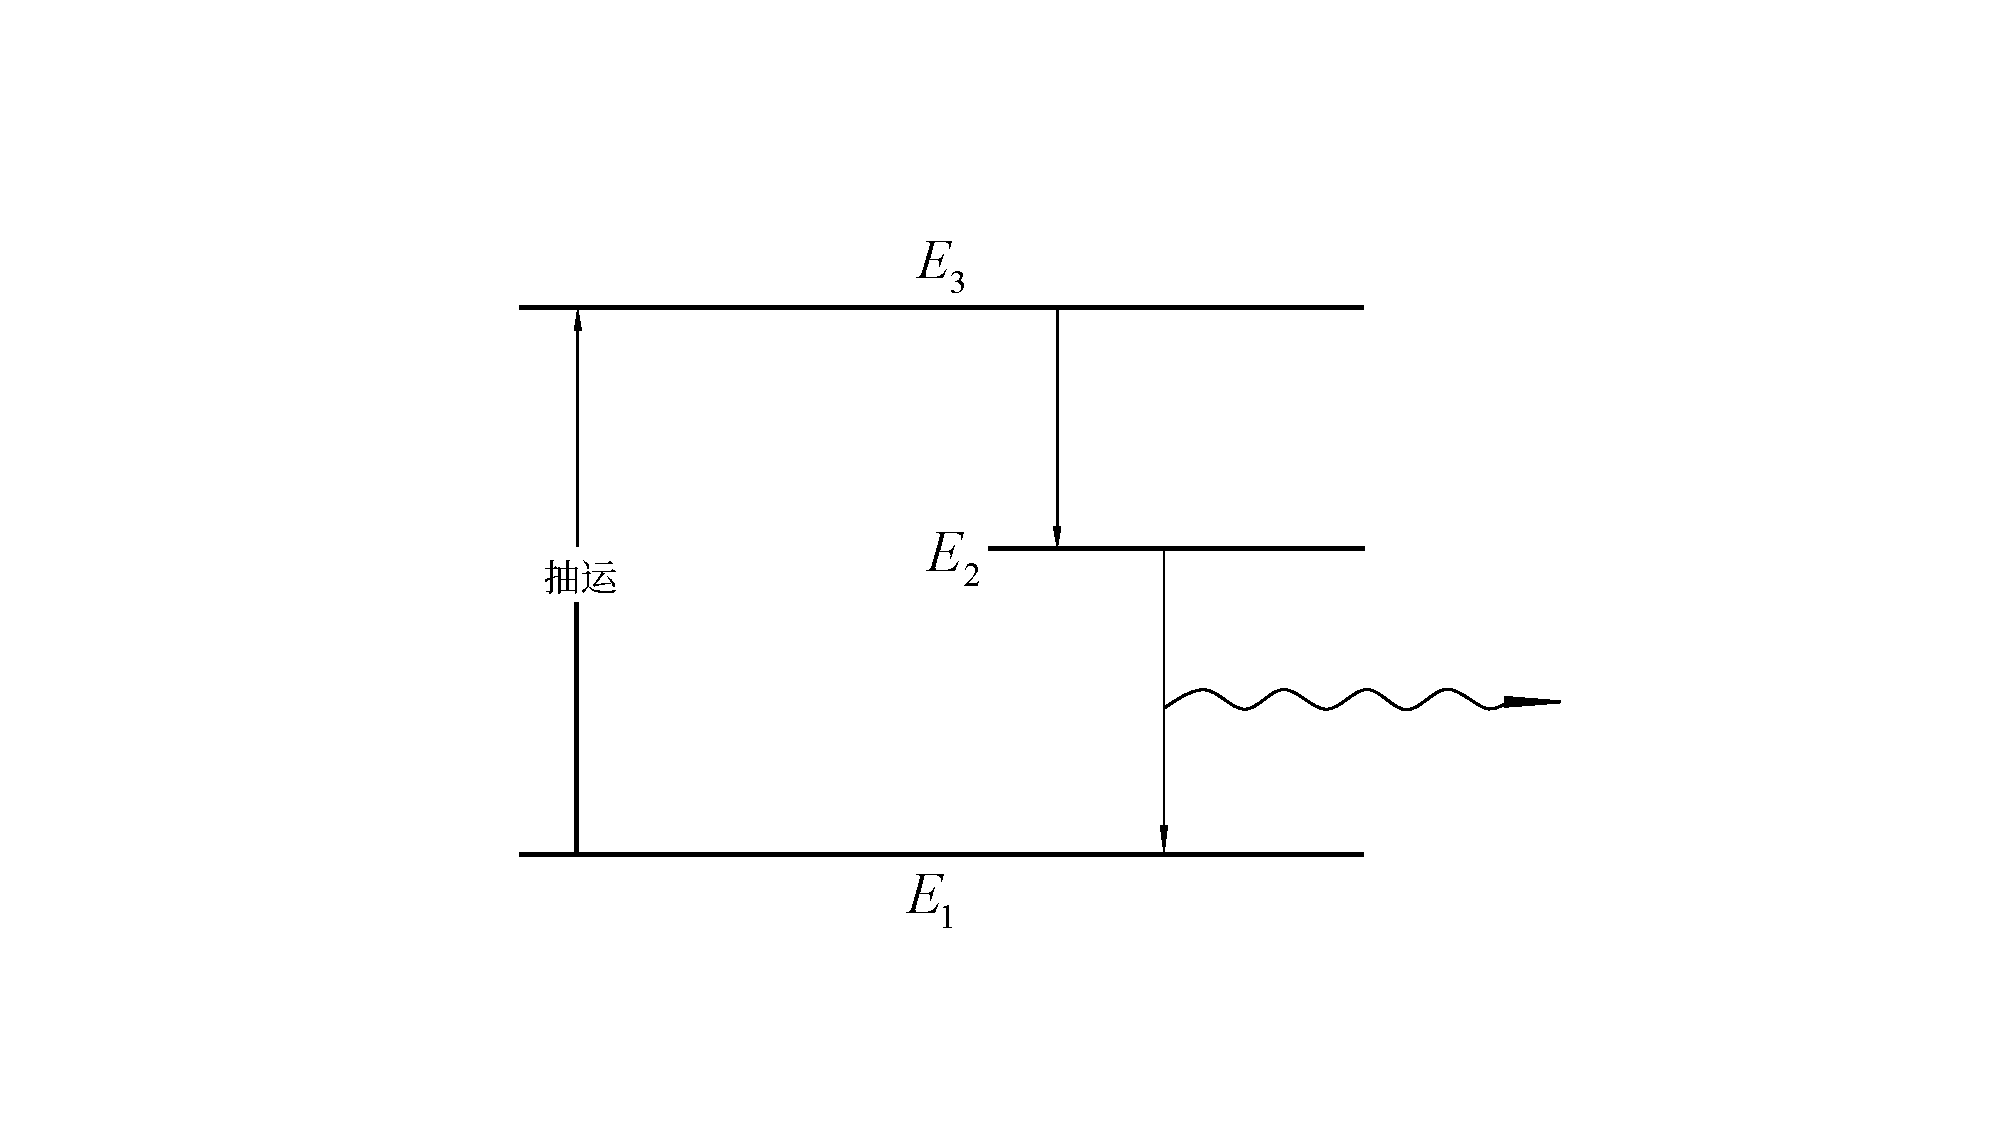
\includegraphics[width=4cm,clip]{QM file/figure/9-3}
	\caption{}\label{fig.9-3}
\end{wrapfigure}
第一代激光器是固体脉冲式,典型代表就是最早出现的红宝石激光器.红宝石是$\ce{Al_{2}O_{3}}$,渗有约0.04\%的\ce{Cr}.利用$\ce{Cr^{+++}}$离子的三能级系统产生激光.这三个能级如图\ref{fig.9-3}所示.用闪光氙灯照射红宝石棒,使$\ce{Cr^{+++}}$从基态能级$E_{1}$上升到$E_{3}$,这个过程称为抽运.$E_{3}$能级经由自发跃迁降到$E_{2}$(寿命约$10^{-7}\si{s}$),$E_{2}$是亚稳态,它与$E_{1}$间的自发跃迁寿命约$10^{-3}\si{s}$.$E_{2}$和$E_{1}$就是用来产生激光的工作能级.如来自氙灯的激发光足够强,在一次闪光时间内$(<10^{-3}\si{s})$就能在上能级$E_{2}$集聚起足够多的$\ce{Cr^{+++}}$离子,实现能级$E_{2}$,$E_{1}$间粒子数反转.红宝石棒的两端面做成平行反射面,(一端有10\%透射率,以获得激光输出)棒本身就是谐振腔.使$E_{2},E_{1}$间产生受激跃迁的最初光讯号就是自发跃迁产生的少数沿棒的轴向传播的光子$(\hbar\omega_{21})$,在两反射面间来回振荡,同时激发更多的$\ce{Cr^{+++}}$离子实现$E_{2}\rightarrow E_{1}$受激辐射,使腔内光讯号迅速放大,成为很强的平行光束,从一端射出这种激光器能量转换(氙灯光能$\rightarrow$激光输出)效率较低,在0.1\%以下.氙灯的每一次闪光,产生一次脉冲式激光(波长\num{694.3}\si{nm})输出,因为是脉冲式,输出激光的单色性并不很好.

能够连续地产生激光,单色性较好的是氦-氖激光器,它利用\ce{Ne}原子的特殊能级构造产生激光,能级图如图\ref{fig.9-4}所示.
\begin{figure}[!h]
	\centering
	\small
	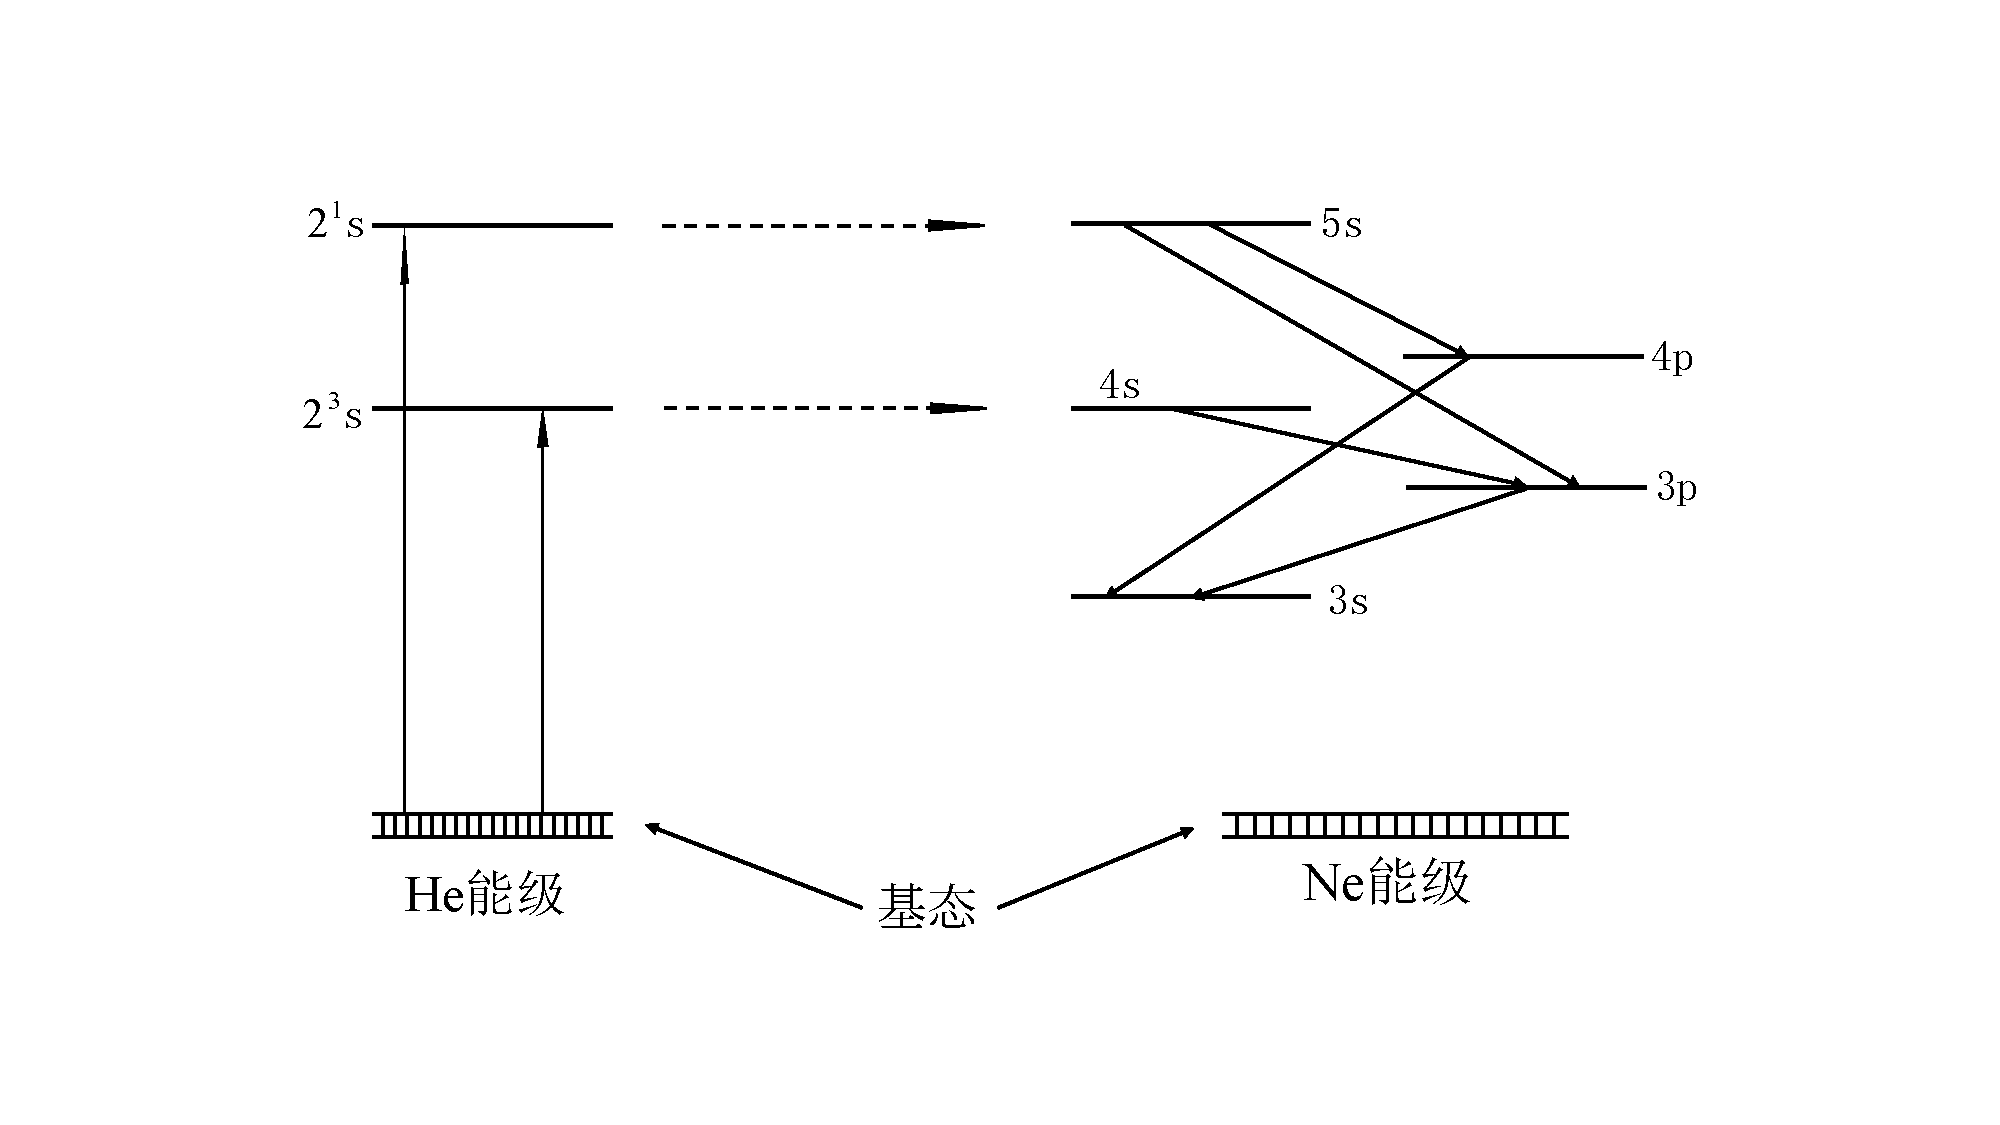
\includegraphics[width=6cm,clip]{QM file/figure/9-4}
	\caption{}\label{fig.9-4}
\end{figure}
\noindent 氦氖激光管中氦与氖约为5:1到10:1,管的两端加上$2\sim3\si{kV}$电压,使产生气体放电,电子的撞击使\ce{He}的一个电子被激发到$2^{1}\si{s}$或$2^{3}\si{s}$能级,再通过气体原子间的碰撞将能量转移给\ce{Ne}原子,使其处于单电子激发能级5s和4s(这两个能级恰好与\ce{He}的$2^{1}\si{s}$及$2^{3}\si{s}$能级接近,容易发生能量转移.)\ce{Ne}原子产生激光的能级跃迁是5s$\rightarrow$4p,5s$\rightarrow$3p,及4s$\rightarrow$3p,由于4p及3p能级原来是空的(\ce{Ne}原子集中在基态能级上),这样就很顺利地实现了上能级与下能级之间的原子数反转.完成受激辐射过程而到达4p及3p能级的原子,可以经由自发跃迁迅速降到3s能级,再经过碰撞降到基态,这样在下能级(4p,3p)就不会积累原子,所以产生激光的过程可以连续进行.造成谐振腔的反射镜可以放在管外,便于调节.氦氖激光有极好的单色性,如\ce{Ne}的5s$\rightarrow$3p跃迁产生的波长\num{632.8}\si{nm}的红光,$\frac{\Delta\nu}{\nu}\sim\num{1.6}\times10^{-11}$.最好的激光$\frac{\Delta\nu}{\nu}$仅$10^{-14}$.

激光器种类很多,发展很快,这里就不多介绍了.


% 能量-时间不确定度关系
\starthis\section[能量-时间不确定度关系]{能量-时间不确定度关系} \label{sec:09.06} % 
% \makebox[5em][s]{} % 短题目拉间距

微观过程的某些性质常可用“能量-时间不确定度关系”来解释.这个“不确定度关系”的一般表达方式是
\eqshort
\begin{empheq}{equation}\label{eq96.1}
	\Delta E\Delta t\gtrsim\hbar
\end{empheq}\eqnormal
$\Delta E,\Delta t$分别代表能量和时间的不确定度.由于能量是力学量,$\Delta E$可以尽量按精确的意义理解,其严格定义是
\begin{empheq}{equation}\label{eq96.2}
	(\Delta E)^{2}=\overline{E^{2}}-\overline{E}^{2}
\end{empheq}\eqshort
而时间并非力学量,对于过程的时间不确定度,一般仅作量级估算.因此\eqref{eq96.1}式也仅在量级意义上使用.我们将先讨论几个典型实例,借以说明\eqref{eq96.1}式的正确性,然后再稍作理论探讨.


\exa 原子自发辐射,初态$\varPsi_{2}\rightarrow$终态$\varPsi_{1}(E_{2}-E_{1}>0)$设在$t=0$制备好大量处于初态$\varPsi_{2}$的原子,然后就测量辐射的光子能量$E=\hbar\omega$.设跃迁$\varPsi_{2}\rightarrow\varPsi_{1}$的平均寿命为$\tau$,有效测量大致在$t=\tau$前完成,可取$\Delta t\sim\tau$.被测量的光子,其空间分布范围大致是$\Delta x\lesssim c\tau$,因此有动量不定值$\Delta p\sim\frac{\hbar}{\Delta x}\gtrsim\frac{\hbar}{c\tau}$,和能量不定值$\Delta E=c\Delta p\gtrsim\frac{\hbar}{\tau}$.结论是:测到的光子能量$\hbar\omega$并不严格地等于原子跃迁前后的能级差$(E_{2}-E_{1})$,而有不确定度$\Delta E$,而$\Delta E$,$\Delta t$满足\eqref{eq96.1}式.

表面看来,以上结论与能量守恒定律有矛盾,其实不然.到测得光子时为止,原子在终态$\varPsi_{1}$中停留的时间是有限的$(t\lesssim\tau)$所以终态并非严格意义下的定态,其能量值并不严格等于$E_{1}$,而有分布宽$\Delta E\gtrsim\frac{\hbar}{\tau}$,初态也有类似的能级宽度.初、终态的能级宽度正是光子能量不确定度的来由.总之,如某状态只在有限时间内存在,它就不是严格的定态,而有能量分布$\Delta E$.

\exa 在粒子物理研究中发现,能够自行蜕变的不稳定粒子,其质量都有不确定度$\Delta m$,它与蜕变的平均寿命$\tau$有关系
\begin{empheq}{equation}\label{eq96.3}
	\Delta m\cdot\tau\sim\frac{\hbar}{c^{2}}
\end{empheq}\eqnormal
用能量-时间不确定关系\eqref{eq96.1}式容易解释这个关系,因为粒子质量与相对论性质的能量有关系$E=mc^{2}$,所以$\Delta E=c^{2}\Delta m$,而寿命$\tau$正是时间不确定度$(\Delta t\sim\tau)$.

\exa 在单频微扰作用下原子从初态$\varPsi_{k}$(能级$E_{k}$)向终态$\varPsi_{f}$(能级$E_{f}$)跃迁.跃迁概率由\eqref{eq92.5}式表示.考虑终态能量连续的情形,对于$F_{fk}$相同而能量互相不同的终态,跃迁概率与初终态能级差$(E_{f}-E_{k})=\hbar\omega_{fk}$有关系
\begin{empheq}{align*}
	|C_{f}(t)|^{2} &\propto\frac{[1-\cos(\omega_{fk}-\omega_{o})t]}{(\omega_{fk}-\omega_{o})^{2}}	\\
	&\propto \frac{\sin^{2}[(\omega_{fk}-\omega_{o})t/2]}{(\omega_{fk}-\omega_{o})^{2}}
\end{empheq}\eqshort
$|C_{f}(t)|^{2}-\omega_{fk}$关系如图\ref{fig.9-5}所示.$\omega_{fk}$的有效分布宽度大致可以确定为$\Delta\omega_{fk}\sim\frac{2\pi}{t}$,因此终态能量不确定度约为$\Delta E_{f}\sim\frac{2\pi\hbar}{t}$,即
\begin{empheq}{equation}\label{eq96.4}
	\Delta E_{f}\cdot\sim2\pi\hbar
\end{empheq}\eqnormal

\begin{figure}[!h]
	\centering
	\small
	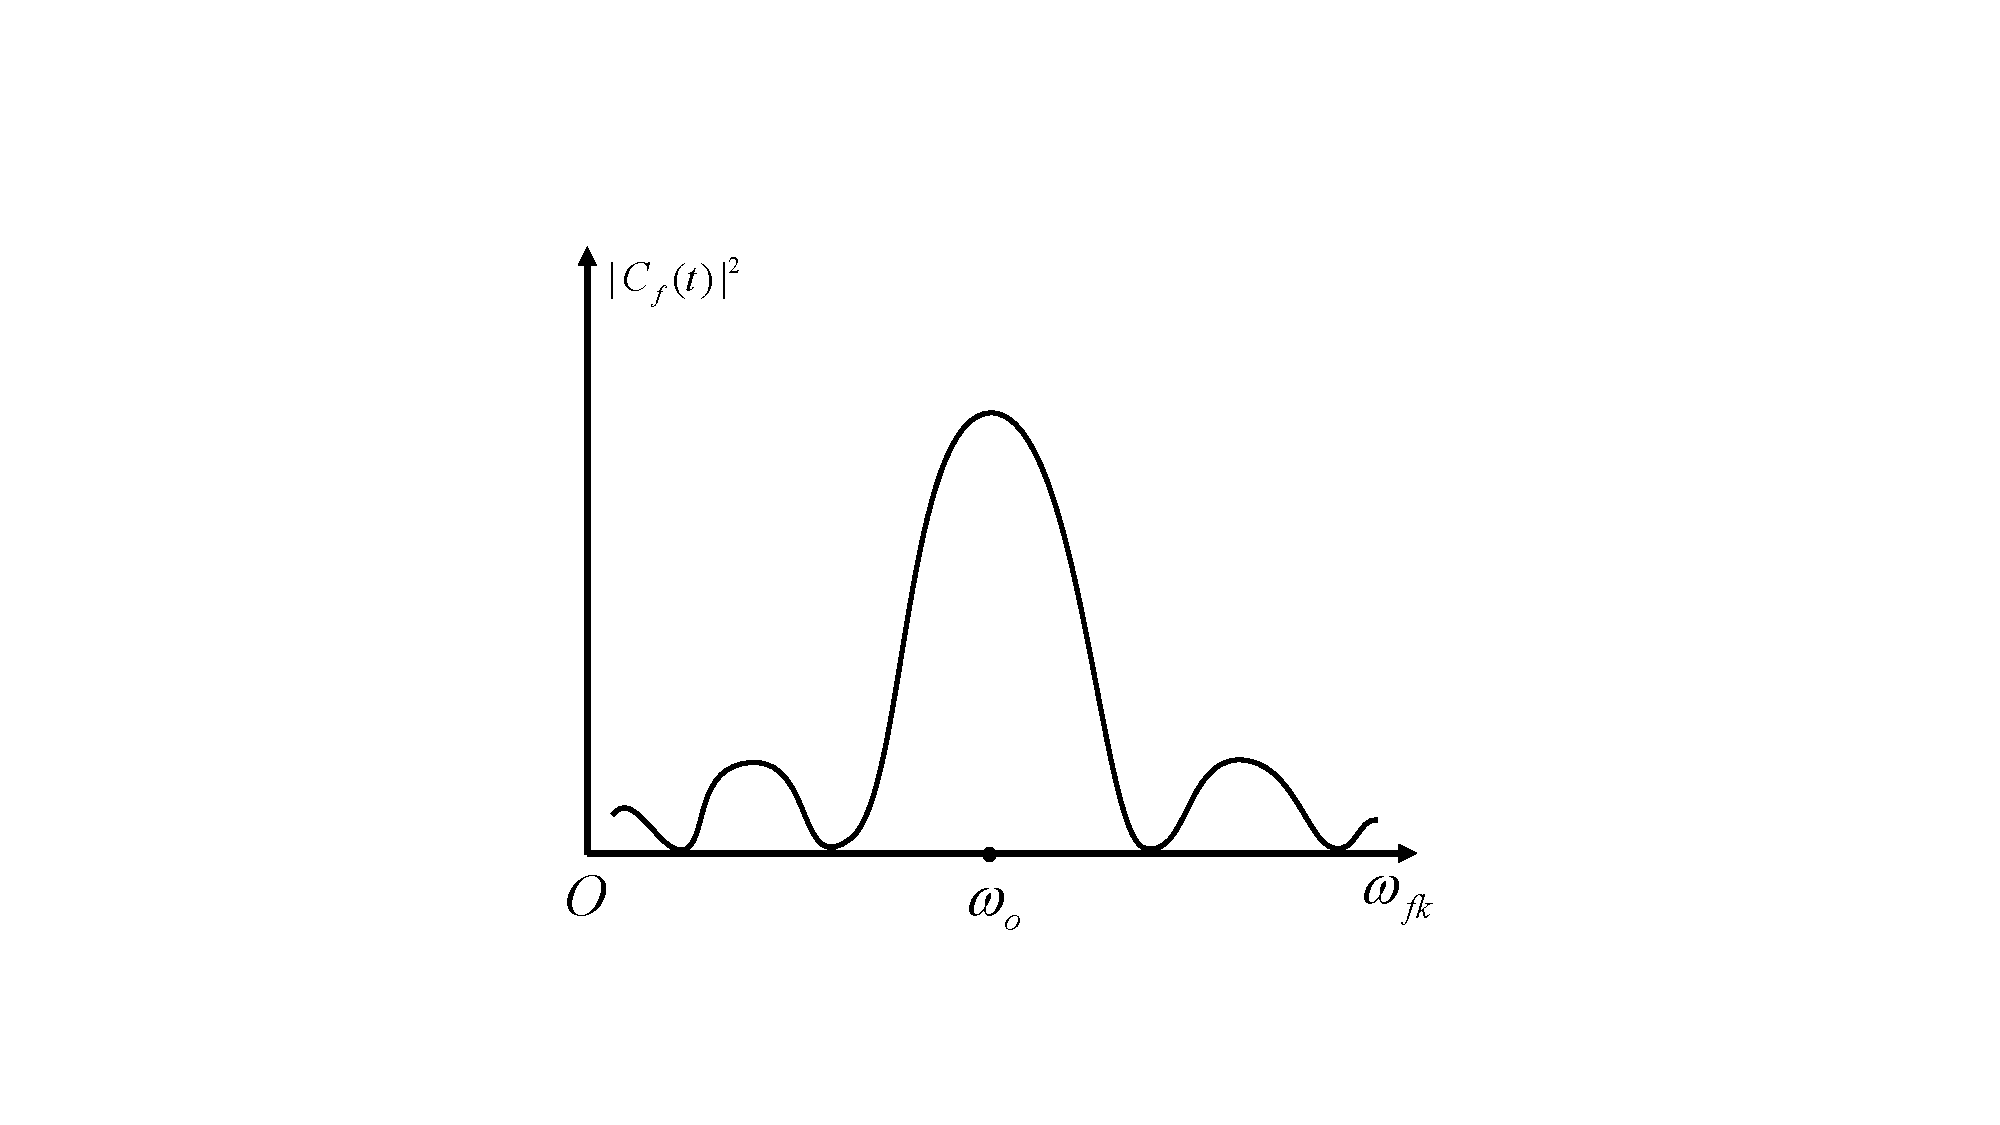
\includegraphics[width=5cm,clip]{QM file/figure/9-5}
	\caption{}\label{fig.9-5}
\end{figure}
\noindent 这里$t$相当于终态存在时间的不确定度,即$\Delta t$.造成终态能量不完全确定的原因是:微扰$H^{\prime}$既然只在有限时间内起作用,它实质上不是严格的单频微扰,其频谱宽度$\Delta\omega\gtrsim\frac{2\pi}{t}$,因此原子从$H^{\prime}$吸收的能量量子并不严格等于$\hbar\omega$,而有不确定度$\hbar\Delta\omega\gtrsim\frac{2\pi\hbar}{t}$,所以终态能量也有同样的不确定度.

在例1和例3中,$\Delta E$都很小,常可略去不计.例如例3,取$t\sim10^{-10}\si{s}$,则$\Delta E_{f}\sim\frac{\hbar}{t}\sim4\times10^{-5}\si{eV}$.$\S$\ref{sec:09.02}正是在忽略$\Delta E_{f}$的条件下,对跃迁速率作了近似处理,从而得出$E_{f}=E_{k}+\hbar\omega$的结论.但是例2中$\tau$有时非常小,$\Delta m$可以达到$m$的量级.

能量-时间不确定度关系的正确性是肯定的,对它的论证却并不统一.常见的一种论证是,取能量算符为$\hat{E}=i\hbar\frac{\partial}{\partial t}$,于是就有
\begin{empheq}{equation}\label{eq96.5}
	[t,\hat{E}]=[t,i\hbar\frac{\partial}{\partial t}]=-i\hbar
\end{empheq}\eqshort
再仿照$x-p_{x}$不确定关系的推导,得到
\begin{empheq}{equation*}
	\Delta E\cdot\Delta t\geqslant\frac{\hbar}{2}
\end{empheq}\eqnormal
这种论证显然不妥.我们姑且不去争论$t$是否可以作为算符对待,至少可以指出将$i\hbar\frac{\partial}{\partial t}$作为能量算符用于对易式的计算是不妥的,容易引申出种种谬论.例如,对于任何不显含$t$的算符$\hat{F}(\boldsymbol{r},\boldsymbol{p}$,显然有$\left[\hat{F},\frac{\partial}{\partial t}\right]=\frac{\partial\hat{F}}{\partial t}$,因此$F$是守恒量,等等.

利用狭义相对论中四维协变矢量的概念来论证能量-时间不确定关系也许是较好的办法.在相对论中,
\begin{empheq}{equation*}
	x_{\mu}=(x,y,z,ict),\quad p_{\mu}=\left(p_{x},p_{y},p_{z},\frac{iE}{c}\right)
\end{empheq}\eqshort
众所周知,利用$\hat{p_{x}}=-i\hbar\frac{\partial}{\partial x}$可以证明$x-p_{x}$不确定度关系:
\begin{empheq}{equation}\label{eq96.6}
	\Delta x\cdot\Delta p_{x}\geqslant\frac{\hbar}{2}
\end{empheq}
由于$\hat{p_{x}}=-i\hbar\frac{\partial}{\partial x}$也适用于相对论情形,所以\eqref{eq96.6}式也适用于相对论情形.$y-p_{y},z-p_{z}$间也有类似的不确定度关系.据此类推,$x_{4}=ict$与$p_{4}=\frac{iE}{c}$之间也应有不确定度关系:
\begin{empheq}{equation*}
	\Delta x_{4}\cdot\Delta p_{4}\geqslant\frac{\hbar}{2}
\end{empheq}
亦即
\begin{empheq}{equation} \label{eq96.7}
	\Delta t\cdot\Delta E\geqslant\frac{\hbar}{2}
\end{empheq}\eqnormal
在量级的意义上,\eqref{eq96.7}式与\eqref{eq96.1}式并无不同



% 习题
\begin{exercises}
	
\exercise 设$t<0$时体系处于基态$\varPsi_{1}$,$t>0$时受到逐渐增强再逐渐消退的外来微扰$H^{\prime}(x,t)$作用,
\begin{empheq}{equation*}
	H^{\prime}(x,t)=\frac{F(x)}{[\tau^{2}+(t-t_{0})^{2}]},\quad \frac{t_{0}}{\tau}\gg1
\end{empheq}

设$t_{0}$很大,满足$\dfrac{(E_{2}-E_{1})t_{0}}{\hbar}\gg2\pi$.求微扰消退后$(t\rightarrow\infty)$体系处于各激发态$[\varPsi_{n}(x)]$的概率.
	
\exercise 某体系(能量算符$H_{0}$)只有两个能级(非简并的),$E_{2}-E_{1}=\hbar\omega>0$,设$t<0$时处于基态$\varPsi_{1}$.$t>0$时受到外来作用,能量算符变成$H=H_{0}+H^{\prime}$,设$H^{\prime}$不含$t$,矩阵元为
\begin{empheq}{align*}
	\langle\varPsi_{1}|H^{\prime}|\varPsi_{1}\rangle&=\langle\varPsi_{2}|H^{\prime}|\varPsi_{2}\rangle=0,	\\
	\langle\varPsi_{1}|H^{\prime}|\varPsi_{2}\rangle&=\langle\varPsi_{2}|H^{\prime}|\varPsi_{1}\rangle=\hbar\nu
\end{empheq}

试严格求解薛定谔方程,求$\varPsi(t)$.如在任意$t>0$时刻测量$H_{0}$之值,测得$H_{0}=E_{2}$的概率等于什么?

[提示:先求出$H$的本征函数$\varPsi_{\alpha},\varPsi_{\beta}$,本征值$E_{\alpha},E_{\beta}$,再将$\varPsi(t)$表示成也$\varPsi_{\alpha},\varPsi_{\beta}$的叠加,求出$\varPsi(t)$后,再表示成$\varPsi_{1},\varPsi_{2}$的叠加.]

\exercise 上题中,设$H^{\prime}$是微扰,即设$\nu\ll\omega$,求$t>0$时刻测得$H_{0}=E_{2}$的概率,与微扰论结果[\eqref{eq91.12}式]比较.

\exercise $t=0$时电子的自旋取值为$S_{z}=\dfrac{\hbar}{2}$,$t>0$时受到沿正$x$轴方向的磁场$(\boldsymbol{B})$作用,作用势为
\begin{empheq}{equation*}
	H^{\prime}=\frac{e B}{m_{e}c}S_{z}=\hbar\omega\sigma_{x},\quad \omega=\frac{e B}{2m_{e}c}
\end{empheq}

视$H^{\prime}$为微扰,用\eqref{eq91.12}式计算$t>0$时测得$S_{z}=-\dfrac{\hbar}{2}$的概率.微扰论计算公式成立的条件是什么?(本题是在简并态之间的跃迁问题,请与7-20题结果对照.)

\exercise 电荷为$e$(或$-e$)质量为$m$的一维谐振子,(a) 写出电偶极跃迁选择定则.(b) 求自发跃迁速率公式(初态$\varPsi_{n}$).
	
\exercise 电荷为$e$(或$-e$)质量为$m$的三维各向同性谐振子,[用直角坐标系,以$\varPsi_{n1}(x)\varPsi_{n2}(x)\varPsi_{n3}(x)$作为能量本征函数.](a) 求电偶极跃迁选择定则,(b) 求自发跃迁速率公式.(设初态量子数$n_{1}=n_{2}=n_{3}=n$,考虑向一切可能的终态跃迁速率之和.)(c) 取$n_{1}=n_{2}=n_{3}=1$,如谐振子是电子,$\hbar\omega=1\si{eV}$,求初态平均寿命.如谐振子是质子,$\hbar\omega=1\si{MeV}$,求初态平均寿命.
	
\exercise 处于无限深平底势阱中的带电粒子,求其电偶极跃迁选择定则.
	
\exercise 考虑自旋轨道耦合,原子中价电子(最外层电子)定态波函数取$(H,\boldsymbol{L}^{2},\boldsymbol{J}^{2},J_{z})$共同本征函数,量子数$(nljm_{j})$.对于价电子的自发跃迁(电偶极跃迁),证明选择定则是
\begin{empheq}{equation*}
	\Delta l=\pm1,\quad \Delta j=0,\pm1,\quad \Delta m_{j}=0,\pm1
\end{empheq}

[提示:利用公式$\boldsymbol{\sigma}(\boldsymbol{\sigma}\cdot\boldsymbol{r})+(\boldsymbol{\sigma}\cdot\boldsymbol{r})\boldsymbol{\sigma}=2r$,以及7-15题证明的公式.注意$\boldsymbol{r},\boldsymbol{\sigma}\cdot\boldsymbol{r}$及$Y_{lm}$的宇称性.要着重证明$\Delta j=\pm2$的跃迁是禁止的.]

\exercise 大量氢原子均处于基态,而且电子自旋均沿正$z$轴方向极化,即电子处于$(n,l,m,m_{s})=\left(1,0,0,\dfrac{1}{2}\right)$状态,亦即$(n,l,j,m_{j})=\left(1,0,\dfrac{1}{2},\dfrac{1}{2}\right)$状态.今用电场沿$\pm z$轴方向偏振的线偏振光照射这些原子,造成1s$\rightarrow$2p能级跃迁,忽略2p$_{1/2}$态与2p$_{3/2}$态的能量差.[取相同的径向波函数$R_{21}(r)$]试利用上题证明的选择定则确定终态$(n=2)$量子数$ljm_{j}$的可能取值,并计算终态为2p$_{1/2}$和2p$_{3/2}$的分支比(原子数之比).
	
\exercise 以磁场$\boldsymbol{B}(t)$作用于原子,引起价电子状态的跃迁,求量子数$(lmm_{s})$及$(ljm_{j})$的选择定则.
	
\end{exercises}


% 第十章 多粒子体系
\chapter{多粒子体系}\label{chp:10}
% \makebox[5em][s]{} % 短题目拉间距

本章讨论多粒子体系的量子力学问题,尤其是二体问题.全同粒子的存在是微观物质世界的特点,有关全同粒子体系的讨论是本章的中心内容.

% 二粒子体系
\section[二粒子体系]{二粒子体系} \label{sec:10.01} % 
% \makebox[5em][s]{} % 短题目拉间距

考虑两个粒子组成的体系,设粒子质量为$m_{1},m_{2}$,坐标为$\boldsymbol{r}_{1}(x_{1},y_{1},z_{1})$,$\boldsymbol{r}_{2}(x_{2},y_{2},z_{2})$.为了简明,暂不考虑自旋自由度,并设两粒子间的相互作用势是相对距离的函数,即
\begin{empheq}{equation}\label{eqx1.1}
	V_{12}=V(r),\quad r=|\boldsymbol{r}_{1}-\boldsymbol{r}_{2}|
\end{empheq}
在没有外场作用的情况下,这二粒子体系的总能量算符为
\begin{empheq}{align}\label{eqx1.2}
	H &=\frac{\boldsymbol{p}_{1}^{2}}{2m_{1}}+\frac{\boldsymbol{p}_{2}^{2}}{2m_{2}}+V(r)	\nonumber\\
	&=-\frac{\hbar^{2}}{2m_{1}}\nabla_{1}^{2}-\frac{\hbar^{2}}{2m_{2}}\nabla_{2}^{2}+V(r)
\end{empheq}
其中$\boldsymbol{p}_{1},\boldsymbol{p}_{2}$是粒子1,2的动量算符,
\begin{empheq}{equation}\label{eqx1.3}
	\begin{aligned}
		\boldsymbol{p}_{1}&=-i\hbar\nabla_{1},\quad p_{1x}=-i\hbar\frac{\partial}{\partial x_{1}}	\\
		\boldsymbol{p}_{2}&=-i\hbar\nabla_{2},\quad p_{2x}=-i\hbar\frac{\partial}{\partial x_{2}}
	\end{aligned}
\end{empheq}\eqshort
体系的状态由波函数$\Psi(\boldsymbol{r}_{1},\boldsymbol{r}_{2},t)$描述,$\Psi$满足薛定谔方程
\begin{empheq}{equation}\label{eqx1.4}
	i\hbar\frac{\partial}{\partial t}\Psi=H\Psi
\end{empheq}\eqnormal

引入质心坐标$\boldsymbol{R}(X,Y,Z)$,相对坐标$\boldsymbol{r}(x,y,z)$和折合质量$\mu$,它们的定义与
经典力学定义相同,即
\begin{empheq}{align}
	\frac{1}{\mu} &=\frac{1}{m_{1}}+\frac{1}{m_{2}},\quad \mu=\frac{m_{1}m_{2}}{m_{1}+m_{2}}		\label{eqx1.5}\\ 
	\boldsymbol{R}&=\frac{m_{1}\boldsymbol{r}_{1}+m_{2}\boldsymbol{r}_{2}}{m_{1}m_{2}}=\mu\left(\frac{\boldsymbol{r}_{1}}{m_{1}}+\frac{\boldsymbol{r}_{2}}{m_{2}}\right)	\label{eqx1.6}\\
	\boldsymbol{r} &=\boldsymbol{r}_{1}-\boldsymbol{r}_{2}\quad \text{即}x=x_{1}-x_{2},\cdots		\label{eqx1.7}
\end{empheq}\eqlong
容易证明下列微分关系:
\begin{empheq}{align}\label{eqx1.8}
	\frac{\partial}{\partial x_{1}} &=\frac{\partial X}{\partial x_{1}}+\frac{\partial}{\partial X}+\frac{\partial x}{\partial x_{1}}\frac{\partial}{\partial x}=\frac{\mu}{m_{2}}\frac{\partial}{\partial X}+\frac{\partial}{\partial x}	\nonumber\\
	\frac{\partial}{\partial x_{2}} &=\frac{\partial X}{\partial x_{2}}+\frac{\partial}{\partial X}+\frac{\partial x}{\partial x_{2}}\frac{\partial}{\partial x}=\frac{\mu}{m_{1}}\frac{\partial}{\partial X}+\frac{\partial}{\partial x}
\end{empheq}\eqnormal
因此总动量算符可以表示成
\begin{empheq}{align}\label{eqx1.9}
	P_{x}&=p_{1x}+p_{2x}	\nonumber\\
	&=-i\hbar\left(\frac{\partial}{\partial x_{1}}+\frac{\partial}{\partial x_{2}}\right)=-i\hbar\frac{\partial}{\partial X}
\end{empheq}
\begin{empheq}{align*}\label{eqx1.9'}
	\boldsymbol{P}&=\boldsymbol{p}_{1}+\boldsymbol{p}_{2}	\\
	&=-i\hbar(\nabla_{1}+\nabla_{2})=-i\hbar\nabla_{n}	\tag{$10.1.9^{\prime}$}
\end{empheq}
定义相对动量算符
\begin{empheq}{equation}\label{eqx1.10}
	\boldsymbol{p}=-i\hbar\nabla,\quad \text{即}p_{x}=-i\hbar\frac{\partial}{\partial x},\cdots
\end{empheq}
利用\eqref{eqx1.8}式,易得
\begin{empheq}{equation}\label{eqx1.11}
	\boldsymbol{p}=\frac{\mu}{m_{1}}\boldsymbol{p}_{1}-\frac{\mu}{m_{2}}\boldsymbol{p}_{2}
\end{empheq}
[经典力学中也有类似关系相对动量的经典力学定义是
\begin{empheq}{equation*}
	\boldsymbol{p}=\mu\frac{d\boldsymbol{r}}{dt}=\mu\frac{d\boldsymbol{r}_{1}}{dt}-\mu\frac{d\boldsymbol{r}_{2}}{dt}
\end{empheq}
由于
\begin{empheq}{equation*}
	\boldsymbol{p}_{1}=m_{1}\frac{d\boldsymbol{r}_{1}}{dt},\quad \boldsymbol{p}_{2}=m_{2}\frac{d\boldsymbol{r}_{2}}{dt}
\end{empheq}
显然仍有\eqref{eqx1.11}式的关系.]

注意,$\boldsymbol{p}_{1},\boldsymbol{p}_{2},\boldsymbol{P},\boldsymbol{p}$是互相对易的算符.利用\eqref{eqx1.9'}及\eqref{eqx1.11}式,体系的总动能算符可以表示成
\begin{empheq}{equation}\label{eqx1.12}
	\boxed{	\frac{\boldsymbol{p}_{1}^{2}}{2m_{1}}+\frac{\boldsymbol{p}_{2}^{2}}{2m_{2}}=\frac{\boldsymbol{P}^{2}}{2(m_{1}m_{2})}+\frac{\boldsymbol{p}^{2}}{2\mu}	}
\end{empheq}
经典力学中也有这样的关系.体系的总能量算符可以表示成
\begin{empheq}{align}\label{eqx1.13}
	H &=\frac{\boldsymbol{P}^{2}}{2(m_{1}m_{2})}+\frac{\boldsymbol{p}^{2}}{2\mu}+V(r)	\nonumber\\
	&=-\frac{\hbar^{2}}{2(m_{1}+m_{2})}\nabla_{R}^{2}-\frac{\hbar^{2}}{2\mu}\nabla^{2}+V(r)
\end{empheq}
第一项是质心动能算符,后两项是相对运动的动能和势能算符,其中势能$V(r)$只与相对坐标有关.薛定谔方程\eqref{eqx1.4}式的分离变量特解(定态)显然可以表示成
\begin{empheq}{equation}\label{eqx1.14}
	\Psi=\phi(\boldsymbol{R})\varPsi(\boldsymbol{r})e^{-iEt/\hbar}
\end{empheq}
其中$\phi(\boldsymbol{R})$和$\varPsi(\boldsymbol{r})$分别描述质心运动和相对运动,并满足本征方程
\begin{empheq}{align}
	&-\frac{\hbar^{2}}{2(m_{1}+m_{2})}\nabla_{R}^{2}\phi(\boldsymbol{R})=E_{c}\phi(\boldsymbol{R})		\label{eqx1.15}\\
	&-\frac{\hbar^{2}}{2\mu}\nabla^{2}\varPsi(\boldsymbol{r})+V(r)\varPsi(\boldsymbol{r})=(E-E_{c})\varPsi(\boldsymbol{r})		\label{eqx1.16}
\end{empheq}
\eqref{eqx1.15}式表明质心运动等效于一个质量为$(m_{1}+m_{2})$的粒子的自由运动,动能$E_{c}\geqslant0$,\eqref{eqx1.15}式的平面波解为
\begin{empheq}{equation}\label{eqx1.17}
	\phi(\boldsymbol{R})=e^{i\boldsymbol{k}\cdot\boldsymbol{R}},\quad E_{c}=\frac{\hbar^{2}k^{2}}{2(m_{1}+m_{2})}
\end{empheq}
这也是总动量$\boldsymbol{P}$的本征函数,本征值$\boldsymbol{P}=\hbar\boldsymbol{k}$.

\eqref{eqx1.16}式表明相对运动等价于质量为$\mu$的粒子在势场$V(r)$中的运动,相应的能盘为$(E-E_{c})$,$E$是体系的总能量.对于氢原子(参看$\S$\ref{sec:05.04}),$m_{1}=m_{e},m_{2}=m_{p}$,由于$\frac{m_{p}}{m_{e}}\approx\num{1836}$,所以
\begin{empheq}{equation*}
	\mu=\frac{m_{e}m_{p}}{m_{e}+m_{p}}\approx\frac{1836}{1837}m_{e}
\end{empheq}
总之,如$m_{2}\gg m_{1}$,则$\mu$接近并稍小于$m_{1}$.

二粒子体系的总轨道角动量算符为
\begin{empheq}{equation}\label{eqx1.18}
	\boldsymbol{L}_{\text{总}}=\boldsymbol{L}_{1}+\boldsymbol{L}_{2}=\boldsymbol{r}_{1}\times\boldsymbol{p}_{1}+\boldsymbol{r}_{2}\times\boldsymbol{p}_{2}
\end{empheq}
如根据\eqref{eqx1.6}式与\eqref{eqx1.7}式用质心坐标$\boldsymbol{R}$和相对坐标$\boldsymbol{r}$表示$\boldsymbol{r}_{1}$与$\boldsymbol{r}_{2}$,根据\eqref{eqx1.9'}式与\eqref{eqx1.11}式用质心动量(总动量)$\boldsymbol{P}$和相对动量$\boldsymbol{p}$表示$\boldsymbol{p}_{1}$与$\boldsymbol{p}_{2}$,容易得到
\begin{empheq}{equation}\label{eqx1.19}
	\boldsymbol{L}_{\text{总}}=\boldsymbol{R}\times\boldsymbol{P}+\boldsymbol{r}\times\boldsymbol{p}=\boldsymbol{L}_{c}+\boldsymbol{L}
\end{empheq}
其中
\begin{empheq}{equation}\label{eqx1.20}
	\boldsymbol{L}_{c}=\boldsymbol{R}\times\boldsymbol{P},\quad \boldsymbol{L}=\boldsymbol{r}\times\boldsymbol{p}
\end{empheq}
$\boldsymbol{L}_{c}$称为质心角动量,$\boldsymbol{L}$称为相对角动量.\eqref{eqx1.18}至\eqref{eqx1.20}式在经典力学中也是成立的.

在经典力学中,采用“质心坐标系”意味着以质心作为坐标系原点,因此$\boldsymbol{R}=0,\boldsymbol{P}=0,\boldsymbol{L}_{c}=0$.

在量子力学中,$\boldsymbol{R}$和$\boldsymbol{P}$是不对易的,在任何状态下$\boldsymbol{R}$和$\boldsymbol{P}$不能同时取确定值.采用“质心坐标系”意指总动量$\boldsymbol{P}$的本征值为0,即$\boldsymbol{P}\Psi=0$,这相当于\eqref{eqx1.17}式中$\boldsymbol{k}=0$,而$\Psi=\varPsi(\boldsymbol{r},t)$,与$\boldsymbol{R}$无关.这时$\boldsymbol{R}\times\boldsymbol{P}\Psi=0$,即质心角动量$\boldsymbol{L}_{c}$的取值也为0.在这种意义上可以认为$\boldsymbol{L}_{\text{总}}=\boldsymbol{L}$.

\pskip
\example 按照力学量算符的海森堡运动方程[\eqref{eq39.15}式]
\eqshort
\begin{empheq}{equation*}
	\frac{d\hat{A}}{dt}=\frac{1}{i\hbar}[\hat{A},\hat{H}]
\end{empheq}\eqlong
求二粒子体系$\boldsymbol{R},\boldsymbol{r},\boldsymbol{P},\boldsymbol{p},\boldsymbol{L}_{c},\boldsymbol{L}$等力学量算符的时间变化规律.

\solution 总能量算符$H$的表达式\eqref{eqx1.2}和\eqref{eqx1.13},显然用\eqref{eqx1.13}式方便.由于$V(r)$与$\boldsymbol{R}$无关,$\boldsymbol{p}$与$\boldsymbol{R}$对易,所以
\begin{empheq}{align}
	\frac{d\boldsymbol{R}}{dt} &=\frac{1}{2i\hbar(m_{1}+m_{2})}[\boldsymbol{R},\boldsymbol{P}^{2}]=\frac{\boldsymbol{P}}{m_{1}+m_{2}}			\label{eqx1.21}\\
	\frac{d\boldsymbol{P}}{dt} &=\frac{1}{i\hbar}[\boldsymbol{P},V(r)]=0	\label{eqx1.22}\\
	\frac{d\boldsymbol{L}_{c}}{dt} &=\frac{d\boldsymbol{R}}{dt}\times\boldsymbol{P}+\boldsymbol{R}\times\frac{d\boldsymbol{P}}{dt}=\frac{1}{m_{1}+m_{2}}\boldsymbol{P}\times\boldsymbol{P}		\label{eqx1.23}\\
	\frac{d\boldsymbol{r}}{dt} &=\frac{1}{2i\hbar\mu}[\boldsymbol{r},\boldsymbol{p}^{2}]=\frac{\boldsymbol{p}}{\mu}	\label{eqx1.24}\\
	\frac{d\boldsymbol{p}}{dt} &=\frac{1}{i\hbar}[\boldsymbol{p},V(r)]=-\nabla V(r)	\label{eqx1.25}\\
	\frac{d\boldsymbol{L}}{dt} &=\frac{d\boldsymbol{r}}{dt}\times\boldsymbol{p}+\boldsymbol{r}\times\frac{d\boldsymbol{p}}{dt}	\nonumber\\
	&=\frac{1}{\mu}\boldsymbol{p}\times\boldsymbol{p}-\boldsymbol{r}\times\nabla V=-\boldsymbol{r}\times\frac{\boldsymbol{r}}{r}\frac{dV}{dr}=0		\label{eqx1.26}
\end{empheq}\eqnormal
\eqref{eqx1.21}、\eqref{eqx1.24}式相当于经典力学中质心动量和相对动量的定义.\eqref{eqx1.22}、\eqref{eqx1.23}、\eqref{eqx1.26}式表明$\boldsymbol{P},\boldsymbol{L}_{c},\boldsymbol{L}$是守恒量,经典力学中也有同样的守恒定理.







% 全同粒子体系
\section[全同粒子体系]{全同粒子体系} \label{sec:10.02} % 
% \makebox[5em][s]{} % 短题目拉间距

全同粒子是指内禀属性(质量,电荷,自旋等性质)完全相同的粒子,它们可以是基本粒子(如电子),也可以是复合粒子(如$\alpha$粒子).全同粒子的存在是公认的实验事实,也是被自然科学界普遍接受的一种信念.以电子的电荷为例,已经进行过的大量实验测量表明,所有电子的电荷都取同样的数值(但应记得实验测量有精确度的限制,而且各次精密测量结果在最后几位有效数字上稍有不同),因此,物理学家都相信,未被测量过的电子的电荷必定也取同样的数值,因为他们确信所有的电子都是全同的.

考虑某种全同粒子体系,粒子数$N$.设体系处于某种状态$\Psi$.状态的各项性质可以由外界“观测者”(例如其他粒子)通过和该体系的相互作用而一一查明.现在设想该体系中的两个粒子$i$与$j$交换它们的运动状况(犹如一场演出中两个演员交换他们的角色),对于外界观测者来说,由于实行交换的粒子是全同的,这种交换显然不会影响任何观测结果,这意味着体系的性质没有任何改变.因此,应该认为也只能认为,两个全同粒子实行交换后,体系仍然处于同样的状态.这个观点以及下面叙述的体系波函数$\Psi$具有的交换对称性或反对称性,通常被称作“全同性原理”.

以$\Psi(q_{1},q_{2},\cdots,q_{N},t)$表示体系的波函数,其中$q_{i}$表示粒子$i$的全部独立变量(通常指$\boldsymbol{r}_{i},S_{iz}$).以$\hat{P}_{ij}$表示交换粒子$i$和$j$,即
\begin{empheq}{equation}\label{eqx2.1}
	\hat{P}_{ij}\Psi(\cdots q_{i}\cdots q_{j}\cdots)=\Psi(\cdots q_{i}\cdots q_{j}\cdots)
\end{empheq}\eqshort
按照全同性原理,$\Psi$与$\hat{P}_{ij}\Psi$描述相同的体系状态,因此二者最多相差一个常系数,即
\begin{empheq}{equation*}
	\hat{P}_{ij}\Psi=\lambda\Psi
\end{empheq}
用$\hat{P}_{ij}$对上式再作用一次,
\begin{empheq}{equation*}
	\hat{P}_{ij}^{2}\Psi=\lambda\hat{P}_{ij}\Psi=\lambda^{2}\Psi
\end{empheq}
一对粒子连续交换两次,显然应该还原,所以$\lambda^{2}=1,\lambda=\pm1$.亦即全同粒子体系波函数的交换性质必属下列情形之一:
\begin{empheq}{align*}
	&\hat{P}_{ij}\Psi=\Psi	\qquad&\text{(对称)}	\\
	&\hat{P}_{ij}\Psi=-\Psi	\quad &\text{(反对称)}
\end{empheq}
体系的总能量算符当然是交换对称的,因此
\begin{empheq}{equation*}
	\hat{P}_{ij}(\hat{H}\Psi)=\hat{H}\hat{P}_{ij}\Psi
\end{empheq}
亦即$[\hat{P}_{ij},\hat{H}]=0$,$P_{ij}$是守恒量,这意味着体系波函数的交换性质不会随时间改变.

迄今为止已进行的一切实验都表明全同粒子体系波函数的交换性质与粒子的自旋有确定的关系.单粒子自旋为$\hbar$整数倍$[\boldsymbol{S}^{2}=S(S+1)\hbar^{2},S=0,1,2,\cdots]$的全同粒子体系,波函数总是交换对称的,这种粒子遵守玻色统计法则,称为玻色子.光子$(S=1)$,$\pi$介子$(S=0)$,$\alpha$粒子$(S=0)$等都是玻色子.单粒子自旋为$\hbar$整半数倍$\left(S=\frac{1}{2},\frac{3}{2},\cdots\right)$的全同粒子体系,波函数总是交换反对称的,这种粒子遵守费密统计法则,称为费密子.电子,质子,中子等$\left(S=\frac{1}{2}\right)$都是费密子.

全同费密子体系有一项重要性质,即每一种单粒子状态只能容纳一个粒子.这是泡利分析了大量原子物理实验事实后提出来的,称为泡利不相容原理(1925年,量子力学诞生前夕).下面给出泡利原理的证明.为简明起见,先考虑由两个全同费密子组成的体系,所得结论很容易推广到多粒子体系.

设二粒子(全同费密子)体系总能量算符可以近似表示成单粒子能量算符之和,
\begin{empheq}{equation}\label{eqx2.2}
	H=H_{0}(q_{1})+H_{0}(q_{2})
\end{empheq}
$H_{0}(q_{1})$包含粒子1的动能,外场作用势能,以及两粒子相互作用势的某种等效表示.$H_{0}(q_{2})$也是这样.以$E_{n},\varPsi_{n}(q)$表示单粒子能量算符$H_{0}(q)$的本征值和正交归一化本征函数($n$表示确定单粒子状态所需全部量子数),
\begin{empheq}{equation}\label{eqx2.3}
	H_{0}(q)\varPsi_{n}(q)=E_{n}\varPsi_{n}(q)
\end{empheq}\eqnormal
总能量算符$H$的本征函数显然可以表示成两个单粒子能量本征函数的积,例如:
\begin{empheq}{equation}\label{eqx2.4}
	\varPsi_{n_{1}}(q_{1})\varPsi_{n_{2}}(q_{2}),\quad \varPsi_{n_{1}}(q_{2})\varPsi_{n_{2}}(q_{1})
\end{empheq}\eqllong
均相应于本征值$H=E=E_{n_{1}}+E_{n_{2}}$.当$n_{1}\neq n_{2}$,上式中每一项都不具有交换对称性,因此不能作为体系的波函数.费密子体系的波函数必须是交换反对称的,因此与能级$E=(E_{n_{1}}+E_{n_{2}})$相应的波函数必须由\eqref{eqx2.4}式中两个简并项叠加而成,
\begin{empheq}{equation}\label{eqx2.5}
	\Psi_{n_{1}n_{2}}^{A}(q_{1},q_{2})=\sqrt{\frac{1}{2}}[\varPsi_{n_{1}}(q_{1})\varPsi_{n_{2}}(q_{2})-\varPsi_{n_{1}}(q_{2})\varPsi_{n_{2}}(q_{1})]
\end{empheq}\eqnormal
$\Psi$右上角的字母$A$表示交换性质是反对称.显然,为了$\Psi$不恒等于零,必须$n_{1}\neq n_{2}$,亦即两个单粒子状态必须不相同,这就是泡利不相容原理.注意,在\eqref{eqx2.5}式中,每一个粒子并不固定在某个单粒子态中,而是既可以在$\varPsi_{n_{1}}$态中出现,也可以在$\varPsi_{n_{2}}$态中出现,但是两个粒子不能出现在同一个单粒子态中.

\eqref{eqx2.5}式可以写成行列式的形式:
\begin{empheq}{equation*}\label{eqx2.5'}
	\Psi_{n_{1}n_{2}}^{A}(q_{1},q_{2})=\frac{1}{\sqrt{2}}\begin{vmatrix}
		\varPsi_{n_{1}}(q_{1})	&	\varPsi_{n_{1}}(q_{2})	\\
		\varPsi_{n_{2}}(q_{1})	&	\varPsi_{n_{2}}(q_{2})	
	\end{vmatrix}
	\tag{$10.2.5^{\prime}$}
\end{empheq}
推广到$N$个全同费密子体系,如果总能量算符可以近似表示成单粒子能量算符之和,
\begin{empheq}{equation}\label{eqx2.6}
	H=H_{0}(q_{1})+H_{0}(q_{2})+\cdots+H_{0}(q_{N})
\end{empheq}\eqllong
则当单粒子状态为$\varPsi_{n_{1}},\varPsi_{n_{2}},\cdots,\varPsi_{n_{N}}$时,具有交换反对称性的体系波函数为
\begin{empheq}{equation}\label{eqx2.7}
	\Psi_{n_{1}\cdots n_{N}}^{A}(q_{1}\cdots q_{N})=
	\sqrt{\frac{1}{N!}}\begin{vmatrix}
		\varPsi_{n_{1}}(q_{1})	& \cdots &	\varPsi_{n_{1}}(q_{N})	\\
		\vdots	&	&	\vdots	\\
		\varPsi_{n_{N}}(q_{1})	& \cdots &	\varPsi_{n_{N}}(q_{N})	
	\end{vmatrix}
\end{empheq}\eqlllong
上式包含基本项$\varPsi_{n_{1}}(q_{1})\varPsi_{n_{2}}(q_{2})\cdots\varPsi_{n_{N}}(q_{N}))$及各交换项,总项数$N!$.如在\eqref{eqx2.7}式中交换$q_{i}$与$q_{j}$,相当于行列式的$i$列与$j$列交换,$\Psi$改变符号,因此\eqref{eqx2.7}式确是交换反对称的.如果有两个单粒子态相同,例如$n_{1}=n_{2}$,则行列式的第一行与第二行相同,$\Psi=0$,这表明这样的体系状态不存在.以上就是泡利不相容原理的证明.

全同玻色子体系的波函数必须是交换对称的.以二粒子体系为例,如单粒子状态为$\varPsi_{n_{1}},\varPsi_{n_{2}}$,则体系波函数应该取\eqref{eqx2.4}式中两个简并项的对称组合,即
\begin{empheq}{equation}\label{eqx2.8}
	\Psi_{n_{1}n_{2}}^{S}(q_{1},q_{2})=\frac{1}{\sqrt{2}}[\varPsi_{n_{1}}(q_{1})\varPsi_{n_{2}}(q_{2})+\varPsi_{n_{1}}(q_{2})\varPsi_{n_{2}}(q_{1})],n_{1}\neq n_{2}
\end{empheq}\eqnormal
当$n_{1}=n_{2}$,显然$\Psi$并不变成零,而成为(归一化重新考虑)
\begin{empheq}{equation}\label{eqx2.9}
	\Psi_{n_{1}n_{2}}^{S}(q_{1},q_{2})=\varPsi_{n_{1}}(q_{1})\varPsi_{n_{1}}(q_{2})
\end{empheq}
由此可见,玻色子体系不受泡利原理的约束,各粒子可以处于相同的单粒子态,也可以处于不同的单粒子态.而且,由于自发跃迁,玻色子有向基态凝聚的倾向,这是产生低温超导现象的基本原因.
\pskip

\example 质量为$m$,自旋为0的二全同粒子体系,粒子间作用力为中心力,$V_{12}=V(r)$,$(r=|\boldsymbol{r}_{1}-\boldsymbol{r}_{2}|)$在质心坐标系中体系的总角动量算符可以表示成(参看$\S$\ref{sec:10.01})
\begin{empheq}{equation}\label{eqx2.10}
	\boldsymbol{L}=\boldsymbol{r}_{1}\times\boldsymbol{p}_{1}+\boldsymbol{r}_{2}\times\boldsymbol{p}_{2}\Rightarrow\boldsymbol{r}\times\boldsymbol{p}
\end{empheq}
$\boldsymbol{r},\boldsymbol{p}$为相对坐标和相对动量,$\boldsymbol{p}=-i\hbar\nabla$.求$\boldsymbol{L}^{2}$的可能取值.

\solution 因为粒子自旋为0,所以是玻色子.在质心坐标系中体系波函数可以表示成相对坐标的函数,$\Psi(\boldsymbol{r}_{1},\boldsymbol{r}_{2})=\varPsi(\boldsymbol{r})$.作为定态波函数,$\varPsi(\boldsymbol{r})$满足本征方程[\eqref{eqx1.16}式]
\begin{empheq}{equation}\label{eqx2.11}
	H\varPsi=[-\frac{\hbar^{2}}{2\mu}\nabla^{2}+V(r)]\varPsi=E\varPsi
\end{empheq}
上式的分离变量特解($H,\boldsymbol{L}^{2},L_{z}$共同本征函数)可以写成
\begin{empheq}{equation}\label{eqx2.12}
	\varPsi(\boldsymbol{r})=R(r)Y_{lm}(\theta,\varphi)
\end{empheq}
$(r,\theta,\varphi)$是$\boldsymbol{r}=\boldsymbol{r}_{1}-\boldsymbol{r}_{2}$的球坐标表示.$\varPsi(\boldsymbol{r})$的宇称为$(-1)^{l}$.

全同玻色子体系的波函数应该是交换对称的.而交换粒子1,2相当于波函数中$\boldsymbol{r}_{1},\boldsymbol{r}_{2}$地位互换,即$\boldsymbol{r}\rightarrow-\boldsymbol{r}$.这样一来,$\Psi$的交换对称性等同于$\varPsi(\boldsymbol{r})$的宇称性.结论是,$\varPsi(\boldsymbol{r})$必须是偶宇称,即$l$取偶数.所以$\boldsymbol{L}^{2}$的可能取值为
\begin{empheq}{equation}\label{eqx2.13}
	\boldsymbol{L}^{2}=l(l+1)\hbar^{2},\quad l=0,2,4,6,\cdots
\end{empheq}


% 氦原子
\section[氦原子]{氦原子} \label{sec:10.03} % 
% \makebox[5em][s]{} % 短题目拉间距

如果忽略原子核的运动,氦原子可以当作二电子体系,如图\ref{fig.10-1},体系的总能量包括电子的动能,原子核(电荷$2e$)对电子的库仑作用势能,以及两电子间库仑作用势能,
\eqlong
\begin{empheq}{equation}\label{eqx3.1}
	H=-\frac{\hbar^{2}}{2m_{e}}(\nabla_{1}^{2}+\nabla_{2}^{2})-\frac{2\e^{2}}{r_{1}}-\frac{2\e^{2}}{r_{2}}+\frac{\e^{2}}{r_{12}}
\end{empheq}\eqlong
\begin{wrapfigure}[10]{r}{9em}
	\centering
	\small
	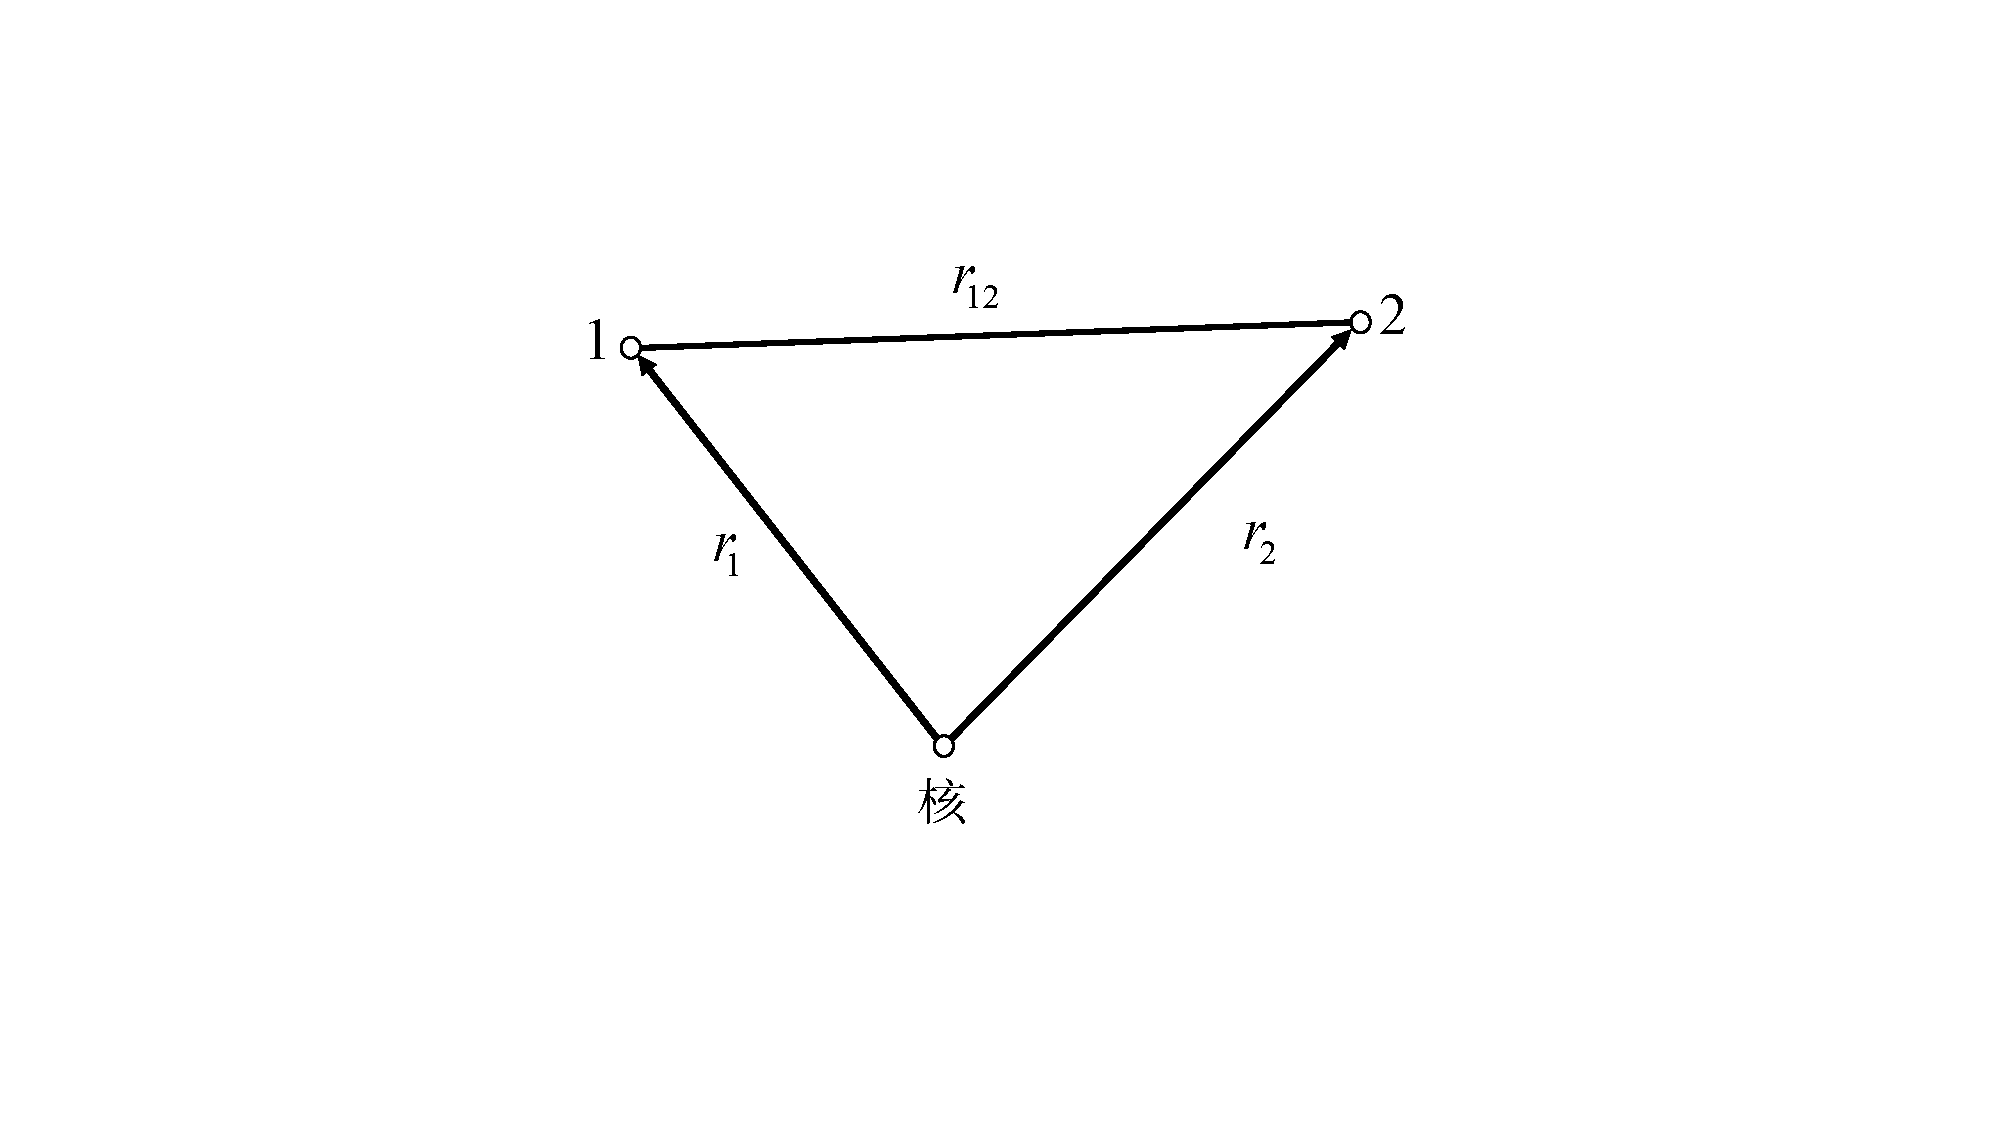
\includegraphics[width=3.5cm,clip]{QM file/figure/10-1}
	\caption{}\label{fig.10-1}
\end{wrapfigure}
这里略去了自旋-轨道耦合作用.


{\heiti 1. 正氦与仲氦}

体系的能级由定态薛定谔方程
\begin{empheq}{equation}\label{eqx3.2}
	H\Psi=E\Psi
\end{empheq}\eqllong
决定.由于$H$不含自旋变量,$\Psi$可以分离变量地表示成
\begin{equation}\label{eqx3.3}
	\Psi(q_{1},q_{2})=\varPsi(\boldsymbol{r}_{1},\boldsymbol{r}_{2})\chi(S_{1z},S_{2z})
\end{equation}\eqnormal
$\varPsi$为“轨道”波函数,$\chi$为自旋波函数.显然,$\varPsi$应该是$H$的本征函数,而$\chi$则与能级没有直接关系.

作为全同费密子体系的波函数,$\Psi$应该具有交换反对称性,即
\begin{empheq}{equation*}
	\hat{P}_{12}\Psi=(\hat{P}_{12}\varPsi)(\hat{P}_{12}\chi)=-\Psi=-\varPsi\chi
\end{empheq}\eqindent{1}
有两种可能的配合:
\begin{empheq}{align}
&(\si{i})	&&\hat{P}_{12}\varPsi=-\varPsi,\qquad \hat{P}_{12}\chi=\chi	\label{eqx3.4}\\
&(\si{ii})	&&\hat{P}_{12}\varPsi=\varPsi,\qquad \hat{P}_{12}\chi=-\chi	\label{eqx3.5}
\end{empheq}\eqnormal
第一种情形轨道波函数$\varPsi$是交换反对称的,自旋波函数则是交换对称的.第二种情形刚好相反.

二电子体系的自旋波函数共有4种(参看$\S$\ref{sec:07.08}),交换对称态有3种,即$\chi_{11},\chi_{10},\chi_{1-1}$,反对称态只有1种,即$\chi_{00}$.对称态相应于总自旋$S=1$,反对称态相应于$S=0$通常将氦原子按其自旋状态分类,称为正氦和仲氦:

正氦:$S=1,\chi=\chi_{11},\chi_{10},\chi_{1-1},\varPsi(\boldsymbol{r}_{1},\boldsymbol{r}_{2})$反对称

仲氦:$S=0,\chi=\chi_{00},\varPsi(\boldsymbol{r}_{1},\boldsymbol{r}_{2})$对称

\noindent 从表面上看,能级仅与$\varPsi(\boldsymbol{r}_{1},\boldsymbol{r}_{2})$有关,与$\chi$无直接关系.但因$\varPsi,\chi$的交换对称性互相制约,而$\varPsi$的交换对称性直接影响到体系的能量.[如$\varPsi$为反对称,$\varPsi(\boldsymbol{r}_{1},\boldsymbol{r}_{2})=-\varPsi(\boldsymbol{r}_{2},\boldsymbol{r}_{1})$,当$\boldsymbol{r}_{1}=\boldsymbol{r}_{2}$,$\varPsi=0$,因此两电子位置接近的概率较小,从而$\frac{\e^{2}}{r_{12}}$的平均值偏小.如$\varPsi$为交换对称,就没有这种性质.]所以正氦与仲氦将具有不同的能级.正氦的每一个能级都相应于自旋三重态,仲氦能级相应于自旋单态.

{\heiti 2. 微扰论} 

将两电子的相互作用势$\frac{\e^{2}}{r_{12}}$当作微扰,\eqref{eqx3.1}式可以表示成
\begin{empheq}{equation}\label{eqx3.6}
	H=H_{0}(\boldsymbol{r}_{1})+H_{0}(\boldsymbol{r}_{2})+H^{\prime}
\end{empheq}\eqlong
其中
\begin{empheq}{equation}\label{eqx3.7}
	H^{\prime}=\frac{\e^{2}}{r_{12}},\quad H_{0}(\boldsymbol{r}_{i})=-\frac{\hbar^{2}}{2m_{e}}\nabla_{i}^{2}-\frac{2\e^{2}}{r_{i}}\quad(i=1,2)
\end{empheq}\eqnormal
$H_{0}(\boldsymbol{r}_{i})$的本征值与本征函数就是类氢离子$(Z=2)$的能级与波函数
\begin{empheq}{equation}\label{eqx3.8}
	E_{n}=-\frac{4\e^{2}}{2n^{2}a_{0}},\quad \varPsi_{nlm}=R_{nl}Y_{lm}
\end{empheq}\eqlong
按照微扰论,轨道波函数的零级近似应该是$H_{0}(\boldsymbol{r}_{1})+H_{0}(\boldsymbol{r}_{2})$的本征函数,其一般形式为
\begin{empheq}{equation}\label{eqx3.9}
	\varPsi_{nlm}(\boldsymbol{r}_{1})\varPsi_{n^{\prime}l^{\prime}m^{\prime}}(\boldsymbol{r_{2}}),\quad \varPsi_{n^{\prime}l^{\prime}m^{\prime}}(\boldsymbol{r}_{1})\varPsi_{nlm}(\boldsymbol{r}_{2})
\end{empheq}\eqlllong
相应于能级(零级近似)$E_{n}+E_{n^{\prime}}$.在以下的叙述中,量子数$nlm$将简记成$n$.作为二电子体系的轨道波函数,应该具有交换对称或反对称性,显然应取下列形式:
\begin{empheq}{equation}\label{eqx3.10}
	\begin{aligned}
		\varPsi_{nn}^{S}(\boldsymbol{r}_{1},\boldsymbol{r}_{2}) &=\varPsi_{n}(\boldsymbol{r}_{1})\varPsi_{n}(\boldsymbol{r}_{2})	\\
		\varPsi_{nn^{\prime}}^{S}(\boldsymbol{r}_{1},\boldsymbol{r}_{2})	 &=\frac{1}{\sqrt{2}}[\varPsi_{n}(\boldsymbol{r}_{1})\varPsi_{n^{\prime}}(\boldsymbol{r_{2}})+\varPsi_{n^{\prime}}(\boldsymbol{r}_{1})\varPsi_{n}(\boldsymbol{r}_{2})]\quad (n\neq n^{\prime})		\\
		\varPsi_{nn^{\prime}}^{A}(\boldsymbol{r}_{1},\boldsymbol{r}_{2}) &=\frac{1}{\sqrt{2}}[\varPsi_{n}(\boldsymbol{r}_{1})\varPsi_{n^{\prime}}(\boldsymbol{r_{2}})-\varPsi_{n^{\prime}}(\boldsymbol{r}_{1})\varPsi_{n}(\boldsymbol{r}_{2})]\quad (n\neq n^{\prime})
	\end{aligned}
\end{empheq}\eqlong
由于微扰$H^{\prime}=\frac{\e^{2}}{r_{12}}$是交换对称的,必然有
\begin{empheq}{equation}\label{eqx3.11}
	\langle \varPsi^{S}|H^{\prime}|\varPsi^{A}\rangle=\iint\varPsi^{S*}\frac{\e^{2}}{r_{12}}\varPsi^{A}d\tau_{1}d\tau_{2}=0
\end{empheq}\eqnormal
(在上式中交换$\boldsymbol{r}_{1},\boldsymbol{r}_{2}$,相当于$\boldsymbol{r}_{1}$改写成$\boldsymbol{r}_{2}$,$\boldsymbol{r}_{2}$改写成$\boldsymbol{r}_{1}$,对于积分值显然没有影响.但这样做时,$\varPsi^{S}$,$\frac{\e^{2}}{r_{12}}$不变,$\varPsi^{A}$则要变号,因此积分值要变号.由此可知积分值必为.)按照简并化微扰论,既然微扰$H^{\prime}$并不造成对称态与反对称态间的耦合,能级的一级修正就等于$H^{\prime}$的平均值,记为
\begin{empheq}{equation}\label{eqx3.12}
	\begin{aligned}
		E_{nn}^{S} &= \langle \varPsi_{nn}^{S}|\frac{\e^{2}}{r_{12}}|\varPsi_{nn}^{S} \rangle 	\\
		E_{nn^{\prime}}^{S} &= \langle \varPsi_{nn^{\prime}}^{S}|\frac{\e^{2}}{r_{12}}|\varPsi_{nn^{\prime}}^{S} \rangle 	\\
		E_{nn^{\prime}}^{A} &= \langle \varPsi_{nn^{\prime}}^{S}|\frac{\e^{2}}{r_{12}}|\varPsi_{nn^{\prime}}^{A} \rangle 	
	\end{aligned}
\end{empheq}
显然
\begin{empheq}{align}\label{eqx3.13}
	E_{nn}^{S} &=\iint\frac{\e^{2}}{r_{12}}|\varPsi_{n}(\boldsymbol{r}_{1})|^{2}|\varPsi_{n}(\boldsymbol{r}_{2})|^{2}d\tau_{1}d\tau_{2}	\nonumber\\
	&\equiv C(n,n)
\end{empheq}
这是电子1,2均处于轨道态$\varPsi_{n}$时,它们之间的库仑作用势的平均值.对于\eqref{eqx3.12}式的后二式,可以算出
\begin{empheq}{align}
	E_{nn^{\prime}}^{S} &=C(n,n^{\prime})+J(n,n^{\prime})	\label{eqx3.14}\\
	E_{nn^{\prime}}^{A} &=C(n,n^{\prime})-J(n,n^{\prime})	\label{eqx3.15}
\end{empheq}\eqlong
其中
\begin{empheq}{align}
	C(n,n^{\prime}) &=\iint\frac{\e^{2}}{r_{12}}|\varPsi_{n}(\boldsymbol{r}_{1})|^{2}|\varPsi_{n^{\prime}}(\boldsymbol{r}_{2})|^{2}d\tau_{1}d\tau_{2}	\nonumber\\
	&=\iint\frac{\e^{2}}{r_{12}}|\varPsi_{n^{\prime}}(\boldsymbol{r}_{1})|^{2}|\varPsi_{n}(\boldsymbol{r}_{2})|^{2}d\tau_{1}d\tau_{2}		\label{eqx3.16}\\
	J(n,n^{\prime}) &=\iint\frac{\e^{2}}{r_{12}}\varPsi_{n}^{*}(\boldsymbol{r}_{1})\varPsi_{n^{\prime}}(\boldsymbol{r}_{1})\varPsi_{n^{\prime}}^{*}(\boldsymbol{r}_{2})\varPsi_{n}(\boldsymbol{r}_{2})d\tau_{1}d\tau_{2}	\label{eqx3.17}
\end{empheq}
习惯上称$C(n,n^{\prime})$为“库仑能”,称$J(n,n^{\prime})$为“交换能”,其实它们都是两电子间库仑作用势$\frac{\e^{2}}{r_{12}}$平均值的一部分.从形式上看,$C(n,n^{\prime})$相当于一个电子处于$\varPsi_{n}$态,另一个电子处于$\varPsi_{n^{\prime}}$态时$\frac{\e^{2}}{r_{12}}$的平均值.$J(n,n^{\prime})$则没有这样直观简单的解释,它是两个电子交换其单电子态的产物,根源在于波函数的交换对称性.

总结上述计算,准确到微扰论一级近似,氦原子能级为:

正氦($S=1$,$\varPsi$反对称)
\begin{empheq}{equation}\label{eqx3.18}
	E=E_{n}+E_{n^{\prime}}+C(n,n^{\prime})-J(n,n^{\prime})\quad (n\neq n^{\prime})
\end{empheq}

仲氦($S=0$,$\varPsi$对称)
\begin{empheq}{align}
	E&=2E_{n}+C(n,n)\quad (n=n^{\prime})		\label{eqx3.19}\\
	E&=E_{n}+E_{n^{\prime}}+C(n,n^{\prime})+J(n,n^{\prime})\quad (n\neq n^{\prime})	\label{eqx3.20}
\end{empheq}\eqnormal
$C(n,n^{\prime})$与$J(n,n^{\prime})$的计算相当繁,从略.当$n,n^{\prime}$较小时,$C$与$J$均为正,但$J(n,n^{\prime})<C(n,n^{\prime})$,所以当$n\neq n^{\prime}$,正氦和仲氦能级接近,仲氦稍高.但仲氦还有$n=n^{\prime}$(两个电子处于相同状态)的能级,即\eqref{eqx3.19}式.氦原子的低激发态,一个电子处于最低的$E_{1}$能级($\varPsi_{100}$态),另一个电子处于$E_{n}$能级($\varPsi_{nlm}$态,$n\geqslant2$),由于$\varPsi_{100}$与$\varPsi_{nlm}$重叠较少,因此交换能$J(100,nlm)$显得微不足道.只有当两个电子同处一个壳层($n$相同,$lm\neq l^{\prime}m^{\prime}$),空间位置较接近,交换能才变得重要.

{\heiti 3. 基态(微扰论及变分法)} 

氦原子的基态属于仲氦,两个电子同处轨道态$\varPsi_{100}$,总自旋为0.按照微扰论,轨道波函数(零级近似)为
\begin{empheq}{equation}\label{eqx3.21}
	\varPsi_{100,100}^{S}(r_{1},r_{2})=\varPsi_{100}(r_{1})\varPsi_{100}(r_{2})
\end{empheq}
其中$\varPsi_{100}$为类氢离子$(Z=2)$基态波函数,即
\begin{empheq}{equation}\label{eqx3.22}
	\varPsi_{100}(r)=\left(\frac{8}{\pi a_{0}^{3}}\right)^{\frac{1}{2}}e^{-2r/a_{0}}
\end{empheq}
利用公式
\begin{empheq}{equation}\label{eqx3.23}
	\iint\frac{1}{r_{12}}e^{-\alpha(r_{1}+r_{2})}d\tau_{1}d\tau_{2}=\frac{20\pi^{2}}{\alpha^{5}}\quad (\alpha>0)
\end{empheq}
(证明见本节末)容易算出
\begin{empheq}{equation}\label{eqx3.24}
	C(100,100)=\frac{5}{4}\cdot\frac{\e^{2}}{a_{0}}
\end{empheq}\eqlong
因此氦原子基态能量的微扰论结果为
\begin{empheq}{equation}\label{eqx3.25}
	E_{0}(\text{微扰论})=2E_{1}+C(100,100)=-\num{2.75}\frac{\e^{2}}{a_{0}}
\end{empheq}\eqnormal
实验值则是
\begin{empheq}{equation*}
	E_{0}(\text{实验})=-\num{79.01}\si{eV}=-\num{2.9037}\frac{\e^{2}}{a_{0}}
\end{empheq}
二者约相差5.3\%.

在上述微扰论计算中,电子的轨道波函数\eqref{eqx3.22}式描述的是电子在原子核所生库仑场中的运动,忽略了另一个电子的存在所产生的影明.事实上,另一个电子的存在,将在一定程度上对核电荷起屏蔽作用,每一个电子感受到的总库仑势(原子核及另一个电子的库仑势之和)粗略地等效于电荷$\lambda e(1<\lambda<2)$产生的库仑势如改用变分法计算,就可以反映这种屏蔽效应.取变分试探函数
\begin{empheq}{align}\label{eqx3.26}
	\varPsi(\lambda,r_{1},r_{2}) &=\varPsi(\lambda,r_{1})\varPsi(\lambda,r_{2})	\nonumber\\
	&=\frac{\lambda^{3}}{\pi a_{0}^{3}}e^{-\lambda r_{1}/a_{0}}e^{-\lambda r_{2}/a_{0}}
\end{empheq}
作为氦原子基态轨道波函数的近似,其中$\lambda$为变分参数.上式已经归一化.当$\lambda=2$,上式就是\eqref{eqx3.21}式.

对\eqref{eqx3.26}式计算总能量H的平均值,即
\begin{empheq}{equation*}
	E(\lambda)=\langle\varPsi(\lambda,r_{1},r_{2})|H|\varPsi(\lambda,r_{1},r_{2})\rangle 
\end{empheq}\eqlong
容易求得
\begin{empheq}{align}
	\langle\nabla_{1}^{2}\rangle =&\langle\nabla_{2}^{2}\rangle=\int\varPsi(\lambda,r)\nabla^{2}\varPsi(\lambda,r)d\tau	\nonumber\\
	=&-\int|\nabla\varPsi(\lambda,r)|^{2}d\tau=-\left(\frac{\lambda}{a_{0}}\right)-\nonumber \\
	&\frac{\hbar^{2}}{2m_{e}}\langle\nabla_{1}^{2}+\nabla_{2}^{2}\rangle=\frac{\hbar^{2}\lambda^{2}}{m_{e}a_{0}}=\lambda^{2}\frac{\e^{2}}{a_{0}} \label{eqx3.27}\\
	\left\langle\frac{1}{r_{1}}\right\rangle=&\left\langle\frac{1}{r_{2}}\right\rangle=\int\frac{1}{r}\varPsi^{2}(\lambda,r)d\tau=\frac{\lambda}{a_{0}}-\nonumber\\& 2\e^{2}\left\langle\frac{1}{r_{1}}+\frac{1}{r_{2}}\right\rangle=-4\lambda\frac{\e^{2}}{a_{0}}		\label{eqx3.28}\\
	\left\langle\frac{\e^{2}}{r_{12}}\right\rangle=&\e^{2}\iint\frac{1}{r_{12}}\varPsi^{2}(\lambda,r_{1})\varPsi^{2}(\lambda,r_{2})d\tau_{1}d\tau_{2}	\nonumber\\
	=&\frac{5\lambda}{8}\frac{\e^{2}}{a_{0}}		\label{eqx3.29}
\end{empheq}\eqnormal
因此
\begin{empheq}{equation}\label{eqx3.30}
	E(\lambda)=\left(\lambda^{2}-\frac{27}{8}\lambda\right)\frac{\e^{2}}{a_{0}}
\end{empheq}
由极值条件$\frac{\partial E(\lambda)}{\partial\lambda}$.求得$\lambda$的最佳值为$\lambda_{0}=\frac{27}{16}$.所以基态能级的变分法结果为
\begin{empheq}{equation}\label{eqx3.31}
	E(\lambda_{0})=-\left(\frac{27}{16}\right)^{2}\frac{\e^{2}}{a_{0}}=-\num{2.8477}\frac{\e^{2}}{a_{0}}
\end{empheq}
这结果比实验值略高,二者相差1.93\%.与微扰论结果相比,变分法结果已大有改进.如果试探波函数的构造再复杂一些,结果还可以改善,直到与实验值完全符合.由此可见,量子力学理论辅以恰当的数学方法,可以成功地处理原子构造问题.

\eqref{eqx3.23}式的证明如下.将积分写成
\begin{empheq}{equation*}
	I-\iint d\tau_{2}I_{1}e^{-\alpha r_{2}},\quad I_{1}=\int\frac{1}{r_{12}}e^{-\alpha r_{1}}d\tau_{1}
\end{empheq}
计算$I_{1}$时,取$\boldsymbol{r}_{2}$为极轴(参看图\ref{fig.10-2}),$\boldsymbol{r}_{1}$用球坐标,则
\begin{empheq}{align*}
	d\tau_{1}&=r_{1}^{2}dr_{1}\sin\theta d\theta d\varphi	\\
	r_{12}&=(r_{1}^{2}+r_{2}^{2}-2r_{1}r_{2}\cos\theta)^{\frac{1}{2}}
\end{empheq}\eqindent{3}
\begin{wrapfigure}[6]{r}{5em}
	\centering
	\small
	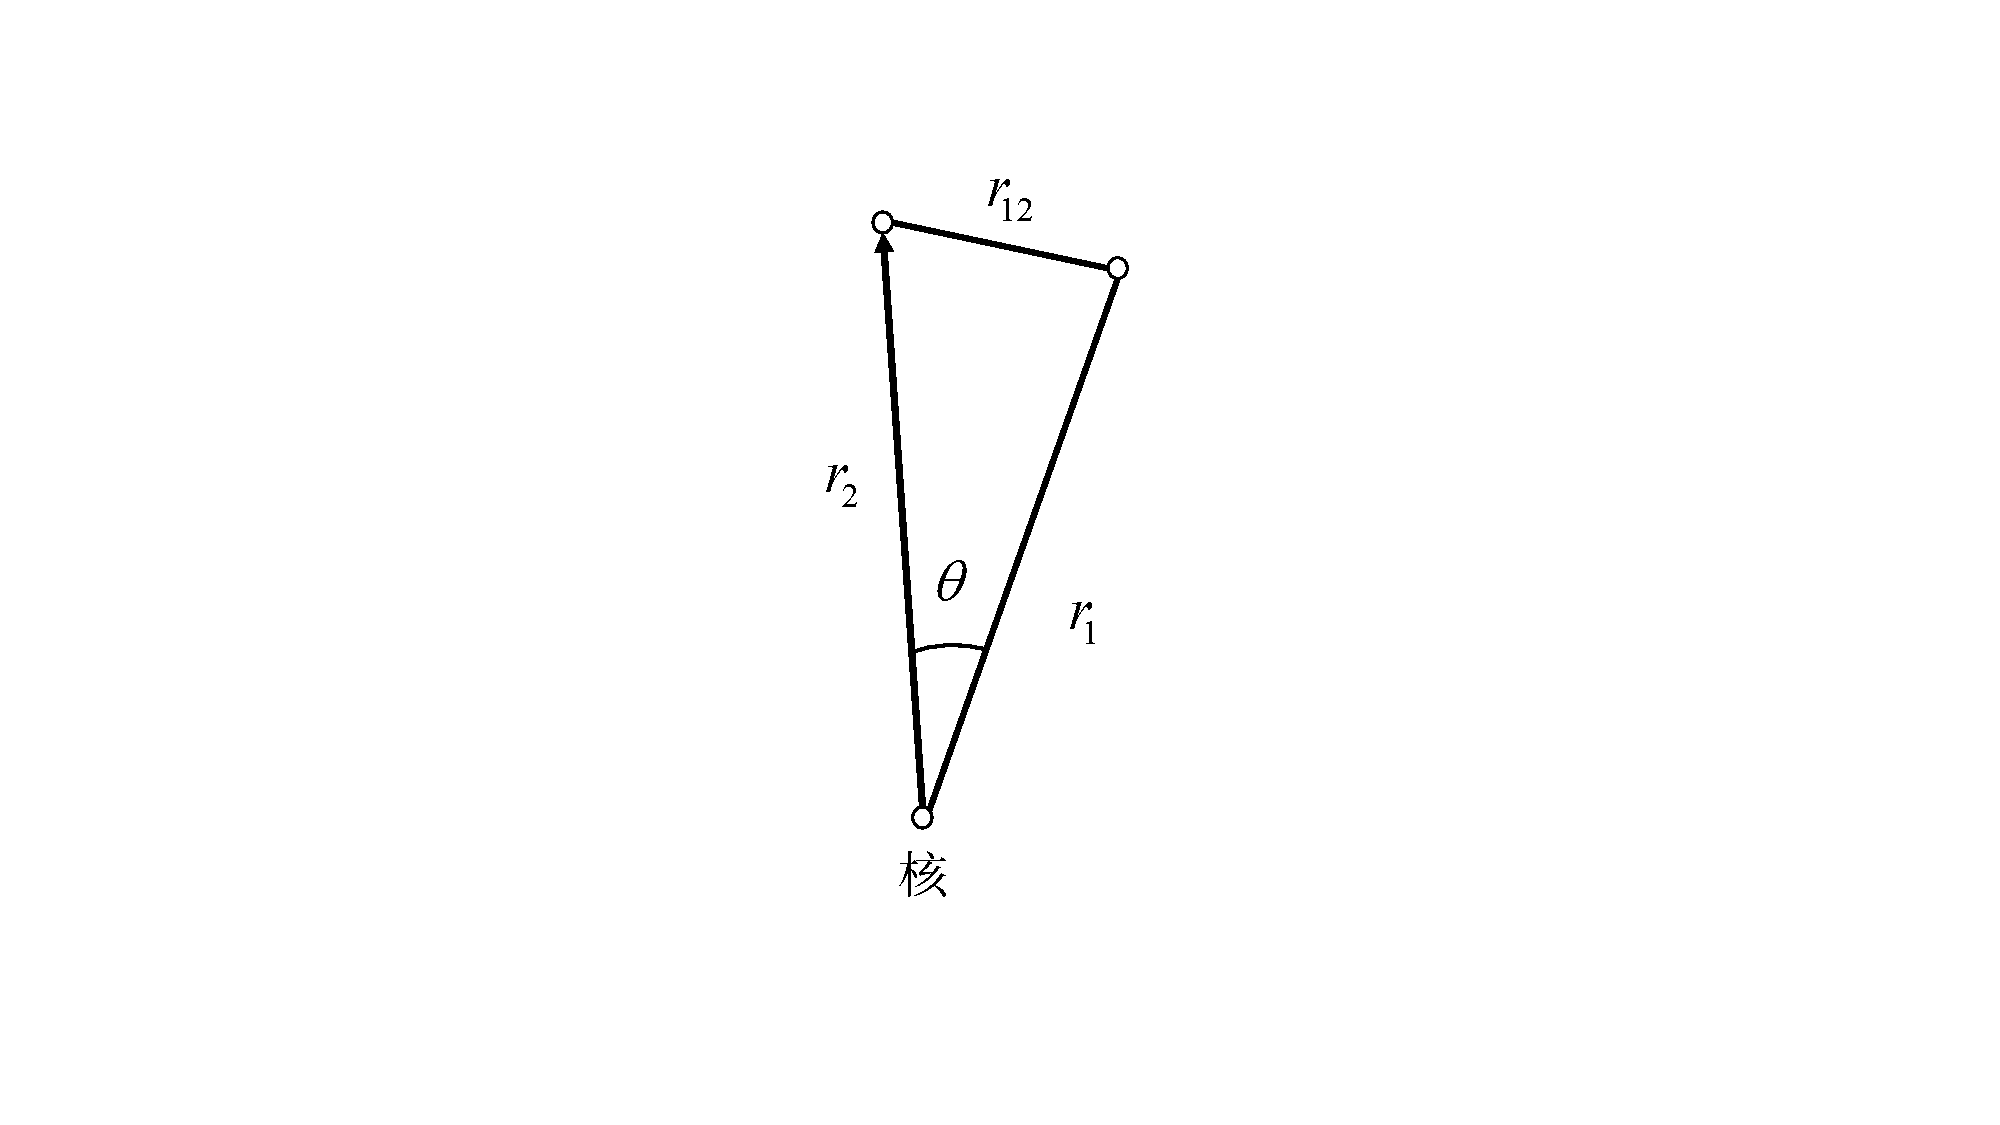
\includegraphics[width=2cm,clip]{QM file/figure/10-2}
	\caption{}\label{fig.10-2}
\end{wrapfigure}
容易算出
\begin{empheq}{equation*}
	I_{1}=\int_{0}^{\infty}dr_{1}r_{1}^{2}e^{-\alpha r_{1}}2\pi\int_{0}^{\pi}(r_{1}^{2}+r_{2}^{2}-2r_{1}r_{2}\cos\theta)^{\frac{1}{2}}\sin\theta d\theta
\end{empheq}\eqlong
其中
\begin{empheq}{align*}
	&\int_{0}^{\pi}(r_{1}^{2}+r_{2}^{2}-2r_{1}r_{2}\cos\theta)^{\frac{1}{2}}\sin\theta d\theta	\\
	=&\frac{1}{r_{1}r_{2}}(r_{1}^{2}+r_{2}^{2}-2r_{1}r_{2}\cos\theta)^{\frac{1}{2}}\bigg|_{\theta=0}^{\theta=\pi} \\
	=&\frac{1}{r_{1}r_{2}}[(r_{1}+r_{2})-|r_{1}-r_{2}|]	\\
	=&\begin{dcases}
		\frac{2}{r_{2}},\quad r_{1}<r_{2}	\\
		\frac{2}{r_{1}},\quad r_{1}>r_{2}
	\end{dcases}	
\end{empheq}
因此
\begin{empheq}{align*}
	I_{1}=&4\pi\int_{0}^{r_{2}}\frac{1}{r_{2}}r_{1}^{2}e^{-\alpha r_{1}}dr_{1}+4\pi\int_{r_{2}}^{\infty}r_{1}e^{-\alpha r_{1}}dr_{1}	\\
	&=\frac{4\pi}{\alpha^{2}}\left[ \frac{2}{\alpha r_{2}}-\left(1+\frac{2}{\alpha r_{2}}\right)e^{-\alpha r_{2}} \right]
\end{empheq}
代入$I$中,即得
\begin{empheq}{align*}
	I&=r\pi\int_{0}^{\infty}I_{1}e^{-\alpha r_{2}}r_{2}^{2}dr_{2}	\\
	&=\frac{16\pi^{2}}{\alpha^{5}}\int_{0}^{\infty}x^{2}e^{-x}\left[\frac{2}{x}-\left(1+\frac{2}{x}\right)e^{-x} \right]	\\
	&=20\pi^{2}/\alpha^{5}
\end{empheq}\eqnormal
此即\eqref{eqx3.23}式.





% 氢分子
\section[氢分子]{氢分子} \label{sec:10.04} % 
% \makebox[5em][s]{} % 短题目拉间距

1927年,Heitler-London用量子力学方法研究氢分子结构获得成功,开创了量子化学.

氢分子包含两个原子核$(a,b)$及两个电子$(1,2)$,如图\ref{fig.10-3} 所示.如略去原子核的运动(即分子的振动、转动和平移),就可以将氢分子当作二电子体系,体系的总能量算符可以表示成
\eqllong
\begin{empheq}{align}\label{eqx4.1}
	H=&-\frac{\hbar^{2}}{2m_{e}}(\nabla_{1}^{2}+\nabla_{2}^{2})-\e^{2}(\frac{1}{r_{1a}}+\frac{1}{r_{1b}}+\frac{1}{r_{2a}}+\frac{1}{r_{2b}})+ \nonumber\\
	&\frac{\e^{2}}{r_{12}}+\frac{\e^{2}}{R}
\end{empheq}
\begin{wrapfigure}[7]{r}{8em}
	\centering
	\small
	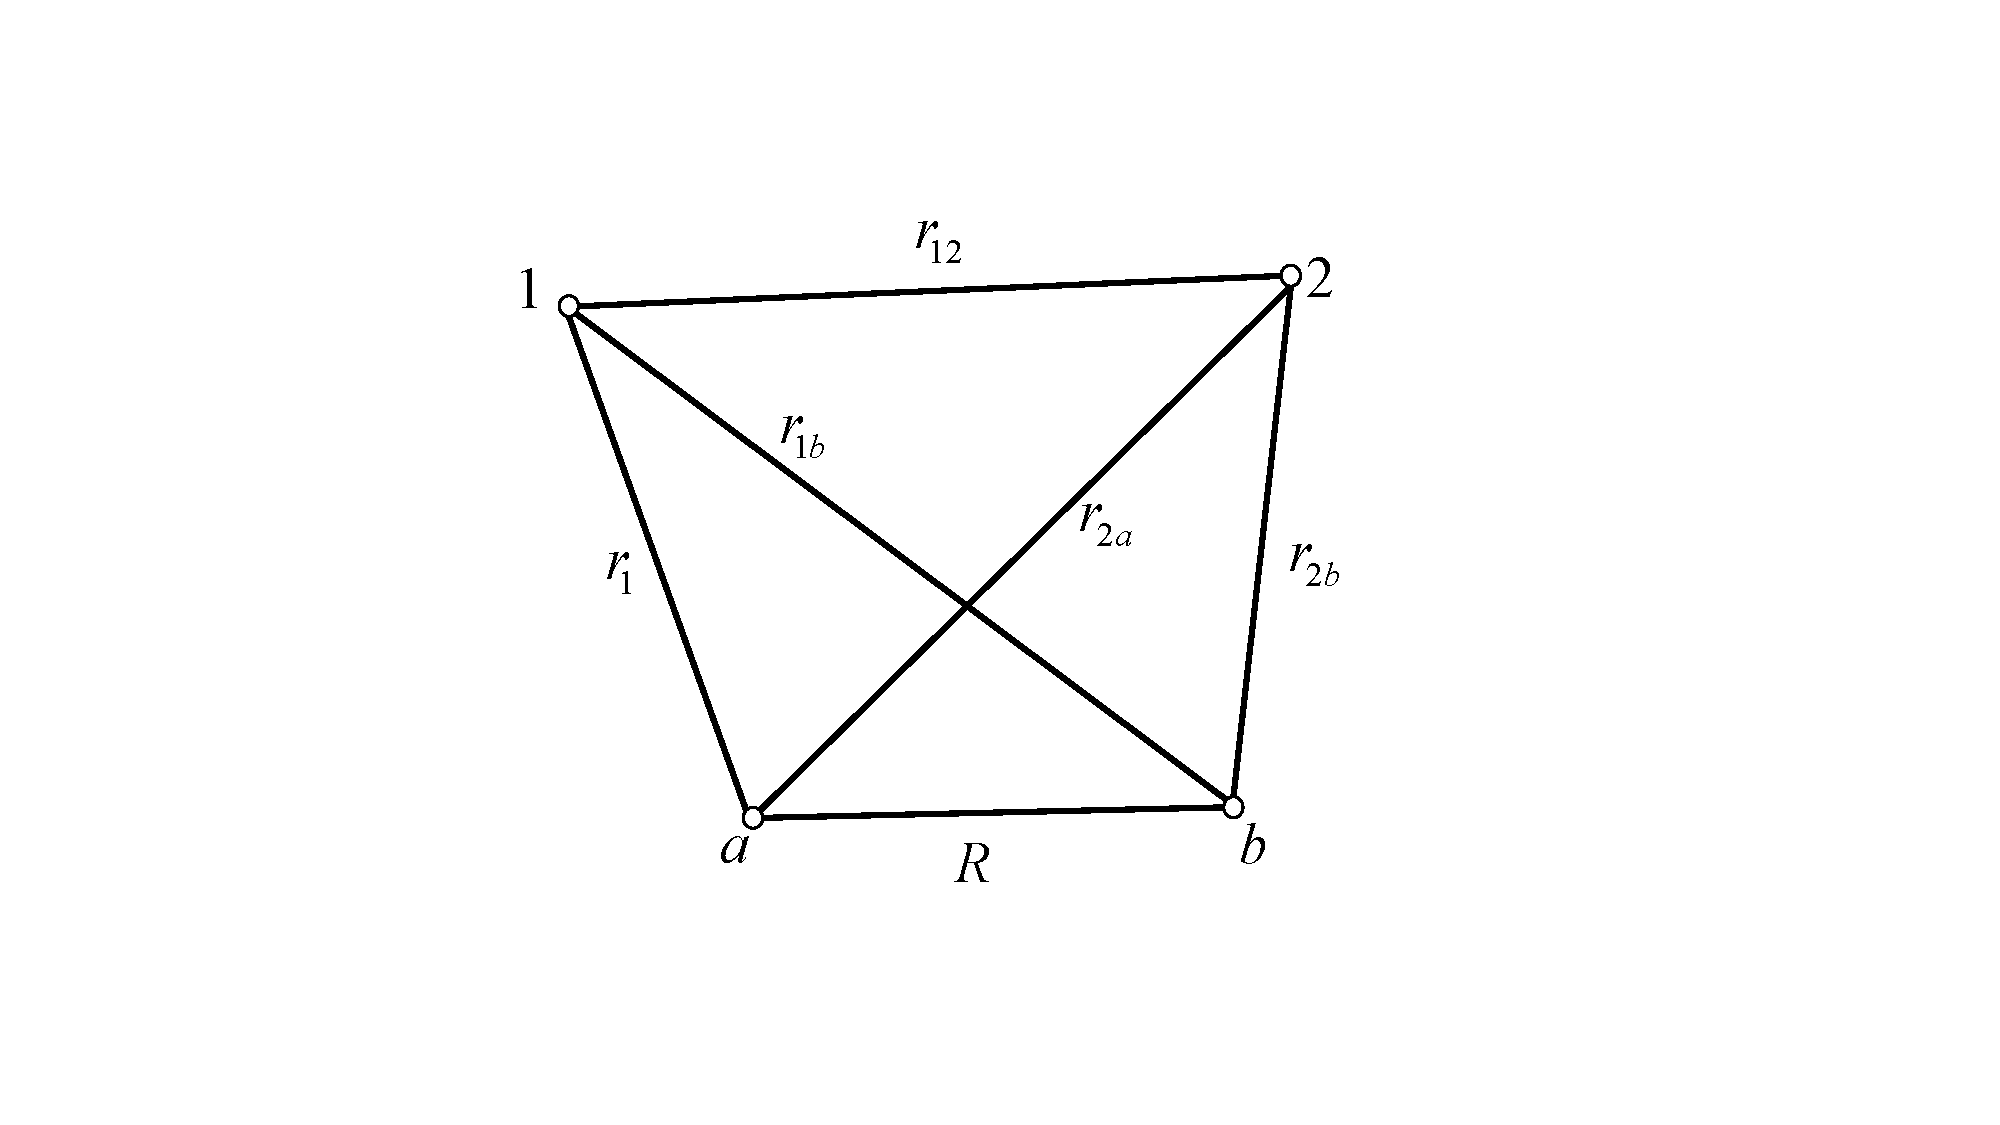
\includegraphics[width=3cm,clip]{QM file/figure/10-3}
	\caption{}\label{fig.10-3}
\end{wrapfigure}
其中共包含6项库仑作用势,最后一项是原子核$a,b$间的库仑能,它是分子能量的一部分,所以应包含在$H$中.在计算中$R$作为参量处理.

和氦原子相仿,二电子体系总波函数可以表示成轨道波函数与自旋波函数的积,
\begin{empheq}{equation}\label{eqx4.2}
	\Psi(q_{1},q_{2})=\varPsi(\boldsymbol{r}_{1},\boldsymbol{r}_{2})\chi(S_{1z},S_{2z})
\end{empheq}\eqnormal
$\varPsi$应满足能量本征方程
\begin{empheq}{equation}\label{eqx4.3}
	H\varPsi(\boldsymbol{r}_{1},\boldsymbol{r}_{2})=E\varPsi(\boldsymbol{r}_{1},\boldsymbol{r}_{2})
\end{empheq}
关于$\varPsi$及$\chi$的交换对称性的讨论以及结论,和氦原子相同,不再重述.由于有两个原子核(即两个库仑力中心),数学处理显然比氦原子更为困难.近似方法通常与物理模型结合使用,大致可分两类,即分子轨函法和原子轨函法.所谓分子轨道是指在原子核$a,b$的库仑场的共同作用下形成的单电子状态,也就是氢分子离子$(\ce{H_{2}^{+}})$的电子轨道态.氢分子的两个电子都处于分子轨道的基态.(自旋态$\chi_{00},S=0$电子间库仑作用$\frac{\e^{2}}{r_{12}}$则作为微扰处理.至于分子轨道波函数的确定仍然要用近似方法(两个库仑力中心!)所谓原子轨道是指孤立原子的单电子状态$\varPsi_{nlm}$.以此作为基础,设法计算两个原子的相互作用能.Heitler-London方法就是原子轨函法,这种方法计算方便,但是精确程度不如分子轨函法.本节只介绍原子轨函法.

考虑分子的形成过程如下:两个孤立的原子逐渐靠近,由于相互作用(电荷间的库仑作用)而结合成分子.以两个原子波函数的积作为分子波函数的零级近似,两原子的相互作用当作微扰.电子与原子核的配对有两种可能,(以每个原子核拥有一个电子为前提,相当于共价键;如二电子同属于一个原子核,就形成离子键.氢分子基本上是共价键类型)如图\ref{fig.10-4}所示,图左相当于原子$(a,2)$与$(b,1)$结合成分子,图右相当于原子$(a,2)$与$(b,1)$结合成分子,两种情形的轨道波函数分别为
\begin{figure}[!h]
	\centering
	\small
	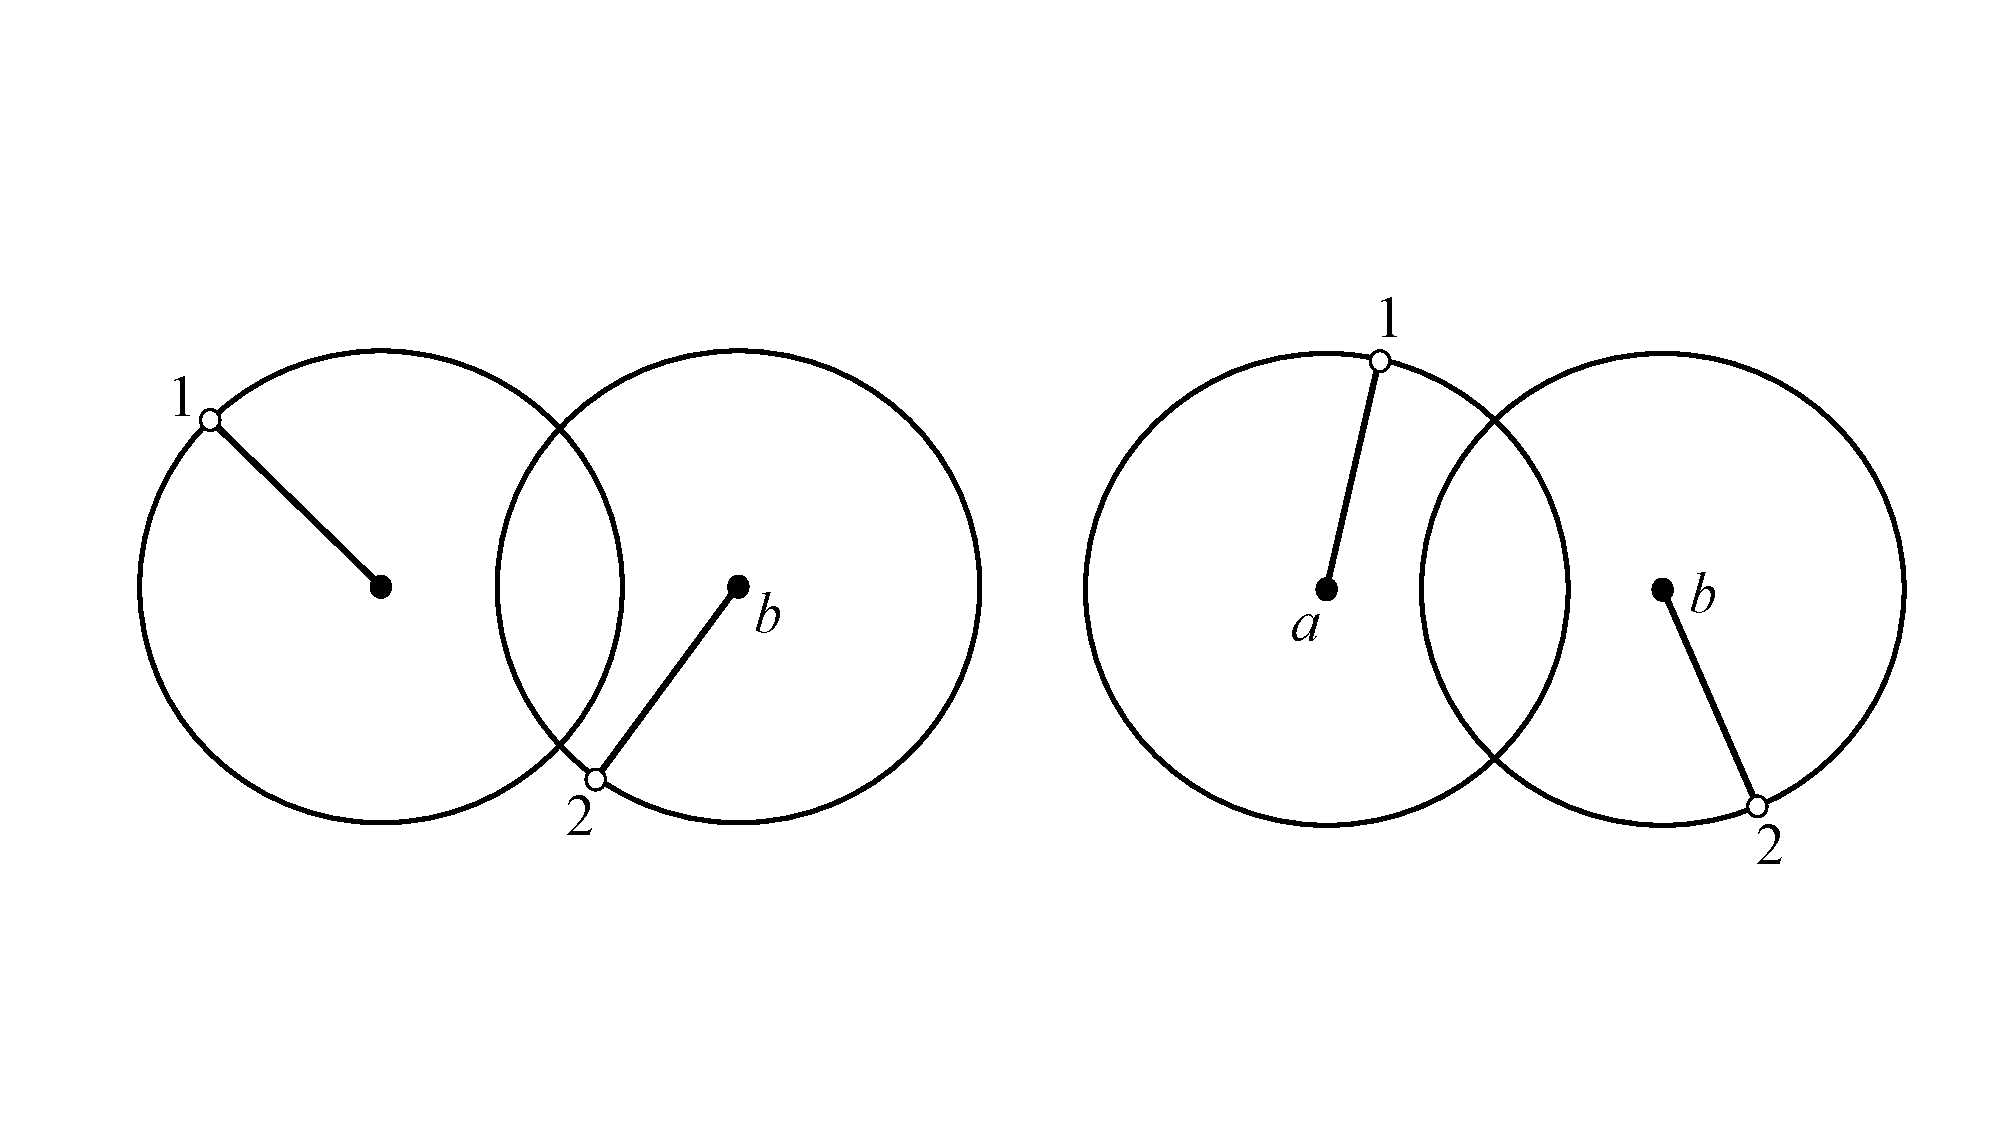
\includegraphics[width=7cm,clip]{QM file/figure/10-4}
	\caption{}\label{fig.10-4}
\end{figure}
\begin{empheq}{equation}\label{eqx4.4}
	\varPsi_{a}(1)\varPsi_{b}(2),\quad \varPsi_{a}(2)\varPsi_{b}(1)
\end{empheq}
其中$\varPsi_{a}(1)$指氢原子$(a,1)$的基态波函数,即
\begin{empheq}{equation}\label{eqx4.5}
	\varPsi_{a}(1)=\varPsi_{100}(r_{1a})=\left(\frac{1}{\pi a_{0}^{3}}\right)^{\frac{1}{2}}e^{-r_{1a}/a_{0}}
\end{empheq}
依此类推.将总能$H$分成$H_{0}$和$H^{\prime}$,$H_{0}$是与两个氢原子的构成有关的算符,$H^{\prime}$是两个原子的相互作用能.对于\eqref{eqx4.4}式中第一个波函数$\varPsi_{a}(1)\varPsi_{b}(2)$,$H_{0}$与$H^{\prime}$分别是
\begin{empheq}{equation}\label{eqx4.6}
	\begin{aligned}
		H_{0} &=-\frac{\hbar^{2}}{2m_{e}}(\nabla_{1}^{2}+\nabla_{2}^{2})-\frac{\e^{2}}{r_{1a}}-\frac{\e^{2}}{r_{1b}}	\\
		H^{\prime} &=\frac{\e^{2}}{R}+\frac{\e^{2}}{r_{12}}-\frac{\e^{2}}{r_{1b}}-\frac{\e^{2}}{r_{2a}}
	\end{aligned}
\end{empheq}
显然
\begin{empheq}{equation*}
	H_{0}\varPsi_{a}(1)\varPsi_{b}(2)=2E_{1}\varPsi_{a}(1)\varPsi_{b}(2),\quad E_{1}=-\frac{\e^{2}}{2a_{0}}
\end{empheq}
$E_{k}$是氢原子基态能级.对于\eqref{eqx4.4}式中第二个波函数$\varPsi_{a}(2)\varPsi_{a}(1)$,$H_{0}$与$H^{\prime}$应取
\begin{empheq}{equation*}\label{eqx4.6'}
	\begin{aligned}
		H_{0} &=-\frac{\hbar^{2}}{2m_{e}}(\nabla_{1}^{2}+\nabla_{2}^{2})-\frac{\e^{2}}{r_{1b}}-\frac{\e^{2}}{r_{2a}}	\\
		H^{\prime} &=\frac{\e^{2}}{R}+\frac{\e^{2}}{r_{12}}-\frac{\e^{2}}{r_{1a}}-\frac{\e^{2}}{r_{2b}}
	\end{aligned}\tag{$10.4.6^{\prime}$}
\end{empheq}
显然
\begin{empheq}{equation*}
	H_{0}\varPsi_{a}(2)\varPsi_{b}(1)=2E_{1}\varPsi_{a}(2)\varPsi_{b}(1)
\end{empheq}\eqlong

如果不管波函数的交换对称性,简单地以\eqref{eqx4.4}式中任何一个(例如第一个)波函数$\varPsi_{a}(1)\varPsi_{b}(2)$作为分子的近似波函数,而以$H^{\prime}$平均值当作分子的结合能,记为$W$,则
\begin{empheq}{equation}\label{eqx4.7}
	W=\iint\varPsi_{a}^{2}(1)\varPsi_{b}^{2}\left(\frac{\e^{2}}{R}+\frac{\e^{2}}{r_{12}}-\frac{\e^{2}}{r_{1b}}-\frac{\e^{2}}{r_{2a}}\right)e^{-2R/a_{0}}
\end{empheq}
$W$之值显然与$R$有关,计算结果为
\begin{empheq}{equation}\label{eqx4.8}
	W=\frac{\e^{2}}{a_{0}}\left(\frac{a_{0}}{R}+\frac{5}{8}-\frac{3}{4}\frac{R}{a_{0}}-\frac{1}{6}\frac{R^{2}}{a_{0}^{2}}\right)e^{-2R/a_{0}}
\end{empheq}
当$R=1.87 a_{0}$时$W$取极小值,
\begin{empheq}{equation}\label{eqx4.9}
	W(R=1.87 a_{0})=-\num{0.0196}\left(\frac{\e^{2}}{a_{0}}\right)=-\num{0.533}\si{eV}.
\end{empheq}\eqnormal
而氢分子结合能的实验值是\num{-4.72}\si{eV},键长$R=\num{0.07395}\si{nm}$.\eqref{eqx4.9}式与实验值相差太多,量级不符合,由此可见,如不考虑波函数的交换对称性,就不能解释氢分子的形成.

考虑到交换对称性,氢分子轨道波函数(零级近似)应取\eqref{eqx4.4}式中两项的对称或反对称组合.以$\varPsi_{ab}^{S}(\boldsymbol{r}_{1},\boldsymbol{r}_{2})$和$\varPsi_{ab}^{A}(\boldsymbol{r}_{1},\boldsymbol{r}_{2})$表示对称和反对称轨道波函数,它们是
\begin{empheq}{align}
	\varPsi_{ab}^{S} &=C_{S}[\varPsi_{a}(1)\varPsi_{b}(2)+\varPsi_{a}(2)\varPsi_{b}(1)]	\label{eqx4.10}\\
	\varPsi_{ab}^{A} &=C_{A}[\varPsi_{a}(1)\varPsi_{b}(2)-\varPsi_{a}(2)\varPsi_{b}(1)]	\label{eqx4.11}
\end{empheq}
$C_{S}$及$C_{A}$是归一化常数.由于叠加的两个波函数并不正交,$C_{S}$及$C_{A}$均不等于$\frac{1}{\sqrt{2}}$.原子轨道波函数$\varPsi_{a}(1)$等已经归一化.定义重叠积分
\begin{empheq}{align}\label{eqx4.12}
	D 	&=\int\varPsi_{a}(1)\varPsi_{b}(1)d\tau_{1}	\nonumber\\
		&=\frac{1}{\pi a_{0}^{3}}\int e^{-(r_{1a}+r_{1b})/a_{0}}d\tau_{1}	\nonumber\\
		&=\left(1+\frac{R}{a_{0}}+\frac{1}{3}\frac{R^{2}}{a_{0}^{2}}\right)e^{-R/a_{0}}
\end{empheq}
则
\begin{empheq}{equation}\label{eqx4.13}
	C_{S}^{2}=\frac{1}{2+2D^{2}},\quad C_{A}^{2}=\frac{1}{2-2D^{2}}
\end{empheq}
当$R\rightarrow0$,原子核$a,b$重合,$\varPsi_{a}=\varPsi_{b}$,$D\rightarrow1$.当$R\rightarrow\infty$,$\varPsi_{a}$与$\varPsi_{b}$完全不重叠,$D\rightarrow0$.用本节所述方法处理氢分子构造,所得键长$R=\num{0.08}\si{nm}=\num{1.518}a_{0},D=\num{0.72},D^{2}=\num{0.52}$.

对于\eqref{eqx4.10}、\eqref{eqx4.11}式分别计算$H^{\prime}$平均值,分别记为$V_{ab}^{S},V_{ab}^{A}$,则可算出
\begin{empheq}{align}
	V_{ab}^{S} &=\iint\varPsi_{ab}^{S}H^{\prime}\varPsi_{ab}^{S}d\tau_{1}d\tau_{2}	\nonumber\\
	&=\frac{W+J}{1+D^{2}}	\label{eqx4.14}\\
	V_{ab}^{A} &=\iint\varPsi_{ab}^{A}H^{\prime}\varPsi_{ab}^{A}d\tau_{1}d\tau_{2}	\nonumber\\
	&=\frac{W-J}{1-D^{2}}		\label{eqx4.15}
\end{empheq}\eqindent{1}
计算时$H^{\prime}$应视作用的对象而取\eqref{eqx4.6}式或\eqref{eqx4.6'}式.$W$由\eqref{eqx4.8}式表示,$J$由下式表示,
\begin{empheq}{align}\label{eqx4.16}
	J	&=\iint\varPsi_{a}(1)\varPsi_{b}(2)\left(\frac{\e^{2}}{R}+\frac{\e^{2}}{r_{12}}-\frac{\e^{2}}{r_{1a}}-\frac{\e^{2}}{r_{2b}}\right)\varPsi_{a}(2)\varPsi_{b}(1)d\tau_{1}d\tau_{2}	\nonumber\\
	&=\varPsi_{a}(2)\varPsi_{b}(1)\left(\frac{\e^{2}}{R}+\frac{\e^{2}}{r_{12}}-\frac{\e^{2}}{r_{1b}}-\frac{\e^{2}}{r_{2a}}\right)\varPsi_{a}(1)\varPsi_{b}(2)d\tau_{1}d\tau_{2}	
\end{empheq}\eqnormal
$W$的意义是两个电子各自占有确定的原子轨道时两个原子间的库仑作用平均值,通常称为库仑能.$J$的意义则是“交换能”,它仍来自两原子间的库仑作用,是电子波函数交换对称性的产物.$J$的计算相当复杂,结果无法用初等解析函数表示.数值计算表明,$V_{ab}^{S}$与$V_{ab}^{A}$都是$R$的函数,$V_{ab}^{S}$在$R=\num{1.518}a_{0}$处有极小值,$W$与$J$均为负值,但$|J|\gg|W|$,数值为
\begin{empheq}{equation*}
	V_{ab}^{S}=\frac{W+J}{1+D^{2}}=-\num{0.125}\left(\frac{\e^{2}}{a_{0}}\right)=-3.41\si{eV}
\end{empheq}
与氢分子结合能实验值$(-4.72\si{eV})$量级符合.由此可知,波函数的交换对称性及“交换能”对于氢分子的形成起了关键作用.其他的共价键分子,也是这样.总之,共价键分子的形成是与全同性原理有关的一种典型量子力学效应,不可能在经典物理或玻尔量子论的基础上予以解释.

由于$|J|\gg|W|,J<0$,所以$V_{ab}^{A}>0$,亦即\eqref{eqx4.11}式所描述的反对称轨道态不能使两原子结合成分子.氢分子的轨道状态近似地由\eqref{eqx4.10}式表示,它是对称态与此相关,氢分子中两个电子的自旋态必为反对称态$\chi_{00}$,总自旋$S=0$,这一点与实验结果完全一致.

$W,V_{ab}^{S},V_{ab}^{A}$随$R$的变化示意图如图\ref{fig.10-5}所示.

\begin{figure}[!h]
	\centering
	\small
	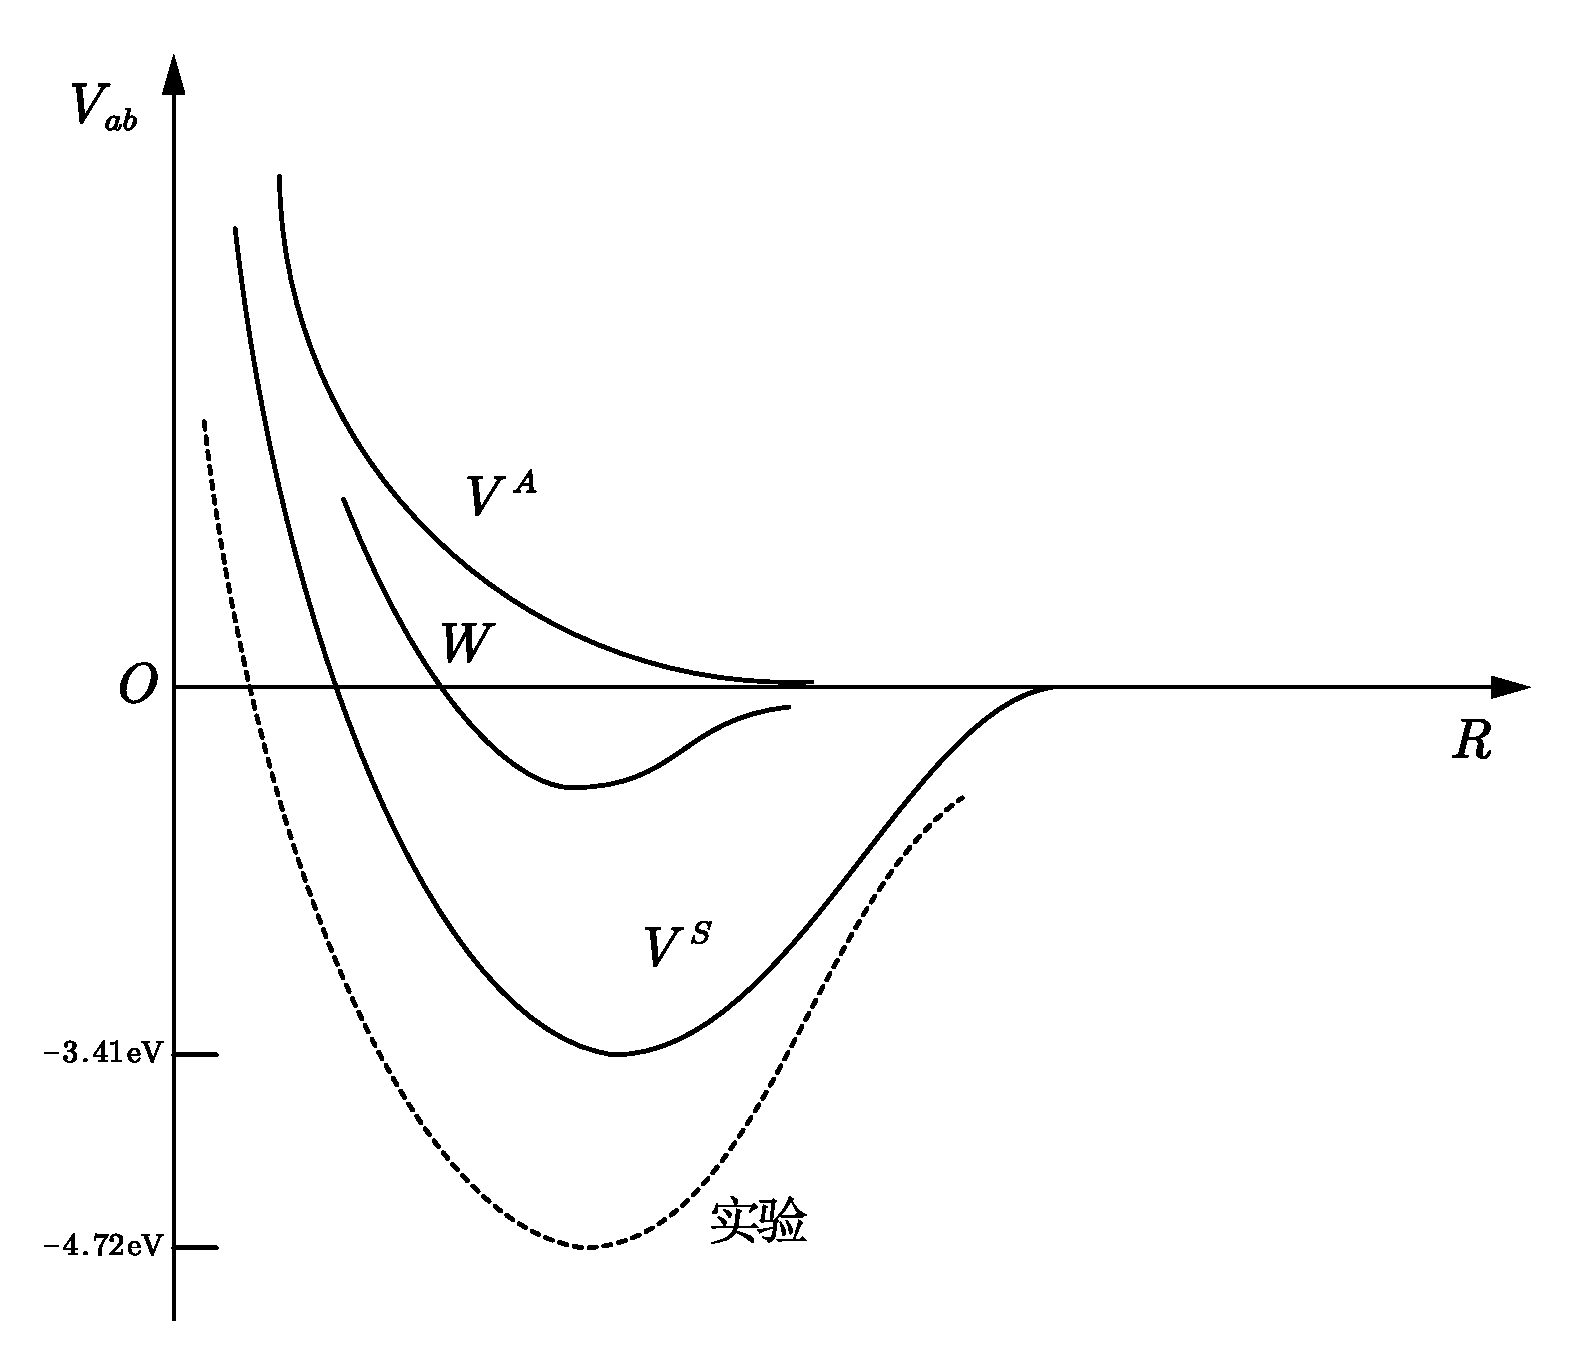
\includegraphics[width=5.5cm,clip]{QM file/figure/10-5}
	\caption{}\label{fig.10-5}
\end{figure}
\begin{wrapfigure}[7]{r}{7em}
	\centering
	\small
	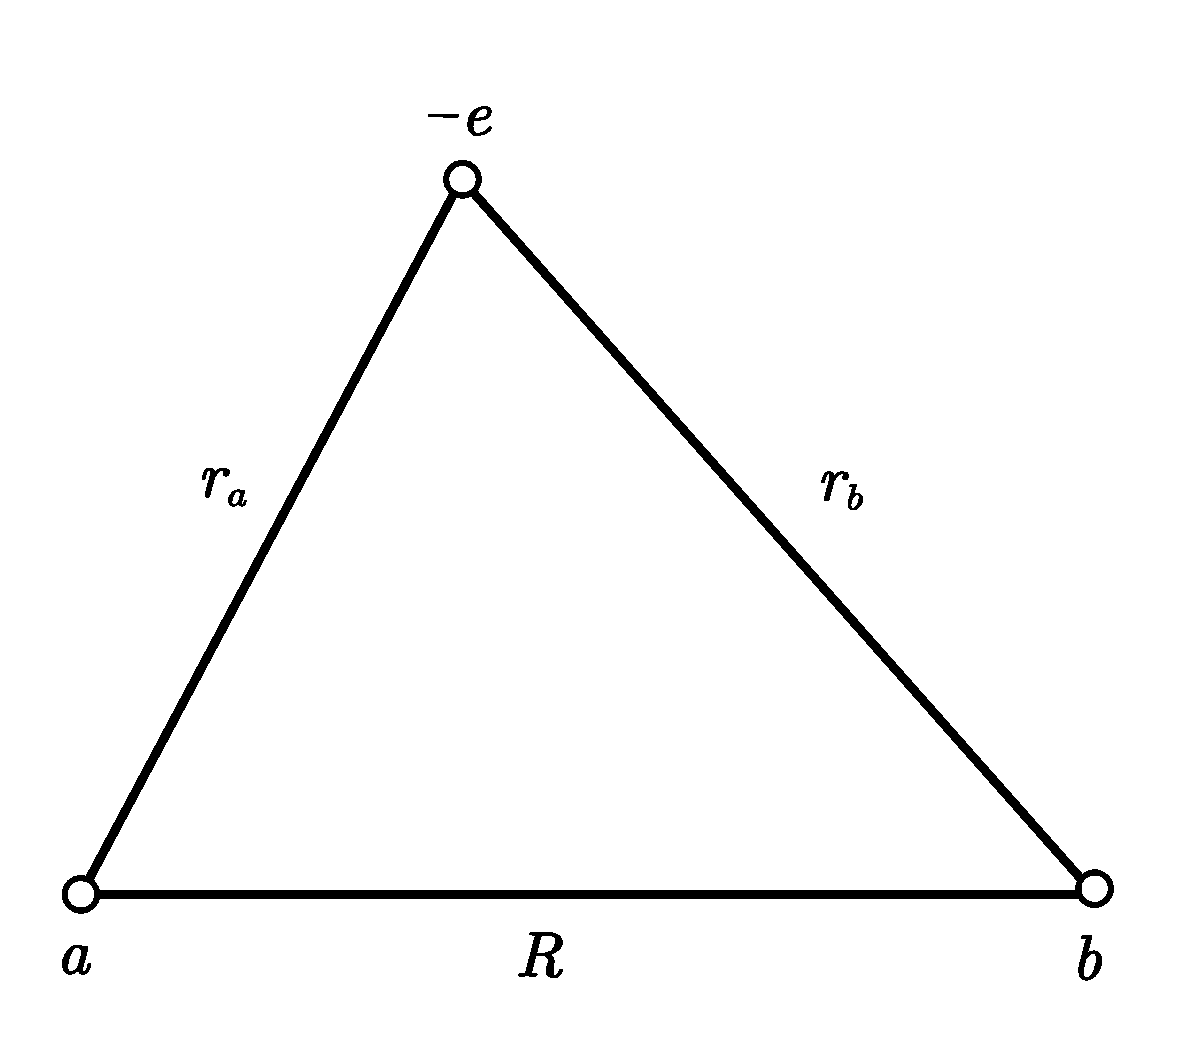
\includegraphics[width=3cm,clip]{QM file/figure/10-6}
	\caption{}\label{fig.10-6}
\end{wrapfigure}
詹姆斯等在考虑交换对称性的前提下,用变分法计算氢分子结合能.他们采用十分复杂的(包含13个变分参数)试探波函数,终于算出与实验值完全一致的结合能.

这表明分子的构造完全受量子力学规律支配,并没有任何超物理的因素起作用.

附录:重叠积分$D$和“库仑能”$W$的计算.

重叠积分$D$的定义见\eqref{eqx4.12}式,略去下标1,$D$可以写成
\begin{empheq}{equation*}
	D=\frac{1}{\pi a_{0}^{3}}\int e^{-(r_{a}+r_{b})/a_{0}}d\tau
\end{empheq}
$r_{a}$及$r_{b}$为电子至核$a$及核$b$之距离,如图10-6所示.引入共焦椭球坐标$(\xi,\eta,\varphi)$,定义为:
\begin{empheq}{align}\label{eqx4.17}
	\xi &=\frac{1}{R}(r_{a}+r_{b}),\quad 1\leqslant\xi <\infty	\\
	\eta&=\frac{1}{R}(r_{a}-r_{b}),\quad -1\leqslant\eta\leqslant1	\nonumber\\
	\varphi&\text{为绕ab轴的旋转角},0\leqslant\varphi <2\pi	\nonumber
\end{empheq}
体积元$d\tau$可以表示成
\begin{empheq}{equation}\label{eqx4.18}
	d\tau=\frac{R^{3}}{8}(\xi^{2}-\eta^{2})d\xi d\eta d\varphi
\end{empheq}
$r_{a},r_{b}$可以表示成
\begin{empheq}{equation}\label{eqx4.19}
	r_{a}=\frac{R}{2}(\xi+\eta),\quad r_{b}=\frac{R}{2}(\xi-\eta)
\end{empheq}\eqindent{5}
代入$D$中,即可算出
\begin{empheq}{align}\label{eqx4.20}
	D 
	&=\frac{1}{8\pi}\left(\frac{R}{a_{0}}\right)^{3}\int_{0}^{2\pi}d\varphi\int_{1}^{\infty}d\xi\int_{-1}^{1}d\eta(\xi^{2}-\eta^{2})e^{-\xi R/a_{0}}	\nonumber\\
	&=\frac{1}{4}\left(\frac{R}{a_{0}}\right)^{3}\int_{1}^{\infty}(2\xi^{2}-\frac{2}{3})e^{-\xi R/a_{0}}d\xi	\nonumber\\
	&=\left(1+\frac{R}{a_{0}}+\frac{1}{3}\frac{R^{2}}{a_{0}^{2}}\right)e^{-R/a_{0}}=D(R,a_{0})
\end{empheq}\eqnormal
此即\eqref{eqx4.12}式.积分的最后一步可用分部积分法算出.

“库仑能”$W$的定义见\eqref{eqx4.7}式.由于$\varPsi_{a}(1),\varPsi_{b}(2$均已归一化,显然
\begin{empheq}{equation*}
	\iint\varPsi_{a}^{2}(1)\varPsi_{b}^{2}(2)\frac{\e^{2}}{R}d\tau_{1}d\tau_{2}=\frac{\e^{2}}{R}
\end{empheq}\eqindent{5}
\begin{empheq}{align}\label{eqx4.21}
	&\iint\varPsi_{a}^{2}(1)\varPsi_{b}^{2}(2)\frac{1}{r_{1b}}d\tau_{1}d\tau_{2}
	=\iint\varPsi_{a}^{2}(1)\varPsi_{b}^{2}(2)\frac{1}{r_{2a}}d\tau_{1}d\tau_{2}	\nonumber\\
	&=\int\varPsi_{b}^{2}(2)\frac{1}{r_{2a}}d\tau_{2}=\frac{1}{\pi a_{0}^{3}}\int\frac{1}{r_{a}}e^{-2r_{b}/a_{0}}d\tau	\nonumber\\
	&=\frac{R^{3}}{4\pi a_{0}^{3}}\iiint d\xi d\eta d\varphi(\xi-\eta)e^{-(\xi-\eta)R/a_{0}}	\nonumber\\
	&=\frac{1}{R}-\left(\frac{1}{R}+\frac{1}{a_{0}}\right)e^{-2R/a_{0}}=I_{1}
\end{empheq}\eqnormal
\eqref{eqx4.7}式中较难的积分是
\begin{empheq}{equation}\label{eqx4.22}
	I_{2}=\iint\varPsi_{a}^{2}(1)\varPsi_{b}^{2}(2)\frac{1}{r_{12}}d\tau_{1}d\tau_{2}
\end{empheq}
先对d$\tau_{1}$积分,用普通球坐标,以原子核$a$作为坐标原点,对角度的积分仿照$\S$\ref{sec:10.03}曾用过的方法,$\frac{1}{r_{12}}$的积分效果相当于$\frac{1}{r_{2a}}$(当$r_{1a}<r_{2a}$)或$\frac{1}{r_{1a}}$(当$r_{2a}<r_{1a}$),因此
\begin{empheq}{align*}
	&\int\varPsi_{a}^{2}(1)\frac{d\tau_{1}}{r_{12}}=\frac{1}{\pi a_{0}^{3}}\int\frac{d\tau_{1}}{r_{12}}e^{-2r_{1a}/a_{0}}	\nonumber\\
	=&\frac{4}{a_{0}^{3}}\left[\frac{1}{r_{2a}}\int_{0}^{r_{2a}}drr^{2}e^{-2r/a_{0}}+\int_{r_{2a}}^{\infty}drre^{-2r/a_{0}}\right]
\end{empheq}
用分部积分法不难算出这二个积分,代入$I_{2}$中,整理后,可得
\begin{empheq}{equation*}\label{eqx4.22'}
	I_{2}=I_{1}-\frac{1}{8a_{0}}D\left(R,\frac{a_{0}}{2}\right)-I_{3}	\tag{$10.4.22^{\prime}$}
\end{empheq}
$D\left(R,\frac{a_{0}}{2}\right)$表示\eqref{eqx4.20}式中$a_{0}\rightarrow\frac{a_{0}}{2}$.$I_{3}$是下列积分:
\begin{empheq}{align}\label{eqx4.23}
	I_{3} &=\frac{1}{\pi a_{0}^{3}}\int\frac{d\tau}{r_{a}}e^{-2(r_{a}+r_{b})/a_{0}}	\nonumber\\
	&=\frac{R^{2}}{4\pi a_{0}^{3}}\iiint d\xi d\eta d\varphi(\xi-\eta)e^{-2\xi R/a_{0}}	\nonumber\\
	&=\frac{1}{4}\left(\frac{1}{a_{0}}+\frac{2R}{a_{0}^{2}}\right)e^{-2R/a_{0}}
\end{empheq}\eqlong
代入\eqref{eqx4.22'}式,即得
\begin{empheq}{equation}\label{eqx4.24}
	I_{2}=\frac{1}{R}-\frac{1}{R}\left(1+\frac{11R}{8a_{0}}+\frac{3R^{2}}{4a_{0}^{2}}+\frac{R^{3}}{6a_{0}^{3}}\right)e^{-2R/a_{0}}
\end{empheq}\eqnormal
以上结果代入\eqref{eqx4.7}式,即得\eqref{eqx4.8}式.



% 化学键
\section[化学键]{化学键} \label{sec:10.05} % 
% \makebox[5em][s]{} % 短题目拉间距

分子或晶体中将原子结合在一起的力都来自带电粒子间的库仑作用力.(和自旋有关的作用如自旋轨道耦合作用是微不足道的)按照键的物理机制和表现形式,大致分为离子键,共价键,金属键等类型.

正、负离子由于库仑吸引力而结合,就形成离子键.这种键的性质大体上用经典物理(静电学)就可以解释.如$\ce{Na^{+}}\ce{Cl^{-}}$晶体就是典型离子键晶体.

在共价键分子(或晶体)中,由于电子波函数的交换对称性,价电子比较集中地出现在二原子之间,通过它们与原子(离子)间的库仑吸引力而起键合作用.氢分子就是典型的共价键分子.共价键的形成,电子波函数的交换对称性起关键作用,是典型的量子力学效应,没有经典物理解释.

金属键是能带电子在晶体中公有化,在整个晶体中流动而产生的键合作用,性质接近共价键.金属键的概念来自固体物理,现已逐渐应用于量子化学,用来解释某些有机分子(如苯)的结构.

本节主要讨论共价键.由于篇幅所限,只作初浅的定性介绍.

上节讨论的氢分子是共价键分子的简单实例.两个原子间形成共价键时,通常“交换能”是负的,而且其绝对值远大于“库仑能”,结果导致构成键的一对电子处于自旋单态(反对称态)和轨道对称态,即$\Psi(q_{1},q_{2})=\chi_{00}(S_{1z}S_{2z})\varPsi^{S}(\boldsymbol{r}_{1},\boldsymbol{r}_{2})$,当两个电子位贸接近$(\boldsymbol{r}_{1}\sim\boldsymbol{r}_{2})$并处于两原子之间时,$|{\varPsi^{S}}|^{2}$较大,因此可以认为这一对价电子是被两个原子共同占有,共价键的名称即由此而来.

\begin{wrapfigure}[9]{r}{8em}
	\centering
	\small
	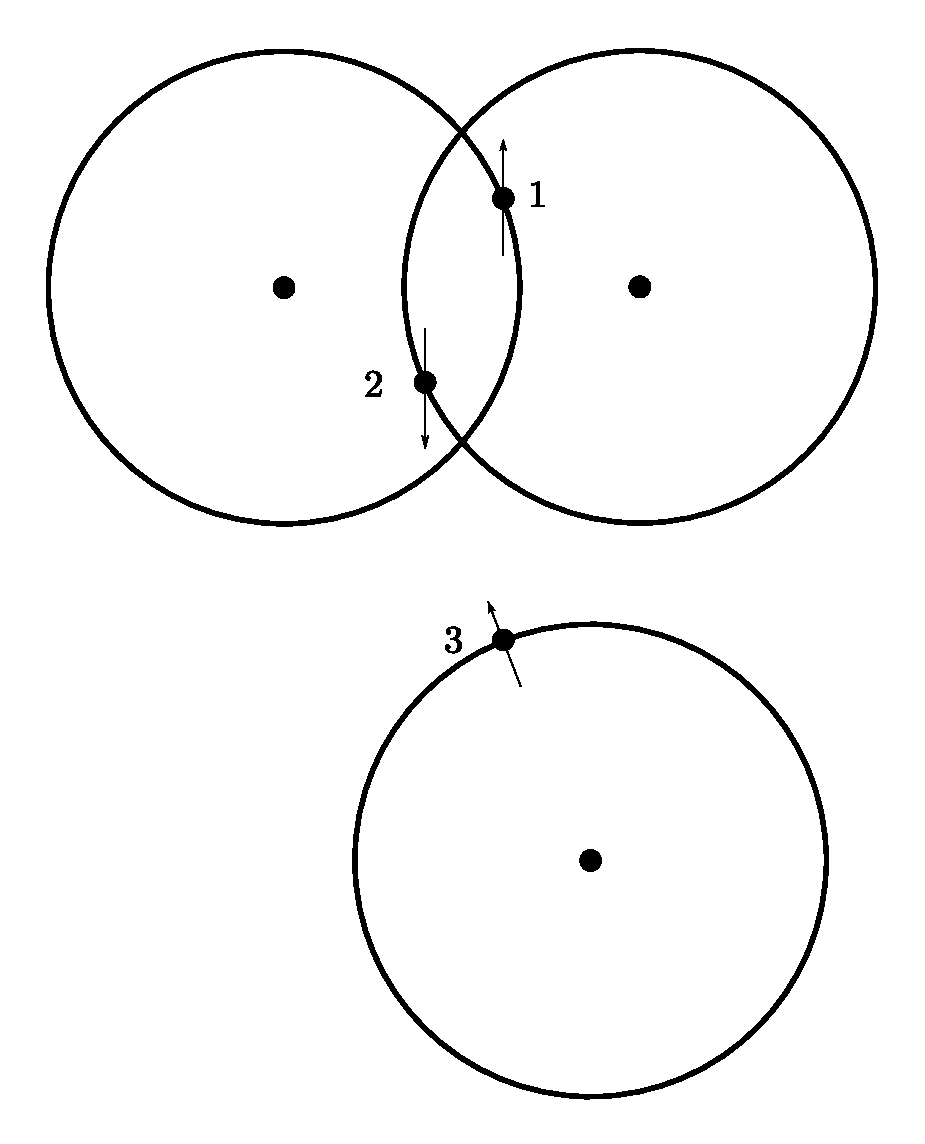
\includegraphics[width=2.5cm,clip]{QM file/figure/10-7}
	\caption{}\label{fig.10-7}
\end{wrapfigure}

共价键最显著的特点是饱和性.设想有第三个氢原子接近一个氢分子.后者的电子对已经处于自旋反对称态,两电子的自旋指向相反,总自旋为0.
外来的第三个电子已经不可能再与它们构成自旋反对称态,所以不能再形成键.从概率观点看问题,两个自旋指向混乱的电子(外来原子的电子与分子中的一个电子,参看图\ref{fig.10-7}),构成自旋对称态(三重态$\chi_{11},\chi_{10},\chi_{1-1}$)的概率是$\frac{3}{4}$,构成自旋反对称态(单态,$\chi_{00}$)的概率是$\frac{1}{4}$,而自旋对称态必为轨道反对称态,原子间的作用$(V^{A})$是排斥的结果是外来原子将受排斥.这就是共价键的饱和性.离子键就没有这种饱和性.

共价键的另一个特点是有方向性.共价键的形成是两个原子的价电子云重叠$(\boldsymbol{r}_{1}\sim\boldsymbol{r}_{2})$的结果,因此形成键的方向总是在价电子云的极大方向.氢原子中电子处于1s态,电子云分布各向同性,没有方向性,第二个原子可以从任何方向接近第一个原子而形成共价键,这种键没有方向性.如果原子的价电子是p态$(l=1)$或d态$(l=2)$电子,其电子云分布就有方向性.以p电子为例,共有3种独立轨道状态,即
\begin{empheq}{equation}\label{eqx5.1}
	\begin{aligned}
		&\varPsi_{npz}=\varPsi_{n10}=zF(r)	\\
	\varPsi_{npx}&=\frac{1}{\sqrt{2}}(\varPsi_{n1-1}-\varPsi_{n11})=xF(r)	\\
	\varPsi_{npy}&=\frac{i}{\sqrt{2}}(\varPsi_{n1-1}+\varPsi_{n11})=yF(r)
	\end{aligned}
\end{empheq}
电子云密度$\varPsi^{2}$的极大方向分别是$x,y,z$轴方向,如另一个原子的价电子(设为s电子)与这样的p电子构成共价键,键的方向必为p电子云的极大方向,如图\ref{fig.10-8}所示.

\begin{figure}[!h]
	\centering
	\small
	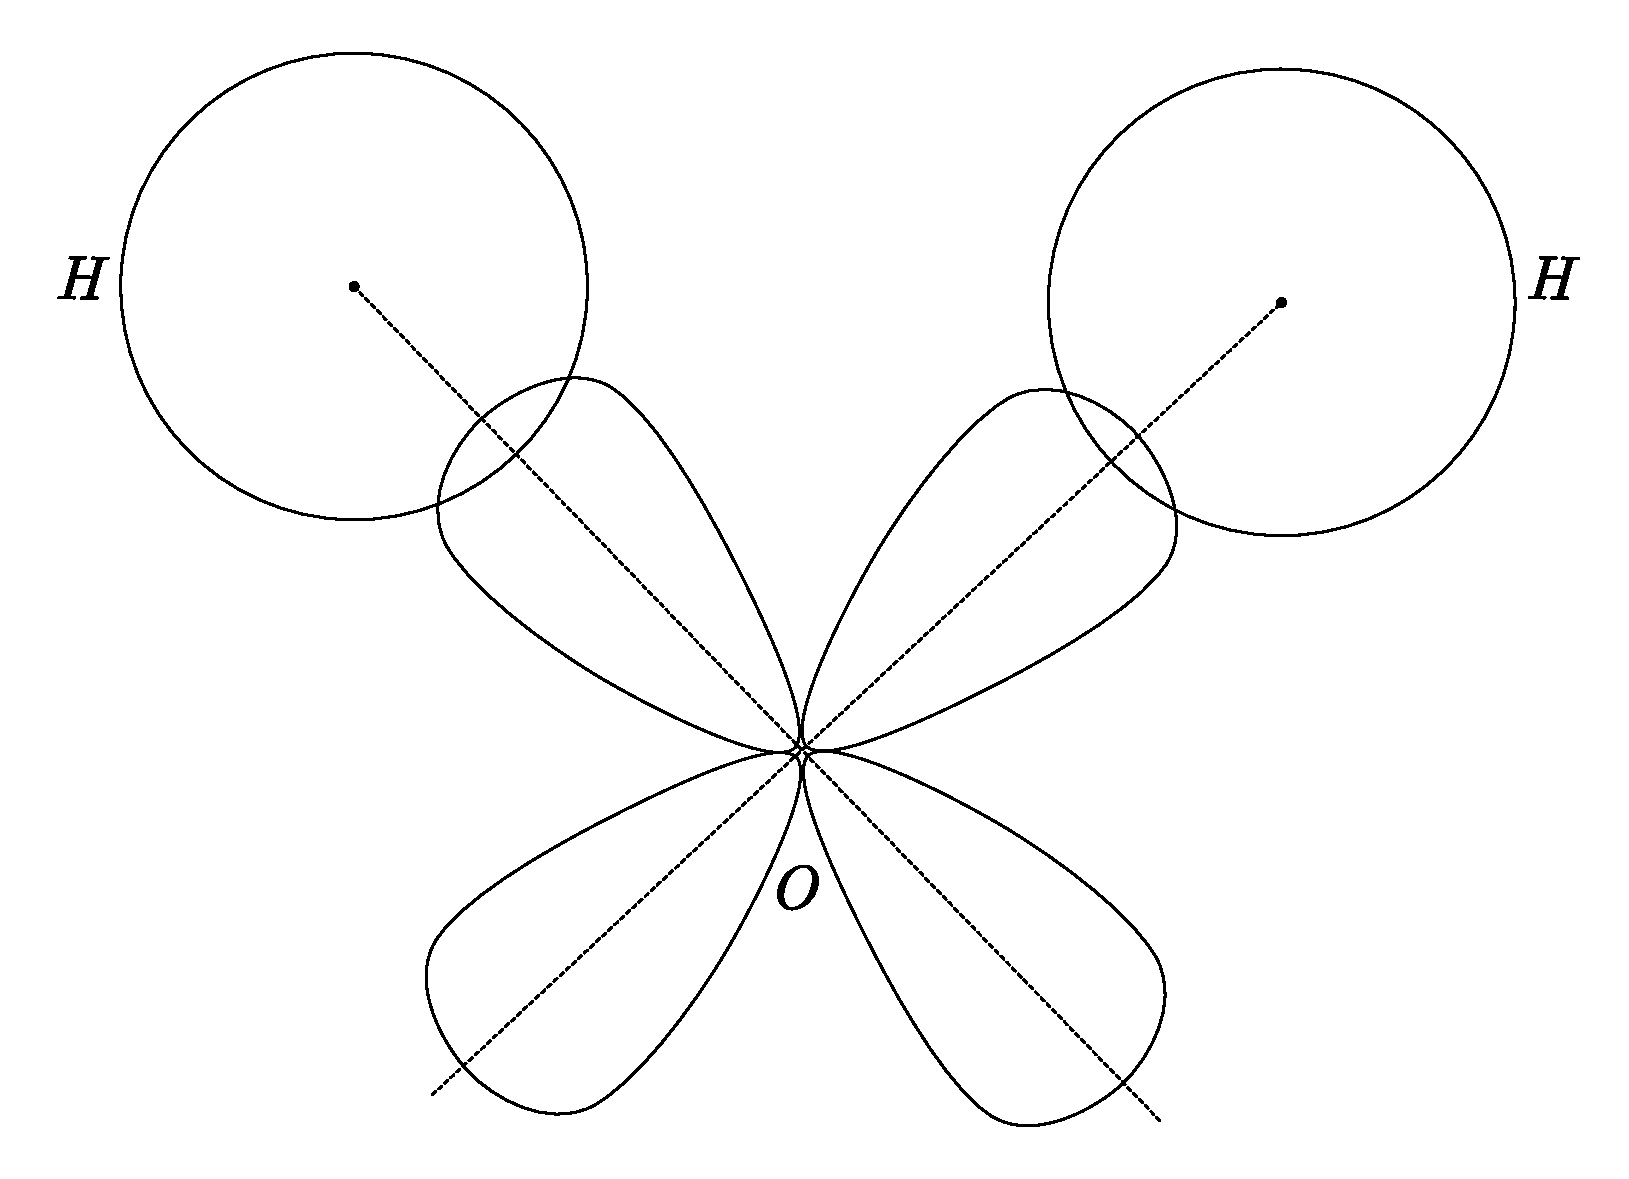
\includegraphics[width=7cm,clip]{QM file/figure/10-8}
	\caption{}\label{fig.10-8}
\end{figure}

以水$\ce{H_{2}O}$分子为例.氧原子中参与$\ce{H-O}$键的两个电子都是p电子,它们电子云的极大方向相互成$90^{\circ}$角.这两个p电子各自和一个氢原子的1s电子结合成共价键,如图\ref{fig.10-8}.由于$\ce{H-O}$键有少量离子键的因素(即$\ce{H^{+}-O^{--}-H^{+}}$),两个氢原子(离子)互相排斥,键角实际上增大成$105^{\circ}$.在19世纪,化学界曾想当然地以为$\ce{H_{2}O}$分子是直线式构造$\ce{H-O-H}$,有了量子化学,键的方向性概念以量子力学为理论依据,才被普遍承认.

在分子中,参与键的电子,由于受到邻近原子的影响,其原子状态严格地说已经与成键前不同.特别是,由于作用势的球对称性(各向同性)遭到破坏,价电子可以不再保持单一的$\boldsymbol{L}^{2}$本征值,其状态可以是s,p,d态的杂化态,这种处于杂化轨道的电子,其电子云分布更容易集中到某个方向,因此更有利于键的形成.量子化学利用杂化轨道理论成功地解释了许多分子构造问题.例如甲烷$(\ce{CH_{4}})$分子,碳$(\ce{C})$原子参与$\ce{C-H}$键的4个电子,本来的原子轨道是$(\ce{2s})^{2}(\ce{2p})^{2}$,由于轨道杂化,它们的单电子轨道态变成如下形式,
\begin{empheq}{equation}\label{eqx5.2}
	\varPsi(\boldsymbol{r})=a\varPsi_{\ce{2s}}+b\varPsi_{\ce{px}}+c\varPsi_{\ce{2py}}+d\varPsi_{\ce{2pz}}
\end{empheq}
当$(a,b,c,d)$取$(1,1,1,1)$,$(1,1,-1,-1)$,$(1,-1,1,-1)$,$(1,-1,-1,1)$时,电子云极大方向刚好是从正四面体中心指向4个顶点的方向,氢原子从这些方向接近,就容易结合成$\ce{C-H}$键.所以$\ce{CH_{4}}$分子中,4个$\ce{H}$原子正好处于正四面体顶点的位置,而$\ce{C}$原子处于对称中心.

半个多世纪以来,由于计算技术的进步和广泛运用量子力学理论及近似方法,量子化学已经发展成一门卓有成效的学科.




% 双原子分子的振动和转动
\starthis\section[双原子分子的振动和转动]{双原子分子的振动和转动} \label{sec:10.06} % 
% \makebox[5em][s]{} % 短题目拉间距

双原子分子的运动包括分子整体平移,转动,振动以及电子在定态能级上的运动和跃迁.如取分子质心坐标系,平移不必考虑电子能级(这里指价电子能级)的量级为10\si{eV}左右,分子振动能级的量级为$0.1\sim 1$\si{eV},转动能级约$10^{-3}\sim 10^{-4}$\si{eV}.例如氧分子$(\ce{O_{2}})$,实验数据为
\eqindent{8}

\begin{empheq}{alignat*=2}
	\text{键长}\num{0.1207}\si{nm}, &\qquad \text{离解能}\num{5.08}\si{eV} 	\\
	\hbar\omega=\num{0.196}\si{eV}, & \qquad \frac{\hbar^{2}}{2I}=\num{1.792}\times10^{-4}\si{eV}	\\
\end{empheq}\eqnormal
研究分子振动和转动时,电子能级一般不会变化,可以将原子当作一个内部结构不变的粒子,两个原子之间的作用以中心作用势$V(r)$表示($r$为两个原子的相对距离),$V-r$关系大体如$\S$\ref{sec:10.04}图\ref{fig.10-5}$\quad V^{5}-R$关系.

在分子质心坐标系中,分子的振动和转动即两原子的相对运动,等效于质量为$\mu$(折合质量)的粒子在中心势场$V(r)$中的运动,(参看$\S$\ref{sec:10.01})这个等效粒子的能量算符为
\begin{empheq}{equation}\label{eqx6.1}
	H=-\frac{\hbar^{2}}{2\mu}\nabla^{2}+V(r)
\end{empheq}
$V(r)$即两个原子间借以结合成分子的作用势,相当于$\S$\ref{sec:10.04}图\ref{fig.10-5}中的$V^{5}$.\eqref{eqx6.1}式中$(-i\hbar)\nabla$即二原子体系的相对动量$(\boldsymbol{p})$算符.相对角动量$\boldsymbol{L}=\boldsymbol{r}\times\boldsymbol{p}=-i\hbar\boldsymbol{r}\times\nabla$也就是分子的轨道角动量$(\boldsymbol{L}_{c}=0)$.$H,\boldsymbol{L}^{2},L_{z}$的共同本征函数可以表示成(参看$\S$\ref{sec:05.01})
\begin{empheq}{equation}\label{eqx6.2}
	\varPsi=R(r)Y_{lm}(\theta,\varphi)=\frac{1}{r}u(r)Y_{lm}(\theta,\varphi)
\end{empheq}
其中球谐函数$Y_{lm}$描写分子转动.$u(r)$满足径向方程
\begin{empheq}{equation}\label{eqx6.3}
	-\frac{\hbar^{2}}{2\mu}\frac{d^{2}}{dr^{2}}u+\left[V(r)+\frac{l(l+1)\hbar^{2}}{2\mu r^{2}}\right]u=Eu
\end{empheq}
$u(r)$描述相对径向运动,即振动.$E$为总能量,即振动,转动能量的总和再加上分子结合能[下面\eqref{eqx6.4}式中$V_{0}$.]

设分子键长为$R$,则$r=R$处$V(r)$为极小.如振动的振幅很小,即$|r-R\ll R$,可将$V(r)$展开成$(r-R)$的幕级数而略去$(r-R)^{3}$以上各项,取
\begin{empheq}{align}\label{eqx6.4}
	V(r)&=V_{0}+\frac{1}{2}V^{\prime\prime}(R)(r-R)^{2}	\nonumber\\
	&=V_{0}+\frac{1}{2}\mu\omega_{0}^{2}(r-R)^{2}
\end{empheq}
$V_{0}$即$V(R)$.将\eqref{eqx6.4}式代入\eqref{eqx6.3}式,得到
\begin{empheq}{align}
	-\frac{\hbar^{2}}{2\mu}\frac{d^{2}}{dr^{2}}u+V_{l}(r)u=(E-V_{0})u	\label{eqx6.5}\\
	V_{l}(r)=\frac{1}{2}\mu\omega_{0}^{2}(r-R)^{2}+\frac{l(l+1)\hbar^{2}}{2\mu r^{2}}	\label{eqx6.6}
\end{empheq}
$(E-V_{0})$为振动与转动能量之和,$V_{l}(r)$是等效势能.当$r=R$,$V_{l}$中第二项(离心势能)即通常所说分子转动能级,记为$E_{l}$
\begin{empheq}{equation}\label{eqx6.7}
	E_{l}=\frac{l(l+1)\hbar^{2}}{2\mu R^{2}}=\frac{l(l+1)\hbar^{2}}{2I}
\end{empheq}\eqshort
$I=\mu R^{2}$为分子转动惯量.设
\begin{empheq}{equation}\label{eqx6.8}
	E_{l}\ll \frac{1}{2}\mu\omega_{0}^{2}R^{2}
\end{empheq}\eqnormal
(上式右端相当于振动的振幅等于键长$R$时的振动能,这样大的能量足以使分子离解.所以上式总是成立的.)在这条件下$V_{l}$将存在极小,其位置可由极值条件$\frac{dV_{l}}{dr}=0$来确定,如下.
\begin{empheq}{align}\label{eqx6.9}
	\frac{d}{dr}V_{l}(r) &=\mu\omega_{0}^{2}(r-R)-\frac{l(l+1)\hbar^{2}}{\mu r^{3}}	\nonumber\\
	&\approx\mu\omega_{0}^{2}(r-R)-\frac{l(l+1)\hbar^{2}}{\mu R^{3}}=0	\nonumber\\
	r&=R+\frac{l(l+1)\hbar^{2}}{\mu^{2}\omega_{0}^{2}R^{3}}\xlongequal{\text{令}}r_{0}
\end{empheq}
如将$R$看成分子的静态(振动、转动完全消失)键长,则$r_{0}$就是动态键长,其中第二项是由于转动而引起的键的伸长.将$V_{l}(r)$在$r_{0}$附近展开成$(r-r_{0})$的幕级数,略去$(r-r_{0})^{3}$以上各项,得到
\begin{empheq}{equation}\label{eqx6.10}
	V_{l}(r)=V_{l}(r_{0})+\frac{1}{2}V_{l}^{\prime\prime}(r_{0})(r-r_{0})^{2}
\end{empheq}
如令
\begin{empheq}{equation}\label{eqx6.11}
	x=r-r_{0},\quad V_{l}^{\prime\prime}=\mu\omega_{0}^{2}
\end{empheq}
即得
\begin{empheq}{equation*}\label{eqx6.10'}
	V_{l}(r)=V_{l}(r_{0})+\frac{1}{2}\mu\omega_{0}^{2}x^{2}
	\tag{$10.6.10^{\prime}$}
\end{empheq}\eqlong
代入径向方程\eqref{eqx6.5}式,成为
\begin{empheq}{equation}\label{eqx6.12}
	-\frac{\hbar^{2}}{2\mu}\frac{d^{2}}{dx^{2}}+\frac{1}{2}\mu\omega^{2}u=[E-V_{0}-V_{l}(r_{0})]u=E^{\prime}u
\end{empheq}\eqllong
上式形式上和一维谐振子的能量本征方程相同,利用谐振子能级公式,即可得出
\begin{empheq}{equation}\label{eqx6.13}
	E-V_{0}-V_{l}(r_{0})=E^{\prime}=\left(\nu+\frac{1}{2}\right)\hbar\omega,\quad \nu=0,1,2,\cdots
\end{empheq}\eqlong
$\nu$为振动量子数.由\eqref{eqx6.6}、\eqref{eqx6.9}式容易求出
\begin{empheq}{align}\label{eqx6.14}
	V_{l}(r_{0}) &=\frac{1}{2}\mu\omega_{0}^{2}\left[\frac{l(l+1)\hbar^{2}}{\mu^{2}\omega_{0}^{2}R^{3}}\right]+\frac{l(l+1)\hbar^{2}}{2\mu r_{0}^{2}}	\nonumber\\
	&\approx E_{l}-\frac{l^{2}(l+1)^{2}\hbar^{4}}{2\mu^{2}\omega_{0}^{2}R^{6}}
\end{empheq}\eqindent{11}
计算中作了近似处理
\begin{empheq}{equation*}
	\frac{1}{r_{0}^{2}}\approx\frac{1}{R^{2}}-\frac{2l(l+1)\hbar^{2}}{\mu^{2}\omega_{0}^{2}R^{6}}
\end{empheq}
由\eqref{eqx6.6}、\eqref{eqx6.9}、\eqref{eqx6.11}式可以求出
\begin{empheq}{align}\label{eqx6.15}
	\omega^{2} &=\omega_{0}^{2}+\frac{3l(l+1)\hbar^{2}}{\mu^{2}r_{0}^{4}} \nonumber\\
	\omega&\approx\omega_{0}+\frac{3l(l+1)\hbar^{2}}{2\mu^{2}\omega_{0}R^{4}}
\end{empheq}\eqnormal
其中第二项是由于转动而引起的振动频率变化.将以上结果代入\eqref{eqx6.13}式,即得分子振-转能级的最后表达式
\begin{empheq}{equation}\label{eqx6.16}
	\begin{aligned}
	E_{\nu l}&=E-V_{0}=V_{l}(r_{0})+\left(\nu+\frac{1}{2}\right)\hbar\omega	\\
	&\approx\left(\nu+\frac{1}{2}\right)\hbar\omega+E_{l}-\frac{l^{2}(l+1)^{2}\hbar^{4}}{2\mu^{2}\omega_{0}^{2}R^{6}}	\\
	E_{l}&=\frac{l(l+1)\hbar^{2}}{2\mu R^{2}},\quad l,\nu=0,1,2,\cdots
	\end{aligned}
\end{empheq}
$E_{l}$即上述转动能级,$\left(\nu+\frac{1}{2}\right)\hbar\omega$常称为振动能级,$E_{\nu l}$中最后一项则是由于键长改变而产生的能级修正,称为振-转修正项.


% 习题
\begin{exercises}

\exercise 两个质量为$m$的全同粒子,在一维弹性力场中运动,$V_{1}=\dfrac{kx_{1}^{2}}{2},V_{2}=\dfrac{kx_{2}^{2}}{2}$,两粒子间的相互作用可以忽略.

(a) 写出体系的总能量算符,分别用$(x_{1},x_{2})$表示和$(X,x)$表示.($X$是质心坐标,$x$是相对坐标)讨论质心运动和相对运动的性质.

(b) 写出单粒子运动的基态与第一激发态波函数.($\varPsi_{0}$与$\varPsi_{1}$,略去归一化常数)如一个粒子处于基态,一个粒子处于第一激发态,写出对称的和反对称的体系轨道波函数,先用$(x_{1},x_{2})$表示,再用$(X,x)$表示,解释其性质.
\pskip
\exercise 两个质量为$m$的非全同粒子,受到外场作用,还有相互作用,作用势为
\eqllong
\begin{empheq}{equation*}
	V_{1}=\frac{\alpha}{2}x_{1}^{2},\quad V_{2}=\frac{\alpha}{2}x_{2}^{2},\quad V_{12}=\frac{\beta}{2}(x_{1}^{2}-x_{2}^{2})\quad (\alpha,\beta>0)
\end{empheq}\eqnormal

求体系的能谱.
\pskip
\exercise 某体系由3个自旋为0的全同粒子组成,限定单粒子状态只能是$\varPsi_{\alpha},\varPsi_{\beta},\varPsi_{\gamma}$,试写出体系的所有可能状态的波函数.

\exercise 两个自旋为0的全同粒子在无限深势阱$(0<x_{i}<a,i=1,2)$中运动,忽略粒子间相互作用.写出这个二粒子体系的基态与第一激发态波函数,并对基态计算$\bar{x},\Delta x,\bar{X},\Delta X$.

[提示:先计算$\bar{x_{1}},\bar{x_{2}},\bar{x_{1}^{2}},\bar{x_{2}^{2}}$.]
\pskip
\exercise 两个质量相同的粒子在无限深势阱$(0<x_{i}<a,i=1,2)$中运动.粒子间相互作用势$V_{12}=aV_{0}\delta(x_{1}-x_{2}),V_{0}\ll\dfrac{\hbar^{2}}{ma^{2}}$,因此可以视之为微扰.求这二粒子体系最低的3个能级.(不考虑粒子是否全同.)
\pskip
\exercise 类氦离子由原子核(电荷$Ze,Z>2$)及两个电子构成.如略去核运动,二电子体系总能量算符可以写成
\begin{empheq}{equation*}
	H=-\frac{\hbar^{2}}{2m_{e}}(\nabla_{1}^{2}+\nabla_{2}^{2})-Z\e^{2}\left(\frac{1}{r_{1}}+\frac{1}{r_{2}}\right)+\frac{\e^{2}}{r_{12}}
\end{empheq}\eqllong

(a) 视$\dfrac{\e^{2}}{r_{12}}$为微扰,求基态能级的粗略近似.

(b) 用变分法求基态能级近似值.
\pskip
\exercise 有-种简化的“一维类氦离子”模型,原子核-电子和电子-电子作用势均用“接触作用”表示.略去核运动后,电子体系总能量算符表示成
\begin{empheq}{equation*}
	H=-\frac{\hbar^{2}}{2m_{e}}\left(\frac{\partial^{2}}{\partial x_{1}^{2}}+\frac{\partial^{2}}{\partial x_{2}^{2}}\right)-Z\e^{2}[\delta(x_{1})+\delta(x_{2})]+\e^{2}\delta(x_{1}-x_{2})
\end{empheq}\eqlong

如距离以$\dfrac{a_{0}}{Z}$为单位,能量以$\dfrac{Z^{2}\e^{2}}{a_{0}}$为单位,$H$可以简化成
\begin{empheq}{equation*}
	H=-\frac{1}{2}\left(\frac{\partial^{2}}{\partial x_{1}^{2}}+\frac{\partial^{2}}{\partial x_{2}^{2}}\right)-\delta(x_{1})-\delta(x_{2})+\frac{1}{Z}\delta(x_{1}-x_{2})
\end{empheq}

(a) 视电子-电子作用势为微扰,求体系束缚态能级(只有一个).

(b) 用变分法求体系能级.

你将发现本题结果与10-6题结果惊人地接近.
\pskip
\exercise 某个三电子体系,单电子轨道态为$\varPsi_{a},\varPsi_{b},\varPsi_{c}$.当体系总自旋量子数$S=\dfrac{3}{2}$时,写出体系的轨道波函数,求相互作用能$\left(\dfrac{\e^{2}}{r_{12}}+\dfrac{\e^{2}}{r_{23}}+\dfrac{\e^{2}}{r_{31}}\text{的平均值}\right)$,将其表示成“库仑能”和“交换能”.
\pskip
\exercise 由两个全同粒子组成的体系,如单粒子自旋量子数为S,$[\boldsymbol{S}^{2}=S(S+1)\hbar^{2}]$体系总自旋态有多少种独立的交换对称态、反对称态?
\pskip
\exercise (a) 如原子中的电子换成某种电荷为$(-e)$,自旋量子数为$\dfrac{3}{2}$的粒子,求前三种惰性气体的原子序数($Z$,核中质子数)

(b) 如原子中的电子换成某种电荷为$(-\dfrac{e}{3})$,自旋量子数为$\dfrac{1}{2}$的费密子,求前三种惰性气体的原子序数.
\pskip
\exercise 两电子体系,定义“自旋交换算符”$P_{12},P_{12}\chi(S_{1z},S_{2z})=\chi(S_{2z},S_{1z})$,证明:$P_{12}=\dfrac{1}{2}(1+\boldsymbol{\sigma}_{1}\cdot\boldsymbol{\sigma}_{2})=\boldsymbol{S}^{2}-1$.($\boldsymbol{S}$为总自旋,取$\hbar=1$)
\pskip
\exercise 设粒子1,2自旋量子数均为$\dfrac{1}{2}$,以$\boldsymbol{S}=\boldsymbol{S}_{1}+\boldsymbol{S}_{2}$表示总自旋算符,取$\hbar=1$.证明以下算符关系:

\begin{empheq}{alignat*=2}
	[\boldsymbol{S}_{1}\cdot\boldsymbol{S}_{2},\boldsymbol{S}_{1}]=i\boldsymbol{S}_{1}\times\boldsymbol{S}_{2}, &\quad [\boldsymbol{S}_{1}\cdot\boldsymbol{S}_{2},\boldsymbol{S}_{2}]=-i\boldsymbol{S}_{1}\times\boldsymbol{S}_{2}	\\
	[\boldsymbol{S}_{1}\cdot\boldsymbol{S}_{2},\boldsymbol{S}]=0, &\quad  \boldsymbol{S}\boldsymbol{S}^{2}=\boldsymbol{S}^{2}\boldsymbol{S}=2\boldsymbol{S}	\\
\end{empheq}\eqnormal

\exercise 两个自旋量子数为$\dfrac{1}{2}$的非全同粒子,位置固定,相互作用能(算符)为$H=\dfrac{\omega}{\hbar}\boldsymbol{S}_{1}\cdot\boldsymbol{S}_{2}$时粒子1自旋$(\boldsymbol{S}_{1})$沿正$z$轴方向极化,粒子2自旋$(\boldsymbol{S}_{2})$极化方向正好相反.对于任意$t>0$时刻,

(a) 求体系总自旋波函数$\chi(t)$,用单粒子自旋态$\alpha(1),\beta(1),\alpha(2),\beta(2)$表示出来,[提示:将初始总自旋态展开成$H$的本征态的叠加.]

(b) 求$\boldsymbol{S}_{1}$极化方向与初始指向相同的概率.

(c) 求$\boldsymbol{S}_{1}$和$\boldsymbol{S}_{2}$极化方向均指向正$z$轴的概率.

(d) 总自旋量子数$S=1,0$的各自概率.
\pskip
\exercise 如原子的最外层是两个单粒子能级为$E_{nl}$的电子,作为二电子体系,讨论其总$L,S,J$的可能取值组合,证明$L+S=$偶数.

[提示:注意波函数的交换对称性,同时参看$\S$\ref{sec:10.02}例题.]
\pskip
\exercise 已知氘核(d)自旋为$\hbar$,宇称为偶;中子(n)自旋为$\dfrac{\hbar}{2}$;$\pi^{-}$介子自旋为0.试根据反应
\begin{empheq}{equation*}
	\pi^{-}\text{(静止)}+\ce{d}\rightarrow \ce{n}+\ce{n}
\end{empheq}

决定$\pi^{-}$介子的内禀宇称.

[提示:反应前后角动量守恒,宇称守恒.反应后为费密子体系.]
\pskip
\exercise 考虑一个多电子原子或分子,总能量包括各个电子及原子核的动能以及粒子间的库仑势能.(忽略自旋和相对论效应)体系的基态能级记为$E_{0}$,基态波函数记为$\varPsi_{0}$,预备用变分法找$E_{0}$,$\varPsi_{0}$的近似.设己找到$\varPsi_{0}$的粗略近似$\phi(\boldsymbol{r}_{1},\boldsymbol{r}_{2},\cdots,\boldsymbol{r}_{N})$,并已求出体系动能平均值$W$,势能平均值$U<0$,再取试探波函数为$\varPsi(\lambda)=\lambda^{\dfrac{3N}{2}}\phi(\lambda\boldsymbol{r}_{1},\cdots,\lambda\boldsymbol{r}_{N})$.证明:

(a) $\lambda$最佳值为$\lambda_{0}=-\dfrac{U}{2W}$,$E_{0}$近似值$E(\lambda_{0})=-\dfrac{U^{2}}{4W}$.

(b) 如$\phi(\boldsymbol{r}_{1},\cdots,\boldsymbol{r}_{N})$刚好就是$\varPsi_{0}$,则$U=-2W,E_{0}=W+U$(即位力定理结论)试将本题结论用于氦原子,利用微扰论结果直接得出变分法结果.

\end{exercises}


% 附录1 δ函数和傅里叶变换
\clearpage
\appendix

%\renewcommand\chaptername{Appendix}
%\renewcommand\thechapter{\arabic{chapter}}


%\renewcommand\chaptername{Appendix}            % hereafter, chapters are called "Appendix"
%\renewcommand\thechapter{\Alph{chapter}}       % chapter number in alph letters
%\renewcommand\thesection{\Alph{chapter}.\Roman{section}} % make sections "A.I"

%\renewcommand{\appendixname}{Appendix~\arabic{section}}

\setcounter{chapter}{0}
\setcounter{figure}{0}
\chapter{δ函数和傅里叶变换}	\label{A01}

% 更改公式标号格式
\counterwithout{equation}{chapter}		% 移除于chapter关联


% 正文

在这里我们不准备叙述$\delta$函数的严格数学理论,而只是将它作为一种方便的数学工具介绍给读者.

{\heiti 1. $\delta$函数的定义及基本性质}

以$f(x)$表示任何具有良好解析性质的函数.规定$\delta$函数的基本性质(也就是定义)为
\eqlong
\begin{empheq}{equation}\label{eqA1.1}
	\boxed{ \int_{a}^{b}f(x)\delta(x-x_{0})dx=f(x_{0}),\quad a<x_{0}<b
	}
\end{empheq}\eqnormal
显然,这定义等价于下列定义:
\begin{empheq}{align}\label{eqA1.2}
	&\int_{-\infty}^{\infty}f(x)\delta(x-x_{0})dx	\nonumber\\
	=&\int_{x_{0}-\varepsilon}^{x_{0}+\varepsilon}f(x)\delta(x-x_{0})dx=f(x_{0})
\end{empheq}
其中$\varepsilon$为任意小正数.通常,还可改用下列等价定义:
\begin{empheq}{equation}\label{eqA1.3}
	\begin{dcases}
		\delta(x-x_{0})=0,x\neq x_{0}	\\
		\int_{-\infty}^{\infty}\delta(x-x_{0})dx=1
	\end{dcases}
\end{empheq}\eqshort
容易证明,$\delta(x)$是偶函数,$\delta(x)=\delta(-x)$,并有性质
\begin{empheq}{equation}\label{eqA1.4}
	\delta(\lambda x)=\frac{1}{|\lambda|}\delta(x)
\end{empheq}
这公式在积分换元时很有用.

在\eqref{eqA1.1}式中取$f(x)=x-x_{0}$,则$f(x_{0})=0$,这结果适用于任何积分区间$(a,b)$,所以等价于
\begin{empheq}{equation}\label{eqA1.5}
	(x-x_{0})\delta(x-x_{0})=0
\end{empheq}\eqllong


{\heiti 2. $\delta$函数的具体表示}

某些含参数的函数,当参数趋于某种极限时,就成为$\delta$函数.最常用的有下列几种
\begin{empheq}{equation}\label{eqA1.6}
(\ce{i})\qquad\qquad\qquad \delta(x)=\lim\limits_{\alpha\rightarrow0}\frac{1}{\sqrt{\pi}\alpha}e^{-x^{2}/\alpha}
\end{empheq}
这个函数符合定义\eqref{eqA1.3}式,其图形如附录图1所示,曲线下面的面积为1,有效宽度大致为$2\alpha$.
\begin{empheq}{equation}\label{eqA1.7}
(\ce{ii})\qquad\qquad\qquad \boxed{\delta(x)=\lim_{\alpha\rightarrow\infty}\frac{\sin\alpha x}{\pi x} }
\end{empheq}\eqnormal
其图形如附录图2所示,为振荡衰减型,有效宽度大致为$\frac{2\pi}{\alpha}$.在$|x|>\frac{\pi}{\alpha}$区域,由于迅速振荡,对积分无贡献.而全空间积分等于1:
\begin{empheq}{equation*}
	\int_{-\infty}^{\infty}\frac{\sin\alpha x}{\pi x}dx=\frac{1}{\pi}\int_{-\infty}^{\infty}\frac{\sin t}{t}dt=1.
\end{empheq}\eqllong
\begin{figure}[!h]
	\centering
	\small
	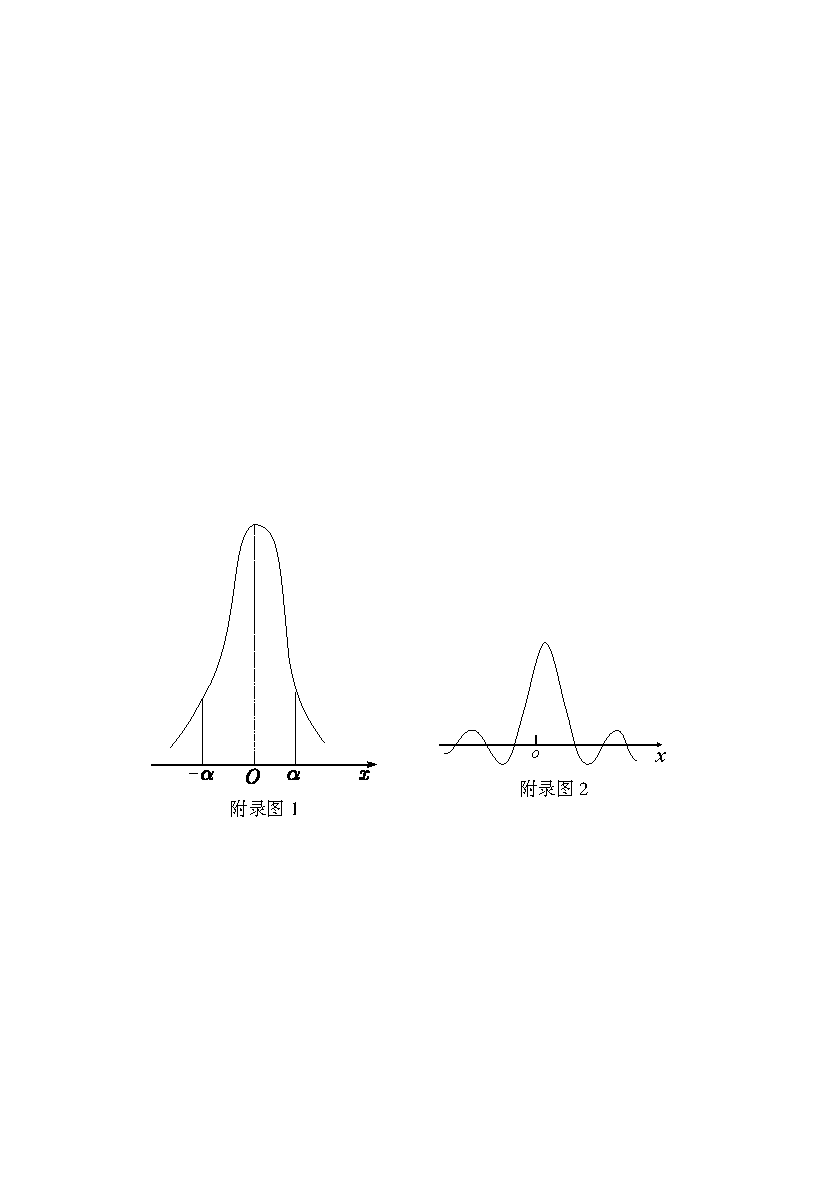
\includegraphics[width=8cm,clip]{QM file/figure/A-1,2}
	\caption*{}\label{fig.A-1,2}
\end{figure}
\begin{empheq}{equation}\label{eqA1.8}
(\ce{iii})\qquad\qquad\qquad \boxed{\delta(x)=\frac{1}{2\pi}\int_{-\infty}^{\infty}e^{ikx}dk }
\end{empheq}\eqnormal
由于$e^{ikx}=\cos kx+i\sin kx$,如将\eqref{eqA1.8}式中积分上下限改写为$\pm\alpha(\alpha\rightarrow\infty)$,立即可以发现\eqref{eqA1.8}式与\eqref{eqA1.7}式是等价的.

{\heiti 3. 傅里叶变换}

将任何具有良好解析性质的函数$f(x)$表示成傅里叶积分的形式
\begin{empheq}{equation}\label{eqA1.9}
	f(x)=\frac{1}{\sqrt{2}}\int_{-\infty}^{\infty}g(k)e^{ikx}dk
\end{empheq}\eqlllong
$g(k)$称为$f(x)$的傅里叶变换式.利用$\delta$函数很容易导出$g(k)$的公式,如下.利用\eqref{eqA1.8}式,将$f(x)$表示成
\begin{empheq}{align*}
	f(x)&=\int_{-\infty}^{\infty}f(x^{\prime})\delta(x-x^{\prime})dx^{\prime}
	&=\frac{1}{2\pi}\iint_{-\infty}^{\infty}f(x^{\prime})e^{ik(x-x^{\prime})}dkdx^{\prime}
\end{empheq}\eqnormal
与\eqref{eqA1.9}式比较,即得
\begin{empheq}{align}\label{eqA1.10}
	g(k)&=\frac{1}{\sqrt{2}}\int_{-\infty}^{\infty}f(x^{\prime})e^{-ikx^{\prime}}dx^{\prime}	\nonumber\\
	&=\frac{1}{\sqrt{2}}\int_{-\infty}^{\infty}f(x)e^{-ikx}dx
\end{empheq}
此即傅里叶变换式.注意\eqref{eqA1.9}、\eqref{eqA1.10}式结构的对称性.

{\heiti 4. 三维情形}

三维$\delta$函数定义为
\begin{empheq}{equation}\label{eqA1.11}
	\delta(\boldsymbol{r}-\boldsymbol{r}_{0})=\delta(x-x_{0})\delta(y-y_{0})\delta(z-z_{0})
\end{empheq}
其中
\begin{empheq}{equation*}
	\boldsymbol{r}=(x,y,z),\quad \boldsymbol{r}_{0}=(x_{0},y_{0},z_{0})
\end{empheq}
基本积分性质为
\begin{empheq}{equation}\label{eqA1.12}
	\boxed{ \iiint_{-\infty}^{\infty}f(\boldsymbol{r})\delta(\boldsymbol{r}-\boldsymbol{r}_{0})d^{3}\boldsymbol{r}=f(\boldsymbol{r}_{0})
	}
\end{empheq}
与\eqref{eqA1.4}式相应,有关系
\begin{empheq}{equation}\label{eqA1.13}
	\delta(\lambda\boldsymbol{r}-\lambda\boldsymbol{r}_{0})=\frac{1}{|\lambda^{3}|}\delta(\boldsymbol{r}-\boldsymbol{r}_{0})
\end{empheq}
\eqref{eqA1.8}式推广成
\begin{empheq}{equation}\label{eqA1.14}
	\delta(\boldsymbol{r})=\frac{1}{(2\pi)^{3}}\iiint_{-\infty}^{\infty}e^{i\boldsymbol{k}\cdot\boldsymbol{r}}d^{3}\boldsymbol{k}
\end{empheq}
利用此式容易导出三维傅里叶变换公式
\begin{empheq}{equation}\label{eqA1.15}
	\boxed{\begin{aligned}
		f(\boldsymbol{r})=\left(\frac{1}{2\pi}\right)^{\frac{3}{2}}\iiint_{-\infty}^{\infty}g(\boldsymbol{k})e^{i\boldsymbol{k}\cdot\boldsymbol{r}}d^{3}\boldsymbol{k}	\\
		g(\boldsymbol{k})=\left(\frac{1}{2\pi}\right)^{\frac{3}{2}}\iiint_{-\infty}^{\infty}f(\boldsymbol{r})e^{i\boldsymbol{k}\cdot\boldsymbol{r}}d^{3}\boldsymbol{r}
	\end{aligned}}
\end{empheq}

采用球坐标$(r,\theta,\varphi)$时,当$r\rightarrow0$,角$\theta,\varphi$失去意义,这时常用径向$\delta$函数$\delta(r)$代替$\delta(\boldsymbol{r})$.考虑到$r$的变化范围是$0\leqslant r<\infty$,$\delta$函数是偶函数,以及$d^{3}\boldsymbol{r}\Rightarrow r^{2}drd\Omega$,
\begin{empheq}{align*}
	 &\iiint_{-\infty}^{\infty}\delta(\boldsymbol{r})d^{3}\boldsymbol{r}=1=2\int_{0}^{\infty}\delta(r)dr	\\
	=&\frac{1}{2\pi}\int d\Omega\int_{0}^{\infty}\frac{\delta(r)}{r^{2}}r^{2}dr	\\
	=&\frac{1}{2\pi}\iiint_{-\infty}^{\infty}\frac{\delta(r)}{r^{2}}d^{3}\boldsymbol{r}
\end{empheq}\eqshort
因此
\begin{empheq}{equation}\label{eqA1.16}
	\delta(\boldsymbol{r})=\frac{1}{2\pi r^{2}}\delta(r)
\end{empheq}\eqnormal
注意
\begin{empheq}{equation}\label{eqA1.17}
	\int_{-\infty}^{\infty}f(r)\delta(r)dr=\frac{1}{2}f(0)
\end{empheq}



% 附录2 厄密多项式
\clearpage
\chapter{厄密多项式}	\label{A02}

令$\xi,\eta$为独立的复变数,考虑下列在整个复平面解析的二元函数
\eqshort
\begin{empheq}{equation}\label{eqA2.1}
	W(\xi,\eta)=e^{2\xi\eta-\eta^{2}}
\end{empheq}
将它展开成$\eta$的幕级数,表示成
\begin{empheq}{equation}\label{eqA2.2}
	W(\xi,\eta)=\sum_{n=0}^{\infty}H_{n}(\xi)\frac{\eta^{n}}{n!}
\end{empheq}
则 
\begin{empheq}{equation*}
	H_{n}(\xi)=\frac{\partial^{n}W}{\partial\eta^{n}}\bigg|_{\eta=0}
\end{empheq}\eqlong
由于
\begin{empheq}{align*}
	W&=e^{2\xi\eta-\eta^{2}}=e^{\eta^{2}-t^{2}},\quad t=\xi-\eta	\\
	\frac{\partial^{n}W}{\partial\eta^{n}}=&(-1)^{n}\frac{\partial^{n}W}{\partial t^{n}}=(-1)^{n}e^{\xi^{2}}\left(\frac{d}{dt}\right)^{n}e^{-t^{2}}	\\
	&\left(\frac{d}{dt}\right)^{n}e^{-t^{2}}|_{\eta=0}=\left(\frac{d}{d\xi}\right)^{n}e^{-\xi^{2}}
\end{empheq}\eqnormal
所以
\begin{empheq}{equation}\label{eqA2.3}
	H_{n}(\xi)=(-1)^{n}e^{\xi^{2}}\left(\frac{d}{d\xi}\right)^{n}e^{-\xi^{2}}
\end{empheq}
显然$H_{n}(\xi)$是$n$次多项式,称为厄密(Hermite)多项式.上式就是它的微分表达式.$W(\xi,\eta)$称为$H_{n}(\xi)$的生成函数或母函数.

\eqref{eqA2.2}式对$\xi$求导,得到
\begin{empheq}{align*}
	\sum_{n}H_{n}^{\prime}(\xi)\frac{\eta^{n}}{n!}&=2\eta W(\xi,\eta)	\\
	&=\sum_{n}2H_{n}(\xi)\frac{\eta^{n+1}}{n!}
\end{empheq}\eqshort
比较上式两端$\eta^{n}$系数,即得
\begin{empheq}{equation}\label{eqA2.4}
	H_{n}^{\prime}(\xi)=2nH_{n-1}(\xi)
\end{empheq}\eqnormal
\eqref{eqA2.2}式对$\eta$求导,经过类似的步骤,得到
\begin{empheq}{equation}\label{eqA2.5}
	2\xi H_{n}(\xi)=H_{n+1}(\xi)+2nH_{n-1}(\xi)
\end{empheq}
以上二式是厄密多项式的基本递推关系.由\eqref{eqA2.4}、\eqref{eqA2.5}式消去$H_{n-1}$,再对$\xi$求导,再利用\eqref{eqA2.4}式消去$H_{n+1}^{\prime}$,就得$H_{n}$满足的微分方程
\begin{empheq}{equation}\label{eqA2.6}
	H_{n}^{\prime\prime}(\xi)-2\xi H_{n}^{\prime}(\xi)+2nH_{n}(\xi)=0
\end{empheq}
称为厄密方程.\eqref{eqA2.3}式是这个方程的唯一多项式解.

将\eqref{eqA2.2}式中$\eta$换成另一个变数$s$,
\begin{empheq}{equation*}
	e^{2\xi s-s^{2}}=\sum_{m=0}^{\infty}H_{m}(\xi)\frac{s^{m}}{m!}
\end{empheq}
与\eqref{eqA2.2}式相乘,得到
\begin{empheq}{align*}
	&\sum_{n}\sum_{m}H_{n}(\xi)H_{m}(\xi)\frac{\eta^{n}s^{m}}{n!m!}	\\
	=&\exp(2\xi\eta+2\xi s-\eta^{2}-s^{2})	\\
	=&\exp[\eta^{2}+2\eta s-(\xi-\eta-s)^{2}]
\end{empheq}
以$e^{-\xi^{2}}$乘上式两端,并积分$\int_{-\infty}^{\infty}\cdots d\xi$,得到
\begin{empheq}{align*}
	&\sum_{n}\sum_{m}\frac{\eta^{n}s^{m}}{n!m!}\int_{-\infty}^{\infty}e^{-\xi^{2}}H_{n}(\xi)H_{m}(\xi)d\xi	\\
=& e^{2\eta s}\int_{-\infty}^{\infty}e^{-(\xi-\eta-s)^{2}}d\xi	\\
=& e^{2\eta s}\int_{-\infty}^{\infty}e^{-x^{2}}dx=\sqrt{\pi}e^{2\eta s}	\\
=& \sqrt{\pi}\sum_{n=0}^{\infty}2^{n}\frac{(\eta s)^{n}}{n!}
\end{empheq}
比较上式两端,即得厄密多项式的正交归一化公式
\begin{empheq}{equation}\label{eqA2.7}
	\int_{-\infty}^{\infty}e^{-\xi^{2}}H_{n}(\xi)H_{m}(\xi)d\xi=2^{n}n!\sqrt{\pi}\delta_{nm}
\end{empheq}
其中$e^{-\xi^{2}}$为权函数.换言之,下列函数系$\{\phi_{n}(\xi)\}$是$-\infty<\xi<\infty$区域的正交归一化完备函数系:
\begin{empheq}{equation}\label{eqA2.8}
	\phi_{n}(\xi)=(2^{n}n!\sqrt{\pi})^{-\frac{1}{2}}e^{-\xi^{2}/2}H_{n}(\xi)
\end{empheq}
由\eqref{eqA2.3}式可知,$H_{n}(\xi)$及$\phi_{n}(\xi)$的宇称为$(-1)^{n}$,即
\begin{empheq}{align}
	H_{n}(-\xi)=(-1)^{n}H_{n}(\xi)		\label{eqA2.9}\\
	\phi_{n}(-\xi)=(-1)^{n}\phi_{n}(\xi)		\label{eqA2.10}
\end{empheq}\eqlong
前几种厄密多项式是
\begin{empheq}{equation}\label{eqA2.11}
	\begin{aligned}
		H_{0}&(\xi)=1,\quad H_{1}(\xi)=2\xi	\\
		H_{2}(\xi)=&4\xi^{2}-2,\quad H_{3}(\xi)=8\xi^{3}-12\xi	\\
		H_{4}&(\xi)=16\xi^{4}-48\xi^{2}+12
	\end{aligned}
\end{empheq}\eqnormal
注意,$H_{n}(\xi)$中最高次项是$(2\xi)^{n}$,这一点可从\eqref{eqA2.3}式直接看出.

$H_{n}(\xi)$还有另一种微分表达式,即
\begin{empheq}{equation}\label{eqA2.12}
	H_{n}(\xi)=e^{\eta^{2}/2}\left(\xi-\frac{d}{d\xi}\right)^{n}e^{-\xi^{2}/2}
\end{empheq}
用数学归纳法容易证明\eqref{eqA2.12}式与\eqref{eqA2.3}式是等价的,读者可自行证明之.

% 附录3 轨道角动量算符
\clearpage
\chapter{轨道角动量算符}	\label{A03}

在直角坐标系中,以$\boldsymbol{e}_{1},\boldsymbol{e}_{2},\boldsymbol{e}_{3}$表示$x,y,z$轴方向单位矢量.粒子的位置矢量和梯度算符可以表示成
\begin{empheq}{align}
	&\boldsymbol{r}=x\boldsymbol{e}_{1}+y\boldsymbol{e}_{2}+z\boldsymbol{e}_{3}		\label{eqA3.1}\\
	\nabla&=\boldsymbol{e}_{1}\frac{\partial}{\partial x}+\boldsymbol{e}_{2}\frac{\partial}{\partial y}+\boldsymbol{e}_{3}\frac{\partial}{\partial z}		\label{eqA3.2}
\end{empheq}\eqlong
\begin{wrapfigure}[15]{r}{0.3\textwidth}
	\centering
	\small
	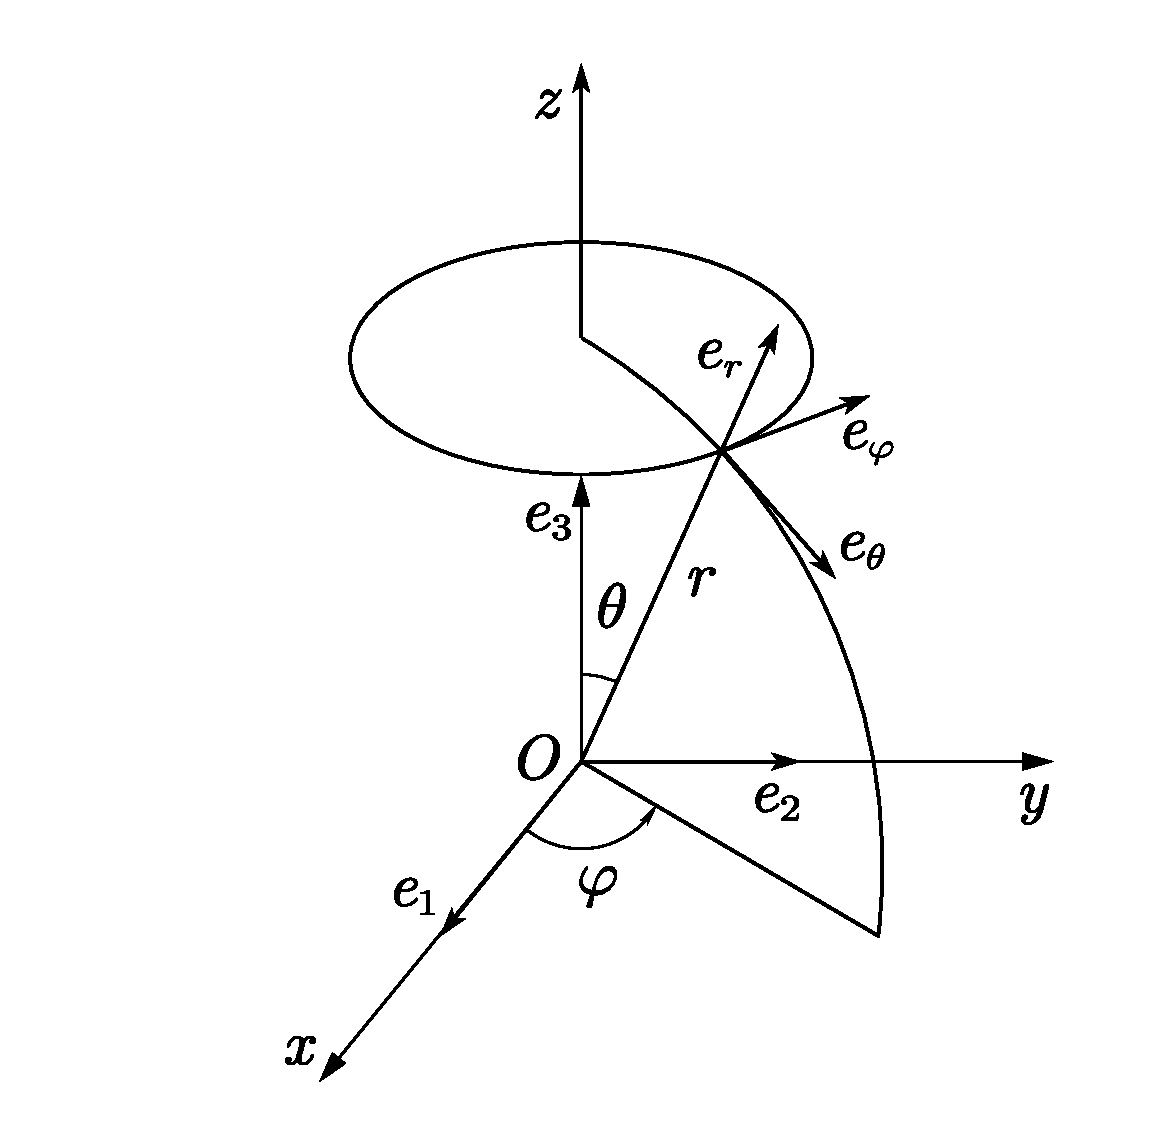
\includegraphics[width=3.5cm,clip]{QM file/figure/A-3}
	\caption*{附录图3}\label{fig.A-3}
\end{wrapfigure}

\noindent 轨道角动量算符为
\begin{empheq}{equation}\label{eqA3.3}
	\boldsymbol{L}=\boldsymbol{r}\times\boldsymbol{p}=-i\hbar\boldsymbol{r}\times\nabla
\end{empheq}\eqindent{1}

在球坐标系中,以$\boldsymbol{e}_{r},\boldsymbol{e}_{\theta},\boldsymbol{e}_{\varphi}$分别表示沿径向,经线切线方向,纬线切线方向单位矢量(附录图3),三者有关系
\begin{equation}\label{eqA3.4}
	\boldsymbol{e}_{r}\times\boldsymbol{e}_{\theta}=\boldsymbol{e}_{\varphi},\quad \boldsymbol{e}_{\theta}\times\boldsymbol{e}_{\varphi}=\boldsymbol{e}_{r},\quad \boldsymbol{e}_{\varphi}\times\boldsymbol{e}_{r}=\boldsymbol{e}_{\theta}
\end{equation}\eqlllong
梯度$\nabla$的球坐标表示为
\begin{equation}\label{eqA3.5}
	\nabla=\boldsymbol{e}_{r}\frac{\partial}{\partial r}+\boldsymbol{e}_{\theta}\frac{1}{r}\frac{\partial}{\partial\theta}+\boldsymbol{e}_{\varphi}\frac{1}{r\sin\theta}\frac{\partial}{\partial\varphi}
\end{equation}\eqnormal
因此,轨道角动量算符可以表示成
\begin{empheq}{align}\label{eqA3.6}
	\boldsymbol{L}&=-i\hbar r\boldsymbol{e}_{r}\times\nabla	\nonumber\\
	&=-i\hbar\left(\boldsymbol{e}_{\varphi}\frac{\partial}{\partial\theta}-\boldsymbol{e}_{\theta}\frac{1}{\sin\theta}\frac{\partial}{\partial\varphi}\right)
\end{empheq}
分别取上式与$\boldsymbol{e}_{1},\boldsymbol{e}_{2},\boldsymbol{e}_{3}$的内积,并注意到
\begin{empheq}{align}\label{eqA3.7}
	\boldsymbol{e}_{1}\cdot\boldsymbol{e}_{\theta}=&\cos\theta\cos\varphi,\quad \boldsymbol{e}_{1}\cdot\boldsymbol{e}_{\varphi}=-\sin\varphi \nonumber\\
	\boldsymbol{e}_{2}\cdot\boldsymbol{e}_{\theta}=&\cos\theta\sin\varphi,\quad \boldsymbol{e}_{2}\cdot\boldsymbol{e}_{\varphi}=\cos\varphi	\nonumber\\
	(&\boldsymbol{e}_{1}\pm i\boldsymbol{e}_{2})\cdot\boldsymbol{e}_{\theta}=\cos\theta\boldsymbol{e}^{\pm i\varphi}	\nonumber\\
	&(\boldsymbol{e}_{1}\pm i\boldsymbol{e}_{2})\cdot\boldsymbol{e}_{\varphi}=\pm i\boldsymbol{e}^{\pm i\varphi}	\nonumber\\		
	\boldsymbol{e}_{3}\cdot\boldsymbol{e}_{\theta}=&-\sin\theta,\quad \boldsymbol{e}_{3}\cdot\boldsymbol{e}_{\varphi}=0
\end{empheq}\eqindent{8}
即得
\begin{empheq}{align}
	L_{x}&=i\hbar\left(\sin\varphi\frac{\partial}{\partial\theta}+\cot\theta\cos\varphi\frac{\partial}{\partial\varphi}\right)		\nonumber\\
	L_{y}&=i\hbar\left(-\cos\varphi\frac{\partial}{\partial\theta}+\cot\theta\sin\varphi\frac{\partial}{\partial\varphi}\right)	\label{eqA3.8}\\
	L_{x}&\pm iL_{y}=\hbar e^{\pm i\varphi}\left(\pm\frac{\partial}{\partial\theta}+i\cot\theta\frac{\partial}{\partial\varphi}\right)		\label{eqA3.9}\\
	L_{z}&=-i\hbar\frac{\partial}{\partial\varphi}		\label{eqA3.10}
\end{empheq}
另外,$\boldsymbol{L}^{2}$可以表示成
\begin{empheq}{align}\label{eqA3.11}
	\boldsymbol{L}^{2}&=L_{x}^{2}+L_{y}^{2}+L_{z}^{2}	\nonumber\\
	&(L_{x}-iL_{y})(L_{z}+iL_{y})+\hbar L_{z}+L_{z}^{2}
\end{empheq}
(利用$L_{x}L_{y}-L_{y}L_{x}=i\hbar L_{z}$)将\eqref{eqA3.9}、\eqref{eqA3.10}式代入上式,经过化简,即得
\begin{empheq}{align}\label{eqA3.12}
	\boldsymbol{L}^{2}&=-\hbar^{2}\left(\frac{\partial^{2}}{\partial\theta^{2}}+\cot\theta\frac{\partial}{\partial\theta}+\frac{1}{\sin^{2}\theta}\frac{\partial^{2}}{\partial\varphi^{2}}\right)	\\
	&=-\hbar^{2}\left(\frac{1}{\sin\theta}\frac{\partial}{\partial\theta}\sin\theta\frac{\partial}{\partial\theta}+\frac{1}{\sin^{2}\theta}\frac{\partial^{2}}{\partial\varphi^{2}}\right)
\end{empheq}\eqlong
采用球坐标时,常令$\cos\theta=\xi$,而以$(r,\xi,\varphi)$作为坐标变量,这时\eqref{eqA3.9}式及\eqref{eqA3.12}式变成
\begin{empheq}{align}
	L_{x}\pm iL_{y}=\hbar e^{\pm i\varphi}\left[\mp(1-\xi^{2})^{\frac{1}{2}}\frac{\partial}{\partial\xi}+i\xi(1-\xi^{2})^{-\frac{1}{2}}\frac{\partial}{\partial\varphi}\right]		\label{eqA3.13}\\
	\boldsymbol{L}^{2}=-\hbar^{2}\left[(1-\xi^{2})\frac{\partial^{2}}{\partial\xi^{2}}-2\xi\frac{\partial}{\partial\xi}+(1-\xi^{2})^{-1}\frac{\partial^{2}}{\partial\varphi^{2}}\right]		\label{eqA3.14}
\end{empheq}\eqnormal

% 附录4 球谐函数
\clearpage
\chapter{球谐函数}\label{A04}

{\heiti 1. 勒让德(Legendre)多项式$P_{l}(\xi)$}

令$\xi,\eta$为独立的实变数.将二元函数$(1-2\xi\eta+\eta^{2})$展开成$\eta$的幕级数,表示成
\begin{empheq}{equation}\label{eqA4.1}
	(1-2\xi\eta+\eta^{2})^{-\frac{1}{2}}=\sum_{l=0}^{\infty}P_{l}(\xi)\eta^{l}
\end{empheq}
展开式中任何一项$\xi$的幕次显然不会超过$\eta$的幕次,因此$P_{l}(\xi)$是$\xi$的$l$次多项式,称为勒让德多项式,上式左端称为$P_{l}(\xi)$的生成函数或母函数.当$|\xi|\leqslant1,|\eta|<1$,展开式\eqref{eqA4.1}显然是收敛的.当$\xi=\pm1$,\eqref{eqA4.1}式成为

\begin{empheq}{equation*}
	\sum_{l}P_{l}(\pm1)\eta^{l}=(1\mp\eta)^{-1}=\sum_{l}(\pm\eta)^{l}
\end{empheq}
因此可知
\begin{empheq}{equation}\label{eqA4.2}
	P_{l}=1,\qquad P_{l}(-1)=(-1)^{l}
\end{empheq}\eqllong
当$\xi=0$,\eqref{eqA4.1}式成为

\begin{empheq}{equation*}
	\sum_{l}P_{l}(0)\eta^{l}=(1+\eta^{2})^{-\frac{1}{2}}=1-\frac{1}{2}\eta^{2}+\frac{3}{8}\eta^{4}-\cdots+\cdots
\end{empheq}\eqnormal
比较两端$\eta^{\prime}$系数,可得
\begin{empheq}{equation}\label{eqA4.3}
	P_{2n}(0)=(-1)^{n}\frac{(2n-1)!!}{(2n)!!},\quad P_{2n+1}(0)=0
\end{empheq}
$P_{l}$的递推关系很多,扼要介绍如下.\eqref{eqA4.1}式对$\eta$求导,可得
\begin{empheq}{equation}\label{eqA4.4}
	(l+1)P_{l+1}+lP_{l-1}=(2l+1)\xi P_{l}
\end{empheq}\eqindent{10}
\eqref{eqA4.1}式对$\xi$求导,则得
\begin{empheq}{equation}\label{eqA4.5}
	P_{l+1}^{\prime}-2\xi P_{l}^{\prime}+P_{l-1}^{\prime}=P_{l}
\end{empheq}
\eqref{eqA4.4}式求导,再与\eqref{eqA4.5}式合并化简,得到
\begin{empheq}{align}
	P_{l+1}^{\prime}&-\xi P_{l}^{\prime}=(l+1)P_{l}		\label{eqA4.6}\\
	\xi &P_{l}^{\prime}-P_{l-1}^{\prime}=lP_{l}		\label{eqA4.7}
\end{empheq}\eqnormal
\eqref{eqA4.6}、\eqref{eqA4.7}式相加,可得到较为对称的公式
\begin{empheq}{equation}\label{eqA4.8}
	P_{l+1}^{\prime}-P_{l-1}^{\prime}=(2l+1)P_{l}
\end{empheq}
\eqref{eqA4.6}式中$l$换成$(l-1)$,再与\eqref{eqA4.7}式合并消去$P_{l-1}^{\prime}$,得到
\begin{empheq}{equation}\label{eqA4.9}
	(1-\xi^{2})P_{l}^{\prime}=lP_{l-1}-l\xi P_{l}
\end{empheq}\eqlong
\eqref{eqA4.9}式与\eqref{eqA4.4}式合并,可得
\begin{empheq}{align}
	&(1-\xi^{2})P_{l}^{\prime}=(l+1)(\xi P_{l}-P_{l+1})		\label{eqA4.10}\\
	(2l+&1)(1-\xi^{2})P_{l}^{\prime}=l(l+1)(P_{l-1}-P_{l+1})	\label{eqA4.11}
\end{empheq}
\eqref{eqA4.9}式求导,再与\eqref{eqA4.7}式合并消去$P_{l-1}^{\prime}$,得到$P_{l}$满足的微分方程
\begin{empheq}{equation}\label{eqA4.12}
	\boxed{ (1-\xi^{2})P_{l}^{n}(\xi)-2\xi P_{l}^{\prime}(\xi)+l(l+1)P_{l}(\xi)=0 }
\end{empheq}\eqnormal
在以上各式中,凡指标为负值时,该项应该删去.[例如\eqref{eqA4.8}式,当$l=0$,成为$P_{1}^{\prime}=P_{0}$]

当$l$较小时,$P_{l}(\xi)$的表达式可以利用\eqref{eqA4.4}式定出,例如
\begin{empheq}{equation*}
	P_{0}=1,\quad P_{1}=\xi,\quad P_{2}=\frac{1}{2}(3\xi^{2}-1)
\end{empheq}
等等.普遍地,$P_{l}$可以表示成
\begin{empheq}{equation}\label{eqA4.13}
	\boxed{ P_{l}(\xi)=\frac{1}{2^{l}l!}\left(\frac{d}{d\xi}\right)^{l}(\xi^{2}-1)^{l} }
\end{empheq}\eqindent{10}
称为罗巨格(Rodrigues)公式.证明如下令$u(\xi)=(\xi^{2}-1)^{l}$,它显然满足方程
\begin{empheq}{equation*}
	(1-\xi^{2})u^{\prime}+2l\xi u=0
\end{empheq}\eqnormal
上式求导$(l+1)$次,利用牛顿-莱布尼茨公式
\begin{empheq}{equation*}
	(uv)^{(n)}=u^{(n)}v+c_{n}^{1}u^{(n-1)}v^{\prime}+c_{n}^{2}u^{(n-2)}v^{\prime\prime}+\cdots
\end{empheq}
($u^{(n)}$表示$u$的$n$阶导数)容易得到
\begin{empheq}{equation*}
	(1-\xi^{2})u^{(l+2)}-2\xi u^{(l+1)}+l(l+1)u^{(l)}=0
\end{empheq}
与\eqref{eqA4.12}式比较,可知
\begin{empheq}{align*}
	P_{l}&=cu^{(l)}=c\left(\frac{d}{d\xi}\right)^{l}(\xi^{2}-1)^{l} \\
	&=c\left(\frac{d}{d\xi}\right)^{l}[(\xi+1)^{l}(\xi-1)^{l}]
\end{empheq}
$C$为待定系数.根据\eqref{eqA4.2}式,$P_{l}(1)=1$.但$\xi=1$时上式中凡含有因子$(\xi-1)$的项都变成0,由此可知
\begin{empheq}{align*}
	P_{l}(1)&=C(\xi+1)^{l}\left(\frac{d}{d\xi}\right)^{l}(\xi-1)^{l}\bigg|_{\xi=1}	\\
	&=C2^{l}l!=1	\\
	C&=\frac{1}{2^{l}l!}
\end{empheq}
此即\eqref{eqA4.13}式中数字系数的来由.由\eqref{eqA4.13}式易见,$P_{l}(\xi)$的宇称为$(-1)^{l}$.

将\eqref{eqA4.13}式中$(\xi^{2}-1)^{l}$展开成多项式,再逐项微分,即得$P_{l}$的表达式
\begin{empheq}{equation}\label{eqA4.14}
	P_{l}(\xi)=\sum_{k=0}^{[\frac{l}{2}]}(-1)^{k}\frac{(2l-2k)!}{2^{l}k!(l-k)!(l-2k)!}\xi^{l-2k}
\end{empheq}
其中$[\dfrac{l}{2}]$表示不超过$\dfrac{l}{2}$的最大整数.

下面讨论勒让德多项式的正交归一性.勒让德方程\eqref{eqA4.12}可以写成
\begin{empheq}{equation*}
	\frac{d}{d\xi}[(1-\xi^{2})P_{l}^{\prime}]+l(l+1)P_{l}=0
\end{empheq}
设$n\neq l$,类似地有
\begin{empheq}{equation*}
	\frac{d}{d\xi}[(1-\xi^{2})P_{n}^{\prime}]+n(n+1)P_{n}=0
\end{empheq}
以$P_{n}$乘第一式,$P_{l}$乘第二式,并相减,得到
\begin{empheq}{align*}
	&[l(l+1)-n(n+1)]P_{l}P_{n}	\\
	=&\frac{d}{d\xi}[(1-\xi^{2})(P_{l}P_{n}^{\prime}-P_{n}P_{l}^{\prime})]
\end{empheq}
在区间$[-1,1]$上积分,
\begin{empheq}{align*}
	&[l(l+1)-n(n+1)]\int_{-1}^{1}P_{l}(\xi)P_{n}(\xi)d\xi \\
	=&(1-\xi^{2})(P_{l}P_{n}^{\prime}-P_{n}P_{l}^{\prime})\bigg|_{\xi=-1}^{\xi=1}=0
\end{empheq}
因此
\begin{empheq}{equation}\label{eqA4.15}
	\int_{-1}^{1}P_{l}(\xi)P_{n}(\xi)d\xi=0,\quad l\neq n
\end{empheq}\eqlong
这表明$P_{l}(\xi)$是区间$-1\leqslant\xi\leqslant1$上的正交函数系.

$(P_{l}^{\prime})$的积分当然应取正值,计算如下.\eqref{eqA4.4}式中$l$换成$(l-1)$,再乘$(2l+1)P_{l}$,\eqref{eqA4.4}式直接乘$(2l-1)P_{l-1}$,二式相减,积分,并顾及正交性\eqref{eqA4.15}式,就得到
\begin{empheq}{equation*}
	\int_{-1}^{1}[P_{l}(\xi)]^{2}d\xi=\frac{2l-1}{2l+1}\int_{-1}^{1}[P_{l-1}(\xi)]^{2}d\xi
\end{empheq}
反复使用这个递推关系,可得
\begin{empheq}{equation*}
	\int_{-1}^{1}(P_{l})^{2}d\xi=\frac{(2l-1)(2l-3)\cdots1}{(2l+1)(2l-1)\cdots3}\int_{-1}^{1}(P_{0})^{2}d\xi
\end{empheq}\eqnormal
因$P_{0}=1$,最后的积分等于2,故得
\begin{empheq}{equation}\label{eqA4.16}
	\int_{-1}^{1}[P_{l}(\xi)]^{2}d\xi=\frac{2}{2l+1}
\end{empheq}\eqshort

事实上,$\{P_{l}(\xi),l=0,1,2,\cdots\}$是区间$-1\leqslant\xi\leqslant1$上的正交完备函数系(完备性证明从略),任何在这区间上定义的连续函数$f(\xi)$都可以展开成$P_{l}$的级数,
\begin{empheq}{equation}\label{eqA4.17}
	f(\xi)=\sum_{l=0}^{\infty}C_{l}P_{L}(\xi)
\end{empheq}\eqnormal
利用正交性\eqref{eqA4.15}及归一化公式\eqref{eqA4.16}容易求出
\begin{empheq}{equation}\label{eqA4.18}
	C_{l}=\left(l+\frac{1}{2}\right)\int_{-1}^{1}f(\xi)P_{l}(\xi)d\xi
\end{empheq}

在许多物理问题中,变量$\xi$就是球坐标系中的$\cos\theta$,区间$-1\leqslant\xi\leqslant1$相应于$0\leqslant\theta\leqslant\pi$,$P_{l}$的正交归一性表现为
\begin{empheq}{equation}\label{eqA4.19}
	\int_{0}^{\pi}P_{l}(\cos\theta)P_{n}(\cos\theta)\sin\theta d\theta=\frac{2}{2l+1}\delta_{ln}
\end{empheq}\eqlong


{\heiti 2. 连带勒让德函数$P_{l}^{m}(\xi)$}

在物理问题中经常遇到连带勒让德方程
\begin{empheq}{equation}\label{eqA4.20}
	(1-\xi^{2})F^{\prime\prime}-2\xi F^{\prime}+\left[l(l+1)-\frac{m^{2}}{1-\xi^{2}}\right]F=0
\end{empheq}\eqshort
其中$l,m$是正整数或零,$m\leqslant l$.现在来研究这个方程的解.作变换
\begin{empheq}{equation}\label{eqA4.21}
	F(\xi)=(1-\xi^{2})^{\frac{m}{2}}v(\xi)
\end{empheq}\eqllong
代入\eqref{eqA4.20}式,得到$v(\xi)$满足的方程为
\begin{empheq}{equation}\label{eqA4.22}
	(1-\xi^{2})v^{\prime\prime}-2(m+1)\xi v^{\prime}+\left[l(l+1)-m(m+1)\right]v=0
\end{empheq}\eqlong
另一方面,如将勒让德方程\eqref{eqA4.12}微分$m$次,得到
\begin{empheq}{align*}\label{eqA4.22'}
	(1&-\xi^{2})\left(\frac{d}{d\xi}\right)^{m+2}P_{l}\sim 2(m+1)\xi\left(\frac{d}{d\xi}\right)^{m+1}P_{l}	\\
	&\left[l(l+1)-m(m+1)\right]\left(\frac{d}{d\xi}\right)^{m}P_{l}=0
	\tag{$22^{\prime}$}
\end{empheq}\eqshort
可见$\left(\dfrac{d}{d\xi}\right)^{m}P_{l}$与$v$满足同样的方程.因此\eqref{eqA4.22}式的一个解为
\begin{empheq}{equation}\label{eqA4.23}
	v(\xi)=\left(\frac{d}{d\xi}\right)^{m}P_{l}(\xi)
\end{empheq}\eqnormal
这样,我们已经得到\eqref{eqA4.20}式的一个解
\begin{empheq}{equation}\label{eqA4.24}
	F=(1-\xi^{2})^{\frac{m}{2}}\left(\frac{d}{d\xi}\right)^{m}P_{l}(\xi)\equiv P_{l}^{m}(\xi)
\end{empheq}
这个解在区域$-1\leqslant\xi\leqslant1$上是有界的.\eqref{eqA4.20}式的另一个解则以$\xi=\pm1$为奇点,不予讨论.由\eqref{eqA4.13}、\eqref{eqA4.24}式易见$P_{l}^{m}$的宇称为$(-1)^{l+m}$.

利用罗巨格公式\eqref{eqA4.13},$P_{l}^{m}$可以写成
\begin{empheq}{equation}\label{eqA4.25}
	P_{l}^{m}(\xi)=\frac{1}{2^{l}l!}(1-\xi^{2})^{\frac{m}{2}}\left(\frac{d}{d\xi}\right)^{1+m}(\xi^{2}-1)^{l}
\end{empheq}
对于方程\eqref{eqA4.20}式,$m<0$与$m>0$效果相同($m^{2}$不受影响),因此可以设想,\eqref{eqA4.25}式作为方程\eqref{eqA4.20}的解,也适用于$m<0$的情形.事实上,如将\eqref{eqA4.25}式推广到$m<0$,利用牛顿-莱布尼茨公式不难验证$P_{l}^{-m}$和$P_{l}^{m}(m>0)$只相差一个常数因子,
\begin{empheq}{equation}\label{eqA4.26}
	P_{l}^{-m}=(-1)^{m}\frac{(l-m)!}{(l+m)!}P_{l}^{m},\quad 0\leqslant m\leqslant l
\end{empheq}
由\eqref{eqA4.25}式容易定出指标较小的几个$P_{l}^{m}$如下:$(\xi=\cos\theta)$
\begin{empheq}{equation}\label{eqA4.27}
\begin{aligned}
 P_{1}^{1}(\xi)	&=\sqrt{1-\xi^{2}}=\sin\theta	\\
 P_{1}^{-1}(\xi)&=-\frac{1}{2}\sqrt{1-\xi^{2}}=-\frac{1}{2}\sin\theta \\
 P_{2}^{1}(\xi)	&=3\xi\sqrt{1-\xi^{2}}=3\cos\theta\sin\theta \\
 P_{2}^{-1}(\xi)&=-\frac{1}{2}\xi\sqrt{1-\xi^{2}}=-\frac{1}{2}\cos\theta\sin\theta	\\
 P_{2}^{2}(\xi)	&=3(1-\xi^{2})=3\sin^{2}\theta	\\
 P_{2}^{-2}(\xi)&=\frac{1}{8}(1-\xi^{2})=\frac{1}{8}\sin^{2}\theta
\end{aligned}
\end{empheq}
根据定义,当$m=0,P_{l}^{0}=P_{l}$.

连带勒让德函数的递推关系很多,常用的有下述各式.将\eqref{eqA4.8}式微分$m$次,再乘$(1-\xi^{2})^{\frac{m+1}{2}}$,得到
\begin{empheq}{equation}\label{eqA4.28}
	(2l+1)(1-\xi^{2})^{\frac{1}{2}}P_{l}^{m}=P_{l+1}^{m+1}-P_{l-1}^{m+1}
\end{empheq}\eqllong
\eqref{eqA4.4}式微分$m$次,再乘$(1-\xi^{2})^{\frac{m}{2}}$,得到
\begin{empheq}{equation*}
	(l+1)P_{l+1}^{m}+lP_{l-1}^{m}=m(2l+1)(1-\xi^{2})^{\frac{1}{2}}P_{l}^{m-1}+(2l+1)\xi P_{l}^{m}
\end{empheq}\eqlong
\eqref{eqA4.28}式$m$换成$(m-1)$,用来消去上式右端第一项,就得到
\begin{empheq}{equation}\label{eqA4.29}
	(2l+1)\xi P_{l}^{m}=(l-m+1)P_{l+1}^{m}-(l+m)P_{l-1}^{m}
\end{empheq}
以$(1-\xi^{2})^{\frac{m}{2}}$乘\eqref{eqA4.22'}式,然后将$m$换成$(m-1)$,得到
\begin{empheq}{equation}\label{eqA4.30}
	2m(1-\xi^{2})^{-\frac{1}{2}}P_{l}^{m}=P_{l}^{m+1}+(l+m)(l-m+1)P_{l}^{m-1}
\end{empheq}\eqllong
上式中$l$分别换成$(l+1)$和$(l-1)$,用来消去\eqref{eqA4.28}式右端各项,并利用\eqref{eqA4.28}、\eqref{eqA4.29}式,可得
\begin{empheq}{align}\label{eqA4.31}
	(2l+1)(1-\xi^{2})^{\frac{1}{2}}P_{l}^{m} &=(l+m)(l-m+1)P_{l-1}^{m-1} \nonumber\\
	&=(l-m+2)(l-m+1)P_{l-1}^{m-1}
\end{empheq}\eqlllong
\eqref{eqA4.25}式微分一次,再乘$(2l+1)(1-\xi^{2})$,得到
\begin{empheq}{equation}\label{eqA4.32}
	(2l+1)(1-\xi^{2})\frac{d}{d\xi}P_{l}^{m}=(2l+1)(1-\xi^{2})^{\frac{1}{2}}P_{l}^{m+1}-m(2l+1)\xi P_{l}^{m}
\end{empheq}
再利用\eqref{eqA4.29}、\eqref{eqA4.31}式变化上式右端各项,经过化简,得到
\begin{empheq}{equation}\label{eqA4.33}
	(2l+1)(1-\xi^{2})\frac{d}{d\xi}P_{l}^{m}=(l+1)(l+m)P_{l-1}^{m}-l(l-m+1)P_{l+1}^{m}
\end{empheq}\eqlong
以上这些公式也适用于$m<0$的情形.

利用方程\eqref{eqA4.20},仿照曾对$P_{l}$用过的方法,容易证明$P_{l}^{m}$具有如下二种正交性:
\begin{empheq}{align}
	&\int_{-1}^{1}P_{l}^{m}(\xi)P_{l^{\prime}}^{m}(\xi)d\xi=0,\quad l\neq l^{\prime}	\label{eqA4.34}\\
	\int_{-1}^{1}(1&-\xi^{2})^{1}P_{l}^{m}(\xi)P_{l^{\prime}}^{m}(\xi)d\xi=0,\quad m\neq m^{\prime}	\label{eqA4.35}
\end{empheq}
利用\eqref{eqA4.28}及\eqref{eqA4.33}式,容易得到
\begin{empheq}{equation*}
	\int_{-1}^{1}(P_{l}^{m})^{2}d\xi=(2l-1)\int_{-1}^{1}(1-\xi^{2})^{\frac{1}{2}}P_{l}^{m}P_{l-1}^{m-1}d\xi
\end{empheq}
再利用\eqref{eqA4.31}式消去右端的$P_{l}^{m}$,就得到
\begin{empheq}{equation*}
	\int_{-1}^{1}(P_{l}^{m})^{2}d\xi=\frac{2l-1}{2l+1}(l+m)(l+m-1)\int_{-1}^{1}(P_{l-1}^{m-1})^{2}d\xi
\end{empheq}\eqnormal
反复利用此式及\eqref{eqA4.16}式,就得到$P_{l}^{m}$的归一化公式
\begin{empheq}{equation}\label{eqA4.36}
 \int_{-1}^{1}[P_{l}^{m}(\xi)]^{2}d\xi=\frac{2}{2l+1}\frac{(l+m)!}{(l-m)!}
\end{empheq}


{\heiti 3. 球谐函数$Y_{lm}(\theta,\varphi)$}

球谐函数这个名词来自经典物理,在量子力学中这名词专指轨道角动量算符$\boldsymbol{L}^{2},L_{z}$的共同本征函数,符号为$Y_{lm}(\theta,\varphi)$.它应该满足本征方程
\begin{empheq}{align}
	\hat{L_{z}}Y_{lm}=-&i\hbar\frac{\partial}{\partial\varphi}Y_{lm}=m\hbar Y_{lm}		\label{eqA4.37}\\
	\hat{\boldsymbol{L}^{2}}Y_{lm}&=l(l+1)\hbar^{2}Y_{lm}		\label{eqA4.38}
\end{empheq}
量子数$l,m$的取值是
\begin{empheq}{equation}\label{eqA4.39}
	l=0,1,2,\cdots;\quad m=0,\pm1,\cdots,\pm l
\end{empheq}\eqlong
为了满足\eqref{eqA4.37}式,$Y_{lm}$中与变量$\varphi$有关的部分应该是[见\eqref{eq31.24}式]$e^{im\varphi}$,所以$Y_{lm}$可以表示成
\begin{empheq}{equation}\label{eqA4.40}
	Y_{lm}=F(\xi)e^{im\varphi},\quad \xi=\cos\theta
\end{empheq}
代入\eqref{eqA4.38}式,并利用$\boldsymbol{L}^{2}$算符的表示式附录\ref{A03}\eqref{eqA3.14}式,可得$F(\xi)$满足的方程为连带勒让德方程\eqref{eqA4.20}.因此$F(\xi)\sim P_{l}^{m}(\xi)$.$Y_{lm}$应该满足正交归一条件
\begin{empheq}{equation}\label{eqA4.41}
	\int Y_{lm}^{*}Y_{l^{\prime}m^{\prime}}d\Omega=\delta_{ll^{\prime}}\delta_{mm^{\prime}},\quad d\Omega=\sin\theta d\theta d\varphi
\end{empheq}
利用$P_{l}^{m}$的归一化公式\eqref{eqA4.36},即可得到归一化的$Y_{lm}$为
\begin{empheq}{equation}\label{eqA4.42}
	Y_{lm}(\theta,\varphi)=(-1)^{m}\left[\frac{2l+1}{4\pi}\frac{(l-m)!}{(l+m)!}\right]^{\frac{1}{2}}P_{l}^{m}(\cos\theta)e^{im\varphi}
\end{empheq}
利用$P_{l}^{m}$的正交性公式\eqref{eqA4.34},易证正交归一条件\eqref{eqA4.41}已经满足.上式中列入相因$(-1)^{m}$,是为了符合角动量普遍理论[\eqref{eq47.26}式],使$Y_{lm}$满足
\begin{empheq}{equation}\label{eqA4.43}
	(L_{x}\pm iL_{y})Y_{lm}=\hbar\sqrt{(l\mp m)(l\pm m+1)}Y_{l,m\pm1}
\end{empheq}\eqllong
这个关系请读者自行验证.[利用附录\ref{A03}\eqref{eqA3.13}式,及\eqref{eqA4.30}、\eqref{eqA4.32}式.]

用得较多的$Y_{lm}$是$l\leqslant2$的情形,它们的表达式是
\begin{empheq}{align}\label{eqA4.44}
	Y_{00}&=\sqrt{\frac{1}{4\pi}},\quad Y_{10}=\sqrt{\frac{3}{4\pi}}\cos\theta	\nonumber\\
	Y_{11}&=-\sqrt{\frac{3}{8\pi}}\sin\theta e^{i\varphi},\quad Y_{1-1}=\sqrt{\frac{3}{8\pi}}\sin\theta e^{-i\varphi}	\nonumber\\
	Y_{20}&=\sqrt{\frac{5}{16\pi}}(3\cos^{2}\theta-1),\quad Y_{2,\pm1}=\mp\sqrt{\frac{15}{8\pi}}\sin\theta\cos\theta e^{\pm i\varphi}	\nonumber\\
	Y_{2\pm2}&=\sqrt{\frac{15}{32\pi}}\sin^{2}\theta e^{\pm 2i\varphi}
\end{empheq}\eqlong

利用$P_{l}^{m}$的递推公式可以导出$Y_{lm}$的递推公式,应用较广的是下列二式:
\begin{empheq}{align}
	\cos\theta Y_{lm}(\theta,\varphi) &=\left[\frac{(l+m+1)(l-m+1)}{(2l+1)(2l+3)}\right]^{\frac{1}{2}}Y_{l+1,m}	\nonumber\\
	&+\left[\frac{(l+m)(l-m)}{(2l-1)(2l+1)}\right]^{\frac{1}{2}}Y_{l-1,m}		\label{eqA4.45}\\
	\sin\theta e^{\pm i\varphi}Y_{lm} &=\pm\left[\frac{(l\mp m)(l\mp m-1)}{(2l-1)(2l+1)}\right]^{\frac{1}{2}}Y_{l-1,m\pm1}	\nonumber\\
	&\mp\left[\frac{(l\pm m+1)(l\pm m+2)}{(2l+1)(2l+3)}\right]^{\frac{1}{2}}Y_{l+1,m\pm1}	\label{eqA4.46}
\end{empheq}\eqnormal
请读者自行验证[利用\eqref{eqA4.28}、\eqref{eqA4.29}、\eqref{eqA4.31}式]

当$\boldsymbol{r}\rightarrow-\boldsymbol{r}$,$\theta\rightarrow\pi\theta$,$\varphi\rightarrow\varphi+\pi$,因此$e^{im\varphi}$的宇称为$e^{im\pi}=(-1)^{m}$.而$P_{l}^{m}(\cos\theta)$的宇称为$(-1)^{l+m}$.因此$Y_{lm}$的宇称$(-1)^{l+2m}=(-1)^{l}$.(45)、(46)式两端量子数$l$的变化为$\pm 1$,正好和宇称法则一致.

% 物理常数表
\input{QM file/body/Z01-Physical constants table}

% 习题答案
\input{QM file/body/Z02-Answers}

% 我的教学生涯
\input{QM file/body/Z03-Teaching career}

% 重排后记
\input{QM file/body/Z04-Afterword}

\end{document}
